\documentclass[twoside]{book}

% Packages required by doxygen
\usepackage{fixltx2e}
\usepackage{calc}
\usepackage{doxygen}
\usepackage[export]{adjustbox} % also loads graphicx
\usepackage{graphicx}
\usepackage[utf8]{inputenc}
\usepackage{makeidx}
\usepackage{multicol}
\usepackage{multirow}
\PassOptionsToPackage{warn}{textcomp}
\usepackage{textcomp}
\usepackage[nointegrals]{wasysym}
\usepackage[table]{xcolor}

% Font selection
\usepackage[T1]{fontenc}
\usepackage[scaled=.90]{helvet}
\usepackage{courier}
\usepackage{amssymb}
\usepackage{sectsty}
\renewcommand{\familydefault}{\sfdefault}
\allsectionsfont{%
  \fontseries{bc}\selectfont%
  \color{darkgray}%
}
\renewcommand{\DoxyLabelFont}{%
  \fontseries{bc}\selectfont%
  \color{darkgray}%
}
\newcommand{\+}{\discretionary{\mbox{\scriptsize$\hookleftarrow$}}{}{}}

% Page & text layout
\usepackage{geometry}
\geometry{%
  a4paper,%
  top=2.5cm,%
  bottom=2.5cm,%
  left=2.5cm,%
  right=2.5cm%
}
\tolerance=750
\hfuzz=15pt
\hbadness=750
\setlength{\emergencystretch}{15pt}
\setlength{\parindent}{0cm}
\setlength{\parskip}{0.2cm}
\makeatletter
\renewcommand{\paragraph}{%
  \@startsection{paragraph}{4}{0ex}{-1.0ex}{1.0ex}{%
    \normalfont\normalsize\bfseries\SS@parafont%
  }%
}
\renewcommand{\subparagraph}{%
  \@startsection{subparagraph}{5}{0ex}{-1.0ex}{1.0ex}{%
    \normalfont\normalsize\bfseries\SS@subparafont%
  }%
}
\makeatother

% Headers & footers
\usepackage{fancyhdr}
\pagestyle{fancyplain}
\fancyhead[LE]{\fancyplain{}{\bfseries\thepage}}
\fancyhead[CE]{\fancyplain{}{}}
\fancyhead[RE]{\fancyplain{}{\bfseries\leftmark}}
\fancyhead[LO]{\fancyplain{}{\bfseries\rightmark}}
\fancyhead[CO]{\fancyplain{}{}}
\fancyhead[RO]{\fancyplain{}{\bfseries\thepage}}
\fancyfoot[LE]{\fancyplain{}{}}
\fancyfoot[CE]{\fancyplain{}{}}
\fancyfoot[RE]{\fancyplain{}{\bfseries\scriptsize Generated on Tue Sep 4 2018 07\+:30\+:40 for Bridges-\/\+C++-\/2.\+3 by Doxygen }}
\fancyfoot[LO]{\fancyplain{}{\bfseries\scriptsize Generated on Tue Sep 4 2018 07\+:30\+:40 for Bridges-\/\+C++-\/2.\+3 by Doxygen }}
\fancyfoot[CO]{\fancyplain{}{}}
\fancyfoot[RO]{\fancyplain{}{}}
\renewcommand{\footrulewidth}{0.4pt}
\renewcommand{\chaptermark}[1]{%
  \markboth{#1}{}%
}
\renewcommand{\sectionmark}[1]{%
  \markright{\thesection\ #1}%
}

% Indices & bibliography
\usepackage{natbib}
\usepackage[titles]{tocloft}
\setcounter{tocdepth}{3}
\setcounter{secnumdepth}{5}
\makeindex

% Hyperlinks (required, but should be loaded last)
\usepackage{ifpdf}
\ifpdf
  \usepackage[pdftex,pagebackref=true]{hyperref}
\else
  \usepackage[ps2pdf,pagebackref=true]{hyperref}
\fi
\hypersetup{%
  colorlinks=true,%
  linkcolor=blue,%
  citecolor=blue,%
  unicode%
}

% Custom commands
\newcommand{\clearemptydoublepage}{%
  \newpage{\pagestyle{empty}\cleardoublepage}%
}


%===== C O N T E N T S =====

\begin{document}

% Titlepage & ToC
\hypersetup{pageanchor=false,
             bookmarks=true,
             bookmarksnumbered=true,
             pdfencoding=unicode
            }
\pagenumbering{roman}
\begin{titlepage}
\vspace*{7cm}
\begin{center}%
{\Large Bridges-\/\+C++-\/2.3 \\[1ex]\large 2.\+3.\+4 }\\
\vspace*{1cm}
{\large Generated by Doxygen 1.8.10}\\
\vspace*{0.5cm}
{\small Tue Sep 4 2018 07:30:40}\\
\end{center}
\end{titlepage}
\clearemptydoublepage
\tableofcontents
\clearemptydoublepage
\pagenumbering{arabic}
\hypersetup{pageanchor=true}

%--- Begin generated contents ---
\chapter{B\+R\+I\+D\+G\+E\+S}
\label{index}\hypertarget{index}{}\hypertarget{index_overview_sec}{}\section{Overview}\label{index_overview_sec}
The Bridging Real-\/world Infrastructure Designed to Goal-\/align, Engage, and Stimulate (B\+R\+I\+D\+G\+ES) project is directed at improving the retention of sophomore students in Computer Science by (1) introducing real-\/world datasets (Facebook, Twitter, etc) into course projects involving computer science data structures, and (2) facilitating peer mentoring of sophomores by senior CS students in shared lab experiences that involve the use of the B\+R\+I\+D\+G\+ES infrastructure in software development. \hypertarget{index_br_client}{}\section{B\+R\+I\+D\+G\+E\+S Client Design}\label{index_br_client}
B\+R\+I\+D\+G\+ES client side design loosely follows the basic data structure elements implemented and described in ``A Practical Introduction to Data Structures and Algorithm Analysis" by C.\+A. Shaffer (\href{http://people.cs.vt.edu/shaffer/Book/}{\tt http\+://people.\+cs.\+vt.\+edu/shaffer/\+Book/}). These elements are augmented to contain visual properties that are controlled by the user to customize the visual representation of the constructed data structure. Once a a data structure is ready to be visualized, related B\+R\+I\+D\+G\+ES server calls are made to send a reprsentation of the data structure to B\+R\+I\+D\+G\+ES server. \hypertarget{index_br_server}{}\section{B\+R\+I\+D\+G\+E\+S Server Design.}\label{index_br_server}
B\+R\+I\+D\+G\+ES server implements a combination of technologies (Mongo\+DB, Node, d3\+J\+S(visualization) to receive a data structure representation for visualization. These are largely transparent to the user and involves the user being directed to a web page for viewing the data structure. Attention has been paid to provide meaningful error messages to the user in case problems are encountered in the process. \hypertarget{index_api_sec}{}\section{A\+P\+I Descriptions.}\label{index_api_sec}
See the accompanying pages for detailed description of the B\+R\+I\+D\+G\+ES classes \hypertarget{index_sponsor_sec}{}\subsection{Sponsorship/\+Funding.}\label{index_sponsor_sec}
B\+R\+I\+D\+G\+ES is an N\+SF T\+U\+ES Project.\hypertarget{index_contacts_sec}{}\section{Contacts\+:}\label{index_contacts_sec}
Kalpathi Subramanian, \href{mailto:krs@uncc.edu}{\tt krs@uncc.\+edu}, Jamie Payton, \href{mailto:payton@uncc.edu}{\tt payton@uncc.\+edu}, Michael Youngblood, \href{mailto:gmyoungblood@gmail.com}{\tt gmyoungblood@gmail.\+com}, Robert Kosara, \href{mailto:rkosara@tableau.com}{\tt rkosara@tableau.\+com}

Department of Computer Science, The University of North Carolina at Charlotte, Charlotte, NC. 
\chapter{Namespace Index}
\section{Namespace List}
Here is a list of all namespaces with brief descriptions\+:\begin{DoxyCompactList}
\item\contentsline{section}{\hyperlink{namespacebridges}{bridges} \\*This class can be used to create arrays of type Element$<$\+E$>$ where E is a generic type representation application specific data. Arrays are internally represented as 1\+D arrays; currently 1\+D, 2\+D and 3\+D arrays are supported }{\pageref{namespacebridges}}{}
\item\contentsline{section}{\hyperlink{namespacebridges_1_1base64}{bridges\+::base64} }{\pageref{namespacebridges_1_1base64}}{}
\item\contentsline{section}{\hyperlink{namespacebridges_1_1_j_s_o_n_util}{bridges\+::\+J\+S\+O\+N\+Util} }{\pageref{namespacebridges_1_1_j_s_o_n_util}}{}
\end{DoxyCompactList}

\chapter{Hierarchical Index}
\section{Class Hierarchy}
This inheritance list is sorted roughly, but not completely, alphabetically\+:\begin{DoxyCompactList}
\item \contentsline{section}{bridges\+:\+:dataset\+:\+:Actor\+Movie\+I\+M\+DB}{\pageref{classbridges_1_1dataset_1_1_actor_movie_i_m_d_b}}{}
\item \contentsline{section}{Audio\+Channel}{\pageref{class_audio_channel}}{}
\item \contentsline{section}{bridges\+:\+:dataset\+:\+:Book}{\pageref{classbridges_1_1dataset_1_1_book}}{}
\item \contentsline{section}{bridges\+:\+:datastructure\+:\+:Array3D$<$ E $>$\+:\+:Bracket\+\_\+helper}{\pageref{structbridges_1_1datastructure_1_1_array3_d_1_1_bracket__helper}}{}
\item \contentsline{section}{bridges\+:\+:datastructure\+:\+:Array2D$<$ E $>$\+:\+:Bracket\+\_\+helper}{\pageref{structbridges_1_1datastructure_1_1_array2_d_1_1_bracket__helper}}{}
\item \contentsline{section}{bridges\+:\+:datastructure\+:\+:Array3D$<$ E $>$\+:\+:Bracket\+\_\+helper2}{\pageref{structbridges_1_1datastructure_1_1_array3_d_1_1_bracket__helper2}}{}
\item \contentsline{section}{bridges\+:\+:datastructure\+:\+:Array3D$<$ E $>$\+:\+:Bracket\+\_\+helper2\+\_\+const}{\pageref{structbridges_1_1datastructure_1_1_array3_d_1_1_bracket__helper2__const}}{}
\item \contentsline{section}{bridges\+:\+:datastructure\+:\+:Array2D$<$ E $>$\+:\+:Bracket\+\_\+helper\+\_\+const}{\pageref{structbridges_1_1datastructure_1_1_array2_d_1_1_bracket__helper__const}}{}
\item \contentsline{section}{bridges\+:\+:datastructure\+:\+:Array3D$<$ E $>$\+:\+:Bracket\+\_\+helper\+\_\+const}{\pageref{structbridges_1_1datastructure_1_1_array3_d_1_1_bracket__helper__const}}{}
\item \contentsline{section}{bridges\+:\+:datastructure\+:\+:Grid$<$ E $>$\+:\+:Bracket\+Helper}{\pageref{classbridges_1_1datastructure_1_1_grid_1_1_bracket_helper}}{}
\item \contentsline{section}{bridges\+:\+:datastructure\+:\+:Grid$<$ E $>$\+:\+:Bracket\+Helper\+Const}{\pageref{classbridges_1_1datastructure_1_1_grid_1_1_bracket_helper_const}}{}
\item \contentsline{section}{bridges\+:\+:Bridges}{\pageref{classbridges_1_1_bridges}}{}
\item \contentsline{section}{bridges\+:\+:Cache}{\pageref{classbridges_1_1_cache}}{}
\begin{DoxyCompactList}
\item \contentsline{section}{bridges\+:\+:lru\+Cache}{\pageref{classbridges_1_1lru_cache}}{}
\item \contentsline{section}{bridges\+:\+:Simple\+Cache}{\pageref{classbridges_1_1_simple_cache}}{}
\end{DoxyCompactList}
\item \contentsline{section}{bridges\+:\+:dataset\+:\+:Cancer\+Incidence}{\pageref{classbridges_1_1dataset_1_1_cancer_incidence}}{}
\item \contentsline{section}{bridges\+:\+:datastructure\+:\+:Circ\+D\+Lelement$<$ E $>$\+:\+:Circ\+D\+Lelement\+\_\+constlisthelper}{\pageref{classbridges_1_1datastructure_1_1_circ_d_lelement_1_1_circ_d_lelement__constlisthelper}}{}
\item \contentsline{section}{bridges\+:\+:datastructure\+:\+:Circ\+D\+Lelement$<$ E $>$\+:\+:Circ\+D\+Lelement\+\_\+listhelper}{\pageref{classbridges_1_1datastructure_1_1_circ_d_lelement_1_1_circ_d_lelement__listhelper}}{}
\item \contentsline{section}{bridges\+:\+:datastructure\+:\+:Circ\+S\+Lelement$<$ E $>$\+:\+:Circ\+S\+Lelement\+\_\+constlisthelper}{\pageref{classbridges_1_1datastructure_1_1_circ_s_lelement_1_1_circ_s_lelement__constlisthelper}}{}
\item \contentsline{section}{bridges\+:\+:datastructure\+:\+:Circ\+S\+Lelement$<$ E $>$\+:\+:Circ\+S\+Lelement\+\_\+listhelper}{\pageref{classbridges_1_1datastructure_1_1_circ_s_lelement_1_1_circ_s_lelement__listhelper}}{}
\item \contentsline{section}{bridges\+:\+:datastructure\+:\+:Color}{\pageref{classbridges_1_1datastructure_1_1_color}}{}
\item \contentsline{section}{bridges\+:\+:datastructure\+:\+:Array1D$<$ E $>$\+:\+:const\+\_\+iterator}{\pageref{classbridges_1_1datastructure_1_1_array1_d_1_1const__iterator}}{}
\item \contentsline{section}{bridges\+:\+:datastructure\+:\+:Graph\+Adj\+List$<$ K, E1, E2 $>$\+:\+:Key\+Set\+\_\+helper\+:\+:const\+\_\+iterator}{\pageref{classbridges_1_1datastructure_1_1_graph_adj_list_1_1_key_set__helper_1_1const__iterator}}{}
\item \contentsline{section}{bridges\+:\+:datastructure\+:\+:Graph\+Adj\+List$<$ K, E1, E2 $>$\+:\+:Vertex\+Element\+Set\+\_\+listhelper\+:\+:const\+\_\+iterator}{\pageref{classbridges_1_1datastructure_1_1_graph_adj_list_1_1_vertex_element_set__listhelper_1_1const__iterator}}{}
\item \contentsline{section}{bridges\+:\+:datastructure\+:\+:Graph\+Adj\+List$<$ K, E1, E2 $>$\+:\+:const\+Vertex\+Element\+Set\+\_\+listhelper\+:\+:const\+\_\+iterator}{\pageref{classbridges_1_1datastructure_1_1_graph_adj_list_1_1const_vertex_element_set__listhelper_1_1const__iterator}}{}
\item \contentsline{section}{bridges\+:\+:datastructure\+:\+:Graph\+Adj\+List$<$ K, E1, E2 $>$\+:\+:const\+Vertex\+Element\+Set\+\_\+listhelper}{\pageref{classbridges_1_1datastructure_1_1_graph_adj_list_1_1const_vertex_element_set__listhelper}}{}
\item \contentsline{section}{bridges\+:\+:Data\+Source}{\pageref{classbridges_1_1_data_source}}{}
\item \contentsline{section}{bridges\+:\+:datastructure\+:\+:Data\+Structure}{\pageref{classbridges_1_1datastructure_1_1_data_structure}}{}
\begin{DoxyCompactList}
\item \contentsline{section}{bridges\+:\+:datastructure\+:\+:Array$<$ E $>$}{\pageref{classbridges_1_1datastructure_1_1_array}}{}
\begin{DoxyCompactList}
\item \contentsline{section}{bridges\+:\+:datastructure\+:\+:Array1D$<$ E $>$}{\pageref{classbridges_1_1datastructure_1_1_array1_d}}{}
\item \contentsline{section}{bridges\+:\+:datastructure\+:\+:Array2D$<$ E $>$}{\pageref{classbridges_1_1datastructure_1_1_array2_d}}{}
\item \contentsline{section}{bridges\+:\+:datastructure\+:\+:Array3D$<$ E $>$}{\pageref{classbridges_1_1datastructure_1_1_array3_d}}{}
\end{DoxyCompactList}
\item \contentsline{section}{bridges\+:\+:datastructure\+:\+:Audio\+Clip}{\pageref{classbridges_1_1datastructure_1_1_audio_clip}}{}
\item \contentsline{section}{bridges\+:\+:datastructure\+:\+:Element\+Array$<$ E, X, Y, Z $>$}{\pageref{classbridges_1_1datastructure_1_1_element_array}}{}
\item \contentsline{section}{bridges\+:\+:datastructure\+:\+:Graph\+Adj\+List$<$ K, E1, E2 $>$}{\pageref{classbridges_1_1datastructure_1_1_graph_adj_list}}{}
\item \contentsline{section}{bridges\+:\+:datastructure\+:\+:Graph\+Adj\+Matrix$<$ K, E1, E2 $>$}{\pageref{classbridges_1_1datastructure_1_1_graph_adj_matrix}}{}
\item \contentsline{section}{bridges\+:\+:datastructure\+:\+:Grid$<$ E $>$}{\pageref{classbridges_1_1datastructure_1_1_grid}}{}
\item \contentsline{section}{bridges\+:\+:datastructure\+:\+:Line\+Chart}{\pageref{classbridges_1_1datastructure_1_1_line_chart}}{}
\item \contentsline{section}{bridges\+:\+:datastructure\+:\+:S\+Lelement$<$ E $>$}{\pageref{classbridges_1_1datastructure_1_1_s_lelement}}{}
\begin{DoxyCompactList}
\item \contentsline{section}{bridges\+:\+:datastructure\+:\+:Circ\+S\+Lelement$<$ E $>$}{\pageref{classbridges_1_1datastructure_1_1_circ_s_lelement}}{}
\item \contentsline{section}{bridges\+:\+:datastructure\+:\+:D\+Lelement$<$ E $>$}{\pageref{classbridges_1_1datastructure_1_1_d_lelement}}{}
\begin{DoxyCompactList}
\item \contentsline{section}{bridges\+:\+:datastructure\+:\+:Circ\+D\+Lelement$<$ E $>$}{\pageref{classbridges_1_1datastructure_1_1_circ_d_lelement}}{}
\end{DoxyCompactList}
\item \contentsline{section}{bridges\+:\+:datastructure\+:\+:M\+Lelement$<$ E $>$}{\pageref{classbridges_1_1datastructure_1_1_m_lelement}}{}
\end{DoxyCompactList}
\item \contentsline{section}{bridges\+:\+:datastructure\+:\+:Symbol\+Collection}{\pageref{classbridges_1_1datastructure_1_1_symbol_collection}}{}
\item \contentsline{section}{bridges\+:\+:datastructure\+:\+:Tree\+Element$<$ E $>$}{\pageref{classbridges_1_1datastructure_1_1_tree_element}}{}
\begin{DoxyCompactList}
\item \contentsline{section}{bridges\+:\+:datastructure\+:\+:Bin\+Tree\+Element$<$ E $>$}{\pageref{classbridges_1_1datastructure_1_1_bin_tree_element}}{}
\begin{DoxyCompactList}
\item \contentsline{section}{bridges\+:\+:datastructure\+:\+:B\+S\+T\+Element$<$ K, E $>$}{\pageref{classbridges_1_1datastructure_1_1_b_s_t_element}}{}
\begin{DoxyCompactList}
\item \contentsline{section}{bridges\+:\+:datastructure\+:\+:A\+V\+L\+Tree\+Element$<$ K, E $>$}{\pageref{classbridges_1_1datastructure_1_1_a_v_l_tree_element}}{}
\item \contentsline{section}{bridges\+:\+:datastructure\+:\+:Kd\+Tree\+Element$<$ K, E $>$}{\pageref{classbridges_1_1datastructure_1_1_kd_tree_element}}{}
\end{DoxyCompactList}
\end{DoxyCompactList}
\item \contentsline{section}{bridges\+:\+:datastructure\+:\+:B\+T\+Element$<$ E $>$}{\pageref{classbridges_1_1datastructure_1_1_b_t_element}}{}
\end{DoxyCompactList}
\item \contentsline{section}{bridges\+:\+:datastructure\+:\+:Grid$<$ Color $>$}{\pageref{classbridges_1_1datastructure_1_1_grid}}{}
\begin{DoxyCompactList}
\item \contentsline{section}{bridges\+:\+:datastructure\+:\+:Color\+Grid}{\pageref{classbridges_1_1datastructure_1_1_color_grid}}{}
\end{DoxyCompactList}
\item \contentsline{section}{bridges\+:\+:datastructure\+:\+:Grid$<$ Game\+Cell $>$}{\pageref{classbridges_1_1datastructure_1_1_grid}}{}
\begin{DoxyCompactList}
\item \contentsline{section}{bridges\+:\+:game\+:\+:Game\+Grid}{\pageref{classbridges_1_1game_1_1_game_grid}}{}
\end{DoxyCompactList}
\item \contentsline{section}{bridges\+:\+:datastructure\+:\+:S\+Lelement$<$ bridges\+:\+:datastructure\+:\+:Edge$<$ K, E2 $>$ $>$}{\pageref{classbridges_1_1datastructure_1_1_s_lelement}}{}
\end{DoxyCompactList}
\item \contentsline{section}{bridges\+:\+:datastructure\+:\+:D\+Lelement$<$ E $>$\+:\+:D\+Lelement\+\_\+constlisthelper}{\pageref{classbridges_1_1datastructure_1_1_d_lelement_1_1_d_lelement__constlisthelper}}{}
\item \contentsline{section}{bridges\+:\+:datastructure\+:\+:D\+Lelement$<$ E $>$\+:\+:D\+Lelement\+\_\+listhelper}{\pageref{classbridges_1_1datastructure_1_1_d_lelement_1_1_d_lelement__listhelper}}{}
\item \contentsline{section}{bridges\+:\+:dataset\+:\+:Earthquake\+U\+S\+GS}{\pageref{classbridges_1_1dataset_1_1_earthquake_u_s_g_s}}{}
\item \contentsline{section}{bridges\+:\+:datastructure\+:\+:Edge$<$ K, E2 $>$}{\pageref{classbridges_1_1datastructure_1_1_edge}}{}
\item \contentsline{section}{bridges\+:\+:datastructure\+:\+:Element$<$ E $>$}{\pageref{classbridges_1_1datastructure_1_1_element}}{}
\begin{DoxyCompactList}
\item \contentsline{section}{bridges\+:\+:datastructure\+:\+:S\+Lelement$<$ E $>$}{\pageref{classbridges_1_1datastructure_1_1_s_lelement}}{}
\item \contentsline{section}{bridges\+:\+:datastructure\+:\+:Tree\+Element$<$ E $>$}{\pageref{classbridges_1_1datastructure_1_1_tree_element}}{}
\end{DoxyCompactList}
\item \contentsline{section}{bridges\+:\+:datastructure\+:\+:Element$<$ bridges\+:\+:datastructure\+:\+:Edge$<$ K, E2 $>$ $>$}{\pageref{classbridges_1_1datastructure_1_1_element}}{}
\begin{DoxyCompactList}
\item \contentsline{section}{bridges\+:\+:datastructure\+:\+:S\+Lelement$<$ bridges\+:\+:datastructure\+:\+:Edge$<$ K, E2 $>$ $>$}{\pageref{classbridges_1_1datastructure_1_1_s_lelement}}{}
\end{DoxyCompactList}
\item \contentsline{section}{bridges\+:\+:datastructure\+:\+:Element$<$ E1 $>$}{\pageref{classbridges_1_1datastructure_1_1_element}}{}
\item \contentsline{section}{bridges\+:\+:datastructure\+:\+:Element\+Visualizer}{\pageref{classbridges_1_1datastructure_1_1_element_visualizer}}{}
\item \contentsline{section}{bridges\+:\+:dataset\+:\+:Elevation\+Data}{\pageref{classbridges_1_1dataset_1_1_elevation_data}}{}
\item std\+:\+:exception\begin{DoxyCompactList}
\item \contentsline{section}{bridges\+:\+:Cache\+Exception}{\pageref{classbridges_1_1_cache_exception}}{}
\end{DoxyCompactList}
\item \contentsline{section}{bridges\+:\+:dataset\+:\+:Game}{\pageref{classbridges_1_1dataset_1_1_game}}{}
\item \contentsline{section}{bridges\+:\+:game\+:\+:Game\+Base}{\pageref{classbridges_1_1game_1_1_game_base}}{}
\begin{DoxyCompactList}
\item \contentsline{section}{bridges\+:\+:game\+:\+:Non\+Blocking\+Game}{\pageref{classbridges_1_1game_1_1_non_blocking_game}}{}
\end{DoxyCompactList}
\item \contentsline{section}{bridges\+:\+:game\+:\+:Game\+Cell}{\pageref{classbridges_1_1game_1_1_game_cell}}{}
\item \contentsline{section}{bridges\+:\+:benchmark\+:\+:Graph\+Benchmark}{\pageref{classbridges_1_1benchmark_1_1_graph_benchmark}}{}
\begin{DoxyCompactList}
\item \contentsline{section}{bridges\+:\+:benchmark\+:\+:B\+F\+S\+Benchmark}{\pageref{classbridges_1_1benchmark_1_1_b_f_s_benchmark}}{}
\item \contentsline{section}{bridges\+:\+:benchmark\+:\+:Page\+Rank\+Benchmark}{\pageref{classbridges_1_1benchmark_1_1_page_rank_benchmark}}{}
\item \contentsline{section}{bridges\+:\+:benchmark\+:\+:Shortest\+Path\+Benchmark}{\pageref{classbridges_1_1benchmark_1_1_shortest_path_benchmark}}{}
\end{DoxyCompactList}
\item \contentsline{section}{bridges\+:\+:dataset\+:\+:Gutenberg\+Book}{\pageref{classbridges_1_1dataset_1_1_gutenberg_book}}{}
\item \contentsline{section}{bridges\+:\+:datastructure\+:\+:Array1D$<$ E $>$\+:\+:iterator}{\pageref{classbridges_1_1datastructure_1_1_array1_d_1_1iterator}}{}
\item \contentsline{section}{bridges\+:\+:datastructure\+:\+:Circ\+D\+Lelement$<$ E $>$\+:\+:Circ\+D\+Lelement\+\_\+listhelper\+:\+:iterator}{\pageref{classbridges_1_1datastructure_1_1_circ_d_lelement_1_1_circ_d_lelement__listhelper_1_1iterator}}{}
\item \contentsline{section}{bridges\+:\+:datastructure\+:\+:Circ\+D\+Lelement$<$ E $>$\+:\+:Circ\+D\+Lelement\+\_\+constlisthelper\+:\+:iterator}{\pageref{classbridges_1_1datastructure_1_1_circ_d_lelement_1_1_circ_d_lelement__constlisthelper_1_1iterator}}{}
\item \contentsline{section}{bridges\+:\+:datastructure\+:\+:Circ\+S\+Lelement$<$ E $>$\+:\+:Circ\+S\+Lelement\+\_\+listhelper\+:\+:iterator}{\pageref{classbridges_1_1datastructure_1_1_circ_s_lelement_1_1_circ_s_lelement__listhelper_1_1iterator}}{}
\item \contentsline{section}{bridges\+:\+:datastructure\+:\+:Circ\+S\+Lelement$<$ E $>$\+:\+:Circ\+S\+Lelement\+\_\+constlisthelper\+:\+:iterator}{\pageref{classbridges_1_1datastructure_1_1_circ_s_lelement_1_1_circ_s_lelement__constlisthelper_1_1iterator}}{}
\item \contentsline{section}{bridges\+:\+:datastructure\+:\+:D\+Lelement$<$ E $>$\+:\+:D\+Lelement\+\_\+listhelper\+:\+:iterator}{\pageref{classbridges_1_1datastructure_1_1_d_lelement_1_1_d_lelement__listhelper_1_1iterator}}{}
\item \contentsline{section}{bridges\+:\+:datastructure\+:\+:Graph\+Adj\+List$<$ K, E1, E2 $>$\+:\+:Vertex\+Element\+Set\+\_\+listhelper\+:\+:iterator}{\pageref{classbridges_1_1datastructure_1_1_graph_adj_list_1_1_vertex_element_set__listhelper_1_1iterator}}{}
\item \contentsline{section}{bridges\+:\+:datastructure\+:\+:D\+Lelement$<$ E $>$\+:\+:D\+Lelement\+\_\+constlisthelper\+:\+:iterator}{\pageref{classbridges_1_1datastructure_1_1_d_lelement_1_1_d_lelement__constlisthelper_1_1iterator}}{}
\item \contentsline{section}{bridges\+:\+:datastructure\+:\+:S\+Lelement$<$ E $>$\+:\+:S\+Lelement\+\_\+listhelper\+:\+:iterator}{\pageref{classbridges_1_1datastructure_1_1_s_lelement_1_1_s_lelement__listhelper_1_1iterator}}{}
\item \contentsline{section}{bridges\+:\+:datastructure\+:\+:S\+Lelement$<$ E $>$\+:\+:S\+Lelement\+\_\+constlisthelper\+:\+:iterator}{\pageref{classbridges_1_1datastructure_1_1_s_lelement_1_1_s_lelement__constlisthelper_1_1iterator}}{}
\item \contentsline{section}{bridges\+:\+:game\+:\+:Keypress\+Listener}{\pageref{classbridges_1_1game_1_1_keypress_listener}}{}
\begin{DoxyCompactList}
\item \contentsline{section}{bridges\+:\+:game\+:\+:Input\+Helper}{\pageref{classbridges_1_1game_1_1_input_helper}}{}
\end{DoxyCompactList}
\item \contentsline{section}{bridges\+:\+:datastructure\+:\+:Graph\+Adj\+List$<$ K, E1, E2 $>$\+:\+:Key\+Set\+\_\+helper}{\pageref{classbridges_1_1datastructure_1_1_graph_adj_list_1_1_key_set__helper}}{}
\item \contentsline{section}{bridges\+:\+:datastructure\+:\+:Link\+Visualizer}{\pageref{classbridges_1_1datastructure_1_1_link_visualizer}}{}
\item \contentsline{section}{bridges\+:\+:dataset\+:\+:Movie\+Actor\+Wikidata}{\pageref{classbridges_1_1dataset_1_1_movie_actor_wikidata}}{}
\item \contentsline{section}{bridges\+:\+:dataset\+:\+:O\+S\+M\+Data}{\pageref{classbridges_1_1dataset_1_1_o_s_m_data}}{}
\item \contentsline{section}{bridges\+:\+:dataset\+:\+:O\+S\+M\+Edge}{\pageref{classbridges_1_1dataset_1_1_o_s_m_edge}}{}
\item \contentsline{section}{bridges\+:\+:dataset\+:\+:O\+S\+M\+Vertex}{\pageref{classbridges_1_1dataset_1_1_o_s_m_vertex}}{}
\item \contentsline{section}{rapidjson\+\_\+exception}{\pageref{structrapidjson__exception}}{}
\item \contentsline{section}{bridges\+:\+:Server\+Comm}{\pageref{classbridges_1_1_server_comm}}{}
\item \contentsline{section}{bridges\+:\+:dataset\+:\+:Shakespeare}{\pageref{classbridges_1_1dataset_1_1_shakespeare}}{}
\item \contentsline{section}{bridges\+:\+:datastructure\+:\+:S\+Lelement$<$ E $>$\+:\+:S\+Lelement\+\_\+constlisthelper}{\pageref{classbridges_1_1datastructure_1_1_s_lelement_1_1_s_lelement__constlisthelper}}{}
\item \contentsline{section}{bridges\+:\+:datastructure\+:\+:S\+Lelement$<$ E $>$\+:\+:S\+Lelement\+\_\+listhelper}{\pageref{classbridges_1_1datastructure_1_1_s_lelement_1_1_s_lelement__listhelper}}{}
\item \contentsline{section}{bridges\+:\+:game\+:\+:Socket\+Connection}{\pageref{classbridges_1_1game_1_1_socket_connection}}{}
\item \contentsline{section}{bridges\+:\+:dataset\+:\+:Song}{\pageref{classbridges_1_1dataset_1_1_song}}{}
\item \contentsline{section}{bridges\+:\+:benchmark\+:\+:Sorting\+Benchmark}{\pageref{classbridges_1_1benchmark_1_1_sorting_benchmark}}{}
\item \contentsline{section}{bridges\+:\+:datastructure\+:\+:Symbol}{\pageref{classbridges_1_1datastructure_1_1_symbol}}{}
\begin{DoxyCompactList}
\item \contentsline{section}{bridges\+:\+:datastructure\+:\+:Circle}{\pageref{classbridges_1_1datastructure_1_1_circle}}{}
\item \contentsline{section}{bridges\+:\+:datastructure\+:\+:Label}{\pageref{classbridges_1_1datastructure_1_1_label}}{}
\item \contentsline{section}{bridges\+:\+:datastructure\+:\+:Polyline}{\pageref{classbridges_1_1datastructure_1_1_polyline}}{}
\begin{DoxyCompactList}
\item \contentsline{section}{bridges\+:\+:datastructure\+:\+:Polygon}{\pageref{classbridges_1_1datastructure_1_1_polygon}}{}
\end{DoxyCompactList}
\item \contentsline{section}{bridges\+:\+:datastructure\+:\+:Rectangle}{\pageref{classbridges_1_1datastructure_1_1_rectangle}}{}
\end{DoxyCompactList}
\item \contentsline{section}{bridges\+:\+:datastructure\+:\+:Graph\+Adj\+List$<$ K, E1, E2 $>$\+:\+:Vertex\+Element\+Set\+\_\+listhelper}{\pageref{classbridges_1_1datastructure_1_1_graph_adj_list_1_1_vertex_element_set__listhelper}}{}
\item \contentsline{section}{bridges\+:\+:Wave\+Header}{\pageref{structbridges_1_1_wave_header}}{}
\end{DoxyCompactList}

\chapter{Class Index}
\section{Class List}
Here are the classes, structs, unions and interfaces with brief descriptions\+:\begin{DoxyCompactList}
\item\contentsline{section}{\mbox{\hyperlink{classbridges_1_1data__src__dependent_1_1_actor}{bridges.\+data\+\_\+src\+\_\+dependent.\+Actor}} }{\pageref{classbridges_1_1data__src__dependent_1_1_actor}}{}
\item\contentsline{section}{\mbox{\hyperlink{classbridges_1_1data__src__dependent_1_1_actor_movie_i_m_d_b}{bridges.\+data\+\_\+src\+\_\+dependent.\+Actor\+Movie\+I\+M\+DB}} \\*This class can be used to work with \mbox{\hyperlink{classbridges_1_1data__src__dependent_1_1_i_m_d_b}{I\+M\+DB}} actor movie data }{\pageref{classbridges_1_1data__src__dependent_1_1_actor_movie_i_m_d_b}}{}
\item\contentsline{section}{\mbox{\hyperlink{classbridges_1_1base_1_1_array}{bridges.\+base.\+Array$<$ E $>$}} \\*This class can be used to create arrays of type Element$<$\+E$>$ }{\pageref{classbridges_1_1base_1_1_array}}{}
\item\contentsline{section}{\mbox{\hyperlink{classbridges_1_1base_1_1_array_element}{bridges.\+base.\+Array\+Element$<$ E $>$}} }{\pageref{classbridges_1_1base_1_1_array_element}}{}
\item\contentsline{section}{\mbox{\hyperlink{classbridges_1_1base_1_1_array_of_element}{bridges.\+base.\+Array\+Of\+Element$<$ E extends Comparable$<$? super E $>$}} }{\pageref{classbridges_1_1base_1_1_array_of_element}}{}
\item\contentsline{section}{\mbox{\hyperlink{classbridges_1_1base_1_1_a_v_l_tree_element}{bridges.\+base.\+A\+V\+L\+Tree\+Element$<$ K, E $>$}} \\*This class extends the \mbox{\hyperlink{classbridges_1_1base_1_1_b_s_t_element}{B\+S\+T\+Element}} class by adding a height and balance factor fields that are useful in A\+VL trees }{\pageref{classbridges_1_1base_1_1_a_v_l_tree_element}}{}
\item\contentsline{section}{\mbox{\hyperlink{classbridges_1_1base_1_1_bin_tree_element}{bridges.\+base.\+Bin\+Tree\+Element$<$ E $>$}} \\*This class is extended from the \mbox{\hyperlink{classbridges_1_1base_1_1_tree_element}{Tree\+Element}} class and can be used to create binary tree element objects }{\pageref{classbridges_1_1base_1_1_bin_tree_element}}{}
\item\contentsline{section}{\mbox{\hyperlink{classbridges_1_1connect_1_1_bridges}{bridges.\+connect.\+Bridges}} \\*The \mbox{\hyperlink{classbridges_1_1connect_1_1_bridges}{Bridges}} class is the main class that provides interfaces to datasets, maintains user and assignment information, and connects to the \mbox{\hyperlink{classbridges_1_1connect_1_1_bridges}{Bridges}} server }{\pageref{classbridges_1_1connect_1_1_bridges}}{}
\item\contentsline{section}{\mbox{\hyperlink{classbridges_1_1base_1_1_b_s_t_element}{bridges.\+base.\+B\+S\+T\+Element$<$ K, E $>$}} \\*The \mbox{\hyperlink{classbridges_1_1base_1_1_b_s_t_element}{B\+S\+T\+Element}} class is the building block for creating binary search trees }{\pageref{classbridges_1_1base_1_1_b_s_t_element}}{}
\item\contentsline{section}{\mbox{\hyperlink{classbridges_1_1data__src__dependent_1_1_cancer_incidence}{bridges.\+data\+\_\+src\+\_\+dependent.\+Cancer\+Incidence}} \\*This is a helper class to work with Cancer Incidence data from C\+DC }{\pageref{classbridges_1_1data__src__dependent_1_1_cancer_incidence}}{}
\item\contentsline{section}{\mbox{\hyperlink{classbridges_1_1base_1_1_circ_d_lelement}{bridges.\+base.\+Circ\+D\+Lelement$<$ E $>$}} \\*This class can be used to instantiate Circular Doubly Linked List Elements }{\pageref{classbridges_1_1base_1_1_circ_d_lelement}}{}
\item\contentsline{section}{\mbox{\hyperlink{classbridges_1_1base_1_1_circ_s_lelement}{bridges.\+base.\+Circ\+S\+Lelement$<$ E $>$}} \\*This class can be used to instantiate Singly Linked Circular List Elements }{\pageref{classbridges_1_1base_1_1_circ_s_lelement}}{}
\item\contentsline{section}{\mbox{\hyperlink{classbridges_1_1base_1_1_color}{bridges.\+base.\+Color}} \\*This class is used to represent colors in B\+R\+I\+D\+G\+ES }{\pageref{classbridges_1_1base_1_1_color}}{}
\item\contentsline{section}{\mbox{\hyperlink{classbridges_1_1base_1_1_color_grid}{bridges.\+base.\+Color\+Grid}} \\*This is a class in B\+R\+I\+D\+G\+ES for representing an (n x n) grid }{\pageref{classbridges_1_1base_1_1_color_grid}}{}
\item\contentsline{section}{\mbox{\hyperlink{classbridges_1_1connect_1_1_connector}{bridges.\+connect.\+Connector}} \\*This class provides interfaces to the B\+R\+I\+D\+G\+ES server, J\+S\+ON processing, etc }{\pageref{classbridges_1_1connect_1_1_connector}}{}
\item\contentsline{section}{\mbox{\hyperlink{classbridges_1_1connect_1_1_data_formatter}{bridges.\+connect.\+Data\+Formatter}} \\*This class provides interfaces to all data sources supported by B\+R\+I\+D\+G\+ES }{\pageref{classbridges_1_1connect_1_1_data_formatter}}{}
\item\contentsline{section}{\mbox{\hyperlink{classbridges_1_1validation_1_1_data_formatter_exception}{bridges.\+validation.\+Data\+Formatter\+Exception}} }{\pageref{classbridges_1_1validation_1_1_data_formatter_exception}}{}
\item\contentsline{section}{\mbox{\hyperlink{classbridges_1_1base_1_1_data_struct}{bridges.\+base.\+Data\+Struct}} \\*This is an abstract super class that is extended by all Bridges subclasses and provides some methods that are used universally across B\+R\+I\+D\+G\+ES }{\pageref{classbridges_1_1base_1_1_data_struct}}{}
\item\contentsline{section}{\mbox{\hyperlink{classbridges_1_1base_1_1_d_lelement}{bridges.\+base.\+D\+Lelement$<$ E $>$}} \\*This class is used to create doubly linked element objects }{\pageref{classbridges_1_1base_1_1_d_lelement}}{}
\item\contentsline{section}{\mbox{\hyperlink{classbridges_1_1data__src__dependent_1_1_earthquake_u_s_g_s}{bridges.\+data\+\_\+src\+\_\+dependent.\+Earthquake\+U\+S\+GS}} }{\pageref{classbridges_1_1data__src__dependent_1_1_earthquake_u_s_g_s}}{}
\item\contentsline{section}{\mbox{\hyperlink{classbridges_1_1base_1_1_edge}{bridges.\+base.\+Edge$<$ K, E2 $>$}} \\*This class is used to represent the edges in a graph and will appear as links in the B\+R\+I\+D\+G\+ES graph visualization }{\pageref{classbridges_1_1base_1_1_edge}}{}
\item\contentsline{section}{\mbox{\hyperlink{classbridges_1_1base_1_1_element}{bridges.\+base.\+Element$<$ E $>$}} \\*This is the main superclass in B\+R\+I\+D\+G\+ES for deriving a number of objects used in building arrays, lists, trees and graph data structures }{\pageref{classbridges_1_1base_1_1_element}}{}
\item\contentsline{section}{\mbox{\hyperlink{classbridges_1_1base_1_1_element_visualizer}{bridges.\+base.\+Element\+Visualizer}} \\*This class maintains the visual attributes of each B\+R\+I\+D\+G\+ES element }{\pageref{classbridges_1_1base_1_1_element_visualizer}}{}
\item\contentsline{section}{\mbox{\hyperlink{classbridges_1_1data__src__dependent_1_1_follower}{bridges.\+data\+\_\+src\+\_\+dependent.\+Follower}} }{\pageref{classbridges_1_1data__src__dependent_1_1_follower}}{}
\item\contentsline{section}{\mbox{\hyperlink{classbridges_1_1data__src__dependent_1_1_game}{bridges.\+data\+\_\+src\+\_\+dependent.\+Game}} \\*A \mbox{\hyperlink{classbridges_1_1data__src__dependent_1_1_game}{Game}} object, used along with the Games data source }{\pageref{classbridges_1_1data__src__dependent_1_1_game}}{}
\item\contentsline{section}{\mbox{\hyperlink{classbridges_1_1base_1_1_graph_adj_list}{bridges.\+base.\+Graph\+Adj\+List$<$ K, E1, E2 $>$}} \\*The \mbox{\hyperlink{classbridges_1_1base_1_1_graph_adj_list}{Graph\+Adj\+List}} class can be used to represent adjacency list based graphs in B\+R\+I\+D\+G\+ES }{\pageref{classbridges_1_1base_1_1_graph_adj_list}}{}
\item\contentsline{section}{\mbox{\hyperlink{classbridges_1_1base_1_1_graph_adj_list_simple}{bridges.\+base.\+Graph\+Adj\+List\+Simple$<$ K $>$}} \\*The \mbox{\hyperlink{classbridges_1_1base_1_1_graph_adj_list_simple}{Graph\+Adj\+List\+Simple}} class is a simplification of the \mbox{\hyperlink{classbridges_1_1base_1_1_graph_adj_list}{Graph\+Adj\+List}} class; this class is useful in applications where vertex and edge specific information is not used; this class is thus a specialization of \mbox{\hyperlink{classbridges_1_1base_1_1_graph_adj_list}{Graph\+Adj\+List}} with only a single generic parameter that specifies the key type }{\pageref{classbridges_1_1base_1_1_graph_adj_list_simple}}{}
\item\contentsline{section}{\mbox{\hyperlink{classbridges_1_1base_1_1_graph_adj_matrix}{bridges.\+base.\+Graph\+Adj\+Matrix$<$ K, E1, E2 $>$}} \\*The \mbox{\hyperlink{classbridges_1_1base_1_1_graph_adj_matrix}{Graph\+Adj\+Matrix}} class can be used to represent adjacency matrix based graphs in B\+R\+I\+D\+G\+ES }{\pageref{classbridges_1_1base_1_1_graph_adj_matrix}}{}
\item\contentsline{section}{\mbox{\hyperlink{classbridges_1_1base_1_1_graph_adj_matrix_simple}{bridges.\+base.\+Graph\+Adj\+Matrix\+Simple$<$ K $>$}} \\*The \mbox{\hyperlink{classbridges_1_1base_1_1_graph_adj_matrix_simple}{Graph\+Adj\+Matrix\+Simple}} class is a simplification of the \mbox{\hyperlink{classbridges_1_1base_1_1_graph_adj_matrix}{Graph\+Adj\+Matrix}} class; this class is useful in applications where vertex and edge specific information is not used; this class is thus a specialization of \mbox{\hyperlink{classbridges_1_1base_1_1_graph_adj_list}{Graph\+Adj\+List}} with only a single generic parameter that specifies the key type }{\pageref{classbridges_1_1base_1_1_graph_adj_matrix_simple}}{}
\item\contentsline{section}{\mbox{\hyperlink{classbridges_1_1base_1_1_grid}{bridges.\+base.\+Grid$<$ E $>$}} \\*This is a class in B\+R\+I\+D\+G\+ES for representing an (n x n) grid }{\pageref{classbridges_1_1base_1_1_grid}}{}
\item\contentsline{section}{\mbox{\hyperlink{classbridges_1_1data__src__dependent_1_1_gutenberg_book}{bridges.\+data\+\_\+src\+\_\+dependent.\+Gutenberg\+Book}} \\*A Gutenberg Book object, used along with the Gutenberg books data source (\href{https://www.gutenberg.org/}{\tt https\+://www.\+gutenberg.\+org/}) }{\pageref{classbridges_1_1data__src__dependent_1_1_gutenberg_book}}{}
\item\contentsline{section}{\mbox{\hyperlink{classbridges_1_1data__src__dependent_1_1_i_m_d_b}{bridges.\+data\+\_\+src\+\_\+dependent.\+I\+M\+DB}} }{\pageref{classbridges_1_1data__src__dependent_1_1_i_m_d_b}}{}
\item\contentsline{section}{\mbox{\hyperlink{classbridges_1_1validation_1_1_invalid_value_exception}{bridges.\+validation.\+Invalid\+Value\+Exception}} }{\pageref{classbridges_1_1validation_1_1_invalid_value_exception}}{}
\item\contentsline{section}{\mbox{\hyperlink{classbridges_1_1base_1_1_link_visualizer}{bridges.\+base.\+Link\+Visualizer}} \\*This class maintains the visual attributes of links that join Bridges elements }{\pageref{classbridges_1_1base_1_1_link_visualizer}}{}
\item\contentsline{section}{\mbox{\hyperlink{classbridges_1_1base_1_1_m_lelement}{bridges.\+base.\+M\+Lelement$<$ E $>$}} \\*This class can be used to instantiate Multi-\/list Elements }{\pageref{classbridges_1_1base_1_1_m_lelement}}{}
\item\contentsline{section}{\mbox{\hyperlink{classbridges_1_1data__src__dependent_1_1_movie}{bridges.\+data\+\_\+src\+\_\+dependent.\+Movie}} }{\pageref{classbridges_1_1data__src__dependent_1_1_movie}}{}
\item\contentsline{section}{\mbox{\hyperlink{classbridges_1_1validation_1_1_output_log}{bridges.\+validation.\+Output\+Log}} }{\pageref{classbridges_1_1validation_1_1_output_log}}{}
\item\contentsline{section}{\mbox{\hyperlink{classbridges_1_1validation_1_1_rate_limit_exception}{bridges.\+validation.\+Rate\+Limit\+Exception}} }{\pageref{classbridges_1_1validation_1_1_rate_limit_exception}}{}
\item\contentsline{section}{\mbox{\hyperlink{classbridges_1_1data__src__dependent_1_1_rotten_tomatos}{bridges.\+data\+\_\+src\+\_\+dependent.\+Rotten\+Tomatos}} }{\pageref{classbridges_1_1data__src__dependent_1_1_rotten_tomatos}}{}
\item\contentsline{section}{\mbox{\hyperlink{classbridges_1_1data__src__dependent_1_1_sample_data_generator}{bridges.\+data\+\_\+src\+\_\+dependent.\+Sample\+Data\+Generator}} }{\pageref{classbridges_1_1data__src__dependent_1_1_sample_data_generator}}{}
\item\contentsline{section}{\mbox{\hyperlink{classbridges_1_1data__src__dependent_1_1_shakespeare}{bridges.\+data\+\_\+src\+\_\+dependent.\+Shakespeare}} \\*A \mbox{\hyperlink{classbridges_1_1data__src__dependent_1_1_shakespeare}{Shakespeare}} Data source object containing sonnets, poems and plays }{\pageref{classbridges_1_1data__src__dependent_1_1_shakespeare}}{}
\item\contentsline{section}{\mbox{\hyperlink{classbridges_1_1base_1_1_s_lelement}{bridges.\+base.\+S\+Lelement$<$ E $>$}} \\*This class can be used to instantiate Singly Linked Elements }{\pageref{classbridges_1_1base_1_1_s_lelement}}{}
\item\contentsline{section}{\mbox{\hyperlink{classbridges_1_1data__src__dependent_1_1_song}{bridges.\+data\+\_\+src\+\_\+dependent.\+Song}} \\*A \mbox{\hyperlink{classbridges_1_1data__src__dependent_1_1_song}{Song}} object, used along with the Songs data source (using the Genius A\+PI }{\pageref{classbridges_1_1data__src__dependent_1_1_song}}{}
\item\contentsline{section}{\mbox{\hyperlink{classbridges_1_1base_1_1_tree_element}{bridges.\+base.\+Tree\+Element$<$ E $>$}} \\*This class extends \mbox{\hyperlink{classbridges_1_1base_1_1_element}{Element}} to represent general trees with arbitrary number of children }{\pageref{classbridges_1_1base_1_1_tree_element}}{}
\item\contentsline{section}{\mbox{\hyperlink{classbridges_1_1data__src__dependent_1_1_tweet}{bridges.\+data\+\_\+src\+\_\+dependent.\+Tweet}} }{\pageref{classbridges_1_1data__src__dependent_1_1_tweet}}{}
\item\contentsline{section}{\mbox{\hyperlink{classbridges_1_1data__src__dependent_1_1_twitter}{bridges.\+data\+\_\+src\+\_\+dependent.\+Twitter}} }{\pageref{classbridges_1_1data__src__dependent_1_1_twitter}}{}
\item\contentsline{section}{\mbox{\hyperlink{classbridges_1_1data__src__dependent_1_1_twitter_account}{bridges.\+data\+\_\+src\+\_\+dependent.\+Twitter\+Account}} }{\pageref{classbridges_1_1data__src__dependent_1_1_twitter_account}}{}
\item\contentsline{section}{\mbox{\hyperlink{classbridges_1_1data__src__dependent_1_1_u_s_g_saccount}{bridges.\+data\+\_\+src\+\_\+dependent.\+U\+S\+G\+Saccount}} }{\pageref{classbridges_1_1data__src__dependent_1_1_u_s_g_saccount}}{}
\item\contentsline{section}{\mbox{\hyperlink{classbridges_1_1validation_1_1_validation}{bridges.\+validation.\+Validation}} }{\pageref{classbridges_1_1validation_1_1_validation}}{}
\end{DoxyCompactList}

\chapter{File Index}
\section{File List}
Here is a list of all files with brief descriptions\+:\begin{DoxyCompactList}
\item\contentsline{section}{/\+Users/kalpathi/gr/bridges/client/cxx/src/\mbox{\hyperlink{alltypes_8h}{alltypes.\+h}} }{\pageref{alltypes_8h}}{}
\item\contentsline{section}{/\+Users/kalpathi/gr/bridges/client/cxx/src/\mbox{\hyperlink{_array_8h}{Array.\+h}} }{\pageref{_array_8h}}{}
\item\contentsline{section}{/\+Users/kalpathi/gr/bridges/client/cxx/src/\mbox{\hyperlink{_array1_d_8h}{Array1\+D.\+h}} }{\pageref{_array1_d_8h}}{}
\item\contentsline{section}{/\+Users/kalpathi/gr/bridges/client/cxx/src/\mbox{\hyperlink{_array2_d_8h}{Array2\+D.\+h}} }{\pageref{_array2_d_8h}}{}
\item\contentsline{section}{/\+Users/kalpathi/gr/bridges/client/cxx/src/\mbox{\hyperlink{_array3_d_8h}{Array3\+D.\+h}} }{\pageref{_array3_d_8h}}{}
\item\contentsline{section}{/\+Users/kalpathi/gr/bridges/client/cxx/src/\mbox{\hyperlink{_a_v_l_tree_element_8h}{A\+V\+L\+Tree\+Element.\+h}} }{\pageref{_a_v_l_tree_element_8h}}{}
\item\contentsline{section}{/\+Users/kalpathi/gr/bridges/client/cxx/src/\mbox{\hyperlink{base64_8h}{base64.\+h}} }{\pageref{base64_8h}}{}
\item\contentsline{section}{/\+Users/kalpathi/gr/bridges/client/cxx/src/\mbox{\hyperlink{_b_f_s_benchmark_8h}{B\+F\+S\+Benchmark.\+h}} }{\pageref{_b_f_s_benchmark_8h}}{}
\item\contentsline{section}{/\+Users/kalpathi/gr/bridges/client/cxx/src/\mbox{\hyperlink{_bin_tree_element_8h}{Bin\+Tree\+Element.\+h}} }{\pageref{_bin_tree_element_8h}}{}
\item\contentsline{section}{/\+Users/kalpathi/gr/bridges/client/cxx/src/\mbox{\hyperlink{_bridges_8h}{Bridges.\+h}} }{\pageref{_bridges_8h}}{}
\item\contentsline{section}{/\+Users/kalpathi/gr/bridges/client/cxx/src/\mbox{\hyperlink{_b_s_t_element_8h}{B\+S\+T\+Element.\+h}} }{\pageref{_b_s_t_element_8h}}{}
\item\contentsline{section}{/\+Users/kalpathi/gr/bridges/client/cxx/src/\mbox{\hyperlink{_b_t_element_8h}{B\+T\+Element.\+h}} }{\pageref{_b_t_element_8h}}{}
\item\contentsline{section}{/\+Users/kalpathi/gr/bridges/client/cxx/src/\mbox{\hyperlink{_cache_8h}{Cache.\+h}} }{\pageref{_cache_8h}}{}
\item\contentsline{section}{/\+Users/kalpathi/gr/bridges/client/cxx/src/\mbox{\hyperlink{_circ_d_lelement_8h}{Circ\+D\+Lelement.\+h}} }{\pageref{_circ_d_lelement_8h}}{}
\item\contentsline{section}{/\+Users/kalpathi/gr/bridges/client/cxx/src/\mbox{\hyperlink{_circle_8h}{Circle.\+h}} }{\pageref{_circle_8h}}{}
\item\contentsline{section}{/\+Users/kalpathi/gr/bridges/client/cxx/src/\mbox{\hyperlink{_circ_s_lelement_8h}{Circ\+S\+Lelement.\+h}} }{\pageref{_circ_s_lelement_8h}}{}
\item\contentsline{section}{/\+Users/kalpathi/gr/bridges/client/cxx/src/\mbox{\hyperlink{_color_8h}{Color.\+h}} }{\pageref{_color_8h}}{}
\item\contentsline{section}{/\+Users/kalpathi/gr/bridges/client/cxx/src/\mbox{\hyperlink{_color_grid_8h}{Color\+Grid.\+h}} }{\pageref{_color_grid_8h}}{}
\item\contentsline{section}{/\+Users/kalpathi/gr/bridges/client/cxx/src/\mbox{\hyperlink{_data_source_8h}{Data\+Source.\+h}} }{\pageref{_data_source_8h}}{}
\item\contentsline{section}{/\+Users/kalpathi/gr/bridges/client/cxx/src/\mbox{\hyperlink{_data_structure_8h}{Data\+Structure.\+h}} }{\pageref{_data_structure_8h}}{}
\item\contentsline{section}{/\+Users/kalpathi/gr/bridges/client/cxx/src/\mbox{\hyperlink{_d_lelement_8h}{D\+Lelement.\+h}} }{\pageref{_d_lelement_8h}}{}
\item\contentsline{section}{/\+Users/kalpathi/gr/bridges/client/cxx/src/\mbox{\hyperlink{_edge_8h}{Edge.\+h}} }{\pageref{_edge_8h}}{}
\item\contentsline{section}{/\+Users/kalpathi/gr/bridges/client/cxx/src/\mbox{\hyperlink{_element_8h}{Element.\+h}} }{\pageref{_element_8h}}{}
\item\contentsline{section}{/\+Users/kalpathi/gr/bridges/client/cxx/src/\mbox{\hyperlink{_element_array_8h}{Element\+Array.\+h}} }{\pageref{_element_array_8h}}{}
\item\contentsline{section}{/\+Users/kalpathi/gr/bridges/client/cxx/src/\mbox{\hyperlink{_element_visualizer_8h}{Element\+Visualizer.\+h}} }{\pageref{_element_visualizer_8h}}{}
\item\contentsline{section}{/\+Users/kalpathi/gr/bridges/client/cxx/src/\mbox{\hyperlink{_game_base_8h}{Game\+Base.\+h}} }{\pageref{_game_base_8h}}{}
\item\contentsline{section}{/\+Users/kalpathi/gr/bridges/client/cxx/src/\mbox{\hyperlink{_game_grid_8h}{Game\+Grid.\+h}} }{\pageref{_game_grid_8h}}{}
\item\contentsline{section}{/\+Users/kalpathi/gr/bridges/client/cxx/src/\mbox{\hyperlink{_graph_adj_list_8h}{Graph\+Adj\+List.\+h}} }{\pageref{_graph_adj_list_8h}}{}
\item\contentsline{section}{/\+Users/kalpathi/gr/bridges/client/cxx/src/\mbox{\hyperlink{_graph_adj_matrix_8h}{Graph\+Adj\+Matrix.\+h}} }{\pageref{_graph_adj_matrix_8h}}{}
\item\contentsline{section}{/\+Users/kalpathi/gr/bridges/client/cxx/src/\mbox{\hyperlink{_graph_benchmark_8h}{Graph\+Benchmark.\+h}} }{\pageref{_graph_benchmark_8h}}{}
\item\contentsline{section}{/\+Users/kalpathi/gr/bridges/client/cxx/src/\mbox{\hyperlink{_grid_8h}{Grid.\+h}} }{\pageref{_grid_8h}}{}
\item\contentsline{section}{/\+Users/kalpathi/gr/bridges/client/cxx/src/\mbox{\hyperlink{_input_helper_8h}{Input\+Helper.\+h}} }{\pageref{_input_helper_8h}}{}
\item\contentsline{section}{/\+Users/kalpathi/gr/bridges/client/cxx/src/\mbox{\hyperlink{_j_s_o_nutil_8h}{J\+S\+O\+Nutil.\+h}} }{\pageref{_j_s_o_nutil_8h}}{}
\item\contentsline{section}{/\+Users/kalpathi/gr/bridges/client/cxx/src/\mbox{\hyperlink{_kd_tree_element_8h}{Kd\+Tree\+Element.\+h}} }{\pageref{_kd_tree_element_8h}}{}
\item\contentsline{section}{/\+Users/kalpathi/gr/bridges/client/cxx/src/\mbox{\hyperlink{_label_8h}{Label.\+h}} }{\pageref{_label_8h}}{}
\item\contentsline{section}{/\+Users/kalpathi/gr/bridges/client/cxx/src/\mbox{\hyperlink{_line_chart_8h}{Line\+Chart.\+h}} }{\pageref{_line_chart_8h}}{}
\item\contentsline{section}{/\+Users/kalpathi/gr/bridges/client/cxx/src/\mbox{\hyperlink{_link_visualizer_8h}{Link\+Visualizer.\+h}} }{\pageref{_link_visualizer_8h}}{}
\item\contentsline{section}{/\+Users/kalpathi/gr/bridges/client/cxx/src/\mbox{\hyperlink{_m_lelement_8h}{M\+Lelement.\+h}} }{\pageref{_m_lelement_8h}}{}
\item\contentsline{section}{/\+Users/kalpathi/gr/bridges/client/cxx/src/\mbox{\hyperlink{_non_blocking_game_8h}{Non\+Blocking\+Game.\+h}} }{\pageref{_non_blocking_game_8h}}{}
\item\contentsline{section}{/\+Users/kalpathi/gr/bridges/client/cxx/src/\mbox{\hyperlink{_page_rank_benchmark_8h}{Page\+Rank\+Benchmark.\+h}} }{\pageref{_page_rank_benchmark_8h}}{}
\item\contentsline{section}{/\+Users/kalpathi/gr/bridges/client/cxx/src/\mbox{\hyperlink{_polygon_8h}{Polygon.\+h}} }{\pageref{_polygon_8h}}{}
\item\contentsline{section}{/\+Users/kalpathi/gr/bridges/client/cxx/src/\mbox{\hyperlink{_polyline_8h}{Polyline.\+h}} }{\pageref{_polyline_8h}}{}
\item\contentsline{section}{/\+Users/kalpathi/gr/bridges/client/cxx/src/\mbox{\hyperlink{_rectangle_8h}{Rectangle.\+h}} }{\pageref{_rectangle_8h}}{}
\item\contentsline{section}{/\+Users/kalpathi/gr/bridges/client/cxx/src/\mbox{\hyperlink{_server_comm_8h}{Server\+Comm.\+h}} }{\pageref{_server_comm_8h}}{}
\item\contentsline{section}{/\+Users/kalpathi/gr/bridges/client/cxx/src/\mbox{\hyperlink{_shortest_path_benchmark_8h}{Shortest\+Path\+Benchmark.\+h}} }{\pageref{_shortest_path_benchmark_8h}}{}
\item\contentsline{section}{/\+Users/kalpathi/gr/bridges/client/cxx/src/\mbox{\hyperlink{_s_lelement_8h}{S\+Lelement.\+h}} }{\pageref{_s_lelement_8h}}{}
\item\contentsline{section}{/\+Users/kalpathi/gr/bridges/client/cxx/src/\mbox{\hyperlink{_socket_connection_8h}{Socket\+Connection.\+h}} }{\pageref{_socket_connection_8h}}{}
\item\contentsline{section}{/\+Users/kalpathi/gr/bridges/client/cxx/src/\mbox{\hyperlink{_sorting_benchmark_8h}{Sorting\+Benchmark.\+h}} }{\pageref{_sorting_benchmark_8h}}{}
\item\contentsline{section}{/\+Users/kalpathi/gr/bridges/client/cxx/src/\mbox{\hyperlink{_symbol_8h}{Symbol.\+h}} }{\pageref{_symbol_8h}}{}
\item\contentsline{section}{/\+Users/kalpathi/gr/bridges/client/cxx/src/\mbox{\hyperlink{_symbol_collection_8h}{Symbol\+Collection.\+h}} }{\pageref{_symbol_collection_8h}}{}
\item\contentsline{section}{/\+Users/kalpathi/gr/bridges/client/cxx/src/\mbox{\hyperlink{_tree_element_8h}{Tree\+Element.\+h}} }{\pageref{_tree_element_8h}}{}
\item\contentsline{section}{/\+Users/kalpathi/gr/bridges/client/cxx/src/data\+\_\+src/\mbox{\hyperlink{_actor_movie_i_m_d_b_8h}{Actor\+Movie\+I\+M\+D\+B.\+h}} }{\pageref{_actor_movie_i_m_d_b_8h}}{}
\item\contentsline{section}{/\+Users/kalpathi/gr/bridges/client/cxx/src/data\+\_\+src/\mbox{\hyperlink{_book_8h}{Book.\+h}} }{\pageref{_book_8h}}{}
\item\contentsline{section}{/\+Users/kalpathi/gr/bridges/client/cxx/src/data\+\_\+src/\mbox{\hyperlink{_cancer_incidence_8h}{Cancer\+Incidence.\+h}} }{\pageref{_cancer_incidence_8h}}{}
\item\contentsline{section}{/\+Users/kalpathi/gr/bridges/client/cxx/src/data\+\_\+src/\mbox{\hyperlink{_earthquake_u_s_g_s_8h}{Earthquake\+U\+S\+G\+S.\+h}} }{\pageref{_earthquake_u_s_g_s_8h}}{}
\item\contentsline{section}{/\+Users/kalpathi/gr/bridges/client/cxx/src/data\+\_\+src/\mbox{\hyperlink{_game_8h}{Game.\+h}} }{\pageref{_game_8h}}{}
\item\contentsline{section}{/\+Users/kalpathi/gr/bridges/client/cxx/src/data\+\_\+src/\mbox{\hyperlink{_gutenberg_book_8h}{Gutenberg\+Book.\+h}} }{\pageref{_gutenberg_book_8h}}{}
\item\contentsline{section}{/\+Users/kalpathi/gr/bridges/client/cxx/src/data\+\_\+src/\mbox{\hyperlink{_movie_actor_wikidata_8h}{Movie\+Actor\+Wikidata.\+h}} }{\pageref{_movie_actor_wikidata_8h}}{}
\item\contentsline{section}{/\+Users/kalpathi/gr/bridges/client/cxx/src/data\+\_\+src/\mbox{\hyperlink{_o_s_m_data_8h}{O\+S\+M\+Data.\+h}} }{\pageref{_o_s_m_data_8h}}{}
\item\contentsline{section}{/\+Users/kalpathi/gr/bridges/client/cxx/src/data\+\_\+src/\mbox{\hyperlink{_o_s_m_edge_8h}{O\+S\+M\+Edge.\+h}} }{\pageref{_o_s_m_edge_8h}}{}
\item\contentsline{section}{/\+Users/kalpathi/gr/bridges/client/cxx/src/data\+\_\+src/\mbox{\hyperlink{_o_s_m_vertex_8h}{O\+S\+M\+Vertex.\+h}} }{\pageref{_o_s_m_vertex_8h}}{}
\item\contentsline{section}{/\+Users/kalpathi/gr/bridges/client/cxx/src/data\+\_\+src/\mbox{\hyperlink{_shakespeare_8h}{Shakespeare.\+h}} }{\pageref{_shakespeare_8h}}{}
\item\contentsline{section}{/\+Users/kalpathi/gr/bridges/client/cxx/src/data\+\_\+src/\mbox{\hyperlink{_song_8h}{Song.\+h}} }{\pageref{_song_8h}}{}
\end{DoxyCompactList}

\chapter{Namespace Documentation}
\hypertarget{namespacebridges}{}\section{bridges Namespace Reference}
\label{namespacebridges}\index{bridges@{bridges}}


This helper class is used by the graph classes -\/ \hyperlink{classbridges_1_1_graph_adj_list}{Graph\+Adj\+List} , \hyperlink{classbridges_1_1_graph_adj_matrix}{Graph\+Adj\+Matrix} -\/ to keep track of edge information.  


\subsection*{Namespaces}
\begin{DoxyCompactItemize}
\item 
 \hyperlink{namespacebridges_1_1_bridges}{Bridges}
\begin{DoxyCompactList}\small\item\em This class contains methods to connect and transmit a user\textquotesingle{}s data structure representation to the \hyperlink{namespacebridges_1_1_bridges}{Bridges} server (up to 5000 elements) \end{DoxyCompactList}\end{DoxyCompactItemize}
\subsection*{Classes}
\begin{DoxyCompactItemize}
\item 
class \hyperlink{classbridges_1_1_a_v_l_tree_element}{A\+V\+L\+Tree\+Element}
\begin{DoxyCompactList}\small\item\em This class can be used to create avl tree elements, derived from \hyperlink{classbridges_1_1_b_s_t_element}{B\+S\+T\+Element}. \end{DoxyCompactList}\item 
class \hyperlink{classbridges_1_1_bin_tree_element}{Bin\+Tree\+Element}
\begin{DoxyCompactList}\small\item\em This class can be used to create binary tree elements, derived from \hyperlink{classbridges_1_1_tree_element}{Tree\+Element}. \end{DoxyCompactList}\item 
class \hyperlink{classbridges_1_1_b_s_t_element}{B\+S\+T\+Element}
\begin{DoxyCompactList}\small\item\em This class can be used to create binary search tree elements, derived from \hyperlink{classbridges_1_1_bin_tree_element}{Bin\+Tree\+Element}. \end{DoxyCompactList}\item 
class \hyperlink{classbridges_1_1_color}{Color}
\begin{DoxyCompactList}\small\item\em This class represents \hyperlink{classbridges_1_1_color}{Color}, and supports rgba, hexadecimal and named color values. \end{DoxyCompactList}\item 
class \hyperlink{classbridges_1_1_data_structure}{Data\+Structure}
\begin{DoxyCompactList}\small\item\em This is the superclass of all data structure types in B\+R\+I\+D\+G\+E\+S. \end{DoxyCompactList}\item 
class \hyperlink{classbridges_1_1_d_lelement}{D\+Lelement}
\begin{DoxyCompactList}\small\item\em The doubly linked list element, derived from \hyperlink{classbridges_1_1_s_lelement}{S\+Lelement}. \end{DoxyCompactList}\item 
class \hyperlink{classbridges_1_1_edge}{Edge}
\item 
class \hyperlink{classbridges_1_1_element}{Element}
\begin{DoxyCompactList}\small\item\em This is the fundamental building block used in building all data structures in B\+R\+I\+D\+G\+E\+S. \end{DoxyCompactList}\item 
class \hyperlink{classbridges_1_1_element_visualizer}{Element\+Visualizer}
\begin{DoxyCompactList}\small\item\em This class maintains the visual properties of the a \hyperlink{namespacebridges_1_1_bridges}{Bridges} element. \end{DoxyCompactList}\item 
class \hyperlink{classbridges_1_1_graph_adj_list}{Graph\+Adj\+List}
\begin{DoxyCompactList}\small\item\em This class provides methods to represent adjacency list based graphs. \end{DoxyCompactList}\item 
class \hyperlink{classbridges_1_1_graph_adj_matrix}{Graph\+Adj\+Matrix}
\begin{DoxyCompactList}\small\item\em This class provides methods to represent adjacency matrix based graphs. \end{DoxyCompactList}\item 
class \hyperlink{classbridges_1_1_link_visualizer}{Link\+Visualizer}
\begin{DoxyCompactList}\small\item\em This class maintains the visual properties of links within data structures. \end{DoxyCompactList}\item 
class \hyperlink{classbridges_1_1_s_lelement}{S\+Lelement}
\begin{DoxyCompactList}\small\item\em The singly linked list element, derived from \hyperlink{classbridges_1_1_element}{Element}. \end{DoxyCompactList}\item 
class \hyperlink{classbridges_1_1_tree_element}{Tree\+Element}
\begin{DoxyCompactList}\small\item\em This class can be used to create tree elements, derived from \hyperlink{classbridges_1_1_element}{Element}. \end{DoxyCompactList}\end{DoxyCompactItemize}
\subsection*{Enumerations}
\begin{DoxyCompactItemize}
\item 
enum \hyperlink{namespacebridges_a1b4050586bd708782ae0d4f3b06b9579}{Shape} \{ \\*
\hyperlink{namespacebridges_a1b4050586bd708782ae0d4f3b06b9579aa968bf0f7aeccbae1a40751345bf2e64}{C\+I\+R\+C\+L\+E}, 
\hyperlink{namespacebridges_a1b4050586bd708782ae0d4f3b06b9579a4fc84095f1e7f3e664913b93050196e2}{S\+Q\+U\+A\+R\+E}, 
\hyperlink{namespacebridges_a1b4050586bd708782ae0d4f3b06b9579aefd26c044477c7b165bc744110e0ee93}{D\+I\+A\+M\+O\+N\+D}, 
\hyperlink{namespacebridges_a1b4050586bd708782ae0d4f3b06b9579abe7bf91f3fc0356925109d7afdd43135}{C\+R\+O\+S\+S}, 
\\*
\hyperlink{namespacebridges_a1b4050586bd708782ae0d4f3b06b9579af9a87963ef14566f72813a071197c862}{T\+R\+I\+\_\+\+D\+O\+W\+N}, 
\hyperlink{namespacebridges_a1b4050586bd708782ae0d4f3b06b9579a8398d7a1be69eeabd701010f70c4b769}{T\+R\+I\+\_\+\+U\+P}
 \}
\end{DoxyCompactItemize}
\subsection*{Variables}
\begin{DoxyCompactItemize}
\item 
const string \hyperlink{namespacebridges_acd8357e88562cbb7e60bea3fac422ac3}{Q\+U\+O\+T\+E} = \char`\"{}\textbackslash{}\char`\"{}\char`\"{}
\item 
const string \hyperlink{namespacebridges_a74087afbaa635d3c3d837cc3b44c0162}{C\+O\+M\+M\+A} = \char`\"{},\char`\"{}
\item 
const string \hyperlink{namespacebridges_a039dca813ca3a9b4c8d8a866c6fa8445}{C\+O\+L\+O\+N} = \char`\"{}\+:\char`\"{}
\item 
const string \hyperlink{namespacebridges_a9bef552535e3f5bbfc2ca586cb5044c6}{O\+P\+E\+N\+\_\+\+C\+U\+R\+L\+Y} = \char`\"{}\{\char`\"{}
\item 
const string \hyperlink{namespacebridges_aa0d8f65415cfe7cdca23401137d40ca9}{C\+L\+O\+S\+E\+\_\+\+C\+U\+R\+L\+Y} = \char`\"{}\}\char`\"{}
\item 
const string \hyperlink{namespacebridges_a6b481335016325fe202a4e2fedd0af14}{O\+P\+E\+N\+\_\+\+B\+O\+X} = \char`\"{}\mbox{[}\char`\"{}
\item 
const string \hyperlink{namespacebridges_a9cbd20a3f223f32670280b954061f274}{C\+L\+O\+S\+E\+\_\+\+B\+O\+X} = \char`\"{}\mbox{]}\char`\"{}
\item 
const string \hyperlink{namespacebridges_ad909fb43b05ef6b7271fddbe85e2742a}{O\+P\+E\+N\+\_\+\+P\+A\+R\+E\+N\+S} = \char`\"{}(\char`\"{}
\item 
const string \hyperlink{namespacebridges_aff509a0d23b28c17004b1efd5a0a5920}{C\+L\+O\+S\+E\+\_\+\+P\+A\+R\+E\+N\+S} = \char`\"{})\char`\"{}
\item 
constexpr int \hyperlink{namespacebridges_adc32aeee3ab880d297758a6d6200188f}{M\+A\+X\+\_\+\+E\+L\+E\+M\+E\+N\+T\+S\+\_\+\+A\+L\+L\+O\+W\+E\+D} = 5000
\end{DoxyCompactItemize}


\subsection{Detailed Description}
This helper class is used by the graph classes -\/ \hyperlink{classbridges_1_1_graph_adj_list}{Graph\+Adj\+List} , \hyperlink{classbridges_1_1_graph_adj_matrix}{Graph\+Adj\+Matrix} -\/ to keep track of edge information. 

This class is used to assign a visual connection between two Elements in the \hyperlink{namespacebridges_1_1_bridges}{Bridges} Visualization. 

\hyperlink{namespacebridges_1_1_bridges}{Bridges} will represent these as arrows between two Elements. The starting \hyperlink{classbridges_1_1_element}{Element} of the arrow will be referred to as the source \hyperlink{classbridges_1_1_element}{Element} and the ending \hyperlink{classbridges_1_1_element}{Element} of the arrow will be referred to as the terminating \hyperlink{classbridges_1_1_element}{Element}.

\begin{DoxyAuthor}{Author}
krs
\end{DoxyAuthor}

\begin{DoxyParams}{Parameters}
{\em $<$\+E$>$} & \\
\hline
\end{DoxyParams}


\subsection{Enumeration Type Documentation}
\hypertarget{namespacebridges_a1b4050586bd708782ae0d4f3b06b9579}{}\index{bridges@{bridges}!Shape@{Shape}}
\index{Shape@{Shape}!bridges@{bridges}}
\subsubsection[{Shape}]{\setlength{\rightskip}{0pt plus 5cm}enum {\bf bridges\+::\+Shape}}\label{namespacebridges_a1b4050586bd708782ae0d4f3b06b9579}
Enumeration of valid shapes for visualization \begin{Desc}
\item[Enumerator]\par
\begin{description}
\index{C\+I\+R\+C\+L\+E@{C\+I\+R\+C\+L\+E}!bridges@{bridges}}\index{bridges@{bridges}!C\+I\+R\+C\+L\+E@{C\+I\+R\+C\+L\+E}}\item[{\em 
\hypertarget{namespacebridges_a1b4050586bd708782ae0d4f3b06b9579aa968bf0f7aeccbae1a40751345bf2e64}{}C\+I\+R\+C\+L\+E\label{namespacebridges_a1b4050586bd708782ae0d4f3b06b9579aa968bf0f7aeccbae1a40751345bf2e64}
}]\index{S\+Q\+U\+A\+R\+E@{S\+Q\+U\+A\+R\+E}!bridges@{bridges}}\index{bridges@{bridges}!S\+Q\+U\+A\+R\+E@{S\+Q\+U\+A\+R\+E}}\item[{\em 
\hypertarget{namespacebridges_a1b4050586bd708782ae0d4f3b06b9579a4fc84095f1e7f3e664913b93050196e2}{}S\+Q\+U\+A\+R\+E\label{namespacebridges_a1b4050586bd708782ae0d4f3b06b9579a4fc84095f1e7f3e664913b93050196e2}
}]\index{D\+I\+A\+M\+O\+N\+D@{D\+I\+A\+M\+O\+N\+D}!bridges@{bridges}}\index{bridges@{bridges}!D\+I\+A\+M\+O\+N\+D@{D\+I\+A\+M\+O\+N\+D}}\item[{\em 
\hypertarget{namespacebridges_a1b4050586bd708782ae0d4f3b06b9579aefd26c044477c7b165bc744110e0ee93}{}D\+I\+A\+M\+O\+N\+D\label{namespacebridges_a1b4050586bd708782ae0d4f3b06b9579aefd26c044477c7b165bc744110e0ee93}
}]\index{C\+R\+O\+S\+S@{C\+R\+O\+S\+S}!bridges@{bridges}}\index{bridges@{bridges}!C\+R\+O\+S\+S@{C\+R\+O\+S\+S}}\item[{\em 
\hypertarget{namespacebridges_a1b4050586bd708782ae0d4f3b06b9579abe7bf91f3fc0356925109d7afdd43135}{}C\+R\+O\+S\+S\label{namespacebridges_a1b4050586bd708782ae0d4f3b06b9579abe7bf91f3fc0356925109d7afdd43135}
}]\index{T\+R\+I\+\_\+\+D\+O\+W\+N@{T\+R\+I\+\_\+\+D\+O\+W\+N}!bridges@{bridges}}\index{bridges@{bridges}!T\+R\+I\+\_\+\+D\+O\+W\+N@{T\+R\+I\+\_\+\+D\+O\+W\+N}}\item[{\em 
\hypertarget{namespacebridges_a1b4050586bd708782ae0d4f3b06b9579af9a87963ef14566f72813a071197c862}{}T\+R\+I\+\_\+\+D\+O\+W\+N\label{namespacebridges_a1b4050586bd708782ae0d4f3b06b9579af9a87963ef14566f72813a071197c862}
}]\index{T\+R\+I\+\_\+\+U\+P@{T\+R\+I\+\_\+\+U\+P}!bridges@{bridges}}\index{bridges@{bridges}!T\+R\+I\+\_\+\+U\+P@{T\+R\+I\+\_\+\+U\+P}}\item[{\em 
\hypertarget{namespacebridges_a1b4050586bd708782ae0d4f3b06b9579a8398d7a1be69eeabd701010f70c4b769}{}T\+R\+I\+\_\+\+U\+P\label{namespacebridges_a1b4050586bd708782ae0d4f3b06b9579a8398d7a1be69eeabd701010f70c4b769}
}]\end{description}
\end{Desc}


\subsection{Variable Documentation}
\hypertarget{namespacebridges_a9cbd20a3f223f32670280b954061f274}{}\index{bridges@{bridges}!C\+L\+O\+S\+E\+\_\+\+B\+O\+X@{C\+L\+O\+S\+E\+\_\+\+B\+O\+X}}
\index{C\+L\+O\+S\+E\+\_\+\+B\+O\+X@{C\+L\+O\+S\+E\+\_\+\+B\+O\+X}!bridges@{bridges}}
\subsubsection[{C\+L\+O\+S\+E\+\_\+\+B\+O\+X}]{\setlength{\rightskip}{0pt plus 5cm}const string bridges\+::\+C\+L\+O\+S\+E\+\_\+\+B\+O\+X = \char`\"{}\mbox{]}\char`\"{}}\label{namespacebridges_a9cbd20a3f223f32670280b954061f274}
\hypertarget{namespacebridges_aa0d8f65415cfe7cdca23401137d40ca9}{}\index{bridges@{bridges}!C\+L\+O\+S\+E\+\_\+\+C\+U\+R\+L\+Y@{C\+L\+O\+S\+E\+\_\+\+C\+U\+R\+L\+Y}}
\index{C\+L\+O\+S\+E\+\_\+\+C\+U\+R\+L\+Y@{C\+L\+O\+S\+E\+\_\+\+C\+U\+R\+L\+Y}!bridges@{bridges}}
\subsubsection[{C\+L\+O\+S\+E\+\_\+\+C\+U\+R\+L\+Y}]{\setlength{\rightskip}{0pt plus 5cm}const string bridges\+::\+C\+L\+O\+S\+E\+\_\+\+C\+U\+R\+L\+Y = \char`\"{}\}\char`\"{}}\label{namespacebridges_aa0d8f65415cfe7cdca23401137d40ca9}
\hypertarget{namespacebridges_aff509a0d23b28c17004b1efd5a0a5920}{}\index{bridges@{bridges}!C\+L\+O\+S\+E\+\_\+\+P\+A\+R\+E\+N\+S@{C\+L\+O\+S\+E\+\_\+\+P\+A\+R\+E\+N\+S}}
\index{C\+L\+O\+S\+E\+\_\+\+P\+A\+R\+E\+N\+S@{C\+L\+O\+S\+E\+\_\+\+P\+A\+R\+E\+N\+S}!bridges@{bridges}}
\subsubsection[{C\+L\+O\+S\+E\+\_\+\+P\+A\+R\+E\+N\+S}]{\setlength{\rightskip}{0pt plus 5cm}const string bridges\+::\+C\+L\+O\+S\+E\+\_\+\+P\+A\+R\+E\+N\+S = \char`\"{})\char`\"{}}\label{namespacebridges_aff509a0d23b28c17004b1efd5a0a5920}
\hypertarget{namespacebridges_a039dca813ca3a9b4c8d8a866c6fa8445}{}\index{bridges@{bridges}!C\+O\+L\+O\+N@{C\+O\+L\+O\+N}}
\index{C\+O\+L\+O\+N@{C\+O\+L\+O\+N}!bridges@{bridges}}
\subsubsection[{C\+O\+L\+O\+N}]{\setlength{\rightskip}{0pt plus 5cm}const string bridges\+::\+C\+O\+L\+O\+N = \char`\"{}\+:\char`\"{}}\label{namespacebridges_a039dca813ca3a9b4c8d8a866c6fa8445}
\hypertarget{namespacebridges_a74087afbaa635d3c3d837cc3b44c0162}{}\index{bridges@{bridges}!C\+O\+M\+M\+A@{C\+O\+M\+M\+A}}
\index{C\+O\+M\+M\+A@{C\+O\+M\+M\+A}!bridges@{bridges}}
\subsubsection[{C\+O\+M\+M\+A}]{\setlength{\rightskip}{0pt plus 5cm}const string bridges\+::\+C\+O\+M\+M\+A = \char`\"{},\char`\"{}}\label{namespacebridges_a74087afbaa635d3c3d837cc3b44c0162}
\hypertarget{namespacebridges_adc32aeee3ab880d297758a6d6200188f}{}\index{bridges@{bridges}!M\+A\+X\+\_\+\+E\+L\+E\+M\+E\+N\+T\+S\+\_\+\+A\+L\+L\+O\+W\+E\+D@{M\+A\+X\+\_\+\+E\+L\+E\+M\+E\+N\+T\+S\+\_\+\+A\+L\+L\+O\+W\+E\+D}}
\index{M\+A\+X\+\_\+\+E\+L\+E\+M\+E\+N\+T\+S\+\_\+\+A\+L\+L\+O\+W\+E\+D@{M\+A\+X\+\_\+\+E\+L\+E\+M\+E\+N\+T\+S\+\_\+\+A\+L\+L\+O\+W\+E\+D}!bridges@{bridges}}
\subsubsection[{M\+A\+X\+\_\+\+E\+L\+E\+M\+E\+N\+T\+S\+\_\+\+A\+L\+L\+O\+W\+E\+D}]{\setlength{\rightskip}{0pt plus 5cm}constexpr int bridges\+::\+M\+A\+X\+\_\+\+E\+L\+E\+M\+E\+N\+T\+S\+\_\+\+A\+L\+L\+O\+W\+E\+D = 5000}\label{namespacebridges_adc32aeee3ab880d297758a6d6200188f}
\hypertarget{namespacebridges_a6b481335016325fe202a4e2fedd0af14}{}\index{bridges@{bridges}!O\+P\+E\+N\+\_\+\+B\+O\+X@{O\+P\+E\+N\+\_\+\+B\+O\+X}}
\index{O\+P\+E\+N\+\_\+\+B\+O\+X@{O\+P\+E\+N\+\_\+\+B\+O\+X}!bridges@{bridges}}
\subsubsection[{O\+P\+E\+N\+\_\+\+B\+O\+X}]{\setlength{\rightskip}{0pt plus 5cm}const string bridges\+::\+O\+P\+E\+N\+\_\+\+B\+O\+X = \char`\"{}\mbox{[}\char`\"{}}\label{namespacebridges_a6b481335016325fe202a4e2fedd0af14}
\hypertarget{namespacebridges_a9bef552535e3f5bbfc2ca586cb5044c6}{}\index{bridges@{bridges}!O\+P\+E\+N\+\_\+\+C\+U\+R\+L\+Y@{O\+P\+E\+N\+\_\+\+C\+U\+R\+L\+Y}}
\index{O\+P\+E\+N\+\_\+\+C\+U\+R\+L\+Y@{O\+P\+E\+N\+\_\+\+C\+U\+R\+L\+Y}!bridges@{bridges}}
\subsubsection[{O\+P\+E\+N\+\_\+\+C\+U\+R\+L\+Y}]{\setlength{\rightskip}{0pt plus 5cm}const string bridges\+::\+O\+P\+E\+N\+\_\+\+C\+U\+R\+L\+Y = \char`\"{}\{\char`\"{}}\label{namespacebridges_a9bef552535e3f5bbfc2ca586cb5044c6}
\hypertarget{namespacebridges_ad909fb43b05ef6b7271fddbe85e2742a}{}\index{bridges@{bridges}!O\+P\+E\+N\+\_\+\+P\+A\+R\+E\+N\+S@{O\+P\+E\+N\+\_\+\+P\+A\+R\+E\+N\+S}}
\index{O\+P\+E\+N\+\_\+\+P\+A\+R\+E\+N\+S@{O\+P\+E\+N\+\_\+\+P\+A\+R\+E\+N\+S}!bridges@{bridges}}
\subsubsection[{O\+P\+E\+N\+\_\+\+P\+A\+R\+E\+N\+S}]{\setlength{\rightskip}{0pt plus 5cm}const string bridges\+::\+O\+P\+E\+N\+\_\+\+P\+A\+R\+E\+N\+S = \char`\"{}(\char`\"{}}\label{namespacebridges_ad909fb43b05ef6b7271fddbe85e2742a}
\hypertarget{namespacebridges_acd8357e88562cbb7e60bea3fac422ac3}{}\index{bridges@{bridges}!Q\+U\+O\+T\+E@{Q\+U\+O\+T\+E}}
\index{Q\+U\+O\+T\+E@{Q\+U\+O\+T\+E}!bridges@{bridges}}
\subsubsection[{Q\+U\+O\+T\+E}]{\setlength{\rightskip}{0pt plus 5cm}const string bridges\+::\+Q\+U\+O\+T\+E = \char`\"{}\textbackslash{}\char`\"{}\char`\"{}}\label{namespacebridges_acd8357e88562cbb7e60bea3fac422ac3}

\hypertarget{namespacebridges_1_1base64}{}\section{bridges\+:\+:base64 Namespace Reference}
\label{namespacebridges_1_1base64}\index{bridges\+::base64@{bridges\+::base64}}
\subsection*{Functions}
\begin{DoxyCompactItemize}
\item 
std\+::string \mbox{\hyperlink{namespacebridges_1_1base64_a8f31c0ba095bbe2f9c1bdd82e369c730}{base64\+\_\+encode}} (\mbox{\hyperlink{namespacebridges_a59b77ee45243ba85c701fb8ab298ef00}{B\+Y\+TE}} const $\ast$buf, unsigned int buf\+Len)
\item 
std\+::vector$<$ \mbox{\hyperlink{namespacebridges_a59b77ee45243ba85c701fb8ab298ef00}{B\+Y\+TE}} $>$ \mbox{\hyperlink{namespacebridges_1_1base64_acc28338bcb3f1c6d50ccc439a927b207}{base64\+\_\+decode}} (std\+::string const \&)
\end{DoxyCompactItemize}


\subsection{Function Documentation}
\mbox{\Hypertarget{namespacebridges_1_1base64_acc28338bcb3f1c6d50ccc439a927b207}\label{namespacebridges_1_1base64_acc28338bcb3f1c6d50ccc439a927b207}} 
\index{bridges\+::base64@{bridges\+::base64}!base64\+\_\+decode@{base64\+\_\+decode}}
\index{base64\+\_\+decode@{base64\+\_\+decode}!bridges\+::base64@{bridges\+::base64}}
\subsubsection{\texorpdfstring{base64\+\_\+decode()}{base64\_decode()}}
{\footnotesize\ttfamily vector$<$ \mbox{\hyperlink{namespacebridges_a59b77ee45243ba85c701fb8ab298ef00}{B\+Y\+TE}} $>$ bridges\+::base64\+::base64\+\_\+decode (\begin{DoxyParamCaption}\item[{std\+::string const \&}]{encoded\+\_\+string }\end{DoxyParamCaption})}

\mbox{\Hypertarget{namespacebridges_1_1base64_a8f31c0ba095bbe2f9c1bdd82e369c730}\label{namespacebridges_1_1base64_a8f31c0ba095bbe2f9c1bdd82e369c730}} 
\index{bridges\+::base64@{bridges\+::base64}!base64\+\_\+encode@{base64\+\_\+encode}}
\index{base64\+\_\+encode@{base64\+\_\+encode}!bridges\+::base64@{bridges\+::base64}}
\subsubsection{\texorpdfstring{base64\+\_\+encode()}{base64\_encode()}}
{\footnotesize\ttfamily string bridges\+::base64\+::base64\+\_\+encode (\begin{DoxyParamCaption}\item[{\mbox{\hyperlink{namespacebridges_a59b77ee45243ba85c701fb8ab298ef00}{B\+Y\+TE}} const $\ast$}]{buf,  }\item[{unsigned int}]{buf\+Len }\end{DoxyParamCaption})}


\hypertarget{namespacebridges_1_1_bridges}{}\section{bridges\+:\+:Bridges Namespace Reference}
\label{namespacebridges_1_1_bridges}\index{bridges\+::\+Bridges@{bridges\+::\+Bridges}}


This class contains methods to connect and transmit a user\textquotesingle{}s data structure representation to the \mbox{\hyperlink{namespacebridges_1_1_bridges}{Bridges}} server (up to 5000 elements)  


\subsection*{Functions}
\begin{DoxyCompactItemize}
\item 
bool \& \mbox{\hyperlink{namespacebridges_1_1_bridges_aedeca8599cd765918f2a612834c6fff0}{get\+Visualize\+J\+S\+O\+N\+Flag}} ()
\item 
void \mbox{\hyperlink{namespacebridges_1_1_bridges_a69aca37ab2729d0345e0549d7baf0423}{set\+Visualize\+J\+S\+O\+N\+Flag}} (bool flag)
\item 
string \& \mbox{\hyperlink{namespacebridges_1_1_bridges_a5cdf80d7e18a2ed6beac76458b9e0900}{get\+User\+Name}} ()
\item 
void \mbox{\hyperlink{namespacebridges_1_1_bridges_a383c5c1d3c85541f466e0cb60dde1c29}{set\+User\+Name}} (string name)
\item 
string \& \mbox{\hyperlink{namespacebridges_1_1_bridges_a76925874a2d859dd770b86ab89105ddd}{get\+Api\+Key}} ()
\item 
void \mbox{\hyperlink{namespacebridges_1_1_bridges_a93ca9a56525386d15d22ac6b5bff5993}{set\+Api\+Key}} (string k)
\item 
unsigned int \& \mbox{\hyperlink{namespacebridges_1_1_bridges_a535d05a7e5d2bc4775086c53b78a3f06}{get\+Assignment}} ()
\item 
void \mbox{\hyperlink{namespacebridges_1_1_bridges_aca7a68fb8cc0d1bec81656dfa77b1162}{set\+Assignment}} (unsigned int num)
\item 
string \& \mbox{\hyperlink{namespacebridges_1_1_bridges_a6a7303bf89edfe41c19f30b4cc6430b9}{get\+Title}} ()
\item 
void \mbox{\hyperlink{namespacebridges_1_1_bridges_af36e132d582dabf5ae5ee8b8f26976db}{set\+Title}} (string t)
\item 
string \& \mbox{\hyperlink{namespacebridges_1_1_bridges_a11570abeb2d710440c709bafca816a64}{get\+Description}} ()
\item 
void \mbox{\hyperlink{namespacebridges_1_1_bridges_ada1bced1a3d7af3b8b139bbdfba72fc8}{set\+Description}} (string descr)
\item 
void \mbox{\hyperlink{namespacebridges_1_1_bridges_a1eef7c2daeb3784169965f727bf4ad1b}{set\+Dimensions}} (int $\ast$d)
\item 
void \mbox{\hyperlink{namespacebridges_1_1_bridges_a7447e2d5808c492d26132690c1a639a7}{set\+Data\+Structure}} (\mbox{\hyperlink{classbridges_1_1_data_structure}{Data\+Structure}} $\ast$ds)
\item 
\mbox{\hyperlink{classbridges_1_1_data_structure}{Data\+Structure}} $\ast$\& \mbox{\hyperlink{namespacebridges_1_1_bridges_a7cee9c57a0cd6a213722ba0a81a742f0}{get\+Data\+Structure}} ()
\item 
void \mbox{\hyperlink{namespacebridges_1_1_bridges_a10272250ed6f4bb8281dcaecc61fa698}{initialize}} (const unsigned int \&num, const string \&name, const string \&key)
\item 
void \mbox{\hyperlink{namespacebridges_1_1_bridges_a569953bfdb1c2a29dbd0f7d6dee73606}{set\+Server}} (string server\+\_\+type)
\item 
void \mbox{\hyperlink{namespacebridges_1_1_bridges_a221442c674b625a403486076cf8a7c03}{set\+Map\+Overlay}} (bool overlay\+\_\+flag)
\item 
void \mbox{\hyperlink{namespacebridges_1_1_bridges_ad00c07d3a028110424909081a94c4013}{set\+Coord\+System\+Type}} (string coord)
\item 
string \mbox{\hyperlink{namespacebridges_1_1_bridges_a31f5db39ab9ce7df3e635eaaad1feb12}{get\+Coord\+System\+Type}} ()
\item 
void \mbox{\hyperlink{namespacebridges_1_1_bridges_a2806e395134614cdd6327400b53d28ad}{visualize}} ()
\item 
bool \& \mbox{\hyperlink{namespacebridges_1_1_bridges_a692124feb006d58c277db36c2e9342c8}{visualize\+J\+S\+ON}} ()
\item 
void \mbox{\hyperlink{namespacebridges_1_1_bridges_abb0f749a6dbcd0a430504f66de1dbe64}{visualize\+J\+S\+ON}} (bool flag)
\item 
string \& \mbox{\hyperlink{namespacebridges_1_1_bridges_a98c0c6658b8eb9e8f20a7f3119cbd984}{user\+Name}} ()
\item 
string \& \mbox{\hyperlink{namespacebridges_1_1_bridges_a4ec319d8c731624bd1aa0efa2427044e}{api\+Key}} ()
\item 
unsigned int \& \mbox{\hyperlink{namespacebridges_1_1_bridges_a97d6cfdc40ecead5d802ac2054933038}{assignment}} ()
\end{DoxyCompactItemize}


\subsection{Detailed Description}
This class contains methods to connect and transmit a user\textquotesingle{}s data structure representation to the \mbox{\hyperlink{namespacebridges_1_1_bridges}{Bridges}} server (up to 5000 elements) 

\begin{DoxyAuthor}{Author}
Kalpathi Subramanian, Dakota Carmer 
\end{DoxyAuthor}
\begin{DoxyDate}{Date}
7/26/15, 6/5/17
\end{DoxyDate}
\begin{DoxyAuthor}{Author}
Kalpathi Subramanian 
\end{DoxyAuthor}
\begin{DoxyDate}{Date}
7/26/15 
\end{DoxyDate}


\subsection{Function Documentation}
\mbox{\Hypertarget{namespacebridges_1_1_bridges_a4ec319d8c731624bd1aa0efa2427044e}\label{namespacebridges_1_1_bridges_a4ec319d8c731624bd1aa0efa2427044e}} 
\index{bridges\+::\+Bridges@{bridges\+::\+Bridges}!api\+Key@{api\+Key}}
\index{api\+Key@{api\+Key}!bridges\+::\+Bridges@{bridges\+::\+Bridges}}
\subsubsection{\texorpdfstring{api\+Key()}{apiKey()}}
{\footnotesize\ttfamily string\& bridges\+::\+Bridges\+::api\+Key (\begin{DoxyParamCaption}{ }\end{DoxyParamCaption})}

\begin{DoxyReturn}{Returns}
Reference to member holding the api key credential for the server 
\end{DoxyReturn}
\mbox{\Hypertarget{namespacebridges_1_1_bridges_a97d6cfdc40ecead5d802ac2054933038}\label{namespacebridges_1_1_bridges_a97d6cfdc40ecead5d802ac2054933038}} 
\index{bridges\+::\+Bridges@{bridges\+::\+Bridges}!assignment@{assignment}}
\index{assignment@{assignment}!bridges\+::\+Bridges@{bridges\+::\+Bridges}}
\subsubsection{\texorpdfstring{assignment()}{assignment()}}
{\footnotesize\ttfamily unsigned int\& bridges\+::\+Bridges\+::assignment (\begin{DoxyParamCaption}{ }\end{DoxyParamCaption})}

\begin{DoxyReturn}{Returns}
Reference to member holding the assignment number for holding the visualization on the server 
\end{DoxyReturn}
\mbox{\Hypertarget{namespacebridges_1_1_bridges_a76925874a2d859dd770b86ab89105ddd}\label{namespacebridges_1_1_bridges_a76925874a2d859dd770b86ab89105ddd}} 
\index{bridges\+::\+Bridges@{bridges\+::\+Bridges}!get\+Api\+Key@{get\+Api\+Key}}
\index{get\+Api\+Key@{get\+Api\+Key}!bridges\+::\+Bridges@{bridges\+::\+Bridges}}
\subsubsection{\texorpdfstring{get\+Api\+Key()}{getApiKey()}}
{\footnotesize\ttfamily string\& bridges\+::\+Bridges\+::get\+Api\+Key (\begin{DoxyParamCaption}{ }\end{DoxyParamCaption})}

\begin{DoxyReturn}{Returns}
Reference to member holding the api key credential for the server 
\end{DoxyReturn}
\mbox{\Hypertarget{namespacebridges_1_1_bridges_a535d05a7e5d2bc4775086c53b78a3f06}\label{namespacebridges_1_1_bridges_a535d05a7e5d2bc4775086c53b78a3f06}} 
\index{bridges\+::\+Bridges@{bridges\+::\+Bridges}!get\+Assignment@{get\+Assignment}}
\index{get\+Assignment@{get\+Assignment}!bridges\+::\+Bridges@{bridges\+::\+Bridges}}
\subsubsection{\texorpdfstring{get\+Assignment()}{getAssignment()}}
{\footnotesize\ttfamily unsigned int\& bridges\+::\+Bridges\+::get\+Assignment (\begin{DoxyParamCaption}{ }\end{DoxyParamCaption})}

\begin{DoxyReturn}{Returns}
Reference to member holding the assignment number for holding the visualization on the server 
\end{DoxyReturn}
\mbox{\Hypertarget{namespacebridges_1_1_bridges_a31f5db39ab9ce7df3e635eaaad1feb12}\label{namespacebridges_1_1_bridges_a31f5db39ab9ce7df3e635eaaad1feb12}} 
\index{bridges\+::\+Bridges@{bridges\+::\+Bridges}!get\+Coord\+System\+Type@{get\+Coord\+System\+Type}}
\index{get\+Coord\+System\+Type@{get\+Coord\+System\+Type}!bridges\+::\+Bridges@{bridges\+::\+Bridges}}
\subsubsection{\texorpdfstring{get\+Coord\+System\+Type()}{getCoordSystemType()}}
{\footnotesize\ttfamily string bridges\+::\+Bridges\+::get\+Coord\+System\+Type (\begin{DoxyParamCaption}{ }\end{DoxyParamCaption})}

Gets the coordinate system type for location specific datasets

\begin{DoxyReturn}{Returns}
coord system type ; will be one of ~\newline
\mbox{[}\textquotesingle{}Cartesian\textquotesingle{}, \textquotesingle{}albers\+Usa\textquotesingle{}, \textquotesingle{}equirectangular\textquotesingle{}\mbox{]}. \textquotesingle{}Cartesian\textquotesingle{} 
\end{DoxyReturn}
\mbox{\Hypertarget{namespacebridges_1_1_bridges_a7cee9c57a0cd6a213722ba0a81a742f0}\label{namespacebridges_1_1_bridges_a7cee9c57a0cd6a213722ba0a81a742f0}} 
\index{bridges\+::\+Bridges@{bridges\+::\+Bridges}!get\+Data\+Structure@{get\+Data\+Structure}}
\index{get\+Data\+Structure@{get\+Data\+Structure}!bridges\+::\+Bridges@{bridges\+::\+Bridges}}
\subsubsection{\texorpdfstring{get\+Data\+Structure()}{getDataStructure()}}
{\footnotesize\ttfamily \mbox{\hyperlink{classbridges_1_1_data_structure}{Data\+Structure}} $\ast$\& bridges\+::\+Bridges\+::get\+Data\+Structure (\begin{DoxyParamCaption}{ }\end{DoxyParamCaption})}

\begin{DoxyReturn}{Returns}
Reference to member holding the data structure handle 
\end{DoxyReturn}
\mbox{\Hypertarget{namespacebridges_1_1_bridges_a11570abeb2d710440c709bafca816a64}\label{namespacebridges_1_1_bridges_a11570abeb2d710440c709bafca816a64}} 
\index{bridges\+::\+Bridges@{bridges\+::\+Bridges}!get\+Description@{get\+Description}}
\index{get\+Description@{get\+Description}!bridges\+::\+Bridges@{bridges\+::\+Bridges}}
\subsubsection{\texorpdfstring{get\+Description()}{getDescription()}}
{\footnotesize\ttfamily string \& bridges\+::\+Bridges\+::get\+Description (\begin{DoxyParamCaption}{ }\end{DoxyParamCaption})}

\mbox{\Hypertarget{namespacebridges_1_1_bridges_a6a7303bf89edfe41c19f30b4cc6430b9}\label{namespacebridges_1_1_bridges_a6a7303bf89edfe41c19f30b4cc6430b9}} 
\index{bridges\+::\+Bridges@{bridges\+::\+Bridges}!get\+Title@{get\+Title}}
\index{get\+Title@{get\+Title}!bridges\+::\+Bridges@{bridges\+::\+Bridges}}
\subsubsection{\texorpdfstring{get\+Title()}{getTitle()}}
{\footnotesize\ttfamily string \& bridges\+::\+Bridges\+::get\+Title (\begin{DoxyParamCaption}{ }\end{DoxyParamCaption})}

\mbox{\Hypertarget{namespacebridges_1_1_bridges_a5cdf80d7e18a2ed6beac76458b9e0900}\label{namespacebridges_1_1_bridges_a5cdf80d7e18a2ed6beac76458b9e0900}} 
\index{bridges\+::\+Bridges@{bridges\+::\+Bridges}!get\+User\+Name@{get\+User\+Name}}
\index{get\+User\+Name@{get\+User\+Name}!bridges\+::\+Bridges@{bridges\+::\+Bridges}}
\subsubsection{\texorpdfstring{get\+User\+Name()}{getUserName()}}
{\footnotesize\ttfamily string\& bridges\+::\+Bridges\+::get\+User\+Name (\begin{DoxyParamCaption}{ }\end{DoxyParamCaption})}

\begin{DoxyReturn}{Returns}
reference to member holding the username credential for the server 
\end{DoxyReturn}
\mbox{\Hypertarget{namespacebridges_1_1_bridges_aedeca8599cd765918f2a612834c6fff0}\label{namespacebridges_1_1_bridges_aedeca8599cd765918f2a612834c6fff0}} 
\index{bridges\+::\+Bridges@{bridges\+::\+Bridges}!get\+Visualize\+J\+S\+O\+N\+Flag@{get\+Visualize\+J\+S\+O\+N\+Flag}}
\index{get\+Visualize\+J\+S\+O\+N\+Flag@{get\+Visualize\+J\+S\+O\+N\+Flag}!bridges\+::\+Bridges@{bridges\+::\+Bridges}}
\subsubsection{\texorpdfstring{get\+Visualize\+J\+S\+O\+N\+Flag()}{getVisualizeJSONFlag()}}
{\footnotesize\ttfamily bool\& bridges\+::\+Bridges\+::get\+Visualize\+J\+S\+O\+N\+Flag (\begin{DoxyParamCaption}{ }\end{DoxyParamCaption})}

\begin{DoxyReturn}{Returns}
flag indicating if J\+S\+ON should be printed upon visualization 
\end{DoxyReturn}
\mbox{\Hypertarget{namespacebridges_1_1_bridges_a10272250ed6f4bb8281dcaecc61fa698}\label{namespacebridges_1_1_bridges_a10272250ed6f4bb8281dcaecc61fa698}} 
\index{bridges\+::\+Bridges@{bridges\+::\+Bridges}!initialize@{initialize}}
\index{initialize@{initialize}!bridges\+::\+Bridges@{bridges\+::\+Bridges}}
\subsubsection{\texorpdfstring{initialize()}{initialize()}}
{\footnotesize\ttfamily void bridges\+::\+Bridges\+::initialize (\begin{DoxyParamCaption}\item[{const unsigned int \&}]{num,  }\item[{const string \&}]{name,  }\item[{const string \&}]{api\+\_\+key }\end{DoxyParamCaption})}

Sets \mbox{\hyperlink{namespacebridges_1_1_bridges}{Bridges}} assignment to \char`\"{}num\char`\"{}, api key to \char`\"{}api\char`\"{} and username to \char`\"{}name\char`\"{}.


\begin{DoxyParams}{Parameters}
{\em num} & The assignment number \\
\hline
{\em api} & The A\+PI key \\
\hline
{\em user} & The username \\
\hline
\end{DoxyParams}
\mbox{\Hypertarget{namespacebridges_1_1_bridges_a93ca9a56525386d15d22ac6b5bff5993}\label{namespacebridges_1_1_bridges_a93ca9a56525386d15d22ac6b5bff5993}} 
\index{bridges\+::\+Bridges@{bridges\+::\+Bridges}!set\+Api\+Key@{set\+Api\+Key}}
\index{set\+Api\+Key@{set\+Api\+Key}!bridges\+::\+Bridges@{bridges\+::\+Bridges}}
\subsubsection{\texorpdfstring{set\+Api\+Key()}{setApiKey()}}
{\footnotesize\ttfamily void bridges\+::\+Bridges\+::set\+Api\+Key (\begin{DoxyParamCaption}\item[{string}]{k }\end{DoxyParamCaption})}


\begin{DoxyParams}{Parameters}
{\em k} & A\+PI key to set for user \\
\hline
\end{DoxyParams}
\mbox{\Hypertarget{namespacebridges_1_1_bridges_aca7a68fb8cc0d1bec81656dfa77b1162}\label{namespacebridges_1_1_bridges_aca7a68fb8cc0d1bec81656dfa77b1162}} 
\index{bridges\+::\+Bridges@{bridges\+::\+Bridges}!set\+Assignment@{set\+Assignment}}
\index{set\+Assignment@{set\+Assignment}!bridges\+::\+Bridges@{bridges\+::\+Bridges}}
\subsubsection{\texorpdfstring{set\+Assignment()}{setAssignment()}}
{\footnotesize\ttfamily void bridges\+::\+Bridges\+::set\+Assignment (\begin{DoxyParamCaption}\item[{unsigned int}]{num }\end{DoxyParamCaption})}


\begin{DoxyParams}{Parameters}
{\em assn} & sets the assignment number \\
\hline
\end{DoxyParams}
\mbox{\Hypertarget{namespacebridges_1_1_bridges_ad00c07d3a028110424909081a94c4013}\label{namespacebridges_1_1_bridges_ad00c07d3a028110424909081a94c4013}} 
\index{bridges\+::\+Bridges@{bridges\+::\+Bridges}!set\+Coord\+System\+Type@{set\+Coord\+System\+Type}}
\index{set\+Coord\+System\+Type@{set\+Coord\+System\+Type}!bridges\+::\+Bridges@{bridges\+::\+Bridges}}
\subsubsection{\texorpdfstring{set\+Coord\+System\+Type()}{setCoordSystemType()}}
{\footnotesize\ttfamily void bridges\+::\+Bridges\+::set\+Coord\+System\+Type (\begin{DoxyParamCaption}\item[{string}]{coord }\end{DoxyParamCaption})}

Sets the coordinate system type for location specific datasets; default is Cartesian


\begin{DoxyParams}{Parameters}
{\em coord} & this is the desired coordinate space argument Options are\+: \mbox{[}\textquotesingle{}Cartesian\textquotesingle{}, \textquotesingle{}albers\+Usa\textquotesingle{}, \textquotesingle{}equirectangular\textquotesingle{}\mbox{]}. \textquotesingle{}Cartesian\textquotesingle{} is the default \\
\hline
\end{DoxyParams}
\mbox{\Hypertarget{namespacebridges_1_1_bridges_a7447e2d5808c492d26132690c1a639a7}\label{namespacebridges_1_1_bridges_a7447e2d5808c492d26132690c1a639a7}} 
\index{bridges\+::\+Bridges@{bridges\+::\+Bridges}!set\+Data\+Structure@{set\+Data\+Structure}}
\index{set\+Data\+Structure@{set\+Data\+Structure}!bridges\+::\+Bridges@{bridges\+::\+Bridges}}
\subsubsection{\texorpdfstring{set\+Data\+Structure()}{setDataStructure()}}
{\footnotesize\ttfamily void bridges\+::\+Bridges\+::set\+Data\+Structure (\begin{DoxyParamCaption}\item[{\mbox{\hyperlink{classbridges_1_1_data_structure}{Data\+Structure}} $\ast$}]{ds }\end{DoxyParamCaption})}

set handle to data structure


\begin{DoxyParams}{Parameters}
{\em ds\+\_\+ptr} & pointer to user\textquotesingle{}s data Structure \\
\hline
\end{DoxyParams}
\mbox{\Hypertarget{namespacebridges_1_1_bridges_ada1bced1a3d7af3b8b139bbdfba72fc8}\label{namespacebridges_1_1_bridges_ada1bced1a3d7af3b8b139bbdfba72fc8}} 
\index{bridges\+::\+Bridges@{bridges\+::\+Bridges}!set\+Description@{set\+Description}}
\index{set\+Description@{set\+Description}!bridges\+::\+Bridges@{bridges\+::\+Bridges}}
\subsubsection{\texorpdfstring{set\+Description()}{setDescription()}}
{\footnotesize\ttfamily void bridges\+::\+Bridges\+::set\+Description (\begin{DoxyParamCaption}\item[{string}]{descr }\end{DoxyParamCaption})}

\begin{DoxyReturn}{Returns}
descr description of visualization 
\end{DoxyReturn}
\mbox{\Hypertarget{namespacebridges_1_1_bridges_a1eef7c2daeb3784169965f727bf4ad1b}\label{namespacebridges_1_1_bridges_a1eef7c2daeb3784169965f727bf4ad1b}} 
\index{bridges\+::\+Bridges@{bridges\+::\+Bridges}!set\+Dimensions@{set\+Dimensions}}
\index{set\+Dimensions@{set\+Dimensions}!bridges\+::\+Bridges@{bridges\+::\+Bridges}}
\subsubsection{\texorpdfstring{set\+Dimensions()}{setDimensions()}}
{\footnotesize\ttfamily void bridges\+::\+Bridges\+::set\+Dimensions (\begin{DoxyParamCaption}\item[{int $\ast$}]{dims }\end{DoxyParamCaption})}

set dimensions of array


\begin{DoxyParams}{Parameters}
{\em d} & -\/ dimensions of the data structure (array, \mbox{\hyperlink{classbridges_1_1_grid}{Grid}})\\
\hline
\end{DoxyParams}
set dimensions of array


\begin{DoxyParams}{Parameters}
{\em dims} & \\
\hline
\end{DoxyParams}
\mbox{\Hypertarget{namespacebridges_1_1_bridges_a221442c674b625a403486076cf8a7c03}\label{namespacebridges_1_1_bridges_a221442c674b625a403486076cf8a7c03}} 
\index{bridges\+::\+Bridges@{bridges\+::\+Bridges}!set\+Map\+Overlay@{set\+Map\+Overlay}}
\index{set\+Map\+Overlay@{set\+Map\+Overlay}!bridges\+::\+Bridges@{bridges\+::\+Bridges}}
\subsubsection{\texorpdfstring{set\+Map\+Overlay()}{setMapOverlay()}}
{\footnotesize\ttfamily void bridges\+::\+Bridges\+::set\+Map\+Overlay (\begin{DoxyParamCaption}\item[{bool}]{overlay\+\_\+flag }\end{DoxyParamCaption})}

Turns on map overlay for subsequent visualizations -\/ used with location specific datasets


\begin{DoxyParams}{Parameters}
{\em flag} & this is the boolean flag for displaying a map overlay \\
\hline
\end{DoxyParams}
\mbox{\Hypertarget{namespacebridges_1_1_bridges_a569953bfdb1c2a29dbd0f7d6dee73606}\label{namespacebridges_1_1_bridges_a569953bfdb1c2a29dbd0f7d6dee73606}} 
\index{bridges\+::\+Bridges@{bridges\+::\+Bridges}!set\+Server@{set\+Server}}
\index{set\+Server@{set\+Server}!bridges\+::\+Bridges@{bridges\+::\+Bridges}}
\subsubsection{\texorpdfstring{set\+Server()}{setServer()}}
{\footnotesize\ttfamily void bridges\+::\+Bridges\+::set\+Server (\begin{DoxyParamCaption}\item[{string}]{server\+\_\+type }\end{DoxyParamCaption})}


\begin{DoxyParams}{Parameters}
{\em server} & server to which to connect. Options are\+: \mbox{[}\textquotesingle{}live\textquotesingle{}, \textquotesingle{}local\textquotesingle{}, \textquotesingle{}clone\textquotesingle{}\mbox{]}, and \textquotesingle{}live\textquotesingle{} is the default; \\
\hline
\end{DoxyParams}
\mbox{\Hypertarget{namespacebridges_1_1_bridges_af36e132d582dabf5ae5ee8b8f26976db}\label{namespacebridges_1_1_bridges_af36e132d582dabf5ae5ee8b8f26976db}} 
\index{bridges\+::\+Bridges@{bridges\+::\+Bridges}!set\+Title@{set\+Title}}
\index{set\+Title@{set\+Title}!bridges\+::\+Bridges@{bridges\+::\+Bridges}}
\subsubsection{\texorpdfstring{set\+Title()}{setTitle()}}
{\footnotesize\ttfamily void bridges\+::\+Bridges\+::set\+Title (\begin{DoxyParamCaption}\item[{string}]{t }\end{DoxyParamCaption})}

Set title of visualization


\begin{DoxyParams}{Parameters}
{\em title} & string t \\
\hline
\end{DoxyParams}
\mbox{\Hypertarget{namespacebridges_1_1_bridges_a383c5c1d3c85541f466e0cb60dde1c29}\label{namespacebridges_1_1_bridges_a383c5c1d3c85541f466e0cb60dde1c29}} 
\index{bridges\+::\+Bridges@{bridges\+::\+Bridges}!set\+User\+Name@{set\+User\+Name}}
\index{set\+User\+Name@{set\+User\+Name}!bridges\+::\+Bridges@{bridges\+::\+Bridges}}
\subsubsection{\texorpdfstring{set\+User\+Name()}{setUserName()}}
{\footnotesize\ttfamily void bridges\+::\+Bridges\+::set\+User\+Name (\begin{DoxyParamCaption}\item[{string}]{name }\end{DoxyParamCaption})}


\begin{DoxyParams}{Parameters}
{\em user\+\_\+name} & user id to set \\
\hline
\end{DoxyParams}
\mbox{\Hypertarget{namespacebridges_1_1_bridges_a69aca37ab2729d0345e0549d7baf0423}\label{namespacebridges_1_1_bridges_a69aca37ab2729d0345e0549d7baf0423}} 
\index{bridges\+::\+Bridges@{bridges\+::\+Bridges}!set\+Visualize\+J\+S\+O\+N\+Flag@{set\+Visualize\+J\+S\+O\+N\+Flag}}
\index{set\+Visualize\+J\+S\+O\+N\+Flag@{set\+Visualize\+J\+S\+O\+N\+Flag}!bridges\+::\+Bridges@{bridges\+::\+Bridges}}
\subsubsection{\texorpdfstring{set\+Visualize\+J\+S\+O\+N\+Flag()}{setVisualizeJSONFlag()}}
{\footnotesize\ttfamily void bridges\+::\+Bridges\+::set\+Visualize\+J\+S\+O\+N\+Flag (\begin{DoxyParamCaption}\item[{bool}]{flag }\end{DoxyParamCaption})}

\mbox{\Hypertarget{namespacebridges_1_1_bridges_a98c0c6658b8eb9e8f20a7f3119cbd984}\label{namespacebridges_1_1_bridges_a98c0c6658b8eb9e8f20a7f3119cbd984}} 
\index{bridges\+::\+Bridges@{bridges\+::\+Bridges}!user\+Name@{user\+Name}}
\index{user\+Name@{user\+Name}!bridges\+::\+Bridges@{bridges\+::\+Bridges}}
\subsubsection{\texorpdfstring{user\+Name()}{userName()}}
{\footnotesize\ttfamily string\& bridges\+::\+Bridges\+::user\+Name (\begin{DoxyParamCaption}{ }\end{DoxyParamCaption})}

\begin{DoxyReturn}{Returns}
reference to member holding the username credential for the server 
\end{DoxyReturn}
\mbox{\Hypertarget{namespacebridges_1_1_bridges_a2806e395134614cdd6327400b53d28ad}\label{namespacebridges_1_1_bridges_a2806e395134614cdd6327400b53d28ad}} 
\index{bridges\+::\+Bridges@{bridges\+::\+Bridges}!visualize@{visualize}}
\index{visualize@{visualize}!bridges\+::\+Bridges@{bridges\+::\+Bridges}}
\subsubsection{\texorpdfstring{visualize()}{visualize()}}
{\footnotesize\ttfamily void bridges\+::\+Bridges\+::visualize (\begin{DoxyParamCaption}{ }\end{DoxyParamCaption})}

Sends relevant data handle information to the server, and upon successful completion, prints the U\+RL to display the \mbox{\hyperlink{namespacebridges_1_1_bridges}{Bridges}} visualization. \mbox{\Hypertarget{namespacebridges_1_1_bridges_a692124feb006d58c277db36c2e9342c8}\label{namespacebridges_1_1_bridges_a692124feb006d58c277db36c2e9342c8}} 
\index{bridges\+::\+Bridges@{bridges\+::\+Bridges}!visualize\+J\+S\+ON@{visualize\+J\+S\+ON}}
\index{visualize\+J\+S\+ON@{visualize\+J\+S\+ON}!bridges\+::\+Bridges@{bridges\+::\+Bridges}}
\subsubsection{\texorpdfstring{visualize\+J\+S\+O\+N()}{visualizeJSON()}\hspace{0.1cm}{\footnotesize\ttfamily [1/2]}}
{\footnotesize\ttfamily bool\& bridges\+::\+Bridges\+::visualize\+J\+S\+ON (\begin{DoxyParamCaption}{ }\end{DoxyParamCaption})}

\mbox{\Hypertarget{namespacebridges_1_1_bridges_abb0f749a6dbcd0a430504f66de1dbe64}\label{namespacebridges_1_1_bridges_abb0f749a6dbcd0a430504f66de1dbe64}} 
\index{bridges\+::\+Bridges@{bridges\+::\+Bridges}!visualize\+J\+S\+ON@{visualize\+J\+S\+ON}}
\index{visualize\+J\+S\+ON@{visualize\+J\+S\+ON}!bridges\+::\+Bridges@{bridges\+::\+Bridges}}
\subsubsection{\texorpdfstring{visualize\+J\+S\+O\+N()}{visualizeJSON()}\hspace{0.1cm}{\footnotesize\ttfamily [2/2]}}
{\footnotesize\ttfamily void bridges\+::\+Bridges\+::visualize\+J\+S\+ON (\begin{DoxyParamCaption}\item[{bool}]{flag }\end{DoxyParamCaption})}


\hypertarget{namespacebridges_1_1_data_source}{}\section{bridges\+:\+:Data\+Source Namespace Reference}
\label{namespacebridges_1_1_data_source}\index{bridges\+::\+Data\+Source@{bridges\+::\+Data\+Source}}


This provides an A\+PI to various data sources used in B\+R\+I\+D\+G\+ES.  


\subsection*{Functions}
\begin{DoxyCompactItemize}
\item 
vector$<$ \hyperlink{classbridges_1_1_game}{Game} $>$ \hyperlink{namespacebridges_1_1_data_source_a96a28cc7f2a6013fe09b07cc53c7432f}{get\+Game\+Data} ()
\item 
vector$<$ \hyperlink{classbridges_1_1_earthquake_u_s_g_s}{Earthquake\+U\+S\+GS} $>$ \hyperlink{namespacebridges_1_1_data_source_a2af96553650d859b102f179b3db55389}{get\+Earthquake\+Data} (int number=0)
\item 
vector$<$ \hyperlink{classbridges_1_1_shakespeare}{Shakespeare} $>$ \hyperlink{namespacebridges_1_1_data_source_abdf2e4d709e9b7f1a5370726676d86ec}{get\+Shakespeare\+Data} (string endpoint=\char`\"{}\char`\"{}, bool simple=false)
\item 
vector$<$ \hyperlink{classbridges_1_1_book}{Book} $>$ \hyperlink{namespacebridges_1_1_data_source_aa7f1de628f3ad3309dbf89bd61108990}{get\+Book\+Data} (int num=0)
\end{DoxyCompactItemize}


\subsection{Detailed Description}
This provides an A\+PI to various data sources used in B\+R\+I\+D\+G\+ES. 

B\+R\+I\+D\+G\+ES currently supports a few external datasets for use with B\+R\+I\+D\+G\+ES assignments\+: U\+S\+G\+IS Earthquake Tweeet streaming data feed, I\+M\+DB (file), \hyperlink{classbridges_1_1_book}{Book} metadata collection, I\+GN \hyperlink{classbridges_1_1_game}{Game} Data, Shakespear book/poem meta data.

Functions are provided that access a user specified number of data records; objects of the appropriate type are returned as a list. 

\subsection{Function Documentation}
\hypertarget{namespacebridges_1_1_data_source_aa7f1de628f3ad3309dbf89bd61108990}{}\label{namespacebridges_1_1_data_source_aa7f1de628f3ad3309dbf89bd61108990} 
\index{bridges\+::\+Data\+Source@{bridges\+::\+Data\+Source}!get\+Book\+Data@{get\+Book\+Data}}
\index{get\+Book\+Data@{get\+Book\+Data}!bridges\+::\+Data\+Source@{bridges\+::\+Data\+Source}}
\subsubsection{\texorpdfstring{get\+Book\+Data()}{getBookData()}}
{\footnotesize\ttfamily vector$<$ \hyperlink{classbridges_1_1_book}{Book} $>$ bridges\+::\+Data\+Source\+::get\+Book\+Data (\begin{DoxyParamCaption}\item[{int}]{num = {\ttfamily 0} }\end{DoxyParamCaption})}

Valid endpoints\+: \textquotesingle{}poems\textquotesingle{},\textquotesingle{}plays\textquotesingle{}, $<$title$>$ Valid query\+Params\+: format\{simple\} \hypertarget{namespacebridges_1_1_data_source_a2af96553650d859b102f179b3db55389}{}\label{namespacebridges_1_1_data_source_a2af96553650d859b102f179b3db55389} 
\index{bridges\+::\+Data\+Source@{bridges\+::\+Data\+Source}!get\+Earthquake\+Data@{get\+Earthquake\+Data}}
\index{get\+Earthquake\+Data@{get\+Earthquake\+Data}!bridges\+::\+Data\+Source@{bridges\+::\+Data\+Source}}
\subsubsection{\texorpdfstring{get\+Earthquake\+Data()}{getEarthquakeData()}}
{\footnotesize\ttfamily vector$<$ \hyperlink{classbridges_1_1_earthquake_u_s_g_s}{Earthquake\+U\+S\+GS} $>$ bridges\+::\+Data\+Source\+::get\+Earthquake\+Data (\begin{DoxyParamCaption}\item[{int}]{number = {\ttfamily 0} }\end{DoxyParamCaption})}

\hypertarget{namespacebridges_1_1_data_source_a96a28cc7f2a6013fe09b07cc53c7432f}{}\label{namespacebridges_1_1_data_source_a96a28cc7f2a6013fe09b07cc53c7432f} 
\index{bridges\+::\+Data\+Source@{bridges\+::\+Data\+Source}!get\+Game\+Data@{get\+Game\+Data}}
\index{get\+Game\+Data@{get\+Game\+Data}!bridges\+::\+Data\+Source@{bridges\+::\+Data\+Source}}
\subsubsection{\texorpdfstring{get\+Game\+Data()}{getGameData()}}
{\footnotesize\ttfamily vector$<$ \hyperlink{classbridges_1_1_game}{Game} $>$ bridges\+::\+Data\+Source\+::get\+Game\+Data (\begin{DoxyParamCaption}{ }\end{DoxyParamCaption})}

\hypertarget{namespacebridges_1_1_data_source_abdf2e4d709e9b7f1a5370726676d86ec}{}\label{namespacebridges_1_1_data_source_abdf2e4d709e9b7f1a5370726676d86ec} 
\index{bridges\+::\+Data\+Source@{bridges\+::\+Data\+Source}!get\+Shakespeare\+Data@{get\+Shakespeare\+Data}}
\index{get\+Shakespeare\+Data@{get\+Shakespeare\+Data}!bridges\+::\+Data\+Source@{bridges\+::\+Data\+Source}}
\subsubsection{\texorpdfstring{get\+Shakespeare\+Data()}{getShakespeareData()}}
{\footnotesize\ttfamily vector$<$ \hyperlink{classbridges_1_1_shakespeare}{Shakespeare} $>$ bridges\+::\+Data\+Source\+::get\+Shakespeare\+Data (\begin{DoxyParamCaption}\item[{string}]{endpoint = {\ttfamily \char`\"{}\char`\"{}},  }\item[{bool}]{simple = {\ttfamily false} }\end{DoxyParamCaption})}

Valid endpoints\+: \textquotesingle{}poems\textquotesingle{},\textquotesingle{}plays\textquotesingle{}, $<$title$>$ Valid query\+Params\+: format\{simple\} 
\chapter{Class Documentation}
\hypertarget{classbridges_1_1_actor_movie_i_m_d_b}{}\section{bridges\+::Actor\+Movie\+I\+M\+DB Class Reference}
\label{classbridges_1_1_actor_movie_i_m_d_b}\index{bridges::ActorMovieIMDB@{bridges::ActorMovieIMDB}}


A class to hold actor movie data -- using I\+M\+DB dataset.  




{\ttfamily \#include $<$Actor\+Movie\+I\+M\+D\+B.\+h$>$}

\subsection*{Public Member Functions}
\begin{DoxyCompactItemize}
\item 
\mbox{\hyperlink{classbridges_1_1_actor_movie_i_m_d_b_acd1db3914821a79a7d8fb506151d36a4}{Actor\+Movie\+I\+M\+DB}} ()
\item 
\mbox{\hyperlink{classbridges_1_1_actor_movie_i_m_d_b_a25dc6c2c2fd93d6add4e11500f81e981}{Actor\+Movie\+I\+M\+DB}} (const string \&\mbox{\hyperlink{namespacebridges_acfb0a4f7877d8f63de3e6862004c50eda0cc175b9c0f1b6a831c399e269772661}{a}}, const string \&\mbox{\hyperlink{namespacebridges_acfb0a4f7877d8f63de3e6862004c50eda6f8f57715090da2632453988d9a1501b}{m}})
\item 
\mbox{\hyperlink{classbridges_1_1_actor_movie_i_m_d_b_a9c8f4acb9530b1a6adebb5ba1d163b4c}{Actor\+Movie\+I\+M\+DB}} (const string \&\mbox{\hyperlink{namespacebridges_acfb0a4f7877d8f63de3e6862004c50eda0cc175b9c0f1b6a831c399e269772661}{a}}, const string \&\mbox{\hyperlink{namespacebridges_acfb0a4f7877d8f63de3e6862004c50eda6f8f57715090da2632453988d9a1501b}{m}}, float \mbox{\hyperlink{namespacebridges_acfb0a4f7877d8f63de3e6862004c50eda4b43b0aee35624cd95b910189b3dc231}{r}}, const vector$<$ string $>$ \&genr)
\item 
string \mbox{\hyperlink{classbridges_1_1_actor_movie_i_m_d_b_a98145ede8d069fed5edce9c631ea6301}{get\+Actor}} () const
\item 
void \mbox{\hyperlink{classbridges_1_1_actor_movie_i_m_d_b_a9fa0b6d2a529c40640966aa078cf7ee2}{set\+Actor}} (const string \&\mbox{\hyperlink{namespacebridges_acfb0a4f7877d8f63de3e6862004c50eda0cc175b9c0f1b6a831c399e269772661}{a}})
\item 
string \mbox{\hyperlink{classbridges_1_1_actor_movie_i_m_d_b_ab0c6e7d290dfe9d847cf3193323c158d}{get\+Movie}} () const
\item 
void \mbox{\hyperlink{classbridges_1_1_actor_movie_i_m_d_b_ae773ef3fc7ae370d4ab2bc1aeac60a9a}{set\+Movie}} (const string \&\mbox{\hyperlink{namespacebridges_acfb0a4f7877d8f63de3e6862004c50eda6f8f57715090da2632453988d9a1501b}{m}})
\item 
double \mbox{\hyperlink{classbridges_1_1_actor_movie_i_m_d_b_a8ab7caed7d36c1d371ff9f645db9bfe0}{get\+Movie\+Rating}} () const
\item 
void \mbox{\hyperlink{classbridges_1_1_actor_movie_i_m_d_b_aea16db5315526ff31a1685c08390cdc7}{set\+Movie\+Rating}} (double \mbox{\hyperlink{namespacebridges_acfb0a4f7877d8f63de3e6862004c50eda4b43b0aee35624cd95b910189b3dc231}{r}})
\item 
vector$<$ string $>$ \mbox{\hyperlink{classbridges_1_1_actor_movie_i_m_d_b_a743646c44f7386901accdb12cbce88c2}{get\+Genres}} () const
\item 
void \mbox{\hyperlink{classbridges_1_1_actor_movie_i_m_d_b_acae015a46ec88155ca159974f29ba234}{set\+Genres}} (const vector$<$ string $>$ \&\mbox{\hyperlink{namespacebridges_acfb0a4f7877d8f63de3e6862004c50edab2f5ff47436671b6e533d8dc3614845d}{g}})
\end{DoxyCompactItemize}


\subsection{Detailed Description}
A class to hold actor movie data -- using I\+M\+DB dataset. 

\begin{DoxyAuthor}{Author}
Kalpathi Subramanian 
\end{DoxyAuthor}
\begin{DoxyDate}{Date}
2/18/18 
\end{DoxyDate}


\subsection{Constructor \& Destructor Documentation}
\mbox{\Hypertarget{classbridges_1_1_actor_movie_i_m_d_b_acd1db3914821a79a7d8fb506151d36a4}\label{classbridges_1_1_actor_movie_i_m_d_b_acd1db3914821a79a7d8fb506151d36a4}} 
\index{bridges::ActorMovieIMDB@{bridges::ActorMovieIMDB}!ActorMovieIMDB@{ActorMovieIMDB}}
\index{ActorMovieIMDB@{ActorMovieIMDB}!bridges::ActorMovieIMDB@{bridges::ActorMovieIMDB}}
\subsubsection{\texorpdfstring{ActorMovieIMDB()}{ActorMovieIMDB()}\hspace{0.1cm}{\footnotesize\ttfamily [1/3]}}
{\footnotesize\ttfamily bridges\+::\+Actor\+Movie\+I\+M\+D\+B\+::\+Actor\+Movie\+I\+M\+DB (\begin{DoxyParamCaption}{ }\end{DoxyParamCaption})\hspace{0.3cm}{\ttfamily [inline]}}

\mbox{\Hypertarget{classbridges_1_1_actor_movie_i_m_d_b_a25dc6c2c2fd93d6add4e11500f81e981}\label{classbridges_1_1_actor_movie_i_m_d_b_a25dc6c2c2fd93d6add4e11500f81e981}} 
\index{bridges::ActorMovieIMDB@{bridges::ActorMovieIMDB}!ActorMovieIMDB@{ActorMovieIMDB}}
\index{ActorMovieIMDB@{ActorMovieIMDB}!bridges::ActorMovieIMDB@{bridges::ActorMovieIMDB}}
\subsubsection{\texorpdfstring{ActorMovieIMDB()}{ActorMovieIMDB()}\hspace{0.1cm}{\footnotesize\ttfamily [2/3]}}
{\footnotesize\ttfamily bridges\+::\+Actor\+Movie\+I\+M\+D\+B\+::\+Actor\+Movie\+I\+M\+DB (\begin{DoxyParamCaption}\item[{const string \&}]{a,  }\item[{const string \&}]{m }\end{DoxyParamCaption})\hspace{0.3cm}{\ttfamily [inline]}}

This method initializes an actor movie object with an actor/movie pair.


\begin{DoxyParams}{Parameters}
{\em actor} & (string) \\
\hline
{\em movie} & (string) \\
\hline
\end{DoxyParams}
\mbox{\Hypertarget{classbridges_1_1_actor_movie_i_m_d_b_a9c8f4acb9530b1a6adebb5ba1d163b4c}\label{classbridges_1_1_actor_movie_i_m_d_b_a9c8f4acb9530b1a6adebb5ba1d163b4c}} 
\index{bridges::ActorMovieIMDB@{bridges::ActorMovieIMDB}!ActorMovieIMDB@{ActorMovieIMDB}}
\index{ActorMovieIMDB@{ActorMovieIMDB}!bridges::ActorMovieIMDB@{bridges::ActorMovieIMDB}}
\subsubsection{\texorpdfstring{ActorMovieIMDB()}{ActorMovieIMDB()}\hspace{0.1cm}{\footnotesize\ttfamily [3/3]}}
{\footnotesize\ttfamily bridges\+::\+Actor\+Movie\+I\+M\+D\+B\+::\+Actor\+Movie\+I\+M\+DB (\begin{DoxyParamCaption}\item[{const string \&}]{a,  }\item[{const string \&}]{m,  }\item[{float}]{r,  }\item[{const vector$<$ string $>$ \&}]{genr }\end{DoxyParamCaption})\hspace{0.3cm}{\ttfamily [inline]}}

This method initializes an actor movie object with an actor/movie pair.


\begin{DoxyParams}{Parameters}
{\em actor} & (string) \\
\hline
{\em movie} & (string) \\
\hline
{\em rating} & (float) \\
\hline
{\em genres} & (vector) \\
\hline
\end{DoxyParams}


\subsection{Member Function Documentation}
\mbox{\Hypertarget{classbridges_1_1_actor_movie_i_m_d_b_a98145ede8d069fed5edce9c631ea6301}\label{classbridges_1_1_actor_movie_i_m_d_b_a98145ede8d069fed5edce9c631ea6301}} 
\index{bridges::ActorMovieIMDB@{bridges::ActorMovieIMDB}!getActor@{getActor}}
\index{getActor@{getActor}!bridges::ActorMovieIMDB@{bridges::ActorMovieIMDB}}
\subsubsection{\texorpdfstring{getActor()}{getActor()}}
{\footnotesize\ttfamily string bridges\+::\+Actor\+Movie\+I\+M\+D\+B\+::get\+Actor (\begin{DoxyParamCaption}{ }\end{DoxyParamCaption}) const\hspace{0.3cm}{\ttfamily [inline]}}

Get actor name

\begin{DoxyReturn}{Returns}
actor name (string) 
\end{DoxyReturn}
\mbox{\Hypertarget{classbridges_1_1_actor_movie_i_m_d_b_a743646c44f7386901accdb12cbce88c2}\label{classbridges_1_1_actor_movie_i_m_d_b_a743646c44f7386901accdb12cbce88c2}} 
\index{bridges::ActorMovieIMDB@{bridges::ActorMovieIMDB}!getGenres@{getGenres}}
\index{getGenres@{getGenres}!bridges::ActorMovieIMDB@{bridges::ActorMovieIMDB}}
\subsubsection{\texorpdfstring{getGenres()}{getGenres()}}
{\footnotesize\ttfamily vector$<$string$>$ bridges\+::\+Actor\+Movie\+I\+M\+D\+B\+::get\+Genres (\begin{DoxyParamCaption}{ }\end{DoxyParamCaption}) const\hspace{0.3cm}{\ttfamily [inline]}}

Get movie genres

\begin{DoxyReturn}{Returns}
movie genres (vector) 
\end{DoxyReturn}
\mbox{\Hypertarget{classbridges_1_1_actor_movie_i_m_d_b_ab0c6e7d290dfe9d847cf3193323c158d}\label{classbridges_1_1_actor_movie_i_m_d_b_ab0c6e7d290dfe9d847cf3193323c158d}} 
\index{bridges::ActorMovieIMDB@{bridges::ActorMovieIMDB}!getMovie@{getMovie}}
\index{getMovie@{getMovie}!bridges::ActorMovieIMDB@{bridges::ActorMovieIMDB}}
\subsubsection{\texorpdfstring{getMovie()}{getMovie()}}
{\footnotesize\ttfamily string bridges\+::\+Actor\+Movie\+I\+M\+D\+B\+::get\+Movie (\begin{DoxyParamCaption}{ }\end{DoxyParamCaption}) const\hspace{0.3cm}{\ttfamily [inline]}}

Get movie name

\begin{DoxyReturn}{Returns}
movie name (string) 
\end{DoxyReturn}
\mbox{\Hypertarget{classbridges_1_1_actor_movie_i_m_d_b_a8ab7caed7d36c1d371ff9f645db9bfe0}\label{classbridges_1_1_actor_movie_i_m_d_b_a8ab7caed7d36c1d371ff9f645db9bfe0}} 
\index{bridges::ActorMovieIMDB@{bridges::ActorMovieIMDB}!getMovieRating@{getMovieRating}}
\index{getMovieRating@{getMovieRating}!bridges::ActorMovieIMDB@{bridges::ActorMovieIMDB}}
\subsubsection{\texorpdfstring{getMovieRating()}{getMovieRating()}}
{\footnotesize\ttfamily double bridges\+::\+Actor\+Movie\+I\+M\+D\+B\+::get\+Movie\+Rating (\begin{DoxyParamCaption}{ }\end{DoxyParamCaption}) const\hspace{0.3cm}{\ttfamily [inline]}}

Get movie rating

\begin{DoxyReturn}{Returns}
movie rating (double) 
\end{DoxyReturn}
\mbox{\Hypertarget{classbridges_1_1_actor_movie_i_m_d_b_a9fa0b6d2a529c40640966aa078cf7ee2}\label{classbridges_1_1_actor_movie_i_m_d_b_a9fa0b6d2a529c40640966aa078cf7ee2}} 
\index{bridges::ActorMovieIMDB@{bridges::ActorMovieIMDB}!setActor@{setActor}}
\index{setActor@{setActor}!bridges::ActorMovieIMDB@{bridges::ActorMovieIMDB}}
\subsubsection{\texorpdfstring{setActor()}{setActor()}}
{\footnotesize\ttfamily void bridges\+::\+Actor\+Movie\+I\+M\+D\+B\+::set\+Actor (\begin{DoxyParamCaption}\item[{const string \&}]{a }\end{DoxyParamCaption})\hspace{0.3cm}{\ttfamily [inline]}}

Set actor name


\begin{DoxyParams}{Parameters}
{\em actor} & name (string) \\
\hline
\end{DoxyParams}
\mbox{\Hypertarget{classbridges_1_1_actor_movie_i_m_d_b_acae015a46ec88155ca159974f29ba234}\label{classbridges_1_1_actor_movie_i_m_d_b_acae015a46ec88155ca159974f29ba234}} 
\index{bridges::ActorMovieIMDB@{bridges::ActorMovieIMDB}!setGenres@{setGenres}}
\index{setGenres@{setGenres}!bridges::ActorMovieIMDB@{bridges::ActorMovieIMDB}}
\subsubsection{\texorpdfstring{setGenres()}{setGenres()}}
{\footnotesize\ttfamily void bridges\+::\+Actor\+Movie\+I\+M\+D\+B\+::set\+Genres (\begin{DoxyParamCaption}\item[{const vector$<$ string $>$ \&}]{g }\end{DoxyParamCaption})\hspace{0.3cm}{\ttfamily [inline]}}

Set movie genres


\begin{DoxyParams}{Parameters}
{\em movie} & genres (vector) \\
\hline
\end{DoxyParams}
\mbox{\Hypertarget{classbridges_1_1_actor_movie_i_m_d_b_ae773ef3fc7ae370d4ab2bc1aeac60a9a}\label{classbridges_1_1_actor_movie_i_m_d_b_ae773ef3fc7ae370d4ab2bc1aeac60a9a}} 
\index{bridges::ActorMovieIMDB@{bridges::ActorMovieIMDB}!setMovie@{setMovie}}
\index{setMovie@{setMovie}!bridges::ActorMovieIMDB@{bridges::ActorMovieIMDB}}
\subsubsection{\texorpdfstring{setMovie()}{setMovie()}}
{\footnotesize\ttfamily void bridges\+::\+Actor\+Movie\+I\+M\+D\+B\+::set\+Movie (\begin{DoxyParamCaption}\item[{const string \&}]{m }\end{DoxyParamCaption})\hspace{0.3cm}{\ttfamily [inline]}}

Set movie name


\begin{DoxyParams}{Parameters}
{\em movie} & name (string) \\
\hline
\end{DoxyParams}
\mbox{\Hypertarget{classbridges_1_1_actor_movie_i_m_d_b_aea16db5315526ff31a1685c08390cdc7}\label{classbridges_1_1_actor_movie_i_m_d_b_aea16db5315526ff31a1685c08390cdc7}} 
\index{bridges::ActorMovieIMDB@{bridges::ActorMovieIMDB}!setMovieRating@{setMovieRating}}
\index{setMovieRating@{setMovieRating}!bridges::ActorMovieIMDB@{bridges::ActorMovieIMDB}}
\subsubsection{\texorpdfstring{setMovieRating()}{setMovieRating()}}
{\footnotesize\ttfamily void bridges\+::\+Actor\+Movie\+I\+M\+D\+B\+::set\+Movie\+Rating (\begin{DoxyParamCaption}\item[{double}]{r }\end{DoxyParamCaption})\hspace{0.3cm}{\ttfamily [inline]}}

Set movie rating


\begin{DoxyParams}{Parameters}
{\em movie} & rating (double) \\
\hline
\end{DoxyParams}


The documentation for this class was generated from the following file\+:\begin{DoxyCompactItemize}
\item 
/\+Users/kalpathi/gr/bridges/cxx/src/data\+\_\+src/\mbox{\hyperlink{_actor_movie_i_m_d_b_8h}{Actor\+Movie\+I\+M\+D\+B.\+h}}\end{DoxyCompactItemize}

\hypertarget{classbridges_1_1_array}{}\section{bridges\+:\+:Array$<$ E $>$ Class Template Reference}
\label{classbridges_1_1_array}\index{bridges\+::\+Array$<$ E $>$@{bridges\+::\+Array$<$ E $>$}}


A B\+R\+I\+D\+G\+ES array type.  




{\ttfamily \#include $<$Array.\+h$>$}

Inheritance diagram for bridges\+:\+:Array$<$ E $>$\+:\begin{figure}[H]
\begin{center}
\leavevmode
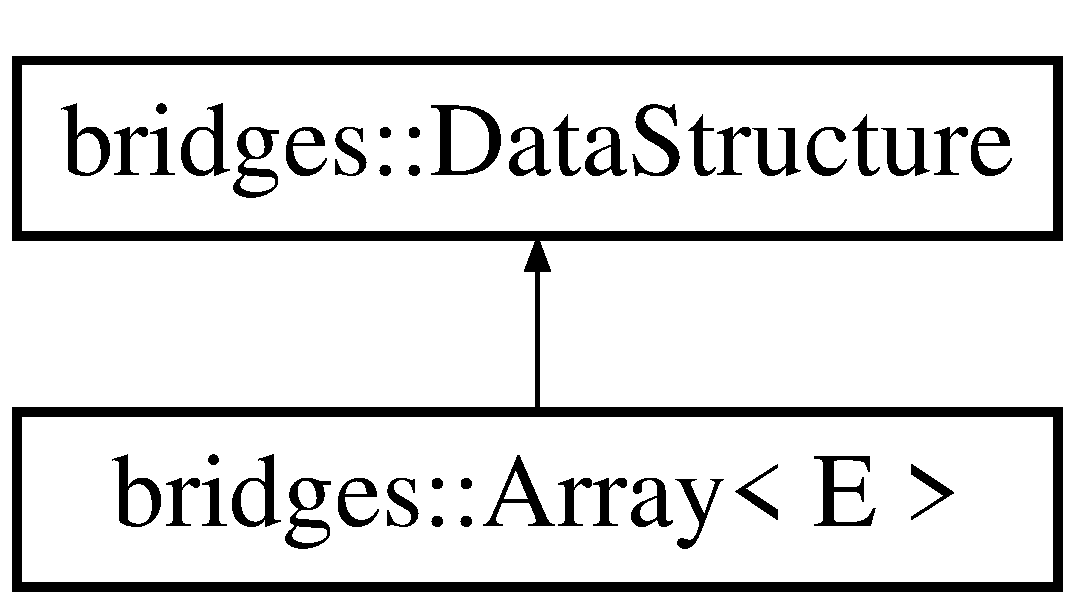
\includegraphics[height=2.000000cm]{classbridges_1_1_array}
\end{center}
\end{figure}
\subsection*{Public Member Functions}
\begin{DoxyCompactItemize}
\item 
\mbox{\hyperlink{classbridges_1_1_array_a958421b86ff55303b5fc7d505109f9fe}{Array}} ()
\item 
\mbox{\hyperlink{classbridges_1_1_array_abfca49c36c2b6c63c88010df50f5f49c}{$\sim$\+Array}} ()
\item 
\mbox{\hyperlink{classbridges_1_1_array_a25ff771f9ba7f365465f309ed2dd3688}{Array}} (int num\+\_\+dims, int $\ast$dims)
\item 
\mbox{\hyperlink{classbridges_1_1_array_a0a475058b73b938f0fd3f577365aca89}{Array}} (int xsize)
\item 
\mbox{\hyperlink{classbridges_1_1_array_a13b26fc4d2ccb19b277b2acc615efce2}{Array}} (int xsize, int ysize)
\item 
\mbox{\hyperlink{classbridges_1_1_array_a3504e71cacffd343edf8b9ea16f75eb4}{Array}} (int xsize, int ysize, int zsize)
\item 
void \mbox{\hyperlink{classbridges_1_1_array_a6b91612bb7b89a563571fd1ea417ef2a}{set\+Num\+Dimensions}} (int nd)
\item 
void \mbox{\hyperlink{classbridges_1_1_array_a4e179915ab7820bbafe9b3433656b182}{set\+Dimensions}} (int $\ast$dim)
\item 
void \mbox{\hyperlink{classbridges_1_1_array_ae195a6f06157e82c68483ff636e30f5e}{get\+Dimensions}} (int $\ast$d)
\item 
\mbox{\hyperlink{classbridges_1_1_element}{Element}}$<$ E $>$ \& \mbox{\hyperlink{classbridges_1_1_array_a8b4c6cc491829d814e0b6b0ce3654417}{get\+Element}} (int x)
\item 
\mbox{\hyperlink{classbridges_1_1_element}{Element}}$<$ E $>$ \& \mbox{\hyperlink{classbridges_1_1_array_acd5e730e0369b1fa699a5907e889f213}{get\+Element}} (int x, int y)
\item 
\mbox{\hyperlink{classbridges_1_1_element}{Element}}$<$ E $>$ \& \mbox{\hyperlink{classbridges_1_1_array_a7006eeac547c391cb7e8eb19c56ae9f6}{get\+Element}} (int x, int y, int z)
\item 
void \mbox{\hyperlink{classbridges_1_1_array_aae8ec0bd850e00593487022bc914afe0}{set\+Element}} (int indx, \mbox{\hyperlink{classbridges_1_1_element}{Element}}$<$ E $>$ el)
\item 
void \mbox{\hyperlink{classbridges_1_1_array_a428cc76d22af71c5ae57dc293780b8ec}{set\+Element}} (int x\+\_\+indx, int y\+\_\+indx, \mbox{\hyperlink{classbridges_1_1_element}{Element}}$<$ E $>$ el)
\item 
void \mbox{\hyperlink{classbridges_1_1_array_a526c3a190b48a338541e5b4667c5eedf}{set\+Element}} (int x\+\_\+indx, int y\+\_\+indx, int z\+\_\+indx, \mbox{\hyperlink{classbridges_1_1_element}{Element}}$<$ E $>$ el)
\item 
virtual const string \mbox{\hyperlink{classbridges_1_1_array_ab93f7379870a7c0bc63490c53d95ba09}{get\+D\+Stype}} () const override
\item 
virtual const pair$<$ string, string $>$ \mbox{\hyperlink{classbridges_1_1_array_ab039fc0b5dd5683bbdf0fe71fce9d317}{get\+Data\+Structure\+Representation}} () const override final
\end{DoxyCompactItemize}
\subsection*{Friends}
\begin{DoxyCompactItemize}
\item 
class \mbox{\hyperlink{classbridges_1_1_array_a8c6ff2a8dd3e27346dd25f588a78828a}{Element$<$ E $>$}}
\end{DoxyCompactItemize}


\subsection{Detailed Description}
\subsubsection*{template$<$typename E$>$\newline
class bridges\+::\+Array$<$ E $>$}

A B\+R\+I\+D\+G\+ES array type. 

This class can be used to create 1D, 2D, and 3D arrays of any type.

Generic Parameters\+: E the application data type

\begin{DoxyAuthor}{Author}
Kalpathi Subramanian 
\end{DoxyAuthor}
\begin{DoxyDate}{Date}
1/14/17 
\end{DoxyDate}


\subsection{Constructor \& Destructor Documentation}
\mbox{\Hypertarget{classbridges_1_1_array_a958421b86ff55303b5fc7d505109f9fe}\label{classbridges_1_1_array_a958421b86ff55303b5fc7d505109f9fe}} 
\index{bridges\+::\+Array@{bridges\+::\+Array}!Array@{Array}}
\index{Array@{Array}!bridges\+::\+Array@{bridges\+::\+Array}}
\subsubsection{\texorpdfstring{Array()}{Array()}\hspace{0.1cm}{\footnotesize\ttfamily [1/5]}}
{\footnotesize\ttfamily template$<$typename E $>$ \\
\mbox{\hyperlink{classbridges_1_1_array}{bridges\+::\+Array}}$<$ E $>$\+::\mbox{\hyperlink{classbridges_1_1_array}{Array}} (\begin{DoxyParamCaption}{ }\end{DoxyParamCaption})\hspace{0.3cm}{\ttfamily [inline]}}

\mbox{\Hypertarget{classbridges_1_1_array_abfca49c36c2b6c63c88010df50f5f49c}\label{classbridges_1_1_array_abfca49c36c2b6c63c88010df50f5f49c}} 
\index{bridges\+::\+Array@{bridges\+::\+Array}!````~Array@{$\sim$\+Array}}
\index{````~Array@{$\sim$\+Array}!bridges\+::\+Array@{bridges\+::\+Array}}
\subsubsection{\texorpdfstring{$\sim$\+Array()}{~Array()}}
{\footnotesize\ttfamily template$<$typename E $>$ \\
\mbox{\hyperlink{classbridges_1_1_array}{bridges\+::\+Array}}$<$ E $>$\+::$\sim$\mbox{\hyperlink{classbridges_1_1_array}{Array}} (\begin{DoxyParamCaption}{ }\end{DoxyParamCaption})\hspace{0.3cm}{\ttfamily [inline]}}

\mbox{\Hypertarget{classbridges_1_1_array_a25ff771f9ba7f365465f309ed2dd3688}\label{classbridges_1_1_array_a25ff771f9ba7f365465f309ed2dd3688}} 
\index{bridges\+::\+Array@{bridges\+::\+Array}!Array@{Array}}
\index{Array@{Array}!bridges\+::\+Array@{bridges\+::\+Array}}
\subsubsection{\texorpdfstring{Array()}{Array()}\hspace{0.1cm}{\footnotesize\ttfamily [2/5]}}
{\footnotesize\ttfamily template$<$typename E $>$ \\
\mbox{\hyperlink{classbridges_1_1_array}{bridges\+::\+Array}}$<$ E $>$\+::\mbox{\hyperlink{classbridges_1_1_array}{Array}} (\begin{DoxyParamCaption}\item[{int}]{num\+\_\+dims,  }\item[{int $\ast$}]{dims }\end{DoxyParamCaption})\hspace{0.3cm}{\ttfamily [inline]}}

\mbox{\Hypertarget{classbridges_1_1_array_a0a475058b73b938f0fd3f577365aca89}\label{classbridges_1_1_array_a0a475058b73b938f0fd3f577365aca89}} 
\index{bridges\+::\+Array@{bridges\+::\+Array}!Array@{Array}}
\index{Array@{Array}!bridges\+::\+Array@{bridges\+::\+Array}}
\subsubsection{\texorpdfstring{Array()}{Array()}\hspace{0.1cm}{\footnotesize\ttfamily [3/5]}}
{\footnotesize\ttfamily template$<$typename E $>$ \\
\mbox{\hyperlink{classbridges_1_1_array}{bridges\+::\+Array}}$<$ E $>$\+::\mbox{\hyperlink{classbridges_1_1_array}{Array}} (\begin{DoxyParamCaption}\item[{int}]{xsize }\end{DoxyParamCaption})\hspace{0.3cm}{\ttfamily [inline]}}

\mbox{\Hypertarget{classbridges_1_1_array_a13b26fc4d2ccb19b277b2acc615efce2}\label{classbridges_1_1_array_a13b26fc4d2ccb19b277b2acc615efce2}} 
\index{bridges\+::\+Array@{bridges\+::\+Array}!Array@{Array}}
\index{Array@{Array}!bridges\+::\+Array@{bridges\+::\+Array}}
\subsubsection{\texorpdfstring{Array()}{Array()}\hspace{0.1cm}{\footnotesize\ttfamily [4/5]}}
{\footnotesize\ttfamily template$<$typename E $>$ \\
\mbox{\hyperlink{classbridges_1_1_array}{bridges\+::\+Array}}$<$ E $>$\+::\mbox{\hyperlink{classbridges_1_1_array}{Array}} (\begin{DoxyParamCaption}\item[{int}]{xsize,  }\item[{int}]{ysize }\end{DoxyParamCaption})\hspace{0.3cm}{\ttfamily [inline]}}

\mbox{\Hypertarget{classbridges_1_1_array_a3504e71cacffd343edf8b9ea16f75eb4}\label{classbridges_1_1_array_a3504e71cacffd343edf8b9ea16f75eb4}} 
\index{bridges\+::\+Array@{bridges\+::\+Array}!Array@{Array}}
\index{Array@{Array}!bridges\+::\+Array@{bridges\+::\+Array}}
\subsubsection{\texorpdfstring{Array()}{Array()}\hspace{0.1cm}{\footnotesize\ttfamily [5/5]}}
{\footnotesize\ttfamily template$<$typename E $>$ \\
\mbox{\hyperlink{classbridges_1_1_array}{bridges\+::\+Array}}$<$ E $>$\+::\mbox{\hyperlink{classbridges_1_1_array}{Array}} (\begin{DoxyParamCaption}\item[{int}]{xsize,  }\item[{int}]{ysize,  }\item[{int}]{zsize }\end{DoxyParamCaption})\hspace{0.3cm}{\ttfamily [inline]}}



\subsection{Member Function Documentation}
\mbox{\Hypertarget{classbridges_1_1_array_ab039fc0b5dd5683bbdf0fe71fce9d317}\label{classbridges_1_1_array_ab039fc0b5dd5683bbdf0fe71fce9d317}} 
\index{bridges\+::\+Array@{bridges\+::\+Array}!get\+Data\+Structure\+Representation@{get\+Data\+Structure\+Representation}}
\index{get\+Data\+Structure\+Representation@{get\+Data\+Structure\+Representation}!bridges\+::\+Array@{bridges\+::\+Array}}
\subsubsection{\texorpdfstring{get\+Data\+Structure\+Representation()}{getDataStructureRepresentation()}}
{\footnotesize\ttfamily template$<$typename E $>$ \\
virtual const pair$<$string, string$>$ \mbox{\hyperlink{classbridges_1_1_array}{bridges\+::\+Array}}$<$ E $>$\+::get\+Data\+Structure\+Representation (\begin{DoxyParamCaption}{ }\end{DoxyParamCaption}) const\hspace{0.3cm}{\ttfamily [inline]}, {\ttfamily [final]}, {\ttfamily [override]}, {\ttfamily [virtual]}}

Gets the J\+S\+ON representation of this \mbox{\hyperlink{classbridges_1_1_data_structure}{Data\+Structure}}\textquotesingle{}s nodes and links


\begin{DoxyParams}{Parameters}
{\em arr\+\_\+size} & The size of the array determined by this \\
\hline
\end{DoxyParams}
\begin{DoxyReturn}{Returns}
A pair holding the nodes and links J\+S\+ON strings respectively 
\end{DoxyReturn}


Implements \mbox{\hyperlink{classbridges_1_1_data_structure}{bridges\+::\+Data\+Structure}}.

\mbox{\Hypertarget{classbridges_1_1_array_ae195a6f06157e82c68483ff636e30f5e}\label{classbridges_1_1_array_ae195a6f06157e82c68483ff636e30f5e}} 
\index{bridges\+::\+Array@{bridges\+::\+Array}!get\+Dimensions@{get\+Dimensions}}
\index{get\+Dimensions@{get\+Dimensions}!bridges\+::\+Array@{bridges\+::\+Array}}
\subsubsection{\texorpdfstring{get\+Dimensions()}{getDimensions()}}
{\footnotesize\ttfamily template$<$typename E $>$ \\
void \mbox{\hyperlink{classbridges_1_1_array}{bridges\+::\+Array}}$<$ E $>$\+::get\+Dimensions (\begin{DoxyParamCaption}\item[{int $\ast$}]{d }\end{DoxyParamCaption})\hspace{0.3cm}{\ttfamily [inline]}}

\mbox{\Hypertarget{classbridges_1_1_array_ab93f7379870a7c0bc63490c53d95ba09}\label{classbridges_1_1_array_ab93f7379870a7c0bc63490c53d95ba09}} 
\index{bridges\+::\+Array@{bridges\+::\+Array}!get\+D\+Stype@{get\+D\+Stype}}
\index{get\+D\+Stype@{get\+D\+Stype}!bridges\+::\+Array@{bridges\+::\+Array}}
\subsubsection{\texorpdfstring{get\+D\+Stype()}{getDStype()}}
{\footnotesize\ttfamily template$<$typename E $>$ \\
virtual const string \mbox{\hyperlink{classbridges_1_1_array}{bridges\+::\+Array}}$<$ E $>$\+::get\+D\+Stype (\begin{DoxyParamCaption}{ }\end{DoxyParamCaption}) const\hspace{0.3cm}{\ttfamily [inline]}, {\ttfamily [override]}, {\ttfamily [virtual]}}

\begin{DoxyReturn}{Returns}
The string representation of this data structure type 
\end{DoxyReturn}


Implements \mbox{\hyperlink{classbridges_1_1_data_structure_a957a63b106e340bc753620c650632bdc}{bridges\+::\+Data\+Structure}}.

\mbox{\Hypertarget{classbridges_1_1_array_a8b4c6cc491829d814e0b6b0ce3654417}\label{classbridges_1_1_array_a8b4c6cc491829d814e0b6b0ce3654417}} 
\index{bridges\+::\+Array@{bridges\+::\+Array}!get\+Element@{get\+Element}}
\index{get\+Element@{get\+Element}!bridges\+::\+Array@{bridges\+::\+Array}}
\subsubsection{\texorpdfstring{get\+Element()}{getElement()}\hspace{0.1cm}{\footnotesize\ttfamily [1/3]}}
{\footnotesize\ttfamily template$<$typename E $>$ \\
\mbox{\hyperlink{classbridges_1_1_element}{Element}}$<$E$>$\& \mbox{\hyperlink{classbridges_1_1_array}{bridges\+::\+Array}}$<$ E $>$\+::get\+Element (\begin{DoxyParamCaption}\item[{int}]{x }\end{DoxyParamCaption})\hspace{0.3cm}{\ttfamily [inline]}}

Get the object at index x -\/ 1D array


\begin{DoxyParams}{Parameters}
{\em x\+\_\+indx} & -\/ index into the array\\
\hline
\end{DoxyParams}
\begin{DoxyReturn}{Returns}
Element$<$\+E$>$ object at \textquotesingle{}indx\textquotesingle{} 
\end{DoxyReturn}
\mbox{\Hypertarget{classbridges_1_1_array_acd5e730e0369b1fa699a5907e889f213}\label{classbridges_1_1_array_acd5e730e0369b1fa699a5907e889f213}} 
\index{bridges\+::\+Array@{bridges\+::\+Array}!get\+Element@{get\+Element}}
\index{get\+Element@{get\+Element}!bridges\+::\+Array@{bridges\+::\+Array}}
\subsubsection{\texorpdfstring{get\+Element()}{getElement()}\hspace{0.1cm}{\footnotesize\ttfamily [2/3]}}
{\footnotesize\ttfamily template$<$typename E $>$ \\
\mbox{\hyperlink{classbridges_1_1_element}{Element}}$<$E$>$\& \mbox{\hyperlink{classbridges_1_1_array}{bridges\+::\+Array}}$<$ E $>$\+::get\+Element (\begin{DoxyParamCaption}\item[{int}]{x,  }\item[{int}]{y }\end{DoxyParamCaption})\hspace{0.3cm}{\ttfamily [inline]}}

Get the object at x, y, z -- for 3D arrays


\begin{DoxyParams}{Parameters}
{\em x} & -\/ column index \\
\hline
{\em y} & -\/ row index\\
\hline
\end{DoxyParams}
\begin{DoxyReturn}{Returns}
Element$<$\+E$>$ object at x, y 
\end{DoxyReturn}
\mbox{\Hypertarget{classbridges_1_1_array_a7006eeac547c391cb7e8eb19c56ae9f6}\label{classbridges_1_1_array_a7006eeac547c391cb7e8eb19c56ae9f6}} 
\index{bridges\+::\+Array@{bridges\+::\+Array}!get\+Element@{get\+Element}}
\index{get\+Element@{get\+Element}!bridges\+::\+Array@{bridges\+::\+Array}}
\subsubsection{\texorpdfstring{get\+Element()}{getElement()}\hspace{0.1cm}{\footnotesize\ttfamily [3/3]}}
{\footnotesize\ttfamily template$<$typename E $>$ \\
\mbox{\hyperlink{classbridges_1_1_element}{Element}}$<$E$>$\& \mbox{\hyperlink{classbridges_1_1_array}{bridges\+::\+Array}}$<$ E $>$\+::get\+Element (\begin{DoxyParamCaption}\item[{int}]{x,  }\item[{int}]{y,  }\item[{int}]{z }\end{DoxyParamCaption})\hspace{0.3cm}{\ttfamily [inline]}}

Get the object at x, y, z -- for 3D arrays


\begin{DoxyParams}{Parameters}
{\em x} & -\/ column index \\
\hline
{\em y} & -\/ row index\\
\hline
\end{DoxyParams}
\begin{DoxyReturn}{Returns}
Element$<$\+E$>$ object at x, y, z 
\end{DoxyReturn}
\mbox{\Hypertarget{classbridges_1_1_array_a4e179915ab7820bbafe9b3433656b182}\label{classbridges_1_1_array_a4e179915ab7820bbafe9b3433656b182}} 
\index{bridges\+::\+Array@{bridges\+::\+Array}!set\+Dimensions@{set\+Dimensions}}
\index{set\+Dimensions@{set\+Dimensions}!bridges\+::\+Array@{bridges\+::\+Array}}
\subsubsection{\texorpdfstring{set\+Dimensions()}{setDimensions()}}
{\footnotesize\ttfamily template$<$typename E $>$ \\
void \mbox{\hyperlink{classbridges_1_1_array}{bridges\+::\+Array}}$<$ E $>$\+::set\+Dimensions (\begin{DoxyParamCaption}\item[{int $\ast$}]{dim }\end{DoxyParamCaption})\hspace{0.3cm}{\ttfamily [inline]}}

\mbox{\Hypertarget{classbridges_1_1_array_aae8ec0bd850e00593487022bc914afe0}\label{classbridges_1_1_array_aae8ec0bd850e00593487022bc914afe0}} 
\index{bridges\+::\+Array@{bridges\+::\+Array}!set\+Element@{set\+Element}}
\index{set\+Element@{set\+Element}!bridges\+::\+Array@{bridges\+::\+Array}}
\subsubsection{\texorpdfstring{set\+Element()}{setElement()}\hspace{0.1cm}{\footnotesize\ttfamily [1/3]}}
{\footnotesize\ttfamily template$<$typename E $>$ \\
void \mbox{\hyperlink{classbridges_1_1_array}{bridges\+::\+Array}}$<$ E $>$\+::set\+Element (\begin{DoxyParamCaption}\item[{int}]{indx,  }\item[{\mbox{\hyperlink{classbridges_1_1_element}{Element}}$<$ E $>$}]{el }\end{DoxyParamCaption})\hspace{0.3cm}{\ttfamily [inline]}}

Set the object at index x -\/ 1D array


\begin{DoxyParams}{Parameters}
{\em x} & -\/ index into the array  -\/ \mbox{\hyperlink{classbridges_1_1_element}{Element}} object\\
\hline
\end{DoxyParams}
\begin{DoxyReturn}{Returns}
none 
\end{DoxyReturn}
\mbox{\Hypertarget{classbridges_1_1_array_a428cc76d22af71c5ae57dc293780b8ec}\label{classbridges_1_1_array_a428cc76d22af71c5ae57dc293780b8ec}} 
\index{bridges\+::\+Array@{bridges\+::\+Array}!set\+Element@{set\+Element}}
\index{set\+Element@{set\+Element}!bridges\+::\+Array@{bridges\+::\+Array}}
\subsubsection{\texorpdfstring{set\+Element()}{setElement()}\hspace{0.1cm}{\footnotesize\ttfamily [2/3]}}
{\footnotesize\ttfamily template$<$typename E $>$ \\
void \mbox{\hyperlink{classbridges_1_1_array}{bridges\+::\+Array}}$<$ E $>$\+::set\+Element (\begin{DoxyParamCaption}\item[{int}]{x\+\_\+indx,  }\item[{int}]{y\+\_\+indx,  }\item[{\mbox{\hyperlink{classbridges_1_1_element}{Element}}$<$ E $>$}]{el }\end{DoxyParamCaption})\hspace{0.3cm}{\ttfamily [inline]}}

Set the object at index x, y -\/ 2D array


\begin{DoxyParams}{Parameters}
{\em x} & -\/ col index into the array \\
\hline
{\em y} & -\/ row index into the array  -\/ \mbox{\hyperlink{classbridges_1_1_element}{Element}} object\\
\hline
\end{DoxyParams}
\begin{DoxyReturn}{Returns}
none 
\end{DoxyReturn}
\mbox{\Hypertarget{classbridges_1_1_array_a526c3a190b48a338541e5b4667c5eedf}\label{classbridges_1_1_array_a526c3a190b48a338541e5b4667c5eedf}} 
\index{bridges\+::\+Array@{bridges\+::\+Array}!set\+Element@{set\+Element}}
\index{set\+Element@{set\+Element}!bridges\+::\+Array@{bridges\+::\+Array}}
\subsubsection{\texorpdfstring{set\+Element()}{setElement()}\hspace{0.1cm}{\footnotesize\ttfamily [3/3]}}
{\footnotesize\ttfamily template$<$typename E $>$ \\
void \mbox{\hyperlink{classbridges_1_1_array}{bridges\+::\+Array}}$<$ E $>$\+::set\+Element (\begin{DoxyParamCaption}\item[{int}]{x\+\_\+indx,  }\item[{int}]{y\+\_\+indx,  }\item[{int}]{z\+\_\+indx,  }\item[{\mbox{\hyperlink{classbridges_1_1_element}{Element}}$<$ E $>$}]{el }\end{DoxyParamCaption})\hspace{0.3cm}{\ttfamily [inline]}}

Set the object at index x, y, z -\/ 3D array


\begin{DoxyParams}{Parameters}
{\em x} & -\/ col index into the array \\
\hline
{\em y} & -\/ row index into the array \\
\hline
{\em z} & -\/ slice index into the array  -\/ \mbox{\hyperlink{classbridges_1_1_element}{Element}} object\\
\hline
\end{DoxyParams}
\begin{DoxyReturn}{Returns}
none 
\end{DoxyReturn}
\mbox{\Hypertarget{classbridges_1_1_array_a6b91612bb7b89a563571fd1ea417ef2a}\label{classbridges_1_1_array_a6b91612bb7b89a563571fd1ea417ef2a}} 
\index{bridges\+::\+Array@{bridges\+::\+Array}!set\+Num\+Dimensions@{set\+Num\+Dimensions}}
\index{set\+Num\+Dimensions@{set\+Num\+Dimensions}!bridges\+::\+Array@{bridges\+::\+Array}}
\subsubsection{\texorpdfstring{set\+Num\+Dimensions()}{setNumDimensions()}}
{\footnotesize\ttfamily template$<$typename E $>$ \\
void \mbox{\hyperlink{classbridges_1_1_array}{bridges\+::\+Array}}$<$ E $>$\+::set\+Num\+Dimensions (\begin{DoxyParamCaption}\item[{int}]{nd }\end{DoxyParamCaption})\hspace{0.3cm}{\ttfamily [inline]}}



\subsection{Friends And Related Function Documentation}
\mbox{\Hypertarget{classbridges_1_1_array_a8c6ff2a8dd3e27346dd25f588a78828a}\label{classbridges_1_1_array_a8c6ff2a8dd3e27346dd25f588a78828a}} 
\index{bridges\+::\+Array@{bridges\+::\+Array}!Element$<$ E $>$@{Element$<$ E $>$}}
\index{Element$<$ E $>$@{Element$<$ E $>$}!bridges\+::\+Array@{bridges\+::\+Array}}
\subsubsection{\texorpdfstring{Element$<$ E $>$}{Element< E >}}
{\footnotesize\ttfamily template$<$typename E $>$ \\
friend class \mbox{\hyperlink{classbridges_1_1_element}{Element}}$<$ E $>$\hspace{0.3cm}{\ttfamily [friend]}}



The documentation for this class was generated from the following file\+:\begin{DoxyCompactItemize}
\item 
/\+Users/kalpathi/gr/bridges/client/cxx/bridges17/src/\mbox{\hyperlink{_array_8h}{Array.\+h}}\end{DoxyCompactItemize}

\hypertarget{classbridges_1_1_a_v_l_tree_element}{}\section{bridges\+::A\+V\+L\+Tree\+Element$<$ K, E $>$ Class Template Reference}
\label{classbridges_1_1_a_v_l_tree_element}\index{bridges::AVLTreeElement$<$ K, E $>$@{bridges::AVLTreeElement$<$ K, E $>$}}


This class can be used to create avl tree elements, derived from \mbox{\hyperlink{classbridges_1_1_b_s_t_element}{B\+S\+T\+Element}}.  




{\ttfamily \#include $<$A\+V\+L\+Tree\+Element.\+h$>$}

Inheritance diagram for bridges\+::A\+V\+L\+Tree\+Element$<$ K, E $>$\+:\begin{figure}[H]
\begin{center}
\leavevmode
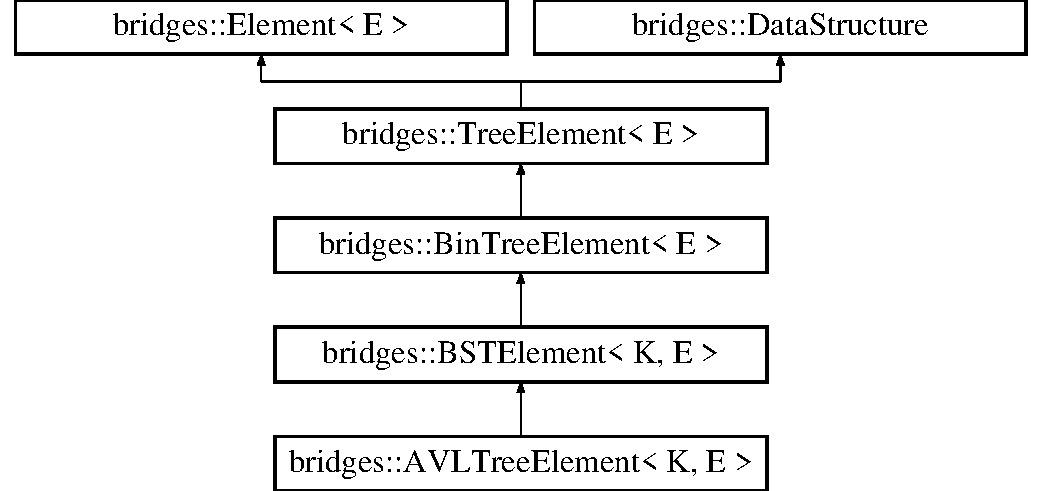
\includegraphics[height=5.000000cm]{classbridges_1_1_a_v_l_tree_element}
\end{center}
\end{figure}
\subsection*{Public Member Functions}
\begin{DoxyCompactItemize}
\item 
\mbox{\hyperlink{classbridges_1_1_a_v_l_tree_element_a24d1dfb65f00f2fef96a57a3f869a263}{A\+V\+L\+Tree\+Element}} (const \mbox{\hyperlink{namespacebridges_acfb0a4f7877d8f63de3e6862004c50edaa5f3c6a11b03839d46af9fb43c97c188}{K}} \&\mbox{\hyperlink{namespacebridges_acfb0a4f7877d8f63de3e6862004c50eda8ce4b16b22b58894aa86c421e8759df3}{k}}, const \mbox{\hyperlink{namespacebridges_acfb0a4f7877d8f63de3e6862004c50eda3a3ea00cfc35332cedf6e5e9a32e94da}{E}} \&val=\mbox{\hyperlink{namespacebridges_acfb0a4f7877d8f63de3e6862004c50eda3a3ea00cfc35332cedf6e5e9a32e94da}{E}}(), const string \&lab=string())
\item 
virtual const string \mbox{\hyperlink{classbridges_1_1_a_v_l_tree_element_a24c005f8e07a7a2682225cead3b7e364}{get\+D\+Stype}} () const override
\item 
int \mbox{\hyperlink{classbridges_1_1_a_v_l_tree_element_ace72b436fa14db4f7844cc6e30b87aa7}{get\+Height}} () const
\item 
void \mbox{\hyperlink{classbridges_1_1_a_v_l_tree_element_acbf2a222b954e5d9221b109634822f96}{set\+Height}} (const int \&\mbox{\hyperlink{namespacebridges_acfb0a4f7877d8f63de3e6862004c50eda2510c39011c5be704182423e3a695e91}{h}})
\item 
int \mbox{\hyperlink{classbridges_1_1_a_v_l_tree_element_aa37dc257fbc32ad8bfdd885bf98d3a8d}{get\+Balance\+Factor}} () const
\item 
void \mbox{\hyperlink{classbridges_1_1_a_v_l_tree_element_a076ec482874d248764348e62dd4652d2}{set\+Balance\+Factor}} (const int \&bf)
\item 
virtual \mbox{\hyperlink{classbridges_1_1_a_v_l_tree_element}{A\+V\+L\+Tree\+Element}} $\ast$ \mbox{\hyperlink{classbridges_1_1_a_v_l_tree_element_a7b5d05660da127f5f6164120d9846d90}{get\+Left}} () override
\item 
virtual const \mbox{\hyperlink{classbridges_1_1_a_v_l_tree_element}{A\+V\+L\+Tree\+Element}} $\ast$ \mbox{\hyperlink{classbridges_1_1_a_v_l_tree_element_a61e075db5414b7bd6f52d657401acda3}{get\+Left}} () const override
\item 
void \mbox{\hyperlink{classbridges_1_1_a_v_l_tree_element_a19980980e712d10a1158272ecc44ef10}{set\+Left}} (\mbox{\hyperlink{classbridges_1_1_a_v_l_tree_element}{A\+V\+L\+Tree\+Element}} $\ast$\mbox{\hyperlink{namespacebridges_acfb0a4f7877d8f63de3e6862004c50eda2db95e8e1a9267b7a1188556b2013b33}{l}})
\item 
virtual \mbox{\hyperlink{classbridges_1_1_a_v_l_tree_element}{A\+V\+L\+Tree\+Element}} $\ast$ \mbox{\hyperlink{classbridges_1_1_a_v_l_tree_element_a909b46ebf3e8c6a3434762a1f01499e2}{get\+Right}} () override
\item 
virtual const \mbox{\hyperlink{classbridges_1_1_a_v_l_tree_element}{A\+V\+L\+Tree\+Element}} $\ast$ \mbox{\hyperlink{classbridges_1_1_a_v_l_tree_element_a2f6fd127f3a04fcc5be60299b7d98f12}{get\+Right}} () const override
\item 
void \mbox{\hyperlink{classbridges_1_1_a_v_l_tree_element_a2e048abe8e79232effa92dfdbeac4a54}{set\+Right}} (\mbox{\hyperlink{classbridges_1_1_a_v_l_tree_element}{A\+V\+L\+Tree\+Element}} $\ast$\mbox{\hyperlink{namespacebridges_acfb0a4f7877d8f63de3e6862004c50eda4b43b0aee35624cd95b910189b3dc231}{r}})
\end{DoxyCompactItemize}
\subsection*{Additional Inherited Members}


\subsection{Detailed Description}
\subsubsection*{template$<$typename K, typename E$>$\newline
class bridges\+::\+A\+V\+L\+Tree\+Element$<$ K, E $>$}

This class can be used to create avl tree elements, derived from \mbox{\hyperlink{classbridges_1_1_b_s_t_element}{B\+S\+T\+Element}}. 

This class extends the \mbox{\hyperlink{classbridges_1_1_b_s_t_element}{B\+S\+T\+Element}} class by adding height and balance factor attributes to allow for easier use in a avl tree implementation.

Generic Parameters\+: K that is the search key type, E the application data type

\begin{DoxyAuthor}{Author}
Kalpathi Subramanian 
\end{DoxyAuthor}
\begin{DoxyDate}{Date}
6/18/15, 7/15/16 
\end{DoxyDate}


\subsection{Constructor \& Destructor Documentation}
\mbox{\Hypertarget{classbridges_1_1_a_v_l_tree_element_a24d1dfb65f00f2fef96a57a3f869a263}\label{classbridges_1_1_a_v_l_tree_element_a24d1dfb65f00f2fef96a57a3f869a263}} 
\index{bridges::AVLTreeElement$<$ K, E $>$@{bridges::AVLTreeElement$<$ K, E $>$}!AVLTreeElement@{AVLTreeElement}}
\index{AVLTreeElement@{AVLTreeElement}!bridges::AVLTreeElement$<$ K, E $>$@{bridges::AVLTreeElement$<$ K, E $>$}}
\subsubsection{\texorpdfstring{AVLTreeElement()}{AVLTreeElement()}}
{\footnotesize\ttfamily template$<$typename K , typename E $>$ \\
\mbox{\hyperlink{classbridges_1_1_a_v_l_tree_element}{bridges\+::\+A\+V\+L\+Tree\+Element}}$<$ \mbox{\hyperlink{namespacebridges_acfb0a4f7877d8f63de3e6862004c50edaa5f3c6a11b03839d46af9fb43c97c188}{K}}, \mbox{\hyperlink{namespacebridges_acfb0a4f7877d8f63de3e6862004c50eda3a3ea00cfc35332cedf6e5e9a32e94da}{E}} $>$\+::\mbox{\hyperlink{classbridges_1_1_a_v_l_tree_element}{A\+V\+L\+Tree\+Element}} (\begin{DoxyParamCaption}\item[{const \mbox{\hyperlink{namespacebridges_acfb0a4f7877d8f63de3e6862004c50edaa5f3c6a11b03839d46af9fb43c97c188}{K}} \&}]{k,  }\item[{const \mbox{\hyperlink{namespacebridges_acfb0a4f7877d8f63de3e6862004c50eda3a3ea00cfc35332cedf6e5e9a32e94da}{E}} \&}]{val = {\ttfamily \mbox{\hyperlink{namespacebridges_acfb0a4f7877d8f63de3e6862004c50eda3a3ea00cfc35332cedf6e5e9a32e94da}{E}}()},  }\item[{const string \&}]{lab = {\ttfamily string()} }\end{DoxyParamCaption})\hspace{0.3cm}{\ttfamily [inline]}}

Constructs a \mbox{\hyperlink{classbridges_1_1_a_v_l_tree_element}{A\+V\+L\+Tree\+Element}} with the provided value, label, key, setting the left and right A\+V\+L\+Tree\+Elements to N\+U\+LL. The defaults will be used if not provided.


\begin{DoxyParams}{Parameters}
{\em val} & The data to hold \\
\hline
{\em lab} & The label to show \\
\hline
{\em k} & The key for ordering \\
\hline
\end{DoxyParams}


\subsection{Member Function Documentation}
\mbox{\Hypertarget{classbridges_1_1_a_v_l_tree_element_aa37dc257fbc32ad8bfdd885bf98d3a8d}\label{classbridges_1_1_a_v_l_tree_element_aa37dc257fbc32ad8bfdd885bf98d3a8d}} 
\index{bridges::AVLTreeElement$<$ K, E $>$@{bridges::AVLTreeElement$<$ K, E $>$}!getBalanceFactor@{getBalanceFactor}}
\index{getBalanceFactor@{getBalanceFactor}!bridges::AVLTreeElement$<$ K, E $>$@{bridges::AVLTreeElement$<$ K, E $>$}}
\subsubsection{\texorpdfstring{getBalanceFactor()}{getBalanceFactor()}}
{\footnotesize\ttfamily template$<$typename K , typename E $>$ \\
int \mbox{\hyperlink{classbridges_1_1_a_v_l_tree_element}{bridges\+::\+A\+V\+L\+Tree\+Element}}$<$ \mbox{\hyperlink{namespacebridges_acfb0a4f7877d8f63de3e6862004c50edaa5f3c6a11b03839d46af9fb43c97c188}{K}}, \mbox{\hyperlink{namespacebridges_acfb0a4f7877d8f63de3e6862004c50eda3a3ea00cfc35332cedf6e5e9a32e94da}{E}} $>$\+::get\+Balance\+Factor (\begin{DoxyParamCaption}{ }\end{DoxyParamCaption}) const\hspace{0.3cm}{\ttfamily [inline]}}

\begin{DoxyReturn}{Returns}
The balance factor of this \mbox{\hyperlink{classbridges_1_1_a_v_l_tree_element}{A\+V\+L\+Tree\+Element}} 
\end{DoxyReturn}
\mbox{\Hypertarget{classbridges_1_1_a_v_l_tree_element_a24c005f8e07a7a2682225cead3b7e364}\label{classbridges_1_1_a_v_l_tree_element_a24c005f8e07a7a2682225cead3b7e364}} 
\index{bridges::AVLTreeElement$<$ K, E $>$@{bridges::AVLTreeElement$<$ K, E $>$}!getDStype@{getDStype}}
\index{getDStype@{getDStype}!bridges::AVLTreeElement$<$ K, E $>$@{bridges::AVLTreeElement$<$ K, E $>$}}
\subsubsection{\texorpdfstring{getDStype()}{getDStype()}}
{\footnotesize\ttfamily template$<$typename K , typename E $>$ \\
virtual const string \mbox{\hyperlink{classbridges_1_1_a_v_l_tree_element}{bridges\+::\+A\+V\+L\+Tree\+Element}}$<$ \mbox{\hyperlink{namespacebridges_acfb0a4f7877d8f63de3e6862004c50edaa5f3c6a11b03839d46af9fb43c97c188}{K}}, \mbox{\hyperlink{namespacebridges_acfb0a4f7877d8f63de3e6862004c50eda3a3ea00cfc35332cedf6e5e9a32e94da}{E}} $>$\+::get\+D\+Stype (\begin{DoxyParamCaption}{ }\end{DoxyParamCaption}) const\hspace{0.3cm}{\ttfamily [inline]}, {\ttfamily [override]}, {\ttfamily [virtual]}}

\begin{DoxyReturn}{Returns}
the data structure type 
\end{DoxyReturn}


Reimplemented from \mbox{\hyperlink{classbridges_1_1_b_s_t_element_af3843873c508c24f90b6e73a6f490bf8}{bridges\+::\+B\+S\+T\+Element$<$ K, E $>$}}.

\mbox{\Hypertarget{classbridges_1_1_a_v_l_tree_element_ace72b436fa14db4f7844cc6e30b87aa7}\label{classbridges_1_1_a_v_l_tree_element_ace72b436fa14db4f7844cc6e30b87aa7}} 
\index{bridges::AVLTreeElement$<$ K, E $>$@{bridges::AVLTreeElement$<$ K, E $>$}!getHeight@{getHeight}}
\index{getHeight@{getHeight}!bridges::AVLTreeElement$<$ K, E $>$@{bridges::AVLTreeElement$<$ K, E $>$}}
\subsubsection{\texorpdfstring{getHeight()}{getHeight()}}
{\footnotesize\ttfamily template$<$typename K , typename E $>$ \\
int \mbox{\hyperlink{classbridges_1_1_a_v_l_tree_element}{bridges\+::\+A\+V\+L\+Tree\+Element}}$<$ \mbox{\hyperlink{namespacebridges_acfb0a4f7877d8f63de3e6862004c50edaa5f3c6a11b03839d46af9fb43c97c188}{K}}, \mbox{\hyperlink{namespacebridges_acfb0a4f7877d8f63de3e6862004c50eda3a3ea00cfc35332cedf6e5e9a32e94da}{E}} $>$\+::get\+Height (\begin{DoxyParamCaption}{ }\end{DoxyParamCaption}) const\hspace{0.3cm}{\ttfamily [inline]}}

\begin{DoxyReturn}{Returns}
The height of this \mbox{\hyperlink{classbridges_1_1_a_v_l_tree_element}{A\+V\+L\+Tree\+Element}} 
\end{DoxyReturn}
\mbox{\Hypertarget{classbridges_1_1_a_v_l_tree_element_a7b5d05660da127f5f6164120d9846d90}\label{classbridges_1_1_a_v_l_tree_element_a7b5d05660da127f5f6164120d9846d90}} 
\index{bridges::AVLTreeElement$<$ K, E $>$@{bridges::AVLTreeElement$<$ K, E $>$}!getLeft@{getLeft}}
\index{getLeft@{getLeft}!bridges::AVLTreeElement$<$ K, E $>$@{bridges::AVLTreeElement$<$ K, E $>$}}
\subsubsection{\texorpdfstring{getLeft()}{getLeft()}\hspace{0.1cm}{\footnotesize\ttfamily [1/2]}}
{\footnotesize\ttfamily template$<$typename K , typename E $>$ \\
virtual \mbox{\hyperlink{classbridges_1_1_a_v_l_tree_element}{A\+V\+L\+Tree\+Element}}$\ast$ \mbox{\hyperlink{classbridges_1_1_a_v_l_tree_element}{bridges\+::\+A\+V\+L\+Tree\+Element}}$<$ \mbox{\hyperlink{namespacebridges_acfb0a4f7877d8f63de3e6862004c50edaa5f3c6a11b03839d46af9fb43c97c188}{K}}, \mbox{\hyperlink{namespacebridges_acfb0a4f7877d8f63de3e6862004c50eda3a3ea00cfc35332cedf6e5e9a32e94da}{E}} $>$\+::get\+Left (\begin{DoxyParamCaption}{ }\end{DoxyParamCaption})\hspace{0.3cm}{\ttfamily [inline]}, {\ttfamily [override]}, {\ttfamily [virtual]}}

\begin{DoxyReturn}{Returns}
The left child 
\end{DoxyReturn}


Reimplemented from \mbox{\hyperlink{classbridges_1_1_b_s_t_element_a4d8987373c75b51fca94e3c0b78b87a6}{bridges\+::\+B\+S\+T\+Element$<$ K, E $>$}}.

\mbox{\Hypertarget{classbridges_1_1_a_v_l_tree_element_a61e075db5414b7bd6f52d657401acda3}\label{classbridges_1_1_a_v_l_tree_element_a61e075db5414b7bd6f52d657401acda3}} 
\index{bridges::AVLTreeElement$<$ K, E $>$@{bridges::AVLTreeElement$<$ K, E $>$}!getLeft@{getLeft}}
\index{getLeft@{getLeft}!bridges::AVLTreeElement$<$ K, E $>$@{bridges::AVLTreeElement$<$ K, E $>$}}
\subsubsection{\texorpdfstring{getLeft()}{getLeft()}\hspace{0.1cm}{\footnotesize\ttfamily [2/2]}}
{\footnotesize\ttfamily template$<$typename K , typename E $>$ \\
virtual const \mbox{\hyperlink{classbridges_1_1_a_v_l_tree_element}{A\+V\+L\+Tree\+Element}}$\ast$ \mbox{\hyperlink{classbridges_1_1_a_v_l_tree_element}{bridges\+::\+A\+V\+L\+Tree\+Element}}$<$ \mbox{\hyperlink{namespacebridges_acfb0a4f7877d8f63de3e6862004c50edaa5f3c6a11b03839d46af9fb43c97c188}{K}}, \mbox{\hyperlink{namespacebridges_acfb0a4f7877d8f63de3e6862004c50eda3a3ea00cfc35332cedf6e5e9a32e94da}{E}} $>$\+::get\+Left (\begin{DoxyParamCaption}{ }\end{DoxyParamCaption}) const\hspace{0.3cm}{\ttfamily [inline]}, {\ttfamily [override]}, {\ttfamily [virtual]}}

Constant version

\begin{DoxyReturn}{Returns}
The left child 
\end{DoxyReturn}


Reimplemented from \mbox{\hyperlink{classbridges_1_1_b_s_t_element_a2abcfb991f6cc377da2bd9217319fc9c}{bridges\+::\+B\+S\+T\+Element$<$ K, E $>$}}.

\mbox{\Hypertarget{classbridges_1_1_a_v_l_tree_element_a909b46ebf3e8c6a3434762a1f01499e2}\label{classbridges_1_1_a_v_l_tree_element_a909b46ebf3e8c6a3434762a1f01499e2}} 
\index{bridges::AVLTreeElement$<$ K, E $>$@{bridges::AVLTreeElement$<$ K, E $>$}!getRight@{getRight}}
\index{getRight@{getRight}!bridges::AVLTreeElement$<$ K, E $>$@{bridges::AVLTreeElement$<$ K, E $>$}}
\subsubsection{\texorpdfstring{getRight()}{getRight()}\hspace{0.1cm}{\footnotesize\ttfamily [1/2]}}
{\footnotesize\ttfamily template$<$typename K , typename E $>$ \\
virtual \mbox{\hyperlink{classbridges_1_1_a_v_l_tree_element}{A\+V\+L\+Tree\+Element}}$\ast$ \mbox{\hyperlink{classbridges_1_1_a_v_l_tree_element}{bridges\+::\+A\+V\+L\+Tree\+Element}}$<$ \mbox{\hyperlink{namespacebridges_acfb0a4f7877d8f63de3e6862004c50edaa5f3c6a11b03839d46af9fb43c97c188}{K}}, \mbox{\hyperlink{namespacebridges_acfb0a4f7877d8f63de3e6862004c50eda3a3ea00cfc35332cedf6e5e9a32e94da}{E}} $>$\+::get\+Right (\begin{DoxyParamCaption}{ }\end{DoxyParamCaption})\hspace{0.3cm}{\ttfamily [inline]}, {\ttfamily [override]}, {\ttfamily [virtual]}}

\begin{DoxyReturn}{Returns}
The right child 
\end{DoxyReturn}


Reimplemented from \mbox{\hyperlink{classbridges_1_1_b_s_t_element_a35e93bce32de933522dccde5f2b5ffd9}{bridges\+::\+B\+S\+T\+Element$<$ K, E $>$}}.

\mbox{\Hypertarget{classbridges_1_1_a_v_l_tree_element_a2f6fd127f3a04fcc5be60299b7d98f12}\label{classbridges_1_1_a_v_l_tree_element_a2f6fd127f3a04fcc5be60299b7d98f12}} 
\index{bridges::AVLTreeElement$<$ K, E $>$@{bridges::AVLTreeElement$<$ K, E $>$}!getRight@{getRight}}
\index{getRight@{getRight}!bridges::AVLTreeElement$<$ K, E $>$@{bridges::AVLTreeElement$<$ K, E $>$}}
\subsubsection{\texorpdfstring{getRight()}{getRight()}\hspace{0.1cm}{\footnotesize\ttfamily [2/2]}}
{\footnotesize\ttfamily template$<$typename K , typename E $>$ \\
virtual const \mbox{\hyperlink{classbridges_1_1_a_v_l_tree_element}{A\+V\+L\+Tree\+Element}}$\ast$ \mbox{\hyperlink{classbridges_1_1_a_v_l_tree_element}{bridges\+::\+A\+V\+L\+Tree\+Element}}$<$ \mbox{\hyperlink{namespacebridges_acfb0a4f7877d8f63de3e6862004c50edaa5f3c6a11b03839d46af9fb43c97c188}{K}}, \mbox{\hyperlink{namespacebridges_acfb0a4f7877d8f63de3e6862004c50eda3a3ea00cfc35332cedf6e5e9a32e94da}{E}} $>$\+::get\+Right (\begin{DoxyParamCaption}{ }\end{DoxyParamCaption}) const\hspace{0.3cm}{\ttfamily [inline]}, {\ttfamily [override]}, {\ttfamily [virtual]}}

Constant version

\begin{DoxyReturn}{Returns}
The right child 
\end{DoxyReturn}


Reimplemented from \mbox{\hyperlink{classbridges_1_1_b_s_t_element_ae4e7b750eada97074a42e7f54b320a29}{bridges\+::\+B\+S\+T\+Element$<$ K, E $>$}}.

\mbox{\Hypertarget{classbridges_1_1_a_v_l_tree_element_a076ec482874d248764348e62dd4652d2}\label{classbridges_1_1_a_v_l_tree_element_a076ec482874d248764348e62dd4652d2}} 
\index{bridges::AVLTreeElement$<$ K, E $>$@{bridges::AVLTreeElement$<$ K, E $>$}!setBalanceFactor@{setBalanceFactor}}
\index{setBalanceFactor@{setBalanceFactor}!bridges::AVLTreeElement$<$ K, E $>$@{bridges::AVLTreeElement$<$ K, E $>$}}
\subsubsection{\texorpdfstring{setBalanceFactor()}{setBalanceFactor()}}
{\footnotesize\ttfamily template$<$typename K , typename E $>$ \\
void \mbox{\hyperlink{classbridges_1_1_a_v_l_tree_element}{bridges\+::\+A\+V\+L\+Tree\+Element}}$<$ \mbox{\hyperlink{namespacebridges_acfb0a4f7877d8f63de3e6862004c50edaa5f3c6a11b03839d46af9fb43c97c188}{K}}, \mbox{\hyperlink{namespacebridges_acfb0a4f7877d8f63de3e6862004c50eda3a3ea00cfc35332cedf6e5e9a32e94da}{E}} $>$\+::set\+Balance\+Factor (\begin{DoxyParamCaption}\item[{const int \&}]{bf }\end{DoxyParamCaption})\hspace{0.3cm}{\ttfamily [inline]}}

Set the balance factor to \char`\"{}bf\char`\"{}
\begin{DoxyParams}{Parameters}
{\em bf} & The balance factor of this \mbox{\hyperlink{classbridges_1_1_a_v_l_tree_element}{A\+V\+L\+Tree\+Element}}\\
\hline
{\em bf} & the balance factor to set at this node \\
\hline
\end{DoxyParams}
\mbox{\Hypertarget{classbridges_1_1_a_v_l_tree_element_acbf2a222b954e5d9221b109634822f96}\label{classbridges_1_1_a_v_l_tree_element_acbf2a222b954e5d9221b109634822f96}} 
\index{bridges::AVLTreeElement$<$ K, E $>$@{bridges::AVLTreeElement$<$ K, E $>$}!setHeight@{setHeight}}
\index{setHeight@{setHeight}!bridges::AVLTreeElement$<$ K, E $>$@{bridges::AVLTreeElement$<$ K, E $>$}}
\subsubsection{\texorpdfstring{setHeight()}{setHeight()}}
{\footnotesize\ttfamily template$<$typename K , typename E $>$ \\
void \mbox{\hyperlink{classbridges_1_1_a_v_l_tree_element}{bridges\+::\+A\+V\+L\+Tree\+Element}}$<$ \mbox{\hyperlink{namespacebridges_acfb0a4f7877d8f63de3e6862004c50edaa5f3c6a11b03839d46af9fb43c97c188}{K}}, \mbox{\hyperlink{namespacebridges_acfb0a4f7877d8f63de3e6862004c50eda3a3ea00cfc35332cedf6e5e9a32e94da}{E}} $>$\+::set\+Height (\begin{DoxyParamCaption}\item[{const int \&}]{h }\end{DoxyParamCaption})\hspace{0.3cm}{\ttfamily [inline]}}

Set the height to \char`\"{}h\char`\"{}
\begin{DoxyParams}{Parameters}
{\em h} & The height of this \mbox{\hyperlink{classbridges_1_1_a_v_l_tree_element}{A\+V\+L\+Tree\+Element}}\\
\hline
{\em h} & the height of the tree at this node \\
\hline
\end{DoxyParams}
\mbox{\Hypertarget{classbridges_1_1_a_v_l_tree_element_a19980980e712d10a1158272ecc44ef10}\label{classbridges_1_1_a_v_l_tree_element_a19980980e712d10a1158272ecc44ef10}} 
\index{bridges::AVLTreeElement$<$ K, E $>$@{bridges::AVLTreeElement$<$ K, E $>$}!setLeft@{setLeft}}
\index{setLeft@{setLeft}!bridges::AVLTreeElement$<$ K, E $>$@{bridges::AVLTreeElement$<$ K, E $>$}}
\subsubsection{\texorpdfstring{setLeft()}{setLeft()}}
{\footnotesize\ttfamily template$<$typename K , typename E $>$ \\
void \mbox{\hyperlink{classbridges_1_1_a_v_l_tree_element}{bridges\+::\+A\+V\+L\+Tree\+Element}}$<$ \mbox{\hyperlink{namespacebridges_acfb0a4f7877d8f63de3e6862004c50edaa5f3c6a11b03839d46af9fb43c97c188}{K}}, \mbox{\hyperlink{namespacebridges_acfb0a4f7877d8f63de3e6862004c50eda3a3ea00cfc35332cedf6e5e9a32e94da}{E}} $>$\+::set\+Left (\begin{DoxyParamCaption}\item[{\mbox{\hyperlink{classbridges_1_1_a_v_l_tree_element}{A\+V\+L\+Tree\+Element}}$<$ \mbox{\hyperlink{namespacebridges_acfb0a4f7877d8f63de3e6862004c50edaa5f3c6a11b03839d46af9fb43c97c188}{K}}, \mbox{\hyperlink{namespacebridges_acfb0a4f7877d8f63de3e6862004c50eda3a3ea00cfc35332cedf6e5e9a32e94da}{E}} $>$ $\ast$}]{l }\end{DoxyParamCaption})\hspace{0.3cm}{\ttfamily [inline]}}

Sets left to \char`\"{}l\char`\"{}


\begin{DoxyParams}{Parameters}
{\em l} & The left tree element \\
\hline
\end{DoxyParams}
\mbox{\Hypertarget{classbridges_1_1_a_v_l_tree_element_a2e048abe8e79232effa92dfdbeac4a54}\label{classbridges_1_1_a_v_l_tree_element_a2e048abe8e79232effa92dfdbeac4a54}} 
\index{bridges::AVLTreeElement$<$ K, E $>$@{bridges::AVLTreeElement$<$ K, E $>$}!setRight@{setRight}}
\index{setRight@{setRight}!bridges::AVLTreeElement$<$ K, E $>$@{bridges::AVLTreeElement$<$ K, E $>$}}
\subsubsection{\texorpdfstring{setRight()}{setRight()}}
{\footnotesize\ttfamily template$<$typename K , typename E $>$ \\
void \mbox{\hyperlink{classbridges_1_1_a_v_l_tree_element}{bridges\+::\+A\+V\+L\+Tree\+Element}}$<$ \mbox{\hyperlink{namespacebridges_acfb0a4f7877d8f63de3e6862004c50edaa5f3c6a11b03839d46af9fb43c97c188}{K}}, \mbox{\hyperlink{namespacebridges_acfb0a4f7877d8f63de3e6862004c50eda3a3ea00cfc35332cedf6e5e9a32e94da}{E}} $>$\+::set\+Right (\begin{DoxyParamCaption}\item[{\mbox{\hyperlink{classbridges_1_1_a_v_l_tree_element}{A\+V\+L\+Tree\+Element}}$<$ \mbox{\hyperlink{namespacebridges_acfb0a4f7877d8f63de3e6862004c50edaa5f3c6a11b03839d46af9fb43c97c188}{K}}, \mbox{\hyperlink{namespacebridges_acfb0a4f7877d8f63de3e6862004c50eda3a3ea00cfc35332cedf6e5e9a32e94da}{E}} $>$ $\ast$}]{r }\end{DoxyParamCaption})\hspace{0.3cm}{\ttfamily [inline]}}

Sets right to \char`\"{}r\char`\"{}


\begin{DoxyParams}{Parameters}
{\em r} & The right \mbox{\hyperlink{classbridges_1_1_b_s_t_element}{B\+S\+T\+Element}} \\
\hline
\end{DoxyParams}


The documentation for this class was generated from the following file\+:\begin{DoxyCompactItemize}
\item 
/\+Users/kalpathi/gr/bridges/cxx/src/\mbox{\hyperlink{_a_v_l_tree_element_8h}{A\+V\+L\+Tree\+Element.\+h}}\end{DoxyCompactItemize}

\hypertarget{classbridges_1_1_bin_tree_element}{}\section{bridges\+:\+:Bin\+Tree\+Element$<$ E $>$ Class Template Reference}
\label{classbridges_1_1_bin_tree_element}\index{bridges\+::\+Bin\+Tree\+Element$<$ E $>$@{bridges\+::\+Bin\+Tree\+Element$<$ E $>$}}


This class can be used to create binary tree elements, derived from \hyperlink{classbridges_1_1_tree_element}{Tree\+Element}.  




{\ttfamily \#include $<$Bin\+Tree\+Element.\+h$>$}

Inheritance diagram for bridges\+:\+:Bin\+Tree\+Element$<$ E $>$\+:\begin{figure}[H]
\begin{center}
\leavevmode
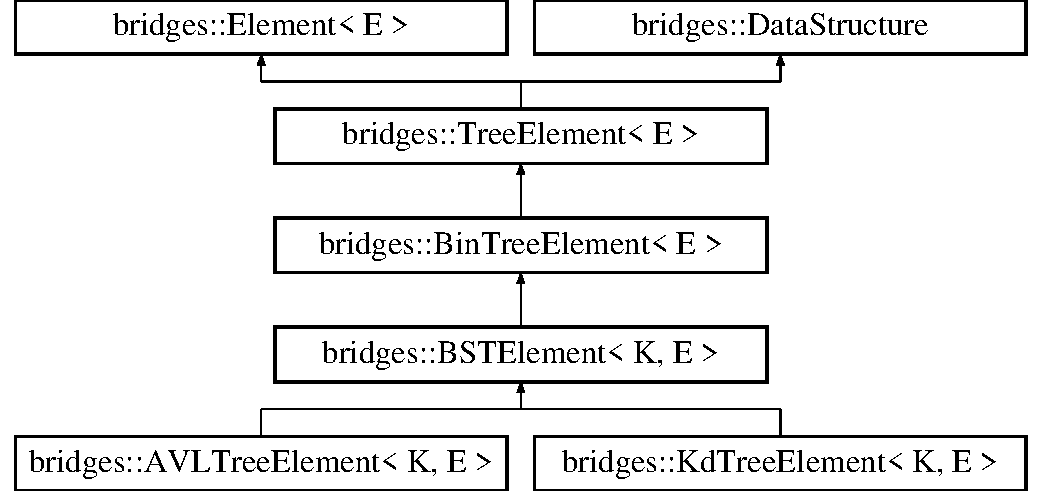
\includegraphics[height=5.000000cm]{classbridges_1_1_bin_tree_element}
\end{center}
\end{figure}
\subsection*{Public Member Functions}
\begin{DoxyCompactItemize}
\item 
\hyperlink{classbridges_1_1_bin_tree_element_a1c60db90bda9ecd3f5a61b5f33f49173}{Bin\+Tree\+Element} (\hyperlink{classbridges_1_1_bin_tree_element}{Bin\+Tree\+Element} $\ast$l, \hyperlink{classbridges_1_1_bin_tree_element}{Bin\+Tree\+Element} $\ast$r, const E \&e=E(), const string \&lab=string())
\item 
\hyperlink{classbridges_1_1_bin_tree_element_a37d12669e5bfe13ebf230dd8fd2a5816}{Bin\+Tree\+Element} (const E \&e=E(), const string \&lab=string())
\item 
virtual const string \hyperlink{classbridges_1_1_bin_tree_element_ae0bf807e8fd653574d161b4847c92e4e}{get\+D\+Stype} () const  override
\item 
virtual \hyperlink{classbridges_1_1_bin_tree_element}{Bin\+Tree\+Element} $\ast$ \hyperlink{classbridges_1_1_bin_tree_element_a8367ce9c4eea814637edc2c56efbde25}{get\+Left} ()
\item 
virtual const \hyperlink{classbridges_1_1_bin_tree_element}{Bin\+Tree\+Element} $\ast$ \hyperlink{classbridges_1_1_bin_tree_element_a04389903999ef5fe9cb22bdf63b61caa}{get\+Left} () const 
\item 
void \hyperlink{classbridges_1_1_bin_tree_element_a8f90f7f4c8da058ebfca64dd3728c50f}{set\+Left} (\hyperlink{classbridges_1_1_bin_tree_element}{Bin\+Tree\+Element} $\ast$l)
\item 
virtual \hyperlink{classbridges_1_1_bin_tree_element}{Bin\+Tree\+Element} $\ast$ \hyperlink{classbridges_1_1_bin_tree_element_a5751f2fe38e2364f68dc37939fce060f}{get\+Right} ()
\item 
virtual const \hyperlink{classbridges_1_1_bin_tree_element}{Bin\+Tree\+Element} $\ast$ \hyperlink{classbridges_1_1_bin_tree_element_af50af3f1ebc05439813b185fddfc131b}{get\+Right} () const 
\item 
void \hyperlink{classbridges_1_1_bin_tree_element_a0131f6ecefc7f68c6502d97292ea43bf}{set\+Right} (\hyperlink{classbridges_1_1_bin_tree_element}{Bin\+Tree\+Element} $\ast$r)
\end{DoxyCompactItemize}
\subsection*{Additional Inherited Members}


\subsection{Detailed Description}
\subsubsection*{template$<$typename E$>$class bridges\+::\+Bin\+Tree\+Element$<$ E $>$}

This class can be used to create binary tree elements, derived from \hyperlink{classbridges_1_1_tree_element}{Tree\+Element}. 

This class can be used to create binary tree elements, with left and right children.

Generic Parameters\+: E the application data type

\begin{DoxyAuthor}{Author}
Kalpathi Subramanian 
\end{DoxyAuthor}
\begin{DoxyDate}{Date}
6/12/15 
\end{DoxyDate}


\subsection{Constructor \& Destructor Documentation}
\hypertarget{classbridges_1_1_bin_tree_element_a1c60db90bda9ecd3f5a61b5f33f49173}{}\index{bridges\+::\+Bin\+Tree\+Element@{bridges\+::\+Bin\+Tree\+Element}!Bin\+Tree\+Element@{Bin\+Tree\+Element}}
\index{Bin\+Tree\+Element@{Bin\+Tree\+Element}!bridges\+::\+Bin\+Tree\+Element@{bridges\+::\+Bin\+Tree\+Element}}
\subsubsection[{Bin\+Tree\+Element(\+Bin\+Tree\+Element $\ast$l, Bin\+Tree\+Element $\ast$r, const E \&e=\+E(), const string \&lab=string())}]{\setlength{\rightskip}{0pt plus 5cm}template$<$typename E $>$ {\bf bridges\+::\+Bin\+Tree\+Element}$<$ E $>$\+::{\bf Bin\+Tree\+Element} (
\begin{DoxyParamCaption}
\item[{{\bf Bin\+Tree\+Element}$<$ E $>$ $\ast$}]{l, }
\item[{{\bf Bin\+Tree\+Element}$<$ E $>$ $\ast$}]{r, }
\item[{const E \&}]{e = {\ttfamily E()}, }
\item[{const string \&}]{lab = {\ttfamily string()}}
\end{DoxyParamCaption}
)\hspace{0.3cm}{\ttfamily [inline]}}\label{classbridges_1_1_bin_tree_element_a1c60db90bda9ecd3f5a61b5f33f49173}
Constructs a \hyperlink{classbridges_1_1_bin_tree_element}{Bin\+Tree\+Element} with the provided value, label, left and right Bin\+Tree\+Elements. The defaults will be used if not provided.


\begin{DoxyParams}{Parameters}
{\em val} & The data to hold \\
\hline
{\em lab} & The label to show \\
\hline
{\em l} & The left \hyperlink{classbridges_1_1_tree_element}{Tree\+Element} \\
\hline
{\em r} & The right \hyperlink{classbridges_1_1_tree_element}{Tree\+Element} \\
\hline
\end{DoxyParams}
\hypertarget{classbridges_1_1_bin_tree_element_a37d12669e5bfe13ebf230dd8fd2a5816}{}\index{bridges\+::\+Bin\+Tree\+Element@{bridges\+::\+Bin\+Tree\+Element}!Bin\+Tree\+Element@{Bin\+Tree\+Element}}
\index{Bin\+Tree\+Element@{Bin\+Tree\+Element}!bridges\+::\+Bin\+Tree\+Element@{bridges\+::\+Bin\+Tree\+Element}}
\subsubsection[{Bin\+Tree\+Element(const E \&e=\+E(), const string \&lab=string())}]{\setlength{\rightskip}{0pt plus 5cm}template$<$typename E $>$ {\bf bridges\+::\+Bin\+Tree\+Element}$<$ E $>$\+::{\bf Bin\+Tree\+Element} (
\begin{DoxyParamCaption}
\item[{const E \&}]{e = {\ttfamily E()}, }
\item[{const string \&}]{lab = {\ttfamily string()}}
\end{DoxyParamCaption}
)\hspace{0.3cm}{\ttfamily [inline]}}\label{classbridges_1_1_bin_tree_element_a37d12669e5bfe13ebf230dd8fd2a5816}
Constructs a \hyperlink{classbridges_1_1_bin_tree_element}{Bin\+Tree\+Element} with the provided value and label, setting the left and right \hyperlink{classbridges_1_1_bin_tree_element}{Bin\+Tree\+Element} to N\+U\+L\+L. The defaults will be used if not provided.


\begin{DoxyParams}{Parameters}
{\em val} & The data to hold \\
\hline
{\em lab} & The label to show \\
\hline
\end{DoxyParams}


\subsection{Member Function Documentation}
\hypertarget{classbridges_1_1_bin_tree_element_ae0bf807e8fd653574d161b4847c92e4e}{}\index{bridges\+::\+Bin\+Tree\+Element@{bridges\+::\+Bin\+Tree\+Element}!get\+D\+Stype@{get\+D\+Stype}}
\index{get\+D\+Stype@{get\+D\+Stype}!bridges\+::\+Bin\+Tree\+Element@{bridges\+::\+Bin\+Tree\+Element}}
\subsubsection[{get\+D\+Stype() const  override}]{\setlength{\rightskip}{0pt plus 5cm}template$<$typename E $>$ virtual const string {\bf bridges\+::\+Bin\+Tree\+Element}$<$ E $>$\+::get\+D\+Stype (
\begin{DoxyParamCaption}
{}
\end{DoxyParamCaption}
) const\hspace{0.3cm}{\ttfamily [inline]}, {\ttfamily [override]}, {\ttfamily [virtual]}}\label{classbridges_1_1_bin_tree_element_ae0bf807e8fd653574d161b4847c92e4e}
\begin{DoxyReturn}{Returns}
the data structure type 
\end{DoxyReturn}


Reimplemented from \hyperlink{classbridges_1_1_tree_element_a2990457495ddecc77fa1dda4f47f3010}{bridges\+::\+Tree\+Element$<$ E $>$}.



Reimplemented in \hyperlink{classbridges_1_1_kd_tree_element_a18326f2def8a9050e382949d70728cf0}{bridges\+::\+Kd\+Tree\+Element$<$ K, E $>$}, \hyperlink{classbridges_1_1_b_s_t_element_a56fdac281f5270446cf7ad98ff6c7a80}{bridges\+::\+B\+S\+T\+Element$<$ K, E $>$}, and \hyperlink{classbridges_1_1_a_v_l_tree_element_a408f7c79eb3414b54a8c9bdc6b31d972}{bridges\+::\+A\+V\+L\+Tree\+Element$<$ K, E $>$}.

\hypertarget{classbridges_1_1_bin_tree_element_a8367ce9c4eea814637edc2c56efbde25}{}\index{bridges\+::\+Bin\+Tree\+Element@{bridges\+::\+Bin\+Tree\+Element}!get\+Left@{get\+Left}}
\index{get\+Left@{get\+Left}!bridges\+::\+Bin\+Tree\+Element@{bridges\+::\+Bin\+Tree\+Element}}
\subsubsection[{get\+Left()}]{\setlength{\rightskip}{0pt plus 5cm}template$<$typename E $>$ virtual {\bf Bin\+Tree\+Element}$\ast$ {\bf bridges\+::\+Bin\+Tree\+Element}$<$ E $>$\+::get\+Left (
\begin{DoxyParamCaption}
{}
\end{DoxyParamCaption}
)\hspace{0.3cm}{\ttfamily [inline]}, {\ttfamily [virtual]}}\label{classbridges_1_1_bin_tree_element_a8367ce9c4eea814637edc2c56efbde25}
\begin{DoxyReturn}{Returns}
The left \hyperlink{classbridges_1_1_bin_tree_element}{Bin\+Tree\+Element} 
\end{DoxyReturn}


Reimplemented in \hyperlink{classbridges_1_1_kd_tree_element_ad7db63a4f82f5252c7e0809ac6486cb4}{bridges\+::\+Kd\+Tree\+Element$<$ K, E $>$}, \hyperlink{classbridges_1_1_b_s_t_element_a4d8987373c75b51fca94e3c0b78b87a6}{bridges\+::\+B\+S\+T\+Element$<$ K, E $>$}, and \hyperlink{classbridges_1_1_a_v_l_tree_element_a7b5d05660da127f5f6164120d9846d90}{bridges\+::\+A\+V\+L\+Tree\+Element$<$ K, E $>$}.

\hypertarget{classbridges_1_1_bin_tree_element_a04389903999ef5fe9cb22bdf63b61caa}{}\index{bridges\+::\+Bin\+Tree\+Element@{bridges\+::\+Bin\+Tree\+Element}!get\+Left@{get\+Left}}
\index{get\+Left@{get\+Left}!bridges\+::\+Bin\+Tree\+Element@{bridges\+::\+Bin\+Tree\+Element}}
\subsubsection[{get\+Left() const }]{\setlength{\rightskip}{0pt plus 5cm}template$<$typename E $>$ virtual const {\bf Bin\+Tree\+Element}$\ast$ {\bf bridges\+::\+Bin\+Tree\+Element}$<$ E $>$\+::get\+Left (
\begin{DoxyParamCaption}
{}
\end{DoxyParamCaption}
) const\hspace{0.3cm}{\ttfamily [inline]}, {\ttfamily [virtual]}}\label{classbridges_1_1_bin_tree_element_a04389903999ef5fe9cb22bdf63b61caa}
Constant version 

Reimplemented in \hyperlink{classbridges_1_1_kd_tree_element_a913d6c95eb6b5074710ebd1528861887}{bridges\+::\+Kd\+Tree\+Element$<$ K, E $>$}, \hyperlink{classbridges_1_1_b_s_t_element_a6dc35e175e993ebed845297264cfbc06}{bridges\+::\+B\+S\+T\+Element$<$ K, E $>$}, and \hyperlink{classbridges_1_1_a_v_l_tree_element_a4e1d2bd4430627ef759479b9fcf5c98b}{bridges\+::\+A\+V\+L\+Tree\+Element$<$ K, E $>$}.

\hypertarget{classbridges_1_1_bin_tree_element_a5751f2fe38e2364f68dc37939fce060f}{}\index{bridges\+::\+Bin\+Tree\+Element@{bridges\+::\+Bin\+Tree\+Element}!get\+Right@{get\+Right}}
\index{get\+Right@{get\+Right}!bridges\+::\+Bin\+Tree\+Element@{bridges\+::\+Bin\+Tree\+Element}}
\subsubsection[{get\+Right()}]{\setlength{\rightskip}{0pt plus 5cm}template$<$typename E $>$ virtual {\bf Bin\+Tree\+Element}$\ast$ {\bf bridges\+::\+Bin\+Tree\+Element}$<$ E $>$\+::get\+Right (
\begin{DoxyParamCaption}
{}
\end{DoxyParamCaption}
)\hspace{0.3cm}{\ttfamily [inline]}, {\ttfamily [virtual]}}\label{classbridges_1_1_bin_tree_element_a5751f2fe38e2364f68dc37939fce060f}
\begin{DoxyReturn}{Returns}
The right \hyperlink{classbridges_1_1_bin_tree_element}{Bin\+Tree\+Element} 
\end{DoxyReturn}


Reimplemented in \hyperlink{classbridges_1_1_kd_tree_element_a8e1090891a720231c2009d1d222471e9}{bridges\+::\+Kd\+Tree\+Element$<$ K, E $>$}, \hyperlink{classbridges_1_1_b_s_t_element_a35e93bce32de933522dccde5f2b5ffd9}{bridges\+::\+B\+S\+T\+Element$<$ K, E $>$}, and \hyperlink{classbridges_1_1_a_v_l_tree_element_a909b46ebf3e8c6a3434762a1f01499e2}{bridges\+::\+A\+V\+L\+Tree\+Element$<$ K, E $>$}.

\hypertarget{classbridges_1_1_bin_tree_element_af50af3f1ebc05439813b185fddfc131b}{}\index{bridges\+::\+Bin\+Tree\+Element@{bridges\+::\+Bin\+Tree\+Element}!get\+Right@{get\+Right}}
\index{get\+Right@{get\+Right}!bridges\+::\+Bin\+Tree\+Element@{bridges\+::\+Bin\+Tree\+Element}}
\subsubsection[{get\+Right() const }]{\setlength{\rightskip}{0pt plus 5cm}template$<$typename E $>$ virtual const {\bf Bin\+Tree\+Element}$\ast$ {\bf bridges\+::\+Bin\+Tree\+Element}$<$ E $>$\+::get\+Right (
\begin{DoxyParamCaption}
{}
\end{DoxyParamCaption}
) const\hspace{0.3cm}{\ttfamily [inline]}, {\ttfamily [virtual]}}\label{classbridges_1_1_bin_tree_element_af50af3f1ebc05439813b185fddfc131b}
Constant version 

Reimplemented in \hyperlink{classbridges_1_1_kd_tree_element_a0185d1d0ced0616387b7fae8ce81dde2}{bridges\+::\+Kd\+Tree\+Element$<$ K, E $>$}, \hyperlink{classbridges_1_1_b_s_t_element_af783aa676fe3fcbf4896f1dc21aabb9a}{bridges\+::\+B\+S\+T\+Element$<$ K, E $>$}, and \hyperlink{classbridges_1_1_a_v_l_tree_element_a45214b0f2d3b8acb78a5ce34333becd2}{bridges\+::\+A\+V\+L\+Tree\+Element$<$ K, E $>$}.

\hypertarget{classbridges_1_1_bin_tree_element_a8f90f7f4c8da058ebfca64dd3728c50f}{}\index{bridges\+::\+Bin\+Tree\+Element@{bridges\+::\+Bin\+Tree\+Element}!set\+Left@{set\+Left}}
\index{set\+Left@{set\+Left}!bridges\+::\+Bin\+Tree\+Element@{bridges\+::\+Bin\+Tree\+Element}}
\subsubsection[{set\+Left(\+Bin\+Tree\+Element $\ast$l)}]{\setlength{\rightskip}{0pt plus 5cm}template$<$typename E $>$ void {\bf bridges\+::\+Bin\+Tree\+Element}$<$ E $>$\+::set\+Left (
\begin{DoxyParamCaption}
\item[{{\bf Bin\+Tree\+Element}$<$ E $>$ $\ast$}]{l}
\end{DoxyParamCaption}
)\hspace{0.3cm}{\ttfamily [inline]}}\label{classbridges_1_1_bin_tree_element_a8f90f7f4c8da058ebfca64dd3728c50f}
Sets left to \char`\"{}l\char`\"{} 
\begin{DoxyParams}{Parameters}
{\em l} & The left \hyperlink{classbridges_1_1_bin_tree_element}{Bin\+Tree\+Element}\\
\hline
{\em l} & left child pointer \\
\hline
\end{DoxyParams}
\hypertarget{classbridges_1_1_bin_tree_element_a0131f6ecefc7f68c6502d97292ea43bf}{}\index{bridges\+::\+Bin\+Tree\+Element@{bridges\+::\+Bin\+Tree\+Element}!set\+Right@{set\+Right}}
\index{set\+Right@{set\+Right}!bridges\+::\+Bin\+Tree\+Element@{bridges\+::\+Bin\+Tree\+Element}}
\subsubsection[{set\+Right(\+Bin\+Tree\+Element $\ast$r)}]{\setlength{\rightskip}{0pt plus 5cm}template$<$typename E $>$ void {\bf bridges\+::\+Bin\+Tree\+Element}$<$ E $>$\+::set\+Right (
\begin{DoxyParamCaption}
\item[{{\bf Bin\+Tree\+Element}$<$ E $>$ $\ast$}]{r}
\end{DoxyParamCaption}
)\hspace{0.3cm}{\ttfamily [inline]}}\label{classbridges_1_1_bin_tree_element_a0131f6ecefc7f68c6502d97292ea43bf}
Sets right to \char`\"{}r\char`\"{} 
\begin{DoxyParams}{Parameters}
{\em r} & The right \hyperlink{classbridges_1_1_bin_tree_element}{Bin\+Tree\+Element}\\
\hline
{\em r} & right child pointer \\
\hline
\end{DoxyParams}


The documentation for this class was generated from the following file\+:\begin{DoxyCompactItemize}
\item 
/\+Users/krs/gr/bridges/bridges17/cxx/src/\hyperlink{_bin_tree_element_8h}{Bin\+Tree\+Element.\+h}\end{DoxyCompactItemize}

\hypertarget{classbridges_1_1_book}{}\section{bridges\+:\+:Book Class Reference}
\label{classbridges_1_1_book}\index{bridges\+::\+Book@{bridges\+::\+Book}}


A \mbox{\hyperlink{classbridges_1_1_book}{Book}} object, used along with the books data source.  




{\ttfamily \#include $<$Book.\+h$>$}

\subsection*{Public Member Functions}
\begin{DoxyCompactItemize}
\item 
\mbox{\hyperlink{classbridges_1_1_book_abb2903c640bd263a2e077d52e12a773e}{Book}} ()
\item 
\mbox{\hyperlink{classbridges_1_1_book_a4256eb5015b42e511d950c45103cef63}{Book}} (const string \&author\+Name, int author\+Birth, int author\+Death, const string \&title, const vector$<$ string $>$ \&lang, const vector$<$ string $>$ \&genre, const vector$<$ string $>$ \&subject, int num\+Chars, int num\+Words, int num\+Sentences, int num\+Difficult\+Words, const string \&url, int downloads)
\item 
string \mbox{\hyperlink{classbridges_1_1_book_a1f25d71b565a1bf5c82f76cce5dcc537}{get\+Author\+Name}} () const
\item 
void \mbox{\hyperlink{classbridges_1_1_book_a4ca756815b519a0a4d1ae5d3b21aa2d2}{set\+Author\+Name}} (const string \&author\+Name)
\item 
int \mbox{\hyperlink{classbridges_1_1_book_ac2c02b94f40eaddc7a2cca3f90976093}{get\+Author\+Birth}} () const
\item 
void \mbox{\hyperlink{classbridges_1_1_book_adca4d6766fa0068e23926ae95ed8411f}{set\+Author\+Birth}} (int author\+Birth)
\item 
int \mbox{\hyperlink{classbridges_1_1_book_a449e48d10878833b2f983deb993124dc}{get\+Author\+Death}} () const
\item 
void \mbox{\hyperlink{classbridges_1_1_book_a044ad1b1b6418d7545c6f957b2757bcd}{set\+Author\+Death}} (int author\+Death)
\item 
string \mbox{\hyperlink{classbridges_1_1_book_a5eda2e13c3b5523498d42845219eb175}{get\+Title}} () const
\item 
void \mbox{\hyperlink{classbridges_1_1_book_a68e4e04db8915b6baff809c46e6d1df9}{set\+Title}} (const string \&title)
\item 
vector$<$ string $>$ \mbox{\hyperlink{classbridges_1_1_book_a946923e7d93c552f699ef44a5bbed643}{get\+Lang}} () const
\item 
void \mbox{\hyperlink{classbridges_1_1_book_a7c96cf79f310f78eb16035c6874afa05}{set\+Lang}} (const vector$<$ string $>$ \&lang)
\item 
vector$<$ string $>$ \mbox{\hyperlink{classbridges_1_1_book_a5c7c8787f7dca4634980d657807a0b22}{get\+Genre}} () const
\item 
void \mbox{\hyperlink{classbridges_1_1_book_a3743b908548b944543af533b030a1eca}{set\+Genre}} (const vector$<$ string $>$ \&genre)
\item 
vector$<$ string $>$ \mbox{\hyperlink{classbridges_1_1_book_a95158e5538b78c2115a2102b33d56980}{get\+Subject}} () const
\item 
void \mbox{\hyperlink{classbridges_1_1_book_aff19a506929a6df5503e2cd3e293381e}{set\+Subject}} (const vector$<$ string $>$ \&subject)
\item 
string \mbox{\hyperlink{classbridges_1_1_book_a3facf86f7560e974ec7cd81e0fc58800}{get\+U\+RL}} () const
\item 
void \mbox{\hyperlink{classbridges_1_1_book_a48d590f296837b8eb9ac10451c83d23b}{set\+U\+RL}} (const string \&url)
\item 
int \mbox{\hyperlink{classbridges_1_1_book_a96343d553aeadefe8aa88da3e1e9e635}{get\+Num\+Chars}} () const
\item 
void \mbox{\hyperlink{classbridges_1_1_book_a31f85f174ab86e6f9eb2131c3dbe1cdf}{set\+Num\+Chars}} (int num\+Chars)
\item 
int \mbox{\hyperlink{classbridges_1_1_book_a8da8afb48552bcc8095829c2741aa22f}{get\+Num\+Words}} () const
\item 
void \mbox{\hyperlink{classbridges_1_1_book_acbed3f0ff253868d8747826a27ef30ac}{set\+Num\+Words}} (int num\+Words)
\item 
int \mbox{\hyperlink{classbridges_1_1_book_ab426149d54f152a6a8e67d75d9b37f25}{get\+Num\+Sentences}} () const
\item 
void \mbox{\hyperlink{classbridges_1_1_book_af16061c14c40b1672c7801a4c3a2d33b}{set\+Num\+Sentences}} (int num\+Sentences)
\item 
int \mbox{\hyperlink{classbridges_1_1_book_a6a2622b9eee31c4abd222282f72e641c}{get\+Num\+Difficult\+Words}} () const
\item 
void \mbox{\hyperlink{classbridges_1_1_book_adc7a54f2a494aeac02cadb3eb4caedbc}{set\+Num\+Difficult\+Words}} (int num\+Difficult\+Words)
\item 
int \mbox{\hyperlink{classbridges_1_1_book_a5cf7753a23c68de8703df2fab5b5193a}{get\+Downloads}} () const
\item 
void \mbox{\hyperlink{classbridges_1_1_book_aa3e894e59ae043e7271861772b03632c}{set\+Downloads}} (int downloads)
\end{DoxyCompactItemize}


\subsection{Detailed Description}
A \mbox{\hyperlink{classbridges_1_1_book}{Book}} object, used along with the books data source. 

This is a convenience class provided for users who wish to use this data source as part of their application. It provides an A\+PI that makes it easy to access the attributes of this data set.

Refer to tutorial examples to using this data source in data structure assignments.

\begin{DoxyAuthor}{Author}
Kalpathi Subramanian 
\end{DoxyAuthor}
\begin{DoxyDate}{Date}
1/16/17 
\end{DoxyDate}


\subsection{Constructor \& Destructor Documentation}
\mbox{\Hypertarget{classbridges_1_1_book_abb2903c640bd263a2e077d52e12a773e}\label{classbridges_1_1_book_abb2903c640bd263a2e077d52e12a773e}} 
\index{bridges\+::\+Book@{bridges\+::\+Book}!Book@{Book}}
\index{Book@{Book}!bridges\+::\+Book@{bridges\+::\+Book}}
\subsubsection{\texorpdfstring{Book()}{Book()}\hspace{0.1cm}{\footnotesize\ttfamily [1/2]}}
{\footnotesize\ttfamily bridges\+::\+Book\+::\+Book (\begin{DoxyParamCaption}{ }\end{DoxyParamCaption})\hspace{0.3cm}{\ttfamily [inline]}}

\mbox{\Hypertarget{classbridges_1_1_book_a4256eb5015b42e511d950c45103cef63}\label{classbridges_1_1_book_a4256eb5015b42e511d950c45103cef63}} 
\index{bridges\+::\+Book@{bridges\+::\+Book}!Book@{Book}}
\index{Book@{Book}!bridges\+::\+Book@{bridges\+::\+Book}}
\subsubsection{\texorpdfstring{Book()}{Book()}\hspace{0.1cm}{\footnotesize\ttfamily [2/2]}}
{\footnotesize\ttfamily bridges\+::\+Book\+::\+Book (\begin{DoxyParamCaption}\item[{const string \&}]{author\+Name,  }\item[{int}]{author\+Birth,  }\item[{int}]{author\+Death,  }\item[{const string \&}]{title,  }\item[{const vector$<$ string $>$ \&}]{lang,  }\item[{const vector$<$ string $>$ \&}]{genre,  }\item[{const vector$<$ string $>$ \&}]{subject,  }\item[{int}]{num\+Chars,  }\item[{int}]{num\+Words,  }\item[{int}]{num\+Sentences,  }\item[{int}]{num\+Difficult\+Words,  }\item[{const string \&}]{url,  }\item[{int}]{downloads }\end{DoxyParamCaption})\hspace{0.3cm}{\ttfamily [inline]}}



\subsection{Member Function Documentation}
\mbox{\Hypertarget{classbridges_1_1_book_ac2c02b94f40eaddc7a2cca3f90976093}\label{classbridges_1_1_book_ac2c02b94f40eaddc7a2cca3f90976093}} 
\index{bridges\+::\+Book@{bridges\+::\+Book}!get\+Author\+Birth@{get\+Author\+Birth}}
\index{get\+Author\+Birth@{get\+Author\+Birth}!bridges\+::\+Book@{bridges\+::\+Book}}
\subsubsection{\texorpdfstring{get\+Author\+Birth()}{getAuthorBirth()}}
{\footnotesize\ttfamily int bridges\+::\+Book\+::get\+Author\+Birth (\begin{DoxyParamCaption}{ }\end{DoxyParamCaption}) const\hspace{0.3cm}{\ttfamily [inline]}}

\mbox{\Hypertarget{classbridges_1_1_book_a449e48d10878833b2f983deb993124dc}\label{classbridges_1_1_book_a449e48d10878833b2f983deb993124dc}} 
\index{bridges\+::\+Book@{bridges\+::\+Book}!get\+Author\+Death@{get\+Author\+Death}}
\index{get\+Author\+Death@{get\+Author\+Death}!bridges\+::\+Book@{bridges\+::\+Book}}
\subsubsection{\texorpdfstring{get\+Author\+Death()}{getAuthorDeath()}}
{\footnotesize\ttfamily int bridges\+::\+Book\+::get\+Author\+Death (\begin{DoxyParamCaption}{ }\end{DoxyParamCaption}) const\hspace{0.3cm}{\ttfamily [inline]}}

\mbox{\Hypertarget{classbridges_1_1_book_a1f25d71b565a1bf5c82f76cce5dcc537}\label{classbridges_1_1_book_a1f25d71b565a1bf5c82f76cce5dcc537}} 
\index{bridges\+::\+Book@{bridges\+::\+Book}!get\+Author\+Name@{get\+Author\+Name}}
\index{get\+Author\+Name@{get\+Author\+Name}!bridges\+::\+Book@{bridges\+::\+Book}}
\subsubsection{\texorpdfstring{get\+Author\+Name()}{getAuthorName()}}
{\footnotesize\ttfamily string bridges\+::\+Book\+::get\+Author\+Name (\begin{DoxyParamCaption}{ }\end{DoxyParamCaption}) const\hspace{0.3cm}{\ttfamily [inline]}}

\mbox{\Hypertarget{classbridges_1_1_book_a5cf7753a23c68de8703df2fab5b5193a}\label{classbridges_1_1_book_a5cf7753a23c68de8703df2fab5b5193a}} 
\index{bridges\+::\+Book@{bridges\+::\+Book}!get\+Downloads@{get\+Downloads}}
\index{get\+Downloads@{get\+Downloads}!bridges\+::\+Book@{bridges\+::\+Book}}
\subsubsection{\texorpdfstring{get\+Downloads()}{getDownloads()}}
{\footnotesize\ttfamily int bridges\+::\+Book\+::get\+Downloads (\begin{DoxyParamCaption}{ }\end{DoxyParamCaption}) const\hspace{0.3cm}{\ttfamily [inline]}}

\mbox{\Hypertarget{classbridges_1_1_book_a5c7c8787f7dca4634980d657807a0b22}\label{classbridges_1_1_book_a5c7c8787f7dca4634980d657807a0b22}} 
\index{bridges\+::\+Book@{bridges\+::\+Book}!get\+Genre@{get\+Genre}}
\index{get\+Genre@{get\+Genre}!bridges\+::\+Book@{bridges\+::\+Book}}
\subsubsection{\texorpdfstring{get\+Genre()}{getGenre()}}
{\footnotesize\ttfamily vector$<$string$>$ bridges\+::\+Book\+::get\+Genre (\begin{DoxyParamCaption}{ }\end{DoxyParamCaption}) const\hspace{0.3cm}{\ttfamily [inline]}}

\mbox{\Hypertarget{classbridges_1_1_book_a946923e7d93c552f699ef44a5bbed643}\label{classbridges_1_1_book_a946923e7d93c552f699ef44a5bbed643}} 
\index{bridges\+::\+Book@{bridges\+::\+Book}!get\+Lang@{get\+Lang}}
\index{get\+Lang@{get\+Lang}!bridges\+::\+Book@{bridges\+::\+Book}}
\subsubsection{\texorpdfstring{get\+Lang()}{getLang()}}
{\footnotesize\ttfamily vector$<$string$>$ bridges\+::\+Book\+::get\+Lang (\begin{DoxyParamCaption}{ }\end{DoxyParamCaption}) const\hspace{0.3cm}{\ttfamily [inline]}}

\mbox{\Hypertarget{classbridges_1_1_book_a96343d553aeadefe8aa88da3e1e9e635}\label{classbridges_1_1_book_a96343d553aeadefe8aa88da3e1e9e635}} 
\index{bridges\+::\+Book@{bridges\+::\+Book}!get\+Num\+Chars@{get\+Num\+Chars}}
\index{get\+Num\+Chars@{get\+Num\+Chars}!bridges\+::\+Book@{bridges\+::\+Book}}
\subsubsection{\texorpdfstring{get\+Num\+Chars()}{getNumChars()}}
{\footnotesize\ttfamily int bridges\+::\+Book\+::get\+Num\+Chars (\begin{DoxyParamCaption}{ }\end{DoxyParamCaption}) const\hspace{0.3cm}{\ttfamily [inline]}}

\mbox{\Hypertarget{classbridges_1_1_book_a6a2622b9eee31c4abd222282f72e641c}\label{classbridges_1_1_book_a6a2622b9eee31c4abd222282f72e641c}} 
\index{bridges\+::\+Book@{bridges\+::\+Book}!get\+Num\+Difficult\+Words@{get\+Num\+Difficult\+Words}}
\index{get\+Num\+Difficult\+Words@{get\+Num\+Difficult\+Words}!bridges\+::\+Book@{bridges\+::\+Book}}
\subsubsection{\texorpdfstring{get\+Num\+Difficult\+Words()}{getNumDifficultWords()}}
{\footnotesize\ttfamily int bridges\+::\+Book\+::get\+Num\+Difficult\+Words (\begin{DoxyParamCaption}{ }\end{DoxyParamCaption}) const\hspace{0.3cm}{\ttfamily [inline]}}

\mbox{\Hypertarget{classbridges_1_1_book_ab426149d54f152a6a8e67d75d9b37f25}\label{classbridges_1_1_book_ab426149d54f152a6a8e67d75d9b37f25}} 
\index{bridges\+::\+Book@{bridges\+::\+Book}!get\+Num\+Sentences@{get\+Num\+Sentences}}
\index{get\+Num\+Sentences@{get\+Num\+Sentences}!bridges\+::\+Book@{bridges\+::\+Book}}
\subsubsection{\texorpdfstring{get\+Num\+Sentences()}{getNumSentences()}}
{\footnotesize\ttfamily int bridges\+::\+Book\+::get\+Num\+Sentences (\begin{DoxyParamCaption}{ }\end{DoxyParamCaption}) const\hspace{0.3cm}{\ttfamily [inline]}}

\mbox{\Hypertarget{classbridges_1_1_book_a8da8afb48552bcc8095829c2741aa22f}\label{classbridges_1_1_book_a8da8afb48552bcc8095829c2741aa22f}} 
\index{bridges\+::\+Book@{bridges\+::\+Book}!get\+Num\+Words@{get\+Num\+Words}}
\index{get\+Num\+Words@{get\+Num\+Words}!bridges\+::\+Book@{bridges\+::\+Book}}
\subsubsection{\texorpdfstring{get\+Num\+Words()}{getNumWords()}}
{\footnotesize\ttfamily int bridges\+::\+Book\+::get\+Num\+Words (\begin{DoxyParamCaption}{ }\end{DoxyParamCaption}) const\hspace{0.3cm}{\ttfamily [inline]}}

\mbox{\Hypertarget{classbridges_1_1_book_a95158e5538b78c2115a2102b33d56980}\label{classbridges_1_1_book_a95158e5538b78c2115a2102b33d56980}} 
\index{bridges\+::\+Book@{bridges\+::\+Book}!get\+Subject@{get\+Subject}}
\index{get\+Subject@{get\+Subject}!bridges\+::\+Book@{bridges\+::\+Book}}
\subsubsection{\texorpdfstring{get\+Subject()}{getSubject()}}
{\footnotesize\ttfamily vector$<$string$>$ bridges\+::\+Book\+::get\+Subject (\begin{DoxyParamCaption}{ }\end{DoxyParamCaption}) const\hspace{0.3cm}{\ttfamily [inline]}}

\mbox{\Hypertarget{classbridges_1_1_book_a5eda2e13c3b5523498d42845219eb175}\label{classbridges_1_1_book_a5eda2e13c3b5523498d42845219eb175}} 
\index{bridges\+::\+Book@{bridges\+::\+Book}!get\+Title@{get\+Title}}
\index{get\+Title@{get\+Title}!bridges\+::\+Book@{bridges\+::\+Book}}
\subsubsection{\texorpdfstring{get\+Title()}{getTitle()}}
{\footnotesize\ttfamily string bridges\+::\+Book\+::get\+Title (\begin{DoxyParamCaption}{ }\end{DoxyParamCaption}) const\hspace{0.3cm}{\ttfamily [inline]}}

\mbox{\Hypertarget{classbridges_1_1_book_a3facf86f7560e974ec7cd81e0fc58800}\label{classbridges_1_1_book_a3facf86f7560e974ec7cd81e0fc58800}} 
\index{bridges\+::\+Book@{bridges\+::\+Book}!get\+U\+RL@{get\+U\+RL}}
\index{get\+U\+RL@{get\+U\+RL}!bridges\+::\+Book@{bridges\+::\+Book}}
\subsubsection{\texorpdfstring{get\+U\+R\+L()}{getURL()}}
{\footnotesize\ttfamily string bridges\+::\+Book\+::get\+U\+RL (\begin{DoxyParamCaption}{ }\end{DoxyParamCaption}) const\hspace{0.3cm}{\ttfamily [inline]}}

\mbox{\Hypertarget{classbridges_1_1_book_adca4d6766fa0068e23926ae95ed8411f}\label{classbridges_1_1_book_adca4d6766fa0068e23926ae95ed8411f}} 
\index{bridges\+::\+Book@{bridges\+::\+Book}!set\+Author\+Birth@{set\+Author\+Birth}}
\index{set\+Author\+Birth@{set\+Author\+Birth}!bridges\+::\+Book@{bridges\+::\+Book}}
\subsubsection{\texorpdfstring{set\+Author\+Birth()}{setAuthorBirth()}}
{\footnotesize\ttfamily void bridges\+::\+Book\+::set\+Author\+Birth (\begin{DoxyParamCaption}\item[{int}]{author\+Birth }\end{DoxyParamCaption})\hspace{0.3cm}{\ttfamily [inline]}}

\mbox{\Hypertarget{classbridges_1_1_book_a044ad1b1b6418d7545c6f957b2757bcd}\label{classbridges_1_1_book_a044ad1b1b6418d7545c6f957b2757bcd}} 
\index{bridges\+::\+Book@{bridges\+::\+Book}!set\+Author\+Death@{set\+Author\+Death}}
\index{set\+Author\+Death@{set\+Author\+Death}!bridges\+::\+Book@{bridges\+::\+Book}}
\subsubsection{\texorpdfstring{set\+Author\+Death()}{setAuthorDeath()}}
{\footnotesize\ttfamily void bridges\+::\+Book\+::set\+Author\+Death (\begin{DoxyParamCaption}\item[{int}]{author\+Death }\end{DoxyParamCaption})\hspace{0.3cm}{\ttfamily [inline]}}

\mbox{\Hypertarget{classbridges_1_1_book_a4ca756815b519a0a4d1ae5d3b21aa2d2}\label{classbridges_1_1_book_a4ca756815b519a0a4d1ae5d3b21aa2d2}} 
\index{bridges\+::\+Book@{bridges\+::\+Book}!set\+Author\+Name@{set\+Author\+Name}}
\index{set\+Author\+Name@{set\+Author\+Name}!bridges\+::\+Book@{bridges\+::\+Book}}
\subsubsection{\texorpdfstring{set\+Author\+Name()}{setAuthorName()}}
{\footnotesize\ttfamily void bridges\+::\+Book\+::set\+Author\+Name (\begin{DoxyParamCaption}\item[{const string \&}]{author\+Name }\end{DoxyParamCaption})\hspace{0.3cm}{\ttfamily [inline]}}

\mbox{\Hypertarget{classbridges_1_1_book_aa3e894e59ae043e7271861772b03632c}\label{classbridges_1_1_book_aa3e894e59ae043e7271861772b03632c}} 
\index{bridges\+::\+Book@{bridges\+::\+Book}!set\+Downloads@{set\+Downloads}}
\index{set\+Downloads@{set\+Downloads}!bridges\+::\+Book@{bridges\+::\+Book}}
\subsubsection{\texorpdfstring{set\+Downloads()}{setDownloads()}}
{\footnotesize\ttfamily void bridges\+::\+Book\+::set\+Downloads (\begin{DoxyParamCaption}\item[{int}]{downloads }\end{DoxyParamCaption})\hspace{0.3cm}{\ttfamily [inline]}}

\mbox{\Hypertarget{classbridges_1_1_book_a3743b908548b944543af533b030a1eca}\label{classbridges_1_1_book_a3743b908548b944543af533b030a1eca}} 
\index{bridges\+::\+Book@{bridges\+::\+Book}!set\+Genre@{set\+Genre}}
\index{set\+Genre@{set\+Genre}!bridges\+::\+Book@{bridges\+::\+Book}}
\subsubsection{\texorpdfstring{set\+Genre()}{setGenre()}}
{\footnotesize\ttfamily void bridges\+::\+Book\+::set\+Genre (\begin{DoxyParamCaption}\item[{const vector$<$ string $>$ \&}]{genre }\end{DoxyParamCaption})\hspace{0.3cm}{\ttfamily [inline]}}

\mbox{\Hypertarget{classbridges_1_1_book_a7c96cf79f310f78eb16035c6874afa05}\label{classbridges_1_1_book_a7c96cf79f310f78eb16035c6874afa05}} 
\index{bridges\+::\+Book@{bridges\+::\+Book}!set\+Lang@{set\+Lang}}
\index{set\+Lang@{set\+Lang}!bridges\+::\+Book@{bridges\+::\+Book}}
\subsubsection{\texorpdfstring{set\+Lang()}{setLang()}}
{\footnotesize\ttfamily void bridges\+::\+Book\+::set\+Lang (\begin{DoxyParamCaption}\item[{const vector$<$ string $>$ \&}]{lang }\end{DoxyParamCaption})\hspace{0.3cm}{\ttfamily [inline]}}

\mbox{\Hypertarget{classbridges_1_1_book_a31f85f174ab86e6f9eb2131c3dbe1cdf}\label{classbridges_1_1_book_a31f85f174ab86e6f9eb2131c3dbe1cdf}} 
\index{bridges\+::\+Book@{bridges\+::\+Book}!set\+Num\+Chars@{set\+Num\+Chars}}
\index{set\+Num\+Chars@{set\+Num\+Chars}!bridges\+::\+Book@{bridges\+::\+Book}}
\subsubsection{\texorpdfstring{set\+Num\+Chars()}{setNumChars()}}
{\footnotesize\ttfamily void bridges\+::\+Book\+::set\+Num\+Chars (\begin{DoxyParamCaption}\item[{int}]{num\+Chars }\end{DoxyParamCaption})\hspace{0.3cm}{\ttfamily [inline]}}

\mbox{\Hypertarget{classbridges_1_1_book_adc7a54f2a494aeac02cadb3eb4caedbc}\label{classbridges_1_1_book_adc7a54f2a494aeac02cadb3eb4caedbc}} 
\index{bridges\+::\+Book@{bridges\+::\+Book}!set\+Num\+Difficult\+Words@{set\+Num\+Difficult\+Words}}
\index{set\+Num\+Difficult\+Words@{set\+Num\+Difficult\+Words}!bridges\+::\+Book@{bridges\+::\+Book}}
\subsubsection{\texorpdfstring{set\+Num\+Difficult\+Words()}{setNumDifficultWords()}}
{\footnotesize\ttfamily void bridges\+::\+Book\+::set\+Num\+Difficult\+Words (\begin{DoxyParamCaption}\item[{int}]{num\+Difficult\+Words }\end{DoxyParamCaption})\hspace{0.3cm}{\ttfamily [inline]}}

\mbox{\Hypertarget{classbridges_1_1_book_af16061c14c40b1672c7801a4c3a2d33b}\label{classbridges_1_1_book_af16061c14c40b1672c7801a4c3a2d33b}} 
\index{bridges\+::\+Book@{bridges\+::\+Book}!set\+Num\+Sentences@{set\+Num\+Sentences}}
\index{set\+Num\+Sentences@{set\+Num\+Sentences}!bridges\+::\+Book@{bridges\+::\+Book}}
\subsubsection{\texorpdfstring{set\+Num\+Sentences()}{setNumSentences()}}
{\footnotesize\ttfamily void bridges\+::\+Book\+::set\+Num\+Sentences (\begin{DoxyParamCaption}\item[{int}]{num\+Sentences }\end{DoxyParamCaption})\hspace{0.3cm}{\ttfamily [inline]}}

\mbox{\Hypertarget{classbridges_1_1_book_acbed3f0ff253868d8747826a27ef30ac}\label{classbridges_1_1_book_acbed3f0ff253868d8747826a27ef30ac}} 
\index{bridges\+::\+Book@{bridges\+::\+Book}!set\+Num\+Words@{set\+Num\+Words}}
\index{set\+Num\+Words@{set\+Num\+Words}!bridges\+::\+Book@{bridges\+::\+Book}}
\subsubsection{\texorpdfstring{set\+Num\+Words()}{setNumWords()}}
{\footnotesize\ttfamily void bridges\+::\+Book\+::set\+Num\+Words (\begin{DoxyParamCaption}\item[{int}]{num\+Words }\end{DoxyParamCaption})\hspace{0.3cm}{\ttfamily [inline]}}

\mbox{\Hypertarget{classbridges_1_1_book_aff19a506929a6df5503e2cd3e293381e}\label{classbridges_1_1_book_aff19a506929a6df5503e2cd3e293381e}} 
\index{bridges\+::\+Book@{bridges\+::\+Book}!set\+Subject@{set\+Subject}}
\index{set\+Subject@{set\+Subject}!bridges\+::\+Book@{bridges\+::\+Book}}
\subsubsection{\texorpdfstring{set\+Subject()}{setSubject()}}
{\footnotesize\ttfamily void bridges\+::\+Book\+::set\+Subject (\begin{DoxyParamCaption}\item[{const vector$<$ string $>$ \&}]{subject }\end{DoxyParamCaption})\hspace{0.3cm}{\ttfamily [inline]}}

\mbox{\Hypertarget{classbridges_1_1_book_a68e4e04db8915b6baff809c46e6d1df9}\label{classbridges_1_1_book_a68e4e04db8915b6baff809c46e6d1df9}} 
\index{bridges\+::\+Book@{bridges\+::\+Book}!set\+Title@{set\+Title}}
\index{set\+Title@{set\+Title}!bridges\+::\+Book@{bridges\+::\+Book}}
\subsubsection{\texorpdfstring{set\+Title()}{setTitle()}}
{\footnotesize\ttfamily void bridges\+::\+Book\+::set\+Title (\begin{DoxyParamCaption}\item[{const string \&}]{title }\end{DoxyParamCaption})\hspace{0.3cm}{\ttfamily [inline]}}

\mbox{\Hypertarget{classbridges_1_1_book_a48d590f296837b8eb9ac10451c83d23b}\label{classbridges_1_1_book_a48d590f296837b8eb9ac10451c83d23b}} 
\index{bridges\+::\+Book@{bridges\+::\+Book}!set\+U\+RL@{set\+U\+RL}}
\index{set\+U\+RL@{set\+U\+RL}!bridges\+::\+Book@{bridges\+::\+Book}}
\subsubsection{\texorpdfstring{set\+U\+R\+L()}{setURL()}}
{\footnotesize\ttfamily void bridges\+::\+Book\+::set\+U\+RL (\begin{DoxyParamCaption}\item[{const string \&}]{url }\end{DoxyParamCaption})\hspace{0.3cm}{\ttfamily [inline]}}



The documentation for this class was generated from the following file\+:\begin{DoxyCompactItemize}
\item 
/\+Users/kalpathi/gr/bridges/client/cxx/bridges17/src/data\+\_\+src/\mbox{\hyperlink{_book_8h}{Book.\+h}}\end{DoxyCompactItemize}

\hypertarget{classbridges_1_1_b_s_t_element}{}\section{bridges\+:\+:B\+S\+T\+Element$<$ K, E $>$ Class Template Reference}
\label{classbridges_1_1_b_s_t_element}\index{bridges\+::\+B\+S\+T\+Element$<$ K, E $>$@{bridges\+::\+B\+S\+T\+Element$<$ K, E $>$}}


This class can be used to create binary search tree elements, derived from \hyperlink{classbridges_1_1_bin_tree_element}{Bin\+Tree\+Element}.  




{\ttfamily \#include $<$B\+S\+T\+Element.\+h$>$}

Inheritance diagram for bridges\+:\+:B\+S\+T\+Element$<$ K, E $>$\+:\begin{figure}[H]
\begin{center}
\leavevmode
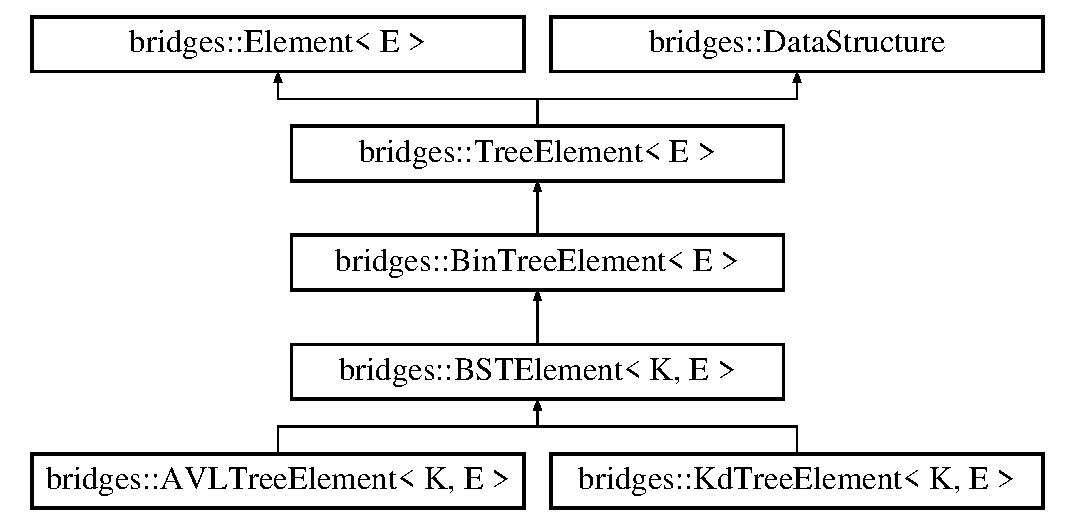
\includegraphics[height=5.000000cm]{classbridges_1_1_b_s_t_element}
\end{center}
\end{figure}
\subsection*{Public Member Functions}
\begin{DoxyCompactItemize}
\item 
\hyperlink{classbridges_1_1_b_s_t_element_aff7dbbb4011e85ea492d9a0c921895c5}{B\+S\+T\+Element} (const K \&k, \hyperlink{classbridges_1_1_b_s_t_element}{B\+S\+T\+Element} $\ast$l, \hyperlink{classbridges_1_1_b_s_t_element}{B\+S\+T\+Element} $\ast$r, const E \&val=E(), const string \&lab=string())
\item 
\hyperlink{classbridges_1_1_b_s_t_element_a13d32741606a8e3375b39f6dde99da5b}{B\+S\+T\+Element} (const K \&k, const E \&val=E(), const string \&lab=string())
\item 
virtual const string \hyperlink{classbridges_1_1_b_s_t_element_a56fdac281f5270446cf7ad98ff6c7a80}{get\+D\+Stype} () const  override
\item 
K \hyperlink{classbridges_1_1_b_s_t_element_ab418f627943fa76f36d13b196bff83b2}{get\+Key} () const 
\item 
void \hyperlink{classbridges_1_1_b_s_t_element_ae9edfa178c3b2d8bbaa7bd248bc469ce}{set\+Key} (const K \&k)
\item 
virtual \hyperlink{classbridges_1_1_b_s_t_element}{B\+S\+T\+Element} $\ast$ \hyperlink{classbridges_1_1_b_s_t_element_a4d8987373c75b51fca94e3c0b78b87a6}{get\+Left} () override
\item 
virtual const \hyperlink{classbridges_1_1_b_s_t_element}{B\+S\+T\+Element} $\ast$ \hyperlink{classbridges_1_1_b_s_t_element_a6dc35e175e993ebed845297264cfbc06}{get\+Left} () const  override
\item 
void \hyperlink{classbridges_1_1_b_s_t_element_a9bb5412bffab516268163ed772eb2c41}{set\+Left} (\hyperlink{classbridges_1_1_b_s_t_element}{B\+S\+T\+Element} $\ast$l)
\item 
virtual \hyperlink{classbridges_1_1_b_s_t_element}{B\+S\+T\+Element} $\ast$ \hyperlink{classbridges_1_1_b_s_t_element_a35e93bce32de933522dccde5f2b5ffd9}{get\+Right} () override
\item 
virtual const \hyperlink{classbridges_1_1_b_s_t_element}{B\+S\+T\+Element} $\ast$ \hyperlink{classbridges_1_1_b_s_t_element_af783aa676fe3fcbf4896f1dc21aabb9a}{get\+Right} () const  override
\item 
void \hyperlink{classbridges_1_1_b_s_t_element_a7267de974d13907f953afc78ea4fcd19}{set\+Right} (\hyperlink{classbridges_1_1_b_s_t_element}{B\+S\+T\+Element} $\ast$r)
\end{DoxyCompactItemize}
\subsection*{Protected Member Functions}
\begin{DoxyCompactItemize}
\item 
virtual const string \hyperlink{classbridges_1_1_b_s_t_element_afde56af31362642e6d65bf29f1b056d2}{get\+Element\+Representation} () const  override
\end{DoxyCompactItemize}
\subsection*{Protected Attributes}
\begin{DoxyCompactItemize}
\item 
K \hyperlink{classbridges_1_1_b_s_t_element_aebe8a0958484a0e28e777b423079bae2}{key} = K()
\end{DoxyCompactItemize}
\subsection*{Additional Inherited Members}


\subsection{Detailed Description}
\subsubsection*{template$<$typename K, typename E$>$class bridges\+::\+B\+S\+T\+Element$<$ K, E $>$}

This class can be used to create binary search tree elements, derived from \hyperlink{classbridges_1_1_bin_tree_element}{Bin\+Tree\+Element}. 

This class extends the \hyperlink{classbridges_1_1_bin_tree_element}{Bin\+Tree\+Element} class by adding a key property to allow for use in a binary search tree implementation.

Generic Parameters\+: K that is the search key type, E the application data type

\begin{DoxyAuthor}{Author}
Kalpathi Subramanian 
\end{DoxyAuthor}
\begin{DoxyDate}{Date}
6/18/15, 7/17/16 
\end{DoxyDate}


\subsection{Constructor \& Destructor Documentation}
\hypertarget{classbridges_1_1_b_s_t_element_aff7dbbb4011e85ea492d9a0c921895c5}{}\index{bridges\+::\+B\+S\+T\+Element@{bridges\+::\+B\+S\+T\+Element}!B\+S\+T\+Element@{B\+S\+T\+Element}}
\index{B\+S\+T\+Element@{B\+S\+T\+Element}!bridges\+::\+B\+S\+T\+Element@{bridges\+::\+B\+S\+T\+Element}}
\subsubsection[{B\+S\+T\+Element(const K \&k, B\+S\+T\+Element $\ast$l, B\+S\+T\+Element $\ast$r, const E \&val=\+E(), const string \&lab=string())}]{\setlength{\rightskip}{0pt plus 5cm}template$<$typename K , typename E $>$ {\bf bridges\+::\+B\+S\+T\+Element}$<$ K, E $>$\+::{\bf B\+S\+T\+Element} (
\begin{DoxyParamCaption}
\item[{const K \&}]{k, }
\item[{{\bf B\+S\+T\+Element}$<$ K, E $>$ $\ast$}]{l, }
\item[{{\bf B\+S\+T\+Element}$<$ K, E $>$ $\ast$}]{r, }
\item[{const E \&}]{val = {\ttfamily E()}, }
\item[{const string \&}]{lab = {\ttfamily string()}}
\end{DoxyParamCaption}
)\hspace{0.3cm}{\ttfamily [inline]}}\label{classbridges_1_1_b_s_t_element_aff7dbbb4011e85ea492d9a0c921895c5}
Constructs a \hyperlink{classbridges_1_1_b_s_t_element}{B\+S\+T\+Element} with the provided value, label, key, left and right B\+S\+T\+Elements. The defaults will be used if not provided.


\begin{DoxyParams}{Parameters}
{\em k} & The key for ordering \\
\hline
{\em val} & The data to hold \\
\hline
{\em lab} & The label to show \\
\hline
{\em l} & The left \hyperlink{classbridges_1_1_b_s_t_element}{B\+S\+T\+Element} \\
\hline
{\em r} & The right \hyperlink{classbridges_1_1_b_s_t_element}{B\+S\+T\+Element} \\
\hline
\end{DoxyParams}
\hypertarget{classbridges_1_1_b_s_t_element_a13d32741606a8e3375b39f6dde99da5b}{}\index{bridges\+::\+B\+S\+T\+Element@{bridges\+::\+B\+S\+T\+Element}!B\+S\+T\+Element@{B\+S\+T\+Element}}
\index{B\+S\+T\+Element@{B\+S\+T\+Element}!bridges\+::\+B\+S\+T\+Element@{bridges\+::\+B\+S\+T\+Element}}
\subsubsection[{B\+S\+T\+Element(const K \&k, const E \&val=\+E(), const string \&lab=string())}]{\setlength{\rightskip}{0pt plus 5cm}template$<$typename K , typename E $>$ {\bf bridges\+::\+B\+S\+T\+Element}$<$ K, E $>$\+::{\bf B\+S\+T\+Element} (
\begin{DoxyParamCaption}
\item[{const K \&}]{k, }
\item[{const E \&}]{val = {\ttfamily E()}, }
\item[{const string \&}]{lab = {\ttfamily string()}}
\end{DoxyParamCaption}
)\hspace{0.3cm}{\ttfamily [inline]}}\label{classbridges_1_1_b_s_t_element_a13d32741606a8e3375b39f6dde99da5b}
Constructs a \hyperlink{classbridges_1_1_b_s_t_element}{B\+S\+T\+Element} with the provided value, label, key, setting the left and right B\+S\+T\+Elements to N\+U\+L\+L. The defaults will be used if not provided.


\begin{DoxyParams}{Parameters}
{\em val} & The data to hold \\
\hline
{\em lab} & The label to show \\
\hline
{\em k} & The key for ordering \\
\hline
\end{DoxyParams}


\subsection{Member Function Documentation}
\hypertarget{classbridges_1_1_b_s_t_element_a56fdac281f5270446cf7ad98ff6c7a80}{}\index{bridges\+::\+B\+S\+T\+Element@{bridges\+::\+B\+S\+T\+Element}!get\+D\+Stype@{get\+D\+Stype}}
\index{get\+D\+Stype@{get\+D\+Stype}!bridges\+::\+B\+S\+T\+Element@{bridges\+::\+B\+S\+T\+Element}}
\subsubsection[{get\+D\+Stype() const  override}]{\setlength{\rightskip}{0pt plus 5cm}template$<$typename K , typename E $>$ virtual const string {\bf bridges\+::\+B\+S\+T\+Element}$<$ K, E $>$\+::get\+D\+Stype (
\begin{DoxyParamCaption}
{}
\end{DoxyParamCaption}
) const\hspace{0.3cm}{\ttfamily [inline]}, {\ttfamily [override]}, {\ttfamily [virtual]}}\label{classbridges_1_1_b_s_t_element_a56fdac281f5270446cf7ad98ff6c7a80}
\begin{DoxyReturn}{Returns}
the data structure type 
\end{DoxyReturn}


Reimplemented from \hyperlink{classbridges_1_1_bin_tree_element_ae0bf807e8fd653574d161b4847c92e4e}{bridges\+::\+Bin\+Tree\+Element$<$ E $>$}.



Reimplemented in \hyperlink{classbridges_1_1_kd_tree_element_a18326f2def8a9050e382949d70728cf0}{bridges\+::\+Kd\+Tree\+Element$<$ K, E $>$}, and \hyperlink{classbridges_1_1_a_v_l_tree_element_a408f7c79eb3414b54a8c9bdc6b31d972}{bridges\+::\+A\+V\+L\+Tree\+Element$<$ K, E $>$}.

\hypertarget{classbridges_1_1_b_s_t_element_afde56af31362642e6d65bf29f1b056d2}{}\index{bridges\+::\+B\+S\+T\+Element@{bridges\+::\+B\+S\+T\+Element}!get\+Element\+Representation@{get\+Element\+Representation}}
\index{get\+Element\+Representation@{get\+Element\+Representation}!bridges\+::\+B\+S\+T\+Element@{bridges\+::\+B\+S\+T\+Element}}
\subsubsection[{get\+Element\+Representation() const  override}]{\setlength{\rightskip}{0pt plus 5cm}template$<$typename K , typename E $>$ virtual const string {\bf bridges\+::\+B\+S\+T\+Element}$<$ K, E $>$\+::get\+Element\+Representation (
\begin{DoxyParamCaption}
{}
\end{DoxyParamCaption}
) const\hspace{0.3cm}{\ttfamily [inline]}, {\ttfamily [override]}, {\ttfamily [protected]}, {\ttfamily [virtual]}}\label{classbridges_1_1_b_s_t_element_afde56af31362642e6d65bf29f1b056d2}
\begin{DoxyReturn}{Returns}
The J\+S\+O\+N string of this element\textquotesingle{}s properties 
\end{DoxyReturn}


Reimplemented from \hyperlink{classbridges_1_1_element_aac13ea6244099496172c8549e48a9f73}{bridges\+::\+Element$<$ E $>$}.



Reimplemented in \hyperlink{classbridges_1_1_kd_tree_element_ab69079d403c51b31e2da02966f09615e}{bridges\+::\+Kd\+Tree\+Element$<$ K, E $>$}.

\hypertarget{classbridges_1_1_b_s_t_element_ab418f627943fa76f36d13b196bff83b2}{}\index{bridges\+::\+B\+S\+T\+Element@{bridges\+::\+B\+S\+T\+Element}!get\+Key@{get\+Key}}
\index{get\+Key@{get\+Key}!bridges\+::\+B\+S\+T\+Element@{bridges\+::\+B\+S\+T\+Element}}
\subsubsection[{get\+Key() const }]{\setlength{\rightskip}{0pt plus 5cm}template$<$typename K , typename E $>$ K {\bf bridges\+::\+B\+S\+T\+Element}$<$ K, E $>$\+::get\+Key (
\begin{DoxyParamCaption}
{}
\end{DoxyParamCaption}
) const\hspace{0.3cm}{\ttfamily [inline]}}\label{classbridges_1_1_b_s_t_element_ab418f627943fa76f36d13b196bff83b2}
\begin{DoxyReturn}{Returns}
The key of this \hyperlink{classbridges_1_1_b_s_t_element}{B\+S\+T\+Element} 
\end{DoxyReturn}
\hypertarget{classbridges_1_1_b_s_t_element_a4d8987373c75b51fca94e3c0b78b87a6}{}\index{bridges\+::\+B\+S\+T\+Element@{bridges\+::\+B\+S\+T\+Element}!get\+Left@{get\+Left}}
\index{get\+Left@{get\+Left}!bridges\+::\+B\+S\+T\+Element@{bridges\+::\+B\+S\+T\+Element}}
\subsubsection[{get\+Left() override}]{\setlength{\rightskip}{0pt plus 5cm}template$<$typename K , typename E $>$ virtual {\bf B\+S\+T\+Element}$\ast$ {\bf bridges\+::\+B\+S\+T\+Element}$<$ K, E $>$\+::get\+Left (
\begin{DoxyParamCaption}
{}
\end{DoxyParamCaption}
)\hspace{0.3cm}{\ttfamily [inline]}, {\ttfamily [override]}, {\ttfamily [virtual]}}\label{classbridges_1_1_b_s_t_element_a4d8987373c75b51fca94e3c0b78b87a6}
\begin{DoxyReturn}{Returns}
The left child 
\end{DoxyReturn}


Reimplemented from \hyperlink{classbridges_1_1_bin_tree_element_a8367ce9c4eea814637edc2c56efbde25}{bridges\+::\+Bin\+Tree\+Element$<$ E $>$}.



Reimplemented in \hyperlink{classbridges_1_1_kd_tree_element_ad7db63a4f82f5252c7e0809ac6486cb4}{bridges\+::\+Kd\+Tree\+Element$<$ K, E $>$}, and \hyperlink{classbridges_1_1_a_v_l_tree_element_a7b5d05660da127f5f6164120d9846d90}{bridges\+::\+A\+V\+L\+Tree\+Element$<$ K, E $>$}.

\hypertarget{classbridges_1_1_b_s_t_element_a6dc35e175e993ebed845297264cfbc06}{}\index{bridges\+::\+B\+S\+T\+Element@{bridges\+::\+B\+S\+T\+Element}!get\+Left@{get\+Left}}
\index{get\+Left@{get\+Left}!bridges\+::\+B\+S\+T\+Element@{bridges\+::\+B\+S\+T\+Element}}
\subsubsection[{get\+Left() const  override}]{\setlength{\rightskip}{0pt plus 5cm}template$<$typename K , typename E $>$ virtual const {\bf B\+S\+T\+Element}$\ast$ {\bf bridges\+::\+B\+S\+T\+Element}$<$ K, E $>$\+::get\+Left (
\begin{DoxyParamCaption}
{}
\end{DoxyParamCaption}
) const\hspace{0.3cm}{\ttfamily [inline]}, {\ttfamily [override]}, {\ttfamily [virtual]}}\label{classbridges_1_1_b_s_t_element_a6dc35e175e993ebed845297264cfbc06}
Constant version

\begin{DoxyReturn}{Returns}
The left child 
\end{DoxyReturn}


Reimplemented from \hyperlink{classbridges_1_1_bin_tree_element_a04389903999ef5fe9cb22bdf63b61caa}{bridges\+::\+Bin\+Tree\+Element$<$ E $>$}.



Reimplemented in \hyperlink{classbridges_1_1_kd_tree_element_a913d6c95eb6b5074710ebd1528861887}{bridges\+::\+Kd\+Tree\+Element$<$ K, E $>$}, and \hyperlink{classbridges_1_1_a_v_l_tree_element_a4e1d2bd4430627ef759479b9fcf5c98b}{bridges\+::\+A\+V\+L\+Tree\+Element$<$ K, E $>$}.

\hypertarget{classbridges_1_1_b_s_t_element_a35e93bce32de933522dccde5f2b5ffd9}{}\index{bridges\+::\+B\+S\+T\+Element@{bridges\+::\+B\+S\+T\+Element}!get\+Right@{get\+Right}}
\index{get\+Right@{get\+Right}!bridges\+::\+B\+S\+T\+Element@{bridges\+::\+B\+S\+T\+Element}}
\subsubsection[{get\+Right() override}]{\setlength{\rightskip}{0pt plus 5cm}template$<$typename K , typename E $>$ virtual {\bf B\+S\+T\+Element}$\ast$ {\bf bridges\+::\+B\+S\+T\+Element}$<$ K, E $>$\+::get\+Right (
\begin{DoxyParamCaption}
{}
\end{DoxyParamCaption}
)\hspace{0.3cm}{\ttfamily [inline]}, {\ttfamily [override]}, {\ttfamily [virtual]}}\label{classbridges_1_1_b_s_t_element_a35e93bce32de933522dccde5f2b5ffd9}
\begin{DoxyReturn}{Returns}
The right child 
\end{DoxyReturn}


Reimplemented from \hyperlink{classbridges_1_1_bin_tree_element_a5751f2fe38e2364f68dc37939fce060f}{bridges\+::\+Bin\+Tree\+Element$<$ E $>$}.



Reimplemented in \hyperlink{classbridges_1_1_kd_tree_element_a8e1090891a720231c2009d1d222471e9}{bridges\+::\+Kd\+Tree\+Element$<$ K, E $>$}, and \hyperlink{classbridges_1_1_a_v_l_tree_element_a909b46ebf3e8c6a3434762a1f01499e2}{bridges\+::\+A\+V\+L\+Tree\+Element$<$ K, E $>$}.

\hypertarget{classbridges_1_1_b_s_t_element_af783aa676fe3fcbf4896f1dc21aabb9a}{}\index{bridges\+::\+B\+S\+T\+Element@{bridges\+::\+B\+S\+T\+Element}!get\+Right@{get\+Right}}
\index{get\+Right@{get\+Right}!bridges\+::\+B\+S\+T\+Element@{bridges\+::\+B\+S\+T\+Element}}
\subsubsection[{get\+Right() const  override}]{\setlength{\rightskip}{0pt plus 5cm}template$<$typename K , typename E $>$ virtual const {\bf B\+S\+T\+Element}$\ast$ {\bf bridges\+::\+B\+S\+T\+Element}$<$ K, E $>$\+::get\+Right (
\begin{DoxyParamCaption}
{}
\end{DoxyParamCaption}
) const\hspace{0.3cm}{\ttfamily [inline]}, {\ttfamily [override]}, {\ttfamily [virtual]}}\label{classbridges_1_1_b_s_t_element_af783aa676fe3fcbf4896f1dc21aabb9a}
Constant version

\begin{DoxyReturn}{Returns}
The right child 
\end{DoxyReturn}


Reimplemented from \hyperlink{classbridges_1_1_bin_tree_element_af50af3f1ebc05439813b185fddfc131b}{bridges\+::\+Bin\+Tree\+Element$<$ E $>$}.



Reimplemented in \hyperlink{classbridges_1_1_kd_tree_element_a0185d1d0ced0616387b7fae8ce81dde2}{bridges\+::\+Kd\+Tree\+Element$<$ K, E $>$}, and \hyperlink{classbridges_1_1_a_v_l_tree_element_a45214b0f2d3b8acb78a5ce34333becd2}{bridges\+::\+A\+V\+L\+Tree\+Element$<$ K, E $>$}.

\hypertarget{classbridges_1_1_b_s_t_element_ae9edfa178c3b2d8bbaa7bd248bc469ce}{}\index{bridges\+::\+B\+S\+T\+Element@{bridges\+::\+B\+S\+T\+Element}!set\+Key@{set\+Key}}
\index{set\+Key@{set\+Key}!bridges\+::\+B\+S\+T\+Element@{bridges\+::\+B\+S\+T\+Element}}
\subsubsection[{set\+Key(const K \&k)}]{\setlength{\rightskip}{0pt plus 5cm}template$<$typename K , typename E $>$ void {\bf bridges\+::\+B\+S\+T\+Element}$<$ K, E $>$\+::set\+Key (
\begin{DoxyParamCaption}
\item[{const K \&}]{k}
\end{DoxyParamCaption}
)\hspace{0.3cm}{\ttfamily [inline]}}\label{classbridges_1_1_b_s_t_element_ae9edfa178c3b2d8bbaa7bd248bc469ce}
Set key to \char`\"{}k\char`\"{}


\begin{DoxyParams}{Parameters}
{\em k} & The key of this \hyperlink{classbridges_1_1_b_s_t_element}{B\+S\+T\+Element} \\
\hline
\end{DoxyParams}
\hypertarget{classbridges_1_1_b_s_t_element_a9bb5412bffab516268163ed772eb2c41}{}\index{bridges\+::\+B\+S\+T\+Element@{bridges\+::\+B\+S\+T\+Element}!set\+Left@{set\+Left}}
\index{set\+Left@{set\+Left}!bridges\+::\+B\+S\+T\+Element@{bridges\+::\+B\+S\+T\+Element}}
\subsubsection[{set\+Left(\+B\+S\+T\+Element $\ast$l)}]{\setlength{\rightskip}{0pt plus 5cm}template$<$typename K , typename E $>$ void {\bf bridges\+::\+B\+S\+T\+Element}$<$ K, E $>$\+::set\+Left (
\begin{DoxyParamCaption}
\item[{{\bf B\+S\+T\+Element}$<$ K, E $>$ $\ast$}]{l}
\end{DoxyParamCaption}
)\hspace{0.3cm}{\ttfamily [inline]}}\label{classbridges_1_1_b_s_t_element_a9bb5412bffab516268163ed772eb2c41}
Sets left to \char`\"{}l\char`\"{}


\begin{DoxyParams}{Parameters}
{\em l} & The left child \\
\hline
\end{DoxyParams}
\hypertarget{classbridges_1_1_b_s_t_element_a7267de974d13907f953afc78ea4fcd19}{}\index{bridges\+::\+B\+S\+T\+Element@{bridges\+::\+B\+S\+T\+Element}!set\+Right@{set\+Right}}
\index{set\+Right@{set\+Right}!bridges\+::\+B\+S\+T\+Element@{bridges\+::\+B\+S\+T\+Element}}
\subsubsection[{set\+Right(\+B\+S\+T\+Element $\ast$r)}]{\setlength{\rightskip}{0pt plus 5cm}template$<$typename K , typename E $>$ void {\bf bridges\+::\+B\+S\+T\+Element}$<$ K, E $>$\+::set\+Right (
\begin{DoxyParamCaption}
\item[{{\bf B\+S\+T\+Element}$<$ K, E $>$ $\ast$}]{r}
\end{DoxyParamCaption}
)\hspace{0.3cm}{\ttfamily [inline]}}\label{classbridges_1_1_b_s_t_element_a7267de974d13907f953afc78ea4fcd19}
Sets right to \char`\"{}r\char`\"{}


\begin{DoxyParams}{Parameters}
{\em r} & The right \hyperlink{classbridges_1_1_b_s_t_element}{B\+S\+T\+Element} \\
\hline
\end{DoxyParams}


\subsection{Member Data Documentation}
\hypertarget{classbridges_1_1_b_s_t_element_aebe8a0958484a0e28e777b423079bae2}{}\index{bridges\+::\+B\+S\+T\+Element@{bridges\+::\+B\+S\+T\+Element}!key@{key}}
\index{key@{key}!bridges\+::\+B\+S\+T\+Element@{bridges\+::\+B\+S\+T\+Element}}
\subsubsection[{key}]{\setlength{\rightskip}{0pt plus 5cm}template$<$typename K , typename E $>$ K {\bf bridges\+::\+B\+S\+T\+Element}$<$ K, E $>$\+::key = K()\hspace{0.3cm}{\ttfamily [protected]}}\label{classbridges_1_1_b_s_t_element_aebe8a0958484a0e28e777b423079bae2}


The documentation for this class was generated from the following file\+:\begin{DoxyCompactItemize}
\item 
/\+Users/krs/gr/bridges/client/cxx/src/\hyperlink{_b_s_t_element_8h}{B\+S\+T\+Element.\+h}\end{DoxyCompactItemize}

\hypertarget{classbridges_1_1_b_t_element}{}\section{bridges\+:\+:B\+T\+Element$<$ E $>$ Class Template Reference}
\label{classbridges_1_1_b_t_element}\index{bridges\+::\+B\+T\+Element$<$ E $>$@{bridges\+::\+B\+T\+Element$<$ E $>$}}


This class can be used to create binary tree elements, derived from \hyperlink{classbridges_1_1_tree_element}{Tree\+Element}.  




{\ttfamily \#include $<$B\+T\+Element.\+h$>$}

Inheritance diagram for bridges\+:\+:B\+T\+Element$<$ E $>$\+:\begin{figure}[H]
\begin{center}
\leavevmode
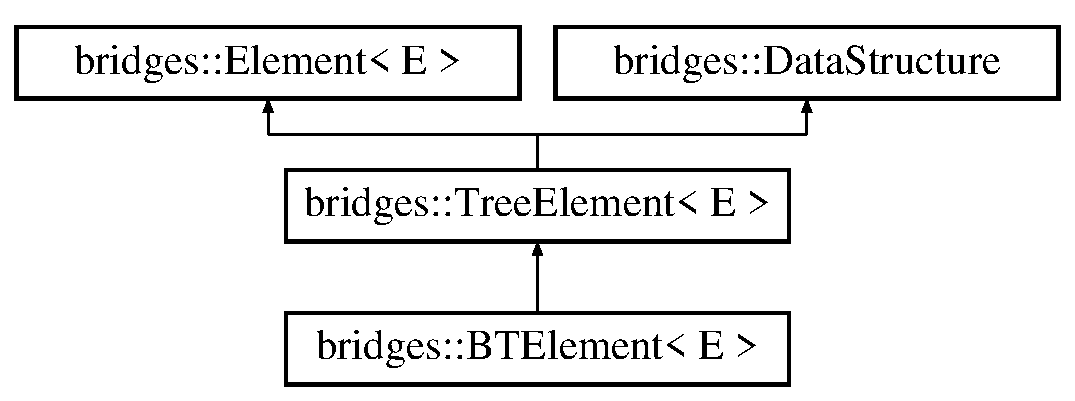
\includegraphics[height=2.470588cm]{classbridges_1_1_b_t_element}
\end{center}
\end{figure}
\subsection*{Public Member Functions}
\begin{DoxyCompactItemize}
\item 
\hyperlink{classbridges_1_1_b_t_element_a8abf38e5d2d70c247de6a6fe6b90bf1b}{B\+T\+Element} (\hyperlink{classbridges_1_1_b_t_element}{B\+T\+Element} $\ast$l, \hyperlink{classbridges_1_1_b_t_element}{B\+T\+Element} $\ast$r, const E \&e=E(), const string \&lab=string())
\item 
\hyperlink{classbridges_1_1_b_t_element_afdc1d11d1d65b23007334d337c279c3a}{B\+T\+Element} (const E \&e=E(), const string \&lab=string())
\item 
virtual const string \hyperlink{classbridges_1_1_b_t_element_ad5b614c00d40a703be0e5a89f92df7c7}{get\+D\+Stype} () const  override
\item 
virtual \hyperlink{classbridges_1_1_b_t_element}{B\+T\+Element} $\ast$ \hyperlink{classbridges_1_1_b_t_element_ab5955c2611b6ae8c3c48508e3e983f87}{get\+Left} ()
\item 
virtual const \hyperlink{classbridges_1_1_b_t_element}{B\+T\+Element} $\ast$ \hyperlink{classbridges_1_1_b_t_element_a8f4783c03397db330cce37b3592a31ce}{get\+Left} () const 
\item 
void \hyperlink{classbridges_1_1_b_t_element_a86f58ed6311eeb7eddc76188c423781c}{set\+Left} (\hyperlink{classbridges_1_1_b_t_element}{B\+T\+Element} $\ast$l)
\item 
virtual \hyperlink{classbridges_1_1_b_t_element}{B\+T\+Element} $\ast$ \hyperlink{classbridges_1_1_b_t_element_a931de8a71c04479a4aa0885ecee2a855}{get\+Right} ()
\item 
virtual const \hyperlink{classbridges_1_1_b_t_element}{B\+T\+Element} $\ast$ \hyperlink{classbridges_1_1_b_t_element_a08b04d11b921dde0db7c5e20961d0e2d}{get\+Right} () const 
\item 
void \hyperlink{classbridges_1_1_b_t_element_a19cf1ad19b8dd33e0539d77ed7f5c7f6}{set\+Right} (\hyperlink{classbridges_1_1_b_t_element}{B\+T\+Element} $\ast$r)
\end{DoxyCompactItemize}
\subsection*{Additional Inherited Members}


\subsection{Detailed Description}
\subsubsection*{template$<$typename E$>$class bridges\+::\+B\+T\+Element$<$ E $>$}

This class can be used to create binary tree elements, derived from \hyperlink{classbridges_1_1_tree_element}{Tree\+Element}. 

This class can be used to create binary tree elements, with left and right subtrees

Generic Parameters\+: E the application data type

\begin{DoxyAuthor}{Author}
Kalpathi Subramanian 
\end{DoxyAuthor}
\begin{DoxyDate}{Date}
6/12/15 
\end{DoxyDate}


\subsection{Constructor \& Destructor Documentation}
\hypertarget{classbridges_1_1_b_t_element_a8abf38e5d2d70c247de6a6fe6b90bf1b}{}\index{bridges\+::\+B\+T\+Element@{bridges\+::\+B\+T\+Element}!B\+T\+Element@{B\+T\+Element}}
\index{B\+T\+Element@{B\+T\+Element}!bridges\+::\+B\+T\+Element@{bridges\+::\+B\+T\+Element}}
\subsubsection[{B\+T\+Element(\+B\+T\+Element $\ast$l, B\+T\+Element $\ast$r, const E \&e=\+E(), const string \&lab=string())}]{\setlength{\rightskip}{0pt plus 5cm}template$<$typename E $>$ {\bf bridges\+::\+B\+T\+Element}$<$ E $>$\+::{\bf B\+T\+Element} (
\begin{DoxyParamCaption}
\item[{{\bf B\+T\+Element}$<$ E $>$ $\ast$}]{l, }
\item[{{\bf B\+T\+Element}$<$ E $>$ $\ast$}]{r, }
\item[{const E \&}]{e = {\ttfamily E()}, }
\item[{const string \&}]{lab = {\ttfamily string()}}
\end{DoxyParamCaption}
)\hspace{0.3cm}{\ttfamily [inline]}}\label{classbridges_1_1_b_t_element_a8abf38e5d2d70c247de6a6fe6b90bf1b}
Constructs a \hyperlink{classbridges_1_1_b_t_element}{B\+T\+Element} with the provided value, label, left and right B\+T\+Elements. The defaults will be used if not provided.


\begin{DoxyParams}{Parameters}
{\em val} & The data to hold \\
\hline
{\em lab} & The label to show \\
\hline
{\em l} & The left \hyperlink{classbridges_1_1_tree_element}{Tree\+Element} \\
\hline
{\em r} & The right \hyperlink{classbridges_1_1_tree_element}{Tree\+Element} \\
\hline
\end{DoxyParams}
\hypertarget{classbridges_1_1_b_t_element_afdc1d11d1d65b23007334d337c279c3a}{}\index{bridges\+::\+B\+T\+Element@{bridges\+::\+B\+T\+Element}!B\+T\+Element@{B\+T\+Element}}
\index{B\+T\+Element@{B\+T\+Element}!bridges\+::\+B\+T\+Element@{bridges\+::\+B\+T\+Element}}
\subsubsection[{B\+T\+Element(const E \&e=\+E(), const string \&lab=string())}]{\setlength{\rightskip}{0pt plus 5cm}template$<$typename E $>$ {\bf bridges\+::\+B\+T\+Element}$<$ E $>$\+::{\bf B\+T\+Element} (
\begin{DoxyParamCaption}
\item[{const E \&}]{e = {\ttfamily E()}, }
\item[{const string \&}]{lab = {\ttfamily string()}}
\end{DoxyParamCaption}
)\hspace{0.3cm}{\ttfamily [inline]}}\label{classbridges_1_1_b_t_element_afdc1d11d1d65b23007334d337c279c3a}
Constructs a \hyperlink{classbridges_1_1_b_t_element}{B\+T\+Element} with the provided value and label, setting the left and right \hyperlink{classbridges_1_1_b_t_element}{B\+T\+Element} to N\+U\+L\+L. The defaults will be used if not provided.


\begin{DoxyParams}{Parameters}
{\em val} & The data to hold \\
\hline
{\em lab} & The label to show \\
\hline
\end{DoxyParams}


\subsection{Member Function Documentation}
\hypertarget{classbridges_1_1_b_t_element_ad5b614c00d40a703be0e5a89f92df7c7}{}\index{bridges\+::\+B\+T\+Element@{bridges\+::\+B\+T\+Element}!get\+D\+Stype@{get\+D\+Stype}}
\index{get\+D\+Stype@{get\+D\+Stype}!bridges\+::\+B\+T\+Element@{bridges\+::\+B\+T\+Element}}
\subsubsection[{get\+D\+Stype() const  override}]{\setlength{\rightskip}{0pt plus 5cm}template$<$typename E $>$ virtual const string {\bf bridges\+::\+B\+T\+Element}$<$ E $>$\+::get\+D\+Stype (
\begin{DoxyParamCaption}
{}
\end{DoxyParamCaption}
) const\hspace{0.3cm}{\ttfamily [inline]}, {\ttfamily [override]}, {\ttfamily [virtual]}}\label{classbridges_1_1_b_t_element_ad5b614c00d40a703be0e5a89f92df7c7}
\begin{DoxyReturn}{Returns}
the data structure type 
\end{DoxyReturn}


Reimplemented from \hyperlink{classbridges_1_1_tree_element_a2990457495ddecc77fa1dda4f47f3010}{bridges\+::\+Tree\+Element$<$ E $>$}.

\hypertarget{classbridges_1_1_b_t_element_ab5955c2611b6ae8c3c48508e3e983f87}{}\index{bridges\+::\+B\+T\+Element@{bridges\+::\+B\+T\+Element}!get\+Left@{get\+Left}}
\index{get\+Left@{get\+Left}!bridges\+::\+B\+T\+Element@{bridges\+::\+B\+T\+Element}}
\subsubsection[{get\+Left()}]{\setlength{\rightskip}{0pt plus 5cm}template$<$typename E $>$ virtual {\bf B\+T\+Element}$\ast$ {\bf bridges\+::\+B\+T\+Element}$<$ E $>$\+::get\+Left (
\begin{DoxyParamCaption}
{}
\end{DoxyParamCaption}
)\hspace{0.3cm}{\ttfamily [inline]}, {\ttfamily [virtual]}}\label{classbridges_1_1_b_t_element_ab5955c2611b6ae8c3c48508e3e983f87}
\begin{DoxyReturn}{Returns}
The left \hyperlink{classbridges_1_1_b_t_element}{B\+T\+Element} 
\end{DoxyReturn}
\hypertarget{classbridges_1_1_b_t_element_a8f4783c03397db330cce37b3592a31ce}{}\index{bridges\+::\+B\+T\+Element@{bridges\+::\+B\+T\+Element}!get\+Left@{get\+Left}}
\index{get\+Left@{get\+Left}!bridges\+::\+B\+T\+Element@{bridges\+::\+B\+T\+Element}}
\subsubsection[{get\+Left() const }]{\setlength{\rightskip}{0pt plus 5cm}template$<$typename E $>$ virtual const {\bf B\+T\+Element}$\ast$ {\bf bridges\+::\+B\+T\+Element}$<$ E $>$\+::get\+Left (
\begin{DoxyParamCaption}
{}
\end{DoxyParamCaption}
) const\hspace{0.3cm}{\ttfamily [inline]}, {\ttfamily [virtual]}}\label{classbridges_1_1_b_t_element_a8f4783c03397db330cce37b3592a31ce}
Constant version \hypertarget{classbridges_1_1_b_t_element_a931de8a71c04479a4aa0885ecee2a855}{}\index{bridges\+::\+B\+T\+Element@{bridges\+::\+B\+T\+Element}!get\+Right@{get\+Right}}
\index{get\+Right@{get\+Right}!bridges\+::\+B\+T\+Element@{bridges\+::\+B\+T\+Element}}
\subsubsection[{get\+Right()}]{\setlength{\rightskip}{0pt plus 5cm}template$<$typename E $>$ virtual {\bf B\+T\+Element}$\ast$ {\bf bridges\+::\+B\+T\+Element}$<$ E $>$\+::get\+Right (
\begin{DoxyParamCaption}
{}
\end{DoxyParamCaption}
)\hspace{0.3cm}{\ttfamily [inline]}, {\ttfamily [virtual]}}\label{classbridges_1_1_b_t_element_a931de8a71c04479a4aa0885ecee2a855}
\begin{DoxyReturn}{Returns}
The right \hyperlink{classbridges_1_1_b_t_element}{B\+T\+Element} 
\end{DoxyReturn}
\hypertarget{classbridges_1_1_b_t_element_a08b04d11b921dde0db7c5e20961d0e2d}{}\index{bridges\+::\+B\+T\+Element@{bridges\+::\+B\+T\+Element}!get\+Right@{get\+Right}}
\index{get\+Right@{get\+Right}!bridges\+::\+B\+T\+Element@{bridges\+::\+B\+T\+Element}}
\subsubsection[{get\+Right() const }]{\setlength{\rightskip}{0pt plus 5cm}template$<$typename E $>$ virtual const {\bf B\+T\+Element}$\ast$ {\bf bridges\+::\+B\+T\+Element}$<$ E $>$\+::get\+Right (
\begin{DoxyParamCaption}
{}
\end{DoxyParamCaption}
) const\hspace{0.3cm}{\ttfamily [inline]}, {\ttfamily [virtual]}}\label{classbridges_1_1_b_t_element_a08b04d11b921dde0db7c5e20961d0e2d}
Constant version \hypertarget{classbridges_1_1_b_t_element_a86f58ed6311eeb7eddc76188c423781c}{}\index{bridges\+::\+B\+T\+Element@{bridges\+::\+B\+T\+Element}!set\+Left@{set\+Left}}
\index{set\+Left@{set\+Left}!bridges\+::\+B\+T\+Element@{bridges\+::\+B\+T\+Element}}
\subsubsection[{set\+Left(\+B\+T\+Element $\ast$l)}]{\setlength{\rightskip}{0pt plus 5cm}template$<$typename E $>$ void {\bf bridges\+::\+B\+T\+Element}$<$ E $>$\+::set\+Left (
\begin{DoxyParamCaption}
\item[{{\bf B\+T\+Element}$<$ E $>$ $\ast$}]{l}
\end{DoxyParamCaption}
)\hspace{0.3cm}{\ttfamily [inline]}}\label{classbridges_1_1_b_t_element_a86f58ed6311eeb7eddc76188c423781c}
Sets left to \char`\"{}l\char`\"{} 
\begin{DoxyParams}{Parameters}
{\em l} & The left \hyperlink{classbridges_1_1_b_t_element}{B\+T\+Element} \\
\hline
\end{DoxyParams}
\hypertarget{classbridges_1_1_b_t_element_a19cf1ad19b8dd33e0539d77ed7f5c7f6}{}\index{bridges\+::\+B\+T\+Element@{bridges\+::\+B\+T\+Element}!set\+Right@{set\+Right}}
\index{set\+Right@{set\+Right}!bridges\+::\+B\+T\+Element@{bridges\+::\+B\+T\+Element}}
\subsubsection[{set\+Right(\+B\+T\+Element $\ast$r)}]{\setlength{\rightskip}{0pt plus 5cm}template$<$typename E $>$ void {\bf bridges\+::\+B\+T\+Element}$<$ E $>$\+::set\+Right (
\begin{DoxyParamCaption}
\item[{{\bf B\+T\+Element}$<$ E $>$ $\ast$}]{r}
\end{DoxyParamCaption}
)\hspace{0.3cm}{\ttfamily [inline]}}\label{classbridges_1_1_b_t_element_a19cf1ad19b8dd33e0539d77ed7f5c7f6}
Sets right to \char`\"{}r\char`\"{} 
\begin{DoxyParams}{Parameters}
{\em r} & The right \hyperlink{classbridges_1_1_b_t_element}{B\+T\+Element} \\
\hline
\end{DoxyParams}


The documentation for this class was generated from the following file\+:\begin{DoxyCompactItemize}
\item 
/\+Users/krs/gr/bridges/bridges17/cxx/src/\hyperlink{_b_t_element_8h}{B\+T\+Element.\+h}\end{DoxyCompactItemize}

\hypertarget{classbridges_1_1_cancer_incidence}{}\section{bridges\+:\+:Cancer\+Incidence Class Reference}
\label{classbridges_1_1_cancer_incidence}\index{bridges\+::\+Cancer\+Incidence@{bridges\+::\+Cancer\+Incidence}}


A class representing the attributes for cancer incidence.  




{\ttfamily \#include $<$Cancer\+Incidence.\+h$>$}

\subsection*{Public Member Functions}
\begin{DoxyCompactItemize}
\item 
\hyperlink{classbridges_1_1_cancer_incidence_a3f5bb34394a22169bb4465c07e50fba1}{Cancer\+Incidence} ()
\item 
double \hyperlink{classbridges_1_1_cancer_incidence_a2b617c7ab02274e12078a93e0db35dc9}{get\+Age\+Adjusted\+Rate} () const 
\item 
void \hyperlink{classbridges_1_1_cancer_incidence_a607a50050fdfb75a737a684096046abf}{set\+Age\+Adjusted\+Rate} (double aar)
\item 
double \hyperlink{classbridges_1_1_cancer_incidence_ac9988f8726aa8ec864ded5211ef6a0c1}{get\+Age\+Adjusted\+C\+I\+\_\+\+Lower} () const 
\item 
void \hyperlink{classbridges_1_1_cancer_incidence_abc134f9f2c6d2be070ac8af502cfc10d}{set\+Age\+Adjusted\+C\+I\+\_\+\+Lower} (double ci\+\_\+l)
\item 
double \hyperlink{classbridges_1_1_cancer_incidence_a33dc94207eb04a43892a8a58d4b76c1a}{get\+Age\+Adjusted\+C\+I\+\_\+\+Upper} () const 
\item 
void \hyperlink{classbridges_1_1_cancer_incidence_abd120d1ca536223aa41f25de79eef31d}{set\+Age\+Adjusted\+C\+I\+\_\+\+Upper} (double ci\+\_\+u)
\item 
double \hyperlink{classbridges_1_1_cancer_incidence_aa8e67e9f1c7a8926642782cac762a7b8}{get\+Crude\+Rate} () const 
\item 
void \hyperlink{classbridges_1_1_cancer_incidence_af7b204185967ae857ef6fae9c0f70450}{set\+Crude\+Rate} (double cr)
\item 
double \hyperlink{classbridges_1_1_cancer_incidence_a7d35c53ce6f5876b30bca3334dac6c3c}{get\+Crude\+Rate\+\_\+\+C\+I\+\_\+\+Lower} () const 
\item 
void \hyperlink{classbridges_1_1_cancer_incidence_a58cdb11fa6e8d2766d3ef98b1e8aea1f}{set\+Crude\+Rate\+\_\+\+C\+I\+\_\+\+Lower} (double cr\+\_\+l)
\item 
double \hyperlink{classbridges_1_1_cancer_incidence_a0279f67ef72c3b175b2826c95ad40fe7}{get\+Crude\+Rate\+\_\+\+C\+I\+\_\+\+Upper} () const 
\item 
void \hyperlink{classbridges_1_1_cancer_incidence_a40d654a767d9b20ffa6931591d96d42a}{set\+Crude\+Rate\+\_\+\+C\+I\+\_\+\+Upper} (double cr\+\_\+u)
\item 
int \hyperlink{classbridges_1_1_cancer_incidence_ac2bd1a22a450657f2bd66b4d396bbba7}{get\+Year} () const 
\item 
void \hyperlink{classbridges_1_1_cancer_incidence_ac4c0d949ebb21dd890afe2714962fa5a}{set\+Year} (int y)
\item 
string \hyperlink{classbridges_1_1_cancer_incidence_af6105f18be298edff9b29b73bc3e1c81}{get\+Gender} () const 
\item 
void \hyperlink{classbridges_1_1_cancer_incidence_ad4b8d6d3b226567f60af07fa8e5d21ae}{set\+Gender} (const string \&g)
\item 
string \hyperlink{classbridges_1_1_cancer_incidence_a6e3850afa2162bee89ab5b8fa8462ddc}{get\+Race} () const 
\item 
void \hyperlink{classbridges_1_1_cancer_incidence_ae7cfd7532ab68ad521cc41d5172fd006}{set\+Race} (const string \&r)
\item 
string \hyperlink{classbridges_1_1_cancer_incidence_a14696225e64e30c88415f9436ec9c0ac}{get\+Event\+Type} () const 
\item 
void \hyperlink{classbridges_1_1_cancer_incidence_af17d0ebdf1a67834947e9cf5828c8fe3}{set\+Event\+Type} (const string \&et)
\item 
int \hyperlink{classbridges_1_1_cancer_incidence_a1667cd51355846ea7a746d120a7749f1}{get\+Population} () const 
\item 
void \hyperlink{classbridges_1_1_cancer_incidence_aaade0295abaeeabb23b9e03d5ffd364a}{set\+Population} (int pop)
\item 
string \hyperlink{classbridges_1_1_cancer_incidence_a0e64c2b77342aa72bcd0a460a9b994e0}{get\+Affected\+Area} () const 
\item 
void \hyperlink{classbridges_1_1_cancer_incidence_a4fc0d4133af2fef77b6b43c0d54f0e14}{set\+Affected\+Area} (const string \&area)
\item 
int \hyperlink{classbridges_1_1_cancer_incidence_a9d75ff868d631db828ad2eb22f6f90b4}{get\+Count} () const 
\item 
void \hyperlink{classbridges_1_1_cancer_incidence_a5fd30ffcf94f61cbca49112332ae4e94}{set\+Count} (int c)
\item 
double \hyperlink{classbridges_1_1_cancer_incidence_abbc7a6a2c9c9712a9a212279ec4ec535}{get\+Location\+X} () const 
\item 
void \hyperlink{classbridges_1_1_cancer_incidence_a6f7ec674c626e932378f01e08178d1fb}{set\+Location\+X} (double loc\+X)
\item 
double \hyperlink{classbridges_1_1_cancer_incidence_af31eb79fb63d4dab30b882b73d35fdf6}{get\+Location\+Y} () const 
\item 
void \hyperlink{classbridges_1_1_cancer_incidence_a8ca0a21c2c5153b11adf6712e6648579}{set\+Location\+Y} (double loc\+Y)
\end{DoxyCompactItemize}


\subsection{Detailed Description}
A class representing the attributes for cancer incidence. 

From the United States Cancer Statistics as part of the U.\+S. Center for Disease Control, the following data set focuses on the crude rate for all types of cancer reported for different demograpic groups. Significant groupings include age, gender, race and geographical area.

\href{http://www.cdc.gov/cancer/npcr/uscs/download_data.htm}{\tt http\+://www.\+cdc.\+gov/cancer/npcr/uscs/download\+\_\+data.\+htm} Data\+: Courtesy of Corgis Datasets, 2017

\begin{DoxyAuthor}{Author}
Kalpathi Subramanian 
\end{DoxyAuthor}
\begin{DoxyDate}{Date}
June, 2017 
\end{DoxyDate}


\subsection{Constructor \& Destructor Documentation}
\hypertarget{classbridges_1_1_cancer_incidence_a3f5bb34394a22169bb4465c07e50fba1}{}\index{bridges\+::\+Cancer\+Incidence@{bridges\+::\+Cancer\+Incidence}!Cancer\+Incidence@{Cancer\+Incidence}}
\index{Cancer\+Incidence@{Cancer\+Incidence}!bridges\+::\+Cancer\+Incidence@{bridges\+::\+Cancer\+Incidence}}
\subsubsection[{Cancer\+Incidence()}]{\setlength{\rightskip}{0pt plus 5cm}bridges\+::\+Cancer\+Incidence\+::\+Cancer\+Incidence (
\begin{DoxyParamCaption}
{}
\end{DoxyParamCaption}
)\hspace{0.3cm}{\ttfamily [inline]}}\label{classbridges_1_1_cancer_incidence_a3f5bb34394a22169bb4465c07e50fba1}
The constructor 

\subsection{Member Function Documentation}
\hypertarget{classbridges_1_1_cancer_incidence_a0e64c2b77342aa72bcd0a460a9b994e0}{}\index{bridges\+::\+Cancer\+Incidence@{bridges\+::\+Cancer\+Incidence}!get\+Affected\+Area@{get\+Affected\+Area}}
\index{get\+Affected\+Area@{get\+Affected\+Area}!bridges\+::\+Cancer\+Incidence@{bridges\+::\+Cancer\+Incidence}}
\subsubsection[{get\+Affected\+Area() const }]{\setlength{\rightskip}{0pt plus 5cm}string bridges\+::\+Cancer\+Incidence\+::get\+Affected\+Area (
\begin{DoxyParamCaption}
{}
\end{DoxyParamCaption}
) const\hspace{0.3cm}{\ttfamily [inline]}}\label{classbridges_1_1_cancer_incidence_a0e64c2b77342aa72bcd0a460a9b994e0}
\hypertarget{classbridges_1_1_cancer_incidence_ac9988f8726aa8ec864ded5211ef6a0c1}{}\index{bridges\+::\+Cancer\+Incidence@{bridges\+::\+Cancer\+Incidence}!get\+Age\+Adjusted\+C\+I\+\_\+\+Lower@{get\+Age\+Adjusted\+C\+I\+\_\+\+Lower}}
\index{get\+Age\+Adjusted\+C\+I\+\_\+\+Lower@{get\+Age\+Adjusted\+C\+I\+\_\+\+Lower}!bridges\+::\+Cancer\+Incidence@{bridges\+::\+Cancer\+Incidence}}
\subsubsection[{get\+Age\+Adjusted\+C\+I\+\_\+\+Lower() const }]{\setlength{\rightskip}{0pt plus 5cm}double bridges\+::\+Cancer\+Incidence\+::get\+Age\+Adjusted\+C\+I\+\_\+\+Lower (
\begin{DoxyParamCaption}
{}
\end{DoxyParamCaption}
) const\hspace{0.3cm}{\ttfamily [inline]}}\label{classbridges_1_1_cancer_incidence_ac9988f8726aa8ec864ded5211ef6a0c1}
\hypertarget{classbridges_1_1_cancer_incidence_a33dc94207eb04a43892a8a58d4b76c1a}{}\index{bridges\+::\+Cancer\+Incidence@{bridges\+::\+Cancer\+Incidence}!get\+Age\+Adjusted\+C\+I\+\_\+\+Upper@{get\+Age\+Adjusted\+C\+I\+\_\+\+Upper}}
\index{get\+Age\+Adjusted\+C\+I\+\_\+\+Upper@{get\+Age\+Adjusted\+C\+I\+\_\+\+Upper}!bridges\+::\+Cancer\+Incidence@{bridges\+::\+Cancer\+Incidence}}
\subsubsection[{get\+Age\+Adjusted\+C\+I\+\_\+\+Upper() const }]{\setlength{\rightskip}{0pt plus 5cm}double bridges\+::\+Cancer\+Incidence\+::get\+Age\+Adjusted\+C\+I\+\_\+\+Upper (
\begin{DoxyParamCaption}
{}
\end{DoxyParamCaption}
) const\hspace{0.3cm}{\ttfamily [inline]}}\label{classbridges_1_1_cancer_incidence_a33dc94207eb04a43892a8a58d4b76c1a}
\hypertarget{classbridges_1_1_cancer_incidence_a2b617c7ab02274e12078a93e0db35dc9}{}\index{bridges\+::\+Cancer\+Incidence@{bridges\+::\+Cancer\+Incidence}!get\+Age\+Adjusted\+Rate@{get\+Age\+Adjusted\+Rate}}
\index{get\+Age\+Adjusted\+Rate@{get\+Age\+Adjusted\+Rate}!bridges\+::\+Cancer\+Incidence@{bridges\+::\+Cancer\+Incidence}}
\subsubsection[{get\+Age\+Adjusted\+Rate() const }]{\setlength{\rightskip}{0pt plus 5cm}double bridges\+::\+Cancer\+Incidence\+::get\+Age\+Adjusted\+Rate (
\begin{DoxyParamCaption}
{}
\end{DoxyParamCaption}
) const\hspace{0.3cm}{\ttfamily [inline]}}\label{classbridges_1_1_cancer_incidence_a2b617c7ab02274e12078a93e0db35dc9}
\hypertarget{classbridges_1_1_cancer_incidence_a9d75ff868d631db828ad2eb22f6f90b4}{}\index{bridges\+::\+Cancer\+Incidence@{bridges\+::\+Cancer\+Incidence}!get\+Count@{get\+Count}}
\index{get\+Count@{get\+Count}!bridges\+::\+Cancer\+Incidence@{bridges\+::\+Cancer\+Incidence}}
\subsubsection[{get\+Count() const }]{\setlength{\rightskip}{0pt plus 5cm}int bridges\+::\+Cancer\+Incidence\+::get\+Count (
\begin{DoxyParamCaption}
{}
\end{DoxyParamCaption}
) const\hspace{0.3cm}{\ttfamily [inline]}}\label{classbridges_1_1_cancer_incidence_a9d75ff868d631db828ad2eb22f6f90b4}
\hypertarget{classbridges_1_1_cancer_incidence_aa8e67e9f1c7a8926642782cac762a7b8}{}\index{bridges\+::\+Cancer\+Incidence@{bridges\+::\+Cancer\+Incidence}!get\+Crude\+Rate@{get\+Crude\+Rate}}
\index{get\+Crude\+Rate@{get\+Crude\+Rate}!bridges\+::\+Cancer\+Incidence@{bridges\+::\+Cancer\+Incidence}}
\subsubsection[{get\+Crude\+Rate() const }]{\setlength{\rightskip}{0pt plus 5cm}double bridges\+::\+Cancer\+Incidence\+::get\+Crude\+Rate (
\begin{DoxyParamCaption}
{}
\end{DoxyParamCaption}
) const\hspace{0.3cm}{\ttfamily [inline]}}\label{classbridges_1_1_cancer_incidence_aa8e67e9f1c7a8926642782cac762a7b8}
\hypertarget{classbridges_1_1_cancer_incidence_a7d35c53ce6f5876b30bca3334dac6c3c}{}\index{bridges\+::\+Cancer\+Incidence@{bridges\+::\+Cancer\+Incidence}!get\+Crude\+Rate\+\_\+\+C\+I\+\_\+\+Lower@{get\+Crude\+Rate\+\_\+\+C\+I\+\_\+\+Lower}}
\index{get\+Crude\+Rate\+\_\+\+C\+I\+\_\+\+Lower@{get\+Crude\+Rate\+\_\+\+C\+I\+\_\+\+Lower}!bridges\+::\+Cancer\+Incidence@{bridges\+::\+Cancer\+Incidence}}
\subsubsection[{get\+Crude\+Rate\+\_\+\+C\+I\+\_\+\+Lower() const }]{\setlength{\rightskip}{0pt plus 5cm}double bridges\+::\+Cancer\+Incidence\+::get\+Crude\+Rate\+\_\+\+C\+I\+\_\+\+Lower (
\begin{DoxyParamCaption}
{}
\end{DoxyParamCaption}
) const\hspace{0.3cm}{\ttfamily [inline]}}\label{classbridges_1_1_cancer_incidence_a7d35c53ce6f5876b30bca3334dac6c3c}
\hypertarget{classbridges_1_1_cancer_incidence_a0279f67ef72c3b175b2826c95ad40fe7}{}\index{bridges\+::\+Cancer\+Incidence@{bridges\+::\+Cancer\+Incidence}!get\+Crude\+Rate\+\_\+\+C\+I\+\_\+\+Upper@{get\+Crude\+Rate\+\_\+\+C\+I\+\_\+\+Upper}}
\index{get\+Crude\+Rate\+\_\+\+C\+I\+\_\+\+Upper@{get\+Crude\+Rate\+\_\+\+C\+I\+\_\+\+Upper}!bridges\+::\+Cancer\+Incidence@{bridges\+::\+Cancer\+Incidence}}
\subsubsection[{get\+Crude\+Rate\+\_\+\+C\+I\+\_\+\+Upper() const }]{\setlength{\rightskip}{0pt plus 5cm}double bridges\+::\+Cancer\+Incidence\+::get\+Crude\+Rate\+\_\+\+C\+I\+\_\+\+Upper (
\begin{DoxyParamCaption}
{}
\end{DoxyParamCaption}
) const\hspace{0.3cm}{\ttfamily [inline]}}\label{classbridges_1_1_cancer_incidence_a0279f67ef72c3b175b2826c95ad40fe7}
\hypertarget{classbridges_1_1_cancer_incidence_a14696225e64e30c88415f9436ec9c0ac}{}\index{bridges\+::\+Cancer\+Incidence@{bridges\+::\+Cancer\+Incidence}!get\+Event\+Type@{get\+Event\+Type}}
\index{get\+Event\+Type@{get\+Event\+Type}!bridges\+::\+Cancer\+Incidence@{bridges\+::\+Cancer\+Incidence}}
\subsubsection[{get\+Event\+Type() const }]{\setlength{\rightskip}{0pt plus 5cm}string bridges\+::\+Cancer\+Incidence\+::get\+Event\+Type (
\begin{DoxyParamCaption}
{}
\end{DoxyParamCaption}
) const\hspace{0.3cm}{\ttfamily [inline]}}\label{classbridges_1_1_cancer_incidence_a14696225e64e30c88415f9436ec9c0ac}
\hypertarget{classbridges_1_1_cancer_incidence_af6105f18be298edff9b29b73bc3e1c81}{}\index{bridges\+::\+Cancer\+Incidence@{bridges\+::\+Cancer\+Incidence}!get\+Gender@{get\+Gender}}
\index{get\+Gender@{get\+Gender}!bridges\+::\+Cancer\+Incidence@{bridges\+::\+Cancer\+Incidence}}
\subsubsection[{get\+Gender() const }]{\setlength{\rightskip}{0pt plus 5cm}string bridges\+::\+Cancer\+Incidence\+::get\+Gender (
\begin{DoxyParamCaption}
{}
\end{DoxyParamCaption}
) const\hspace{0.3cm}{\ttfamily [inline]}}\label{classbridges_1_1_cancer_incidence_af6105f18be298edff9b29b73bc3e1c81}
\hypertarget{classbridges_1_1_cancer_incidence_abbc7a6a2c9c9712a9a212279ec4ec535}{}\index{bridges\+::\+Cancer\+Incidence@{bridges\+::\+Cancer\+Incidence}!get\+Location\+X@{get\+Location\+X}}
\index{get\+Location\+X@{get\+Location\+X}!bridges\+::\+Cancer\+Incidence@{bridges\+::\+Cancer\+Incidence}}
\subsubsection[{get\+Location\+X() const }]{\setlength{\rightskip}{0pt plus 5cm}double bridges\+::\+Cancer\+Incidence\+::get\+Location\+X (
\begin{DoxyParamCaption}
{}
\end{DoxyParamCaption}
) const\hspace{0.3cm}{\ttfamily [inline]}}\label{classbridges_1_1_cancer_incidence_abbc7a6a2c9c9712a9a212279ec4ec535}
\hypertarget{classbridges_1_1_cancer_incidence_af31eb79fb63d4dab30b882b73d35fdf6}{}\index{bridges\+::\+Cancer\+Incidence@{bridges\+::\+Cancer\+Incidence}!get\+Location\+Y@{get\+Location\+Y}}
\index{get\+Location\+Y@{get\+Location\+Y}!bridges\+::\+Cancer\+Incidence@{bridges\+::\+Cancer\+Incidence}}
\subsubsection[{get\+Location\+Y() const }]{\setlength{\rightskip}{0pt plus 5cm}double bridges\+::\+Cancer\+Incidence\+::get\+Location\+Y (
\begin{DoxyParamCaption}
{}
\end{DoxyParamCaption}
) const\hspace{0.3cm}{\ttfamily [inline]}}\label{classbridges_1_1_cancer_incidence_af31eb79fb63d4dab30b882b73d35fdf6}
\hypertarget{classbridges_1_1_cancer_incidence_a1667cd51355846ea7a746d120a7749f1}{}\index{bridges\+::\+Cancer\+Incidence@{bridges\+::\+Cancer\+Incidence}!get\+Population@{get\+Population}}
\index{get\+Population@{get\+Population}!bridges\+::\+Cancer\+Incidence@{bridges\+::\+Cancer\+Incidence}}
\subsubsection[{get\+Population() const }]{\setlength{\rightskip}{0pt plus 5cm}int bridges\+::\+Cancer\+Incidence\+::get\+Population (
\begin{DoxyParamCaption}
{}
\end{DoxyParamCaption}
) const\hspace{0.3cm}{\ttfamily [inline]}}\label{classbridges_1_1_cancer_incidence_a1667cd51355846ea7a746d120a7749f1}
\hypertarget{classbridges_1_1_cancer_incidence_a6e3850afa2162bee89ab5b8fa8462ddc}{}\index{bridges\+::\+Cancer\+Incidence@{bridges\+::\+Cancer\+Incidence}!get\+Race@{get\+Race}}
\index{get\+Race@{get\+Race}!bridges\+::\+Cancer\+Incidence@{bridges\+::\+Cancer\+Incidence}}
\subsubsection[{get\+Race() const }]{\setlength{\rightskip}{0pt plus 5cm}string bridges\+::\+Cancer\+Incidence\+::get\+Race (
\begin{DoxyParamCaption}
{}
\end{DoxyParamCaption}
) const\hspace{0.3cm}{\ttfamily [inline]}}\label{classbridges_1_1_cancer_incidence_a6e3850afa2162bee89ab5b8fa8462ddc}
\hypertarget{classbridges_1_1_cancer_incidence_ac2bd1a22a450657f2bd66b4d396bbba7}{}\index{bridges\+::\+Cancer\+Incidence@{bridges\+::\+Cancer\+Incidence}!get\+Year@{get\+Year}}
\index{get\+Year@{get\+Year}!bridges\+::\+Cancer\+Incidence@{bridges\+::\+Cancer\+Incidence}}
\subsubsection[{get\+Year() const }]{\setlength{\rightskip}{0pt plus 5cm}int bridges\+::\+Cancer\+Incidence\+::get\+Year (
\begin{DoxyParamCaption}
{}
\end{DoxyParamCaption}
) const\hspace{0.3cm}{\ttfamily [inline]}}\label{classbridges_1_1_cancer_incidence_ac2bd1a22a450657f2bd66b4d396bbba7}
\hypertarget{classbridges_1_1_cancer_incidence_a4fc0d4133af2fef77b6b43c0d54f0e14}{}\index{bridges\+::\+Cancer\+Incidence@{bridges\+::\+Cancer\+Incidence}!set\+Affected\+Area@{set\+Affected\+Area}}
\index{set\+Affected\+Area@{set\+Affected\+Area}!bridges\+::\+Cancer\+Incidence@{bridges\+::\+Cancer\+Incidence}}
\subsubsection[{set\+Affected\+Area(const string \&area)}]{\setlength{\rightskip}{0pt plus 5cm}void bridges\+::\+Cancer\+Incidence\+::set\+Affected\+Area (
\begin{DoxyParamCaption}
\item[{const string \&}]{area}
\end{DoxyParamCaption}
)\hspace{0.3cm}{\ttfamily [inline]}}\label{classbridges_1_1_cancer_incidence_a4fc0d4133af2fef77b6b43c0d54f0e14}
Set cancer incidenc area


\begin{DoxyParams}{Parameters}
{\em area} & (string) \\
\hline
\end{DoxyParams}
\hypertarget{classbridges_1_1_cancer_incidence_abc134f9f2c6d2be070ac8af502cfc10d}{}\index{bridges\+::\+Cancer\+Incidence@{bridges\+::\+Cancer\+Incidence}!set\+Age\+Adjusted\+C\+I\+\_\+\+Lower@{set\+Age\+Adjusted\+C\+I\+\_\+\+Lower}}
\index{set\+Age\+Adjusted\+C\+I\+\_\+\+Lower@{set\+Age\+Adjusted\+C\+I\+\_\+\+Lower}!bridges\+::\+Cancer\+Incidence@{bridges\+::\+Cancer\+Incidence}}
\subsubsection[{set\+Age\+Adjusted\+C\+I\+\_\+\+Lower(double ci\+\_\+l)}]{\setlength{\rightskip}{0pt plus 5cm}void bridges\+::\+Cancer\+Incidence\+::set\+Age\+Adjusted\+C\+I\+\_\+\+Lower (
\begin{DoxyParamCaption}
\item[{double}]{ci\+\_\+l}
\end{DoxyParamCaption}
)\hspace{0.3cm}{\ttfamily [inline]}}\label{classbridges_1_1_cancer_incidence_abc134f9f2c6d2be070ac8af502cfc10d}
Set age adjusted cancer conf interval (lower)


\begin{DoxyParams}{Parameters}
{\em double} & ci\+\_\+l \\
\hline
\end{DoxyParams}
\hypertarget{classbridges_1_1_cancer_incidence_abd120d1ca536223aa41f25de79eef31d}{}\index{bridges\+::\+Cancer\+Incidence@{bridges\+::\+Cancer\+Incidence}!set\+Age\+Adjusted\+C\+I\+\_\+\+Upper@{set\+Age\+Adjusted\+C\+I\+\_\+\+Upper}}
\index{set\+Age\+Adjusted\+C\+I\+\_\+\+Upper@{set\+Age\+Adjusted\+C\+I\+\_\+\+Upper}!bridges\+::\+Cancer\+Incidence@{bridges\+::\+Cancer\+Incidence}}
\subsubsection[{set\+Age\+Adjusted\+C\+I\+\_\+\+Upper(double ci\+\_\+u)}]{\setlength{\rightskip}{0pt plus 5cm}void bridges\+::\+Cancer\+Incidence\+::set\+Age\+Adjusted\+C\+I\+\_\+\+Upper (
\begin{DoxyParamCaption}
\item[{double}]{ci\+\_\+u}
\end{DoxyParamCaption}
)\hspace{0.3cm}{\ttfamily [inline]}}\label{classbridges_1_1_cancer_incidence_abd120d1ca536223aa41f25de79eef31d}
Set age adjusted cancer conf interval (upper)


\begin{DoxyParams}{Parameters}
{\em double} & ci\+\_\+u \\
\hline
\end{DoxyParams}
\hypertarget{classbridges_1_1_cancer_incidence_a607a50050fdfb75a737a684096046abf}{}\index{bridges\+::\+Cancer\+Incidence@{bridges\+::\+Cancer\+Incidence}!set\+Age\+Adjusted\+Rate@{set\+Age\+Adjusted\+Rate}}
\index{set\+Age\+Adjusted\+Rate@{set\+Age\+Adjusted\+Rate}!bridges\+::\+Cancer\+Incidence@{bridges\+::\+Cancer\+Incidence}}
\subsubsection[{set\+Age\+Adjusted\+Rate(double aar)}]{\setlength{\rightskip}{0pt plus 5cm}void bridges\+::\+Cancer\+Incidence\+::set\+Age\+Adjusted\+Rate (
\begin{DoxyParamCaption}
\item[{double}]{aar}
\end{DoxyParamCaption}
)\hspace{0.3cm}{\ttfamily [inline]}}\label{classbridges_1_1_cancer_incidence_a607a50050fdfb75a737a684096046abf}
Set age adjusted cancer rate


\begin{DoxyParams}{Parameters}
{\em double} & aar \\
\hline
\end{DoxyParams}
\hypertarget{classbridges_1_1_cancer_incidence_a5fd30ffcf94f61cbca49112332ae4e94}{}\index{bridges\+::\+Cancer\+Incidence@{bridges\+::\+Cancer\+Incidence}!set\+Count@{set\+Count}}
\index{set\+Count@{set\+Count}!bridges\+::\+Cancer\+Incidence@{bridges\+::\+Cancer\+Incidence}}
\subsubsection[{set\+Count(int c)}]{\setlength{\rightskip}{0pt plus 5cm}void bridges\+::\+Cancer\+Incidence\+::set\+Count (
\begin{DoxyParamCaption}
\item[{int}]{c}
\end{DoxyParamCaption}
)\hspace{0.3cm}{\ttfamily [inline]}}\label{classbridges_1_1_cancer_incidence_a5fd30ffcf94f61cbca49112332ae4e94}
Set cancer incidence count


\begin{DoxyParams}{Parameters}
{\em c} & (int) \\
\hline
\end{DoxyParams}
\hypertarget{classbridges_1_1_cancer_incidence_af7b204185967ae857ef6fae9c0f70450}{}\index{bridges\+::\+Cancer\+Incidence@{bridges\+::\+Cancer\+Incidence}!set\+Crude\+Rate@{set\+Crude\+Rate}}
\index{set\+Crude\+Rate@{set\+Crude\+Rate}!bridges\+::\+Cancer\+Incidence@{bridges\+::\+Cancer\+Incidence}}
\subsubsection[{set\+Crude\+Rate(double cr)}]{\setlength{\rightskip}{0pt plus 5cm}void bridges\+::\+Cancer\+Incidence\+::set\+Crude\+Rate (
\begin{DoxyParamCaption}
\item[{double}]{cr}
\end{DoxyParamCaption}
)\hspace{0.3cm}{\ttfamily [inline]}}\label{classbridges_1_1_cancer_incidence_af7b204185967ae857ef6fae9c0f70450}
Set cancer rate, adjusted for population


\begin{DoxyParams}{Parameters}
{\em double} & cr \\
\hline
\end{DoxyParams}
\hypertarget{classbridges_1_1_cancer_incidence_a58cdb11fa6e8d2766d3ef98b1e8aea1f}{}\index{bridges\+::\+Cancer\+Incidence@{bridges\+::\+Cancer\+Incidence}!set\+Crude\+Rate\+\_\+\+C\+I\+\_\+\+Lower@{set\+Crude\+Rate\+\_\+\+C\+I\+\_\+\+Lower}}
\index{set\+Crude\+Rate\+\_\+\+C\+I\+\_\+\+Lower@{set\+Crude\+Rate\+\_\+\+C\+I\+\_\+\+Lower}!bridges\+::\+Cancer\+Incidence@{bridges\+::\+Cancer\+Incidence}}
\subsubsection[{set\+Crude\+Rate\+\_\+\+C\+I\+\_\+\+Lower(double cr\+\_\+l)}]{\setlength{\rightskip}{0pt plus 5cm}void bridges\+::\+Cancer\+Incidence\+::set\+Crude\+Rate\+\_\+\+C\+I\+\_\+\+Lower (
\begin{DoxyParamCaption}
\item[{double}]{cr\+\_\+l}
\end{DoxyParamCaption}
)\hspace{0.3cm}{\ttfamily [inline]}}\label{classbridges_1_1_cancer_incidence_a58cdb11fa6e8d2766d3ef98b1e8aea1f}
Set age adjusted cancer crude conf interval (lower)


\begin{DoxyParams}{Parameters}
{\em double} & cr\+\_\+l \\
\hline
\end{DoxyParams}
\hypertarget{classbridges_1_1_cancer_incidence_a40d654a767d9b20ffa6931591d96d42a}{}\index{bridges\+::\+Cancer\+Incidence@{bridges\+::\+Cancer\+Incidence}!set\+Crude\+Rate\+\_\+\+C\+I\+\_\+\+Upper@{set\+Crude\+Rate\+\_\+\+C\+I\+\_\+\+Upper}}
\index{set\+Crude\+Rate\+\_\+\+C\+I\+\_\+\+Upper@{set\+Crude\+Rate\+\_\+\+C\+I\+\_\+\+Upper}!bridges\+::\+Cancer\+Incidence@{bridges\+::\+Cancer\+Incidence}}
\subsubsection[{set\+Crude\+Rate\+\_\+\+C\+I\+\_\+\+Upper(double cr\+\_\+u)}]{\setlength{\rightskip}{0pt plus 5cm}void bridges\+::\+Cancer\+Incidence\+::set\+Crude\+Rate\+\_\+\+C\+I\+\_\+\+Upper (
\begin{DoxyParamCaption}
\item[{double}]{cr\+\_\+u}
\end{DoxyParamCaption}
)\hspace{0.3cm}{\ttfamily [inline]}}\label{classbridges_1_1_cancer_incidence_a40d654a767d9b20ffa6931591d96d42a}
Set crude rate C\+I (upper)


\begin{DoxyParams}{Parameters}
{\em double} & cr\+\_\+u \\
\hline
\end{DoxyParams}
\hypertarget{classbridges_1_1_cancer_incidence_af17d0ebdf1a67834947e9cf5828c8fe3}{}\index{bridges\+::\+Cancer\+Incidence@{bridges\+::\+Cancer\+Incidence}!set\+Event\+Type@{set\+Event\+Type}}
\index{set\+Event\+Type@{set\+Event\+Type}!bridges\+::\+Cancer\+Incidence@{bridges\+::\+Cancer\+Incidence}}
\subsubsection[{set\+Event\+Type(const string \&et)}]{\setlength{\rightskip}{0pt plus 5cm}void bridges\+::\+Cancer\+Incidence\+::set\+Event\+Type (
\begin{DoxyParamCaption}
\item[{const string \&}]{et}
\end{DoxyParamCaption}
)\hspace{0.3cm}{\ttfamily [inline]}}\label{classbridges_1_1_cancer_incidence_af17d0ebdf1a67834947e9cf5828c8fe3}
Set event type


\begin{DoxyParams}{Parameters}
{\em event} & (string) \\
\hline
\end{DoxyParams}
\hypertarget{classbridges_1_1_cancer_incidence_ad4b8d6d3b226567f60af07fa8e5d21ae}{}\index{bridges\+::\+Cancer\+Incidence@{bridges\+::\+Cancer\+Incidence}!set\+Gender@{set\+Gender}}
\index{set\+Gender@{set\+Gender}!bridges\+::\+Cancer\+Incidence@{bridges\+::\+Cancer\+Incidence}}
\subsubsection[{set\+Gender(const string \&g)}]{\setlength{\rightskip}{0pt plus 5cm}void bridges\+::\+Cancer\+Incidence\+::set\+Gender (
\begin{DoxyParamCaption}
\item[{const string \&}]{g}
\end{DoxyParamCaption}
)\hspace{0.3cm}{\ttfamily [inline]}}\label{classbridges_1_1_cancer_incidence_ad4b8d6d3b226567f60af07fa8e5d21ae}
Set gender


\begin{DoxyParams}{Parameters}
{\em g} & \\
\hline
\end{DoxyParams}
\hypertarget{classbridges_1_1_cancer_incidence_a6f7ec674c626e932378f01e08178d1fb}{}\index{bridges\+::\+Cancer\+Incidence@{bridges\+::\+Cancer\+Incidence}!set\+Location\+X@{set\+Location\+X}}
\index{set\+Location\+X@{set\+Location\+X}!bridges\+::\+Cancer\+Incidence@{bridges\+::\+Cancer\+Incidence}}
\subsubsection[{set\+Location\+X(double loc\+X)}]{\setlength{\rightskip}{0pt plus 5cm}void bridges\+::\+Cancer\+Incidence\+::set\+Location\+X (
\begin{DoxyParamCaption}
\item[{double}]{loc\+X}
\end{DoxyParamCaption}
)\hspace{0.3cm}{\ttfamily [inline]}}\label{classbridges_1_1_cancer_incidence_a6f7ec674c626e932378f01e08178d1fb}
Set location (X coord)


\begin{DoxyParams}{Parameters}
{\em loc\+X} & X coordinate of location \\
\hline
\end{DoxyParams}
\hypertarget{classbridges_1_1_cancer_incidence_a8ca0a21c2c5153b11adf6712e6648579}{}\index{bridges\+::\+Cancer\+Incidence@{bridges\+::\+Cancer\+Incidence}!set\+Location\+Y@{set\+Location\+Y}}
\index{set\+Location\+Y@{set\+Location\+Y}!bridges\+::\+Cancer\+Incidence@{bridges\+::\+Cancer\+Incidence}}
\subsubsection[{set\+Location\+Y(double loc\+Y)}]{\setlength{\rightskip}{0pt plus 5cm}void bridges\+::\+Cancer\+Incidence\+::set\+Location\+Y (
\begin{DoxyParamCaption}
\item[{double}]{loc\+Y}
\end{DoxyParamCaption}
)\hspace{0.3cm}{\ttfamily [inline]}}\label{classbridges_1_1_cancer_incidence_a8ca0a21c2c5153b11adf6712e6648579}
Set location (Y coord)


\begin{DoxyParams}{Parameters}
{\em loc\+X} & Y coordinate of location \\
\hline
\end{DoxyParams}
\hypertarget{classbridges_1_1_cancer_incidence_aaade0295abaeeabb23b9e03d5ffd364a}{}\index{bridges\+::\+Cancer\+Incidence@{bridges\+::\+Cancer\+Incidence}!set\+Population@{set\+Population}}
\index{set\+Population@{set\+Population}!bridges\+::\+Cancer\+Incidence@{bridges\+::\+Cancer\+Incidence}}
\subsubsection[{set\+Population(int pop)}]{\setlength{\rightskip}{0pt plus 5cm}void bridges\+::\+Cancer\+Incidence\+::set\+Population (
\begin{DoxyParamCaption}
\item[{int}]{pop}
\end{DoxyParamCaption}
)\hspace{0.3cm}{\ttfamily [inline]}}\label{classbridges_1_1_cancer_incidence_aaade0295abaeeabb23b9e03d5ffd364a}
Set population size


\begin{DoxyParams}{Parameters}
{\em pop} & (int) \\
\hline
\end{DoxyParams}
\hypertarget{classbridges_1_1_cancer_incidence_ae7cfd7532ab68ad521cc41d5172fd006}{}\index{bridges\+::\+Cancer\+Incidence@{bridges\+::\+Cancer\+Incidence}!set\+Race@{set\+Race}}
\index{set\+Race@{set\+Race}!bridges\+::\+Cancer\+Incidence@{bridges\+::\+Cancer\+Incidence}}
\subsubsection[{set\+Race(const string \&r)}]{\setlength{\rightskip}{0pt plus 5cm}void bridges\+::\+Cancer\+Incidence\+::set\+Race (
\begin{DoxyParamCaption}
\item[{const string \&}]{r}
\end{DoxyParamCaption}
)\hspace{0.3cm}{\ttfamily [inline]}}\label{classbridges_1_1_cancer_incidence_ae7cfd7532ab68ad521cc41d5172fd006}
Set race


\begin{DoxyParams}{Parameters}
{\em string} & r \\
\hline
\end{DoxyParams}
\hypertarget{classbridges_1_1_cancer_incidence_ac4c0d949ebb21dd890afe2714962fa5a}{}\index{bridges\+::\+Cancer\+Incidence@{bridges\+::\+Cancer\+Incidence}!set\+Year@{set\+Year}}
\index{set\+Year@{set\+Year}!bridges\+::\+Cancer\+Incidence@{bridges\+::\+Cancer\+Incidence}}
\subsubsection[{set\+Year(int y)}]{\setlength{\rightskip}{0pt plus 5cm}void bridges\+::\+Cancer\+Incidence\+::set\+Year (
\begin{DoxyParamCaption}
\item[{int}]{y}
\end{DoxyParamCaption}
)\hspace{0.3cm}{\ttfamily [inline]}}\label{classbridges_1_1_cancer_incidence_ac4c0d949ebb21dd890afe2714962fa5a}


The documentation for this class was generated from the following file\+:\begin{DoxyCompactItemize}
\item 
/\+Users/krs/gr/bridges/client/cxx/src/data\+\_\+src/\hyperlink{_cancer_incidence_8h}{Cancer\+Incidence.\+h}\end{DoxyCompactItemize}

\hypertarget{classbridges_1_1_circ_d_lelement}{}\doxysection{bridges\+::Circ\+D\+Lelement$<$ E $>$ Class Template Reference}
\label{classbridges_1_1_circ_d_lelement}\index{bridges::CircDLelement$<$ E $>$@{bridges::CircDLelement$<$ E $>$}}


This class can be used to instantiate Circular Doubly Linked List Elements.  




{\ttfamily \#include $<$Circ\+D\+Lelement.\+h$>$}

Inheritance diagram for bridges\+::Circ\+D\+Lelement$<$ E $>$\+:\begin{figure}[H]
\begin{center}
\leavevmode
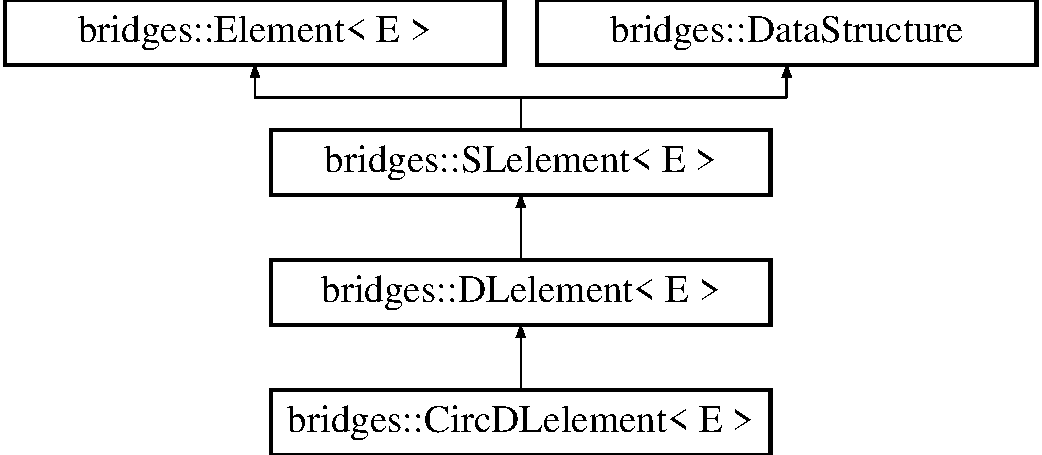
\includegraphics[height=4.000000cm]{classbridges_1_1_circ_d_lelement}
\end{center}
\end{figure}
\doxysubsection*{Public Member Functions}
\begin{DoxyCompactItemize}
\item 
\mbox{\hyperlink{classbridges_1_1_circ_d_lelement_a35279302f5fb5297eeb6efead475921e}{Circ\+D\+Lelement}} ()
\item 
\mbox{\hyperlink{classbridges_1_1_circ_d_lelement_a7dc1ad0eca7c06678064789303c522ed}{Circ\+D\+Lelement}} (E e, string label)
\item 
\mbox{\hyperlink{classbridges_1_1_circ_d_lelement_a9d0cf8a5b60e3fedc1ba1ad792570934}{Circ\+D\+Lelement}} (\mbox{\hyperlink{classbridges_1_1_circ_d_lelement}{Circ\+D\+Lelement}}$<$ E $>$ \mbox{\hyperlink{classbridges_1_1_s_lelement_ad7449d10a09ebc52653a7baed812aa43}{next}}, \mbox{\hyperlink{classbridges_1_1_circ_d_lelement}{Circ\+D\+Lelement}}$<$ E $>$ prev)
\item 
\mbox{\hyperlink{classbridges_1_1_circ_d_lelement_a2e729cd481f11c51bb5b686b8072ec8c}{Circ\+D\+Lelement}} (E e, \mbox{\hyperlink{classbridges_1_1_circ_d_lelement}{Circ\+D\+Lelement}}$<$ E $>$ \mbox{\hyperlink{classbridges_1_1_s_lelement_ad7449d10a09ebc52653a7baed812aa43}{next}}, \mbox{\hyperlink{classbridges_1_1_circ_d_lelement}{Circ\+D\+Lelement}}$<$ E $>$ prev)
\item 
virtual const string \mbox{\hyperlink{classbridges_1_1_circ_d_lelement_a0e199fe681755df694807261ce2460c2}{get\+D\+Stype}} () const override
\item 
const \mbox{\hyperlink{classbridges_1_1_circ_d_lelement}{Circ\+D\+Lelement}}$<$ E $>$ $\ast$ \mbox{\hyperlink{classbridges_1_1_circ_d_lelement_ac266d60bd2f7ce92cb38a12875a6a468}{get\+Next}} () const override
\item 
virtual \mbox{\hyperlink{classbridges_1_1_circ_d_lelement}{Circ\+D\+Lelement}}$<$ E $>$ $\ast$ \mbox{\hyperlink{classbridges_1_1_circ_d_lelement_a52996d42efc5680d1f8b406143abfee5}{get\+Next}} () override
\item 
void \mbox{\hyperlink{classbridges_1_1_circ_d_lelement_a0bdf28de82173f2099673d18f6f62810}{set\+Next}} (\mbox{\hyperlink{classbridges_1_1_circ_d_lelement}{Circ\+D\+Lelement}}$<$ E $>$ $\ast$\mbox{\hyperlink{classbridges_1_1_s_lelement_ad7449d10a09ebc52653a7baed812aa43}{next}})
\item 
const \mbox{\hyperlink{classbridges_1_1_circ_d_lelement}{Circ\+D\+Lelement}}$<$ E $>$ $\ast$ \mbox{\hyperlink{classbridges_1_1_circ_d_lelement_a8a1aa2f979094bccf2cca2ca31f0373d}{get\+Prev}} () const
\item 
void \mbox{\hyperlink{classbridges_1_1_circ_d_lelement_a5b2a0dad47208829bb2c17d8bc0ee74d}{set\+Prev}} (\mbox{\hyperlink{classbridges_1_1_circ_d_lelement}{Circ\+D\+Lelement}}$<$ E $>$ $\ast$prev)
\end{DoxyCompactItemize}
\doxysubsection*{Additional Inherited Members}


\doxysubsection{Detailed Description}
\subsubsection*{template$<$typename E$>$\newline
class bridges\+::\+Circ\+D\+Lelement$<$ E $>$}

This class can be used to instantiate Circular Doubly Linked List Elements. 

\begin{DoxyAuthor}{Author}
Kalpathi Subramanian 
\end{DoxyAuthor}
\begin{DoxyDate}{Date}
10/5/16
\end{DoxyDate}
Structurally they are the same as doubly linked elements except that each node constructed with the next and the previous pointers pointing to itself.

User\textquotesingle{}s implementation of the circularly linked list needs to ensure that the last node\textquotesingle{}s next pointer points to the first node and the first node\textquotesingle{}s previous pointer points to the last node, as the visualization generation is dependent on this.

Elements have labels (string) that are displayed on the visualization. Elements take an generic object E as a user defined parameter, which can any native type or object. Elements contain a visualizer object for setting visual attributes (color, shape, opacity, size), necessary for displaying them in a web browser 

\doxysubsection{Constructor \& Destructor Documentation}
\mbox{\Hypertarget{classbridges_1_1_circ_d_lelement_a35279302f5fb5297eeb6efead475921e}\label{classbridges_1_1_circ_d_lelement_a35279302f5fb5297eeb6efead475921e}} 
\index{bridges::CircDLelement$<$ E $>$@{bridges::CircDLelement$<$ E $>$}!CircDLelement@{CircDLelement}}
\index{CircDLelement@{CircDLelement}!bridges::CircDLelement$<$ E $>$@{bridges::CircDLelement$<$ E $>$}}
\doxysubsubsection{\texorpdfstring{CircDLelement()}{CircDLelement()}\hspace{0.1cm}{\footnotesize\ttfamily [1/4]}}
{\footnotesize\ttfamily template$<$typename E$>$ \\
\mbox{\hyperlink{classbridges_1_1_circ_d_lelement}{bridges\+::\+Circ\+D\+Lelement}}$<$ E $>$\+::\mbox{\hyperlink{classbridges_1_1_circ_d_lelement}{Circ\+D\+Lelement}} (\begin{DoxyParamCaption}{ }\end{DoxyParamCaption})\hspace{0.3cm}{\ttfamily [inline]}}

Constructs an empty \mbox{\hyperlink{classbridges_1_1_circ_d_lelement}{Circ\+D\+Lelement}} with next and prev pointers set to itself \mbox{\Hypertarget{classbridges_1_1_circ_d_lelement_a7dc1ad0eca7c06678064789303c522ed}\label{classbridges_1_1_circ_d_lelement_a7dc1ad0eca7c06678064789303c522ed}} 
\index{bridges::CircDLelement$<$ E $>$@{bridges::CircDLelement$<$ E $>$}!CircDLelement@{CircDLelement}}
\index{CircDLelement@{CircDLelement}!bridges::CircDLelement$<$ E $>$@{bridges::CircDLelement$<$ E $>$}}
\doxysubsubsection{\texorpdfstring{CircDLelement()}{CircDLelement()}\hspace{0.1cm}{\footnotesize\ttfamily [2/4]}}
{\footnotesize\ttfamily template$<$typename E$>$ \\
\mbox{\hyperlink{classbridges_1_1_circ_d_lelement}{bridges\+::\+Circ\+D\+Lelement}}$<$ E $>$\+::\mbox{\hyperlink{classbridges_1_1_circ_d_lelement}{Circ\+D\+Lelement}} (\begin{DoxyParamCaption}\item[{E}]{e,  }\item[{string}]{label }\end{DoxyParamCaption})\hspace{0.3cm}{\ttfamily [inline]}}

Constructs a \mbox{\hyperlink{classbridges_1_1_circ_d_lelement}{Circ\+D\+Lelement}} labeled \char`\"{}label\char`\"{}, holding an object \char`\"{}e\char`\"{}, with next and prev pointers set to itself 
\begin{DoxyParams}{Parameters}
{\em e} & the genereic object that this \mbox{\hyperlink{classbridges_1_1_circ_d_lelement}{Circ\+D\+Lelement}} is holding \\
\hline
{\em label} & the label for this \mbox{\hyperlink{classbridges_1_1_circ_d_lelement}{Circ\+D\+Lelement}} that shows up on the \mbox{\hyperlink{classbridges_1_1_bridges}{Bridges}} visualization \\
\hline
\end{DoxyParams}
\mbox{\Hypertarget{classbridges_1_1_circ_d_lelement_a9d0cf8a5b60e3fedc1ba1ad792570934}\label{classbridges_1_1_circ_d_lelement_a9d0cf8a5b60e3fedc1ba1ad792570934}} 
\index{bridges::CircDLelement$<$ E $>$@{bridges::CircDLelement$<$ E $>$}!CircDLelement@{CircDLelement}}
\index{CircDLelement@{CircDLelement}!bridges::CircDLelement$<$ E $>$@{bridges::CircDLelement$<$ E $>$}}
\doxysubsubsection{\texorpdfstring{CircDLelement()}{CircDLelement()}\hspace{0.1cm}{\footnotesize\ttfamily [3/4]}}
{\footnotesize\ttfamily template$<$typename E$>$ \\
\mbox{\hyperlink{classbridges_1_1_circ_d_lelement}{bridges\+::\+Circ\+D\+Lelement}}$<$ E $>$\+::\mbox{\hyperlink{classbridges_1_1_circ_d_lelement}{Circ\+D\+Lelement}} (\begin{DoxyParamCaption}\item[{\mbox{\hyperlink{classbridges_1_1_circ_d_lelement}{Circ\+D\+Lelement}}$<$ E $>$}]{next,  }\item[{\mbox{\hyperlink{classbridges_1_1_circ_d_lelement}{Circ\+D\+Lelement}}$<$ E $>$}]{prev }\end{DoxyParamCaption})\hspace{0.3cm}{\ttfamily [inline]}}

Constructs an empty \mbox{\hyperlink{classbridges_1_1_d_lelement}{D\+Lelement}} with the next pointer set to the \mbox{\hyperlink{classbridges_1_1_circ_d_lelement}{Circ\+D\+Lelement}} \char`\"{}next\char`\"{} and the prev pointer set to \mbox{\hyperlink{classbridges_1_1_circ_d_lelement}{Circ\+D\+Lelement}} \char`\"{}prev\char`\"{}.


\begin{DoxyParams}{Parameters}
{\em next} & the \mbox{\hyperlink{classbridges_1_1_d_lelement}{D\+Lelement}} that should be assigned to the next pointer \\
\hline
{\em prev} & the \mbox{\hyperlink{classbridges_1_1_d_lelement}{D\+Lelement}} that should be assigned to the prev pointer \\
\hline
\end{DoxyParams}
\mbox{\Hypertarget{classbridges_1_1_circ_d_lelement_a2e729cd481f11c51bb5b686b8072ec8c}\label{classbridges_1_1_circ_d_lelement_a2e729cd481f11c51bb5b686b8072ec8c}} 
\index{bridges::CircDLelement$<$ E $>$@{bridges::CircDLelement$<$ E $>$}!CircDLelement@{CircDLelement}}
\index{CircDLelement@{CircDLelement}!bridges::CircDLelement$<$ E $>$@{bridges::CircDLelement$<$ E $>$}}
\doxysubsubsection{\texorpdfstring{CircDLelement()}{CircDLelement()}\hspace{0.1cm}{\footnotesize\ttfamily [4/4]}}
{\footnotesize\ttfamily template$<$typename E$>$ \\
\mbox{\hyperlink{classbridges_1_1_circ_d_lelement}{bridges\+::\+Circ\+D\+Lelement}}$<$ E $>$\+::\mbox{\hyperlink{classbridges_1_1_circ_d_lelement}{Circ\+D\+Lelement}} (\begin{DoxyParamCaption}\item[{E}]{e,  }\item[{\mbox{\hyperlink{classbridges_1_1_circ_d_lelement}{Circ\+D\+Lelement}}$<$ E $>$}]{next,  }\item[{\mbox{\hyperlink{classbridges_1_1_circ_d_lelement}{Circ\+D\+Lelement}}$<$ E $>$}]{prev }\end{DoxyParamCaption})\hspace{0.3cm}{\ttfamily [inline]}}

Constructs a \mbox{\hyperlink{classbridges_1_1_d_lelement}{D\+Lelement}} holding an object \char`\"{}e\char`\"{}, with the next pointer set to the \mbox{\hyperlink{classbridges_1_1_d_lelement}{D\+Lelement}} \char`\"{}next\char`\"{} and the prev pointer set to \mbox{\hyperlink{classbridges_1_1_d_lelement}{D\+Lelement}} \char`\"{}prev\char`\"{}.


\begin{DoxyParams}{Parameters}
{\em e} & the genereic object that this \mbox{\hyperlink{classbridges_1_1_circ_d_lelement}{Circ\+D\+Lelement}} is holding \\
\hline
{\em next} & the \mbox{\hyperlink{classbridges_1_1_circ_d_lelement}{Circ\+D\+Lelement}} that should be assigned to the next pointer \\
\hline
{\em prev} & the \mbox{\hyperlink{classbridges_1_1_circ_d_lelement}{Circ\+D\+Lelement}} that should be assigned to the prev pointer \\
\hline
\end{DoxyParams}


\doxysubsection{Member Function Documentation}
\mbox{\Hypertarget{classbridges_1_1_circ_d_lelement_a0e199fe681755df694807261ce2460c2}\label{classbridges_1_1_circ_d_lelement_a0e199fe681755df694807261ce2460c2}} 
\index{bridges::CircDLelement$<$ E $>$@{bridges::CircDLelement$<$ E $>$}!getDStype@{getDStype}}
\index{getDStype@{getDStype}!bridges::CircDLelement$<$ E $>$@{bridges::CircDLelement$<$ E $>$}}
\doxysubsubsection{\texorpdfstring{getDStype()}{getDStype()}}
{\footnotesize\ttfamily template$<$typename E$>$ \\
virtual const string \mbox{\hyperlink{classbridges_1_1_circ_d_lelement}{bridges\+::\+Circ\+D\+Lelement}}$<$ E $>$\+::get\+D\+Stype (\begin{DoxyParamCaption}{ }\end{DoxyParamCaption}) const\hspace{0.3cm}{\ttfamily [inline]}, {\ttfamily [override]}, {\ttfamily [virtual]}}

This method gets the data structure type

\begin{DoxyReturn}{Returns}
The date structure type as a string 
\end{DoxyReturn}


Reimplemented from \mbox{\hyperlink{classbridges_1_1_d_lelement_a109be7aba8bd3d0450859938b5d3144c}{bridges\+::\+D\+Lelement$<$ E $>$}}.

\mbox{\Hypertarget{classbridges_1_1_circ_d_lelement_ac266d60bd2f7ce92cb38a12875a6a468}\label{classbridges_1_1_circ_d_lelement_ac266d60bd2f7ce92cb38a12875a6a468}} 
\index{bridges::CircDLelement$<$ E $>$@{bridges::CircDLelement$<$ E $>$}!getNext@{getNext}}
\index{getNext@{getNext}!bridges::CircDLelement$<$ E $>$@{bridges::CircDLelement$<$ E $>$}}
\doxysubsubsection{\texorpdfstring{getNext()}{getNext()}\hspace{0.1cm}{\footnotesize\ttfamily [1/2]}}
{\footnotesize\ttfamily template$<$typename E$>$ \\
const \mbox{\hyperlink{classbridges_1_1_circ_d_lelement}{Circ\+D\+Lelement}}$<$E$>$$\ast$ \mbox{\hyperlink{classbridges_1_1_circ_d_lelement}{bridges\+::\+Circ\+D\+Lelement}}$<$ E $>$\+::get\+Next (\begin{DoxyParamCaption}{ }\end{DoxyParamCaption}) const\hspace{0.3cm}{\ttfamily [inline]}, {\ttfamily [override]}, {\ttfamily [virtual]}}

This method returns the pointer to the next \mbox{\hyperlink{classbridges_1_1_d_lelement}{D\+Lelement}} \begin{DoxyReturn}{Returns}
the \mbox{\hyperlink{classbridges_1_1_d_lelement}{D\+Lelement}} assigned to the next pointer 
\end{DoxyReturn}


Reimplemented from \mbox{\hyperlink{classbridges_1_1_d_lelement_a648012849263b4b1cd2d504d5e5fd880}{bridges\+::\+D\+Lelement$<$ E $>$}}.

\mbox{\Hypertarget{classbridges_1_1_circ_d_lelement_a52996d42efc5680d1f8b406143abfee5}\label{classbridges_1_1_circ_d_lelement_a52996d42efc5680d1f8b406143abfee5}} 
\index{bridges::CircDLelement$<$ E $>$@{bridges::CircDLelement$<$ E $>$}!getNext@{getNext}}
\index{getNext@{getNext}!bridges::CircDLelement$<$ E $>$@{bridges::CircDLelement$<$ E $>$}}
\doxysubsubsection{\texorpdfstring{getNext()}{getNext()}\hspace{0.1cm}{\footnotesize\ttfamily [2/2]}}
{\footnotesize\ttfamily template$<$typename E$>$ \\
virtual \mbox{\hyperlink{classbridges_1_1_circ_d_lelement}{Circ\+D\+Lelement}}$<$E$>$$\ast$ \mbox{\hyperlink{classbridges_1_1_circ_d_lelement}{bridges\+::\+Circ\+D\+Lelement}}$<$ E $>$\+::get\+Next (\begin{DoxyParamCaption}{ }\end{DoxyParamCaption})\hspace{0.3cm}{\ttfamily [inline]}, {\ttfamily [override]}, {\ttfamily [virtual]}}

Retrieves the next \mbox{\hyperlink{classbridges_1_1_circ_s_lelement}{Circ\+S\+Lelement}} \begin{DoxyReturn}{Returns}
Circ\+S\+Lelement$<$\+E$>$ assigned to next 
\end{DoxyReturn}


Reimplemented from \mbox{\hyperlink{classbridges_1_1_d_lelement_a0c713707d8c7d0a97fe4194ed6592ede}{bridges\+::\+D\+Lelement$<$ E $>$}}.

\mbox{\Hypertarget{classbridges_1_1_circ_d_lelement_a8a1aa2f979094bccf2cca2ca31f0373d}\label{classbridges_1_1_circ_d_lelement_a8a1aa2f979094bccf2cca2ca31f0373d}} 
\index{bridges::CircDLelement$<$ E $>$@{bridges::CircDLelement$<$ E $>$}!getPrev@{getPrev}}
\index{getPrev@{getPrev}!bridges::CircDLelement$<$ E $>$@{bridges::CircDLelement$<$ E $>$}}
\doxysubsubsection{\texorpdfstring{getPrev()}{getPrev()}}
{\footnotesize\ttfamily template$<$typename E$>$ \\
const \mbox{\hyperlink{classbridges_1_1_circ_d_lelement}{Circ\+D\+Lelement}}$<$E$>$$\ast$ \mbox{\hyperlink{classbridges_1_1_circ_d_lelement}{bridges\+::\+Circ\+D\+Lelement}}$<$ E $>$\+::get\+Prev (\begin{DoxyParamCaption}{ }\end{DoxyParamCaption}) const\hspace{0.3cm}{\ttfamily [inline]}}

This method returns the pointer to the previous \mbox{\hyperlink{classbridges_1_1_d_lelement}{D\+Lelement}} \begin{DoxyReturn}{Returns}
the \mbox{\hyperlink{classbridges_1_1_d_lelement}{D\+Lelement}} assigned to the prev pointer 
\end{DoxyReturn}
\mbox{\Hypertarget{classbridges_1_1_circ_d_lelement_a0bdf28de82173f2099673d18f6f62810}\label{classbridges_1_1_circ_d_lelement_a0bdf28de82173f2099673d18f6f62810}} 
\index{bridges::CircDLelement$<$ E $>$@{bridges::CircDLelement$<$ E $>$}!setNext@{setNext}}
\index{setNext@{setNext}!bridges::CircDLelement$<$ E $>$@{bridges::CircDLelement$<$ E $>$}}
\doxysubsubsection{\texorpdfstring{setNext()}{setNext()}}
{\footnotesize\ttfamily template$<$typename E$>$ \\
void \mbox{\hyperlink{classbridges_1_1_circ_d_lelement}{bridges\+::\+Circ\+D\+Lelement}}$<$ E $>$\+::set\+Next (\begin{DoxyParamCaption}\item[{\mbox{\hyperlink{classbridges_1_1_circ_d_lelement}{Circ\+D\+Lelement}}$<$ E $>$ $\ast$}]{next }\end{DoxyParamCaption})\hspace{0.3cm}{\ttfamily [inline]}}

This method sets the pointer to the next \mbox{\hyperlink{classbridges_1_1_d_lelement}{D\+Lelement}}


\begin{DoxyParams}{Parameters}
{\em next} & the \mbox{\hyperlink{classbridges_1_1_d_lelement}{D\+Lelement}} that should be assigned to the next pointer \\
\hline
\end{DoxyParams}
\mbox{\Hypertarget{classbridges_1_1_circ_d_lelement_a5b2a0dad47208829bb2c17d8bc0ee74d}\label{classbridges_1_1_circ_d_lelement_a5b2a0dad47208829bb2c17d8bc0ee74d}} 
\index{bridges::CircDLelement$<$ E $>$@{bridges::CircDLelement$<$ E $>$}!setPrev@{setPrev}}
\index{setPrev@{setPrev}!bridges::CircDLelement$<$ E $>$@{bridges::CircDLelement$<$ E $>$}}
\doxysubsubsection{\texorpdfstring{setPrev()}{setPrev()}}
{\footnotesize\ttfamily template$<$typename E$>$ \\
void \mbox{\hyperlink{classbridges_1_1_circ_d_lelement}{bridges\+::\+Circ\+D\+Lelement}}$<$ E $>$\+::set\+Prev (\begin{DoxyParamCaption}\item[{\mbox{\hyperlink{classbridges_1_1_circ_d_lelement}{Circ\+D\+Lelement}}$<$ E $>$ $\ast$}]{prev }\end{DoxyParamCaption})\hspace{0.3cm}{\ttfamily [inline]}}

This method sets the pointer to the previous \mbox{\hyperlink{classbridges_1_1_d_lelement}{D\+Lelement}} 
\begin{DoxyParams}{Parameters}
{\em prev} & the \mbox{\hyperlink{classbridges_1_1_d_lelement}{D\+Lelement}} that should be assigned to the prev pointer \\
\hline
\end{DoxyParams}


The documentation for this class was generated from the following file\+:\begin{DoxyCompactItemize}
\item 
/\+Users/kalpathi/gr/bridges/client/c++/src/\mbox{\hyperlink{_circ_d_lelement_8h}{Circ\+D\+Lelement.\+h}}\end{DoxyCompactItemize}

\hypertarget{classbridges_1_1_circ_s_lelement}{}\doxysection{bridges\+::Circ\+S\+Lelement$<$ E $>$ Class Template Reference}
\label{classbridges_1_1_circ_s_lelement}\index{bridges::CircSLelement$<$ E $>$@{bridges::CircSLelement$<$ E $>$}}


This class can be used to instantiate Singly Linked Circular List Elements.  




{\ttfamily \#include $<$Circ\+S\+Lelement.\+h$>$}

Inheritance diagram for bridges\+::Circ\+S\+Lelement$<$ E $>$\+:\begin{figure}[H]
\begin{center}
\leavevmode
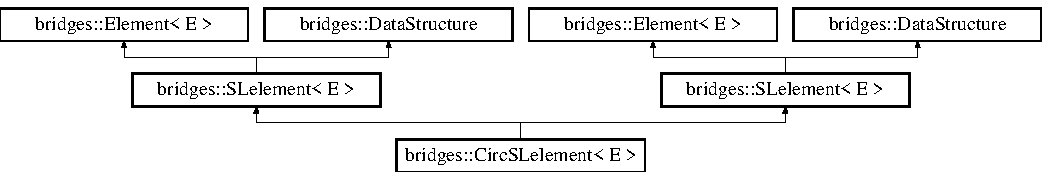
\includegraphics[height=3.000000cm]{classbridges_1_1_circ_s_lelement}
\end{center}
\end{figure}
\doxysubsection*{Public Member Functions}
\begin{DoxyCompactItemize}
\item 
\mbox{\hyperlink{classbridges_1_1_circ_s_lelement_a86183d3487b906550d8f32bda3a68f98}{Circ\+S\+Lelement}} ()
\item 
\mbox{\hyperlink{classbridges_1_1_circ_s_lelement_a765032df6cfaa7cf7589c9e0df29bae4}{Circ\+S\+Lelement}} (E val=E(), string label=string())
\item 
\mbox{\hyperlink{classbridges_1_1_circ_s_lelement_a0dd7605959b4b52de041e9bcbe5abce7}{Circ\+S\+Lelement}} (E e=E(), \mbox{\hyperlink{classbridges_1_1_circ_s_lelement}{Circ\+S\+Lelement}} $\ast$\mbox{\hyperlink{classbridges_1_1_s_lelement_ad7449d10a09ebc52653a7baed812aa43}{next}}=nullptr)
\item 
\mbox{\hyperlink{classbridges_1_1_circ_s_lelement_a1fda146fc0da1d8c7d6440cbbbb2ce42}{Circ\+S\+Lelement}} (\mbox{\hyperlink{classbridges_1_1_circ_s_lelement}{Circ\+S\+Lelement}} $\ast$\mbox{\hyperlink{classbridges_1_1_s_lelement_ad7449d10a09ebc52653a7baed812aa43}{next}})
\item 
virtual const string \mbox{\hyperlink{classbridges_1_1_circ_s_lelement_a4b27c205af46162371e3ffe05cbbe3d5}{get\+D\+Stype}} () const override
\item 
virtual \mbox{\hyperlink{classbridges_1_1_circ_s_lelement}{Circ\+S\+Lelement}}$<$ E $>$ $\ast$ \mbox{\hyperlink{classbridges_1_1_circ_s_lelement_aab863627c125c6f1075af7e7b7f340cf}{get\+Next}} () override
\item 
void \mbox{\hyperlink{classbridges_1_1_circ_s_lelement_a7b2512dd1cc559f0a89d9ab4aafed172}{set\+Next}} (\mbox{\hyperlink{classbridges_1_1_circ_s_lelement}{Circ\+S\+Lelement}}$<$ E $>$ $\ast$\mbox{\hyperlink{classbridges_1_1_s_lelement_ad7449d10a09ebc52653a7baed812aa43}{next}})
\end{DoxyCompactItemize}
\doxysubsection*{Additional Inherited Members}


\doxysubsection{Detailed Description}
\subsubsection*{template$<$typename E$>$\newline
class bridges\+::\+Circ\+S\+Lelement$<$ E $>$}

This class can be used to instantiate Singly Linked Circular List Elements. 

This class can be used to instantiate Circular (Singly) Linked List Elements, derived from Singly Linked \mbox{\hyperlink{classbridges_1_1_element}{Element}}. The main difference from the \mbox{\hyperlink{classbridges_1_1_s_lelement}{S\+Lelement}} is that they create circularly linked elements and their traversals are slightly different.

Elements have labels (string) that are displayed on the visualization Elements take an generic object as a user defined parameter, any native type or object.

\mbox{\hyperlink{classbridges_1_1_element}{Element}} contains a visualizer object for setting visual attributes (color, shape, opacity, size), necessary for displaying them in a web browser

\begin{DoxyAuthor}{Author}
Kalpathi Subramanian 
\end{DoxyAuthor}
\begin{DoxyDate}{Date}
10/5/2016
\end{DoxyDate}

\begin{DoxyParams}{Parameters}
{\em $<$\+E$>$} & \\
\hline
\end{DoxyParams}


\doxysubsection{Constructor \& Destructor Documentation}
\mbox{\Hypertarget{classbridges_1_1_circ_s_lelement_a86183d3487b906550d8f32bda3a68f98}\label{classbridges_1_1_circ_s_lelement_a86183d3487b906550d8f32bda3a68f98}} 
\index{bridges::CircSLelement$<$ E $>$@{bridges::CircSLelement$<$ E $>$}!CircSLelement@{CircSLelement}}
\index{CircSLelement@{CircSLelement}!bridges::CircSLelement$<$ E $>$@{bridges::CircSLelement$<$ E $>$}}
\doxysubsubsection{\texorpdfstring{CircSLelement()}{CircSLelement()}\hspace{0.1cm}{\footnotesize\ttfamily [1/4]}}
{\footnotesize\ttfamily template$<$typename E$>$ \\
\mbox{\hyperlink{classbridges_1_1_circ_s_lelement}{bridges\+::\+Circ\+S\+Lelement}}$<$ E $>$\+::\mbox{\hyperlink{classbridges_1_1_circ_s_lelement}{Circ\+S\+Lelement}} (\begin{DoxyParamCaption}{ }\end{DoxyParamCaption})\hspace{0.3cm}{\ttfamily [inline]}}

This constructor creates an \mbox{\hyperlink{classbridges_1_1_circ_s_lelement}{Circ\+S\+Lelement}} object and sets its next pointer to itself \mbox{\Hypertarget{classbridges_1_1_circ_s_lelement_a765032df6cfaa7cf7589c9e0df29bae4}\label{classbridges_1_1_circ_s_lelement_a765032df6cfaa7cf7589c9e0df29bae4}} 
\index{bridges::CircSLelement$<$ E $>$@{bridges::CircSLelement$<$ E $>$}!CircSLelement@{CircSLelement}}
\index{CircSLelement@{CircSLelement}!bridges::CircSLelement$<$ E $>$@{bridges::CircSLelement$<$ E $>$}}
\doxysubsubsection{\texorpdfstring{CircSLelement()}{CircSLelement()}\hspace{0.1cm}{\footnotesize\ttfamily [2/4]}}
{\footnotesize\ttfamily template$<$typename E$>$ \\
\mbox{\hyperlink{classbridges_1_1_circ_s_lelement}{bridges\+::\+Circ\+S\+Lelement}}$<$ E $>$\+::\mbox{\hyperlink{classbridges_1_1_circ_s_lelement}{Circ\+S\+Lelement}} (\begin{DoxyParamCaption}\item[{E}]{val = {\ttfamily E()},  }\item[{string}]{label = {\ttfamily string()} }\end{DoxyParamCaption})\hspace{0.3cm}{\ttfamily [inline]}}

This constructor creates an \mbox{\hyperlink{classbridges_1_1_circ_s_lelement}{Circ\+S\+Lelement}} object of value \char`\"{}e\char`\"{} and label \char`\"{}label\char`\"{} and sets the next pointer to null


\begin{DoxyParams}{Parameters}
{\em label} & the label of \mbox{\hyperlink{classbridges_1_1_circ_s_lelement}{Circ\+S\+Lelement}} that shows up on the \mbox{\hyperlink{classbridges_1_1_bridges}{Bridges}} visualization \\
\hline
{\em e} & the generic object that this \mbox{\hyperlink{classbridges_1_1_circ_s_lelement}{Circ\+S\+Lelement}} will hold \\
\hline
\end{DoxyParams}
\mbox{\Hypertarget{classbridges_1_1_circ_s_lelement_a0dd7605959b4b52de041e9bcbe5abce7}\label{classbridges_1_1_circ_s_lelement_a0dd7605959b4b52de041e9bcbe5abce7}} 
\index{bridges::CircSLelement$<$ E $>$@{bridges::CircSLelement$<$ E $>$}!CircSLelement@{CircSLelement}}
\index{CircSLelement@{CircSLelement}!bridges::CircSLelement$<$ E $>$@{bridges::CircSLelement$<$ E $>$}}
\doxysubsubsection{\texorpdfstring{CircSLelement()}{CircSLelement()}\hspace{0.1cm}{\footnotesize\ttfamily [3/4]}}
{\footnotesize\ttfamily template$<$typename E$>$ \\
\mbox{\hyperlink{classbridges_1_1_circ_s_lelement}{bridges\+::\+Circ\+S\+Lelement}}$<$ E $>$\+::\mbox{\hyperlink{classbridges_1_1_circ_s_lelement}{Circ\+S\+Lelement}} (\begin{DoxyParamCaption}\item[{E}]{e = {\ttfamily E()},  }\item[{\mbox{\hyperlink{classbridges_1_1_circ_s_lelement}{Circ\+S\+Lelement}}$<$ E $>$ $\ast$}]{next = {\ttfamily nullptr} }\end{DoxyParamCaption})\hspace{0.3cm}{\ttfamily [inline]}}

Creates a new element with value \char`\"{}e\char`\"{} and sets the next pointer to the \mbox{\hyperlink{classbridges_1_1_circ_s_lelement}{Circ\+S\+Lelement}} referenced by the \char`\"{}next\char`\"{} argument


\begin{DoxyParams}{Parameters}
{\em e} & the generic object that this \mbox{\hyperlink{classbridges_1_1_circ_s_lelement}{Circ\+S\+Lelement}} will hold \\
\hline
{\em next} & the \mbox{\hyperlink{classbridges_1_1_circ_s_lelement}{Circ\+S\+Lelement}} that should be assigned to the next pointer \\
\hline
\end{DoxyParams}
\mbox{\Hypertarget{classbridges_1_1_circ_s_lelement_a1fda146fc0da1d8c7d6440cbbbb2ce42}\label{classbridges_1_1_circ_s_lelement_a1fda146fc0da1d8c7d6440cbbbb2ce42}} 
\index{bridges::CircSLelement$<$ E $>$@{bridges::CircSLelement$<$ E $>$}!CircSLelement@{CircSLelement}}
\index{CircSLelement@{CircSLelement}!bridges::CircSLelement$<$ E $>$@{bridges::CircSLelement$<$ E $>$}}
\doxysubsubsection{\texorpdfstring{CircSLelement()}{CircSLelement()}\hspace{0.1cm}{\footnotesize\ttfamily [4/4]}}
{\footnotesize\ttfamily template$<$typename E$>$ \\
\mbox{\hyperlink{classbridges_1_1_circ_s_lelement}{bridges\+::\+Circ\+S\+Lelement}}$<$ E $>$\+::\mbox{\hyperlink{classbridges_1_1_circ_s_lelement}{Circ\+S\+Lelement}} (\begin{DoxyParamCaption}\item[{\mbox{\hyperlink{classbridges_1_1_circ_s_lelement}{Circ\+S\+Lelement}}$<$ E $>$ $\ast$}]{next }\end{DoxyParamCaption})\hspace{0.3cm}{\ttfamily [inline]}}

Creates a new element and sets the next pointer to the \mbox{\hyperlink{classbridges_1_1_circ_s_lelement}{Circ\+S\+Lelement}} \char`\"{}next\char`\"{} 
\begin{DoxyParams}{Parameters}
{\em next} & the \mbox{\hyperlink{classbridges_1_1_circ_s_lelement}{Circ\+S\+Lelement}} that should be assigned to the next pointer \\
\hline
\end{DoxyParams}


\doxysubsection{Member Function Documentation}
\mbox{\Hypertarget{classbridges_1_1_circ_s_lelement_a4b27c205af46162371e3ffe05cbbe3d5}\label{classbridges_1_1_circ_s_lelement_a4b27c205af46162371e3ffe05cbbe3d5}} 
\index{bridges::CircSLelement$<$ E $>$@{bridges::CircSLelement$<$ E $>$}!getDStype@{getDStype}}
\index{getDStype@{getDStype}!bridges::CircSLelement$<$ E $>$@{bridges::CircSLelement$<$ E $>$}}
\doxysubsubsection{\texorpdfstring{getDStype()}{getDStype()}}
{\footnotesize\ttfamily template$<$typename E$>$ \\
virtual const string \mbox{\hyperlink{classbridges_1_1_circ_s_lelement}{bridges\+::\+Circ\+S\+Lelement}}$<$ E $>$\+::get\+D\+Stype (\begin{DoxyParamCaption}{ }\end{DoxyParamCaption}) const\hspace{0.3cm}{\ttfamily [inline]}, {\ttfamily [override]}, {\ttfamily [virtual]}}

This method gets the data structure type

\begin{DoxyReturn}{Returns}
The date structure type as a string 
\end{DoxyReturn}


Reimplemented from \mbox{\hyperlink{classbridges_1_1_s_lelement_a136330b3481a47b3edb429f323274655}{bridges\+::\+S\+Lelement$<$ E $>$}}.

\mbox{\Hypertarget{classbridges_1_1_circ_s_lelement_aab863627c125c6f1075af7e7b7f340cf}\label{classbridges_1_1_circ_s_lelement_aab863627c125c6f1075af7e7b7f340cf}} 
\index{bridges::CircSLelement$<$ E $>$@{bridges::CircSLelement$<$ E $>$}!getNext@{getNext}}
\index{getNext@{getNext}!bridges::CircSLelement$<$ E $>$@{bridges::CircSLelement$<$ E $>$}}
\doxysubsubsection{\texorpdfstring{getNext()}{getNext()}}
{\footnotesize\ttfamily template$<$typename E$>$ \\
virtual \mbox{\hyperlink{classbridges_1_1_circ_s_lelement}{Circ\+S\+Lelement}}$<$E$>$$\ast$ \mbox{\hyperlink{classbridges_1_1_circ_s_lelement}{bridges\+::\+Circ\+S\+Lelement}}$<$ E $>$\+::get\+Next (\begin{DoxyParamCaption}{ }\end{DoxyParamCaption})\hspace{0.3cm}{\ttfamily [inline]}, {\ttfamily [override]}, {\ttfamily [virtual]}}

Retrieves the next \mbox{\hyperlink{classbridges_1_1_circ_s_lelement}{Circ\+S\+Lelement}} \begin{DoxyReturn}{Returns}
Circ\+S\+Lelement$<$\+E$>$ assigned to next 
\end{DoxyReturn}


Reimplemented from \mbox{\hyperlink{classbridges_1_1_s_lelement_a5bd74108a9aa49339378bf62cdbb19ca}{bridges\+::\+S\+Lelement$<$ E $>$}}.

\mbox{\Hypertarget{classbridges_1_1_circ_s_lelement_a7b2512dd1cc559f0a89d9ab4aafed172}\label{classbridges_1_1_circ_s_lelement_a7b2512dd1cc559f0a89d9ab4aafed172}} 
\index{bridges::CircSLelement$<$ E $>$@{bridges::CircSLelement$<$ E $>$}!setNext@{setNext}}
\index{setNext@{setNext}!bridges::CircSLelement$<$ E $>$@{bridges::CircSLelement$<$ E $>$}}
\doxysubsubsection{\texorpdfstring{setNext()}{setNext()}}
{\footnotesize\ttfamily template$<$typename E$>$ \\
void \mbox{\hyperlink{classbridges_1_1_circ_s_lelement}{bridges\+::\+Circ\+S\+Lelement}}$<$ E $>$\+::set\+Next (\begin{DoxyParamCaption}\item[{\mbox{\hyperlink{classbridges_1_1_circ_s_lelement}{Circ\+S\+Lelement}}$<$ E $>$ $\ast$}]{next }\end{DoxyParamCaption})\hspace{0.3cm}{\ttfamily [inline]}}

Sets the pointer to the next \mbox{\hyperlink{classbridges_1_1_circ_s_lelement}{Circ\+S\+Lelement}} 
\begin{DoxyParams}{Parameters}
{\em next} & Circ\+S\+Lelement$<$\+E$>$ that should be assigned to the next pointer \\
\hline
\end{DoxyParams}


The documentation for this class was generated from the following file\+:\begin{DoxyCompactItemize}
\item 
/\+Users/kalpathi/gr/bridges/client/c++/src/\mbox{\hyperlink{_circ_s_lelement_8h}{Circ\+S\+Lelement.\+h}}\end{DoxyCompactItemize}

\hypertarget{classbridges_1_1_color}{}\section{bridges\+:\+:Color Class Reference}
\label{classbridges_1_1_color}\index{bridges\+::\+Color@{bridges\+::\+Color}}


This class represents \mbox{\hyperlink{classbridges_1_1_color}{Color}}, and supports rgba, hexadecimal and named color values.  




{\ttfamily \#include $<$Color.\+h$>$}

\subsection*{Public Member Functions}
\begin{DoxyCompactItemize}
\item 
\mbox{\hyperlink{classbridges_1_1_color_ab89df8fea283d33585380ea91d78bbee}{Color}} ()
\item 
\mbox{\hyperlink{classbridges_1_1_color_aa861c0dc7729008cc4f886f235198181}{Color}} (const int \&r, const int \&g, const int \&b, const int \&a=255)
\item 
\mbox{\hyperlink{classbridges_1_1_color_a813c6cb59aad0883bcc12305fa6049cc}{Color}} (const string \&name)
\item 
bool \mbox{\hyperlink{classbridges_1_1_color_a9b33b4ee063496691f8816504cc8b007}{operator==}} (const \mbox{\hyperlink{classbridges_1_1_color}{Color}} \&that) const
\item 
bool \mbox{\hyperlink{classbridges_1_1_color_abe4ff1e5d4c6a33b2e9715be57ae0dce}{operator!=}} (const \mbox{\hyperlink{classbridges_1_1_color}{Color}} \&that) const
\item 
bool \mbox{\hyperlink{classbridges_1_1_color_ae55f3077cb3bd93386dc11eaeecf823c}{is\+Opaque}} () const
\item 
bool \mbox{\hyperlink{classbridges_1_1_color_a56b0d17239aafa0cea7f43e5358cf4c0}{is\+Transparent}} () const
\item 
int \mbox{\hyperlink{classbridges_1_1_color_a4c81e33854a6fdba9a3030e97ec8609e}{get\+Red}} () const
\item 
int \mbox{\hyperlink{classbridges_1_1_color_a93f8e016e1f1e6c177924ad8712e3e48}{get\+Green}} () const
\item 
int \mbox{\hyperlink{classbridges_1_1_color_aa7a70279f41f2cceb640162c43a2a382}{get\+Blue}} () const
\item 
int \mbox{\hyperlink{classbridges_1_1_color_a61523716f5597013d57bc98eae1fe96a}{get\+Alpha}} () const
\item 
string \mbox{\hyperlink{classbridges_1_1_color_a051fa9e828ce7025093c65c46358a8cf}{get\+Hex\+Value}} () const
\item 
void \mbox{\hyperlink{classbridges_1_1_color_a6d7521acce040aca88645f6ad1bf5f44}{set\+Red}} (int r)
\item 
void \mbox{\hyperlink{classbridges_1_1_color_a7689ebb07ae20ad846827e4f42546ba8}{set\+Green}} (int g)
\item 
void \mbox{\hyperlink{classbridges_1_1_color_a3b0e703dd68d7e695664264908e0f709}{set\+Blue}} (int b)
\item 
void \mbox{\hyperlink{classbridges_1_1_color_ab139e842be237a8963d46c6a3edb488d}{set\+Alpha}} (int a)
\item 
void \mbox{\hyperlink{classbridges_1_1_color_a3d6c66d33bd8a702a4436925c9cbd1fd}{set\+Value}} (int r, int g, int b, int a=255)
\item 
void \mbox{\hyperlink{classbridges_1_1_color_aa6e1db9aa47275ef829ac0fa96d72190}{set\+Value}} (string name)
\end{DoxyCompactItemize}


\subsection{Detailed Description}
This class represents \mbox{\hyperlink{classbridges_1_1_color}{Color}}, and supports rgba, hexadecimal and named color values. 

This class contains functions for the manipulation of a \mbox{\hyperlink{classbridges_1_1_color}{Color}} representation.

Supported rgba colors are integer representations of each color channel, in the range of \mbox{[}0,255\mbox{]}. rgb input is also supported, and given a default alpha value of 255(opaque)

Supported Hexadecimal colors are in the form \#\+R\+R\+G\+G\+B\+B\+AA, \#\+R\+R\+G\+G\+BB, \#\+R\+G\+BA, or \#\+R\+GB. With R,G,B and A, representing the Red, Green, Blue, and Alpha color channels respectivly, in hexadecimal digits(0-\/9a-\/f, base 16) prefixed by \textquotesingle{}\#\textquotesingle{}. \#\+R\+G\+BA and \#\+R\+GB are shorthand versions of \#\+R\+R\+G\+G\+B\+B\+AA and \#\+R\+R\+G\+G\+BB, where each channel pair is the same. If no alpha channel is provided, a default of \textquotesingle{}ff\textquotesingle{}(opaque) will be used

Supported named colors are\+: \char`\"{}red\char`\"{}, \char`\"{}yellow\char`\"{}, \char`\"{}blue\char`\"{}, \char`\"{}orange\char`\"{}, \char`\"{}green\char`\"{}, \char`\"{}purple\char`\"{}, \char`\"{}brown\char`\"{}, \char`\"{}black\char`\"{}, \char`\"{}grey\char`\"{}, and \char`\"{}white\char`\"{} All named colors have are fully opaque by default.

Default \mbox{\hyperlink{classbridges_1_1_color}{Color}} is opaque white

\begin{DoxyDate}{Date}
12/5/15, Dakota Carmer 
\end{DoxyDate}


\subsection{Constructor \& Destructor Documentation}
\mbox{\Hypertarget{classbridges_1_1_color_ab89df8fea283d33585380ea91d78bbee}\label{classbridges_1_1_color_ab89df8fea283d33585380ea91d78bbee}} 
\index{bridges\+::\+Color@{bridges\+::\+Color}!Color@{Color}}
\index{Color@{Color}!bridges\+::\+Color@{bridges\+::\+Color}}
\subsubsection{\texorpdfstring{Color()}{Color()}\hspace{0.1cm}{\footnotesize\ttfamily [1/3]}}
{\footnotesize\ttfamily bridges\+::\+Color\+::\+Color (\begin{DoxyParamCaption}{ }\end{DoxyParamCaption})\hspace{0.3cm}{\ttfamily [inline]}}

Default constructor Defaults to black \mbox{\Hypertarget{classbridges_1_1_color_aa861c0dc7729008cc4f886f235198181}\label{classbridges_1_1_color_aa861c0dc7729008cc4f886f235198181}} 
\index{bridges\+::\+Color@{bridges\+::\+Color}!Color@{Color}}
\index{Color@{Color}!bridges\+::\+Color@{bridges\+::\+Color}}
\subsubsection{\texorpdfstring{Color()}{Color()}\hspace{0.1cm}{\footnotesize\ttfamily [2/3]}}
{\footnotesize\ttfamily bridges\+::\+Color\+::\+Color (\begin{DoxyParamCaption}\item[{const int \&}]{r,  }\item[{const int \&}]{g,  }\item[{const int \&}]{b,  }\item[{const int \&}]{a = {\ttfamily 255} }\end{DoxyParamCaption})\hspace{0.3cm}{\ttfamily [inline]}}

Constructs a color with the specified rgba color channel values \mbox{[}0,255\mbox{]}. If no alpha channel is provided, the default of 255(opaque) is used.


\begin{DoxyParams}{Parameters}
{\em r} & The red channel \\
\hline
{\em g} & The green channel \\
\hline
{\em b} & The blue channel \\
\hline
{\em a} & The alpha channel(default 255) \\
\hline
\end{DoxyParams}
\mbox{\Hypertarget{classbridges_1_1_color_a813c6cb59aad0883bcc12305fa6049cc}\label{classbridges_1_1_color_a813c6cb59aad0883bcc12305fa6049cc}} 
\index{bridges\+::\+Color@{bridges\+::\+Color}!Color@{Color}}
\index{Color@{Color}!bridges\+::\+Color@{bridges\+::\+Color}}
\subsubsection{\texorpdfstring{Color()}{Color()}\hspace{0.1cm}{\footnotesize\ttfamily [3/3]}}
{\footnotesize\ttfamily bridges\+::\+Color\+::\+Color (\begin{DoxyParamCaption}\item[{const string \&}]{name }\end{DoxyParamCaption})\hspace{0.3cm}{\ttfamily [inline]}}

Constructs a color from a named color or a \#hexadecimal \mbox{[}0-\/F\mbox{]}(base 16) of the form \#\+R\+R\+G\+G\+B\+B\+AA, \#\+R\+R\+G\+G\+B\+B\+AA, \#\+R\+G\+BA, or \#\+R\+GB. Named colors and \#hexadecimals missing an alpha channel are made opaque.


\begin{DoxyParams}{Parameters}
{\em name} & The named color or \#hexadecimal value \\
\hline
\end{DoxyParams}


\subsection{Member Function Documentation}
\mbox{\Hypertarget{classbridges_1_1_color_a61523716f5597013d57bc98eae1fe96a}\label{classbridges_1_1_color_a61523716f5597013d57bc98eae1fe96a}} 
\index{bridges\+::\+Color@{bridges\+::\+Color}!get\+Alpha@{get\+Alpha}}
\index{get\+Alpha@{get\+Alpha}!bridges\+::\+Color@{bridges\+::\+Color}}
\subsubsection{\texorpdfstring{get\+Alpha()}{getAlpha()}}
{\footnotesize\ttfamily int bridges\+::\+Color\+::get\+Alpha (\begin{DoxyParamCaption}{ }\end{DoxyParamCaption}) const\hspace{0.3cm}{\ttfamily [inline]}}

\begin{DoxyReturn}{Returns}
rgba value of the alpha channel \mbox{[}0,255\mbox{]} 
\end{DoxyReturn}
\mbox{\Hypertarget{classbridges_1_1_color_aa7a70279f41f2cceb640162c43a2a382}\label{classbridges_1_1_color_aa7a70279f41f2cceb640162c43a2a382}} 
\index{bridges\+::\+Color@{bridges\+::\+Color}!get\+Blue@{get\+Blue}}
\index{get\+Blue@{get\+Blue}!bridges\+::\+Color@{bridges\+::\+Color}}
\subsubsection{\texorpdfstring{get\+Blue()}{getBlue()}}
{\footnotesize\ttfamily int bridges\+::\+Color\+::get\+Blue (\begin{DoxyParamCaption}{ }\end{DoxyParamCaption}) const\hspace{0.3cm}{\ttfamily [inline]}}

\begin{DoxyReturn}{Returns}
rgba value of the blue channel \mbox{[}0,255\mbox{]} 
\end{DoxyReturn}
\mbox{\Hypertarget{classbridges_1_1_color_a93f8e016e1f1e6c177924ad8712e3e48}\label{classbridges_1_1_color_a93f8e016e1f1e6c177924ad8712e3e48}} 
\index{bridges\+::\+Color@{bridges\+::\+Color}!get\+Green@{get\+Green}}
\index{get\+Green@{get\+Green}!bridges\+::\+Color@{bridges\+::\+Color}}
\subsubsection{\texorpdfstring{get\+Green()}{getGreen()}}
{\footnotesize\ttfamily int bridges\+::\+Color\+::get\+Green (\begin{DoxyParamCaption}{ }\end{DoxyParamCaption}) const\hspace{0.3cm}{\ttfamily [inline]}}

\begin{DoxyReturn}{Returns}
rgba value of the green channel \mbox{[}0,255\mbox{]} 
\end{DoxyReturn}
\mbox{\Hypertarget{classbridges_1_1_color_a051fa9e828ce7025093c65c46358a8cf}\label{classbridges_1_1_color_a051fa9e828ce7025093c65c46358a8cf}} 
\index{bridges\+::\+Color@{bridges\+::\+Color}!get\+Hex\+Value@{get\+Hex\+Value}}
\index{get\+Hex\+Value@{get\+Hex\+Value}!bridges\+::\+Color@{bridges\+::\+Color}}
\subsubsection{\texorpdfstring{get\+Hex\+Value()}{getHexValue()}}
{\footnotesize\ttfamily string bridges\+::\+Color\+::get\+Hex\+Value (\begin{DoxyParamCaption}{ }\end{DoxyParamCaption}) const\hspace{0.3cm}{\ttfamily [inline]}}

\begin{DoxyReturn}{Returns}
The \#hexadecimal representation (\#\+R\+R\+G\+G\+B\+B\+AA) of this color 
\end{DoxyReturn}
\mbox{\Hypertarget{classbridges_1_1_color_a4c81e33854a6fdba9a3030e97ec8609e}\label{classbridges_1_1_color_a4c81e33854a6fdba9a3030e97ec8609e}} 
\index{bridges\+::\+Color@{bridges\+::\+Color}!get\+Red@{get\+Red}}
\index{get\+Red@{get\+Red}!bridges\+::\+Color@{bridges\+::\+Color}}
\subsubsection{\texorpdfstring{get\+Red()}{getRed()}}
{\footnotesize\ttfamily int bridges\+::\+Color\+::get\+Red (\begin{DoxyParamCaption}{ }\end{DoxyParamCaption}) const\hspace{0.3cm}{\ttfamily [inline]}}

\begin{DoxyReturn}{Returns}
rgba value of the red channel \mbox{[}0,255\mbox{]} 
\end{DoxyReturn}
\mbox{\Hypertarget{classbridges_1_1_color_ae55f3077cb3bd93386dc11eaeecf823c}\label{classbridges_1_1_color_ae55f3077cb3bd93386dc11eaeecf823c}} 
\index{bridges\+::\+Color@{bridges\+::\+Color}!is\+Opaque@{is\+Opaque}}
\index{is\+Opaque@{is\+Opaque}!bridges\+::\+Color@{bridges\+::\+Color}}
\subsubsection{\texorpdfstring{is\+Opaque()}{isOpaque()}}
{\footnotesize\ttfamily bool bridges\+::\+Color\+::is\+Opaque (\begin{DoxyParamCaption}{ }\end{DoxyParamCaption}) const\hspace{0.3cm}{\ttfamily [inline]}}

\begin{DoxyReturn}{Returns}
True if fully opaque, false if not 
\end{DoxyReturn}
\mbox{\Hypertarget{classbridges_1_1_color_a56b0d17239aafa0cea7f43e5358cf4c0}\label{classbridges_1_1_color_a56b0d17239aafa0cea7f43e5358cf4c0}} 
\index{bridges\+::\+Color@{bridges\+::\+Color}!is\+Transparent@{is\+Transparent}}
\index{is\+Transparent@{is\+Transparent}!bridges\+::\+Color@{bridges\+::\+Color}}
\subsubsection{\texorpdfstring{is\+Transparent()}{isTransparent()}}
{\footnotesize\ttfamily bool bridges\+::\+Color\+::is\+Transparent (\begin{DoxyParamCaption}{ }\end{DoxyParamCaption}) const\hspace{0.3cm}{\ttfamily [inline]}}

\begin{DoxyReturn}{Returns}
True if fully transparent, false if not 
\end{DoxyReturn}
\mbox{\Hypertarget{classbridges_1_1_color_abe4ff1e5d4c6a33b2e9715be57ae0dce}\label{classbridges_1_1_color_abe4ff1e5d4c6a33b2e9715be57ae0dce}} 
\index{bridges\+::\+Color@{bridges\+::\+Color}!operator"!=@{operator"!=}}
\index{operator"!=@{operator"!=}!bridges\+::\+Color@{bridges\+::\+Color}}
\subsubsection{\texorpdfstring{operator"!=()}{operator!=()}}
{\footnotesize\ttfamily bool bridges\+::\+Color\+::operator!= (\begin{DoxyParamCaption}\item[{const \mbox{\hyperlink{classbridges_1_1_color}{Color}} \&}]{that }\end{DoxyParamCaption}) const\hspace{0.3cm}{\ttfamily [inline]}}

Inequality Comparison Operator \begin{DoxyReturn}{Returns}
False if both Colors represent the same \mbox{\hyperlink{classbridges_1_1_color}{Color}}, true if not 
\end{DoxyReturn}
\mbox{\Hypertarget{classbridges_1_1_color_a9b33b4ee063496691f8816504cc8b007}\label{classbridges_1_1_color_a9b33b4ee063496691f8816504cc8b007}} 
\index{bridges\+::\+Color@{bridges\+::\+Color}!operator==@{operator==}}
\index{operator==@{operator==}!bridges\+::\+Color@{bridges\+::\+Color}}
\subsubsection{\texorpdfstring{operator==()}{operator==()}}
{\footnotesize\ttfamily bool bridges\+::\+Color\+::operator== (\begin{DoxyParamCaption}\item[{const \mbox{\hyperlink{classbridges_1_1_color}{Color}} \&}]{that }\end{DoxyParamCaption}) const\hspace{0.3cm}{\ttfamily [inline]}}

Equality Comparison Operator \begin{DoxyReturn}{Returns}
True if both Colors represent the same \mbox{\hyperlink{classbridges_1_1_color}{Color}}, false if not 
\end{DoxyReturn}
\mbox{\Hypertarget{classbridges_1_1_color_ab139e842be237a8963d46c6a3edb488d}\label{classbridges_1_1_color_ab139e842be237a8963d46c6a3edb488d}} 
\index{bridges\+::\+Color@{bridges\+::\+Color}!set\+Alpha@{set\+Alpha}}
\index{set\+Alpha@{set\+Alpha}!bridges\+::\+Color@{bridges\+::\+Color}}
\subsubsection{\texorpdfstring{set\+Alpha()}{setAlpha()}}
{\footnotesize\ttfamily void bridges\+::\+Color\+::set\+Alpha (\begin{DoxyParamCaption}\item[{int}]{a }\end{DoxyParamCaption})\hspace{0.3cm}{\ttfamily [inline]}}

Sets alpha channel to \char`\"{}a\char`\"{}
\begin{DoxyParams}{Parameters}
{\em a} & rgba value to set alpha channel to \\
\hline
\end{DoxyParams}
\mbox{\Hypertarget{classbridges_1_1_color_a3b0e703dd68d7e695664264908e0f709}\label{classbridges_1_1_color_a3b0e703dd68d7e695664264908e0f709}} 
\index{bridges\+::\+Color@{bridges\+::\+Color}!set\+Blue@{set\+Blue}}
\index{set\+Blue@{set\+Blue}!bridges\+::\+Color@{bridges\+::\+Color}}
\subsubsection{\texorpdfstring{set\+Blue()}{setBlue()}}
{\footnotesize\ttfamily void bridges\+::\+Color\+::set\+Blue (\begin{DoxyParamCaption}\item[{int}]{b }\end{DoxyParamCaption})\hspace{0.3cm}{\ttfamily [inline]}}

Sets blue channel to \char`\"{}b\char`\"{}
\begin{DoxyParams}{Parameters}
{\em a} & rgba value to set blue channel to \\
\hline
\end{DoxyParams}
\mbox{\Hypertarget{classbridges_1_1_color_a7689ebb07ae20ad846827e4f42546ba8}\label{classbridges_1_1_color_a7689ebb07ae20ad846827e4f42546ba8}} 
\index{bridges\+::\+Color@{bridges\+::\+Color}!set\+Green@{set\+Green}}
\index{set\+Green@{set\+Green}!bridges\+::\+Color@{bridges\+::\+Color}}
\subsubsection{\texorpdfstring{set\+Green()}{setGreen()}}
{\footnotesize\ttfamily void bridges\+::\+Color\+::set\+Green (\begin{DoxyParamCaption}\item[{int}]{g }\end{DoxyParamCaption})\hspace{0.3cm}{\ttfamily [inline]}}

Sets green channel to \char`\"{}g\char`\"{}
\begin{DoxyParams}{Parameters}
{\em a} & rgba value to set green channel to \\
\hline
\end{DoxyParams}
\mbox{\Hypertarget{classbridges_1_1_color_a6d7521acce040aca88645f6ad1bf5f44}\label{classbridges_1_1_color_a6d7521acce040aca88645f6ad1bf5f44}} 
\index{bridges\+::\+Color@{bridges\+::\+Color}!set\+Red@{set\+Red}}
\index{set\+Red@{set\+Red}!bridges\+::\+Color@{bridges\+::\+Color}}
\subsubsection{\texorpdfstring{set\+Red()}{setRed()}}
{\footnotesize\ttfamily void bridges\+::\+Color\+::set\+Red (\begin{DoxyParamCaption}\item[{int}]{r }\end{DoxyParamCaption})\hspace{0.3cm}{\ttfamily [inline]}}

Sets red channel to \char`\"{}r\char`\"{}
\begin{DoxyParams}{Parameters}
{\em a} & rgba value to set red channel to \\
\hline
\end{DoxyParams}
\mbox{\Hypertarget{classbridges_1_1_color_a3d6c66d33bd8a702a4436925c9cbd1fd}\label{classbridges_1_1_color_a3d6c66d33bd8a702a4436925c9cbd1fd}} 
\index{bridges\+::\+Color@{bridges\+::\+Color}!set\+Value@{set\+Value}}
\index{set\+Value@{set\+Value}!bridges\+::\+Color@{bridges\+::\+Color}}
\subsubsection{\texorpdfstring{set\+Value()}{setValue()}\hspace{0.1cm}{\footnotesize\ttfamily [1/2]}}
{\footnotesize\ttfamily void bridges\+::\+Color\+::set\+Value (\begin{DoxyParamCaption}\item[{int}]{r,  }\item[{int}]{g,  }\item[{int}]{b,  }\item[{int}]{a = {\ttfamily 255} }\end{DoxyParamCaption})\hspace{0.3cm}{\ttfamily [inline]}}

Sets this color\textquotesingle{}s value to the specified rgba color channel values \mbox{[}0,255\mbox{]}. If no alpha channel is provided, the default of 255(opaque) is used.


\begin{DoxyParams}{Parameters}
{\em r} & rgba value to set the red channel to \\
\hline
{\em g} & rgba value to set the green channel to \\
\hline
{\em b} & rgba value to set the blue channel to \\
\hline
{\em a} & rgba value to set the alpha channel to \\
\hline
\end{DoxyParams}
\mbox{\Hypertarget{classbridges_1_1_color_aa6e1db9aa47275ef829ac0fa96d72190}\label{classbridges_1_1_color_aa6e1db9aa47275ef829ac0fa96d72190}} 
\index{bridges\+::\+Color@{bridges\+::\+Color}!set\+Value@{set\+Value}}
\index{set\+Value@{set\+Value}!bridges\+::\+Color@{bridges\+::\+Color}}
\subsubsection{\texorpdfstring{set\+Value()}{setValue()}\hspace{0.1cm}{\footnotesize\ttfamily [2/2]}}
{\footnotesize\ttfamily void bridges\+::\+Color\+::set\+Value (\begin{DoxyParamCaption}\item[{string}]{name }\end{DoxyParamCaption})\hspace{0.3cm}{\ttfamily [inline]}}

Sets this color\textquotesingle{}s value to the value of a named color or a \#hexadecimal \mbox{[}0-\/F\mbox{]}(base 16) of the form \#\+R\+R\+G\+G\+B\+B\+AA, \#\+R\+R\+G\+G\+B\+B\+AA, \#\+R\+G\+BA, or \#\+R\+GB. Named colors and \#hexadecimals missing an alpha channel are made opaque.


\begin{DoxyParams}{Parameters}
{\em name} & The named color or \#hexadecimal value \\
\hline
\end{DoxyParams}

\begin{DoxyExceptions}{Exceptions}
{\em string} & If name is an invalid color \\
\hline
\end{DoxyExceptions}


The documentation for this class was generated from the following file\+:\begin{DoxyCompactItemize}
\item 
/\+Users/kalpathi/gr/bridges/client/cxx/bridges17/src/\mbox{\hyperlink{_color_8h}{Color.\+h}}\end{DoxyCompactItemize}

\hypertarget{classbridges_1_1_color_grid}{}\section{bridges\+:\+:Color\+Grid Class Reference}
\label{classbridges_1_1_color_grid}\index{bridges\+::\+Color\+Grid@{bridges\+::\+Color\+Grid}}


{\ttfamily \#include $<$Color\+Grid.\+h$>$}

Inheritance diagram for bridges\+:\+:Color\+Grid\+:\begin{figure}[H]
\begin{center}
\leavevmode
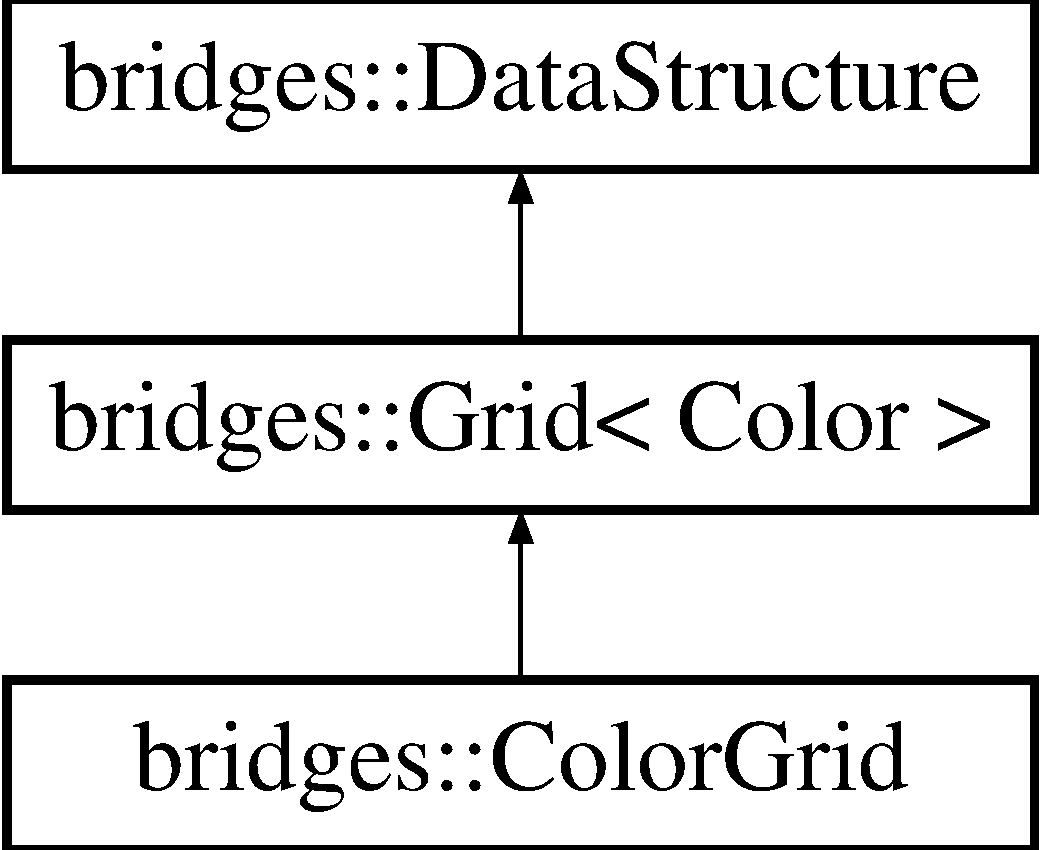
\includegraphics[height=3.000000cm]{classbridges_1_1_color_grid}
\end{center}
\end{figure}
\subsection*{Public Member Functions}
\begin{DoxyCompactItemize}
\item 
virtual const string \hyperlink{classbridges_1_1_color_grid_abe93355089cbae218355529632e3d1fb}{get\+D\+Stype} () const  override
\item 
\hyperlink{classbridges_1_1_color_grid_a00f6ca6b903228b78538a9f0511ffe46}{Color\+Grid} ()
\item 
\hyperlink{classbridges_1_1_color_grid_ac5fb993701683939d96fd7ac6515efc3}{Color\+Grid} (int rows, int cols)
\item 
\hyperlink{classbridges_1_1_color_grid_a4b731632c040f1fb05636127627603d5}{Color\+Grid} (int rows, int cols, \hyperlink{classbridges_1_1_color}{Color} color)
\end{DoxyCompactItemize}
\subsection*{Additional Inherited Members}


\subsection{Constructor \& Destructor Documentation}
\hypertarget{classbridges_1_1_color_grid_a00f6ca6b903228b78538a9f0511ffe46}{}\index{bridges\+::\+Color\+Grid@{bridges\+::\+Color\+Grid}!Color\+Grid@{Color\+Grid}}
\index{Color\+Grid@{Color\+Grid}!bridges\+::\+Color\+Grid@{bridges\+::\+Color\+Grid}}
\subsubsection[{Color\+Grid()}]{\setlength{\rightskip}{0pt plus 5cm}bridges\+::\+Color\+Grid\+::\+Color\+Grid (
\begin{DoxyParamCaption}
{}
\end{DoxyParamCaption}
)\hspace{0.3cm}{\ttfamily [inline]}}\label{classbridges_1_1_color_grid_a00f6ca6b903228b78538a9f0511ffe46}
\hyperlink{classbridges_1_1_color_grid}{Color\+Grid} constructors \hypertarget{classbridges_1_1_color_grid_ac5fb993701683939d96fd7ac6515efc3}{}\index{bridges\+::\+Color\+Grid@{bridges\+::\+Color\+Grid}!Color\+Grid@{Color\+Grid}}
\index{Color\+Grid@{Color\+Grid}!bridges\+::\+Color\+Grid@{bridges\+::\+Color\+Grid}}
\subsubsection[{Color\+Grid(int rows, int cols)}]{\setlength{\rightskip}{0pt plus 5cm}bridges\+::\+Color\+Grid\+::\+Color\+Grid (
\begin{DoxyParamCaption}
\item[{int}]{rows, }
\item[{int}]{cols}
\end{DoxyParamCaption}
)\hspace{0.3cm}{\ttfamily [inline]}}\label{classbridges_1_1_color_grid_ac5fb993701683939d96fd7ac6515efc3}
\hyperlink{classbridges_1_1_grid}{Grid} constructor with size arguments


\begin{DoxyParams}{Parameters}
{\em rows} & -\/ int representing the number of rows of the grid \\
\hline
{\em cols} & -\/ int representing the number of columns of the grid \\
\hline
\end{DoxyParams}
\hypertarget{classbridges_1_1_color_grid_a4b731632c040f1fb05636127627603d5}{}\index{bridges\+::\+Color\+Grid@{bridges\+::\+Color\+Grid}!Color\+Grid@{Color\+Grid}}
\index{Color\+Grid@{Color\+Grid}!bridges\+::\+Color\+Grid@{bridges\+::\+Color\+Grid}}
\subsubsection[{Color\+Grid(int rows, int cols, Color color)}]{\setlength{\rightskip}{0pt plus 5cm}bridges\+::\+Color\+Grid\+::\+Color\+Grid (
\begin{DoxyParamCaption}
\item[{int}]{rows, }
\item[{int}]{cols, }
\item[{{\bf Color}}]{color}
\end{DoxyParamCaption}
)\hspace{0.3cm}{\ttfamily [inline]}}\label{classbridges_1_1_color_grid_a4b731632c040f1fb05636127627603d5}
\hyperlink{classbridges_1_1_grid}{Grid} constructor with size and color string argument


\begin{DoxyParams}{Parameters}
{\em rows} & -\/ int representing the number of rows of the grid \\
\hline
{\em cols} & -\/ int representing the number of columns of the grid \\
\hline
{\em color} & -\/ \hyperlink{classbridges_1_1_color}{Color} object \\
\hline
\end{DoxyParams}


\subsection{Member Function Documentation}
\hypertarget{classbridges_1_1_color_grid_abe93355089cbae218355529632e3d1fb}{}\index{bridges\+::\+Color\+Grid@{bridges\+::\+Color\+Grid}!get\+D\+Stype@{get\+D\+Stype}}
\index{get\+D\+Stype@{get\+D\+Stype}!bridges\+::\+Color\+Grid@{bridges\+::\+Color\+Grid}}
\subsubsection[{get\+D\+Stype() const  override}]{\setlength{\rightskip}{0pt plus 5cm}virtual const string bridges\+::\+Color\+Grid\+::get\+D\+Stype (
\begin{DoxyParamCaption}
{}
\end{DoxyParamCaption}
) const\hspace{0.3cm}{\ttfamily [inline]}, {\ttfamily [override]}, {\ttfamily [virtual]}}\label{classbridges_1_1_color_grid_abe93355089cbae218355529632e3d1fb}
\begin{DoxyReturn}{Returns}
The string representation of this data structure type 
\end{DoxyReturn}


Reimplemented from \hyperlink{classbridges_1_1_grid_a02561695978011f50894938b78969913}{bridges\+::\+Grid$<$ Color $>$}.



The documentation for this class was generated from the following file\+:\begin{DoxyCompactItemize}
\item 
/\+Users/kalpathi/gr/bridges/bridges17/cxx/src/\hyperlink{_color_grid_8h}{Color\+Grid.\+h}\end{DoxyCompactItemize}

\hypertarget{classbridges_1_1_data_structure}{}\section{bridges\+:\+:Data\+Structure Class Reference}
\label{classbridges_1_1_data_structure}\index{bridges\+::\+Data\+Structure@{bridges\+::\+Data\+Structure}}


This is the superclass of all data structure types in B\+R\+I\+D\+G\+E\+S.  




{\ttfamily \#include $<$Data\+Structure.\+h$>$}

Inheritance diagram for bridges\+:\+:Data\+Structure\+:\begin{figure}[H]
\begin{center}
\leavevmode
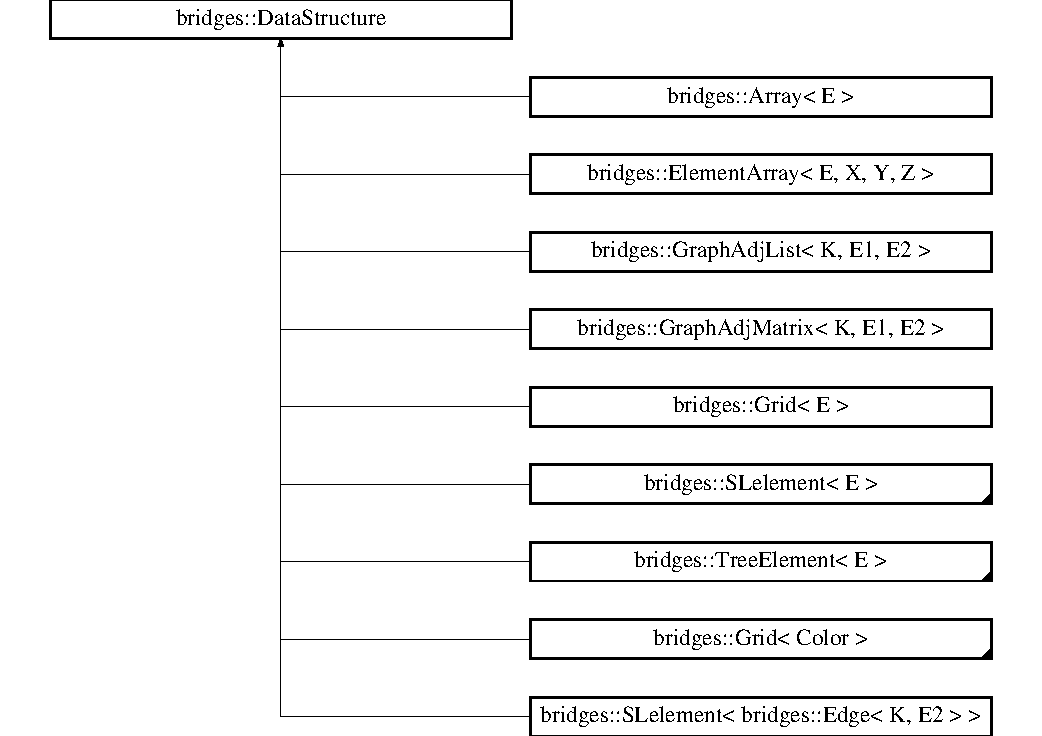
\includegraphics[height=2.594595cm]{classbridges_1_1_data_structure}
\end{center}
\end{figure}
\subsection*{Public Member Functions}
\begin{DoxyCompactItemize}
\item 
virtual \hyperlink{classbridges_1_1_data_structure_afd70a1ae5c2578d80a441714f95f9401}{$\sim$\+Data\+Structure} ()=default
\item 
virtual const string \hyperlink{classbridges_1_1_data_structure_ab6973cdb2a22b7e664b895f1f9c8ad54}{get\+D\+Stype} () const  =0
\item 
virtual void \hyperlink{classbridges_1_1_data_structure_ac3ad75810fd77f0ad35b9b5123d2c8f8}{cleanup} ()
\end{DoxyCompactItemize}
\subsection*{Static Protected Member Functions}
\begin{DoxyCompactItemize}
\item 
static string \hyperlink{classbridges_1_1_data_structure_a2dfc9d9b970680e2b19f7196cf36783a}{remove\+Trailing\+Zeros} (const double \&num)
\end{DoxyCompactItemize}
\subsection*{Friends}
\begin{DoxyCompactItemize}
\item 
class \hyperlink{classbridges_1_1_data_structure_a7f3c8f8f2dfc557bebb6fda1ec6e8ae0}{Bridges\+::\+P\+O\+D}
\end{DoxyCompactItemize}


\subsection{Detailed Description}
This is the superclass of all data structure types in B\+R\+I\+D\+G\+E\+S. 

This is the superclass of all data structure types in B\+R\+I\+D\+G\+E\+S. Both Elements and Graphs inherit from this.

\begin{DoxyDate}{Date}
6/11/15, Dakota Carmer, Kalpathi Subramanian, 7/10/16 
\end{DoxyDate}


\subsection{Constructor \& Destructor Documentation}
\hypertarget{classbridges_1_1_data_structure_afd70a1ae5c2578d80a441714f95f9401}{}\index{bridges\+::\+Data\+Structure@{bridges\+::\+Data\+Structure}!````~Data\+Structure@{$\sim$\+Data\+Structure}}
\index{````~Data\+Structure@{$\sim$\+Data\+Structure}!bridges\+::\+Data\+Structure@{bridges\+::\+Data\+Structure}}
\subsubsection[{$\sim$\+Data\+Structure()=default}]{\setlength{\rightskip}{0pt plus 5cm}virtual bridges\+::\+Data\+Structure\+::$\sim$\+Data\+Structure (
\begin{DoxyParamCaption}
{}
\end{DoxyParamCaption}
)\hspace{0.3cm}{\ttfamily [virtual]}, {\ttfamily [default]}}\label{classbridges_1_1_data_structure_afd70a1ae5c2578d80a441714f95f9401}
Virtual Destructor 

\subsection{Member Function Documentation}
\hypertarget{classbridges_1_1_data_structure_ac3ad75810fd77f0ad35b9b5123d2c8f8}{}\index{bridges\+::\+Data\+Structure@{bridges\+::\+Data\+Structure}!cleanup@{cleanup}}
\index{cleanup@{cleanup}!bridges\+::\+Data\+Structure@{bridges\+::\+Data\+Structure}}
\subsubsection[{cleanup()}]{\setlength{\rightskip}{0pt plus 5cm}virtual void bridges\+::\+Data\+Structure\+::cleanup (
\begin{DoxyParamCaption}
{}
\end{DoxyParamCaption}
)\hspace{0.3cm}{\ttfamily [inline]}, {\ttfamily [virtual]}}\label{classbridges_1_1_data_structure_ac3ad75810fd77f0ad35b9b5123d2c8f8}
Ease of use function for the deletion of an entire datastructure. Overrides should call delete on itself and each linked data structure

\begin{DoxyWarning}{Warning}
Only call if all these data structures were all dynamicaly allocated(aka\+: using new) 
\end{DoxyWarning}


Reimplemented in \hyperlink{classbridges_1_1_tree_element_aad832c9f8dfd7e92c7b06a825f406e1d}{bridges\+::\+Tree\+Element$<$ E $>$}, \hyperlink{classbridges_1_1_s_lelement_ac747648849874407e9d907bb4557dd52}{bridges\+::\+S\+Lelement$<$ E $>$}, and \hyperlink{classbridges_1_1_s_lelement_ac747648849874407e9d907bb4557dd52}{bridges\+::\+S\+Lelement$<$ bridges\+::\+Edge$<$ K $>$ $>$}.

\hypertarget{classbridges_1_1_data_structure_ab6973cdb2a22b7e664b895f1f9c8ad54}{}\index{bridges\+::\+Data\+Structure@{bridges\+::\+Data\+Structure}!get\+D\+Stype@{get\+D\+Stype}}
\index{get\+D\+Stype@{get\+D\+Stype}!bridges\+::\+Data\+Structure@{bridges\+::\+Data\+Structure}}
\subsubsection[{get\+D\+Stype() const  =0}]{\setlength{\rightskip}{0pt plus 5cm}virtual const string bridges\+::\+Data\+Structure\+::get\+D\+Stype (
\begin{DoxyParamCaption}
{}
\end{DoxyParamCaption}
) const\hspace{0.3cm}{\ttfamily [pure virtual]}}\label{classbridges_1_1_data_structure_ab6973cdb2a22b7e664b895f1f9c8ad54}
\begin{DoxyReturn}{Returns}
The string representation of this data structure type 
\end{DoxyReturn}


Implemented in \hyperlink{classbridges_1_1_graph_adj_list_a598803ce2292ce3fa23fbd3f37f12176}{bridges\+::\+Graph\+Adj\+List$<$ K, E $>$}, \hyperlink{classbridges_1_1_element_a9e71af13963e8cc7ec35053797e49155}{bridges\+::\+Element$<$ E $>$}, \hyperlink{classbridges_1_1_element_a9e71af13963e8cc7ec35053797e49155}{bridges\+::\+Element$<$ bridges\+::\+Edge$<$ K $>$ $>$}, \hyperlink{classbridges_1_1_b_s_t_element_a56fdac281f5270446cf7ad98ff6c7a80}{bridges\+::\+B\+S\+T\+Element$<$ K, E $>$}, \hyperlink{classbridges_1_1_d_lelement_a5deee8b106a2f3f7d221152bf244016d}{bridges\+::\+D\+Lelement$<$ E $>$}, \hyperlink{classbridges_1_1_bin_tree_element_ae0bf807e8fd653574d161b4847c92e4e}{bridges\+::\+Bin\+Tree\+Element$<$ E $>$}, \hyperlink{classbridges_1_1_s_lelement_a74aece34b334c1d4318694312d70ce89}{bridges\+::\+S\+Lelement$<$ E $>$}, \hyperlink{classbridges_1_1_s_lelement_a74aece34b334c1d4318694312d70ce89}{bridges\+::\+S\+Lelement$<$ bridges\+::\+Edge$<$ K $>$ $>$}, \hyperlink{classbridges_1_1_a_v_l_tree_element_a408f7c79eb3414b54a8c9bdc6b31d972}{bridges\+::\+A\+V\+L\+Tree\+Element$<$ K, E $>$}, \hyperlink{classbridges_1_1_tree_element_a2990457495ddecc77fa1dda4f47f3010}{bridges\+::\+Tree\+Element$<$ E $>$}, and \hyperlink{classbridges_1_1_graph_adj_matrix_a05a0140f4e9f1a8cfb87e68960daca7e}{bridges\+::\+Graph\+Adj\+Matrix$<$ K, E $>$}.

\hypertarget{classbridges_1_1_data_structure_a2dfc9d9b970680e2b19f7196cf36783a}{}\index{bridges\+::\+Data\+Structure@{bridges\+::\+Data\+Structure}!remove\+Trailing\+Zeros@{remove\+Trailing\+Zeros}}
\index{remove\+Trailing\+Zeros@{remove\+Trailing\+Zeros}!bridges\+::\+Data\+Structure@{bridges\+::\+Data\+Structure}}
\subsubsection[{remove\+Trailing\+Zeros(const double \&num)}]{\setlength{\rightskip}{0pt plus 5cm}static string bridges\+::\+Data\+Structure\+::remove\+Trailing\+Zeros (
\begin{DoxyParamCaption}
\item[{const double \&}]{num}
\end{DoxyParamCaption}
)\hspace{0.3cm}{\ttfamily [inline]}, {\ttfamily [static]}, {\ttfamily [protected]}}\label{classbridges_1_1_data_structure_a2dfc9d9b970680e2b19f7196cf36783a}
\begin{DoxyReturn}{Returns}
to\+\_\+string of \char`\"{}num\char`\"{} without unnessasary trailing 0s 
\end{DoxyReturn}


\subsection{Friends And Related Function Documentation}
\hypertarget{classbridges_1_1_data_structure_a7f3c8f8f2dfc557bebb6fda1ec6e8ae0}{}\index{bridges\+::\+Data\+Structure@{bridges\+::\+Data\+Structure}!Bridges\+::\+P\+O\+D@{Bridges\+::\+P\+O\+D}}
\index{Bridges\+::\+P\+O\+D@{Bridges\+::\+P\+O\+D}!bridges\+::\+Data\+Structure@{bridges\+::\+Data\+Structure}}
\subsubsection[{Bridges\+::\+P\+O\+D}]{\setlength{\rightskip}{0pt plus 5cm}friend class {\bf Bridges\+::\+P\+O\+D}\hspace{0.3cm}{\ttfamily [friend]}}\label{classbridges_1_1_data_structure_a7f3c8f8f2dfc557bebb6fda1ec6e8ae0}


The documentation for this class was generated from the following file\+:\begin{DoxyCompactItemize}
\item 
/\+Users/krs/gr/bridges/cxx/git-\/cxx/src/\hyperlink{_data_structure_8h}{Data\+Structure.\+h}\end{DoxyCompactItemize}

\hypertarget{classbridges_1_1_d_lelement}{}\section{bridges\+:\+:D\+Lelement$<$ E $>$ Class Template Reference}
\label{classbridges_1_1_d_lelement}\index{bridges\+::\+D\+Lelement$<$ E $>$@{bridges\+::\+D\+Lelement$<$ E $>$}}


The doubly linked list element, derived from \hyperlink{classbridges_1_1_s_lelement}{S\+Lelement}.  




{\ttfamily \#include $<$D\+Lelement.\+h$>$}

Inheritance diagram for bridges\+:\+:D\+Lelement$<$ E $>$\+:\begin{figure}[H]
\begin{center}
\leavevmode
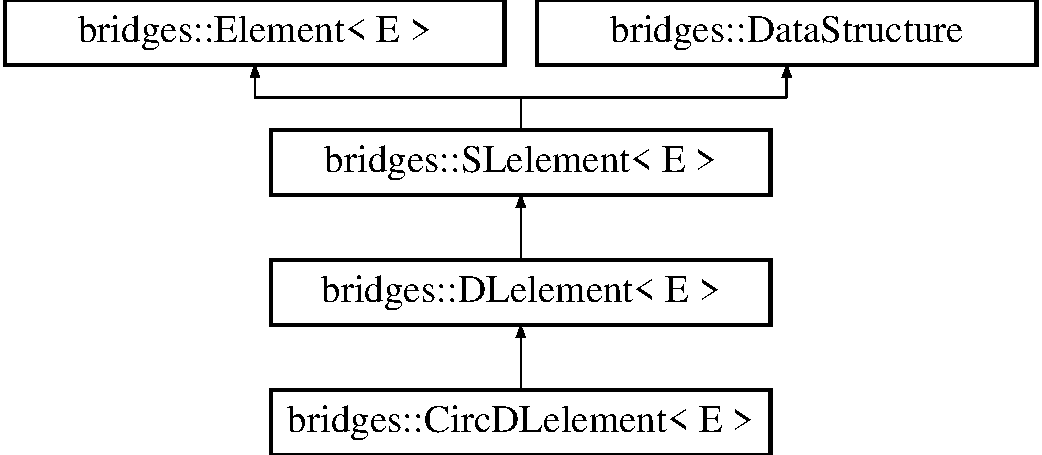
\includegraphics[height=4.000000cm]{classbridges_1_1_d_lelement}
\end{center}
\end{figure}
\subsection*{Public Member Functions}
\begin{DoxyCompactItemize}
\item 
\hyperlink{classbridges_1_1_d_lelement_a846424760c641ba5f496615361d8f79c}{D\+Lelement} (\hyperlink{classbridges_1_1_d_lelement}{D\+Lelement} $\ast$n, \hyperlink{classbridges_1_1_d_lelement}{D\+Lelement} $\ast$p=nullptr, const E \&val=E(), const string \&lab=string())
\item 
\hyperlink{classbridges_1_1_d_lelement_aab0e126bc0b34815f855899b5a8fa75a}{D\+Lelement} (const E \&val=E(), const string \&lab=string())
\item 
virtual const string \hyperlink{classbridges_1_1_d_lelement_a5deee8b106a2f3f7d221152bf244016d}{get\+D\+Stype} () const  override
\item 
virtual \hyperlink{classbridges_1_1_d_lelement}{D\+Lelement} $\ast$ \hyperlink{classbridges_1_1_d_lelement_a0c713707d8c7d0a97fe4194ed6592ede}{get\+Next} () override
\item 
virtual const \hyperlink{classbridges_1_1_d_lelement}{D\+Lelement} $\ast$ \hyperlink{classbridges_1_1_d_lelement_aedf2348136456e0ee116f297f51d7637}{get\+Next} () const  override
\item 
void \hyperlink{classbridges_1_1_d_lelement_aba19c60b1d10c145b1b737f9134f4497}{set\+Next} (\hyperlink{classbridges_1_1_d_lelement}{D\+Lelement} $\ast$n)
\item 
\hyperlink{classbridges_1_1_d_lelement}{D\+Lelement} $\ast$ \hyperlink{classbridges_1_1_d_lelement_a5b0316fb255d022b0dc3065d681fc2a7}{get\+Prev} ()
\item 
const \hyperlink{classbridges_1_1_d_lelement}{D\+Lelement} $\ast$ \hyperlink{classbridges_1_1_d_lelement_a580c05bdafd32a3d6d9d1148b410a7c8}{get\+Prev} () const 
\item 
void \hyperlink{classbridges_1_1_d_lelement_af146e0e10faba6395272d5fc1560f266}{set\+Prev} (\hyperlink{classbridges_1_1_d_lelement}{D\+Lelement} $\ast$p)
\end{DoxyCompactItemize}
\subsection*{Additional Inherited Members}


\subsection{Detailed Description}
\subsubsection*{template$<$typename E$>$class bridges\+::\+D\+Lelement$<$ E $>$}

The doubly linked list element, derived from \hyperlink{classbridges_1_1_s_lelement}{S\+Lelement}. 

This class extends the S\+Lelelement class by adding a previous \hyperlink{classbridges_1_1_d_lelement}{D\+Lelement} pointer

Generic Parameters\+: E the application data type

\begin{DoxyAuthor}{Author}
Kalpathi Subramanian 
\end{DoxyAuthor}
\begin{DoxyDate}{Date}
6/11/15 
\end{DoxyDate}


\subsection{Constructor \& Destructor Documentation}
\hypertarget{classbridges_1_1_d_lelement_a846424760c641ba5f496615361d8f79c}{}\index{bridges\+::\+D\+Lelement@{bridges\+::\+D\+Lelement}!D\+Lelement@{D\+Lelement}}
\index{D\+Lelement@{D\+Lelement}!bridges\+::\+D\+Lelement@{bridges\+::\+D\+Lelement}}
\subsubsection[{D\+Lelement(\+D\+Lelement $\ast$n, D\+Lelement $\ast$p=nullptr, const E \&val=\+E(), const string \&lab=string())}]{\setlength{\rightskip}{0pt plus 5cm}template$<$typename E $>$ {\bf bridges\+::\+D\+Lelement}$<$ E $>$\+::{\bf D\+Lelement} (
\begin{DoxyParamCaption}
\item[{{\bf D\+Lelement}$<$ E $>$ $\ast$}]{n, }
\item[{{\bf D\+Lelement}$<$ E $>$ $\ast$}]{p = {\ttfamily nullptr}, }
\item[{const E \&}]{val = {\ttfamily E()}, }
\item[{const string \&}]{lab = {\ttfamily string()}}
\end{DoxyParamCaption}
)\hspace{0.3cm}{\ttfamily [inline]}}\label{classbridges_1_1_d_lelement_a846424760c641ba5f496615361d8f79c}
Constructs a dlelement with the provided value, label, next and previous dlelements. The defaults will be used if not provided.


\begin{DoxyParams}{Parameters}
{\em val} & The data to hold \\
\hline
{\em lab} & The label to show \\
\hline
{\em n} & The next \hyperlink{classbridges_1_1_d_lelement}{D\+Lelement} \\
\hline
{\em p} & The previous \hyperlink{classbridges_1_1_d_lelement}{D\+Lelement} \\
\hline
\end{DoxyParams}
\hypertarget{classbridges_1_1_d_lelement_aab0e126bc0b34815f855899b5a8fa75a}{}\index{bridges\+::\+D\+Lelement@{bridges\+::\+D\+Lelement}!D\+Lelement@{D\+Lelement}}
\index{D\+Lelement@{D\+Lelement}!bridges\+::\+D\+Lelement@{bridges\+::\+D\+Lelement}}
\subsubsection[{D\+Lelement(const E \&val=\+E(), const string \&lab=string())}]{\setlength{\rightskip}{0pt plus 5cm}template$<$typename E $>$ {\bf bridges\+::\+D\+Lelement}$<$ E $>$\+::{\bf D\+Lelement} (
\begin{DoxyParamCaption}
\item[{const E \&}]{val = {\ttfamily E()}, }
\item[{const string \&}]{lab = {\ttfamily string()}}
\end{DoxyParamCaption}
)\hspace{0.3cm}{\ttfamily [inline]}}\label{classbridges_1_1_d_lelement_aab0e126bc0b34815f855899b5a8fa75a}
Constructs a dlelement with the provided value and label, setting the next and previous dlelements to N\+U\+L\+L. The defaults will be used if not provided.


\begin{DoxyParams}{Parameters}
{\em val} & The data to hold \\
\hline
{\em lab} & The label to show \\
\hline
\end{DoxyParams}


\subsection{Member Function Documentation}
\hypertarget{classbridges_1_1_d_lelement_a5deee8b106a2f3f7d221152bf244016d}{}\index{bridges\+::\+D\+Lelement@{bridges\+::\+D\+Lelement}!get\+D\+Stype@{get\+D\+Stype}}
\index{get\+D\+Stype@{get\+D\+Stype}!bridges\+::\+D\+Lelement@{bridges\+::\+D\+Lelement}}
\subsubsection[{get\+D\+Stype() const  override}]{\setlength{\rightskip}{0pt plus 5cm}template$<$typename E $>$ virtual const string {\bf bridges\+::\+D\+Lelement}$<$ E $>$\+::get\+D\+Stype (
\begin{DoxyParamCaption}
{}
\end{DoxyParamCaption}
) const\hspace{0.3cm}{\ttfamily [inline]}, {\ttfamily [override]}, {\ttfamily [virtual]}}\label{classbridges_1_1_d_lelement_a5deee8b106a2f3f7d221152bf244016d}
Return the data structure type

\begin{DoxyReturn}{Returns}
The string representation of this data structure type 
\end{DoxyReturn}


Reimplemented from \hyperlink{classbridges_1_1_s_lelement_a74aece34b334c1d4318694312d70ce89}{bridges\+::\+S\+Lelement$<$ E $>$}.



Reimplemented in \hyperlink{classbridges_1_1_circ_d_lelement_aa634a40db1541b340c487c6fc9f42b0a}{bridges\+::\+Circ\+D\+Lelement$<$ E $>$}.

\hypertarget{classbridges_1_1_d_lelement_a0c713707d8c7d0a97fe4194ed6592ede}{}\index{bridges\+::\+D\+Lelement@{bridges\+::\+D\+Lelement}!get\+Next@{get\+Next}}
\index{get\+Next@{get\+Next}!bridges\+::\+D\+Lelement@{bridges\+::\+D\+Lelement}}
\subsubsection[{get\+Next() override}]{\setlength{\rightskip}{0pt plus 5cm}template$<$typename E $>$ virtual {\bf D\+Lelement}$\ast$ {\bf bridges\+::\+D\+Lelement}$<$ E $>$\+::get\+Next (
\begin{DoxyParamCaption}
{}
\end{DoxyParamCaption}
)\hspace{0.3cm}{\ttfamily [inline]}, {\ttfamily [override]}, {\ttfamily [virtual]}}\label{classbridges_1_1_d_lelement_a0c713707d8c7d0a97fe4194ed6592ede}
Return the next D\+L element.

\begin{DoxyReturn}{Returns}
The next \hyperlink{classbridges_1_1_d_lelement}{D\+Lelement} 
\end{DoxyReturn}


Reimplemented from \hyperlink{classbridges_1_1_s_lelement_a5bd74108a9aa49339378bf62cdbb19ca}{bridges\+::\+S\+Lelement$<$ E $>$}.



Reimplemented in \hyperlink{classbridges_1_1_circ_d_lelement_a52996d42efc5680d1f8b406143abfee5}{bridges\+::\+Circ\+D\+Lelement$<$ E $>$}.

\hypertarget{classbridges_1_1_d_lelement_aedf2348136456e0ee116f297f51d7637}{}\index{bridges\+::\+D\+Lelement@{bridges\+::\+D\+Lelement}!get\+Next@{get\+Next}}
\index{get\+Next@{get\+Next}!bridges\+::\+D\+Lelement@{bridges\+::\+D\+Lelement}}
\subsubsection[{get\+Next() const  override}]{\setlength{\rightskip}{0pt plus 5cm}template$<$typename E $>$ virtual const {\bf D\+Lelement}$\ast$ {\bf bridges\+::\+D\+Lelement}$<$ E $>$\+::get\+Next (
\begin{DoxyParamCaption}
{}
\end{DoxyParamCaption}
) const\hspace{0.3cm}{\ttfamily [inline]}, {\ttfamily [override]}, {\ttfamily [virtual]}}\label{classbridges_1_1_d_lelement_aedf2348136456e0ee116f297f51d7637}
Constant version

\begin{DoxyReturn}{Returns}
The next \hyperlink{classbridges_1_1_d_lelement}{D\+Lelement} 
\end{DoxyReturn}


Reimplemented from \hyperlink{classbridges_1_1_s_lelement_a1d247f34c384e7ef162148320a4946fe}{bridges\+::\+S\+Lelement$<$ E $>$}.



Reimplemented in \hyperlink{classbridges_1_1_circ_d_lelement_a595c8a0744abc665afb28f264472511a}{bridges\+::\+Circ\+D\+Lelement$<$ E $>$}.

\hypertarget{classbridges_1_1_d_lelement_a5b0316fb255d022b0dc3065d681fc2a7}{}\index{bridges\+::\+D\+Lelement@{bridges\+::\+D\+Lelement}!get\+Prev@{get\+Prev}}
\index{get\+Prev@{get\+Prev}!bridges\+::\+D\+Lelement@{bridges\+::\+D\+Lelement}}
\subsubsection[{get\+Prev()}]{\setlength{\rightskip}{0pt plus 5cm}template$<$typename E $>$ {\bf D\+Lelement}$\ast$ {\bf bridges\+::\+D\+Lelement}$<$ E $>$\+::get\+Prev (
\begin{DoxyParamCaption}
{}
\end{DoxyParamCaption}
)\hspace{0.3cm}{\ttfamily [inline]}}\label{classbridges_1_1_d_lelement_a5b0316fb255d022b0dc3065d681fc2a7}
\begin{DoxyReturn}{Returns}
The previous \hyperlink{classbridges_1_1_d_lelement}{D\+Lelement} 
\end{DoxyReturn}
\hypertarget{classbridges_1_1_d_lelement_a580c05bdafd32a3d6d9d1148b410a7c8}{}\index{bridges\+::\+D\+Lelement@{bridges\+::\+D\+Lelement}!get\+Prev@{get\+Prev}}
\index{get\+Prev@{get\+Prev}!bridges\+::\+D\+Lelement@{bridges\+::\+D\+Lelement}}
\subsubsection[{get\+Prev() const }]{\setlength{\rightskip}{0pt plus 5cm}template$<$typename E $>$ const {\bf D\+Lelement}$\ast$ {\bf bridges\+::\+D\+Lelement}$<$ E $>$\+::get\+Prev (
\begin{DoxyParamCaption}
{}
\end{DoxyParamCaption}
) const\hspace{0.3cm}{\ttfamily [inline]}}\label{classbridges_1_1_d_lelement_a580c05bdafd32a3d6d9d1148b410a7c8}
Constant version

\begin{DoxyReturn}{Returns}
The previous \hyperlink{classbridges_1_1_d_lelement}{D\+Lelement} 
\end{DoxyReturn}
\hypertarget{classbridges_1_1_d_lelement_aba19c60b1d10c145b1b737f9134f4497}{}\index{bridges\+::\+D\+Lelement@{bridges\+::\+D\+Lelement}!set\+Next@{set\+Next}}
\index{set\+Next@{set\+Next}!bridges\+::\+D\+Lelement@{bridges\+::\+D\+Lelement}}
\subsubsection[{set\+Next(\+D\+Lelement $\ast$n)}]{\setlength{\rightskip}{0pt plus 5cm}template$<$typename E $>$ void {\bf bridges\+::\+D\+Lelement}$<$ E $>$\+::set\+Next (
\begin{DoxyParamCaption}
\item[{{\bf D\+Lelement}$<$ E $>$ $\ast$}]{n}
\end{DoxyParamCaption}
)\hspace{0.3cm}{\ttfamily [inline]}}\label{classbridges_1_1_d_lelement_aba19c60b1d10c145b1b737f9134f4497}
Sets next to \char`\"{}n\char`\"{}


\begin{DoxyParams}{Parameters}
{\em n} & The next \hyperlink{classbridges_1_1_d_lelement}{D\+Lelement} \\
\hline
\end{DoxyParams}
\hypertarget{classbridges_1_1_d_lelement_af146e0e10faba6395272d5fc1560f266}{}\index{bridges\+::\+D\+Lelement@{bridges\+::\+D\+Lelement}!set\+Prev@{set\+Prev}}
\index{set\+Prev@{set\+Prev}!bridges\+::\+D\+Lelement@{bridges\+::\+D\+Lelement}}
\subsubsection[{set\+Prev(\+D\+Lelement $\ast$p)}]{\setlength{\rightskip}{0pt plus 5cm}template$<$typename E $>$ void {\bf bridges\+::\+D\+Lelement}$<$ E $>$\+::set\+Prev (
\begin{DoxyParamCaption}
\item[{{\bf D\+Lelement}$<$ E $>$ $\ast$}]{p}
\end{DoxyParamCaption}
)\hspace{0.3cm}{\ttfamily [inline]}}\label{classbridges_1_1_d_lelement_af146e0e10faba6395272d5fc1560f266}
Sets prev to \char`\"{}p\char`\"{}


\begin{DoxyParams}{Parameters}
{\em p} & The previous \hyperlink{classbridges_1_1_d_lelement}{D\+Lelement} \\
\hline
\end{DoxyParams}


The documentation for this class was generated from the following file\+:\begin{DoxyCompactItemize}
\item 
/\+Users/krs/gr/bridges/bridges17/cxx/src/\hyperlink{_d_lelement_8h}{D\+Lelement.\+h}\end{DoxyCompactItemize}

\hypertarget{classbridges_1_1_earthquake_u_s_g_s}{}\section{bridges\+:\+:Earthquake\+U\+S\+G\+S Class Reference}
\label{classbridges_1_1_earthquake_u_s_g_s}\index{bridges\+::\+Earthquake\+U\+S\+G\+S@{bridges\+::\+Earthquake\+U\+S\+G\+S}}


Class that hold earthquake data, for use with U\+S\+G\+I\+S retrieved quake data.  




{\ttfamily \#include $<$Earthquake\+U\+S\+G\+S.\+h$>$}

\subsection*{Public Member Functions}
\begin{DoxyCompactItemize}
\item 
\hyperlink{classbridges_1_1_earthquake_u_s_g_s_a540ae74c248da179fbbd182b843a14e0}{Earthquake\+U\+S\+G\+S} ()
\item 
\hyperlink{classbridges_1_1_earthquake_u_s_g_s_a9c7f7aec2ddc173660a7015b90c7b7b0}{Earthquake\+U\+S\+G\+S} (double magnitude, double longit, double latit, string location, string title, string url, string time)
\item 
\hyperlink{classbridges_1_1_earthquake_u_s_g_s_aa52d05b3119c6a4e45867dc4aaeba59e}{Earthquake\+U\+S\+G\+S} (\hyperlink{classbridges_1_1_earthquake_u_s_g_s}{Earthquake\+U\+S\+G\+S} $\ast$eq)
\item 
string \hyperlink{classbridges_1_1_earthquake_u_s_g_s_af8230252cb495e2c87bdd0ed1fbd609f}{get\+Time} () const 
\item 
string \hyperlink{classbridges_1_1_earthquake_u_s_g_s_a74d02315dd50f0d41d0340655c700aff}{get\+Date\+Str} () const 
\item 
void \hyperlink{classbridges_1_1_earthquake_u_s_g_s_a70d79cd5c3666b8a32b1d45d7364054b}{set\+Time} (string tm)
\item 
int \hyperlink{classbridges_1_1_earthquake_u_s_g_s_af82196433d7fc04e309e37d902706c8d}{get\+Year} () const 
\item 
int \hyperlink{classbridges_1_1_earthquake_u_s_g_s_a9d9a998b0092f59e9b45a9c0af715813}{get\+Month} () const 
\item 
int \hyperlink{classbridges_1_1_earthquake_u_s_g_s_a469f812e467023eb9dceaa1519c8f8b8}{get\+Day} () const 
\item 
int \hyperlink{classbridges_1_1_earthquake_u_s_g_s_a2c0989152166d3ec0d3cc7feab7e9093}{get\+Hour} () const 
\item 
int \hyperlink{classbridges_1_1_earthquake_u_s_g_s_aa85673b9c3e8fdeedfd3ed9ae38507e2}{get\+Minutes} () const 
\item 
int \hyperlink{classbridges_1_1_earthquake_u_s_g_s_a73486c57f8f9e4b6cedce1907fb5ae0a}{get\+Seconds} () const 
\item 
float \hyperlink{classbridges_1_1_earthquake_u_s_g_s_a0bc39612708b8333f7c03500ccc6d614}{get\+Latit} () const 
\item 
void \hyperlink{classbridges_1_1_earthquake_u_s_g_s_a143678bb9dd697f82dcb260ddab78f82}{set\+Latit} (float latit)
\item 
float \hyperlink{classbridges_1_1_earthquake_u_s_g_s_a4387cf6d8ea0922558cb07fbd9d5b23e}{get\+Longit} () const 
\item 
void \hyperlink{classbridges_1_1_earthquake_u_s_g_s_a745dc27f3c68a3ae996ceb7771d89ec5}{set\+Longit} (float longit)
\item 
string \hyperlink{classbridges_1_1_earthquake_u_s_g_s_a63bf958e1ac2b6b4797c1733b33c4463}{get\+Location} () const 
\item 
void \hyperlink{classbridges_1_1_earthquake_u_s_g_s_a5dc533759cc900440d70bdfc68f16599}{set\+Location} (string location)
\item 
string \hyperlink{classbridges_1_1_earthquake_u_s_g_s_ab0ecd24e7a2679919b53d3fa27d7429c}{get\+Title} () const 
\item 
void \hyperlink{classbridges_1_1_earthquake_u_s_g_s_a78fe86dcb1bae8470d5ac58fdda2fe51}{set\+Title} (string title)
\item 
string \hyperlink{classbridges_1_1_earthquake_u_s_g_s_a0a82972d7f72a10fd5899dcc26715a9d}{get\+Url} () const 
\item 
void \hyperlink{classbridges_1_1_earthquake_u_s_g_s_ac07298c50e03955d167a2ca38c5150be}{set\+Url} (string url)
\item 
double \hyperlink{classbridges_1_1_earthquake_u_s_g_s_a4e28322b7c9585c7bf56876c52693565}{get\+Magnitude} () const 
\item 
void \hyperlink{classbridges_1_1_earthquake_u_s_g_s_aae8be6112f5c27c168c452261d9b29a2}{set\+Magnitude} (double magnitude)
\end{DoxyCompactItemize}


\subsection{Detailed Description}
Class that hold earthquake data, for use with U\+S\+G\+I\+S retrieved quake data. 

Class that holds earthquake U\+S\+G\+I\+S data. B\+R\+I\+D\+G\+E\+S uses scripts to continually monitor U\+S\+G\+I\+S site (tweets) and retrieve the latest quake data for use in student projects.

Kalpathi Subramanian, 2/18/18 

\subsection{Constructor \& Destructor Documentation}
\hypertarget{classbridges_1_1_earthquake_u_s_g_s_a540ae74c248da179fbbd182b843a14e0}{}\index{bridges\+::\+Earthquake\+U\+S\+G\+S@{bridges\+::\+Earthquake\+U\+S\+G\+S}!Earthquake\+U\+S\+G\+S@{Earthquake\+U\+S\+G\+S}}
\index{Earthquake\+U\+S\+G\+S@{Earthquake\+U\+S\+G\+S}!bridges\+::\+Earthquake\+U\+S\+G\+S@{bridges\+::\+Earthquake\+U\+S\+G\+S}}
\subsubsection[{Earthquake\+U\+S\+G\+S()}]{\setlength{\rightskip}{0pt plus 5cm}bridges\+::\+Earthquake\+U\+S\+G\+S\+::\+Earthquake\+U\+S\+G\+S (
\begin{DoxyParamCaption}
{}
\end{DoxyParamCaption}
)\hspace{0.3cm}{\ttfamily [inline]}}\label{classbridges_1_1_earthquake_u_s_g_s_a540ae74c248da179fbbd182b843a14e0}
\hypertarget{classbridges_1_1_earthquake_u_s_g_s_a9c7f7aec2ddc173660a7015b90c7b7b0}{}\index{bridges\+::\+Earthquake\+U\+S\+G\+S@{bridges\+::\+Earthquake\+U\+S\+G\+S}!Earthquake\+U\+S\+G\+S@{Earthquake\+U\+S\+G\+S}}
\index{Earthquake\+U\+S\+G\+S@{Earthquake\+U\+S\+G\+S}!bridges\+::\+Earthquake\+U\+S\+G\+S@{bridges\+::\+Earthquake\+U\+S\+G\+S}}
\subsubsection[{Earthquake\+U\+S\+G\+S(double magnitude, double longit, double latit, string location, string title, string url, string time)}]{\setlength{\rightskip}{0pt plus 5cm}bridges\+::\+Earthquake\+U\+S\+G\+S\+::\+Earthquake\+U\+S\+G\+S (
\begin{DoxyParamCaption}
\item[{double}]{magnitude, }
\item[{double}]{longit, }
\item[{double}]{latit, }
\item[{string}]{location, }
\item[{string}]{title, }
\item[{string}]{url, }
\item[{string}]{time}
\end{DoxyParamCaption}
)\hspace{0.3cm}{\ttfamily [inline]}}\label{classbridges_1_1_earthquake_u_s_g_s_a9c7f7aec2ddc173660a7015b90c7b7b0}
\hypertarget{classbridges_1_1_earthquake_u_s_g_s_aa52d05b3119c6a4e45867dc4aaeba59e}{}\index{bridges\+::\+Earthquake\+U\+S\+G\+S@{bridges\+::\+Earthquake\+U\+S\+G\+S}!Earthquake\+U\+S\+G\+S@{Earthquake\+U\+S\+G\+S}}
\index{Earthquake\+U\+S\+G\+S@{Earthquake\+U\+S\+G\+S}!bridges\+::\+Earthquake\+U\+S\+G\+S@{bridges\+::\+Earthquake\+U\+S\+G\+S}}
\subsubsection[{Earthquake\+U\+S\+G\+S(\+Earthquake\+U\+S\+G\+S $\ast$eq)}]{\setlength{\rightskip}{0pt plus 5cm}bridges\+::\+Earthquake\+U\+S\+G\+S\+::\+Earthquake\+U\+S\+G\+S (
\begin{DoxyParamCaption}
\item[{{\bf Earthquake\+U\+S\+G\+S} $\ast$}]{eq}
\end{DoxyParamCaption}
)\hspace{0.3cm}{\ttfamily [inline]}}\label{classbridges_1_1_earthquake_u_s_g_s_aa52d05b3119c6a4e45867dc4aaeba59e}


\subsection{Member Function Documentation}
\hypertarget{classbridges_1_1_earthquake_u_s_g_s_a74d02315dd50f0d41d0340655c700aff}{}\index{bridges\+::\+Earthquake\+U\+S\+G\+S@{bridges\+::\+Earthquake\+U\+S\+G\+S}!get\+Date\+Str@{get\+Date\+Str}}
\index{get\+Date\+Str@{get\+Date\+Str}!bridges\+::\+Earthquake\+U\+S\+G\+S@{bridges\+::\+Earthquake\+U\+S\+G\+S}}
\subsubsection[{get\+Date\+Str() const }]{\setlength{\rightskip}{0pt plus 5cm}string bridges\+::\+Earthquake\+U\+S\+G\+S\+::get\+Date\+Str (
\begin{DoxyParamCaption}
{}
\end{DoxyParamCaption}
) const\hspace{0.3cm}{\ttfamily [inline]}}\label{classbridges_1_1_earthquake_u_s_g_s_a74d02315dd50f0d41d0340655c700aff}
returns the real date in a string format

\begin{DoxyReturn}{Returns}
string 
\end{DoxyReturn}
\hypertarget{classbridges_1_1_earthquake_u_s_g_s_a469f812e467023eb9dceaa1519c8f8b8}{}\index{bridges\+::\+Earthquake\+U\+S\+G\+S@{bridges\+::\+Earthquake\+U\+S\+G\+S}!get\+Day@{get\+Day}}
\index{get\+Day@{get\+Day}!bridges\+::\+Earthquake\+U\+S\+G\+S@{bridges\+::\+Earthquake\+U\+S\+G\+S}}
\subsubsection[{get\+Day() const }]{\setlength{\rightskip}{0pt plus 5cm}int bridges\+::\+Earthquake\+U\+S\+G\+S\+::get\+Day (
\begin{DoxyParamCaption}
{}
\end{DoxyParamCaption}
) const\hspace{0.3cm}{\ttfamily [inline]}}\label{classbridges_1_1_earthquake_u_s_g_s_a469f812e467023eb9dceaa1519c8f8b8}
get day of quake

\begin{DoxyReturn}{Returns}
(int) 
\end{DoxyReturn}
\hypertarget{classbridges_1_1_earthquake_u_s_g_s_a2c0989152166d3ec0d3cc7feab7e9093}{}\index{bridges\+::\+Earthquake\+U\+S\+G\+S@{bridges\+::\+Earthquake\+U\+S\+G\+S}!get\+Hour@{get\+Hour}}
\index{get\+Hour@{get\+Hour}!bridges\+::\+Earthquake\+U\+S\+G\+S@{bridges\+::\+Earthquake\+U\+S\+G\+S}}
\subsubsection[{get\+Hour() const }]{\setlength{\rightskip}{0pt plus 5cm}int bridges\+::\+Earthquake\+U\+S\+G\+S\+::get\+Hour (
\begin{DoxyParamCaption}
{}
\end{DoxyParamCaption}
) const\hspace{0.3cm}{\ttfamily [inline]}}\label{classbridges_1_1_earthquake_u_s_g_s_a2c0989152166d3ec0d3cc7feab7e9093}
get hour of quake

\begin{DoxyReturn}{Returns}
(int) 
\end{DoxyReturn}
\hypertarget{classbridges_1_1_earthquake_u_s_g_s_a0bc39612708b8333f7c03500ccc6d614}{}\index{bridges\+::\+Earthquake\+U\+S\+G\+S@{bridges\+::\+Earthquake\+U\+S\+G\+S}!get\+Latit@{get\+Latit}}
\index{get\+Latit@{get\+Latit}!bridges\+::\+Earthquake\+U\+S\+G\+S@{bridges\+::\+Earthquake\+U\+S\+G\+S}}
\subsubsection[{get\+Latit() const }]{\setlength{\rightskip}{0pt plus 5cm}float bridges\+::\+Earthquake\+U\+S\+G\+S\+::get\+Latit (
\begin{DoxyParamCaption}
{}
\end{DoxyParamCaption}
) const\hspace{0.3cm}{\ttfamily [inline]}}\label{classbridges_1_1_earthquake_u_s_g_s_a0bc39612708b8333f7c03500ccc6d614}
get latitude of quake

\begin{DoxyReturn}{Returns}
(float) 
\end{DoxyReturn}
\hypertarget{classbridges_1_1_earthquake_u_s_g_s_a63bf958e1ac2b6b4797c1733b33c4463}{}\index{bridges\+::\+Earthquake\+U\+S\+G\+S@{bridges\+::\+Earthquake\+U\+S\+G\+S}!get\+Location@{get\+Location}}
\index{get\+Location@{get\+Location}!bridges\+::\+Earthquake\+U\+S\+G\+S@{bridges\+::\+Earthquake\+U\+S\+G\+S}}
\subsubsection[{get\+Location() const }]{\setlength{\rightskip}{0pt plus 5cm}string bridges\+::\+Earthquake\+U\+S\+G\+S\+::get\+Location (
\begin{DoxyParamCaption}
{}
\end{DoxyParamCaption}
) const\hspace{0.3cm}{\ttfamily [inline]}}\label{classbridges_1_1_earthquake_u_s_g_s_a63bf958e1ac2b6b4797c1733b33c4463}
get quake location

\begin{DoxyReturn}{Returns}
(string) 
\end{DoxyReturn}
\hypertarget{classbridges_1_1_earthquake_u_s_g_s_a4387cf6d8ea0922558cb07fbd9d5b23e}{}\index{bridges\+::\+Earthquake\+U\+S\+G\+S@{bridges\+::\+Earthquake\+U\+S\+G\+S}!get\+Longit@{get\+Longit}}
\index{get\+Longit@{get\+Longit}!bridges\+::\+Earthquake\+U\+S\+G\+S@{bridges\+::\+Earthquake\+U\+S\+G\+S}}
\subsubsection[{get\+Longit() const }]{\setlength{\rightskip}{0pt plus 5cm}float bridges\+::\+Earthquake\+U\+S\+G\+S\+::get\+Longit (
\begin{DoxyParamCaption}
{}
\end{DoxyParamCaption}
) const\hspace{0.3cm}{\ttfamily [inline]}}\label{classbridges_1_1_earthquake_u_s_g_s_a4387cf6d8ea0922558cb07fbd9d5b23e}
get longitude of quake location

\begin{DoxyReturn}{Returns}
(float) 
\end{DoxyReturn}
\hypertarget{classbridges_1_1_earthquake_u_s_g_s_a4e28322b7c9585c7bf56876c52693565}{}\index{bridges\+::\+Earthquake\+U\+S\+G\+S@{bridges\+::\+Earthquake\+U\+S\+G\+S}!get\+Magnitude@{get\+Magnitude}}
\index{get\+Magnitude@{get\+Magnitude}!bridges\+::\+Earthquake\+U\+S\+G\+S@{bridges\+::\+Earthquake\+U\+S\+G\+S}}
\subsubsection[{get\+Magnitude() const }]{\setlength{\rightskip}{0pt plus 5cm}double bridges\+::\+Earthquake\+U\+S\+G\+S\+::get\+Magnitude (
\begin{DoxyParamCaption}
{}
\end{DoxyParamCaption}
) const\hspace{0.3cm}{\ttfamily [inline]}}\label{classbridges_1_1_earthquake_u_s_g_s_a4e28322b7c9585c7bf56876c52693565}
get quake magnitude

\begin{DoxyReturn}{Returns}
(double) 
\end{DoxyReturn}
\hypertarget{classbridges_1_1_earthquake_u_s_g_s_aa85673b9c3e8fdeedfd3ed9ae38507e2}{}\index{bridges\+::\+Earthquake\+U\+S\+G\+S@{bridges\+::\+Earthquake\+U\+S\+G\+S}!get\+Minutes@{get\+Minutes}}
\index{get\+Minutes@{get\+Minutes}!bridges\+::\+Earthquake\+U\+S\+G\+S@{bridges\+::\+Earthquake\+U\+S\+G\+S}}
\subsubsection[{get\+Minutes() const }]{\setlength{\rightskip}{0pt plus 5cm}int bridges\+::\+Earthquake\+U\+S\+G\+S\+::get\+Minutes (
\begin{DoxyParamCaption}
{}
\end{DoxyParamCaption}
) const\hspace{0.3cm}{\ttfamily [inline]}}\label{classbridges_1_1_earthquake_u_s_g_s_aa85673b9c3e8fdeedfd3ed9ae38507e2}
get minutes of quake

\begin{DoxyReturn}{Returns}
(int) 
\end{DoxyReturn}
\hypertarget{classbridges_1_1_earthquake_u_s_g_s_a9d9a998b0092f59e9b45a9c0af715813}{}\index{bridges\+::\+Earthquake\+U\+S\+G\+S@{bridges\+::\+Earthquake\+U\+S\+G\+S}!get\+Month@{get\+Month}}
\index{get\+Month@{get\+Month}!bridges\+::\+Earthquake\+U\+S\+G\+S@{bridges\+::\+Earthquake\+U\+S\+G\+S}}
\subsubsection[{get\+Month() const }]{\setlength{\rightskip}{0pt plus 5cm}int bridges\+::\+Earthquake\+U\+S\+G\+S\+::get\+Month (
\begin{DoxyParamCaption}
{}
\end{DoxyParamCaption}
) const\hspace{0.3cm}{\ttfamily [inline]}}\label{classbridges_1_1_earthquake_u_s_g_s_a9d9a998b0092f59e9b45a9c0af715813}
get month of quake

\begin{DoxyReturn}{Returns}
(int) 
\end{DoxyReturn}
\hypertarget{classbridges_1_1_earthquake_u_s_g_s_a73486c57f8f9e4b6cedce1907fb5ae0a}{}\index{bridges\+::\+Earthquake\+U\+S\+G\+S@{bridges\+::\+Earthquake\+U\+S\+G\+S}!get\+Seconds@{get\+Seconds}}
\index{get\+Seconds@{get\+Seconds}!bridges\+::\+Earthquake\+U\+S\+G\+S@{bridges\+::\+Earthquake\+U\+S\+G\+S}}
\subsubsection[{get\+Seconds() const }]{\setlength{\rightskip}{0pt plus 5cm}int bridges\+::\+Earthquake\+U\+S\+G\+S\+::get\+Seconds (
\begin{DoxyParamCaption}
{}
\end{DoxyParamCaption}
) const\hspace{0.3cm}{\ttfamily [inline]}}\label{classbridges_1_1_earthquake_u_s_g_s_a73486c57f8f9e4b6cedce1907fb5ae0a}
get seconds of quake

\begin{DoxyReturn}{Returns}
(int) 
\end{DoxyReturn}
\hypertarget{classbridges_1_1_earthquake_u_s_g_s_af8230252cb495e2c87bdd0ed1fbd609f}{}\index{bridges\+::\+Earthquake\+U\+S\+G\+S@{bridges\+::\+Earthquake\+U\+S\+G\+S}!get\+Time@{get\+Time}}
\index{get\+Time@{get\+Time}!bridges\+::\+Earthquake\+U\+S\+G\+S@{bridges\+::\+Earthquake\+U\+S\+G\+S}}
\subsubsection[{get\+Time() const }]{\setlength{\rightskip}{0pt plus 5cm}string bridges\+::\+Earthquake\+U\+S\+G\+S\+::get\+Time (
\begin{DoxyParamCaption}
{}
\end{DoxyParamCaption}
) const\hspace{0.3cm}{\ttfamily [inline]}}\label{classbridges_1_1_earthquake_u_s_g_s_af8230252cb495e2c87bdd0ed1fbd609f}
return the epoch time of the quake

\begin{DoxyReturn}{Returns}
string 
\end{DoxyReturn}
\hypertarget{classbridges_1_1_earthquake_u_s_g_s_ab0ecd24e7a2679919b53d3fa27d7429c}{}\index{bridges\+::\+Earthquake\+U\+S\+G\+S@{bridges\+::\+Earthquake\+U\+S\+G\+S}!get\+Title@{get\+Title}}
\index{get\+Title@{get\+Title}!bridges\+::\+Earthquake\+U\+S\+G\+S@{bridges\+::\+Earthquake\+U\+S\+G\+S}}
\subsubsection[{get\+Title() const }]{\setlength{\rightskip}{0pt plus 5cm}string bridges\+::\+Earthquake\+U\+S\+G\+S\+::get\+Title (
\begin{DoxyParamCaption}
{}
\end{DoxyParamCaption}
) const\hspace{0.3cm}{\ttfamily [inline]}}\label{classbridges_1_1_earthquake_u_s_g_s_ab0ecd24e7a2679919b53d3fa27d7429c}
get quake title

\begin{DoxyReturn}{Returns}
(string) 
\end{DoxyReturn}
\hypertarget{classbridges_1_1_earthquake_u_s_g_s_a0a82972d7f72a10fd5899dcc26715a9d}{}\index{bridges\+::\+Earthquake\+U\+S\+G\+S@{bridges\+::\+Earthquake\+U\+S\+G\+S}!get\+Url@{get\+Url}}
\index{get\+Url@{get\+Url}!bridges\+::\+Earthquake\+U\+S\+G\+S@{bridges\+::\+Earthquake\+U\+S\+G\+S}}
\subsubsection[{get\+Url() const }]{\setlength{\rightskip}{0pt plus 5cm}string bridges\+::\+Earthquake\+U\+S\+G\+S\+::get\+Url (
\begin{DoxyParamCaption}
{}
\end{DoxyParamCaption}
) const\hspace{0.3cm}{\ttfamily [inline]}}\label{classbridges_1_1_earthquake_u_s_g_s_a0a82972d7f72a10fd5899dcc26715a9d}
get quake url

\begin{DoxyReturn}{Returns}
(string) 
\end{DoxyReturn}
\hypertarget{classbridges_1_1_earthquake_u_s_g_s_af82196433d7fc04e309e37d902706c8d}{}\index{bridges\+::\+Earthquake\+U\+S\+G\+S@{bridges\+::\+Earthquake\+U\+S\+G\+S}!get\+Year@{get\+Year}}
\index{get\+Year@{get\+Year}!bridges\+::\+Earthquake\+U\+S\+G\+S@{bridges\+::\+Earthquake\+U\+S\+G\+S}}
\subsubsection[{get\+Year() const }]{\setlength{\rightskip}{0pt plus 5cm}int bridges\+::\+Earthquake\+U\+S\+G\+S\+::get\+Year (
\begin{DoxyParamCaption}
{}
\end{DoxyParamCaption}
) const\hspace{0.3cm}{\ttfamily [inline]}}\label{classbridges_1_1_earthquake_u_s_g_s_af82196433d7fc04e309e37d902706c8d}
get year of quake

\begin{DoxyReturn}{Returns}
(int) 
\end{DoxyReturn}
\hypertarget{classbridges_1_1_earthquake_u_s_g_s_a143678bb9dd697f82dcb260ddab78f82}{}\index{bridges\+::\+Earthquake\+U\+S\+G\+S@{bridges\+::\+Earthquake\+U\+S\+G\+S}!set\+Latit@{set\+Latit}}
\index{set\+Latit@{set\+Latit}!bridges\+::\+Earthquake\+U\+S\+G\+S@{bridges\+::\+Earthquake\+U\+S\+G\+S}}
\subsubsection[{set\+Latit(float latit)}]{\setlength{\rightskip}{0pt plus 5cm}void bridges\+::\+Earthquake\+U\+S\+G\+S\+::set\+Latit (
\begin{DoxyParamCaption}
\item[{float}]{latit}
\end{DoxyParamCaption}
)\hspace{0.3cm}{\ttfamily [inline]}}\label{classbridges_1_1_earthquake_u_s_g_s_a143678bb9dd697f82dcb260ddab78f82}
set latitude


\begin{DoxyParams}{Parameters}
{\em (float)} & \\
\hline
\end{DoxyParams}
\hypertarget{classbridges_1_1_earthquake_u_s_g_s_a5dc533759cc900440d70bdfc68f16599}{}\index{bridges\+::\+Earthquake\+U\+S\+G\+S@{bridges\+::\+Earthquake\+U\+S\+G\+S}!set\+Location@{set\+Location}}
\index{set\+Location@{set\+Location}!bridges\+::\+Earthquake\+U\+S\+G\+S@{bridges\+::\+Earthquake\+U\+S\+G\+S}}
\subsubsection[{set\+Location(string location)}]{\setlength{\rightskip}{0pt plus 5cm}void bridges\+::\+Earthquake\+U\+S\+G\+S\+::set\+Location (
\begin{DoxyParamCaption}
\item[{string}]{location}
\end{DoxyParamCaption}
)\hspace{0.3cm}{\ttfamily [inline]}}\label{classbridges_1_1_earthquake_u_s_g_s_a5dc533759cc900440d70bdfc68f16599}
set quake location (string)


\begin{DoxyParams}{Parameters}
{\em (string)} & \\
\hline
\end{DoxyParams}
\hypertarget{classbridges_1_1_earthquake_u_s_g_s_a745dc27f3c68a3ae996ceb7771d89ec5}{}\index{bridges\+::\+Earthquake\+U\+S\+G\+S@{bridges\+::\+Earthquake\+U\+S\+G\+S}!set\+Longit@{set\+Longit}}
\index{set\+Longit@{set\+Longit}!bridges\+::\+Earthquake\+U\+S\+G\+S@{bridges\+::\+Earthquake\+U\+S\+G\+S}}
\subsubsection[{set\+Longit(float longit)}]{\setlength{\rightskip}{0pt plus 5cm}void bridges\+::\+Earthquake\+U\+S\+G\+S\+::set\+Longit (
\begin{DoxyParamCaption}
\item[{float}]{longit}
\end{DoxyParamCaption}
)\hspace{0.3cm}{\ttfamily [inline]}}\label{classbridges_1_1_earthquake_u_s_g_s_a745dc27f3c68a3ae996ceb7771d89ec5}
set longitude of quake location


\begin{DoxyParams}{Parameters}
{\em (float)} & \\
\hline
\end{DoxyParams}
\hypertarget{classbridges_1_1_earthquake_u_s_g_s_aae8be6112f5c27c168c452261d9b29a2}{}\index{bridges\+::\+Earthquake\+U\+S\+G\+S@{bridges\+::\+Earthquake\+U\+S\+G\+S}!set\+Magnitude@{set\+Magnitude}}
\index{set\+Magnitude@{set\+Magnitude}!bridges\+::\+Earthquake\+U\+S\+G\+S@{bridges\+::\+Earthquake\+U\+S\+G\+S}}
\subsubsection[{set\+Magnitude(double magnitude)}]{\setlength{\rightskip}{0pt plus 5cm}void bridges\+::\+Earthquake\+U\+S\+G\+S\+::set\+Magnitude (
\begin{DoxyParamCaption}
\item[{double}]{magnitude}
\end{DoxyParamCaption}
)\hspace{0.3cm}{\ttfamily [inline]}}\label{classbridges_1_1_earthquake_u_s_g_s_aae8be6112f5c27c168c452261d9b29a2}
set quake magnitude (double)


\begin{DoxyParams}{Parameters}
{\em (string)} & \\
\hline
\end{DoxyParams}
\hypertarget{classbridges_1_1_earthquake_u_s_g_s_a70d79cd5c3666b8a32b1d45d7364054b}{}\index{bridges\+::\+Earthquake\+U\+S\+G\+S@{bridges\+::\+Earthquake\+U\+S\+G\+S}!set\+Time@{set\+Time}}
\index{set\+Time@{set\+Time}!bridges\+::\+Earthquake\+U\+S\+G\+S@{bridges\+::\+Earthquake\+U\+S\+G\+S}}
\subsubsection[{set\+Time(string tm)}]{\setlength{\rightskip}{0pt plus 5cm}void bridges\+::\+Earthquake\+U\+S\+G\+S\+::set\+Time (
\begin{DoxyParamCaption}
\item[{string}]{tm}
\end{DoxyParamCaption}
)\hspace{0.3cm}{\ttfamily [inline]}}\label{classbridges_1_1_earthquake_u_s_g_s_a70d79cd5c3666b8a32b1d45d7364054b}
set epoch time


\begin{DoxyParams}{Parameters}
{\em tm} & (string) \\
\hline
\end{DoxyParams}
\hypertarget{classbridges_1_1_earthquake_u_s_g_s_a78fe86dcb1bae8470d5ac58fdda2fe51}{}\index{bridges\+::\+Earthquake\+U\+S\+G\+S@{bridges\+::\+Earthquake\+U\+S\+G\+S}!set\+Title@{set\+Title}}
\index{set\+Title@{set\+Title}!bridges\+::\+Earthquake\+U\+S\+G\+S@{bridges\+::\+Earthquake\+U\+S\+G\+S}}
\subsubsection[{set\+Title(string title)}]{\setlength{\rightskip}{0pt plus 5cm}void bridges\+::\+Earthquake\+U\+S\+G\+S\+::set\+Title (
\begin{DoxyParamCaption}
\item[{string}]{title}
\end{DoxyParamCaption}
)\hspace{0.3cm}{\ttfamily [inline]}}\label{classbridges_1_1_earthquake_u_s_g_s_a78fe86dcb1bae8470d5ac58fdda2fe51}
set quake title (string)


\begin{DoxyParams}{Parameters}
{\em (string)} & \\
\hline
\end{DoxyParams}
\hypertarget{classbridges_1_1_earthquake_u_s_g_s_ac07298c50e03955d167a2ca38c5150be}{}\index{bridges\+::\+Earthquake\+U\+S\+G\+S@{bridges\+::\+Earthquake\+U\+S\+G\+S}!set\+Url@{set\+Url}}
\index{set\+Url@{set\+Url}!bridges\+::\+Earthquake\+U\+S\+G\+S@{bridges\+::\+Earthquake\+U\+S\+G\+S}}
\subsubsection[{set\+Url(string url)}]{\setlength{\rightskip}{0pt plus 5cm}void bridges\+::\+Earthquake\+U\+S\+G\+S\+::set\+Url (
\begin{DoxyParamCaption}
\item[{string}]{url}
\end{DoxyParamCaption}
)\hspace{0.3cm}{\ttfamily [inline]}}\label{classbridges_1_1_earthquake_u_s_g_s_ac07298c50e03955d167a2ca38c5150be}
set quake url (string)


\begin{DoxyParams}{Parameters}
{\em (string)} & \\
\hline
\end{DoxyParams}


The documentation for this class was generated from the following file\+:\begin{DoxyCompactItemize}
\item 
/\+Users/krs/gr/bridges/bridges17/cxx/src/data\+\_\+src/\hyperlink{_earthquake_u_s_g_s_8h}{Earthquake\+U\+S\+G\+S.\+h}\end{DoxyCompactItemize}

\hypertarget{classbridges_1_1_edge}{}\section{bridges\+:\+:Edge$<$ K, E2 $>$ Class Template Reference}
\label{classbridges_1_1_edge}\index{bridges\+::\+Edge$<$ K, E2 $>$@{bridges\+::\+Edge$<$ K, E2 $>$}}


This helper class is used by the graph classes -\/ \hyperlink{classbridges_1_1_graph_adj_list}{Graph\+Adj\+List} , \hyperlink{classbridges_1_1_graph_adj_matrix}{Graph\+Adj\+Matrix} -\/ to keep track of edge information.  




{\ttfamily \#include $<$Edge.\+h$>$}

\subsection*{Public Member Functions}
\begin{DoxyCompactItemize}
\item 
\hyperlink{classbridges_1_1_edge_a8a3fc4ec8164fcff2a7fc057d29db8c7}{Edge} (const K \&v, const int \&wt=1, const E2 \&data=E2())
\item 
void \hyperlink{classbridges_1_1_edge_a7f6a9e983490b32d698de7310ffa28c0}{set\+Weight} (const unsigned int \&wt)
\item 
int \hyperlink{classbridges_1_1_edge_a9984fc2dd50dd236fcab52a9aeec42b3}{get\+Weight} () const 
\item 
void \hyperlink{classbridges_1_1_edge_a6818ee110efa9db2b16323ee443e9ab2}{set\+Vertex} (const K \&dest)
\item 
K \hyperlink{classbridges_1_1_edge_ae001b5a1597068e07fe45d77f959eb8f}{get\+Vertex} () const 
\item 
void \hyperlink{classbridges_1_1_edge_a0f4b37731a5510b46709b095fa6eefb5}{set\+Edge\+Data} (const E2 \&data)
\item 
E2 \& \hyperlink{classbridges_1_1_edge_a3287c71c15079948ece8ad309372f8ef}{get\+Edge\+Data} () const 
\item 
E2 \& \hyperlink{classbridges_1_1_edge_a59ce201560b26ec18a1947a38c82e36f}{get\+Edge\+Data} ()
\end{DoxyCompactItemize}


\subsection{Detailed Description}
\subsubsection*{template$<$typename K, typename E2 = K$>$class bridges\+::\+Edge$<$ K, E2 $>$}

This helper class is used by the graph classes -\/ \hyperlink{classbridges_1_1_graph_adj_list}{Graph\+Adj\+List} , \hyperlink{classbridges_1_1_graph_adj_matrix}{Graph\+Adj\+Matrix} -\/ to keep track of edge information. 

This class is used to assign a visual connection between two Elements in the \hyperlink{namespacebridges_1_1_bridges}{Bridges} Visualization. 

\hyperlink{namespacebridges_1_1_bridges}{Bridges} will represent these as arrows between two Elements. The starting \hyperlink{classbridges_1_1_element}{Element} of the arrow will be referred to as the source \hyperlink{classbridges_1_1_element}{Element} and the ending \hyperlink{classbridges_1_1_element}{Element} of the arrow will be referred to as the terminating \hyperlink{classbridges_1_1_element}{Element}.

\begin{DoxyAuthor}{Author}
krs
\end{DoxyAuthor}

\begin{DoxyParams}{Parameters}
{\em $<$\+E$>$} & \\
\hline
\end{DoxyParams}


\subsection{Constructor \& Destructor Documentation}
\hypertarget{classbridges_1_1_edge_a8a3fc4ec8164fcff2a7fc057d29db8c7}{}\index{bridges\+::\+Edge@{bridges\+::\+Edge}!Edge@{Edge}}
\index{Edge@{Edge}!bridges\+::\+Edge@{bridges\+::\+Edge}}
\subsubsection[{Edge(const K \&v, const int \&wt=1, const E2 \&data=\+E2())}]{\setlength{\rightskip}{0pt plus 5cm}template$<$typename K, typename E2 = K$>$ {\bf bridges\+::\+Edge}$<$ K, E2 $>$\+::{\bf Edge} (
\begin{DoxyParamCaption}
\item[{const K \&}]{v, }
\item[{const int \&}]{wt = {\ttfamily 1}, }
\item[{const E2 \&}]{data = {\ttfamily E2()}}
\end{DoxyParamCaption}
)\hspace{0.3cm}{\ttfamily [inline]}}\label{classbridges_1_1_edge_a8a3fc4ec8164fcff2a7fc057d29db8c7}
Constructs an edge with the given destination vertex, weight, and edge data. If an argument is not given its default is used. Default Weight\+: 1


\begin{DoxyParams}{Parameters}
{\em wt} & The edge weight \\
\hline
{\em v} & The terminating vertex \\
\hline
{\em data} & The edge data \\
\hline
\end{DoxyParams}


\subsection{Member Function Documentation}
\hypertarget{classbridges_1_1_edge_a3287c71c15079948ece8ad309372f8ef}{}\index{bridges\+::\+Edge@{bridges\+::\+Edge}!get\+Edge\+Data@{get\+Edge\+Data}}
\index{get\+Edge\+Data@{get\+Edge\+Data}!bridges\+::\+Edge@{bridges\+::\+Edge}}
\subsubsection[{get\+Edge\+Data() const }]{\setlength{\rightskip}{0pt plus 5cm}template$<$typename K, typename E2 = K$>$ E2\& {\bf bridges\+::\+Edge}$<$ K, E2 $>$\+::get\+Edge\+Data (
\begin{DoxyParamCaption}
{}
\end{DoxyParamCaption}
) const\hspace{0.3cm}{\ttfamily [inline]}}\label{classbridges_1_1_edge_a3287c71c15079948ece8ad309372f8ef}
\begin{DoxyReturn}{Returns}
The edge data 
\end{DoxyReturn}
\hypertarget{classbridges_1_1_edge_a59ce201560b26ec18a1947a38c82e36f}{}\index{bridges\+::\+Edge@{bridges\+::\+Edge}!get\+Edge\+Data@{get\+Edge\+Data}}
\index{get\+Edge\+Data@{get\+Edge\+Data}!bridges\+::\+Edge@{bridges\+::\+Edge}}
\subsubsection[{get\+Edge\+Data()}]{\setlength{\rightskip}{0pt plus 5cm}template$<$typename K, typename E2 = K$>$ E2\& {\bf bridges\+::\+Edge}$<$ K, E2 $>$\+::get\+Edge\+Data (
\begin{DoxyParamCaption}
{}
\end{DoxyParamCaption}
)\hspace{0.3cm}{\ttfamily [inline]}}\label{classbridges_1_1_edge_a59ce201560b26ec18a1947a38c82e36f}
\begin{DoxyReturn}{Returns}
The edge data 
\end{DoxyReturn}
\hypertarget{classbridges_1_1_edge_ae001b5a1597068e07fe45d77f959eb8f}{}\index{bridges\+::\+Edge@{bridges\+::\+Edge}!get\+Vertex@{get\+Vertex}}
\index{get\+Vertex@{get\+Vertex}!bridges\+::\+Edge@{bridges\+::\+Edge}}
\subsubsection[{get\+Vertex() const }]{\setlength{\rightskip}{0pt plus 5cm}template$<$typename K, typename E2 = K$>$ K {\bf bridges\+::\+Edge}$<$ K, E2 $>$\+::get\+Vertex (
\begin{DoxyParamCaption}
{}
\end{DoxyParamCaption}
) const\hspace{0.3cm}{\ttfamily [inline]}}\label{classbridges_1_1_edge_ae001b5a1597068e07fe45d77f959eb8f}
\begin{DoxyReturn}{Returns}
The terminating vertex 
\end{DoxyReturn}
\hypertarget{classbridges_1_1_edge_a9984fc2dd50dd236fcab52a9aeec42b3}{}\index{bridges\+::\+Edge@{bridges\+::\+Edge}!get\+Weight@{get\+Weight}}
\index{get\+Weight@{get\+Weight}!bridges\+::\+Edge@{bridges\+::\+Edge}}
\subsubsection[{get\+Weight() const }]{\setlength{\rightskip}{0pt plus 5cm}template$<$typename K, typename E2 = K$>$ int {\bf bridges\+::\+Edge}$<$ K, E2 $>$\+::get\+Weight (
\begin{DoxyParamCaption}
{}
\end{DoxyParamCaption}
) const\hspace{0.3cm}{\ttfamily [inline]}}\label{classbridges_1_1_edge_a9984fc2dd50dd236fcab52a9aeec42b3}
\begin{DoxyReturn}{Returns}
The edge weight 
\end{DoxyReturn}
\hypertarget{classbridges_1_1_edge_a0f4b37731a5510b46709b095fa6eefb5}{}\index{bridges\+::\+Edge@{bridges\+::\+Edge}!set\+Edge\+Data@{set\+Edge\+Data}}
\index{set\+Edge\+Data@{set\+Edge\+Data}!bridges\+::\+Edge@{bridges\+::\+Edge}}
\subsubsection[{set\+Edge\+Data(const E2 \&data)}]{\setlength{\rightskip}{0pt plus 5cm}template$<$typename K, typename E2 = K$>$ void {\bf bridges\+::\+Edge}$<$ K, E2 $>$\+::set\+Edge\+Data (
\begin{DoxyParamCaption}
\item[{const E2 \&}]{data}
\end{DoxyParamCaption}
)\hspace{0.3cm}{\ttfamily [inline]}}\label{classbridges_1_1_edge_a0f4b37731a5510b46709b095fa6eefb5}
Sets edge data to \char`\"{}data\char`\"{} 
\begin{DoxyParams}{Parameters}
{\em data} & Application data \\
\hline
\end{DoxyParams}
\hypertarget{classbridges_1_1_edge_a6818ee110efa9db2b16323ee443e9ab2}{}\index{bridges\+::\+Edge@{bridges\+::\+Edge}!set\+Vertex@{set\+Vertex}}
\index{set\+Vertex@{set\+Vertex}!bridges\+::\+Edge@{bridges\+::\+Edge}}
\subsubsection[{set\+Vertex(const K \&dest)}]{\setlength{\rightskip}{0pt plus 5cm}template$<$typename K, typename E2 = K$>$ void {\bf bridges\+::\+Edge}$<$ K, E2 $>$\+::set\+Vertex (
\begin{DoxyParamCaption}
\item[{const K \&}]{dest}
\end{DoxyParamCaption}
)\hspace{0.3cm}{\ttfamily [inline]}}\label{classbridges_1_1_edge_a6818ee110efa9db2b16323ee443e9ab2}
Sets terminating vetex to \char`\"{}dest\char`\"{}


\begin{DoxyParams}{Parameters}
{\em dest} & The terminating vertex \\
\hline
\end{DoxyParams}
\hypertarget{classbridges_1_1_edge_a7f6a9e983490b32d698de7310ffa28c0}{}\index{bridges\+::\+Edge@{bridges\+::\+Edge}!set\+Weight@{set\+Weight}}
\index{set\+Weight@{set\+Weight}!bridges\+::\+Edge@{bridges\+::\+Edge}}
\subsubsection[{set\+Weight(const unsigned int \&wt)}]{\setlength{\rightskip}{0pt plus 5cm}template$<$typename K, typename E2 = K$>$ void {\bf bridges\+::\+Edge}$<$ K, E2 $>$\+::set\+Weight (
\begin{DoxyParamCaption}
\item[{const unsigned int \&}]{wt}
\end{DoxyParamCaption}
)\hspace{0.3cm}{\ttfamily [inline]}}\label{classbridges_1_1_edge_a7f6a9e983490b32d698de7310ffa28c0}
Set edge weight to \char`\"{}wt\char`\"{}


\begin{DoxyParams}{Parameters}
{\em wt} & The edge weight \\
\hline
\end{DoxyParams}


The documentation for this class was generated from the following file\+:\begin{DoxyCompactItemize}
\item 
/\+Users/krs/gr/bridges/bridges17/cxx/src/\hyperlink{_edge_8h}{Edge.\+h}\end{DoxyCompactItemize}

\hypertarget{classbridges_1_1_element}{}\section{bridges\+:\+:Element$<$ E $>$ Class Template Reference}
\label{classbridges_1_1_element}\index{bridges\+::\+Element$<$ E $>$@{bridges\+::\+Element$<$ E $>$}}


This is the fundamental building block for all data structures in B\+R\+I\+D\+G\+ES.  




{\ttfamily \#include $<$Element.\+h$>$}

Inheritance diagram for bridges\+:\+:Element$<$ E $>$\+:\begin{figure}[H]
\begin{center}
\leavevmode
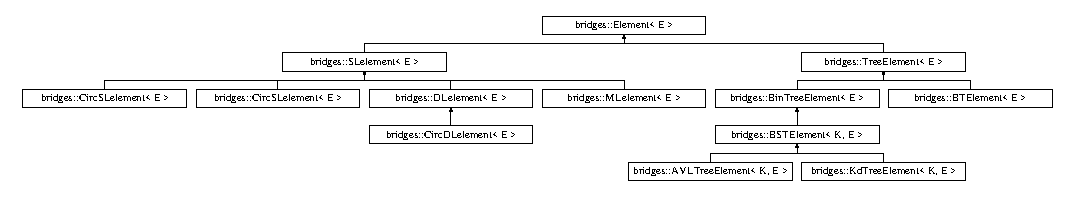
\includegraphics[height=2.641510cm]{classbridges_1_1_element}
\end{center}
\end{figure}
\subsection*{Public Member Functions}
\begin{DoxyCompactItemize}
\item 
\mbox{\hyperlink{classbridges_1_1_element_abc7131584142ea48faf3b7a8033d1fef}{Element}} (const E \&val=E(), const string \&lab=string())
\item 
\mbox{\hyperlink{classbridges_1_1_element_a6dc69b51f85f4e9914434b8c79126057}{Element}} (const \mbox{\hyperlink{classbridges_1_1_element}{Element}} \&e)
\item 
\mbox{\hyperlink{classbridges_1_1_element}{Element}} \& \mbox{\hyperlink{classbridges_1_1_element_a0f1b5a5688fe4db68f84969e93cea245}{operator=}} (const \mbox{\hyperlink{classbridges_1_1_element}{Element}} \&e)
\item 
virtual \mbox{\hyperlink{classbridges_1_1_element_a1dcdcd8948db683fc109687fe5d9c8e1}{$\sim$\+Element}} ()
\item 
\mbox{\hyperlink{classbridges_1_1_element_visualizer}{Element\+Visualizer}} $\ast$ \mbox{\hyperlink{classbridges_1_1_element_a358f350ae6e33d55c4ac9f9213d0c5bc}{get\+Visualizer}} ()
\item 
const \mbox{\hyperlink{classbridges_1_1_element_visualizer}{Element\+Visualizer}} $\ast$ \mbox{\hyperlink{classbridges_1_1_element_a27d023054130e17234ace34ba35e766e}{get\+Visualizer}} () const
\item 
\mbox{\hyperlink{classbridges_1_1_link_visualizer}{Link\+Visualizer}} $\ast$ \mbox{\hyperlink{classbridges_1_1_element_aa8dd91d04c22c697f7c500a18642282f}{get\+Link\+Visualizer}} (const \mbox{\hyperlink{classbridges_1_1_element}{Element}} $\ast$el)
\item 
\mbox{\hyperlink{classbridges_1_1_link_visualizer}{Link\+Visualizer}} $\ast$ \mbox{\hyperlink{classbridges_1_1_element_a202553f482b9a49057c8c87a368cc93a}{get\+Link\+Visualizer}} (const \mbox{\hyperlink{classbridges_1_1_element}{Element}} $\ast$el) const
\item 
string \mbox{\hyperlink{classbridges_1_1_element_a38df6d5f1e0203dfa85b073b6756194e}{get\+Label}} () const
\item 
void \mbox{\hyperlink{classbridges_1_1_element_a22313b74452175d07650168a701daa99}{set\+Label}} (const string \&lab)
\item 
E \mbox{\hyperlink{classbridges_1_1_element_a7df53b8b248020e9536bb951c725c7ba}{get\+Value}} () const
\item 
void \mbox{\hyperlink{classbridges_1_1_element_a737cb19281b6aa45a5a1dc9d592dad93}{set\+Value}} (const E \&val)
\item 
void \mbox{\hyperlink{classbridges_1_1_element_ae6f773c7222ff3a37c402e5e1f413c66}{print\+Links}} ()
\end{DoxyCompactItemize}
\subsection*{Protected Member Functions}
\begin{DoxyCompactItemize}
\item 
virtual const string \mbox{\hyperlink{classbridges_1_1_element_abfea1b7226b774be648e15f6b2c9daba}{get\+Element\+Representation}} () const
\end{DoxyCompactItemize}
\subsection*{Static Protected Member Functions}
\begin{DoxyCompactItemize}
\item 
static string \mbox{\hyperlink{classbridges_1_1_element_a0b905a076a71771a20ee4fb0ec858cfa}{remove\+Trailing\+Zeros}} (const double \&num)
\item 
static const string \mbox{\hyperlink{classbridges_1_1_element_ac6fa7b04e28a1e9b8d8f2d395dd6e2c1}{get\+Link\+Representation}} (const \mbox{\hyperlink{classbridges_1_1_link_visualizer}{Link\+Visualizer}} \&lv, const string \&src, const string \&dest)
\item 
static const string \mbox{\hyperlink{classbridges_1_1_element_a513b3409e4b689a390b0dcd50cc2d643}{get\+C\+S\+S\+Representation}} (const \mbox{\hyperlink{classbridges_1_1_color}{Color}} \&col)
\end{DoxyCompactItemize}
\subsection*{Protected Attributes}
\begin{DoxyCompactItemize}
\item 
unordered\+\_\+map$<$ \mbox{\hyperlink{classbridges_1_1_element}{Element}} $\ast$, \mbox{\hyperlink{classbridges_1_1_link_visualizer}{Link\+Visualizer}} $>$ \mbox{\hyperlink{classbridges_1_1_element_a6fb53728edc378f26238543b26238496}{links}}
\end{DoxyCompactItemize}
\subsection*{Friends}
\begin{DoxyCompactItemize}
\item 
{\footnotesize template$<$typename K , typename E1 , typename E2 $>$ }\\class \mbox{\hyperlink{classbridges_1_1_element_a65850138f0763fec43a76fb942f0eccc}{Graph\+Adj\+List}}
\item 
{\footnotesize template$<$typename K , typename E1 , typename E2 $>$ }\\class \mbox{\hyperlink{classbridges_1_1_element_a1935808473b7eb8ff54149c5436c3ac9}{Graph\+Adj\+Matrix}}
\item 
{\footnotesize template$<$typename K $>$ }\\class \mbox{\hyperlink{classbridges_1_1_element_ab1a595168ea1870ce436dfd2d8e69b6d}{Array}}
\end{DoxyCompactItemize}


\subsection{Detailed Description}
\subsubsection*{template$<$typename E$>$\newline
class bridges\+::\+Element$<$ E $>$}

This is the fundamental building block for all data structures in B\+R\+I\+D\+G\+ES. 

This is the Superclass \mbox{\hyperlink{classbridges_1_1_element}{Element}} with \mbox{\hyperlink{classbridges_1_1_s_lelement}{S\+Lelement}}, \mbox{\hyperlink{classbridges_1_1_d_lelement}{D\+Lelement}}, M\+L\+Element, Circ\+Sl\+Element, Circ\+Dl\+Element, \mbox{\hyperlink{classbridges_1_1_tree_element}{Tree\+Element}}, \mbox{\hyperlink{classbridges_1_1_a_v_l_tree_element}{A\+V\+L\+Tree\+Element}}, \mbox{\hyperlink{classbridges_1_1_b_s_t_element}{B\+S\+T\+Element}} subclasses.

Generic Parameters\+: E the application data type

The label field(string type) is used to label the visualization of the element.

\mbox{\hyperlink{classbridges_1_1_element}{Element}} holds a \mbox{\hyperlink{classbridges_1_1_link_visualizer}{Link\+Visualizer}} for each of its links and an \mbox{\hyperlink{classbridges_1_1_element_visualizer}{Element\+Visualizer}} for itself

\begin{DoxyAuthor}{Author}
Kalpathi Subramanian
\end{DoxyAuthor}
\begin{DoxyDate}{Date}
6/11/15, 11/27/16 
\end{DoxyDate}


\subsection{Constructor \& Destructor Documentation}
\mbox{\Hypertarget{classbridges_1_1_element_abc7131584142ea48faf3b7a8033d1fef}\label{classbridges_1_1_element_abc7131584142ea48faf3b7a8033d1fef}} 
\index{bridges\+::\+Element@{bridges\+::\+Element}!Element@{Element}}
\index{Element@{Element}!bridges\+::\+Element@{bridges\+::\+Element}}
\subsubsection{\texorpdfstring{Element()}{Element()}\hspace{0.1cm}{\footnotesize\ttfamily [1/2]}}
{\footnotesize\ttfamily template$<$typename E$>$ \\
\mbox{\hyperlink{classbridges_1_1_element}{bridges\+::\+Element}}$<$ E $>$\+::\mbox{\hyperlink{classbridges_1_1_element}{Element}} (\begin{DoxyParamCaption}\item[{const E \&}]{val = {\ttfamily E()},  }\item[{const string \&}]{lab = {\ttfamily string()} }\end{DoxyParamCaption})\hspace{0.3cm}{\ttfamily [inline]}}

Constructs an element with the provided value and label. The defaults will be used if not provided.


\begin{DoxyParams}{Parameters}
{\em val} & The data to hold \\
\hline
{\em lab} & The label to show \\
\hline
\end{DoxyParams}
\mbox{\Hypertarget{classbridges_1_1_element_a6dc69b51f85f4e9914434b8c79126057}\label{classbridges_1_1_element_a6dc69b51f85f4e9914434b8c79126057}} 
\index{bridges\+::\+Element@{bridges\+::\+Element}!Element@{Element}}
\index{Element@{Element}!bridges\+::\+Element@{bridges\+::\+Element}}
\subsubsection{\texorpdfstring{Element()}{Element()}\hspace{0.1cm}{\footnotesize\ttfamily [2/2]}}
{\footnotesize\ttfamily template$<$typename E$>$ \\
\mbox{\hyperlink{classbridges_1_1_element}{bridges\+::\+Element}}$<$ E $>$\+::\mbox{\hyperlink{classbridges_1_1_element}{Element}} (\begin{DoxyParamCaption}\item[{const \mbox{\hyperlink{classbridges_1_1_element}{Element}}$<$ E $>$ \&}]{e }\end{DoxyParamCaption})\hspace{0.3cm}{\ttfamily [inline]}}

\mbox{\Hypertarget{classbridges_1_1_element_a1dcdcd8948db683fc109687fe5d9c8e1}\label{classbridges_1_1_element_a1dcdcd8948db683fc109687fe5d9c8e1}} 
\index{bridges\+::\+Element@{bridges\+::\+Element}!````~Element@{$\sim$\+Element}}
\index{````~Element@{$\sim$\+Element}!bridges\+::\+Element@{bridges\+::\+Element}}
\subsubsection{\texorpdfstring{$\sim$\+Element()}{~Element()}}
{\footnotesize\ttfamily template$<$typename E$>$ \\
virtual \mbox{\hyperlink{classbridges_1_1_element}{bridges\+::\+Element}}$<$ E $>$\+::$\sim$\mbox{\hyperlink{classbridges_1_1_element}{Element}} (\begin{DoxyParamCaption}{ }\end{DoxyParamCaption})\hspace{0.3cm}{\ttfamily [inline]}, {\ttfamily [virtual]}}



\subsection{Member Function Documentation}
\mbox{\Hypertarget{classbridges_1_1_element_a513b3409e4b689a390b0dcd50cc2d643}\label{classbridges_1_1_element_a513b3409e4b689a390b0dcd50cc2d643}} 
\index{bridges\+::\+Element@{bridges\+::\+Element}!get\+C\+S\+S\+Representation@{get\+C\+S\+S\+Representation}}
\index{get\+C\+S\+S\+Representation@{get\+C\+S\+S\+Representation}!bridges\+::\+Element@{bridges\+::\+Element}}
\subsubsection{\texorpdfstring{get\+C\+S\+S\+Representation()}{getCSSRepresentation()}}
{\footnotesize\ttfamily template$<$typename E$>$ \\
static const string \mbox{\hyperlink{classbridges_1_1_element}{bridges\+::\+Element}}$<$ E $>$\+::get\+C\+S\+S\+Representation (\begin{DoxyParamCaption}\item[{const \mbox{\hyperlink{classbridges_1_1_color}{Color}} \&}]{col }\end{DoxyParamCaption})\hspace{0.3cm}{\ttfamily [inline]}, {\ttfamily [static]}, {\ttfamily [protected]}}

Gets the J\+S\+ON representation of this color


\begin{DoxyParams}{Parameters}
{\em col} & The \mbox{\hyperlink{classbridges_1_1_color}{Color}} \\
\hline
\end{DoxyParams}
\begin{DoxyReturn}{Returns}
Equivilant Legal C\+SS color representation 
\end{DoxyReturn}
\mbox{\Hypertarget{classbridges_1_1_element_abfea1b7226b774be648e15f6b2c9daba}\label{classbridges_1_1_element_abfea1b7226b774be648e15f6b2c9daba}} 
\index{bridges\+::\+Element@{bridges\+::\+Element}!get\+Element\+Representation@{get\+Element\+Representation}}
\index{get\+Element\+Representation@{get\+Element\+Representation}!bridges\+::\+Element@{bridges\+::\+Element}}
\subsubsection{\texorpdfstring{get\+Element\+Representation()}{getElementRepresentation()}}
{\footnotesize\ttfamily template$<$typename E$>$ \\
virtual const string \mbox{\hyperlink{classbridges_1_1_element}{bridges\+::\+Element}}$<$ E $>$\+::get\+Element\+Representation (\begin{DoxyParamCaption}{ }\end{DoxyParamCaption}) const\hspace{0.3cm}{\ttfamily [inline]}, {\ttfamily [protected]}, {\ttfamily [virtual]}}

\begin{DoxyReturn}{Returns}
The J\+S\+ON string of this element\textquotesingle{}s properties 
\end{DoxyReturn}


Reimplemented in \mbox{\hyperlink{classbridges_1_1_kd_tree_element_ad8aa2d89689f33691063fee9c601e2cb}{bridges\+::\+Kd\+Tree\+Element$<$ K, E $>$}}, and \mbox{\hyperlink{classbridges_1_1_b_s_t_element_a623d1495a0d27090dc3fc515d148f381}{bridges\+::\+B\+S\+T\+Element$<$ K, E $>$}}.

\mbox{\Hypertarget{classbridges_1_1_element_a38df6d5f1e0203dfa85b073b6756194e}\label{classbridges_1_1_element_a38df6d5f1e0203dfa85b073b6756194e}} 
\index{bridges\+::\+Element@{bridges\+::\+Element}!get\+Label@{get\+Label}}
\index{get\+Label@{get\+Label}!bridges\+::\+Element@{bridges\+::\+Element}}
\subsubsection{\texorpdfstring{get\+Label()}{getLabel()}}
{\footnotesize\ttfamily template$<$typename E$>$ \\
string \mbox{\hyperlink{classbridges_1_1_element}{bridges\+::\+Element}}$<$ E $>$\+::get\+Label (\begin{DoxyParamCaption}{ }\end{DoxyParamCaption}) const\hspace{0.3cm}{\ttfamily [inline]}}

\begin{DoxyReturn}{Returns}
The label of the element 
\end{DoxyReturn}
\mbox{\Hypertarget{classbridges_1_1_element_ac6fa7b04e28a1e9b8d8f2d395dd6e2c1}\label{classbridges_1_1_element_ac6fa7b04e28a1e9b8d8f2d395dd6e2c1}} 
\index{bridges\+::\+Element@{bridges\+::\+Element}!get\+Link\+Representation@{get\+Link\+Representation}}
\index{get\+Link\+Representation@{get\+Link\+Representation}!bridges\+::\+Element@{bridges\+::\+Element}}
\subsubsection{\texorpdfstring{get\+Link\+Representation()}{getLinkRepresentation()}}
{\footnotesize\ttfamily template$<$typename E$>$ \\
static const string \mbox{\hyperlink{classbridges_1_1_element}{bridges\+::\+Element}}$<$ E $>$\+::get\+Link\+Representation (\begin{DoxyParamCaption}\item[{const \mbox{\hyperlink{classbridges_1_1_link_visualizer}{Link\+Visualizer}} \&}]{lv,  }\item[{const string \&}]{src,  }\item[{const string \&}]{dest }\end{DoxyParamCaption})\hspace{0.3cm}{\ttfamily [inline]}, {\ttfamily [static]}, {\ttfamily [protected]}}

Gets the J\+S\+ON representation of this link visualizer using the supplied source and destination strings


\begin{DoxyParams}{Parameters}
{\em lv} & The \mbox{\hyperlink{classbridges_1_1_link_visualizer}{Link\+Visualizer}} \\
\hline
{\em src} & The source vertex \\
\hline
{\em dest} & The destination vertex \\
\hline
\end{DoxyParams}
\begin{DoxyReturn}{Returns}
The J\+S\+ON of this link visualizer 
\end{DoxyReturn}
\mbox{\Hypertarget{classbridges_1_1_element_aa8dd91d04c22c697f7c500a18642282f}\label{classbridges_1_1_element_aa8dd91d04c22c697f7c500a18642282f}} 
\index{bridges\+::\+Element@{bridges\+::\+Element}!get\+Link\+Visualizer@{get\+Link\+Visualizer}}
\index{get\+Link\+Visualizer@{get\+Link\+Visualizer}!bridges\+::\+Element@{bridges\+::\+Element}}
\subsubsection{\texorpdfstring{get\+Link\+Visualizer()}{getLinkVisualizer()}\hspace{0.1cm}{\footnotesize\ttfamily [1/2]}}
{\footnotesize\ttfamily template$<$typename E$>$ \\
\mbox{\hyperlink{classbridges_1_1_link_visualizer}{Link\+Visualizer}}$\ast$ \mbox{\hyperlink{classbridges_1_1_element}{bridges\+::\+Element}}$<$ E $>$\+::get\+Link\+Visualizer (\begin{DoxyParamCaption}\item[{const \mbox{\hyperlink{classbridges_1_1_element}{Element}}$<$ E $>$ $\ast$}]{el }\end{DoxyParamCaption})\hspace{0.3cm}{\ttfamily [inline]}}

Returns the \mbox{\hyperlink{classbridges_1_1_link_visualizer}{Link\+Visualizer}} to element \char`\"{}el\char`\"{} or N\+U\+LL if no link exists


\begin{DoxyParams}{Parameters}
{\em el} & The terminating element of the link\\
\hline
\end{DoxyParams}
\begin{DoxyReturn}{Returns}
The \mbox{\hyperlink{classbridges_1_1_link_visualizer}{Link\+Visualizer}} 
\end{DoxyReturn}
\mbox{\Hypertarget{classbridges_1_1_element_a202553f482b9a49057c8c87a368cc93a}\label{classbridges_1_1_element_a202553f482b9a49057c8c87a368cc93a}} 
\index{bridges\+::\+Element@{bridges\+::\+Element}!get\+Link\+Visualizer@{get\+Link\+Visualizer}}
\index{get\+Link\+Visualizer@{get\+Link\+Visualizer}!bridges\+::\+Element@{bridges\+::\+Element}}
\subsubsection{\texorpdfstring{get\+Link\+Visualizer()}{getLinkVisualizer()}\hspace{0.1cm}{\footnotesize\ttfamily [2/2]}}
{\footnotesize\ttfamily template$<$typename E$>$ \\
\mbox{\hyperlink{classbridges_1_1_link_visualizer}{Link\+Visualizer}}$\ast$ \mbox{\hyperlink{classbridges_1_1_element}{bridges\+::\+Element}}$<$ E $>$\+::get\+Link\+Visualizer (\begin{DoxyParamCaption}\item[{const \mbox{\hyperlink{classbridges_1_1_element}{Element}}$<$ E $>$ $\ast$}]{el }\end{DoxyParamCaption}) const\hspace{0.3cm}{\ttfamily [inline]}}

Constant version


\begin{DoxyParams}{Parameters}
{\em el} & The terminating element of the link \\
\hline
\end{DoxyParams}
\begin{DoxyReturn}{Returns}
The \mbox{\hyperlink{classbridges_1_1_link_visualizer}{Link\+Visualizer}} 
\end{DoxyReturn}
\mbox{\Hypertarget{classbridges_1_1_element_a7df53b8b248020e9536bb951c725c7ba}\label{classbridges_1_1_element_a7df53b8b248020e9536bb951c725c7ba}} 
\index{bridges\+::\+Element@{bridges\+::\+Element}!get\+Value@{get\+Value}}
\index{get\+Value@{get\+Value}!bridges\+::\+Element@{bridges\+::\+Element}}
\subsubsection{\texorpdfstring{get\+Value()}{getValue()}}
{\footnotesize\ttfamily template$<$typename E$>$ \\
E \mbox{\hyperlink{classbridges_1_1_element}{bridges\+::\+Element}}$<$ E $>$\+::get\+Value (\begin{DoxyParamCaption}{ }\end{DoxyParamCaption}) const\hspace{0.3cm}{\ttfamily [inline]}}

\begin{DoxyReturn}{Returns}
The value of the element 
\end{DoxyReturn}
\mbox{\Hypertarget{classbridges_1_1_element_a358f350ae6e33d55c4ac9f9213d0c5bc}\label{classbridges_1_1_element_a358f350ae6e33d55c4ac9f9213d0c5bc}} 
\index{bridges\+::\+Element@{bridges\+::\+Element}!get\+Visualizer@{get\+Visualizer}}
\index{get\+Visualizer@{get\+Visualizer}!bridges\+::\+Element@{bridges\+::\+Element}}
\subsubsection{\texorpdfstring{get\+Visualizer()}{getVisualizer()}\hspace{0.1cm}{\footnotesize\ttfamily [1/2]}}
{\footnotesize\ttfamily template$<$typename E$>$ \\
\mbox{\hyperlink{classbridges_1_1_element_visualizer}{Element\+Visualizer}}$\ast$ \mbox{\hyperlink{classbridges_1_1_element}{bridges\+::\+Element}}$<$ E $>$\+::get\+Visualizer (\begin{DoxyParamCaption}{ }\end{DoxyParamCaption})\hspace{0.3cm}{\ttfamily [inline]}}

\begin{DoxyReturn}{Returns}
The \mbox{\hyperlink{classbridges_1_1_element_visualizer}{Element\+Visualizer}} of this element 
\end{DoxyReturn}
\mbox{\Hypertarget{classbridges_1_1_element_a27d023054130e17234ace34ba35e766e}\label{classbridges_1_1_element_a27d023054130e17234ace34ba35e766e}} 
\index{bridges\+::\+Element@{bridges\+::\+Element}!get\+Visualizer@{get\+Visualizer}}
\index{get\+Visualizer@{get\+Visualizer}!bridges\+::\+Element@{bridges\+::\+Element}}
\subsubsection{\texorpdfstring{get\+Visualizer()}{getVisualizer()}\hspace{0.1cm}{\footnotesize\ttfamily [2/2]}}
{\footnotesize\ttfamily template$<$typename E$>$ \\
const \mbox{\hyperlink{classbridges_1_1_element_visualizer}{Element\+Visualizer}}$\ast$ \mbox{\hyperlink{classbridges_1_1_element}{bridges\+::\+Element}}$<$ E $>$\+::get\+Visualizer (\begin{DoxyParamCaption}{ }\end{DoxyParamCaption}) const\hspace{0.3cm}{\ttfamily [inline]}}

Constant version

\begin{DoxyReturn}{Returns}
The \mbox{\hyperlink{classbridges_1_1_element_visualizer}{Element\+Visualizer}} of this element 
\end{DoxyReturn}
\mbox{\Hypertarget{classbridges_1_1_element_a0f1b5a5688fe4db68f84969e93cea245}\label{classbridges_1_1_element_a0f1b5a5688fe4db68f84969e93cea245}} 
\index{bridges\+::\+Element@{bridges\+::\+Element}!operator=@{operator=}}
\index{operator=@{operator=}!bridges\+::\+Element@{bridges\+::\+Element}}
\subsubsection{\texorpdfstring{operator=()}{operator=()}}
{\footnotesize\ttfamily template$<$typename E$>$ \\
\mbox{\hyperlink{classbridges_1_1_element}{Element}}\& \mbox{\hyperlink{classbridges_1_1_element}{bridges\+::\+Element}}$<$ E $>$\+::operator= (\begin{DoxyParamCaption}\item[{const \mbox{\hyperlink{classbridges_1_1_element}{Element}}$<$ E $>$ \&}]{e }\end{DoxyParamCaption})\hspace{0.3cm}{\ttfamily [inline]}}

\mbox{\Hypertarget{classbridges_1_1_element_ae6f773c7222ff3a37c402e5e1f413c66}\label{classbridges_1_1_element_ae6f773c7222ff3a37c402e5e1f413c66}} 
\index{bridges\+::\+Element@{bridges\+::\+Element}!print\+Links@{print\+Links}}
\index{print\+Links@{print\+Links}!bridges\+::\+Element@{bridges\+::\+Element}}
\subsubsection{\texorpdfstring{print\+Links()}{printLinks()}}
{\footnotesize\ttfamily template$<$typename E$>$ \\
void \mbox{\hyperlink{classbridges_1_1_element}{bridges\+::\+Element}}$<$ E $>$\+::print\+Links (\begin{DoxyParamCaption}{ }\end{DoxyParamCaption})\hspace{0.3cm}{\ttfamily [inline]}}

\mbox{\Hypertarget{classbridges_1_1_element_a0b905a076a71771a20ee4fb0ec858cfa}\label{classbridges_1_1_element_a0b905a076a71771a20ee4fb0ec858cfa}} 
\index{bridges\+::\+Element@{bridges\+::\+Element}!remove\+Trailing\+Zeros@{remove\+Trailing\+Zeros}}
\index{remove\+Trailing\+Zeros@{remove\+Trailing\+Zeros}!bridges\+::\+Element@{bridges\+::\+Element}}
\subsubsection{\texorpdfstring{remove\+Trailing\+Zeros()}{removeTrailingZeros()}}
{\footnotesize\ttfamily template$<$typename E$>$ \\
static string \mbox{\hyperlink{classbridges_1_1_element}{bridges\+::\+Element}}$<$ E $>$\+::remove\+Trailing\+Zeros (\begin{DoxyParamCaption}\item[{const double \&}]{num }\end{DoxyParamCaption})\hspace{0.3cm}{\ttfamily [inline]}, {\ttfamily [static]}, {\ttfamily [protected]}}

\begin{DoxyReturn}{Returns}
to\+\_\+string of \char`\"{}num\char`\"{} without unnessasary trailing 0s 
\end{DoxyReturn}
\mbox{\Hypertarget{classbridges_1_1_element_a22313b74452175d07650168a701daa99}\label{classbridges_1_1_element_a22313b74452175d07650168a701daa99}} 
\index{bridges\+::\+Element@{bridges\+::\+Element}!set\+Label@{set\+Label}}
\index{set\+Label@{set\+Label}!bridges\+::\+Element@{bridges\+::\+Element}}
\subsubsection{\texorpdfstring{set\+Label()}{setLabel()}}
{\footnotesize\ttfamily template$<$typename E$>$ \\
void \mbox{\hyperlink{classbridges_1_1_element}{bridges\+::\+Element}}$<$ E $>$\+::set\+Label (\begin{DoxyParamCaption}\item[{const string \&}]{lab }\end{DoxyParamCaption})\hspace{0.3cm}{\ttfamily [inline]}}

Sets label to \char`\"{}lab\char`\"{}


\begin{DoxyParams}{Parameters}
{\em lab} & The label of the element \\
\hline
\end{DoxyParams}
\mbox{\Hypertarget{classbridges_1_1_element_a737cb19281b6aa45a5a1dc9d592dad93}\label{classbridges_1_1_element_a737cb19281b6aa45a5a1dc9d592dad93}} 
\index{bridges\+::\+Element@{bridges\+::\+Element}!set\+Value@{set\+Value}}
\index{set\+Value@{set\+Value}!bridges\+::\+Element@{bridges\+::\+Element}}
\subsubsection{\texorpdfstring{set\+Value()}{setValue()}}
{\footnotesize\ttfamily template$<$typename E$>$ \\
void \mbox{\hyperlink{classbridges_1_1_element}{bridges\+::\+Element}}$<$ E $>$\+::set\+Value (\begin{DoxyParamCaption}\item[{const E \&}]{val }\end{DoxyParamCaption})\hspace{0.3cm}{\ttfamily [inline]}}

Sets value to \char`\"{}val\char`\"{}


\begin{DoxyParams}{Parameters}
{\em val} & The value of the element \\
\hline
\end{DoxyParams}


\subsection{Friends And Related Function Documentation}
\mbox{\Hypertarget{classbridges_1_1_element_ab1a595168ea1870ce436dfd2d8e69b6d}\label{classbridges_1_1_element_ab1a595168ea1870ce436dfd2d8e69b6d}} 
\index{bridges\+::\+Element@{bridges\+::\+Element}!Array@{Array}}
\index{Array@{Array}!bridges\+::\+Element@{bridges\+::\+Element}}
\subsubsection{\texorpdfstring{Array}{Array}}
{\footnotesize\ttfamily template$<$typename E$>$ \\
template$<$typename K $>$ \\
friend class \mbox{\hyperlink{classbridges_1_1_array}{Array}}\hspace{0.3cm}{\ttfamily [friend]}}

\mbox{\Hypertarget{classbridges_1_1_element_a65850138f0763fec43a76fb942f0eccc}\label{classbridges_1_1_element_a65850138f0763fec43a76fb942f0eccc}} 
\index{bridges\+::\+Element@{bridges\+::\+Element}!Graph\+Adj\+List@{Graph\+Adj\+List}}
\index{Graph\+Adj\+List@{Graph\+Adj\+List}!bridges\+::\+Element@{bridges\+::\+Element}}
\subsubsection{\texorpdfstring{Graph\+Adj\+List}{GraphAdjList}}
{\footnotesize\ttfamily template$<$typename E$>$ \\
template$<$typename K , typename E1 , typename E2 $>$ \\
friend class \mbox{\hyperlink{classbridges_1_1_graph_adj_list}{Graph\+Adj\+List}}\hspace{0.3cm}{\ttfamily [friend]}}

\mbox{\Hypertarget{classbridges_1_1_element_a1935808473b7eb8ff54149c5436c3ac9}\label{classbridges_1_1_element_a1935808473b7eb8ff54149c5436c3ac9}} 
\index{bridges\+::\+Element@{bridges\+::\+Element}!Graph\+Adj\+Matrix@{Graph\+Adj\+Matrix}}
\index{Graph\+Adj\+Matrix@{Graph\+Adj\+Matrix}!bridges\+::\+Element@{bridges\+::\+Element}}
\subsubsection{\texorpdfstring{Graph\+Adj\+Matrix}{GraphAdjMatrix}}
{\footnotesize\ttfamily template$<$typename E$>$ \\
template$<$typename K , typename E1 , typename E2 $>$ \\
friend class \mbox{\hyperlink{classbridges_1_1_graph_adj_matrix}{Graph\+Adj\+Matrix}}\hspace{0.3cm}{\ttfamily [friend]}}



\subsection{Member Data Documentation}
\mbox{\Hypertarget{classbridges_1_1_element_a6fb53728edc378f26238543b26238496}\label{classbridges_1_1_element_a6fb53728edc378f26238543b26238496}} 
\index{bridges\+::\+Element@{bridges\+::\+Element}!links@{links}}
\index{links@{links}!bridges\+::\+Element@{bridges\+::\+Element}}
\subsubsection{\texorpdfstring{links}{links}}
{\footnotesize\ttfamily template$<$typename E$>$ \\
unordered\+\_\+map$<$\mbox{\hyperlink{classbridges_1_1_element}{Element}}$\ast$, \mbox{\hyperlink{classbridges_1_1_link_visualizer}{Link\+Visualizer}}$>$ \mbox{\hyperlink{classbridges_1_1_element}{bridges\+::\+Element}}$<$ E $>$\+::links\hspace{0.3cm}{\ttfamily [protected]}}



The documentation for this class was generated from the following file\+:\begin{DoxyCompactItemize}
\item 
/\+Users/kalpathi/gr/bridges/client/cxx/bridges17/src/\mbox{\hyperlink{_element_8h}{Element.\+h}}\end{DoxyCompactItemize}

\hypertarget{classbridges_1_1_element_array}{}\section{bridges\+:\+:Element\+Array$<$ E, X, Y, Z $>$ Class Template Reference}
\label{classbridges_1_1_element_array}\index{bridges\+::\+Element\+Array$<$ E, X, Y, Z $>$@{bridges\+::\+Element\+Array$<$ E, X, Y, Z $>$}}


Currently unused class, ignore.  




{\ttfamily \#include $<$Element\+Array.\+h$>$}

Inheritance diagram for bridges\+:\+:Element\+Array$<$ E, X, Y, Z $>$\+:\begin{figure}[H]
\begin{center}
\leavevmode
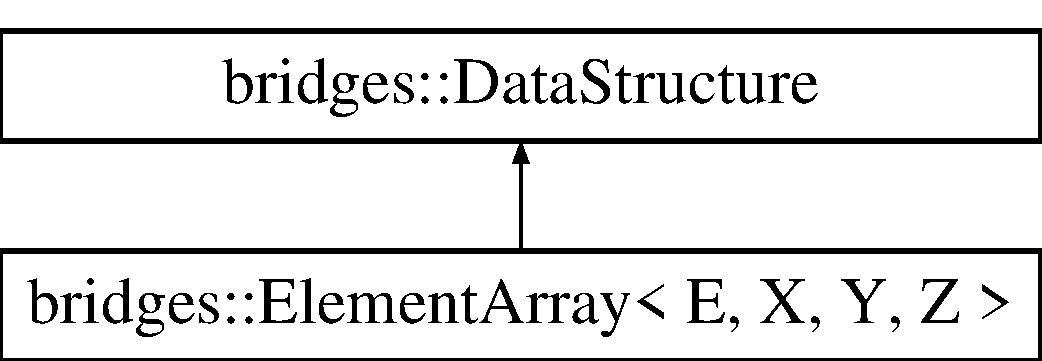
\includegraphics[height=2.000000cm]{classbridges_1_1_element_array}
\end{center}
\end{figure}
\subsection*{Public Member Functions}
\begin{DoxyCompactItemize}
\item 
\hyperlink{classbridges_1_1_element_array_aef0cfb2b7b35cd5b368e4c3987e41768}{Element\+Array} ()
\item 
\hyperlink{classbridges_1_1_element}{Element}$<$ E $>$ $\ast$ \hyperlink{classbridges_1_1_element_array_a45bac55f6f64a90eb61fd3faaf1aaffe}{get\+Value} (size\+\_\+t x, size\+\_\+t y=0, size\+\_\+t z=0)
\item 
const \hyperlink{classbridges_1_1_element}{Element}$<$ E $>$ $\ast$ \hyperlink{classbridges_1_1_element_array_ab10a4e60f7d17e9112f87db672869a41}{get\+Value} (size\+\_\+t x, size\+\_\+t y=0, size\+\_\+t z=0) const 
\item 
void \hyperlink{classbridges_1_1_element_array_a202def849cd345d8b56ebcb31f332d25}{set\+Value} (\hyperlink{classbridges_1_1_element}{Element}$<$ E $>$ $\ast$el, size\+\_\+t x, size\+\_\+t y=0, size\+\_\+t z=0)
\item 
virtual const string \hyperlink{classbridges_1_1_element_array_a19e80a81e4d27f13e4a2091f371a7e18}{get\+D\+Stype} () const  override
\end{DoxyCompactItemize}


\subsection{Detailed Description}
\subsubsection*{template$<$typename E, size\+\_\+t X, size\+\_\+t Y = 1, size\+\_\+t Z = 1$>$class bridges\+::\+Element\+Array$<$ E, X, Y, Z $>$}

Currently unused class, ignore. 

\subsection{Constructor \& Destructor Documentation}
\hypertarget{classbridges_1_1_element_array_aef0cfb2b7b35cd5b368e4c3987e41768}{}\index{bridges\+::\+Element\+Array@{bridges\+::\+Element\+Array}!Element\+Array@{Element\+Array}}
\index{Element\+Array@{Element\+Array}!bridges\+::\+Element\+Array@{bridges\+::\+Element\+Array}}
\subsubsection[{Element\+Array()}]{\setlength{\rightskip}{0pt plus 5cm}template$<$typename E , size\+\_\+t X, size\+\_\+t Y = 1, size\+\_\+t Z = 1$>$ {\bf bridges\+::\+Element\+Array}$<$ E, X, Y, Z $>$\+::{\bf Element\+Array} (
\begin{DoxyParamCaption}
{}
\end{DoxyParamCaption}
)\hspace{0.3cm}{\ttfamily [inline]}}\label{classbridges_1_1_element_array_aef0cfb2b7b35cd5b368e4c3987e41768}


\subsection{Member Function Documentation}
\hypertarget{classbridges_1_1_element_array_a19e80a81e4d27f13e4a2091f371a7e18}{}\index{bridges\+::\+Element\+Array@{bridges\+::\+Element\+Array}!get\+D\+Stype@{get\+D\+Stype}}
\index{get\+D\+Stype@{get\+D\+Stype}!bridges\+::\+Element\+Array@{bridges\+::\+Element\+Array}}
\subsubsection[{get\+D\+Stype() const  override}]{\setlength{\rightskip}{0pt plus 5cm}template$<$typename E , size\+\_\+t X, size\+\_\+t Y = 1, size\+\_\+t Z = 1$>$ virtual const string {\bf bridges\+::\+Element\+Array}$<$ E, X, Y, Z $>$\+::get\+D\+Stype (
\begin{DoxyParamCaption}
{}
\end{DoxyParamCaption}
) const\hspace{0.3cm}{\ttfamily [inline]}, {\ttfamily [override]}, {\ttfamily [virtual]}}\label{classbridges_1_1_element_array_a19e80a81e4d27f13e4a2091f371a7e18}
\begin{DoxyReturn}{Returns}
The string representation of this data structure type 
\end{DoxyReturn}


Implements \hyperlink{classbridges_1_1_data_structure_ab6973cdb2a22b7e664b895f1f9c8ad54}{bridges\+::\+Data\+Structure}.

\hypertarget{classbridges_1_1_element_array_a45bac55f6f64a90eb61fd3faaf1aaffe}{}\index{bridges\+::\+Element\+Array@{bridges\+::\+Element\+Array}!get\+Value@{get\+Value}}
\index{get\+Value@{get\+Value}!bridges\+::\+Element\+Array@{bridges\+::\+Element\+Array}}
\subsubsection[{get\+Value(size\+\_\+t x, size\+\_\+t y=0, size\+\_\+t z=0)}]{\setlength{\rightskip}{0pt plus 5cm}template$<$typename E , size\+\_\+t X, size\+\_\+t Y = 1, size\+\_\+t Z = 1$>$ {\bf Element}$<$E$>$$\ast$ {\bf bridges\+::\+Element\+Array}$<$ E, X, Y, Z $>$\+::get\+Value (
\begin{DoxyParamCaption}
\item[{size\+\_\+t}]{x, }
\item[{size\+\_\+t}]{y = {\ttfamily 0}, }
\item[{size\+\_\+t}]{z = {\ttfamily 0}}
\end{DoxyParamCaption}
)\hspace{0.3cm}{\ttfamily [inline]}}\label{classbridges_1_1_element_array_a45bac55f6f64a90eb61fd3faaf1aaffe}
\hypertarget{classbridges_1_1_element_array_ab10a4e60f7d17e9112f87db672869a41}{}\index{bridges\+::\+Element\+Array@{bridges\+::\+Element\+Array}!get\+Value@{get\+Value}}
\index{get\+Value@{get\+Value}!bridges\+::\+Element\+Array@{bridges\+::\+Element\+Array}}
\subsubsection[{get\+Value(size\+\_\+t x, size\+\_\+t y=0, size\+\_\+t z=0) const }]{\setlength{\rightskip}{0pt plus 5cm}template$<$typename E , size\+\_\+t X, size\+\_\+t Y = 1, size\+\_\+t Z = 1$>$ const {\bf Element}$<$E$>$$\ast$ {\bf bridges\+::\+Element\+Array}$<$ E, X, Y, Z $>$\+::get\+Value (
\begin{DoxyParamCaption}
\item[{size\+\_\+t}]{x, }
\item[{size\+\_\+t}]{y = {\ttfamily 0}, }
\item[{size\+\_\+t}]{z = {\ttfamily 0}}
\end{DoxyParamCaption}
) const\hspace{0.3cm}{\ttfamily [inline]}}\label{classbridges_1_1_element_array_ab10a4e60f7d17e9112f87db672869a41}
\hypertarget{classbridges_1_1_element_array_a202def849cd345d8b56ebcb31f332d25}{}\index{bridges\+::\+Element\+Array@{bridges\+::\+Element\+Array}!set\+Value@{set\+Value}}
\index{set\+Value@{set\+Value}!bridges\+::\+Element\+Array@{bridges\+::\+Element\+Array}}
\subsubsection[{set\+Value(\+Element$<$ E $>$ $\ast$el, size\+\_\+t x, size\+\_\+t y=0, size\+\_\+t z=0)}]{\setlength{\rightskip}{0pt plus 5cm}template$<$typename E , size\+\_\+t X, size\+\_\+t Y = 1, size\+\_\+t Z = 1$>$ void {\bf bridges\+::\+Element\+Array}$<$ E, X, Y, Z $>$\+::set\+Value (
\begin{DoxyParamCaption}
\item[{{\bf Element}$<$ E $>$ $\ast$}]{el, }
\item[{size\+\_\+t}]{x, }
\item[{size\+\_\+t}]{y = {\ttfamily 0}, }
\item[{size\+\_\+t}]{z = {\ttfamily 0}}
\end{DoxyParamCaption}
)\hspace{0.3cm}{\ttfamily [inline]}}\label{classbridges_1_1_element_array_a202def849cd345d8b56ebcb31f332d25}


The documentation for this class was generated from the following file\+:\begin{DoxyCompactItemize}
\item 
/\+Users/krs/gr/bridges/client/cxx/src/\hyperlink{_element_array_8h}{Element\+Array.\+h}\end{DoxyCompactItemize}

\hypertarget{classbridges_1_1_element_visualizer}{}\section{bridges\+:\+:Element\+Visualizer Class Reference}
\label{classbridges_1_1_element_visualizer}\index{bridges\+::\+Element\+Visualizer@{bridges\+::\+Element\+Visualizer}}


This class maintains the visual properties of the a \hyperlink{namespacebridges_1_1_bridges}{Bridges} element.  




{\ttfamily \#include $<$Element\+Visualizer.\+h$>$}

\subsection*{Public Member Functions}
\begin{DoxyCompactItemize}
\item 
\hyperlink{classbridges_1_1_element_visualizer_af792c8b0aaa76d07f5806df83f27ccb6}{Element\+Visualizer} (const \hyperlink{classbridges_1_1_color}{Color} \&hue=\hyperlink{classbridges_1_1_element_visualizer_ade224640b18e3f6eed42098ea0ad5b3a}{D\+E\+F\+A\+U\+L\+T\+\_\+\+C\+O\+L\+O\+R}, const double \&sz=\hyperlink{classbridges_1_1_element_visualizer_a81cc788d6149d5d582099cbc35e18c5a}{D\+E\+F\+A\+U\+L\+T\+\_\+\+S\+I\+Z\+E}, const \hyperlink{namespacebridges_a1b4050586bd708782ae0d4f3b06b9579}{Shape} \&shp=\hyperlink{classbridges_1_1_element_visualizer_a2800a212357180e4941a818b958aabd9}{D\+E\+F\+A\+U\+L\+T\+\_\+\+S\+H\+A\+P\+E})
\item 
void \hyperlink{classbridges_1_1_element_visualizer_a6fc924e754008992b310a89d8d88fce9}{set\+Size} (const double \&sz)
\item 
double \hyperlink{classbridges_1_1_element_visualizer_aae6ce4807e470d0bda96cf6753e81669}{get\+Size} () const 
\item 
void \hyperlink{classbridges_1_1_element_visualizer_af14723066e52c159eebfb804d65dd825}{set\+Color} (const \hyperlink{classbridges_1_1_color}{Color} \&col)
\item 
\hyperlink{classbridges_1_1_color}{Color} \hyperlink{classbridges_1_1_element_visualizer_a93012c4fb2d8a67128b5c83cc8e5c190}{get\+Color} () const 
\item 
void \hyperlink{classbridges_1_1_element_visualizer_a8f77db4a2774021aec4ab8ea18e50fc9}{set\+Opacity} (double opacity)
\item 
double \hyperlink{classbridges_1_1_element_visualizer_ae806977ebc8ff1c5bce81c90b31902b5}{get\+Opacity} ()
\item 
void \hyperlink{classbridges_1_1_element_visualizer_af81cc20423f2fedffa81fb7c473a1179}{set\+Shape} (const \hyperlink{namespacebridges_a1b4050586bd708782ae0d4f3b06b9579}{Shape} \&shp)
\item 
\hyperlink{namespacebridges_a1b4050586bd708782ae0d4f3b06b9579}{Shape} \hyperlink{classbridges_1_1_element_visualizer_a3e1bb5ba7ae2e5a23fbb75c7b09d350c}{get\+Shape} () const 
\item 
void \hyperlink{classbridges_1_1_element_visualizer_ad06f2fd509f6b3474feeb4fa1fef38d5}{set\+Location} (const double \&loc\+X, const double \&loc\+Y)
\item 
double \hyperlink{classbridges_1_1_element_visualizer_a660dfe007963b4e9314a5da07f776e78}{get\+Location\+X} () const 
\item 
double \hyperlink{classbridges_1_1_element_visualizer_acbd58b69a2b8e44735e4c87783710439}{get\+Location\+Y} () const 
\end{DoxyCompactItemize}
\subsection*{Static Public Attributes}
\begin{DoxyCompactItemize}
\item 
static const \hyperlink{classbridges_1_1_color}{Color} \hyperlink{classbridges_1_1_element_visualizer_ade224640b18e3f6eed42098ea0ad5b3a}{D\+E\+F\+A\+U\+L\+T\+\_\+\+C\+O\+L\+O\+R}
\item 
static constexpr \hyperlink{namespacebridges_a1b4050586bd708782ae0d4f3b06b9579}{Shape} \hyperlink{classbridges_1_1_element_visualizer_a2800a212357180e4941a818b958aabd9}{D\+E\+F\+A\+U\+L\+T\+\_\+\+S\+H\+A\+P\+E} = \hyperlink{namespacebridges_a1b4050586bd708782ae0d4f3b06b9579aa968bf0f7aeccbae1a40751345bf2e64}{C\+I\+R\+C\+L\+E}
\item 
static constexpr double \hyperlink{classbridges_1_1_element_visualizer_a81cc788d6149d5d582099cbc35e18c5a}{D\+E\+F\+A\+U\+L\+T\+\_\+\+S\+I\+Z\+E} = 10
\end{DoxyCompactItemize}


\subsection{Detailed Description}
This class maintains the visual properties of the a \hyperlink{namespacebridges_1_1_bridges}{Bridges} element. 

This class is used to store the visualization elements for \hyperlink{namespacebridges_1_1_bridges}{Bridges} Visualiztions, including the color, shape, and size of the node. Defaults of green, circle, and 10.\+0 respectively.

Size values must range from \mbox{[}10.\+0,50.\+0\mbox{]}. B\+R\+I\+D\+G\+E\+S supports the following shapes\+: \char`\"{}circle\char`\"{}, \char`\"{}square\char`\"{}, \char`\"{}diamond\char`\"{}, \char`\"{}cross\char`\"{}, \char`\"{}triangle-\/down\char`\"{}, \char`\"{}triangle-\/up\char`\"{}

Objects of this class are stored as properties of all \hyperlink{classbridges_1_1_element}{Element} subclasses.

\begin{DoxyAuthor}{Author}
Kalpathi Subramanian 
\end{DoxyAuthor}
\begin{DoxyDate}{Date}
6/11/15 
\end{DoxyDate}


\subsection{Constructor \& Destructor Documentation}
\hypertarget{classbridges_1_1_element_visualizer_af792c8b0aaa76d07f5806df83f27ccb6}{}\index{bridges\+::\+Element\+Visualizer@{bridges\+::\+Element\+Visualizer}!Element\+Visualizer@{Element\+Visualizer}}
\index{Element\+Visualizer@{Element\+Visualizer}!bridges\+::\+Element\+Visualizer@{bridges\+::\+Element\+Visualizer}}
\subsubsection[{Element\+Visualizer(const Color \&hue=\+D\+E\+F\+A\+U\+L\+T\+\_\+\+C\+O\+L\+O\+R, const double \&sz=\+D\+E\+F\+A\+U\+L\+T\+\_\+\+S\+I\+Z\+E, const Shape \&shp=\+D\+E\+F\+A\+U\+L\+T\+\_\+\+S\+H\+A\+P\+E)}]{\setlength{\rightskip}{0pt plus 5cm}bridges\+::\+Element\+Visualizer\+::\+Element\+Visualizer (
\begin{DoxyParamCaption}
\item[{const {\bf Color} \&}]{hue = {\ttfamily {\bf D\+E\+F\+A\+U\+L\+T\+\_\+\+C\+O\+L\+O\+R}}, }
\item[{const double \&}]{sz = {\ttfamily {\bf D\+E\+F\+A\+U\+L\+T\+\_\+\+S\+I\+Z\+E}}, }
\item[{const {\bf Shape} \&}]{shp = {\ttfamily {\bf D\+E\+F\+A\+U\+L\+T\+\_\+\+S\+H\+A\+P\+E}}}
\end{DoxyParamCaption}
)\hspace{0.3cm}{\ttfamily [inline]}}\label{classbridges_1_1_element_visualizer_af792c8b0aaa76d07f5806df83f27ccb6}
Constructs an element with the provided \hyperlink{classbridges_1_1_color}{Color}, Size, and Shape. The defaults will be used if not provided.


\begin{DoxyParams}{Parameters}
{\em hue} & The \hyperlink{classbridges_1_1_color}{Color} for display \\
\hline
{\em sz} & The Size for display \\
\hline
{\em shp} & The Shape for display \\
\hline
\end{DoxyParams}


\subsection{Member Function Documentation}
\hypertarget{classbridges_1_1_element_visualizer_a93012c4fb2d8a67128b5c83cc8e5c190}{}\index{bridges\+::\+Element\+Visualizer@{bridges\+::\+Element\+Visualizer}!get\+Color@{get\+Color}}
\index{get\+Color@{get\+Color}!bridges\+::\+Element\+Visualizer@{bridges\+::\+Element\+Visualizer}}
\subsubsection[{get\+Color() const }]{\setlength{\rightskip}{0pt plus 5cm}{\bf Color} bridges\+::\+Element\+Visualizer\+::get\+Color (
\begin{DoxyParamCaption}
{}
\end{DoxyParamCaption}
) const\hspace{0.3cm}{\ttfamily [inline]}}\label{classbridges_1_1_element_visualizer_a93012c4fb2d8a67128b5c83cc8e5c190}
\begin{DoxyReturn}{Returns}
The color of the element 
\end{DoxyReturn}
\hypertarget{classbridges_1_1_element_visualizer_a660dfe007963b4e9314a5da07f776e78}{}\index{bridges\+::\+Element\+Visualizer@{bridges\+::\+Element\+Visualizer}!get\+Location\+X@{get\+Location\+X}}
\index{get\+Location\+X@{get\+Location\+X}!bridges\+::\+Element\+Visualizer@{bridges\+::\+Element\+Visualizer}}
\subsubsection[{get\+Location\+X() const }]{\setlength{\rightskip}{0pt plus 5cm}double bridges\+::\+Element\+Visualizer\+::get\+Location\+X (
\begin{DoxyParamCaption}
{}
\end{DoxyParamCaption}
) const\hspace{0.3cm}{\ttfamily [inline]}}\label{classbridges_1_1_element_visualizer_a660dfe007963b4e9314a5da07f776e78}
\begin{DoxyReturn}{Returns}
the X coordinate of the element\textquotesingle{}s location attribute 
\end{DoxyReturn}
\hypertarget{classbridges_1_1_element_visualizer_acbd58b69a2b8e44735e4c87783710439}{}\index{bridges\+::\+Element\+Visualizer@{bridges\+::\+Element\+Visualizer}!get\+Location\+Y@{get\+Location\+Y}}
\index{get\+Location\+Y@{get\+Location\+Y}!bridges\+::\+Element\+Visualizer@{bridges\+::\+Element\+Visualizer}}
\subsubsection[{get\+Location\+Y() const }]{\setlength{\rightskip}{0pt plus 5cm}double bridges\+::\+Element\+Visualizer\+::get\+Location\+Y (
\begin{DoxyParamCaption}
{}
\end{DoxyParamCaption}
) const\hspace{0.3cm}{\ttfamily [inline]}}\label{classbridges_1_1_element_visualizer_acbd58b69a2b8e44735e4c87783710439}
\begin{DoxyReturn}{Returns}
the X coordinate of the element\textquotesingle{}s location attribute 
\end{DoxyReturn}
\hypertarget{classbridges_1_1_element_visualizer_ae806977ebc8ff1c5bce81c90b31902b5}{}\index{bridges\+::\+Element\+Visualizer@{bridges\+::\+Element\+Visualizer}!get\+Opacity@{get\+Opacity}}
\index{get\+Opacity@{get\+Opacity}!bridges\+::\+Element\+Visualizer@{bridges\+::\+Element\+Visualizer}}
\subsubsection[{get\+Opacity()}]{\setlength{\rightskip}{0pt plus 5cm}double bridges\+::\+Element\+Visualizer\+::get\+Opacity (
\begin{DoxyParamCaption}
{}
\end{DoxyParamCaption}
)\hspace{0.3cm}{\ttfamily [inline]}}\label{classbridges_1_1_element_visualizer_ae806977ebc8ff1c5bce81c90b31902b5}
get opacity of element

\begin{DoxyReturn}{Returns}
opacity 
\end{DoxyReturn}
\hypertarget{classbridges_1_1_element_visualizer_a3e1bb5ba7ae2e5a23fbb75c7b09d350c}{}\index{bridges\+::\+Element\+Visualizer@{bridges\+::\+Element\+Visualizer}!get\+Shape@{get\+Shape}}
\index{get\+Shape@{get\+Shape}!bridges\+::\+Element\+Visualizer@{bridges\+::\+Element\+Visualizer}}
\subsubsection[{get\+Shape() const }]{\setlength{\rightskip}{0pt plus 5cm}{\bf Shape} bridges\+::\+Element\+Visualizer\+::get\+Shape (
\begin{DoxyParamCaption}
{}
\end{DoxyParamCaption}
) const\hspace{0.3cm}{\ttfamily [inline]}}\label{classbridges_1_1_element_visualizer_a3e1bb5ba7ae2e5a23fbb75c7b09d350c}
\begin{DoxyReturn}{Returns}
The shape of the element(one of C\+I\+R\+C\+L\+E,S\+Q\+U\+A\+R\+E, D\+I\+A\+M\+O\+N\+D,C\+R\+O\+S\+S,T\+R\+I\+\_\+\+D\+O\+W\+N,T\+R\+I\+\_\+\+U\+P 
\end{DoxyReturn}
\hypertarget{classbridges_1_1_element_visualizer_aae6ce4807e470d0bda96cf6753e81669}{}\index{bridges\+::\+Element\+Visualizer@{bridges\+::\+Element\+Visualizer}!get\+Size@{get\+Size}}
\index{get\+Size@{get\+Size}!bridges\+::\+Element\+Visualizer@{bridges\+::\+Element\+Visualizer}}
\subsubsection[{get\+Size() const }]{\setlength{\rightskip}{0pt plus 5cm}double bridges\+::\+Element\+Visualizer\+::get\+Size (
\begin{DoxyParamCaption}
{}
\end{DoxyParamCaption}
) const\hspace{0.3cm}{\ttfamily [inline]}}\label{classbridges_1_1_element_visualizer_aae6ce4807e470d0bda96cf6753e81669}
\begin{DoxyReturn}{Returns}
The size in pixel weight of the element 
\end{DoxyReturn}
\hypertarget{classbridges_1_1_element_visualizer_af14723066e52c159eebfb804d65dd825}{}\index{bridges\+::\+Element\+Visualizer@{bridges\+::\+Element\+Visualizer}!set\+Color@{set\+Color}}
\index{set\+Color@{set\+Color}!bridges\+::\+Element\+Visualizer@{bridges\+::\+Element\+Visualizer}}
\subsubsection[{set\+Color(const Color \&col)}]{\setlength{\rightskip}{0pt plus 5cm}void bridges\+::\+Element\+Visualizer\+::set\+Color (
\begin{DoxyParamCaption}
\item[{const {\bf Color} \&}]{col}
\end{DoxyParamCaption}
)\hspace{0.3cm}{\ttfamily [inline]}}\label{classbridges_1_1_element_visualizer_af14723066e52c159eebfb804d65dd825}
Set the color to \char`\"{}col\char`\"{} 
\begin{DoxyParams}{Parameters}
{\em color} & The color of the element \\
\hline
\end{DoxyParams}
\hypertarget{classbridges_1_1_element_visualizer_ad06f2fd509f6b3474feeb4fa1fef38d5}{}\index{bridges\+::\+Element\+Visualizer@{bridges\+::\+Element\+Visualizer}!set\+Location@{set\+Location}}
\index{set\+Location@{set\+Location}!bridges\+::\+Element\+Visualizer@{bridges\+::\+Element\+Visualizer}}
\subsubsection[{set\+Location(const double \&loc\+X, const double \&loc\+Y)}]{\setlength{\rightskip}{0pt plus 5cm}void bridges\+::\+Element\+Visualizer\+::set\+Location (
\begin{DoxyParamCaption}
\item[{const double \&}]{loc\+X, }
\item[{const double \&}]{loc\+Y}
\end{DoxyParamCaption}
)\hspace{0.3cm}{\ttfamily [inline]}}\label{classbridges_1_1_element_visualizer_ad06f2fd509f6b3474feeb4fa1fef38d5}
Set the location attributes of an element


\begin{DoxyParams}{Parameters}
{\em loc\+X} & X coordinate of the element location \\
\hline
{\em loc\+Y} & Y coordinate of the element location \\
\hline
\end{DoxyParams}
\hypertarget{classbridges_1_1_element_visualizer_a8f77db4a2774021aec4ab8ea18e50fc9}{}\index{bridges\+::\+Element\+Visualizer@{bridges\+::\+Element\+Visualizer}!set\+Opacity@{set\+Opacity}}
\index{set\+Opacity@{set\+Opacity}!bridges\+::\+Element\+Visualizer@{bridges\+::\+Element\+Visualizer}}
\subsubsection[{set\+Opacity(double opacity)}]{\setlength{\rightskip}{0pt plus 5cm}void bridges\+::\+Element\+Visualizer\+::set\+Opacity (
\begin{DoxyParamCaption}
\item[{double}]{opacity}
\end{DoxyParamCaption}
)\hspace{0.3cm}{\ttfamily [inline]}}\label{classbridges_1_1_element_visualizer_a8f77db4a2774021aec4ab8ea18e50fc9}
set opacity of element -\/ use the 4th color component


\begin{DoxyParams}{Parameters}
{\em opacity} & \\
\hline
\end{DoxyParams}
\hypertarget{classbridges_1_1_element_visualizer_af81cc20423f2fedffa81fb7c473a1179}{}\index{bridges\+::\+Element\+Visualizer@{bridges\+::\+Element\+Visualizer}!set\+Shape@{set\+Shape}}
\index{set\+Shape@{set\+Shape}!bridges\+::\+Element\+Visualizer@{bridges\+::\+Element\+Visualizer}}
\subsubsection[{set\+Shape(const Shape \&shp)}]{\setlength{\rightskip}{0pt plus 5cm}void bridges\+::\+Element\+Visualizer\+::set\+Shape (
\begin{DoxyParamCaption}
\item[{const {\bf Shape} \&}]{shp}
\end{DoxyParamCaption}
)\hspace{0.3cm}{\ttfamily [inline]}}\label{classbridges_1_1_element_visualizer_af81cc20423f2fedffa81fb7c473a1179}
Set the shape of the element


\begin{DoxyParams}{Parameters}
{\em Shape} & is one of C\+I\+R\+C\+L\+E,S\+Q\+U\+A\+R\+E,D\+I\+A\+M\+O\+N\+D,C\+R\+O\+S\+S,T\+R\+I\+\_\+\+D\+O\+W\+N,T\+R\+I\+\_\+\+U\+P \\
\hline
\end{DoxyParams}
\hypertarget{classbridges_1_1_element_visualizer_a6fc924e754008992b310a89d8d88fce9}{}\index{bridges\+::\+Element\+Visualizer@{bridges\+::\+Element\+Visualizer}!set\+Size@{set\+Size}}
\index{set\+Size@{set\+Size}!bridges\+::\+Element\+Visualizer@{bridges\+::\+Element\+Visualizer}}
\subsubsection[{set\+Size(const double \&sz)}]{\setlength{\rightskip}{0pt plus 5cm}void bridges\+::\+Element\+Visualizer\+::set\+Size (
\begin{DoxyParamCaption}
\item[{const double \&}]{sz}
\end{DoxyParamCaption}
)\hspace{0.3cm}{\ttfamily [inline]}}\label{classbridges_1_1_element_visualizer_a6fc924e754008992b310a89d8d88fce9}
Sets size to \char`\"{}sz\char`\"{} Valid Range\+:\mbox{[}10,50\mbox{]}


\begin{DoxyParams}{Parameters}
{\em size} & The size in pixel weight of the element \\
\hline
\end{DoxyParams}

\begin{DoxyExceptions}{Exceptions}
{\em string} & If size is invalid \\
\hline
\end{DoxyExceptions}


\subsection{Member Data Documentation}
\hypertarget{classbridges_1_1_element_visualizer_ade224640b18e3f6eed42098ea0ad5b3a}{}\index{bridges\+::\+Element\+Visualizer@{bridges\+::\+Element\+Visualizer}!D\+E\+F\+A\+U\+L\+T\+\_\+\+C\+O\+L\+O\+R@{D\+E\+F\+A\+U\+L\+T\+\_\+\+C\+O\+L\+O\+R}}
\index{D\+E\+F\+A\+U\+L\+T\+\_\+\+C\+O\+L\+O\+R@{D\+E\+F\+A\+U\+L\+T\+\_\+\+C\+O\+L\+O\+R}!bridges\+::\+Element\+Visualizer@{bridges\+::\+Element\+Visualizer}}
\subsubsection[{D\+E\+F\+A\+U\+L\+T\+\_\+\+C\+O\+L\+O\+R}]{\setlength{\rightskip}{0pt plus 5cm}const {\bf Color} bridges\+::\+Element\+Visualizer\+::\+D\+E\+F\+A\+U\+L\+T\+\_\+\+C\+O\+L\+O\+R\hspace{0.3cm}{\ttfamily [static]}}\label{classbridges_1_1_element_visualizer_ade224640b18e3f6eed42098ea0ad5b3a}
\hypertarget{classbridges_1_1_element_visualizer_a2800a212357180e4941a818b958aabd9}{}\index{bridges\+::\+Element\+Visualizer@{bridges\+::\+Element\+Visualizer}!D\+E\+F\+A\+U\+L\+T\+\_\+\+S\+H\+A\+P\+E@{D\+E\+F\+A\+U\+L\+T\+\_\+\+S\+H\+A\+P\+E}}
\index{D\+E\+F\+A\+U\+L\+T\+\_\+\+S\+H\+A\+P\+E@{D\+E\+F\+A\+U\+L\+T\+\_\+\+S\+H\+A\+P\+E}!bridges\+::\+Element\+Visualizer@{bridges\+::\+Element\+Visualizer}}
\subsubsection[{D\+E\+F\+A\+U\+L\+T\+\_\+\+S\+H\+A\+P\+E}]{\setlength{\rightskip}{0pt plus 5cm}constexpr {\bf Shape} bridges\+::\+Element\+Visualizer\+::\+D\+E\+F\+A\+U\+L\+T\+\_\+\+S\+H\+A\+P\+E = {\bf C\+I\+R\+C\+L\+E}\hspace{0.3cm}{\ttfamily [static]}}\label{classbridges_1_1_element_visualizer_a2800a212357180e4941a818b958aabd9}
\hypertarget{classbridges_1_1_element_visualizer_a81cc788d6149d5d582099cbc35e18c5a}{}\index{bridges\+::\+Element\+Visualizer@{bridges\+::\+Element\+Visualizer}!D\+E\+F\+A\+U\+L\+T\+\_\+\+S\+I\+Z\+E@{D\+E\+F\+A\+U\+L\+T\+\_\+\+S\+I\+Z\+E}}
\index{D\+E\+F\+A\+U\+L\+T\+\_\+\+S\+I\+Z\+E@{D\+E\+F\+A\+U\+L\+T\+\_\+\+S\+I\+Z\+E}!bridges\+::\+Element\+Visualizer@{bridges\+::\+Element\+Visualizer}}
\subsubsection[{D\+E\+F\+A\+U\+L\+T\+\_\+\+S\+I\+Z\+E}]{\setlength{\rightskip}{0pt plus 5cm}constexpr double bridges\+::\+Element\+Visualizer\+::\+D\+E\+F\+A\+U\+L\+T\+\_\+\+S\+I\+Z\+E = 10\hspace{0.3cm}{\ttfamily [static]}}\label{classbridges_1_1_element_visualizer_a81cc788d6149d5d582099cbc35e18c5a}


The documentation for this class was generated from the following file\+:\begin{DoxyCompactItemize}
\item 
/\+Users/krs/gr/bridges/bridges17/cxx/src/\hyperlink{_element_visualizer_8h}{Element\+Visualizer.\+h}\end{DoxyCompactItemize}

\hypertarget{classbridges_1_1_game}{}\section{bridges\+::Game Class Reference}
\label{classbridges_1_1_game}\index{bridges::Game@{bridges::Game}}


A \mbox{\hyperlink{classbridges_1_1_game}{Game}} object, used along with the Games data source.  




{\ttfamily \#include $<$Game.\+h$>$}

\subsection*{Public Member Functions}
\begin{DoxyCompactItemize}
\item 
\mbox{\hyperlink{classbridges_1_1_game_a44f625a03ebf144931aa9e7e5440303c}{Game}} ()
\item 
\mbox{\hyperlink{classbridges_1_1_game_a2cc784203a2e9ab69141eb45714cb5db}{Game}} (const string \&title, const string \&platform, double rating, const vector$<$ string $>$ \&genre)
\item 
string \mbox{\hyperlink{classbridges_1_1_game_af150b6b98fc9ec033873aa6fb3b3f7bb}{get\+Title}} () const
\item 
void \mbox{\hyperlink{classbridges_1_1_game_af5c88115cd037f6d5853fdf1ff79f3a3}{set\+Title}} (const string \&title)
\item 
string \mbox{\hyperlink{classbridges_1_1_game_a450395f308c0f5fec1bfd83295630493}{get\+Platform\+Type}} () const
\item 
void \mbox{\hyperlink{classbridges_1_1_game_aa31882c5e10583faee89379c0e8b9056}{set\+Platform\+Type}} (const string \&platform)
\item 
double \mbox{\hyperlink{classbridges_1_1_game_ac4034068074e006ac6c1fddca6a63791}{get\+Rating}} () const
\item 
void \mbox{\hyperlink{classbridges_1_1_game_a0b9b3180975b2d3028b9090559bb6624}{set\+Rating}} (double rating)
\item 
vector$<$ string $>$ \mbox{\hyperlink{classbridges_1_1_game_a2c335f413572a74d3e645c42ba6ec57a}{get\+Game\+Genre}} () const
\item 
void \mbox{\hyperlink{classbridges_1_1_game_a3096d8ceea27035800b246e59bcb520a}{set\+Game\+Genre}} (const vector$<$ string $>$ \&genre)
\end{DoxyCompactItemize}


\subsection{Detailed Description}
A \mbox{\hyperlink{classbridges_1_1_game}{Game}} object, used along with the Games data source. 

This is a convenience class provided for users who wish to use this data source as part of their application. It provides an A\+PI that makes it easy to access the attributes of this data set.

Refer to tutorial examples to using this data source in data structure assignments. 

\subsection{Constructor \& Destructor Documentation}
\mbox{\Hypertarget{classbridges_1_1_game_a44f625a03ebf144931aa9e7e5440303c}\label{classbridges_1_1_game_a44f625a03ebf144931aa9e7e5440303c}} 
\index{bridges::Game@{bridges::Game}!Game@{Game}}
\index{Game@{Game}!bridges::Game@{bridges::Game}}
\subsubsection{\texorpdfstring{Game()}{Game()}\hspace{0.1cm}{\footnotesize\ttfamily [1/2]}}
{\footnotesize\ttfamily bridges\+::\+Game\+::\+Game (\begin{DoxyParamCaption}{ }\end{DoxyParamCaption})\hspace{0.3cm}{\ttfamily [inline]}}

\mbox{\Hypertarget{classbridges_1_1_game_a2cc784203a2e9ab69141eb45714cb5db}\label{classbridges_1_1_game_a2cc784203a2e9ab69141eb45714cb5db}} 
\index{bridges::Game@{bridges::Game}!Game@{Game}}
\index{Game@{Game}!bridges::Game@{bridges::Game}}
\subsubsection{\texorpdfstring{Game()}{Game()}\hspace{0.1cm}{\footnotesize\ttfamily [2/2]}}
{\footnotesize\ttfamily bridges\+::\+Game\+::\+Game (\begin{DoxyParamCaption}\item[{const string \&}]{title,  }\item[{const string \&}]{platform,  }\item[{double}]{rating,  }\item[{const vector$<$ string $>$ \&}]{genre }\end{DoxyParamCaption})\hspace{0.3cm}{\ttfamily [inline]}}



\subsection{Member Function Documentation}
\mbox{\Hypertarget{classbridges_1_1_game_a2c335f413572a74d3e645c42ba6ec57a}\label{classbridges_1_1_game_a2c335f413572a74d3e645c42ba6ec57a}} 
\index{bridges::Game@{bridges::Game}!getGameGenre@{getGameGenre}}
\index{getGameGenre@{getGameGenre}!bridges::Game@{bridges::Game}}
\subsubsection{\texorpdfstring{getGameGenre()}{getGameGenre()}}
{\footnotesize\ttfamily vector$<$string$>$ bridges\+::\+Game\+::get\+Game\+Genre (\begin{DoxyParamCaption}{ }\end{DoxyParamCaption}) const\hspace{0.3cm}{\ttfamily [inline]}}

\mbox{\Hypertarget{classbridges_1_1_game_a450395f308c0f5fec1bfd83295630493}\label{classbridges_1_1_game_a450395f308c0f5fec1bfd83295630493}} 
\index{bridges::Game@{bridges::Game}!getPlatformType@{getPlatformType}}
\index{getPlatformType@{getPlatformType}!bridges::Game@{bridges::Game}}
\subsubsection{\texorpdfstring{getPlatformType()}{getPlatformType()}}
{\footnotesize\ttfamily string bridges\+::\+Game\+::get\+Platform\+Type (\begin{DoxyParamCaption}{ }\end{DoxyParamCaption}) const\hspace{0.3cm}{\ttfamily [inline]}}

\mbox{\Hypertarget{classbridges_1_1_game_ac4034068074e006ac6c1fddca6a63791}\label{classbridges_1_1_game_ac4034068074e006ac6c1fddca6a63791}} 
\index{bridges::Game@{bridges::Game}!getRating@{getRating}}
\index{getRating@{getRating}!bridges::Game@{bridges::Game}}
\subsubsection{\texorpdfstring{getRating()}{getRating()}}
{\footnotesize\ttfamily double bridges\+::\+Game\+::get\+Rating (\begin{DoxyParamCaption}{ }\end{DoxyParamCaption}) const\hspace{0.3cm}{\ttfamily [inline]}}

\mbox{\Hypertarget{classbridges_1_1_game_af150b6b98fc9ec033873aa6fb3b3f7bb}\label{classbridges_1_1_game_af150b6b98fc9ec033873aa6fb3b3f7bb}} 
\index{bridges::Game@{bridges::Game}!getTitle@{getTitle}}
\index{getTitle@{getTitle}!bridges::Game@{bridges::Game}}
\subsubsection{\texorpdfstring{getTitle()}{getTitle()}}
{\footnotesize\ttfamily string bridges\+::\+Game\+::get\+Title (\begin{DoxyParamCaption}{ }\end{DoxyParamCaption}) const\hspace{0.3cm}{\ttfamily [inline]}}

\mbox{\Hypertarget{classbridges_1_1_game_a3096d8ceea27035800b246e59bcb520a}\label{classbridges_1_1_game_a3096d8ceea27035800b246e59bcb520a}} 
\index{bridges::Game@{bridges::Game}!setGameGenre@{setGameGenre}}
\index{setGameGenre@{setGameGenre}!bridges::Game@{bridges::Game}}
\subsubsection{\texorpdfstring{setGameGenre()}{setGameGenre()}}
{\footnotesize\ttfamily void bridges\+::\+Game\+::set\+Game\+Genre (\begin{DoxyParamCaption}\item[{const vector$<$ string $>$ \&}]{genre }\end{DoxyParamCaption})\hspace{0.3cm}{\ttfamily [inline]}}

\mbox{\Hypertarget{classbridges_1_1_game_aa31882c5e10583faee89379c0e8b9056}\label{classbridges_1_1_game_aa31882c5e10583faee89379c0e8b9056}} 
\index{bridges::Game@{bridges::Game}!setPlatformType@{setPlatformType}}
\index{setPlatformType@{setPlatformType}!bridges::Game@{bridges::Game}}
\subsubsection{\texorpdfstring{setPlatformType()}{setPlatformType()}}
{\footnotesize\ttfamily void bridges\+::\+Game\+::set\+Platform\+Type (\begin{DoxyParamCaption}\item[{const string \&}]{platform }\end{DoxyParamCaption})\hspace{0.3cm}{\ttfamily [inline]}}

\mbox{\Hypertarget{classbridges_1_1_game_a0b9b3180975b2d3028b9090559bb6624}\label{classbridges_1_1_game_a0b9b3180975b2d3028b9090559bb6624}} 
\index{bridges::Game@{bridges::Game}!setRating@{setRating}}
\index{setRating@{setRating}!bridges::Game@{bridges::Game}}
\subsubsection{\texorpdfstring{setRating()}{setRating()}}
{\footnotesize\ttfamily void bridges\+::\+Game\+::set\+Rating (\begin{DoxyParamCaption}\item[{double}]{rating }\end{DoxyParamCaption})\hspace{0.3cm}{\ttfamily [inline]}}

\mbox{\Hypertarget{classbridges_1_1_game_af5c88115cd037f6d5853fdf1ff79f3a3}\label{classbridges_1_1_game_af5c88115cd037f6d5853fdf1ff79f3a3}} 
\index{bridges::Game@{bridges::Game}!setTitle@{setTitle}}
\index{setTitle@{setTitle}!bridges::Game@{bridges::Game}}
\subsubsection{\texorpdfstring{setTitle()}{setTitle()}}
{\footnotesize\ttfamily void bridges\+::\+Game\+::set\+Title (\begin{DoxyParamCaption}\item[{const string \&}]{title }\end{DoxyParamCaption})\hspace{0.3cm}{\ttfamily [inline]}}



The documentation for this class was generated from the following file\+:\begin{DoxyCompactItemize}
\item 
/\+Users/kalpathi/gr/bridges/cxx/src/data\+\_\+src/\mbox{\hyperlink{_game_8h}{Game.\+h}}\end{DoxyCompactItemize}

\hypertarget{classbridges_1_1_graph_adj_list}{}\section{bridges\+:\+:Graph\+Adj\+List$<$ K, E1, E2 $>$ Class Template Reference}
\label{classbridges_1_1_graph_adj_list}\index{bridges\+::\+Graph\+Adj\+List$<$ K, E1, E2 $>$@{bridges\+::\+Graph\+Adj\+List$<$ K, E1, E2 $>$}}


This class provides methods to represent adjacency list based graphs.  




{\ttfamily \#include $<$Element.\+h$>$}

Inheritance diagram for bridges\+:\+:Graph\+Adj\+List$<$ K, E1, E2 $>$\+:\begin{figure}[H]
\begin{center}
\leavevmode
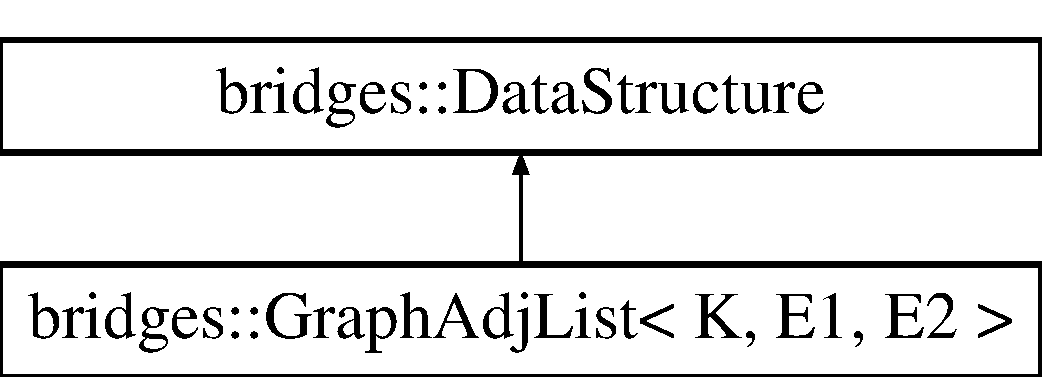
\includegraphics[height=2.000000cm]{classbridges_1_1_graph_adj_list}
\end{center}
\end{figure}
\subsection*{Public Member Functions}
\begin{DoxyCompactItemize}
\item 
virtual \mbox{\hyperlink{classbridges_1_1_graph_adj_list_af7acceab0f85c75de56cf2fc74b3690b}{$\sim$\+Graph\+Adj\+List}} () override
\item 
virtual const string \mbox{\hyperlink{classbridges_1_1_graph_adj_list_ab1aeeed39ac0e0f66a677e7b0e722030}{get\+D\+Stype}} () const override
\item 
void \mbox{\hyperlink{classbridges_1_1_graph_adj_list_a55565a4aff573c6a7751d7845cdfd5f2}{add\+Vertex}} (const K \&k, const E1 \&e=E1())
\item 
void \mbox{\hyperlink{classbridges_1_1_graph_adj_list_acd9a3bf8e544a6b78e75acd6bf1d57ee}{add\+Edge}} (const K \&src, const K \&dest, const unsigned int \&wt, const E2 \&data=E2())
\item 
E1 \mbox{\hyperlink{classbridges_1_1_graph_adj_list_a2b419a910171cafac2b71ba9f8692e5e}{get\+Vertex\+Data}} (const K \&src)
\item 
void \mbox{\hyperlink{classbridges_1_1_graph_adj_list_aa30a944a429e0422cbe0ddd7bdbd353b}{set\+Vertex\+Data}} (const K \&src, E1 \&data)
\item 
E2 \& \mbox{\hyperlink{classbridges_1_1_graph_adj_list_a3e4b21d0ff4b277502b2bb10e57df3c7}{get\+Edge\+Data}} (const K \&src, const K \&dest)
\item 
void \mbox{\hyperlink{classbridges_1_1_graph_adj_list_ac507940618b400d792c29b69fc9c7687}{set\+Edge\+Data}} (const K \&src, const K \&dest, E2 \&data)
\item 
unordered\+\_\+map$<$ K, \mbox{\hyperlink{classbridges_1_1_element}{Element}}$<$ E1 $>$ $\ast$ $>$ $\ast$ \mbox{\hyperlink{classbridges_1_1_graph_adj_list_a157c80e2bd439572f4f80e8850700297}{get\+Vertices}} ()
\item 
const \mbox{\hyperlink{classbridges_1_1_element}{Element}}$<$ E1 $>$ $\ast$ \mbox{\hyperlink{classbridges_1_1_graph_adj_list_a9a222bfc1d37f459caac60508b816fb6}{get\+Vertex}} (const K \&key) const
\item 
\mbox{\hyperlink{classbridges_1_1_element}{Element}}$<$ E1 $>$ $\ast$ \mbox{\hyperlink{classbridges_1_1_graph_adj_list_a8ba3aefe8e118ce8d8d6fab807e494c1}{get\+Vertex}} (const K \&key)
\item 
const unordered\+\_\+map$<$ K, \mbox{\hyperlink{classbridges_1_1_s_lelement}{S\+Lelement}}$<$ \mbox{\hyperlink{classbridges_1_1_edge}{Edge}}$<$ K, E2 $>$ $>$ $\ast$ $>$ \& \mbox{\hyperlink{classbridges_1_1_graph_adj_list_ac26efd5d2e57a8b8881c57e515e80bcf}{get\+Adjacency\+List}} () const
\item 
\mbox{\hyperlink{classbridges_1_1_s_lelement}{S\+Lelement}}$<$ \mbox{\hyperlink{classbridges_1_1_edge}{Edge}}$<$ K, E2 $>$ $>$ $\ast$ \mbox{\hyperlink{classbridges_1_1_graph_adj_list_ab9eb791b7c242742ac832121f297acdc}{get\+Adjacency\+List}} (const K \&k)
\item 
\mbox{\hyperlink{classbridges_1_1_element_visualizer}{Element\+Visualizer}} $\ast$ \mbox{\hyperlink{classbridges_1_1_graph_adj_list_a1c2c773a13dbd1fddd55bc2642c08574}{get\+Visualizer}} (const K \&k)
\item 
\mbox{\hyperlink{classbridges_1_1_link_visualizer}{Link\+Visualizer}} $\ast$ \mbox{\hyperlink{classbridges_1_1_graph_adj_list_a6e065b1411388387ff1e4df9227ce480}{get\+Link\+Visualizer}} (const K \&k1, const K \&k2)
\end{DoxyCompactItemize}


\subsection{Detailed Description}
\subsubsection*{template$<$typename K, typename E1 = K, typename E2 = E1$>$\newline
class bridges\+::\+Graph\+Adj\+List$<$ K, E1, E2 $>$}

This class provides methods to represent adjacency list based graphs. 

The class is simply a wrapper around the C++ S\+TL unordered\+\_\+map class and thus derives all its operations from it.

{\bfseries Generic Parameters\+:} \begin{DoxyVerb}     K:  used as an index to retrieve vertices,
     E1: data type used to store vertex specific information,
     E2: data type used to store edge specific information
\end{DoxyVerb}


\begin{DoxyAuthor}{Author}
Kalpathi Subramanian 
\end{DoxyAuthor}
\begin{DoxyDate}{Date}
Last modified 4/22/18 
\end{DoxyDate}


\subsection{Constructor \& Destructor Documentation}
\mbox{\Hypertarget{classbridges_1_1_graph_adj_list_af7acceab0f85c75de56cf2fc74b3690b}\label{classbridges_1_1_graph_adj_list_af7acceab0f85c75de56cf2fc74b3690b}} 
\index{bridges\+::\+Graph\+Adj\+List@{bridges\+::\+Graph\+Adj\+List}!````~Graph\+Adj\+List@{$\sim$\+Graph\+Adj\+List}}
\index{````~Graph\+Adj\+List@{$\sim$\+Graph\+Adj\+List}!bridges\+::\+Graph\+Adj\+List@{bridges\+::\+Graph\+Adj\+List}}
\subsubsection{\texorpdfstring{$\sim$\+Graph\+Adj\+List()}{~GraphAdjList()}}
{\footnotesize\ttfamily template$<$typename K , typename E1  = K, typename E2  = E1$>$ \\
virtual \mbox{\hyperlink{classbridges_1_1_graph_adj_list}{bridges\+::\+Graph\+Adj\+List}}$<$ K, E1, E2 $>$\+::$\sim$\mbox{\hyperlink{classbridges_1_1_graph_adj_list}{Graph\+Adj\+List}} (\begin{DoxyParamCaption}{ }\end{DoxyParamCaption})\hspace{0.3cm}{\ttfamily [inline]}, {\ttfamily [override]}, {\ttfamily [virtual]}}



\subsection{Member Function Documentation}
\mbox{\Hypertarget{classbridges_1_1_graph_adj_list_acd9a3bf8e544a6b78e75acd6bf1d57ee}\label{classbridges_1_1_graph_adj_list_acd9a3bf8e544a6b78e75acd6bf1d57ee}} 
\index{bridges\+::\+Graph\+Adj\+List@{bridges\+::\+Graph\+Adj\+List}!add\+Edge@{add\+Edge}}
\index{add\+Edge@{add\+Edge}!bridges\+::\+Graph\+Adj\+List@{bridges\+::\+Graph\+Adj\+List}}
\subsubsection{\texorpdfstring{add\+Edge()}{addEdge()}}
{\footnotesize\ttfamily template$<$typename K , typename E1  = K, typename E2  = E1$>$ \\
void \mbox{\hyperlink{classbridges_1_1_graph_adj_list}{bridges\+::\+Graph\+Adj\+List}}$<$ K, E1, E2 $>$\+::add\+Edge (\begin{DoxyParamCaption}\item[{const K \&}]{src,  }\item[{const K \&}]{dest,  }\item[{const unsigned int \&}]{wt,  }\item[{const E2 \&}]{data = {\ttfamily E2()} }\end{DoxyParamCaption})\hspace{0.3cm}{\ttfamily [inline]}}

Sets the edge from \char`\"{}src\char`\"{} to \char`\"{}dest\char`\"{}, weight to \char`\"{}wt\char`\"{} and data to \char`\"{}data\char`\"{}. Note. This function adds the edge regardless of the contents of the adjacency list; its the user\textquotesingle{}s responsibility to ensure there are no duplicates and ensure consistency.


\begin{DoxyParams}{Parameters}
{\em src} & The key of the source Vertex \\
\hline
{\em dest} & The key of the destination Vertex \\
\hline
{\em wt} & The weight of the edge \\
\hline
{\em data} & The edge data \\
\hline
\end{DoxyParams}

\begin{DoxyExceptions}{Exceptions}
{\em out\+\_\+of\+\_\+range} & If \char`\"{}src\char`\"{} or \char`\"{}dest\char`\"{} is non-\/existenet within this graph \\
\hline
{\em bad\+\_\+alloc} & If allocation of a graph adjacency list item failed \\
\hline
\end{DoxyExceptions}
\mbox{\Hypertarget{classbridges_1_1_graph_adj_list_a55565a4aff573c6a7751d7845cdfd5f2}\label{classbridges_1_1_graph_adj_list_a55565a4aff573c6a7751d7845cdfd5f2}} 
\index{bridges\+::\+Graph\+Adj\+List@{bridges\+::\+Graph\+Adj\+List}!add\+Vertex@{add\+Vertex}}
\index{add\+Vertex@{add\+Vertex}!bridges\+::\+Graph\+Adj\+List@{bridges\+::\+Graph\+Adj\+List}}
\subsubsection{\texorpdfstring{add\+Vertex()}{addVertex()}}
{\footnotesize\ttfamily template$<$typename K , typename E1  = K, typename E2  = E1$>$ \\
void \mbox{\hyperlink{classbridges_1_1_graph_adj_list}{bridges\+::\+Graph\+Adj\+List}}$<$ K, E1, E2 $>$\+::add\+Vertex (\begin{DoxyParamCaption}\item[{const K \&}]{k,  }\item[{const E1 \&}]{e = {\ttfamily E1()} }\end{DoxyParamCaption})\hspace{0.3cm}{\ttfamily [inline]}}

Adds a vertex of key \char`\"{}k\char`\"{} and value \char`\"{}e\char`\"{} to the graph, and initializes its adjacency list; If this key already exists then this will not create a new vertex.


\begin{DoxyParams}{Parameters}
{\em k} & The vertex key \\
\hline
{\em e} & The vertex data \\
\hline
\end{DoxyParams}
\mbox{\Hypertarget{classbridges_1_1_graph_adj_list_ac26efd5d2e57a8b8881c57e515e80bcf}\label{classbridges_1_1_graph_adj_list_ac26efd5d2e57a8b8881c57e515e80bcf}} 
\index{bridges\+::\+Graph\+Adj\+List@{bridges\+::\+Graph\+Adj\+List}!get\+Adjacency\+List@{get\+Adjacency\+List}}
\index{get\+Adjacency\+List@{get\+Adjacency\+List}!bridges\+::\+Graph\+Adj\+List@{bridges\+::\+Graph\+Adj\+List}}
\subsubsection{\texorpdfstring{get\+Adjacency\+List()}{getAdjacencyList()}\hspace{0.1cm}{\footnotesize\ttfamily [1/2]}}
{\footnotesize\ttfamily template$<$typename K , typename E1  = K, typename E2  = E1$>$ \\
const unordered\+\_\+map$<$K, \mbox{\hyperlink{classbridges_1_1_s_lelement}{S\+Lelement}}$<$\mbox{\hyperlink{classbridges_1_1_edge}{Edge}}$<$K, E2$>$ $>$$\ast$$>$\& \mbox{\hyperlink{classbridges_1_1_graph_adj_list}{bridges\+::\+Graph\+Adj\+List}}$<$ K, E1, E2 $>$\+::get\+Adjacency\+List (\begin{DoxyParamCaption}{ }\end{DoxyParamCaption}) const\hspace{0.3cm}{\ttfamily [inline]}}

\begin{DoxyReturn}{Returns}
The adjacency list of the graph 
\end{DoxyReturn}
\mbox{\Hypertarget{classbridges_1_1_graph_adj_list_ab9eb791b7c242742ac832121f297acdc}\label{classbridges_1_1_graph_adj_list_ab9eb791b7c242742ac832121f297acdc}} 
\index{bridges\+::\+Graph\+Adj\+List@{bridges\+::\+Graph\+Adj\+List}!get\+Adjacency\+List@{get\+Adjacency\+List}}
\index{get\+Adjacency\+List@{get\+Adjacency\+List}!bridges\+::\+Graph\+Adj\+List@{bridges\+::\+Graph\+Adj\+List}}
\subsubsection{\texorpdfstring{get\+Adjacency\+List()}{getAdjacencyList()}\hspace{0.1cm}{\footnotesize\ttfamily [2/2]}}
{\footnotesize\ttfamily template$<$typename K , typename E1  = K, typename E2  = E1$>$ \\
\mbox{\hyperlink{classbridges_1_1_s_lelement}{S\+Lelement}}$<$\mbox{\hyperlink{classbridges_1_1_edge}{Edge}}$<$K, E2$>$ $>$$\ast$ \mbox{\hyperlink{classbridges_1_1_graph_adj_list}{bridges\+::\+Graph\+Adj\+List}}$<$ K, E1, E2 $>$\+::get\+Adjacency\+List (\begin{DoxyParamCaption}\item[{const K \&}]{k }\end{DoxyParamCaption})\hspace{0.3cm}{\ttfamily [inline]}}

Returns adjacency list of a vertex with name k


\begin{DoxyParams}{Parameters}
{\em k} & The key of the source vertex \\
\hline
\end{DoxyParams}

\begin{DoxyExceptions}{Exceptions}
{\em out\+\_\+of\+\_\+range} & If key is non-\/existent within this graph\\
\hline
\end{DoxyExceptions}
\begin{DoxyReturn}{Returns}
The adjacency list of key \char`\"{}k\char`\"{} 
\end{DoxyReturn}
\mbox{\Hypertarget{classbridges_1_1_graph_adj_list_ab1aeeed39ac0e0f66a677e7b0e722030}\label{classbridges_1_1_graph_adj_list_ab1aeeed39ac0e0f66a677e7b0e722030}} 
\index{bridges\+::\+Graph\+Adj\+List@{bridges\+::\+Graph\+Adj\+List}!get\+D\+Stype@{get\+D\+Stype}}
\index{get\+D\+Stype@{get\+D\+Stype}!bridges\+::\+Graph\+Adj\+List@{bridges\+::\+Graph\+Adj\+List}}
\subsubsection{\texorpdfstring{get\+D\+Stype()}{getDStype()}}
{\footnotesize\ttfamily template$<$typename K , typename E1  = K, typename E2  = E1$>$ \\
virtual const string \mbox{\hyperlink{classbridges_1_1_graph_adj_list}{bridges\+::\+Graph\+Adj\+List}}$<$ K, E1, E2 $>$\+::get\+D\+Stype (\begin{DoxyParamCaption}{ }\end{DoxyParamCaption}) const\hspace{0.3cm}{\ttfamily [inline]}, {\ttfamily [override]}, {\ttfamily [virtual]}}

\begin{DoxyReturn}{Returns}
The string representation of this data structure type 
\end{DoxyReturn}


Implements \mbox{\hyperlink{classbridges_1_1_data_structure_a957a63b106e340bc753620c650632bdc}{bridges\+::\+Data\+Structure}}.

\mbox{\Hypertarget{classbridges_1_1_graph_adj_list_a3e4b21d0ff4b277502b2bb10e57df3c7}\label{classbridges_1_1_graph_adj_list_a3e4b21d0ff4b277502b2bb10e57df3c7}} 
\index{bridges\+::\+Graph\+Adj\+List@{bridges\+::\+Graph\+Adj\+List}!get\+Edge\+Data@{get\+Edge\+Data}}
\index{get\+Edge\+Data@{get\+Edge\+Data}!bridges\+::\+Graph\+Adj\+List@{bridges\+::\+Graph\+Adj\+List}}
\subsubsection{\texorpdfstring{get\+Edge\+Data()}{getEdgeData()}}
{\footnotesize\ttfamily template$<$typename K , typename E1  = K, typename E2  = E1$>$ \\
E2\& \mbox{\hyperlink{classbridges_1_1_graph_adj_list}{bridges\+::\+Graph\+Adj\+List}}$<$ K, E1, E2 $>$\+::get\+Edge\+Data (\begin{DoxyParamCaption}\item[{const K \&}]{src,  }\item[{const K \&}]{dest }\end{DoxyParamCaption})\hspace{0.3cm}{\ttfamily [inline]}}

Gets edge data for the edge from \char`\"{}src\char`\"{} to \char`\"{}dest\char`\"{}


\begin{DoxyParams}{Parameters}
{\em src} & The key of the source Vertex \\
\hline
{\em dest} & The key of the destination Vertex\\
\hline
\end{DoxyParams}
\begin{DoxyReturn}{Returns}
E2 edge specific data 
\end{DoxyReturn}
\mbox{\Hypertarget{classbridges_1_1_graph_adj_list_a6e065b1411388387ff1e4df9227ce480}\label{classbridges_1_1_graph_adj_list_a6e065b1411388387ff1e4df9227ce480}} 
\index{bridges\+::\+Graph\+Adj\+List@{bridges\+::\+Graph\+Adj\+List}!get\+Link\+Visualizer@{get\+Link\+Visualizer}}
\index{get\+Link\+Visualizer@{get\+Link\+Visualizer}!bridges\+::\+Graph\+Adj\+List@{bridges\+::\+Graph\+Adj\+List}}
\subsubsection{\texorpdfstring{get\+Link\+Visualizer()}{getLinkVisualizer()}}
{\footnotesize\ttfamily template$<$typename K , typename E1  = K, typename E2  = E1$>$ \\
\mbox{\hyperlink{classbridges_1_1_link_visualizer}{Link\+Visualizer}}$\ast$ \mbox{\hyperlink{classbridges_1_1_graph_adj_list}{bridges\+::\+Graph\+Adj\+List}}$<$ K, E1, E2 $>$\+::get\+Link\+Visualizer (\begin{DoxyParamCaption}\item[{const K \&}]{k1,  }\item[{const K \&}]{k2 }\end{DoxyParamCaption})\hspace{0.3cm}{\ttfamily [inline]}}

Returns the link visualizer corresponding to two graph nodes with an existing link; error returned if no link exists.


\begin{DoxyParams}{Parameters}
{\em k1} & The key of the link source vertex \\
\hline
{\em k2} & The key of the link destination vertex\\
\hline
\end{DoxyParams}
\begin{DoxyReturn}{Returns}
the visualizer that controls the attributes of this link 
\end{DoxyReturn}
\mbox{\Hypertarget{classbridges_1_1_graph_adj_list_a9a222bfc1d37f459caac60508b816fb6}\label{classbridges_1_1_graph_adj_list_a9a222bfc1d37f459caac60508b816fb6}} 
\index{bridges\+::\+Graph\+Adj\+List@{bridges\+::\+Graph\+Adj\+List}!get\+Vertex@{get\+Vertex}}
\index{get\+Vertex@{get\+Vertex}!bridges\+::\+Graph\+Adj\+List@{bridges\+::\+Graph\+Adj\+List}}
\subsubsection{\texorpdfstring{get\+Vertex()}{getVertex()}\hspace{0.1cm}{\footnotesize\ttfamily [1/2]}}
{\footnotesize\ttfamily template$<$typename K , typename E1  = K, typename E2  = E1$>$ \\
const \mbox{\hyperlink{classbridges_1_1_element}{Element}}$<$E1$>$$\ast$ \mbox{\hyperlink{classbridges_1_1_graph_adj_list}{bridges\+::\+Graph\+Adj\+List}}$<$ K, E1, E2 $>$\+::get\+Vertex (\begin{DoxyParamCaption}\item[{const K \&}]{key }\end{DoxyParamCaption}) const\hspace{0.3cm}{\ttfamily [inline]}}

\begin{DoxyReturn}{Returns}
the requested vertex of this graph 
\end{DoxyReturn}
\mbox{\Hypertarget{classbridges_1_1_graph_adj_list_a8ba3aefe8e118ce8d8d6fab807e494c1}\label{classbridges_1_1_graph_adj_list_a8ba3aefe8e118ce8d8d6fab807e494c1}} 
\index{bridges\+::\+Graph\+Adj\+List@{bridges\+::\+Graph\+Adj\+List}!get\+Vertex@{get\+Vertex}}
\index{get\+Vertex@{get\+Vertex}!bridges\+::\+Graph\+Adj\+List@{bridges\+::\+Graph\+Adj\+List}}
\subsubsection{\texorpdfstring{get\+Vertex()}{getVertex()}\hspace{0.1cm}{\footnotesize\ttfamily [2/2]}}
{\footnotesize\ttfamily template$<$typename K , typename E1  = K, typename E2  = E1$>$ \\
\mbox{\hyperlink{classbridges_1_1_element}{Element}}$<$E1$>$$\ast$ \mbox{\hyperlink{classbridges_1_1_graph_adj_list}{bridges\+::\+Graph\+Adj\+List}}$<$ K, E1, E2 $>$\+::get\+Vertex (\begin{DoxyParamCaption}\item[{const K \&}]{key }\end{DoxyParamCaption})\hspace{0.3cm}{\ttfamily [inline]}}

\begin{DoxyReturn}{Returns}
the requested vertex of this graph
\end{DoxyReturn}
non-\/const version \mbox{\Hypertarget{classbridges_1_1_graph_adj_list_a2b419a910171cafac2b71ba9f8692e5e}\label{classbridges_1_1_graph_adj_list_a2b419a910171cafac2b71ba9f8692e5e}} 
\index{bridges\+::\+Graph\+Adj\+List@{bridges\+::\+Graph\+Adj\+List}!get\+Vertex\+Data@{get\+Vertex\+Data}}
\index{get\+Vertex\+Data@{get\+Vertex\+Data}!bridges\+::\+Graph\+Adj\+List@{bridges\+::\+Graph\+Adj\+List}}
\subsubsection{\texorpdfstring{get\+Vertex\+Data()}{getVertexData()}}
{\footnotesize\ttfamily template$<$typename K , typename E1  = K, typename E2  = E1$>$ \\
E1 \mbox{\hyperlink{classbridges_1_1_graph_adj_list}{bridges\+::\+Graph\+Adj\+List}}$<$ K, E1, E2 $>$\+::get\+Vertex\+Data (\begin{DoxyParamCaption}\item[{const K \&}]{src }\end{DoxyParamCaption})\hspace{0.3cm}{\ttfamily [inline]}}

Gets vertex data for a graph vertex


\begin{DoxyParams}{Parameters}
{\em src} & The key of the source vertex\\
\hline
\end{DoxyParams}
\begin{DoxyReturn}{Returns}
E1 vertex specific data 
\end{DoxyReturn}
\mbox{\Hypertarget{classbridges_1_1_graph_adj_list_a157c80e2bd439572f4f80e8850700297}\label{classbridges_1_1_graph_adj_list_a157c80e2bd439572f4f80e8850700297}} 
\index{bridges\+::\+Graph\+Adj\+List@{bridges\+::\+Graph\+Adj\+List}!get\+Vertices@{get\+Vertices}}
\index{get\+Vertices@{get\+Vertices}!bridges\+::\+Graph\+Adj\+List@{bridges\+::\+Graph\+Adj\+List}}
\subsubsection{\texorpdfstring{get\+Vertices()}{getVertices()}}
{\footnotesize\ttfamily template$<$typename K , typename E1  = K, typename E2  = E1$>$ \\
unordered\+\_\+map$<$K, \mbox{\hyperlink{classbridges_1_1_element}{Element}}$<$E1$>$$\ast$$>$$\ast$ \mbox{\hyperlink{classbridges_1_1_graph_adj_list}{bridges\+::\+Graph\+Adj\+List}}$<$ K, E1, E2 $>$\+::get\+Vertices (\begin{DoxyParamCaption}{ }\end{DoxyParamCaption})\hspace{0.3cm}{\ttfamily [inline]}}

\begin{DoxyReturn}{Returns}
The vertex list of this graph 
\end{DoxyReturn}
\mbox{\Hypertarget{classbridges_1_1_graph_adj_list_a1c2c773a13dbd1fddd55bc2642c08574}\label{classbridges_1_1_graph_adj_list_a1c2c773a13dbd1fddd55bc2642c08574}} 
\index{bridges\+::\+Graph\+Adj\+List@{bridges\+::\+Graph\+Adj\+List}!get\+Visualizer@{get\+Visualizer}}
\index{get\+Visualizer@{get\+Visualizer}!bridges\+::\+Graph\+Adj\+List@{bridges\+::\+Graph\+Adj\+List}}
\subsubsection{\texorpdfstring{get\+Visualizer()}{getVisualizer()}}
{\footnotesize\ttfamily template$<$typename K , typename E1  = K, typename E2  = E1$>$ \\
\mbox{\hyperlink{classbridges_1_1_element_visualizer}{Element\+Visualizer}}$\ast$ \mbox{\hyperlink{classbridges_1_1_graph_adj_list}{bridges\+::\+Graph\+Adj\+List}}$<$ K, E1, E2 $>$\+::get\+Visualizer (\begin{DoxyParamCaption}\item[{const K \&}]{k }\end{DoxyParamCaption})\hspace{0.3cm}{\ttfamily [inline]}}

Returns the visualizer corresponding to a graph vertex; convenient method to set attributes of the graph vertex


\begin{DoxyParams}{Parameters}
{\em k} & The key of the graph vertex\\
\hline
\end{DoxyParams}
\begin{DoxyReturn}{Returns}
the visualizer that controls the attributes of this node 
\end{DoxyReturn}
\mbox{\Hypertarget{classbridges_1_1_graph_adj_list_ac507940618b400d792c29b69fc9c7687}\label{classbridges_1_1_graph_adj_list_ac507940618b400d792c29b69fc9c7687}} 
\index{bridges\+::\+Graph\+Adj\+List@{bridges\+::\+Graph\+Adj\+List}!set\+Edge\+Data@{set\+Edge\+Data}}
\index{set\+Edge\+Data@{set\+Edge\+Data}!bridges\+::\+Graph\+Adj\+List@{bridges\+::\+Graph\+Adj\+List}}
\subsubsection{\texorpdfstring{set\+Edge\+Data()}{setEdgeData()}}
{\footnotesize\ttfamily template$<$typename K , typename E1  = K, typename E2  = E1$>$ \\
void \mbox{\hyperlink{classbridges_1_1_graph_adj_list}{bridges\+::\+Graph\+Adj\+List}}$<$ K, E1, E2 $>$\+::set\+Edge\+Data (\begin{DoxyParamCaption}\item[{const K \&}]{src,  }\item[{const K \&}]{dest,  }\item[{E2 \&}]{data }\end{DoxyParamCaption})\hspace{0.3cm}{\ttfamily [inline]}}

Loads edge specific information for the edge from \char`\"{}src\char`\"{} to \char`\"{}dest\char`\"{}


\begin{DoxyParams}{Parameters}
{\em src} & The key of the source Vertex \\
\hline
{\em dest} & The key of the destination Vertex \\
\hline
\end{DoxyParams}
\mbox{\Hypertarget{classbridges_1_1_graph_adj_list_aa30a944a429e0422cbe0ddd7bdbd353b}\label{classbridges_1_1_graph_adj_list_aa30a944a429e0422cbe0ddd7bdbd353b}} 
\index{bridges\+::\+Graph\+Adj\+List@{bridges\+::\+Graph\+Adj\+List}!set\+Vertex\+Data@{set\+Vertex\+Data}}
\index{set\+Vertex\+Data@{set\+Vertex\+Data}!bridges\+::\+Graph\+Adj\+List@{bridges\+::\+Graph\+Adj\+List}}
\subsubsection{\texorpdfstring{set\+Vertex\+Data()}{setVertexData()}}
{\footnotesize\ttfamily template$<$typename K , typename E1  = K, typename E2  = E1$>$ \\
void \mbox{\hyperlink{classbridges_1_1_graph_adj_list}{bridges\+::\+Graph\+Adj\+List}}$<$ K, E1, E2 $>$\+::set\+Vertex\+Data (\begin{DoxyParamCaption}\item[{const K \&}]{src,  }\item[{E1 \&}]{data }\end{DoxyParamCaption})\hspace{0.3cm}{\ttfamily [inline]}}

Loads vertex specific information for a graph vertex


\begin{DoxyParams}{Parameters}
{\em src} & The key of the source Vertex \\
\hline
\end{DoxyParams}


The documentation for this class was generated from the following files\+:\begin{DoxyCompactItemize}
\item 
/\+Users/kalpathi/gr/bridges/client/cxx/bridges17/src/\mbox{\hyperlink{_element_8h}{Element.\+h}}\item 
/\+Users/kalpathi/gr/bridges/client/cxx/bridges17/src/\mbox{\hyperlink{_graph_adj_list_8h}{Graph\+Adj\+List.\+h}}\end{DoxyCompactItemize}

\hypertarget{classbridges_1_1_graph_adj_matrix}{}\section{bridges\+:\+:Graph\+Adj\+Matrix$<$ K, E $>$ Class Template Reference}
\label{classbridges_1_1_graph_adj_matrix}\index{bridges\+::\+Graph\+Adj\+Matrix$<$ K, E $>$@{bridges\+::\+Graph\+Adj\+Matrix$<$ K, E $>$}}


This class provides methods to represent adjacency matrix based graphs.  




{\ttfamily \#include $<$Element.\+h$>$}

Inheritance diagram for bridges\+:\+:Graph\+Adj\+Matrix$<$ K, E $>$\+:\begin{figure}[H]
\begin{center}
\leavevmode
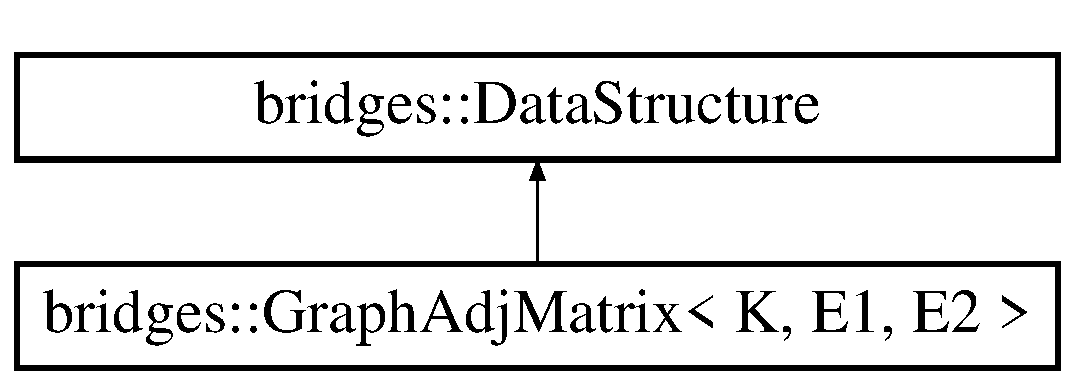
\includegraphics[height=2.000000cm]{classbridges_1_1_graph_adj_matrix}
\end{center}
\end{figure}
\subsection*{Public Member Functions}
\begin{DoxyCompactItemize}
\item 
virtual const string \hyperlink{classbridges_1_1_graph_adj_matrix_a174dc9df7605c66abe4610943a793c99}{get\+D\+Stype} () const override
\item 
void \hyperlink{classbridges_1_1_graph_adj_matrix_a7d0c2f70e4030d903b4ecea2ac3b564a}{add\+Vertex} (const K \&k, const E \&e=E())
\item 
void \hyperlink{classbridges_1_1_graph_adj_matrix_a98accd921cace9f9d9cff0925aa1e3b2}{add\+Edge} (const K \&src, const K \&dest, const unsigned int \&wt)
\item 
const unordered\+\_\+map$<$ K, unordered\+\_\+map$<$ K, int $>$ $>$ \& \hyperlink{classbridges_1_1_graph_adj_matrix_a074539c082e58f3ed89e2b5ad281ede3}{get\+Matrix} () const
\item 
const unordered\+\_\+map$<$ K, \hyperlink{classbridges_1_1_element}{Element}$<$ E $>$ $\ast$ $>$ \& \hyperlink{classbridges_1_1_graph_adj_matrix_a66ca65ceecdb2b30209749330c0a8971}{get\+Vertices} () const
\end{DoxyCompactItemize}


\subsection{Detailed Description}
\subsubsection*{template$<$typename K, typename E$>$\newline
class bridges\+::\+Graph\+Adj\+Matrix$<$ K, E $>$}

This class provides methods to represent adjacency matrix based graphs. 

The class is simply a wrapper around the C++ S\+TL unordered\+\_\+map class and thus derives all its operations from it. Given the use of operator overloading, the adjacency matrix implementation is almost identical to a normal array representation, except that any ordered type can be used to index into the matrix.

Generic Parameters\+: K that is used as an index, E the application data type

\begin{DoxyAuthor}{Author}
Kalpathi Subramanian, Dakota Carmer 
\end{DoxyAuthor}
\begin{DoxyDate}{Date}
6/29/15, 7/10/16, 11/27/16 
\end{DoxyDate}


\subsection{Member Function Documentation}
\hypertarget{classbridges_1_1_graph_adj_matrix_a98accd921cace9f9d9cff0925aa1e3b2}{}\label{classbridges_1_1_graph_adj_matrix_a98accd921cace9f9d9cff0925aa1e3b2} 
\index{bridges\+::\+Graph\+Adj\+Matrix@{bridges\+::\+Graph\+Adj\+Matrix}!add\+Edge@{add\+Edge}}
\index{add\+Edge@{add\+Edge}!bridges\+::\+Graph\+Adj\+Matrix@{bridges\+::\+Graph\+Adj\+Matrix}}
\subsubsection{\texorpdfstring{add\+Edge()}{addEdge()}}
{\footnotesize\ttfamily template$<$typename K , typename E $>$ \\
void \hyperlink{classbridges_1_1_graph_adj_matrix}{bridges\+::\+Graph\+Adj\+Matrix}$<$ K, E $>$\+::add\+Edge (\begin{DoxyParamCaption}\item[{const K \&}]{src,  }\item[{const K \&}]{dest,  }\item[{const unsigned int \&}]{wt }\end{DoxyParamCaption})\hspace{0.3cm}{\ttfamily [inline]}}

Sets the weight of the edge from \char`\"{}src\char`\"{} to \char`\"{}dest\char`\"{}, to \char`\"{}wt\char`\"{}. This will overwrite the existing edge weight.


\begin{DoxyParams}{Parameters}
{\em src} & The key of the source Vertex \\
\hline
{\em dest} & The key of the destination Vertex \\
\hline
{\em wt} & The weight of the edge \\
\hline
\end{DoxyParams}

\begin{DoxyExceptions}{Exceptions}
{\em out\+\_\+of\+\_\+range} & If \char`\"{}src\char`\"{} or \char`\"{}dest\char`\"{} is non-\/existent within this graph \\
\hline
\end{DoxyExceptions}
\hypertarget{classbridges_1_1_graph_adj_matrix_a7d0c2f70e4030d903b4ecea2ac3b564a}{}\label{classbridges_1_1_graph_adj_matrix_a7d0c2f70e4030d903b4ecea2ac3b564a} 
\index{bridges\+::\+Graph\+Adj\+Matrix@{bridges\+::\+Graph\+Adj\+Matrix}!add\+Vertex@{add\+Vertex}}
\index{add\+Vertex@{add\+Vertex}!bridges\+::\+Graph\+Adj\+Matrix@{bridges\+::\+Graph\+Adj\+Matrix}}
\subsubsection{\texorpdfstring{add\+Vertex()}{addVertex()}}
{\footnotesize\ttfamily template$<$typename K , typename E $>$ \\
void \hyperlink{classbridges_1_1_graph_adj_matrix}{bridges\+::\+Graph\+Adj\+Matrix}$<$ K, E $>$\+::add\+Vertex (\begin{DoxyParamCaption}\item[{const K \&}]{k,  }\item[{const E \&}]{e = {\ttfamily E()} }\end{DoxyParamCaption})\hspace{0.3cm}{\ttfamily [inline]}}

Adds a vertex of key \char`\"{}k\char`\"{} and value \char`\"{}e\char`\"{} to the graph. Sets all of its edges to be of weight 0.


\begin{DoxyParams}{Parameters}
{\em k} & Vertex key \\
\hline
{\em e} & Vertex data \\
\hline
\end{DoxyParams}
\hypertarget{classbridges_1_1_graph_adj_matrix_a174dc9df7605c66abe4610943a793c99}{}\label{classbridges_1_1_graph_adj_matrix_a174dc9df7605c66abe4610943a793c99} 
\index{bridges\+::\+Graph\+Adj\+Matrix@{bridges\+::\+Graph\+Adj\+Matrix}!get\+D\+Stype@{get\+D\+Stype}}
\index{get\+D\+Stype@{get\+D\+Stype}!bridges\+::\+Graph\+Adj\+Matrix@{bridges\+::\+Graph\+Adj\+Matrix}}
\subsubsection{\texorpdfstring{get\+D\+Stype()}{getDStype()}}
{\footnotesize\ttfamily template$<$typename K , typename E $>$ \\
virtual const string \hyperlink{classbridges_1_1_graph_adj_matrix}{bridges\+::\+Graph\+Adj\+Matrix}$<$ K, E $>$\+::get\+D\+Stype (\begin{DoxyParamCaption}{ }\end{DoxyParamCaption}) const\hspace{0.3cm}{\ttfamily [inline]}, {\ttfamily [override]}, {\ttfamily [virtual]}}

\begin{DoxyReturn}{Returns}
The string representation of this data structure type 
\end{DoxyReturn}


Implements \hyperlink{classbridges_1_1_data_structure_a957a63b106e340bc753620c650632bdc}{bridges\+::\+Data\+Structure}.

\hypertarget{classbridges_1_1_graph_adj_matrix_a074539c082e58f3ed89e2b5ad281ede3}{}\label{classbridges_1_1_graph_adj_matrix_a074539c082e58f3ed89e2b5ad281ede3} 
\index{bridges\+::\+Graph\+Adj\+Matrix@{bridges\+::\+Graph\+Adj\+Matrix}!get\+Matrix@{get\+Matrix}}
\index{get\+Matrix@{get\+Matrix}!bridges\+::\+Graph\+Adj\+Matrix@{bridges\+::\+Graph\+Adj\+Matrix}}
\subsubsection{\texorpdfstring{get\+Matrix()}{getMatrix()}}
{\footnotesize\ttfamily template$<$typename K , typename E $>$ \\
const unordered\+\_\+map$<$K, unordered\+\_\+map$<$K, int$>$ $>$\& \hyperlink{classbridges_1_1_graph_adj_matrix}{bridges\+::\+Graph\+Adj\+Matrix}$<$ K, E $>$\+::get\+Matrix (\begin{DoxyParamCaption}{ }\end{DoxyParamCaption}) const\hspace{0.3cm}{\ttfamily [inline]}}

\begin{DoxyReturn}{Returns}
The matrix of this graphs edges 
\end{DoxyReturn}
\hypertarget{classbridges_1_1_graph_adj_matrix_a66ca65ceecdb2b30209749330c0a8971}{}\label{classbridges_1_1_graph_adj_matrix_a66ca65ceecdb2b30209749330c0a8971} 
\index{bridges\+::\+Graph\+Adj\+Matrix@{bridges\+::\+Graph\+Adj\+Matrix}!get\+Vertices@{get\+Vertices}}
\index{get\+Vertices@{get\+Vertices}!bridges\+::\+Graph\+Adj\+Matrix@{bridges\+::\+Graph\+Adj\+Matrix}}
\subsubsection{\texorpdfstring{get\+Vertices()}{getVertices()}}
{\footnotesize\ttfamily template$<$typename K , typename E $>$ \\
const unordered\+\_\+map$<$K, \hyperlink{classbridges_1_1_element}{Element}$<$E$>$ $\ast$$>$\& \hyperlink{classbridges_1_1_graph_adj_matrix}{bridges\+::\+Graph\+Adj\+Matrix}$<$ K, E $>$\+::get\+Vertices (\begin{DoxyParamCaption}{ }\end{DoxyParamCaption}) const\hspace{0.3cm}{\ttfamily [inline]}}

\begin{DoxyReturn}{Returns}
The graph verticies 
\end{DoxyReturn}


The documentation for this class was generated from the following files\+:\begin{DoxyCompactItemize}
\item 
/\+Users/kalpathi/gr/bridges/client/cxx/git-\/cxx/src/\hyperlink{_element_8h}{Element.\+h}\item 
/\+Users/kalpathi/gr/bridges/client/cxx/git-\/cxx/src/\hyperlink{_graph_adj_matrix_8h}{Graph\+Adj\+Matrix.\+h}\end{DoxyCompactItemize}

\hypertarget{classbridges_1_1_grid}{}\section{bridges\+:\+:Grid$<$ E $>$ Class Template Reference}
\label{classbridges_1_1_grid}\index{bridges\+::\+Grid$<$ E $>$@{bridges\+::\+Grid$<$ E $>$}}


This is a class in B\+R\+I\+D\+G\+ES for representing an (n x n) grid.  




{\ttfamily \#include $<$Grid.\+h$>$}

Inheritance diagram for bridges\+:\+:Grid$<$ E $>$\+:\begin{figure}[H]
\begin{center}
\leavevmode
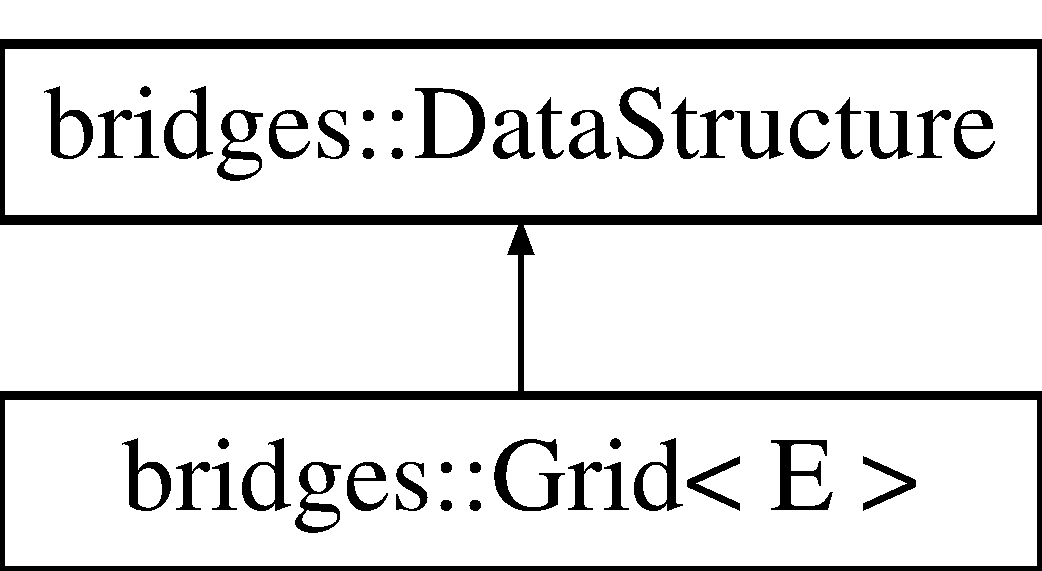
\includegraphics[height=2.000000cm]{classbridges_1_1_grid}
\end{center}
\end{figure}
\subsection*{Public Member Functions}
\begin{DoxyCompactItemize}
\item 
virtual const string \mbox{\hyperlink{classbridges_1_1_grid_ab701d081de4f7ffafb15966758dd5446}{get\+D\+Stype}} () const override
\item 
\mbox{\hyperlink{classbridges_1_1_grid_af8bb9244c4c713f2325af6d4754ad1e9}{Grid}} (int rows, int cols)
\item 
\mbox{\hyperlink{classbridges_1_1_grid_a711e05a933c2a11c9e2775c74e6cf80d}{Grid}} ()
\item 
\mbox{\hyperlink{classbridges_1_1_grid_ad5c6c5e87eb40446ac794c5479937f87}{Grid}} (int $\ast$size)
\item 
virtual \mbox{\hyperlink{classbridges_1_1_grid_a46cc94397ea38211349b10e3629b2590}{$\sim$\+Grid}} ()
\item 
void \mbox{\hyperlink{classbridges_1_1_grid_a8e5e4d92097f9d1481a14219eb5cc5a8}{set\+Dimensions}} (int rows, int cols)
\item 
int $\ast$ \mbox{\hyperlink{classbridges_1_1_grid_ad21e4fc94483ef822fda9b74a52b9f48}{get\+Dimensions}} ()
\item 
E \mbox{\hyperlink{classbridges_1_1_grid_aab69e77d9e1a51eabcf29c9c229cd35f}{get}} (int row, int col)
\item 
void \mbox{\hyperlink{classbridges_1_1_grid_acd750e5886349488257aba85f0b06f6f}{set}} (int row, int col, E val)
\item 
\mbox{\hyperlink{classbridges_1_1_grid_af3b18d3a6b302c200154e869337cc85b}{Grid}} (const \mbox{\hyperlink{classbridges_1_1_grid}{Grid}} \&)=delete
\item 
\mbox{\hyperlink{classbridges_1_1_grid}{Grid}} \& \mbox{\hyperlink{classbridges_1_1_grid_ab79fc10a9ebd55dd3565ca1ea6933b13}{operator=}} (const \mbox{\hyperlink{classbridges_1_1_grid}{Grid}} \&)=delete
\end{DoxyCompactItemize}
\subsection*{Protected Attributes}
\begin{DoxyCompactItemize}
\item 
E $\ast$$\ast$ \mbox{\hyperlink{classbridges_1_1_grid_aea6c38498d477f09dc03906ee6fb6e19}{grid}} = nullptr
\item 
int \mbox{\hyperlink{classbridges_1_1_grid_af7c3a077b54e3346621e54276c1fa13e}{grid\+Size}} \mbox{[}2\mbox{]}
\item 
int \mbox{\hyperlink{classbridges_1_1_grid_a800909a94e0affac82da79cf3e6d03e5}{max\+Grid\+Size}} \mbox{[}2\mbox{]} = \{1080, 1920\}
\end{DoxyCompactItemize}


\subsection{Detailed Description}
\subsubsection*{template$<$typename E$>$\newline
class bridges\+::\+Grid$<$ E $>$}

This is a class in B\+R\+I\+D\+G\+ES for representing an (n x n) grid. 

This class will be useful in applications such as image processing, board games, etc.

\begin{DoxyAuthor}{Author}
David Burlinson, C++ port Kalpathi Subramanian
\end{DoxyAuthor}

\begin{DoxyParams}{Parameters}
{\em E} & \\
\hline
\end{DoxyParams}


\subsection{Constructor \& Destructor Documentation}
\mbox{\Hypertarget{classbridges_1_1_grid_af8bb9244c4c713f2325af6d4754ad1e9}\label{classbridges_1_1_grid_af8bb9244c4c713f2325af6d4754ad1e9}} 
\index{bridges\+::\+Grid@{bridges\+::\+Grid}!Grid@{Grid}}
\index{Grid@{Grid}!bridges\+::\+Grid@{bridges\+::\+Grid}}
\subsubsection{\texorpdfstring{Grid()}{Grid()}\hspace{0.1cm}{\footnotesize\ttfamily [1/4]}}
{\footnotesize\ttfamily template$<$typename E$>$ \\
\mbox{\hyperlink{classbridges_1_1_grid}{bridges\+::\+Grid}}$<$ E $>$\+::\mbox{\hyperlink{classbridges_1_1_grid}{Grid}} (\begin{DoxyParamCaption}\item[{int}]{rows,  }\item[{int}]{cols }\end{DoxyParamCaption})\hspace{0.3cm}{\ttfamily [inline]}}

\mbox{\hyperlink{classbridges_1_1_grid}{Grid}} constructors \mbox{\Hypertarget{classbridges_1_1_grid_a711e05a933c2a11c9e2775c74e6cf80d}\label{classbridges_1_1_grid_a711e05a933c2a11c9e2775c74e6cf80d}} 
\index{bridges\+::\+Grid@{bridges\+::\+Grid}!Grid@{Grid}}
\index{Grid@{Grid}!bridges\+::\+Grid@{bridges\+::\+Grid}}
\subsubsection{\texorpdfstring{Grid()}{Grid()}\hspace{0.1cm}{\footnotesize\ttfamily [2/4]}}
{\footnotesize\ttfamily template$<$typename E$>$ \\
\mbox{\hyperlink{classbridges_1_1_grid}{bridges\+::\+Grid}}$<$ E $>$\+::\mbox{\hyperlink{classbridges_1_1_grid}{Grid}} (\begin{DoxyParamCaption}{ }\end{DoxyParamCaption})\hspace{0.3cm}{\ttfamily [inline]}}

\mbox{\Hypertarget{classbridges_1_1_grid_ad5c6c5e87eb40446ac794c5479937f87}\label{classbridges_1_1_grid_ad5c6c5e87eb40446ac794c5479937f87}} 
\index{bridges\+::\+Grid@{bridges\+::\+Grid}!Grid@{Grid}}
\index{Grid@{Grid}!bridges\+::\+Grid@{bridges\+::\+Grid}}
\subsubsection{\texorpdfstring{Grid()}{Grid()}\hspace{0.1cm}{\footnotesize\ttfamily [3/4]}}
{\footnotesize\ttfamily template$<$typename E$>$ \\
\mbox{\hyperlink{classbridges_1_1_grid}{bridges\+::\+Grid}}$<$ E $>$\+::\mbox{\hyperlink{classbridges_1_1_grid}{Grid}} (\begin{DoxyParamCaption}\item[{int $\ast$}]{size }\end{DoxyParamCaption})\hspace{0.3cm}{\ttfamily [inline]}, {\ttfamily [explicit]}}

\mbox{\Hypertarget{classbridges_1_1_grid_a46cc94397ea38211349b10e3629b2590}\label{classbridges_1_1_grid_a46cc94397ea38211349b10e3629b2590}} 
\index{bridges\+::\+Grid@{bridges\+::\+Grid}!````~Grid@{$\sim$\+Grid}}
\index{````~Grid@{$\sim$\+Grid}!bridges\+::\+Grid@{bridges\+::\+Grid}}
\subsubsection{\texorpdfstring{$\sim$\+Grid()}{~Grid()}}
{\footnotesize\ttfamily template$<$typename E$>$ \\
virtual \mbox{\hyperlink{classbridges_1_1_grid}{bridges\+::\+Grid}}$<$ E $>$\+::$\sim$\mbox{\hyperlink{classbridges_1_1_grid}{Grid}} (\begin{DoxyParamCaption}{ }\end{DoxyParamCaption})\hspace{0.3cm}{\ttfamily [inline]}, {\ttfamily [virtual]}}

\mbox{\Hypertarget{classbridges_1_1_grid_af3b18d3a6b302c200154e869337cc85b}\label{classbridges_1_1_grid_af3b18d3a6b302c200154e869337cc85b}} 
\index{bridges\+::\+Grid@{bridges\+::\+Grid}!Grid@{Grid}}
\index{Grid@{Grid}!bridges\+::\+Grid@{bridges\+::\+Grid}}
\subsubsection{\texorpdfstring{Grid()}{Grid()}\hspace{0.1cm}{\footnotesize\ttfamily [4/4]}}
{\footnotesize\ttfamily template$<$typename E$>$ \\
\mbox{\hyperlink{classbridges_1_1_grid}{bridges\+::\+Grid}}$<$ E $>$\+::\mbox{\hyperlink{classbridges_1_1_grid}{Grid}} (\begin{DoxyParamCaption}\item[{const \mbox{\hyperlink{classbridges_1_1_grid}{Grid}}$<$ E $>$ \&}]{ }\end{DoxyParamCaption})\hspace{0.3cm}{\ttfamily [delete]}}



\subsection{Member Function Documentation}
\mbox{\Hypertarget{classbridges_1_1_grid_aab69e77d9e1a51eabcf29c9c229cd35f}\label{classbridges_1_1_grid_aab69e77d9e1a51eabcf29c9c229cd35f}} 
\index{bridges\+::\+Grid@{bridges\+::\+Grid}!get@{get}}
\index{get@{get}!bridges\+::\+Grid@{bridges\+::\+Grid}}
\subsubsection{\texorpdfstring{get()}{get()}}
{\footnotesize\ttfamily template$<$typename E$>$ \\
E \mbox{\hyperlink{classbridges_1_1_grid}{bridges\+::\+Grid}}$<$ E $>$\+::get (\begin{DoxyParamCaption}\item[{int}]{row,  }\item[{int}]{col }\end{DoxyParamCaption})\hspace{0.3cm}{\ttfamily [inline]}}

\mbox{\Hypertarget{classbridges_1_1_grid_ad21e4fc94483ef822fda9b74a52b9f48}\label{classbridges_1_1_grid_ad21e4fc94483ef822fda9b74a52b9f48}} 
\index{bridges\+::\+Grid@{bridges\+::\+Grid}!get\+Dimensions@{get\+Dimensions}}
\index{get\+Dimensions@{get\+Dimensions}!bridges\+::\+Grid@{bridges\+::\+Grid}}
\subsubsection{\texorpdfstring{get\+Dimensions()}{getDimensions()}}
{\footnotesize\ttfamily template$<$typename E$>$ \\
int$\ast$ \mbox{\hyperlink{classbridges_1_1_grid}{bridges\+::\+Grid}}$<$ E $>$\+::get\+Dimensions (\begin{DoxyParamCaption}{ }\end{DoxyParamCaption})\hspace{0.3cm}{\ttfamily [inline]}}

\mbox{\Hypertarget{classbridges_1_1_grid_ab701d081de4f7ffafb15966758dd5446}\label{classbridges_1_1_grid_ab701d081de4f7ffafb15966758dd5446}} 
\index{bridges\+::\+Grid@{bridges\+::\+Grid}!get\+D\+Stype@{get\+D\+Stype}}
\index{get\+D\+Stype@{get\+D\+Stype}!bridges\+::\+Grid@{bridges\+::\+Grid}}
\subsubsection{\texorpdfstring{get\+D\+Stype()}{getDStype()}}
{\footnotesize\ttfamily template$<$typename E$>$ \\
virtual const string \mbox{\hyperlink{classbridges_1_1_grid}{bridges\+::\+Grid}}$<$ E $>$\+::get\+D\+Stype (\begin{DoxyParamCaption}{ }\end{DoxyParamCaption}) const\hspace{0.3cm}{\ttfamily [inline]}, {\ttfamily [override]}, {\ttfamily [virtual]}}

\begin{DoxyReturn}{Returns}
The string representation of this data structure type 
\end{DoxyReturn}


Implements \mbox{\hyperlink{classbridges_1_1_data_structure_a957a63b106e340bc753620c650632bdc}{bridges\+::\+Data\+Structure}}.



Reimplemented in \mbox{\hyperlink{classbridges_1_1_color_grid_a6bb93994dade8e79a197459532dad153}{bridges\+::\+Color\+Grid}}.

\mbox{\Hypertarget{classbridges_1_1_grid_ab79fc10a9ebd55dd3565ca1ea6933b13}\label{classbridges_1_1_grid_ab79fc10a9ebd55dd3565ca1ea6933b13}} 
\index{bridges\+::\+Grid@{bridges\+::\+Grid}!operator=@{operator=}}
\index{operator=@{operator=}!bridges\+::\+Grid@{bridges\+::\+Grid}}
\subsubsection{\texorpdfstring{operator=()}{operator=()}}
{\footnotesize\ttfamily template$<$typename E$>$ \\
\mbox{\hyperlink{classbridges_1_1_grid}{Grid}}\& \mbox{\hyperlink{classbridges_1_1_grid}{bridges\+::\+Grid}}$<$ E $>$\+::operator= (\begin{DoxyParamCaption}\item[{const \mbox{\hyperlink{classbridges_1_1_grid}{Grid}}$<$ E $>$ \&}]{ }\end{DoxyParamCaption})\hspace{0.3cm}{\ttfamily [delete]}}

\mbox{\Hypertarget{classbridges_1_1_grid_acd750e5886349488257aba85f0b06f6f}\label{classbridges_1_1_grid_acd750e5886349488257aba85f0b06f6f}} 
\index{bridges\+::\+Grid@{bridges\+::\+Grid}!set@{set}}
\index{set@{set}!bridges\+::\+Grid@{bridges\+::\+Grid}}
\subsubsection{\texorpdfstring{set()}{set()}}
{\footnotesize\ttfamily template$<$typename E$>$ \\
void \mbox{\hyperlink{classbridges_1_1_grid}{bridges\+::\+Grid}}$<$ E $>$\+::set (\begin{DoxyParamCaption}\item[{int}]{row,  }\item[{int}]{col,  }\item[{E}]{val }\end{DoxyParamCaption})\hspace{0.3cm}{\ttfamily [inline]}}

\mbox{\Hypertarget{classbridges_1_1_grid_a8e5e4d92097f9d1481a14219eb5cc5a8}\label{classbridges_1_1_grid_a8e5e4d92097f9d1481a14219eb5cc5a8}} 
\index{bridges\+::\+Grid@{bridges\+::\+Grid}!set\+Dimensions@{set\+Dimensions}}
\index{set\+Dimensions@{set\+Dimensions}!bridges\+::\+Grid@{bridges\+::\+Grid}}
\subsubsection{\texorpdfstring{set\+Dimensions()}{setDimensions()}}
{\footnotesize\ttfamily template$<$typename E$>$ \\
void \mbox{\hyperlink{classbridges_1_1_grid}{bridges\+::\+Grid}}$<$ E $>$\+::set\+Dimensions (\begin{DoxyParamCaption}\item[{int}]{rows,  }\item[{int}]{cols }\end{DoxyParamCaption})\hspace{0.3cm}{\ttfamily [inline]}}



\subsection{Member Data Documentation}
\mbox{\Hypertarget{classbridges_1_1_grid_aea6c38498d477f09dc03906ee6fb6e19}\label{classbridges_1_1_grid_aea6c38498d477f09dc03906ee6fb6e19}} 
\index{bridges\+::\+Grid@{bridges\+::\+Grid}!grid@{grid}}
\index{grid@{grid}!bridges\+::\+Grid@{bridges\+::\+Grid}}
\subsubsection{\texorpdfstring{grid}{grid}}
{\footnotesize\ttfamily template$<$typename E$>$ \\
E$\ast$$\ast$ \mbox{\hyperlink{classbridges_1_1_grid}{bridges\+::\+Grid}}$<$ E $>$\+::grid = nullptr\hspace{0.3cm}{\ttfamily [protected]}}

\mbox{\Hypertarget{classbridges_1_1_grid_af7c3a077b54e3346621e54276c1fa13e}\label{classbridges_1_1_grid_af7c3a077b54e3346621e54276c1fa13e}} 
\index{bridges\+::\+Grid@{bridges\+::\+Grid}!grid\+Size@{grid\+Size}}
\index{grid\+Size@{grid\+Size}!bridges\+::\+Grid@{bridges\+::\+Grid}}
\subsubsection{\texorpdfstring{grid\+Size}{gridSize}}
{\footnotesize\ttfamily template$<$typename E$>$ \\
int \mbox{\hyperlink{classbridges_1_1_grid}{bridges\+::\+Grid}}$<$ E $>$\+::grid\+Size\mbox{[}2\mbox{]}\hspace{0.3cm}{\ttfamily [protected]}}

\mbox{\Hypertarget{classbridges_1_1_grid_a800909a94e0affac82da79cf3e6d03e5}\label{classbridges_1_1_grid_a800909a94e0affac82da79cf3e6d03e5}} 
\index{bridges\+::\+Grid@{bridges\+::\+Grid}!max\+Grid\+Size@{max\+Grid\+Size}}
\index{max\+Grid\+Size@{max\+Grid\+Size}!bridges\+::\+Grid@{bridges\+::\+Grid}}
\subsubsection{\texorpdfstring{max\+Grid\+Size}{maxGridSize}}
{\footnotesize\ttfamily template$<$typename E$>$ \\
int \mbox{\hyperlink{classbridges_1_1_grid}{bridges\+::\+Grid}}$<$ E $>$\+::max\+Grid\+Size\mbox{[}2\mbox{]} = \{1080, 1920\}\hspace{0.3cm}{\ttfamily [protected]}}



The documentation for this class was generated from the following file\+:\begin{DoxyCompactItemize}
\item 
/\+Users/kalpathi/gr/bridges/client/cxx/bridges17/src/\mbox{\hyperlink{_grid_8h}{Grid.\+h}}\end{DoxyCompactItemize}

\hypertarget{classbridges_1_1_gutenberg_book}{}\section{bridges\+:\+:Gutenberg\+Book Class Reference}
\label{classbridges_1_1_gutenberg_book}\index{bridges\+::\+Gutenberg\+Book@{bridges\+::\+Gutenberg\+Book}}


A Gutenberg Book object metadata only, used along with the books data source.  




{\ttfamily \#include $<$Gutenberg\+Book.\+h$>$}

\subsection*{Public Member Functions}
\begin{DoxyCompactItemize}
\item 
\hyperlink{classbridges_1_1_gutenberg_book_a289c167dd11eed17cce39a59931f246c}{Gutenberg\+Book} ()
\item 
\hyperlink{classbridges_1_1_gutenberg_book_ab792768f0f2567835e90659f163f4438}{Gutenberg\+Book} (string author\+Name, int author\+Birth, int author\+Death, string title, vector$<$ string $>$ lang, vector$<$ string $>$ genre, vector$<$ string $>$ subject, int num\+Chars, int num\+Words, int num\+Sentences, int num\+Difficult\+Words, string url, int downloads)
\item 
string \hyperlink{classbridges_1_1_gutenberg_book_aa323f15acc05fd74bb59cd3c182ca686}{get\+Author\+Name} ()
\item 
void \hyperlink{classbridges_1_1_gutenberg_book_ab7b3a1d3398b75100b8d3fb7936b3ac9}{set\+Author\+Name} (string author\+Name)
\item 
int \hyperlink{classbridges_1_1_gutenberg_book_a86f4ea70ec32fd1cce772910b9dcc9a6}{get\+Author\+Birth} ()
\item 
void \hyperlink{classbridges_1_1_gutenberg_book_a33ac2e6063319064006fa72b6fcfb0dc}{set\+Author\+Birth} (int author\+Birth)
\item 
int \hyperlink{classbridges_1_1_gutenberg_book_a82ae9b4815b25f8e7b337f143f1cf828}{get\+Author\+Death} ()
\item 
void \hyperlink{classbridges_1_1_gutenberg_book_acf1e81a3b635fb939bc6af772a61fd3c}{set\+Author\+Death} (int author\+Death)
\item 
string \hyperlink{classbridges_1_1_gutenberg_book_a1ef4a40396485a78480f99ca3b490db0}{get\+Title} ()
\item 
void \hyperlink{classbridges_1_1_gutenberg_book_a5038252948e5f173dad4926c0970c5d3}{set\+Title} (string title)
\item 
vector$<$ string $>$ \hyperlink{classbridges_1_1_gutenberg_book_ac2eabdf4c650bc3720dcf5b030a59d0d}{get\+Lang} ()
\item 
void \hyperlink{classbridges_1_1_gutenberg_book_ab8cf27c1e496eb34d1e74e8343b4a466}{set\+Lang} (vector$<$ string $>$ lang)
\item 
vector$<$ string $>$ \hyperlink{classbridges_1_1_gutenberg_book_a7caa2af2fdd0af98e95ed4fad74efdd7}{get\+Genre} ()
\item 
void \hyperlink{classbridges_1_1_gutenberg_book_a2b81b6cf785ea9dfef0a1b1e15331b38}{set\+Genre} (vector$<$ string $>$ genre)
\item 
vector$<$ string $>$ \hyperlink{classbridges_1_1_gutenberg_book_aa005000e827d8b3dd208ab269906f8ed}{get\+Subject} ()
\item 
void \hyperlink{classbridges_1_1_gutenberg_book_aa640bef3156b13c8ca510e0a280b1c5f}{set\+Subject} (vector$<$ string $>$ subject)
\item 
string \hyperlink{classbridges_1_1_gutenberg_book_a1456d456f75c689b06d80b7e2d0f46e3}{get\+U\+R\+L} ()
\item 
void \hyperlink{classbridges_1_1_gutenberg_book_a4a5fa52c405170b57535cd0fcde5e3cf}{set\+U\+R\+L} (string url)
\item 
int \hyperlink{classbridges_1_1_gutenberg_book_aa86b5c97b78ef0f745723a7245ee05f2}{get\+Num\+Chars} ()
\item 
void \hyperlink{classbridges_1_1_gutenberg_book_a65cb7af6360e56a684e0606593846780}{set\+Num\+Chars} (int num\+Chars)
\item 
int \hyperlink{classbridges_1_1_gutenberg_book_aadb4dc37374a7b3be6b7b4def4726d5b}{get\+Num\+Words} ()
\item 
void \hyperlink{classbridges_1_1_gutenberg_book_a34dafee1fb976f1da102d40f33a08ecf}{set\+Num\+Words} (int num\+Words)
\item 
int \hyperlink{classbridges_1_1_gutenberg_book_a059066390328e09949ea5fdb456a5c43}{get\+Num\+Sentences} ()
\item 
void \hyperlink{classbridges_1_1_gutenberg_book_a368e71eaea48375104f172e0ae17527d}{set\+Num\+Sentences} (int num\+Sentences)
\item 
int \hyperlink{classbridges_1_1_gutenberg_book_a26f18a0274a7cebd495f3e438e9a037f}{get\+Num\+Difficult\+Words} ()
\item 
void \hyperlink{classbridges_1_1_gutenberg_book_a4397cd3b9fd6113a1e72eb7671dd9d87}{set\+Num\+Difficult\+Words} (int num\+Difficult\+Words)
\item 
int \hyperlink{classbridges_1_1_gutenberg_book_a9d11f90ed3928c075534f3712e00f011}{get\+Num\+Downloads} ()
\item 
void \hyperlink{classbridges_1_1_gutenberg_book_a6846dba9a5a78f360a0483b8685d79c1}{set\+Num\+Downloads} (int dl)
\end{DoxyCompactItemize}


\subsection{Detailed Description}
A Gutenberg Book object metadata only, used along with the books data source. 

This is a convenience class provided for users who wish to use this data source as part of their application. It provides an A\+P\+I that makes it easy to access the attributes of this data set.

Refer to tutorial examples to using this data source in data structure assignments.

\begin{DoxyAuthor}{Author}
Kalpathi Subramanian 
\end{DoxyAuthor}
\begin{DoxyDate}{Date}
2/1/17 
\end{DoxyDate}


\subsection{Constructor \& Destructor Documentation}
\hypertarget{classbridges_1_1_gutenberg_book_a289c167dd11eed17cce39a59931f246c}{}\index{bridges\+::\+Gutenberg\+Book@{bridges\+::\+Gutenberg\+Book}!Gutenberg\+Book@{Gutenberg\+Book}}
\index{Gutenberg\+Book@{Gutenberg\+Book}!bridges\+::\+Gutenberg\+Book@{bridges\+::\+Gutenberg\+Book}}
\subsubsection[{Gutenberg\+Book()}]{\setlength{\rightskip}{0pt plus 5cm}bridges\+::\+Gutenberg\+Book\+::\+Gutenberg\+Book (
\begin{DoxyParamCaption}
{}
\end{DoxyParamCaption}
)\hspace{0.3cm}{\ttfamily [inline]}}\label{classbridges_1_1_gutenberg_book_a289c167dd11eed17cce39a59931f246c}
\hypertarget{classbridges_1_1_gutenberg_book_ab792768f0f2567835e90659f163f4438}{}\index{bridges\+::\+Gutenberg\+Book@{bridges\+::\+Gutenberg\+Book}!Gutenberg\+Book@{Gutenberg\+Book}}
\index{Gutenberg\+Book@{Gutenberg\+Book}!bridges\+::\+Gutenberg\+Book@{bridges\+::\+Gutenberg\+Book}}
\subsubsection[{Gutenberg\+Book(string author\+Name, int author\+Birth, int author\+Death, string title, vector$<$ string $>$ lang, vector$<$ string $>$ genre, vector$<$ string $>$ subject, int num\+Chars, int num\+Words, int num\+Sentences, int num\+Difficult\+Words, string url, int downloads)}]{\setlength{\rightskip}{0pt plus 5cm}bridges\+::\+Gutenberg\+Book\+::\+Gutenberg\+Book (
\begin{DoxyParamCaption}
\item[{string}]{author\+Name, }
\item[{int}]{author\+Birth, }
\item[{int}]{author\+Death, }
\item[{string}]{title, }
\item[{vector$<$ string $>$}]{lang, }
\item[{vector$<$ string $>$}]{genre, }
\item[{vector$<$ string $>$}]{subject, }
\item[{int}]{num\+Chars, }
\item[{int}]{num\+Words, }
\item[{int}]{num\+Sentences, }
\item[{int}]{num\+Difficult\+Words, }
\item[{string}]{url, }
\item[{int}]{downloads}
\end{DoxyParamCaption}
)\hspace{0.3cm}{\ttfamily [inline]}}\label{classbridges_1_1_gutenberg_book_ab792768f0f2567835e90659f163f4438}


\subsection{Member Function Documentation}
\hypertarget{classbridges_1_1_gutenberg_book_a86f4ea70ec32fd1cce772910b9dcc9a6}{}\index{bridges\+::\+Gutenberg\+Book@{bridges\+::\+Gutenberg\+Book}!get\+Author\+Birth@{get\+Author\+Birth}}
\index{get\+Author\+Birth@{get\+Author\+Birth}!bridges\+::\+Gutenberg\+Book@{bridges\+::\+Gutenberg\+Book}}
\subsubsection[{get\+Author\+Birth()}]{\setlength{\rightskip}{0pt plus 5cm}int bridges\+::\+Gutenberg\+Book\+::get\+Author\+Birth (
\begin{DoxyParamCaption}
{}
\end{DoxyParamCaption}
)\hspace{0.3cm}{\ttfamily [inline]}}\label{classbridges_1_1_gutenberg_book_a86f4ea70ec32fd1cce772910b9dcc9a6}
\hypertarget{classbridges_1_1_gutenberg_book_a82ae9b4815b25f8e7b337f143f1cf828}{}\index{bridges\+::\+Gutenberg\+Book@{bridges\+::\+Gutenberg\+Book}!get\+Author\+Death@{get\+Author\+Death}}
\index{get\+Author\+Death@{get\+Author\+Death}!bridges\+::\+Gutenberg\+Book@{bridges\+::\+Gutenberg\+Book}}
\subsubsection[{get\+Author\+Death()}]{\setlength{\rightskip}{0pt plus 5cm}int bridges\+::\+Gutenberg\+Book\+::get\+Author\+Death (
\begin{DoxyParamCaption}
{}
\end{DoxyParamCaption}
)\hspace{0.3cm}{\ttfamily [inline]}}\label{classbridges_1_1_gutenberg_book_a82ae9b4815b25f8e7b337f143f1cf828}
\hypertarget{classbridges_1_1_gutenberg_book_aa323f15acc05fd74bb59cd3c182ca686}{}\index{bridges\+::\+Gutenberg\+Book@{bridges\+::\+Gutenberg\+Book}!get\+Author\+Name@{get\+Author\+Name}}
\index{get\+Author\+Name@{get\+Author\+Name}!bridges\+::\+Gutenberg\+Book@{bridges\+::\+Gutenberg\+Book}}
\subsubsection[{get\+Author\+Name()}]{\setlength{\rightskip}{0pt plus 5cm}string bridges\+::\+Gutenberg\+Book\+::get\+Author\+Name (
\begin{DoxyParamCaption}
{}
\end{DoxyParamCaption}
)\hspace{0.3cm}{\ttfamily [inline]}}\label{classbridges_1_1_gutenberg_book_aa323f15acc05fd74bb59cd3c182ca686}
\hypertarget{classbridges_1_1_gutenberg_book_a7caa2af2fdd0af98e95ed4fad74efdd7}{}\index{bridges\+::\+Gutenberg\+Book@{bridges\+::\+Gutenberg\+Book}!get\+Genre@{get\+Genre}}
\index{get\+Genre@{get\+Genre}!bridges\+::\+Gutenberg\+Book@{bridges\+::\+Gutenberg\+Book}}
\subsubsection[{get\+Genre()}]{\setlength{\rightskip}{0pt plus 5cm}vector$<$string$>$ bridges\+::\+Gutenberg\+Book\+::get\+Genre (
\begin{DoxyParamCaption}
{}
\end{DoxyParamCaption}
)\hspace{0.3cm}{\ttfamily [inline]}}\label{classbridges_1_1_gutenberg_book_a7caa2af2fdd0af98e95ed4fad74efdd7}
\hypertarget{classbridges_1_1_gutenberg_book_ac2eabdf4c650bc3720dcf5b030a59d0d}{}\index{bridges\+::\+Gutenberg\+Book@{bridges\+::\+Gutenberg\+Book}!get\+Lang@{get\+Lang}}
\index{get\+Lang@{get\+Lang}!bridges\+::\+Gutenberg\+Book@{bridges\+::\+Gutenberg\+Book}}
\subsubsection[{get\+Lang()}]{\setlength{\rightskip}{0pt plus 5cm}vector$<$string$>$ bridges\+::\+Gutenberg\+Book\+::get\+Lang (
\begin{DoxyParamCaption}
{}
\end{DoxyParamCaption}
)\hspace{0.3cm}{\ttfamily [inline]}}\label{classbridges_1_1_gutenberg_book_ac2eabdf4c650bc3720dcf5b030a59d0d}
\hypertarget{classbridges_1_1_gutenberg_book_aa86b5c97b78ef0f745723a7245ee05f2}{}\index{bridges\+::\+Gutenberg\+Book@{bridges\+::\+Gutenberg\+Book}!get\+Num\+Chars@{get\+Num\+Chars}}
\index{get\+Num\+Chars@{get\+Num\+Chars}!bridges\+::\+Gutenberg\+Book@{bridges\+::\+Gutenberg\+Book}}
\subsubsection[{get\+Num\+Chars()}]{\setlength{\rightskip}{0pt plus 5cm}int bridges\+::\+Gutenberg\+Book\+::get\+Num\+Chars (
\begin{DoxyParamCaption}
{}
\end{DoxyParamCaption}
)\hspace{0.3cm}{\ttfamily [inline]}}\label{classbridges_1_1_gutenberg_book_aa86b5c97b78ef0f745723a7245ee05f2}
\hypertarget{classbridges_1_1_gutenberg_book_a26f18a0274a7cebd495f3e438e9a037f}{}\index{bridges\+::\+Gutenberg\+Book@{bridges\+::\+Gutenberg\+Book}!get\+Num\+Difficult\+Words@{get\+Num\+Difficult\+Words}}
\index{get\+Num\+Difficult\+Words@{get\+Num\+Difficult\+Words}!bridges\+::\+Gutenberg\+Book@{bridges\+::\+Gutenberg\+Book}}
\subsubsection[{get\+Num\+Difficult\+Words()}]{\setlength{\rightskip}{0pt plus 5cm}int bridges\+::\+Gutenberg\+Book\+::get\+Num\+Difficult\+Words (
\begin{DoxyParamCaption}
{}
\end{DoxyParamCaption}
)\hspace{0.3cm}{\ttfamily [inline]}}\label{classbridges_1_1_gutenberg_book_a26f18a0274a7cebd495f3e438e9a037f}
\hypertarget{classbridges_1_1_gutenberg_book_a9d11f90ed3928c075534f3712e00f011}{}\index{bridges\+::\+Gutenberg\+Book@{bridges\+::\+Gutenberg\+Book}!get\+Num\+Downloads@{get\+Num\+Downloads}}
\index{get\+Num\+Downloads@{get\+Num\+Downloads}!bridges\+::\+Gutenberg\+Book@{bridges\+::\+Gutenberg\+Book}}
\subsubsection[{get\+Num\+Downloads()}]{\setlength{\rightskip}{0pt plus 5cm}int bridges\+::\+Gutenberg\+Book\+::get\+Num\+Downloads (
\begin{DoxyParamCaption}
{}
\end{DoxyParamCaption}
)\hspace{0.3cm}{\ttfamily [inline]}}\label{classbridges_1_1_gutenberg_book_a9d11f90ed3928c075534f3712e00f011}
\hypertarget{classbridges_1_1_gutenberg_book_a059066390328e09949ea5fdb456a5c43}{}\index{bridges\+::\+Gutenberg\+Book@{bridges\+::\+Gutenberg\+Book}!get\+Num\+Sentences@{get\+Num\+Sentences}}
\index{get\+Num\+Sentences@{get\+Num\+Sentences}!bridges\+::\+Gutenberg\+Book@{bridges\+::\+Gutenberg\+Book}}
\subsubsection[{get\+Num\+Sentences()}]{\setlength{\rightskip}{0pt plus 5cm}int bridges\+::\+Gutenberg\+Book\+::get\+Num\+Sentences (
\begin{DoxyParamCaption}
{}
\end{DoxyParamCaption}
)\hspace{0.3cm}{\ttfamily [inline]}}\label{classbridges_1_1_gutenberg_book_a059066390328e09949ea5fdb456a5c43}
\hypertarget{classbridges_1_1_gutenberg_book_aadb4dc37374a7b3be6b7b4def4726d5b}{}\index{bridges\+::\+Gutenberg\+Book@{bridges\+::\+Gutenberg\+Book}!get\+Num\+Words@{get\+Num\+Words}}
\index{get\+Num\+Words@{get\+Num\+Words}!bridges\+::\+Gutenberg\+Book@{bridges\+::\+Gutenberg\+Book}}
\subsubsection[{get\+Num\+Words()}]{\setlength{\rightskip}{0pt plus 5cm}int bridges\+::\+Gutenberg\+Book\+::get\+Num\+Words (
\begin{DoxyParamCaption}
{}
\end{DoxyParamCaption}
)\hspace{0.3cm}{\ttfamily [inline]}}\label{classbridges_1_1_gutenberg_book_aadb4dc37374a7b3be6b7b4def4726d5b}
\hypertarget{classbridges_1_1_gutenberg_book_aa005000e827d8b3dd208ab269906f8ed}{}\index{bridges\+::\+Gutenberg\+Book@{bridges\+::\+Gutenberg\+Book}!get\+Subject@{get\+Subject}}
\index{get\+Subject@{get\+Subject}!bridges\+::\+Gutenberg\+Book@{bridges\+::\+Gutenberg\+Book}}
\subsubsection[{get\+Subject()}]{\setlength{\rightskip}{0pt plus 5cm}vector$<$string$>$ bridges\+::\+Gutenberg\+Book\+::get\+Subject (
\begin{DoxyParamCaption}
{}
\end{DoxyParamCaption}
)\hspace{0.3cm}{\ttfamily [inline]}}\label{classbridges_1_1_gutenberg_book_aa005000e827d8b3dd208ab269906f8ed}
\hypertarget{classbridges_1_1_gutenberg_book_a1ef4a40396485a78480f99ca3b490db0}{}\index{bridges\+::\+Gutenberg\+Book@{bridges\+::\+Gutenberg\+Book}!get\+Title@{get\+Title}}
\index{get\+Title@{get\+Title}!bridges\+::\+Gutenberg\+Book@{bridges\+::\+Gutenberg\+Book}}
\subsubsection[{get\+Title()}]{\setlength{\rightskip}{0pt plus 5cm}string bridges\+::\+Gutenberg\+Book\+::get\+Title (
\begin{DoxyParamCaption}
{}
\end{DoxyParamCaption}
)\hspace{0.3cm}{\ttfamily [inline]}}\label{classbridges_1_1_gutenberg_book_a1ef4a40396485a78480f99ca3b490db0}
\hypertarget{classbridges_1_1_gutenberg_book_a1456d456f75c689b06d80b7e2d0f46e3}{}\index{bridges\+::\+Gutenberg\+Book@{bridges\+::\+Gutenberg\+Book}!get\+U\+R\+L@{get\+U\+R\+L}}
\index{get\+U\+R\+L@{get\+U\+R\+L}!bridges\+::\+Gutenberg\+Book@{bridges\+::\+Gutenberg\+Book}}
\subsubsection[{get\+U\+R\+L()}]{\setlength{\rightskip}{0pt plus 5cm}string bridges\+::\+Gutenberg\+Book\+::get\+U\+R\+L (
\begin{DoxyParamCaption}
{}
\end{DoxyParamCaption}
)\hspace{0.3cm}{\ttfamily [inline]}}\label{classbridges_1_1_gutenberg_book_a1456d456f75c689b06d80b7e2d0f46e3}
\hypertarget{classbridges_1_1_gutenberg_book_a33ac2e6063319064006fa72b6fcfb0dc}{}\index{bridges\+::\+Gutenberg\+Book@{bridges\+::\+Gutenberg\+Book}!set\+Author\+Birth@{set\+Author\+Birth}}
\index{set\+Author\+Birth@{set\+Author\+Birth}!bridges\+::\+Gutenberg\+Book@{bridges\+::\+Gutenberg\+Book}}
\subsubsection[{set\+Author\+Birth(int author\+Birth)}]{\setlength{\rightskip}{0pt plus 5cm}void bridges\+::\+Gutenberg\+Book\+::set\+Author\+Birth (
\begin{DoxyParamCaption}
\item[{int}]{author\+Birth}
\end{DoxyParamCaption}
)\hspace{0.3cm}{\ttfamily [inline]}}\label{classbridges_1_1_gutenberg_book_a33ac2e6063319064006fa72b6fcfb0dc}
\hypertarget{classbridges_1_1_gutenberg_book_acf1e81a3b635fb939bc6af772a61fd3c}{}\index{bridges\+::\+Gutenberg\+Book@{bridges\+::\+Gutenberg\+Book}!set\+Author\+Death@{set\+Author\+Death}}
\index{set\+Author\+Death@{set\+Author\+Death}!bridges\+::\+Gutenberg\+Book@{bridges\+::\+Gutenberg\+Book}}
\subsubsection[{set\+Author\+Death(int author\+Death)}]{\setlength{\rightskip}{0pt plus 5cm}void bridges\+::\+Gutenberg\+Book\+::set\+Author\+Death (
\begin{DoxyParamCaption}
\item[{int}]{author\+Death}
\end{DoxyParamCaption}
)\hspace{0.3cm}{\ttfamily [inline]}}\label{classbridges_1_1_gutenberg_book_acf1e81a3b635fb939bc6af772a61fd3c}
\hypertarget{classbridges_1_1_gutenberg_book_ab7b3a1d3398b75100b8d3fb7936b3ac9}{}\index{bridges\+::\+Gutenberg\+Book@{bridges\+::\+Gutenberg\+Book}!set\+Author\+Name@{set\+Author\+Name}}
\index{set\+Author\+Name@{set\+Author\+Name}!bridges\+::\+Gutenberg\+Book@{bridges\+::\+Gutenberg\+Book}}
\subsubsection[{set\+Author\+Name(string author\+Name)}]{\setlength{\rightskip}{0pt plus 5cm}void bridges\+::\+Gutenberg\+Book\+::set\+Author\+Name (
\begin{DoxyParamCaption}
\item[{string}]{author\+Name}
\end{DoxyParamCaption}
)\hspace{0.3cm}{\ttfamily [inline]}}\label{classbridges_1_1_gutenberg_book_ab7b3a1d3398b75100b8d3fb7936b3ac9}
\hypertarget{classbridges_1_1_gutenberg_book_a2b81b6cf785ea9dfef0a1b1e15331b38}{}\index{bridges\+::\+Gutenberg\+Book@{bridges\+::\+Gutenberg\+Book}!set\+Genre@{set\+Genre}}
\index{set\+Genre@{set\+Genre}!bridges\+::\+Gutenberg\+Book@{bridges\+::\+Gutenberg\+Book}}
\subsubsection[{set\+Genre(vector$<$ string $>$ genre)}]{\setlength{\rightskip}{0pt plus 5cm}void bridges\+::\+Gutenberg\+Book\+::set\+Genre (
\begin{DoxyParamCaption}
\item[{vector$<$ string $>$}]{genre}
\end{DoxyParamCaption}
)\hspace{0.3cm}{\ttfamily [inline]}}\label{classbridges_1_1_gutenberg_book_a2b81b6cf785ea9dfef0a1b1e15331b38}
\hypertarget{classbridges_1_1_gutenberg_book_ab8cf27c1e496eb34d1e74e8343b4a466}{}\index{bridges\+::\+Gutenberg\+Book@{bridges\+::\+Gutenberg\+Book}!set\+Lang@{set\+Lang}}
\index{set\+Lang@{set\+Lang}!bridges\+::\+Gutenberg\+Book@{bridges\+::\+Gutenberg\+Book}}
\subsubsection[{set\+Lang(vector$<$ string $>$ lang)}]{\setlength{\rightskip}{0pt plus 5cm}void bridges\+::\+Gutenberg\+Book\+::set\+Lang (
\begin{DoxyParamCaption}
\item[{vector$<$ string $>$}]{lang}
\end{DoxyParamCaption}
)\hspace{0.3cm}{\ttfamily [inline]}}\label{classbridges_1_1_gutenberg_book_ab8cf27c1e496eb34d1e74e8343b4a466}
\hypertarget{classbridges_1_1_gutenberg_book_a65cb7af6360e56a684e0606593846780}{}\index{bridges\+::\+Gutenberg\+Book@{bridges\+::\+Gutenberg\+Book}!set\+Num\+Chars@{set\+Num\+Chars}}
\index{set\+Num\+Chars@{set\+Num\+Chars}!bridges\+::\+Gutenberg\+Book@{bridges\+::\+Gutenberg\+Book}}
\subsubsection[{set\+Num\+Chars(int num\+Chars)}]{\setlength{\rightskip}{0pt plus 5cm}void bridges\+::\+Gutenberg\+Book\+::set\+Num\+Chars (
\begin{DoxyParamCaption}
\item[{int}]{num\+Chars}
\end{DoxyParamCaption}
)\hspace{0.3cm}{\ttfamily [inline]}}\label{classbridges_1_1_gutenberg_book_a65cb7af6360e56a684e0606593846780}
\hypertarget{classbridges_1_1_gutenberg_book_a4397cd3b9fd6113a1e72eb7671dd9d87}{}\index{bridges\+::\+Gutenberg\+Book@{bridges\+::\+Gutenberg\+Book}!set\+Num\+Difficult\+Words@{set\+Num\+Difficult\+Words}}
\index{set\+Num\+Difficult\+Words@{set\+Num\+Difficult\+Words}!bridges\+::\+Gutenberg\+Book@{bridges\+::\+Gutenberg\+Book}}
\subsubsection[{set\+Num\+Difficult\+Words(int num\+Difficult\+Words)}]{\setlength{\rightskip}{0pt plus 5cm}void bridges\+::\+Gutenberg\+Book\+::set\+Num\+Difficult\+Words (
\begin{DoxyParamCaption}
\item[{int}]{num\+Difficult\+Words}
\end{DoxyParamCaption}
)\hspace{0.3cm}{\ttfamily [inline]}}\label{classbridges_1_1_gutenberg_book_a4397cd3b9fd6113a1e72eb7671dd9d87}
\hypertarget{classbridges_1_1_gutenberg_book_a6846dba9a5a78f360a0483b8685d79c1}{}\index{bridges\+::\+Gutenberg\+Book@{bridges\+::\+Gutenberg\+Book}!set\+Num\+Downloads@{set\+Num\+Downloads}}
\index{set\+Num\+Downloads@{set\+Num\+Downloads}!bridges\+::\+Gutenberg\+Book@{bridges\+::\+Gutenberg\+Book}}
\subsubsection[{set\+Num\+Downloads(int dl)}]{\setlength{\rightskip}{0pt plus 5cm}void bridges\+::\+Gutenberg\+Book\+::set\+Num\+Downloads (
\begin{DoxyParamCaption}
\item[{int}]{dl}
\end{DoxyParamCaption}
)\hspace{0.3cm}{\ttfamily [inline]}}\label{classbridges_1_1_gutenberg_book_a6846dba9a5a78f360a0483b8685d79c1}
\hypertarget{classbridges_1_1_gutenberg_book_a368e71eaea48375104f172e0ae17527d}{}\index{bridges\+::\+Gutenberg\+Book@{bridges\+::\+Gutenberg\+Book}!set\+Num\+Sentences@{set\+Num\+Sentences}}
\index{set\+Num\+Sentences@{set\+Num\+Sentences}!bridges\+::\+Gutenberg\+Book@{bridges\+::\+Gutenberg\+Book}}
\subsubsection[{set\+Num\+Sentences(int num\+Sentences)}]{\setlength{\rightskip}{0pt plus 5cm}void bridges\+::\+Gutenberg\+Book\+::set\+Num\+Sentences (
\begin{DoxyParamCaption}
\item[{int}]{num\+Sentences}
\end{DoxyParamCaption}
)\hspace{0.3cm}{\ttfamily [inline]}}\label{classbridges_1_1_gutenberg_book_a368e71eaea48375104f172e0ae17527d}
\hypertarget{classbridges_1_1_gutenberg_book_a34dafee1fb976f1da102d40f33a08ecf}{}\index{bridges\+::\+Gutenberg\+Book@{bridges\+::\+Gutenberg\+Book}!set\+Num\+Words@{set\+Num\+Words}}
\index{set\+Num\+Words@{set\+Num\+Words}!bridges\+::\+Gutenberg\+Book@{bridges\+::\+Gutenberg\+Book}}
\subsubsection[{set\+Num\+Words(int num\+Words)}]{\setlength{\rightskip}{0pt plus 5cm}void bridges\+::\+Gutenberg\+Book\+::set\+Num\+Words (
\begin{DoxyParamCaption}
\item[{int}]{num\+Words}
\end{DoxyParamCaption}
)\hspace{0.3cm}{\ttfamily [inline]}}\label{classbridges_1_1_gutenberg_book_a34dafee1fb976f1da102d40f33a08ecf}
\hypertarget{classbridges_1_1_gutenberg_book_aa640bef3156b13c8ca510e0a280b1c5f}{}\index{bridges\+::\+Gutenberg\+Book@{bridges\+::\+Gutenberg\+Book}!set\+Subject@{set\+Subject}}
\index{set\+Subject@{set\+Subject}!bridges\+::\+Gutenberg\+Book@{bridges\+::\+Gutenberg\+Book}}
\subsubsection[{set\+Subject(vector$<$ string $>$ subject)}]{\setlength{\rightskip}{0pt plus 5cm}void bridges\+::\+Gutenberg\+Book\+::set\+Subject (
\begin{DoxyParamCaption}
\item[{vector$<$ string $>$}]{subject}
\end{DoxyParamCaption}
)\hspace{0.3cm}{\ttfamily [inline]}}\label{classbridges_1_1_gutenberg_book_aa640bef3156b13c8ca510e0a280b1c5f}
\hypertarget{classbridges_1_1_gutenberg_book_a5038252948e5f173dad4926c0970c5d3}{}\index{bridges\+::\+Gutenberg\+Book@{bridges\+::\+Gutenberg\+Book}!set\+Title@{set\+Title}}
\index{set\+Title@{set\+Title}!bridges\+::\+Gutenberg\+Book@{bridges\+::\+Gutenberg\+Book}}
\subsubsection[{set\+Title(string title)}]{\setlength{\rightskip}{0pt plus 5cm}void bridges\+::\+Gutenberg\+Book\+::set\+Title (
\begin{DoxyParamCaption}
\item[{string}]{title}
\end{DoxyParamCaption}
)\hspace{0.3cm}{\ttfamily [inline]}}\label{classbridges_1_1_gutenberg_book_a5038252948e5f173dad4926c0970c5d3}
\hypertarget{classbridges_1_1_gutenberg_book_a4a5fa52c405170b57535cd0fcde5e3cf}{}\index{bridges\+::\+Gutenberg\+Book@{bridges\+::\+Gutenberg\+Book}!set\+U\+R\+L@{set\+U\+R\+L}}
\index{set\+U\+R\+L@{set\+U\+R\+L}!bridges\+::\+Gutenberg\+Book@{bridges\+::\+Gutenberg\+Book}}
\subsubsection[{set\+U\+R\+L(string url)}]{\setlength{\rightskip}{0pt plus 5cm}void bridges\+::\+Gutenberg\+Book\+::set\+U\+R\+L (
\begin{DoxyParamCaption}
\item[{string}]{url}
\end{DoxyParamCaption}
)\hspace{0.3cm}{\ttfamily [inline]}}\label{classbridges_1_1_gutenberg_book_a4a5fa52c405170b57535cd0fcde5e3cf}


The documentation for this class was generated from the following file\+:\begin{DoxyCompactItemize}
\item 
/\+Users/krs/gr/bridges/bridges17/cxx/src/data\+\_\+src/\hyperlink{_gutenberg_book_8h}{Gutenberg\+Book.\+h}\end{DoxyCompactItemize}

\hypertarget{classbridges_1_1_kd_tree_element}{}\doxysection{bridges\+::Kd\+Tree\+Element$<$ K, E $>$ Class Template Reference}
\label{classbridges_1_1_kd_tree_element}\index{bridges::KdTreeElement$<$ K, E $>$@{bridges::KdTreeElement$<$ K, E $>$}}


This class can be used to create K-\/d Tree elements, derived from \mbox{\hyperlink{classbridges_1_1_b_s_t_element}{B\+S\+T\+Element}}. K-\/D trees can be thought of as the spatial equivalent binary search trees and operate on multiple dimensions (2D and 3D are most common). These trees serve as a representation of the underlying geometrically defined spaces. Specialized versions of these trees include quadtrees and octrees, which subdivide into equal sized quadrants octants at each level, respectively.  




{\ttfamily \#include $<$Kd\+Tree\+Element.\+h$>$}

Inheritance diagram for bridges\+::Kd\+Tree\+Element$<$ K, E $>$\+:\begin{figure}[H]
\begin{center}
\leavevmode
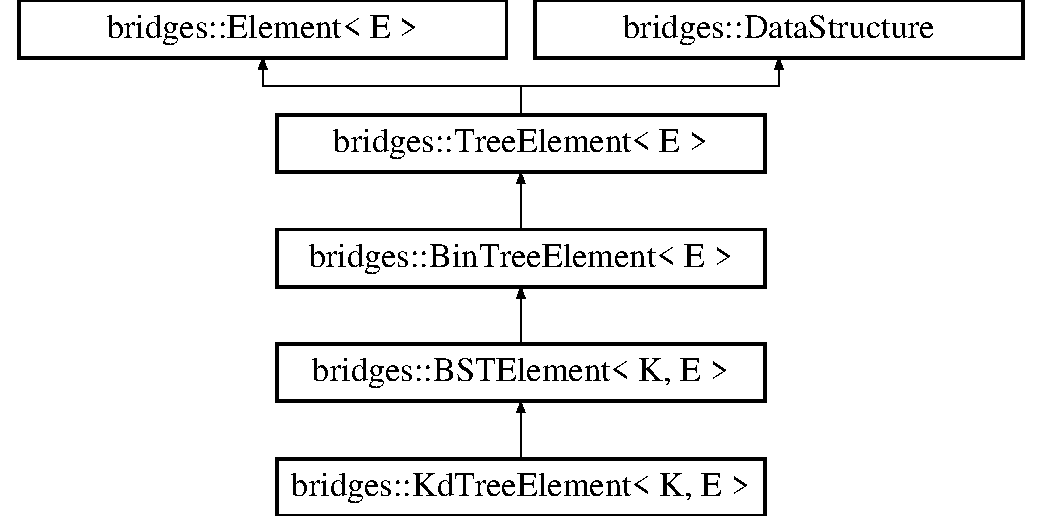
\includegraphics[height=5.000000cm]{classbridges_1_1_kd_tree_element}
\end{center}
\end{figure}
\doxysubsection*{Public Member Functions}
\begin{DoxyCompactItemize}
\item 
\mbox{\hyperlink{classbridges_1_1_kd_tree_element_a0a50d048eb39497beed77ed4b0566876}{Kd\+Tree\+Element}} (const K \&k, const int \&dim, const int \&th, const \mbox{\hyperlink{classbridges_1_1_kd_tree_element}{Kd\+Tree\+Element}} $\ast$l, \mbox{\hyperlink{classbridges_1_1_kd_tree_element}{Kd\+Tree\+Element}} $\ast$r, const E \&val=E(), const string \&lab=string())
\item 
\mbox{\hyperlink{classbridges_1_1_kd_tree_element_a50774bfe7e28ddb78bc0da8acec70eb2}{Kd\+Tree\+Element}} (const K \&k, const int \&dim, const int \&th=0, const E \&val=E(), const string \&lab=string())
\item 
virtual const string \mbox{\hyperlink{classbridges_1_1_kd_tree_element_acdd8f989986b7dd42cfacec73cf52dcb}{get\+D\+Stype}} () const override
\item 
int \mbox{\hyperlink{classbridges_1_1_kd_tree_element_aa7b34640fafac747b2e1185572e3dcc8}{get\+Dimension}} () const
\item 
void \mbox{\hyperlink{classbridges_1_1_kd_tree_element_a8c2c8503d8c8aa0db31fa834dffb60b0}{set\+Dimension}} (const int \&dim)
\item 
virtual \mbox{\hyperlink{classbridges_1_1_kd_tree_element}{Kd\+Tree\+Element}} $\ast$ \mbox{\hyperlink{classbridges_1_1_kd_tree_element_ad7db63a4f82f5252c7e0809ac6486cb4}{get\+Left}} () override
\item 
virtual const \mbox{\hyperlink{classbridges_1_1_kd_tree_element}{Kd\+Tree\+Element}} $\ast$ \mbox{\hyperlink{classbridges_1_1_kd_tree_element_ab58af4ca67cb3869c279bfc11952c070}{get\+Left}} () const override
\item 
void \mbox{\hyperlink{classbridges_1_1_kd_tree_element_a4aabf3ae1f9e77676f5c7b87181ada67}{set\+Left}} (\mbox{\hyperlink{classbridges_1_1_kd_tree_element}{Kd\+Tree\+Element}} $\ast$l)
\item 
virtual \mbox{\hyperlink{classbridges_1_1_kd_tree_element}{Kd\+Tree\+Element}} $\ast$ \mbox{\hyperlink{classbridges_1_1_kd_tree_element_a8e1090891a720231c2009d1d222471e9}{get\+Right}} () override
\item 
virtual const \mbox{\hyperlink{classbridges_1_1_kd_tree_element}{Kd\+Tree\+Element}} $\ast$ \mbox{\hyperlink{classbridges_1_1_kd_tree_element_a48e6a81eccf6d156e50865ef8066be82}{get\+Right}} () const override
\item 
void \mbox{\hyperlink{classbridges_1_1_kd_tree_element_a119124cbfcc0e792ea60cb56c0a63119}{set\+Right}} (\mbox{\hyperlink{classbridges_1_1_kd_tree_element}{Kd\+Tree\+Element}} $\ast$r)
\end{DoxyCompactItemize}
\doxysubsection*{Protected Member Functions}
\begin{DoxyCompactItemize}
\item 
virtual const string \mbox{\hyperlink{classbridges_1_1_kd_tree_element_ad8aa2d89689f33691063fee9c601e2cb}{get\+Element\+Representation}} () const override
\end{DoxyCompactItemize}
\doxysubsection*{Additional Inherited Members}


\doxysubsection{Detailed Description}
\subsubsection*{template$<$typename K, typename E$>$\newline
class bridges\+::\+Kd\+Tree\+Element$<$ K, E $>$}

This class can be used to create K-\/d Tree elements, derived from \mbox{\hyperlink{classbridges_1_1_b_s_t_element}{B\+S\+T\+Element}}. K-\/D trees can be thought of as the spatial equivalent binary search trees and operate on multiple dimensions (2D and 3D are most common). These trees serve as a representation of the underlying geometrically defined spaces. Specialized versions of these trees include quadtrees and octrees, which subdivide into equal sized quadrants octants at each level, respectively. 

This class extends the \mbox{\hyperlink{classbridges_1_1_b_s_t_element}{B\+S\+T\+Element}} class by adding a dimension property. It also includes a thickness property for displaying the partitioning lines generated by the convex decomposition.

convenient to generate visual representation to allow for use in a binary search tree implementation.

Generic Parameters\+: K that is the search key type -\/ this is usually a number, integer or float E the application data type

\begin{DoxyAuthor}{Author}
Kalpathi Subramanian 
\end{DoxyAuthor}
\begin{DoxyDate}{Date}
6/18/15, 7/17/16 
\end{DoxyDate}


\doxysubsection{Constructor \& Destructor Documentation}
\mbox{\Hypertarget{classbridges_1_1_kd_tree_element_a0a50d048eb39497beed77ed4b0566876}\label{classbridges_1_1_kd_tree_element_a0a50d048eb39497beed77ed4b0566876}} 
\index{bridges::KdTreeElement$<$ K, E $>$@{bridges::KdTreeElement$<$ K, E $>$}!KdTreeElement@{KdTreeElement}}
\index{KdTreeElement@{KdTreeElement}!bridges::KdTreeElement$<$ K, E $>$@{bridges::KdTreeElement$<$ K, E $>$}}
\doxysubsubsection{\texorpdfstring{KdTreeElement()}{KdTreeElement()}\hspace{0.1cm}{\footnotesize\ttfamily [1/2]}}
{\footnotesize\ttfamily template$<$typename K , typename E $>$ \\
\mbox{\hyperlink{classbridges_1_1_kd_tree_element}{bridges\+::\+Kd\+Tree\+Element}}$<$ K, E $>$\+::\mbox{\hyperlink{classbridges_1_1_kd_tree_element}{Kd\+Tree\+Element}} (\begin{DoxyParamCaption}\item[{const K \&}]{k,  }\item[{const int \&}]{dim,  }\item[{const int \&}]{th,  }\item[{const \mbox{\hyperlink{classbridges_1_1_kd_tree_element}{Kd\+Tree\+Element}}$<$ K, E $>$ $\ast$}]{l,  }\item[{\mbox{\hyperlink{classbridges_1_1_kd_tree_element}{Kd\+Tree\+Element}}$<$ K, E $>$ $\ast$}]{r,  }\item[{const E \&}]{val = {\ttfamily E()},  }\item[{const string \&}]{lab = {\ttfamily string()} }\end{DoxyParamCaption})\hspace{0.3cm}{\ttfamily [inline]}}

Constructs a \mbox{\hyperlink{classbridges_1_1_kd_tree_element}{Kd\+Tree\+Element}} with the provided value, label, key, left and right Kd\+Tree elements. The defaults will be used if not provided.


\begin{DoxyParams}{Parameters}
{\em k} & The key for ordering \\
\hline
{\em val} & The data to hold \\
\hline
{\em lab} & The label to show \\
\hline
{\em l} & The left Kd\+Tree \mbox{\hyperlink{classbridges_1_1_element}{Element}} \\
\hline
{\em r} & The right Kd\+Tree \mbox{\hyperlink{classbridges_1_1_element}{Element}} \\
\hline
\end{DoxyParams}
\mbox{\Hypertarget{classbridges_1_1_kd_tree_element_a50774bfe7e28ddb78bc0da8acec70eb2}\label{classbridges_1_1_kd_tree_element_a50774bfe7e28ddb78bc0da8acec70eb2}} 
\index{bridges::KdTreeElement$<$ K, E $>$@{bridges::KdTreeElement$<$ K, E $>$}!KdTreeElement@{KdTreeElement}}
\index{KdTreeElement@{KdTreeElement}!bridges::KdTreeElement$<$ K, E $>$@{bridges::KdTreeElement$<$ K, E $>$}}
\doxysubsubsection{\texorpdfstring{KdTreeElement()}{KdTreeElement()}\hspace{0.1cm}{\footnotesize\ttfamily [2/2]}}
{\footnotesize\ttfamily template$<$typename K , typename E $>$ \\
\mbox{\hyperlink{classbridges_1_1_kd_tree_element}{bridges\+::\+Kd\+Tree\+Element}}$<$ K, E $>$\+::\mbox{\hyperlink{classbridges_1_1_kd_tree_element}{Kd\+Tree\+Element}} (\begin{DoxyParamCaption}\item[{const K \&}]{k,  }\item[{const int \&}]{dim,  }\item[{const int \&}]{th = {\ttfamily 0},  }\item[{const E \&}]{val = {\ttfamily E()},  }\item[{const string \&}]{lab = {\ttfamily string()} }\end{DoxyParamCaption})\hspace{0.3cm}{\ttfamily [inline]}}

Constructs a \mbox{\hyperlink{classbridges_1_1_b_s_t_element}{B\+S\+T\+Element}} with the provided value, label, key, setting the left and right B\+S\+T\+Elements to N\+U\+LL. The defaults will be used if not provided.


\begin{DoxyParams}{Parameters}
{\em val} & The data to hold \\
\hline
{\em lab} & The label to show \\
\hline
{\em k} & The key for ordering \\
\hline
\end{DoxyParams}


\doxysubsection{Member Function Documentation}
\mbox{\Hypertarget{classbridges_1_1_kd_tree_element_aa7b34640fafac747b2e1185572e3dcc8}\label{classbridges_1_1_kd_tree_element_aa7b34640fafac747b2e1185572e3dcc8}} 
\index{bridges::KdTreeElement$<$ K, E $>$@{bridges::KdTreeElement$<$ K, E $>$}!getDimension@{getDimension}}
\index{getDimension@{getDimension}!bridges::KdTreeElement$<$ K, E $>$@{bridges::KdTreeElement$<$ K, E $>$}}
\doxysubsubsection{\texorpdfstring{getDimension()}{getDimension()}}
{\footnotesize\ttfamily template$<$typename K , typename E $>$ \\
int \mbox{\hyperlink{classbridges_1_1_kd_tree_element}{bridges\+::\+Kd\+Tree\+Element}}$<$ K, E $>$\+::get\+Dimension (\begin{DoxyParamCaption}{ }\end{DoxyParamCaption}) const\hspace{0.3cm}{\ttfamily [inline]}}

\begin{DoxyReturn}{Returns}
return the partitioning of this node 
\end{DoxyReturn}
\mbox{\Hypertarget{classbridges_1_1_kd_tree_element_acdd8f989986b7dd42cfacec73cf52dcb}\label{classbridges_1_1_kd_tree_element_acdd8f989986b7dd42cfacec73cf52dcb}} 
\index{bridges::KdTreeElement$<$ K, E $>$@{bridges::KdTreeElement$<$ K, E $>$}!getDStype@{getDStype}}
\index{getDStype@{getDStype}!bridges::KdTreeElement$<$ K, E $>$@{bridges::KdTreeElement$<$ K, E $>$}}
\doxysubsubsection{\texorpdfstring{getDStype()}{getDStype()}}
{\footnotesize\ttfamily template$<$typename K , typename E $>$ \\
virtual const string \mbox{\hyperlink{classbridges_1_1_kd_tree_element}{bridges\+::\+Kd\+Tree\+Element}}$<$ K, E $>$\+::get\+D\+Stype (\begin{DoxyParamCaption}{ }\end{DoxyParamCaption}) const\hspace{0.3cm}{\ttfamily [inline]}, {\ttfamily [override]}, {\ttfamily [virtual]}}

\begin{DoxyReturn}{Returns}
the data structure type 
\end{DoxyReturn}


Reimplemented from \mbox{\hyperlink{classbridges_1_1_b_s_t_element_af3843873c508c24f90b6e73a6f490bf8}{bridges\+::\+B\+S\+T\+Element$<$ K, E $>$}}.

\mbox{\Hypertarget{classbridges_1_1_kd_tree_element_ad8aa2d89689f33691063fee9c601e2cb}\label{classbridges_1_1_kd_tree_element_ad8aa2d89689f33691063fee9c601e2cb}} 
\index{bridges::KdTreeElement$<$ K, E $>$@{bridges::KdTreeElement$<$ K, E $>$}!getElementRepresentation@{getElementRepresentation}}
\index{getElementRepresentation@{getElementRepresentation}!bridges::KdTreeElement$<$ K, E $>$@{bridges::KdTreeElement$<$ K, E $>$}}
\doxysubsubsection{\texorpdfstring{getElementRepresentation()}{getElementRepresentation()}}
{\footnotesize\ttfamily template$<$typename K , typename E $>$ \\
virtual const string \mbox{\hyperlink{classbridges_1_1_kd_tree_element}{bridges\+::\+Kd\+Tree\+Element}}$<$ K, E $>$\+::get\+Element\+Representation (\begin{DoxyParamCaption}{ }\end{DoxyParamCaption}) const\hspace{0.3cm}{\ttfamily [inline]}, {\ttfamily [override]}, {\ttfamily [protected]}, {\ttfamily [virtual]}}

\begin{DoxyReturn}{Returns}
The J\+S\+ON string of this element\textquotesingle{}s properties 
\end{DoxyReturn}


Reimplemented from \mbox{\hyperlink{classbridges_1_1_b_s_t_element_a623d1495a0d27090dc3fc515d148f381}{bridges\+::\+B\+S\+T\+Element$<$ K, E $>$}}.

\mbox{\Hypertarget{classbridges_1_1_kd_tree_element_ab58af4ca67cb3869c279bfc11952c070}\label{classbridges_1_1_kd_tree_element_ab58af4ca67cb3869c279bfc11952c070}} 
\index{bridges::KdTreeElement$<$ K, E $>$@{bridges::KdTreeElement$<$ K, E $>$}!getLeft@{getLeft}}
\index{getLeft@{getLeft}!bridges::KdTreeElement$<$ K, E $>$@{bridges::KdTreeElement$<$ K, E $>$}}
\doxysubsubsection{\texorpdfstring{getLeft()}{getLeft()}\hspace{0.1cm}{\footnotesize\ttfamily [1/2]}}
{\footnotesize\ttfamily template$<$typename K , typename E $>$ \\
virtual const \mbox{\hyperlink{classbridges_1_1_kd_tree_element}{Kd\+Tree\+Element}}$\ast$ \mbox{\hyperlink{classbridges_1_1_kd_tree_element}{bridges\+::\+Kd\+Tree\+Element}}$<$ K, E $>$\+::get\+Left (\begin{DoxyParamCaption}{ }\end{DoxyParamCaption}) const\hspace{0.3cm}{\ttfamily [inline]}, {\ttfamily [override]}, {\ttfamily [virtual]}}

Constant version

\begin{DoxyReturn}{Returns}
The left child 
\end{DoxyReturn}


Reimplemented from \mbox{\hyperlink{classbridges_1_1_b_s_t_element_a2abcfb991f6cc377da2bd9217319fc9c}{bridges\+::\+B\+S\+T\+Element$<$ K, E $>$}}.

\mbox{\Hypertarget{classbridges_1_1_kd_tree_element_ad7db63a4f82f5252c7e0809ac6486cb4}\label{classbridges_1_1_kd_tree_element_ad7db63a4f82f5252c7e0809ac6486cb4}} 
\index{bridges::KdTreeElement$<$ K, E $>$@{bridges::KdTreeElement$<$ K, E $>$}!getLeft@{getLeft}}
\index{getLeft@{getLeft}!bridges::KdTreeElement$<$ K, E $>$@{bridges::KdTreeElement$<$ K, E $>$}}
\doxysubsubsection{\texorpdfstring{getLeft()}{getLeft()}\hspace{0.1cm}{\footnotesize\ttfamily [2/2]}}
{\footnotesize\ttfamily template$<$typename K , typename E $>$ \\
virtual \mbox{\hyperlink{classbridges_1_1_kd_tree_element}{Kd\+Tree\+Element}}$\ast$ \mbox{\hyperlink{classbridges_1_1_kd_tree_element}{bridges\+::\+Kd\+Tree\+Element}}$<$ K, E $>$\+::get\+Left (\begin{DoxyParamCaption}{ }\end{DoxyParamCaption})\hspace{0.3cm}{\ttfamily [inline]}, {\ttfamily [override]}, {\ttfamily [virtual]}}

\begin{DoxyReturn}{Returns}
The left child 
\end{DoxyReturn}


Reimplemented from \mbox{\hyperlink{classbridges_1_1_b_s_t_element_a4d8987373c75b51fca94e3c0b78b87a6}{bridges\+::\+B\+S\+T\+Element$<$ K, E $>$}}.

\mbox{\Hypertarget{classbridges_1_1_kd_tree_element_a48e6a81eccf6d156e50865ef8066be82}\label{classbridges_1_1_kd_tree_element_a48e6a81eccf6d156e50865ef8066be82}} 
\index{bridges::KdTreeElement$<$ K, E $>$@{bridges::KdTreeElement$<$ K, E $>$}!getRight@{getRight}}
\index{getRight@{getRight}!bridges::KdTreeElement$<$ K, E $>$@{bridges::KdTreeElement$<$ K, E $>$}}
\doxysubsubsection{\texorpdfstring{getRight()}{getRight()}\hspace{0.1cm}{\footnotesize\ttfamily [1/2]}}
{\footnotesize\ttfamily template$<$typename K , typename E $>$ \\
virtual const \mbox{\hyperlink{classbridges_1_1_kd_tree_element}{Kd\+Tree\+Element}}$\ast$ \mbox{\hyperlink{classbridges_1_1_kd_tree_element}{bridges\+::\+Kd\+Tree\+Element}}$<$ K, E $>$\+::get\+Right (\begin{DoxyParamCaption}{ }\end{DoxyParamCaption}) const\hspace{0.3cm}{\ttfamily [inline]}, {\ttfamily [override]}, {\ttfamily [virtual]}}

Constant version

\begin{DoxyReturn}{Returns}
The right child 
\end{DoxyReturn}


Reimplemented from \mbox{\hyperlink{classbridges_1_1_b_s_t_element_ae4e7b750eada97074a42e7f54b320a29}{bridges\+::\+B\+S\+T\+Element$<$ K, E $>$}}.

\mbox{\Hypertarget{classbridges_1_1_kd_tree_element_a8e1090891a720231c2009d1d222471e9}\label{classbridges_1_1_kd_tree_element_a8e1090891a720231c2009d1d222471e9}} 
\index{bridges::KdTreeElement$<$ K, E $>$@{bridges::KdTreeElement$<$ K, E $>$}!getRight@{getRight}}
\index{getRight@{getRight}!bridges::KdTreeElement$<$ K, E $>$@{bridges::KdTreeElement$<$ K, E $>$}}
\doxysubsubsection{\texorpdfstring{getRight()}{getRight()}\hspace{0.1cm}{\footnotesize\ttfamily [2/2]}}
{\footnotesize\ttfamily template$<$typename K , typename E $>$ \\
virtual \mbox{\hyperlink{classbridges_1_1_kd_tree_element}{Kd\+Tree\+Element}}$\ast$ \mbox{\hyperlink{classbridges_1_1_kd_tree_element}{bridges\+::\+Kd\+Tree\+Element}}$<$ K, E $>$\+::get\+Right (\begin{DoxyParamCaption}{ }\end{DoxyParamCaption})\hspace{0.3cm}{\ttfamily [inline]}, {\ttfamily [override]}, {\ttfamily [virtual]}}

\begin{DoxyReturn}{Returns}
The right child 
\end{DoxyReturn}


Reimplemented from \mbox{\hyperlink{classbridges_1_1_b_s_t_element_a35e93bce32de933522dccde5f2b5ffd9}{bridges\+::\+B\+S\+T\+Element$<$ K, E $>$}}.

\mbox{\Hypertarget{classbridges_1_1_kd_tree_element_a8c2c8503d8c8aa0db31fa834dffb60b0}\label{classbridges_1_1_kd_tree_element_a8c2c8503d8c8aa0db31fa834dffb60b0}} 
\index{bridges::KdTreeElement$<$ K, E $>$@{bridges::KdTreeElement$<$ K, E $>$}!setDimension@{setDimension}}
\index{setDimension@{setDimension}!bridges::KdTreeElement$<$ K, E $>$@{bridges::KdTreeElement$<$ K, E $>$}}
\doxysubsubsection{\texorpdfstring{setDimension()}{setDimension()}}
{\footnotesize\ttfamily template$<$typename K , typename E $>$ \\
void \mbox{\hyperlink{classbridges_1_1_kd_tree_element}{bridges\+::\+Kd\+Tree\+Element}}$<$ K, E $>$\+::set\+Dimension (\begin{DoxyParamCaption}\item[{const int \&}]{dim }\end{DoxyParamCaption})\hspace{0.3cm}{\ttfamily [inline]}}

Set dimension to \char`\"{}dim\char`\"{}


\begin{DoxyParams}{Parameters}
{\em dim} & The partitioning dimension of this Kd tree element \\
\hline
\end{DoxyParams}
\mbox{\Hypertarget{classbridges_1_1_kd_tree_element_a4aabf3ae1f9e77676f5c7b87181ada67}\label{classbridges_1_1_kd_tree_element_a4aabf3ae1f9e77676f5c7b87181ada67}} 
\index{bridges::KdTreeElement$<$ K, E $>$@{bridges::KdTreeElement$<$ K, E $>$}!setLeft@{setLeft}}
\index{setLeft@{setLeft}!bridges::KdTreeElement$<$ K, E $>$@{bridges::KdTreeElement$<$ K, E $>$}}
\doxysubsubsection{\texorpdfstring{setLeft()}{setLeft()}}
{\footnotesize\ttfamily template$<$typename K , typename E $>$ \\
void \mbox{\hyperlink{classbridges_1_1_kd_tree_element}{bridges\+::\+Kd\+Tree\+Element}}$<$ K, E $>$\+::set\+Left (\begin{DoxyParamCaption}\item[{\mbox{\hyperlink{classbridges_1_1_kd_tree_element}{Kd\+Tree\+Element}}$<$ K, E $>$ $\ast$}]{l }\end{DoxyParamCaption})\hspace{0.3cm}{\ttfamily [inline]}}

Sets left to \char`\"{}l\char`\"{}


\begin{DoxyParams}{Parameters}
{\em l} & The left child \\
\hline
\end{DoxyParams}
\mbox{\Hypertarget{classbridges_1_1_kd_tree_element_a119124cbfcc0e792ea60cb56c0a63119}\label{classbridges_1_1_kd_tree_element_a119124cbfcc0e792ea60cb56c0a63119}} 
\index{bridges::KdTreeElement$<$ K, E $>$@{bridges::KdTreeElement$<$ K, E $>$}!setRight@{setRight}}
\index{setRight@{setRight}!bridges::KdTreeElement$<$ K, E $>$@{bridges::KdTreeElement$<$ K, E $>$}}
\doxysubsubsection{\texorpdfstring{setRight()}{setRight()}}
{\footnotesize\ttfamily template$<$typename K , typename E $>$ \\
void \mbox{\hyperlink{classbridges_1_1_kd_tree_element}{bridges\+::\+Kd\+Tree\+Element}}$<$ K, E $>$\+::set\+Right (\begin{DoxyParamCaption}\item[{\mbox{\hyperlink{classbridges_1_1_kd_tree_element}{Kd\+Tree\+Element}}$<$ K, E $>$ $\ast$}]{r }\end{DoxyParamCaption})\hspace{0.3cm}{\ttfamily [inline]}}

Sets right to \char`\"{}r\char`\"{}


\begin{DoxyParams}{Parameters}
{\em r} & The right \mbox{\hyperlink{classbridges_1_1_b_s_t_element}{B\+S\+T\+Element}} \\
\hline
\end{DoxyParams}


The documentation for this class was generated from the following file\+:\begin{DoxyCompactItemize}
\item 
/\+Users/kalpathi/gr/bridges/client/c++/src/\mbox{\hyperlink{_kd_tree_element_8h}{Kd\+Tree\+Element.\+h}}\end{DoxyCompactItemize}

\hypertarget{classbridges_1_1_link_visualizer}{}\section{bridges\+:\+:Link\+Visualizer Class Reference}
\label{classbridges_1_1_link_visualizer}\index{bridges\+::\+Link\+Visualizer@{bridges\+::\+Link\+Visualizer}}


This class maintains the visual properties of links within data structures.  




{\ttfamily \#include $<$Link\+Visualizer.\+h$>$}

\subsection*{Public Member Functions}
\begin{DoxyCompactItemize}
\item 
\hyperlink{classbridges_1_1_link_visualizer_aeb26445f5823fe1ccee1c2dd9c27fb90}{Link\+Visualizer} (\hyperlink{classbridges_1_1_color}{Color} col=\hyperlink{classbridges_1_1_link_visualizer_a7698ad5b243041377d81152a339d1282}{D\+E\+F\+A\+U\+L\+T\+\_\+\+C\+O\+L\+O\+R}, double thick=\hyperlink{classbridges_1_1_link_visualizer_ab790c33080c769008114db34d5ec8950}{D\+E\+F\+A\+U\+L\+T\+\_\+\+T\+H\+I\+C\+K\+N\+E\+S\+S})
\item 
void \hyperlink{classbridges_1_1_link_visualizer_a932d7408b8010c782a42aa02903b8ec6}{set\+Thickness} (const double \&thick)
\item 
double \hyperlink{classbridges_1_1_link_visualizer_a22513552576c20a13d6fd81348abb815}{get\+Thickness} () const 
\item 
void \hyperlink{classbridges_1_1_link_visualizer_a08b606d2451026a11e110d0b94f97538}{set\+Weight} (const double \&wt)
\item 
double \hyperlink{classbridges_1_1_link_visualizer_a82b0992294de2dad264c32b33f9a87b7}{get\+Weight} () const 
\item 
void \hyperlink{classbridges_1_1_link_visualizer_adedc1f2b7d5d562b115ef9d8ae19fa73}{set\+Color} (const \hyperlink{classbridges_1_1_color}{Color} \&col)
\item 
void \hyperlink{classbridges_1_1_link_visualizer_a138cb68eb0e2d089bf70e0ca187246c3}{set\+Color} (const int \&r, const int \&g, const int \&b, const int \&a=255)
\item 
void \hyperlink{classbridges_1_1_link_visualizer_a9fc861a28c81944b224af019523416fc}{set\+Color} (string name)
\item 
\hyperlink{classbridges_1_1_color}{Color} \hyperlink{classbridges_1_1_link_visualizer_a4b244bde324fc61c262954e590db20a6}{get\+Color} () const 
\item 
float \hyperlink{classbridges_1_1_link_visualizer_a920f44fbef02adf01906323bb4fb2994}{get\+Opacity} ()
\item 
void \hyperlink{classbridges_1_1_link_visualizer_a0d27aa1204086122e262a125fe3648b1}{set\+Opacity} (float \&opacity)
\end{DoxyCompactItemize}
\subsection*{Static Public Attributes}
\begin{DoxyCompactItemize}
\item 
static constexpr double \hyperlink{classbridges_1_1_link_visualizer_ab790c33080c769008114db34d5ec8950}{D\+E\+F\+A\+U\+L\+T\+\_\+\+T\+H\+I\+C\+K\+N\+E\+S\+S} = 1.\+0
\item 
static const \hyperlink{classbridges_1_1_color}{Color} \hyperlink{classbridges_1_1_link_visualizer_a7698ad5b243041377d81152a339d1282}{D\+E\+F\+A\+U\+L\+T\+\_\+\+C\+O\+L\+O\+R}
\end{DoxyCompactItemize}


\subsection{Detailed Description}
This class maintains the visual properties of links within data structures. 

This class is used to keep the visual properties of links that are part of data structures such as linked lists, pointer based trees, link based graph representations, etc. Relevant attributes include color and thickness

Objects of this class are stored as properties of Elements. A user may manipulate the \hyperlink{classbridges_1_1_link_visualizer}{Link\+Visualizer} returned from the \hyperlink{classbridges_1_1_element}{Element}\textquotesingle{}s get\+Link\+Visualizer() method.

B\+R\+I\+D\+G\+E\+S supports color of any legal named C\+S\+S or \#hexadecimal value. Defalt\+: opaque black Thickness values must range from \mbox{[}0.\+0,10.\+0\mbox{]}. Default\+: 1.\+0

\begin{DoxyAuthor}{Author}
Kalpathi Subramanian, Dakota Carmer 
\end{DoxyAuthor}
\begin{DoxyDate}{Date}
6/29/15, 6/10/16 
\end{DoxyDate}


\subsection{Constructor \& Destructor Documentation}
\hypertarget{classbridges_1_1_link_visualizer_aeb26445f5823fe1ccee1c2dd9c27fb90}{}\index{bridges\+::\+Link\+Visualizer@{bridges\+::\+Link\+Visualizer}!Link\+Visualizer@{Link\+Visualizer}}
\index{Link\+Visualizer@{Link\+Visualizer}!bridges\+::\+Link\+Visualizer@{bridges\+::\+Link\+Visualizer}}
\subsubsection[{Link\+Visualizer(\+Color col=\+D\+E\+F\+A\+U\+L\+T\+\_\+\+C\+O\+L\+O\+R, double thick=\+D\+E\+F\+A\+U\+L\+T\+\_\+\+T\+H\+I\+C\+K\+N\+E\+S\+S)}]{\setlength{\rightskip}{0pt plus 5cm}bridges\+::\+Link\+Visualizer\+::\+Link\+Visualizer (
\begin{DoxyParamCaption}
\item[{{\bf Color}}]{col = {\ttfamily {\bf D\+E\+F\+A\+U\+L\+T\+\_\+\+C\+O\+L\+O\+R}}, }
\item[{double}]{thick = {\ttfamily {\bf D\+E\+F\+A\+U\+L\+T\+\_\+\+T\+H\+I\+C\+K\+N\+E\+S\+S}}}
\end{DoxyParamCaption}
)\hspace{0.3cm}{\ttfamily [inline]}}\label{classbridges_1_1_link_visualizer_aeb26445f5823fe1ccee1c2dd9c27fb90}
Constructs a \hyperlink{classbridges_1_1_link_visualizer}{Link\+Visualizer} with the specified color and thickness. The defaults will be used if not provided (black,1)


\begin{DoxyParams}{Parameters}
{\em col} & Link color \\
\hline
{\em thick} & Link thickness \\
\hline
\end{DoxyParams}


\subsection{Member Function Documentation}
\hypertarget{classbridges_1_1_link_visualizer_a4b244bde324fc61c262954e590db20a6}{}\index{bridges\+::\+Link\+Visualizer@{bridges\+::\+Link\+Visualizer}!get\+Color@{get\+Color}}
\index{get\+Color@{get\+Color}!bridges\+::\+Link\+Visualizer@{bridges\+::\+Link\+Visualizer}}
\subsubsection[{get\+Color() const }]{\setlength{\rightskip}{0pt plus 5cm}{\bf Color} bridges\+::\+Link\+Visualizer\+::get\+Color (
\begin{DoxyParamCaption}
{}
\end{DoxyParamCaption}
) const\hspace{0.3cm}{\ttfamily [inline]}}\label{classbridges_1_1_link_visualizer_a4b244bde324fc61c262954e590db20a6}
\begin{DoxyReturn}{Returns}
The color of the link 
\end{DoxyReturn}
\hypertarget{classbridges_1_1_link_visualizer_a920f44fbef02adf01906323bb4fb2994}{}\index{bridges\+::\+Link\+Visualizer@{bridges\+::\+Link\+Visualizer}!get\+Opacity@{get\+Opacity}}
\index{get\+Opacity@{get\+Opacity}!bridges\+::\+Link\+Visualizer@{bridges\+::\+Link\+Visualizer}}
\subsubsection[{get\+Opacity()}]{\setlength{\rightskip}{0pt plus 5cm}float bridges\+::\+Link\+Visualizer\+::get\+Opacity (
\begin{DoxyParamCaption}
{}
\end{DoxyParamCaption}
)\hspace{0.3cm}{\ttfamily [inline]}}\label{classbridges_1_1_link_visualizer_a920f44fbef02adf01906323bb4fb2994}
\begin{DoxyReturn}{Returns}
the opacity of the link 
\end{DoxyReturn}
\hypertarget{classbridges_1_1_link_visualizer_a22513552576c20a13d6fd81348abb815}{}\index{bridges\+::\+Link\+Visualizer@{bridges\+::\+Link\+Visualizer}!get\+Thickness@{get\+Thickness}}
\index{get\+Thickness@{get\+Thickness}!bridges\+::\+Link\+Visualizer@{bridges\+::\+Link\+Visualizer}}
\subsubsection[{get\+Thickness() const }]{\setlength{\rightskip}{0pt plus 5cm}double bridges\+::\+Link\+Visualizer\+::get\+Thickness (
\begin{DoxyParamCaption}
{}
\end{DoxyParamCaption}
) const\hspace{0.3cm}{\ttfamily [inline]}}\label{classbridges_1_1_link_visualizer_a22513552576c20a13d6fd81348abb815}
\begin{DoxyReturn}{Returns}
Size in pixels of the link\textquotesingle{}s line weight 
\end{DoxyReturn}
\hypertarget{classbridges_1_1_link_visualizer_a82b0992294de2dad264c32b33f9a87b7}{}\index{bridges\+::\+Link\+Visualizer@{bridges\+::\+Link\+Visualizer}!get\+Weight@{get\+Weight}}
\index{get\+Weight@{get\+Weight}!bridges\+::\+Link\+Visualizer@{bridges\+::\+Link\+Visualizer}}
\subsubsection[{get\+Weight() const }]{\setlength{\rightskip}{0pt plus 5cm}double bridges\+::\+Link\+Visualizer\+::get\+Weight (
\begin{DoxyParamCaption}
{}
\end{DoxyParamCaption}
) const\hspace{0.3cm}{\ttfamily [inline]}}\label{classbridges_1_1_link_visualizer_a82b0992294de2dad264c32b33f9a87b7}
\begin{DoxyReturn}{Returns}
link weight 
\end{DoxyReturn}
\hypertarget{classbridges_1_1_link_visualizer_adedc1f2b7d5d562b115ef9d8ae19fa73}{}\index{bridges\+::\+Link\+Visualizer@{bridges\+::\+Link\+Visualizer}!set\+Color@{set\+Color}}
\index{set\+Color@{set\+Color}!bridges\+::\+Link\+Visualizer@{bridges\+::\+Link\+Visualizer}}
\subsubsection[{set\+Color(const Color \&col)}]{\setlength{\rightskip}{0pt plus 5cm}void bridges\+::\+Link\+Visualizer\+::set\+Color (
\begin{DoxyParamCaption}
\item[{const {\bf Color} \&}]{col}
\end{DoxyParamCaption}
)\hspace{0.3cm}{\ttfamily [inline]}}\label{classbridges_1_1_link_visualizer_adedc1f2b7d5d562b115ef9d8ae19fa73}
Set the color to \char`\"{}col\char`\"{}, default black


\begin{DoxyParams}{Parameters}
{\em color} & The color of the element \\
\hline
\end{DoxyParams}
\hypertarget{classbridges_1_1_link_visualizer_a138cb68eb0e2d089bf70e0ca187246c3}{}\index{bridges\+::\+Link\+Visualizer@{bridges\+::\+Link\+Visualizer}!set\+Color@{set\+Color}}
\index{set\+Color@{set\+Color}!bridges\+::\+Link\+Visualizer@{bridges\+::\+Link\+Visualizer}}
\subsubsection[{set\+Color(const int \&r, const int \&g, const int \&b, const int \&a=255)}]{\setlength{\rightskip}{0pt plus 5cm}void bridges\+::\+Link\+Visualizer\+::set\+Color (
\begin{DoxyParamCaption}
\item[{const int \&}]{r, }
\item[{const int \&}]{g, }
\item[{const int \&}]{b, }
\item[{const int \&}]{a = {\ttfamily 255}}
\end{DoxyParamCaption}
)\hspace{0.3cm}{\ttfamily [inline]}}\label{classbridges_1_1_link_visualizer_a138cb68eb0e2d089bf70e0ca187246c3}
Set color by R\+G\+B\+A specificiation 
\begin{DoxyParams}{Parameters}
{\em r,g,b,a} & \\
\hline
\end{DoxyParams}
\hypertarget{classbridges_1_1_link_visualizer_a9fc861a28c81944b224af019523416fc}{}\index{bridges\+::\+Link\+Visualizer@{bridges\+::\+Link\+Visualizer}!set\+Color@{set\+Color}}
\index{set\+Color@{set\+Color}!bridges\+::\+Link\+Visualizer@{bridges\+::\+Link\+Visualizer}}
\subsubsection[{set\+Color(string name)}]{\setlength{\rightskip}{0pt plus 5cm}void bridges\+::\+Link\+Visualizer\+::set\+Color (
\begin{DoxyParamCaption}
\item[{string}]{name}
\end{DoxyParamCaption}
)\hspace{0.3cm}{\ttfamily [inline]}}\label{classbridges_1_1_link_visualizer_a9fc861a28c81944b224af019523416fc}
Set color by C\+S\+S name \hypertarget{classbridges_1_1_link_visualizer_a0d27aa1204086122e262a125fe3648b1}{}\index{bridges\+::\+Link\+Visualizer@{bridges\+::\+Link\+Visualizer}!set\+Opacity@{set\+Opacity}}
\index{set\+Opacity@{set\+Opacity}!bridges\+::\+Link\+Visualizer@{bridges\+::\+Link\+Visualizer}}
\subsubsection[{set\+Opacity(float \&opacity)}]{\setlength{\rightskip}{0pt plus 5cm}void bridges\+::\+Link\+Visualizer\+::set\+Opacity (
\begin{DoxyParamCaption}
\item[{float \&}]{opacity}
\end{DoxyParamCaption}
)\hspace{0.3cm}{\ttfamily [inline]}}\label{classbridges_1_1_link_visualizer_a0d27aa1204086122e262a125fe3648b1}
the opacity of the link (0-\/255) \hypertarget{classbridges_1_1_link_visualizer_a932d7408b8010c782a42aa02903b8ec6}{}\index{bridges\+::\+Link\+Visualizer@{bridges\+::\+Link\+Visualizer}!set\+Thickness@{set\+Thickness}}
\index{set\+Thickness@{set\+Thickness}!bridges\+::\+Link\+Visualizer@{bridges\+::\+Link\+Visualizer}}
\subsubsection[{set\+Thickness(const double \&thick)}]{\setlength{\rightskip}{0pt plus 5cm}void bridges\+::\+Link\+Visualizer\+::set\+Thickness (
\begin{DoxyParamCaption}
\item[{const double \&}]{thick}
\end{DoxyParamCaption}
)\hspace{0.3cm}{\ttfamily [inline]}}\label{classbridges_1_1_link_visualizer_a932d7408b8010c782a42aa02903b8ec6}
Set the thickness to \char`\"{}thick\char`\"{} Valid Range\+:\mbox{[}0,10\mbox{]} Default\+: 1


\begin{DoxyParams}{Parameters}
{\em thick} & The size in pixels of the link\textquotesingle{}s line weight \\
\hline
\end{DoxyParams}

\begin{DoxyExceptions}{Exceptions}
{\em string} & If invalid thickness \\
\hline
\end{DoxyExceptions}
\hypertarget{classbridges_1_1_link_visualizer_a08b606d2451026a11e110d0b94f97538}{}\index{bridges\+::\+Link\+Visualizer@{bridges\+::\+Link\+Visualizer}!set\+Weight@{set\+Weight}}
\index{set\+Weight@{set\+Weight}!bridges\+::\+Link\+Visualizer@{bridges\+::\+Link\+Visualizer}}
\subsubsection[{set\+Weight(const double \&wt)}]{\setlength{\rightskip}{0pt plus 5cm}void bridges\+::\+Link\+Visualizer\+::set\+Weight (
\begin{DoxyParamCaption}
\item[{const double \&}]{wt}
\end{DoxyParamCaption}
)\hspace{0.3cm}{\ttfamily [inline]}}\label{classbridges_1_1_link_visualizer_a08b606d2451026a11e110d0b94f97538}
Set the link weight to \char`\"{}wt\char`\"{} Valid Range\+: determined by application, can be negative


\begin{DoxyParams}{Parameters}
{\em wt} & The size in pixels of the link\textquotesingle{}s line weight \\
\hline
\end{DoxyParams}

\begin{DoxyExceptions}{Exceptions}
{\em string} & If invalid thickness \\
\hline
\end{DoxyExceptions}


\subsection{Member Data Documentation}
\hypertarget{classbridges_1_1_link_visualizer_a7698ad5b243041377d81152a339d1282}{}\index{bridges\+::\+Link\+Visualizer@{bridges\+::\+Link\+Visualizer}!D\+E\+F\+A\+U\+L\+T\+\_\+\+C\+O\+L\+O\+R@{D\+E\+F\+A\+U\+L\+T\+\_\+\+C\+O\+L\+O\+R}}
\index{D\+E\+F\+A\+U\+L\+T\+\_\+\+C\+O\+L\+O\+R@{D\+E\+F\+A\+U\+L\+T\+\_\+\+C\+O\+L\+O\+R}!bridges\+::\+Link\+Visualizer@{bridges\+::\+Link\+Visualizer}}
\subsubsection[{D\+E\+F\+A\+U\+L\+T\+\_\+\+C\+O\+L\+O\+R}]{\setlength{\rightskip}{0pt plus 5cm}const {\bf Color} bridges\+::\+Link\+Visualizer\+::\+D\+E\+F\+A\+U\+L\+T\+\_\+\+C\+O\+L\+O\+R\hspace{0.3cm}{\ttfamily [static]}}\label{classbridges_1_1_link_visualizer_a7698ad5b243041377d81152a339d1282}
\hypertarget{classbridges_1_1_link_visualizer_ab790c33080c769008114db34d5ec8950}{}\index{bridges\+::\+Link\+Visualizer@{bridges\+::\+Link\+Visualizer}!D\+E\+F\+A\+U\+L\+T\+\_\+\+T\+H\+I\+C\+K\+N\+E\+S\+S@{D\+E\+F\+A\+U\+L\+T\+\_\+\+T\+H\+I\+C\+K\+N\+E\+S\+S}}
\index{D\+E\+F\+A\+U\+L\+T\+\_\+\+T\+H\+I\+C\+K\+N\+E\+S\+S@{D\+E\+F\+A\+U\+L\+T\+\_\+\+T\+H\+I\+C\+K\+N\+E\+S\+S}!bridges\+::\+Link\+Visualizer@{bridges\+::\+Link\+Visualizer}}
\subsubsection[{D\+E\+F\+A\+U\+L\+T\+\_\+\+T\+H\+I\+C\+K\+N\+E\+S\+S}]{\setlength{\rightskip}{0pt plus 5cm}constexpr double bridges\+::\+Link\+Visualizer\+::\+D\+E\+F\+A\+U\+L\+T\+\_\+\+T\+H\+I\+C\+K\+N\+E\+S\+S = 1.\+0\hspace{0.3cm}{\ttfamily [static]}}\label{classbridges_1_1_link_visualizer_ab790c33080c769008114db34d5ec8950}


The documentation for this class was generated from the following file\+:\begin{DoxyCompactItemize}
\item 
/\+Users/krs/gr/bridges/cxx/git-\/cxx/src/\hyperlink{_link_visualizer_8h}{Link\+Visualizer.\+h}\end{DoxyCompactItemize}

\hypertarget{classbridges_1_1_m_lelement}{}\section{bridges\+::M\+Lelement$<$ E $>$ Class Template Reference}
\label{classbridges_1_1_m_lelement}\index{bridges::MLelement$<$ E $>$@{bridges::MLelement$<$ E $>$}}


{\ttfamily \#include $<$M\+Lelement.\+h$>$}

Inheritance diagram for bridges\+::M\+Lelement$<$ E $>$\+:\begin{figure}[H]
\begin{center}
\leavevmode
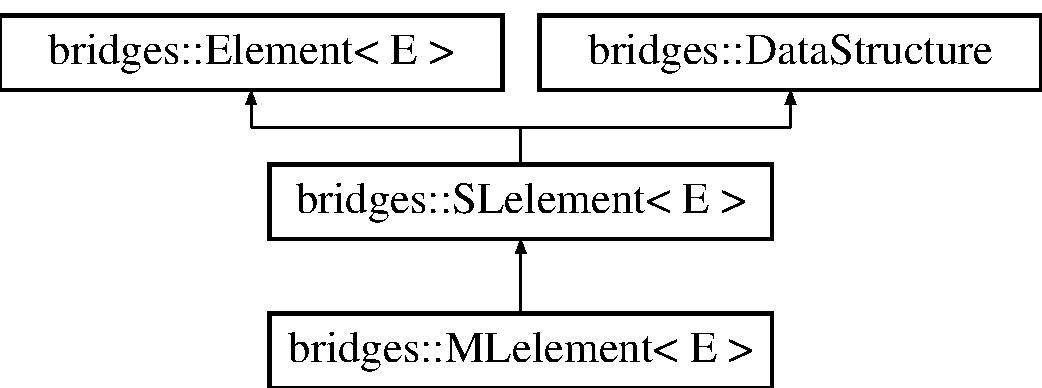
\includegraphics[height=3.000000cm]{classbridges_1_1_m_lelement}
\end{center}
\end{figure}
\subsection*{Public Member Functions}
\begin{DoxyCompactItemize}
\item 
\mbox{\hyperlink{classbridges_1_1_m_lelement_a5d0e64b99abf4d1ad1d2cc89ca28343c}{M\+Lelement}} (const \mbox{\hyperlink{namespacebridges_acfb0a4f7877d8f63de3e6862004c50eda3a3ea00cfc35332cedf6e5e9a32e94da}{E}} \&val=\mbox{\hyperlink{namespacebridges_acfb0a4f7877d8f63de3e6862004c50eda3a3ea00cfc35332cedf6e5e9a32e94da}{E}}(), const string \&lab=string())
\item 
\mbox{\hyperlink{classbridges_1_1_m_lelement_ade42b08d96030f1ed5b92c5613d5cedd}{M\+Lelement}} (string label)
\item 
\mbox{\hyperlink{classbridges_1_1_m_lelement_aaab4924754f94138bb110efd4c047411}{M\+Lelement}} (\mbox{\hyperlink{namespacebridges_acfb0a4f7877d8f63de3e6862004c50eda3a3ea00cfc35332cedf6e5e9a32e94da}{E}} \mbox{\hyperlink{namespacebridges_acfb0a4f7877d8f63de3e6862004c50edae1671797c52e15f763380b45e841ec32}{e}}, \mbox{\hyperlink{classbridges_1_1_m_lelement}{M\+Lelement}}$<$ \mbox{\hyperlink{namespacebridges_acfb0a4f7877d8f63de3e6862004c50eda3a3ea00cfc35332cedf6e5e9a32e94da}{E}} $>$ $\ast$\mbox{\hyperlink{classbridges_1_1_s_lelement_ad7449d10a09ebc52653a7baed812aa43}{next}})
\item 
void \mbox{\hyperlink{classbridges_1_1_m_lelement_ad436f6424e7542ac92df93509f16c7e7}{set\+Sub\+List}} (\mbox{\hyperlink{classbridges_1_1_m_lelement}{M\+Lelement}}$<$ \mbox{\hyperlink{namespacebridges_acfb0a4f7877d8f63de3e6862004c50eda3a3ea00cfc35332cedf6e5e9a32e94da}{E}} $>$ $\ast$sl)
\item 
\mbox{\hyperlink{classbridges_1_1_m_lelement}{M\+Lelement}} $\ast$ \mbox{\hyperlink{classbridges_1_1_m_lelement_a55f82b59284e22caef23959e023614cc}{get\+Sub\+List}} ()
\item 
string \mbox{\hyperlink{classbridges_1_1_m_lelement_a49e5d132e80531f005e1d2da666f0c39}{get\+Data\+Struct\+Type}} ()
\item 
\mbox{\hyperlink{classbridges_1_1_m_lelement}{M\+Lelement}}$<$ \mbox{\hyperlink{namespacebridges_acfb0a4f7877d8f63de3e6862004c50eda3a3ea00cfc35332cedf6e5e9a32e94da}{E}} $>$ $\ast$ \mbox{\hyperlink{classbridges_1_1_m_lelement_aceebd292e7d497f44eea5c4845e7709f}{get\+Next}} () override
\item 
\mbox{\hyperlink{classbridges_1_1_m_lelement}{M\+Lelement}}$<$ \mbox{\hyperlink{namespacebridges_acfb0a4f7877d8f63de3e6862004c50eda3a3ea00cfc35332cedf6e5e9a32e94da}{E}} $>$ $\ast$ \mbox{\hyperlink{classbridges_1_1_m_lelement_aef3e5750e334331597bce94710745d1e}{get\+Next}} () const override
\item 
void \mbox{\hyperlink{classbridges_1_1_m_lelement_aec9747cee60fcafbe474709a9dad21dc}{set\+Next}} (\mbox{\hyperlink{classbridges_1_1_m_lelement}{M\+Lelement}}$<$ \mbox{\hyperlink{namespacebridges_acfb0a4f7877d8f63de3e6862004c50eda3a3ea00cfc35332cedf6e5e9a32e94da}{E}} $>$ $\ast$\mbox{\hyperlink{namespacebridges_acfb0a4f7877d8f63de3e6862004c50eda7b8b965ad4bca0e41ab51de7b31363a1}{n}})
\item 
void \mbox{\hyperlink{classbridges_1_1_m_lelement_a525e43688c15f38382b2d471e1b8d39f}{set\+Tag}} (bool \mbox{\hyperlink{namespacebridges_acfb0a4f7877d8f63de3e6862004c50edae358efa489f58062f10dd7316b65649e}{t}})
\item 
bool \mbox{\hyperlink{classbridges_1_1_m_lelement_a7ac084867fd83d7742f0a305e44e523a}{get\+Tag}} ()
\item 
virtual const string \mbox{\hyperlink{classbridges_1_1_m_lelement_af6e8a50c38e6481ce2c569d0174c564e}{get\+D\+Stype}} () const override
\end{DoxyCompactItemize}
\subsection*{Protected Attributes}
\begin{DoxyCompactItemize}
\item 
\mbox{\hyperlink{classbridges_1_1_m_lelement}{M\+Lelement}}$<$ \mbox{\hyperlink{namespacebridges_acfb0a4f7877d8f63de3e6862004c50eda3a3ea00cfc35332cedf6e5e9a32e94da}{E}} $>$ $\ast$ \mbox{\hyperlink{classbridges_1_1_m_lelement_aa664b4e694c08e5cc31cc9d317dda100}{sub\+\_\+list}} = nullptr
\item 
bool \mbox{\hyperlink{classbridges_1_1_m_lelement_a0285a07355b2bc3d064c30e20aa2fd55}{tag}} = false
\end{DoxyCompactItemize}
\subsection*{Additional Inherited Members}


\subsection{Detailed Description}
\subsubsection*{template$<$typename E$>$\newline
class bridges\+::\+M\+Lelement$<$ E $>$}

\begin{DoxyVerb}@brief This class can be used to instantiate Multi-list Elements.

This class extends SLelement (singly linked list element) to build multi-lists;
\end{DoxyVerb}
 Multilist elements contain a tag that indicates if the element is a sublist or not; If the element points to a sublist, then the sublist field is the beginning of this sublist. If not, the data field contains the user specified data item and list continues (\mbox{\hyperlink{classbridges_1_1_m_lelement_aceebd292e7d497f44eea5c4845e7709f}{get\+Next()}}/set\+Nex()). As in singly linked elements, the next pointer points to the following list element of the list or sublist.

Multi-\/list elements contain a visualizer (\mbox{\hyperlink{classbridges_1_1_element_visualizer}{Element\+Visualizer}}) object for setting visual attributes (color, shape, opacity, size), necessary for displaying them in a web browser.

Elements also have a \mbox{\hyperlink{classbridges_1_1_link_visualizer}{Link\+Visualizer}} object, that is used when they are linked to another element, appropriate for setting link attributes, for instance, between the current element and its next element. In this case, the link in question is that which connects the element to the following elements; a similar logic follows for sublists.

\begin{DoxyAuthor}{Author}
, Kalpathi Subramanian
\end{DoxyAuthor}
\begin{DoxyDate}{Date}
5/24/17
\end{DoxyDate}

\begin{DoxyParams}{Parameters}
{\em $<$\+E$>$} & The generic parameter object that is part of this element, representing either application specific data, or a pointer to a sublist.\\
\hline
\end{DoxyParams}
\begin{DoxySeeAlso}{See also}
Example Tutorial at ~\newline
 ?? 
\end{DoxySeeAlso}


\subsection{Constructor \& Destructor Documentation}
\mbox{\Hypertarget{classbridges_1_1_m_lelement_a5d0e64b99abf4d1ad1d2cc89ca28343c}\label{classbridges_1_1_m_lelement_a5d0e64b99abf4d1ad1d2cc89ca28343c}} 
\index{bridges::MLelement$<$ E $>$@{bridges::MLelement$<$ E $>$}!MLelement@{MLelement}}
\index{MLelement@{MLelement}!bridges::MLelement$<$ E $>$@{bridges::MLelement$<$ E $>$}}
\subsubsection{\texorpdfstring{MLelement()}{MLelement()}\hspace{0.1cm}{\footnotesize\ttfamily [1/3]}}
{\footnotesize\ttfamily template$<$typename E$>$ \\
\mbox{\hyperlink{classbridges_1_1_m_lelement}{bridges\+::\+M\+Lelement}}$<$ \mbox{\hyperlink{namespacebridges_acfb0a4f7877d8f63de3e6862004c50eda3a3ea00cfc35332cedf6e5e9a32e94da}{E}} $>$\+::\mbox{\hyperlink{classbridges_1_1_m_lelement}{M\+Lelement}} (\begin{DoxyParamCaption}\item[{const \mbox{\hyperlink{namespacebridges_acfb0a4f7877d8f63de3e6862004c50eda3a3ea00cfc35332cedf6e5e9a32e94da}{E}} \&}]{val = {\ttfamily \mbox{\hyperlink{namespacebridges_acfb0a4f7877d8f63de3e6862004c50eda3a3ea00cfc35332cedf6e5e9a32e94da}{E}}()},  }\item[{const string \&}]{lab = {\ttfamily string()} }\end{DoxyParamCaption})\hspace{0.3cm}{\ttfamily [inline]}}

This constructor creates an \mbox{\hyperlink{classbridges_1_1_m_lelement}{M\+Lelement}} object and sets the next pointer to null \mbox{\Hypertarget{classbridges_1_1_m_lelement_ade42b08d96030f1ed5b92c5613d5cedd}\label{classbridges_1_1_m_lelement_ade42b08d96030f1ed5b92c5613d5cedd}} 
\index{bridges::MLelement$<$ E $>$@{bridges::MLelement$<$ E $>$}!MLelement@{MLelement}}
\index{MLelement@{MLelement}!bridges::MLelement$<$ E $>$@{bridges::MLelement$<$ E $>$}}
\subsubsection{\texorpdfstring{MLelement()}{MLelement()}\hspace{0.1cm}{\footnotesize\ttfamily [2/3]}}
{\footnotesize\ttfamily template$<$typename E$>$ \\
\mbox{\hyperlink{classbridges_1_1_m_lelement}{bridges\+::\+M\+Lelement}}$<$ \mbox{\hyperlink{namespacebridges_acfb0a4f7877d8f63de3e6862004c50eda3a3ea00cfc35332cedf6e5e9a32e94da}{E}} $>$\+::\mbox{\hyperlink{classbridges_1_1_m_lelement}{M\+Lelement}} (\begin{DoxyParamCaption}\item[{string}]{label }\end{DoxyParamCaption})\hspace{0.3cm}{\ttfamily [inline]}}

This constructor creates an \mbox{\hyperlink{classbridges_1_1_s_lelement}{S\+Lelement}} object of generic parameter object E, and label \char`\"{}label\char`\"{} and sets the next pointer to null


\begin{DoxyParams}{Parameters}
{\em label} & the label of \mbox{\hyperlink{classbridges_1_1_m_lelement}{M\+Lelement}} that shows up on the \mbox{\hyperlink{classbridges_1_1_bridges}{Bridges}} visualization \\
\hline
{\em e} & the generic object that this \mbox{\hyperlink{classbridges_1_1_s_lelement}{S\+Lelement}} will hold \\
\hline
\end{DoxyParams}
\mbox{\Hypertarget{classbridges_1_1_m_lelement_aaab4924754f94138bb110efd4c047411}\label{classbridges_1_1_m_lelement_aaab4924754f94138bb110efd4c047411}} 
\index{bridges::MLelement$<$ E $>$@{bridges::MLelement$<$ E $>$}!MLelement@{MLelement}}
\index{MLelement@{MLelement}!bridges::MLelement$<$ E $>$@{bridges::MLelement$<$ E $>$}}
\subsubsection{\texorpdfstring{MLelement()}{MLelement()}\hspace{0.1cm}{\footnotesize\ttfamily [3/3]}}
{\footnotesize\ttfamily template$<$typename E$>$ \\
\mbox{\hyperlink{classbridges_1_1_m_lelement}{bridges\+::\+M\+Lelement}}$<$ \mbox{\hyperlink{namespacebridges_acfb0a4f7877d8f63de3e6862004c50eda3a3ea00cfc35332cedf6e5e9a32e94da}{E}} $>$\+::\mbox{\hyperlink{classbridges_1_1_m_lelement}{M\+Lelement}} (\begin{DoxyParamCaption}\item[{\mbox{\hyperlink{namespacebridges_acfb0a4f7877d8f63de3e6862004c50eda3a3ea00cfc35332cedf6e5e9a32e94da}{E}}}]{e,  }\item[{\mbox{\hyperlink{classbridges_1_1_m_lelement}{M\+Lelement}}$<$ \mbox{\hyperlink{namespacebridges_acfb0a4f7877d8f63de3e6862004c50eda3a3ea00cfc35332cedf6e5e9a32e94da}{E}} $>$ $\ast$}]{next }\end{DoxyParamCaption})\hspace{0.3cm}{\ttfamily [inline]}}

Creates a new element with value \char`\"{}e\char`\"{} and sets the next pointer to the \mbox{\hyperlink{classbridges_1_1_m_lelement}{M\+Lelement}} referenced by the \char`\"{}next\char`\"{} argument


\begin{DoxyParams}{Parameters}
{\em e} & the generic object that this element will hold \\
\hline
{\em next} & the element that should be assigned to the next pointer \\
\hline
\end{DoxyParams}


\subsection{Member Function Documentation}
\mbox{\Hypertarget{classbridges_1_1_m_lelement_a49e5d132e80531f005e1d2da666f0c39}\label{classbridges_1_1_m_lelement_a49e5d132e80531f005e1d2da666f0c39}} 
\index{bridges::MLelement$<$ E $>$@{bridges::MLelement$<$ E $>$}!getDataStructType@{getDataStructType}}
\index{getDataStructType@{getDataStructType}!bridges::MLelement$<$ E $>$@{bridges::MLelement$<$ E $>$}}
\subsubsection{\texorpdfstring{getDataStructType()}{getDataStructType()}}
{\footnotesize\ttfamily template$<$typename E$>$ \\
string \mbox{\hyperlink{classbridges_1_1_m_lelement}{bridges\+::\+M\+Lelement}}$<$ \mbox{\hyperlink{namespacebridges_acfb0a4f7877d8f63de3e6862004c50eda3a3ea00cfc35332cedf6e5e9a32e94da}{E}} $>$\+::get\+Data\+Struct\+Type (\begin{DoxyParamCaption}{ }\end{DoxyParamCaption})\hspace{0.3cm}{\ttfamily [inline]}}

This method gets the data structure type

\begin{DoxyReturn}{Returns}
The date structure type as a string 
\end{DoxyReturn}
\mbox{\Hypertarget{classbridges_1_1_m_lelement_af6e8a50c38e6481ce2c569d0174c564e}\label{classbridges_1_1_m_lelement_af6e8a50c38e6481ce2c569d0174c564e}} 
\index{bridges::MLelement$<$ E $>$@{bridges::MLelement$<$ E $>$}!getDStype@{getDStype}}
\index{getDStype@{getDStype}!bridges::MLelement$<$ E $>$@{bridges::MLelement$<$ E $>$}}
\subsubsection{\texorpdfstring{getDStype()}{getDStype()}}
{\footnotesize\ttfamily template$<$typename E$>$ \\
virtual const string \mbox{\hyperlink{classbridges_1_1_m_lelement}{bridges\+::\+M\+Lelement}}$<$ \mbox{\hyperlink{namespacebridges_acfb0a4f7877d8f63de3e6862004c50eda3a3ea00cfc35332cedf6e5e9a32e94da}{E}} $>$\+::get\+D\+Stype (\begin{DoxyParamCaption}{ }\end{DoxyParamCaption}) const\hspace{0.3cm}{\ttfamily [inline]}, {\ttfamily [override]}, {\ttfamily [virtual]}}

\begin{DoxyReturn}{Returns}
The string representation of this data structure type 
\end{DoxyReturn}


Reimplemented from \mbox{\hyperlink{classbridges_1_1_s_lelement_a136330b3481a47b3edb429f323274655}{bridges\+::\+S\+Lelement$<$ E $>$}}.

\mbox{\Hypertarget{classbridges_1_1_m_lelement_aceebd292e7d497f44eea5c4845e7709f}\label{classbridges_1_1_m_lelement_aceebd292e7d497f44eea5c4845e7709f}} 
\index{bridges::MLelement$<$ E $>$@{bridges::MLelement$<$ E $>$}!getNext@{getNext}}
\index{getNext@{getNext}!bridges::MLelement$<$ E $>$@{bridges::MLelement$<$ E $>$}}
\subsubsection{\texorpdfstring{getNext()}{getNext()}\hspace{0.1cm}{\footnotesize\ttfamily [1/2]}}
{\footnotesize\ttfamily template$<$typename E$>$ \\
\mbox{\hyperlink{classbridges_1_1_m_lelement}{M\+Lelement}}$<$\mbox{\hyperlink{namespacebridges_acfb0a4f7877d8f63de3e6862004c50eda3a3ea00cfc35332cedf6e5e9a32e94da}{E}}$>$$\ast$ \mbox{\hyperlink{classbridges_1_1_m_lelement}{bridges\+::\+M\+Lelement}}$<$ \mbox{\hyperlink{namespacebridges_acfb0a4f7877d8f63de3e6862004c50eda3a3ea00cfc35332cedf6e5e9a32e94da}{E}} $>$\+::get\+Next (\begin{DoxyParamCaption}{ }\end{DoxyParamCaption})\hspace{0.3cm}{\ttfamily [inline]}, {\ttfamily [override]}, {\ttfamily [virtual]}}

Retrieves the element following this element

\begin{DoxyReturn}{Returns}
M\+Lelement$<$\+E$>$ assigned to next 
\end{DoxyReturn}


Reimplemented from \mbox{\hyperlink{classbridges_1_1_s_lelement_a5bd74108a9aa49339378bf62cdbb19ca}{bridges\+::\+S\+Lelement$<$ E $>$}}.

\mbox{\Hypertarget{classbridges_1_1_m_lelement_aef3e5750e334331597bce94710745d1e}\label{classbridges_1_1_m_lelement_aef3e5750e334331597bce94710745d1e}} 
\index{bridges::MLelement$<$ E $>$@{bridges::MLelement$<$ E $>$}!getNext@{getNext}}
\index{getNext@{getNext}!bridges::MLelement$<$ E $>$@{bridges::MLelement$<$ E $>$}}
\subsubsection{\texorpdfstring{getNext()}{getNext()}\hspace{0.1cm}{\footnotesize\ttfamily [2/2]}}
{\footnotesize\ttfamily template$<$typename E$>$ \\
\mbox{\hyperlink{classbridges_1_1_m_lelement}{M\+Lelement}}$<$\mbox{\hyperlink{namespacebridges_acfb0a4f7877d8f63de3e6862004c50eda3a3ea00cfc35332cedf6e5e9a32e94da}{E}}$>$$\ast$ \mbox{\hyperlink{classbridges_1_1_m_lelement}{bridges\+::\+M\+Lelement}}$<$ \mbox{\hyperlink{namespacebridges_acfb0a4f7877d8f63de3e6862004c50eda3a3ea00cfc35332cedf6e5e9a32e94da}{E}} $>$\+::get\+Next (\begin{DoxyParamCaption}{ }\end{DoxyParamCaption}) const\hspace{0.3cm}{\ttfamily [inline]}, {\ttfamily [override]}, {\ttfamily [virtual]}}

Retrieves the element following this element -\/ const version

\begin{DoxyReturn}{Returns}
M\+Lelement$<$\+E$>$ assigned to next 
\end{DoxyReturn}


Reimplemented from \mbox{\hyperlink{classbridges_1_1_s_lelement_a4422b7731a84734d312b8cd8e241b1e8}{bridges\+::\+S\+Lelement$<$ E $>$}}.

\mbox{\Hypertarget{classbridges_1_1_m_lelement_a55f82b59284e22caef23959e023614cc}\label{classbridges_1_1_m_lelement_a55f82b59284e22caef23959e023614cc}} 
\index{bridges::MLelement$<$ E $>$@{bridges::MLelement$<$ E $>$}!getSubList@{getSubList}}
\index{getSubList@{getSubList}!bridges::MLelement$<$ E $>$@{bridges::MLelement$<$ E $>$}}
\subsubsection{\texorpdfstring{getSubList()}{getSubList()}}
{\footnotesize\ttfamily template$<$typename E$>$ \\
\mbox{\hyperlink{classbridges_1_1_m_lelement}{M\+Lelement}}$\ast$ \mbox{\hyperlink{classbridges_1_1_m_lelement}{bridges\+::\+M\+Lelement}}$<$ \mbox{\hyperlink{namespacebridges_acfb0a4f7877d8f63de3e6862004c50eda3a3ea00cfc35332cedf6e5e9a32e94da}{E}} $>$\+::get\+Sub\+List (\begin{DoxyParamCaption}{ }\end{DoxyParamCaption})\hspace{0.3cm}{\ttfamily [inline]}}

Gets the sublist at this node, if it exists

\begin{DoxyReturn}{Returns}
the sublist head element, if it exists 
\end{DoxyReturn}
\mbox{\Hypertarget{classbridges_1_1_m_lelement_a7ac084867fd83d7742f0a305e44e523a}\label{classbridges_1_1_m_lelement_a7ac084867fd83d7742f0a305e44e523a}} 
\index{bridges::MLelement$<$ E $>$@{bridges::MLelement$<$ E $>$}!getTag@{getTag}}
\index{getTag@{getTag}!bridges::MLelement$<$ E $>$@{bridges::MLelement$<$ E $>$}}
\subsubsection{\texorpdfstring{getTag()}{getTag()}}
{\footnotesize\ttfamily template$<$typename E$>$ \\
bool \mbox{\hyperlink{classbridges_1_1_m_lelement}{bridges\+::\+M\+Lelement}}$<$ \mbox{\hyperlink{namespacebridges_acfb0a4f7877d8f63de3e6862004c50eda3a3ea00cfc35332cedf6e5e9a32e94da}{E}} $>$\+::get\+Tag (\begin{DoxyParamCaption}{ }\end{DoxyParamCaption})\hspace{0.3cm}{\ttfamily [inline]}}

Gets the tag of the element.

\begin{DoxyReturn}{Returns}
tag of the element 
\end{DoxyReturn}
\mbox{\Hypertarget{classbridges_1_1_m_lelement_aec9747cee60fcafbe474709a9dad21dc}\label{classbridges_1_1_m_lelement_aec9747cee60fcafbe474709a9dad21dc}} 
\index{bridges::MLelement$<$ E $>$@{bridges::MLelement$<$ E $>$}!setNext@{setNext}}
\index{setNext@{setNext}!bridges::MLelement$<$ E $>$@{bridges::MLelement$<$ E $>$}}
\subsubsection{\texorpdfstring{setNext()}{setNext()}}
{\footnotesize\ttfamily template$<$typename E$>$ \\
void \mbox{\hyperlink{classbridges_1_1_m_lelement}{bridges\+::\+M\+Lelement}}$<$ \mbox{\hyperlink{namespacebridges_acfb0a4f7877d8f63de3e6862004c50eda3a3ea00cfc35332cedf6e5e9a32e94da}{E}} $>$\+::set\+Next (\begin{DoxyParamCaption}\item[{\mbox{\hyperlink{classbridges_1_1_m_lelement}{M\+Lelement}}$<$ \mbox{\hyperlink{namespacebridges_acfb0a4f7877d8f63de3e6862004c50eda3a3ea00cfc35332cedf6e5e9a32e94da}{E}} $>$ $\ast$}]{n }\end{DoxyParamCaption})\hspace{0.3cm}{\ttfamily [inline]}}

Sets the element to point to the next \mbox{\hyperlink{classbridges_1_1_m_lelement}{M\+Lelement}}


\begin{DoxyParams}{Parameters}
{\em next} & M\+Lelement$<$\+E$>$ that should be assigned to the next pointer \\
\hline
\end{DoxyParams}
\mbox{\Hypertarget{classbridges_1_1_m_lelement_ad436f6424e7542ac92df93509f16c7e7}\label{classbridges_1_1_m_lelement_ad436f6424e7542ac92df93509f16c7e7}} 
\index{bridges::MLelement$<$ E $>$@{bridges::MLelement$<$ E $>$}!setSubList@{setSubList}}
\index{setSubList@{setSubList}!bridges::MLelement$<$ E $>$@{bridges::MLelement$<$ E $>$}}
\subsubsection{\texorpdfstring{setSubList()}{setSubList()}}
{\footnotesize\ttfamily template$<$typename E$>$ \\
void \mbox{\hyperlink{classbridges_1_1_m_lelement}{bridges\+::\+M\+Lelement}}$<$ \mbox{\hyperlink{namespacebridges_acfb0a4f7877d8f63de3e6862004c50eda3a3ea00cfc35332cedf6e5e9a32e94da}{E}} $>$\+::set\+Sub\+List (\begin{DoxyParamCaption}\item[{\mbox{\hyperlink{classbridges_1_1_m_lelement}{M\+Lelement}}$<$ \mbox{\hyperlink{namespacebridges_acfb0a4f7877d8f63de3e6862004c50eda3a3ea00cfc35332cedf6e5e9a32e94da}{E}} $>$ $\ast$}]{sl }\end{DoxyParamCaption})\hspace{0.3cm}{\ttfamily [inline]}}

Sets the start of a new sublist. to the \mbox{\hyperlink{classbridges_1_1_m_lelement}{M\+Lelement}} \char`\"{}next\char`\"{}


\begin{DoxyParams}{Parameters}
{\em sl} & the \mbox{\hyperlink{classbridges_1_1_m_lelement}{M\+Lelement}} that is the beginning of a sublist \\
\hline
\end{DoxyParams}
\mbox{\Hypertarget{classbridges_1_1_m_lelement_a525e43688c15f38382b2d471e1b8d39f}\label{classbridges_1_1_m_lelement_a525e43688c15f38382b2d471e1b8d39f}} 
\index{bridges::MLelement$<$ E $>$@{bridges::MLelement$<$ E $>$}!setTag@{setTag}}
\index{setTag@{setTag}!bridges::MLelement$<$ E $>$@{bridges::MLelement$<$ E $>$}}
\subsubsection{\texorpdfstring{setTag()}{setTag()}}
{\footnotesize\ttfamily template$<$typename E$>$ \\
void \mbox{\hyperlink{classbridges_1_1_m_lelement}{bridges\+::\+M\+Lelement}}$<$ \mbox{\hyperlink{namespacebridges_acfb0a4f7877d8f63de3e6862004c50eda3a3ea00cfc35332cedf6e5e9a32e94da}{E}} $>$\+::set\+Tag (\begin{DoxyParamCaption}\item[{bool}]{t }\end{DoxyParamCaption})\hspace{0.3cm}{\ttfamily [inline]}}

Sets the tag of the element.


\begin{DoxyParams}{Parameters}
{\em boolean} & t \\
\hline
\end{DoxyParams}


\subsection{Member Data Documentation}
\mbox{\Hypertarget{classbridges_1_1_m_lelement_aa664b4e694c08e5cc31cc9d317dda100}\label{classbridges_1_1_m_lelement_aa664b4e694c08e5cc31cc9d317dda100}} 
\index{bridges::MLelement$<$ E $>$@{bridges::MLelement$<$ E $>$}!sub\_list@{sub\_list}}
\index{sub\_list@{sub\_list}!bridges::MLelement$<$ E $>$@{bridges::MLelement$<$ E $>$}}
\subsubsection{\texorpdfstring{sub\_list}{sub\_list}}
{\footnotesize\ttfamily template$<$typename E$>$ \\
\mbox{\hyperlink{classbridges_1_1_m_lelement}{M\+Lelement}}$<$\mbox{\hyperlink{namespacebridges_acfb0a4f7877d8f63de3e6862004c50eda3a3ea00cfc35332cedf6e5e9a32e94da}{E}}$>$$\ast$ \mbox{\hyperlink{classbridges_1_1_m_lelement}{bridges\+::\+M\+Lelement}}$<$ \mbox{\hyperlink{namespacebridges_acfb0a4f7877d8f63de3e6862004c50eda3a3ea00cfc35332cedf6e5e9a32e94da}{E}} $>$\+::sub\+\_\+list = nullptr\hspace{0.3cm}{\ttfamily [protected]}}

\mbox{\Hypertarget{classbridges_1_1_m_lelement_a0285a07355b2bc3d064c30e20aa2fd55}\label{classbridges_1_1_m_lelement_a0285a07355b2bc3d064c30e20aa2fd55}} 
\index{bridges::MLelement$<$ E $>$@{bridges::MLelement$<$ E $>$}!tag@{tag}}
\index{tag@{tag}!bridges::MLelement$<$ E $>$@{bridges::MLelement$<$ E $>$}}
\subsubsection{\texorpdfstring{tag}{tag}}
{\footnotesize\ttfamily template$<$typename E$>$ \\
bool \mbox{\hyperlink{classbridges_1_1_m_lelement}{bridges\+::\+M\+Lelement}}$<$ \mbox{\hyperlink{namespacebridges_acfb0a4f7877d8f63de3e6862004c50eda3a3ea00cfc35332cedf6e5e9a32e94da}{E}} $>$\+::tag = false\hspace{0.3cm}{\ttfamily [protected]}}



The documentation for this class was generated from the following file\+:\begin{DoxyCompactItemize}
\item 
/\+Users/kalpathi/gr/bridges/cxx/src/\mbox{\hyperlink{_m_lelement_8h}{M\+Lelement.\+h}}\end{DoxyCompactItemize}

\hypertarget{classbridges_1_1_server_comm}{}\section{bridges\+:\+:Server\+Comm Class Reference}
\label{classbridges_1_1_server_comm}\index{bridges\+::\+Server\+Comm@{bridges\+::\+Server\+Comm}}


This is a detail class for the \mbox{\hyperlink{classbridges_1_1_bridges}{Bridges}} namespace and is not intended for external use.  




{\ttfamily \#include $<$Server\+Comm.\+h$>$}

\subsection*{Friends}
\begin{DoxyCompactItemize}
\item 
class \mbox{\hyperlink{classbridges_1_1_server_comm_a1e7012f84e4df45aa77f36ad8d8375eb}{Bridges}}
\item 
class \mbox{\hyperlink{classbridges_1_1_server_comm_a7998ddaa8bd7c3b9a7cd2a8cbf3573c4}{Data\+Source}}
\end{DoxyCompactItemize}


\subsection{Detailed Description}
This is a detail class for the \mbox{\hyperlink{classbridges_1_1_bridges}{Bridges}} namespace and is not intended for external use. 

\subsection{Friends And Related Function Documentation}
\mbox{\Hypertarget{classbridges_1_1_server_comm_a1e7012f84e4df45aa77f36ad8d8375eb}\label{classbridges_1_1_server_comm_a1e7012f84e4df45aa77f36ad8d8375eb}} 
\index{bridges\+::\+Server\+Comm@{bridges\+::\+Server\+Comm}!Bridges@{Bridges}}
\index{Bridges@{Bridges}!bridges\+::\+Server\+Comm@{bridges\+::\+Server\+Comm}}
\subsubsection{\texorpdfstring{Bridges}{Bridges}}
{\footnotesize\ttfamily friend class \mbox{\hyperlink{classbridges_1_1_bridges}{Bridges}}\hspace{0.3cm}{\ttfamily [friend]}}

\mbox{\Hypertarget{classbridges_1_1_server_comm_a7998ddaa8bd7c3b9a7cd2a8cbf3573c4}\label{classbridges_1_1_server_comm_a7998ddaa8bd7c3b9a7cd2a8cbf3573c4}} 
\index{bridges\+::\+Server\+Comm@{bridges\+::\+Server\+Comm}!Data\+Source@{Data\+Source}}
\index{Data\+Source@{Data\+Source}!bridges\+::\+Server\+Comm@{bridges\+::\+Server\+Comm}}
\subsubsection{\texorpdfstring{Data\+Source}{DataSource}}
{\footnotesize\ttfamily friend class \mbox{\hyperlink{classbridges_1_1_data_source}{Data\+Source}}\hspace{0.3cm}{\ttfamily [friend]}}



The documentation for this class was generated from the following file\+:\begin{DoxyCompactItemize}
\item 
/\+Users/kalpathi/gr/bridges/client/cxx/bridges18/src/\mbox{\hyperlink{_server_comm_8h}{Server\+Comm.\+h}}\end{DoxyCompactItemize}

\hypertarget{classbridges_1_1_shakespeare}{}\section{bridges\+:\+:Shakespeare Class Reference}
\label{classbridges_1_1_shakespeare}\index{bridges\+::\+Shakespeare@{bridges\+::\+Shakespeare}}


A \hyperlink{classbridges_1_1_shakespeare}{Shakespeare} book object, used along with the \hyperlink{classbridges_1_1_shakespeare}{Shakespeare} books data source.  




{\ttfamily \#include $<$Shakespeare.\+h$>$}

\subsection*{Public Member Functions}
\begin{DoxyCompactItemize}
\item 
\hyperlink{classbridges_1_1_shakespeare_aa1903f3ffb483345c4053c2f315571eb}{Shakespeare} ()
\item 
\hyperlink{classbridges_1_1_shakespeare_a020cc81d13f5c17e362d467d700ac781}{Shakespeare} (string title, string type, string text)
\item 
string \hyperlink{classbridges_1_1_shakespeare_af23ec257146d9a50cf8686dd394ad47b}{get\+Title} () const 
\item 
void \hyperlink{classbridges_1_1_shakespeare_a533ff5a5dd8681ab1156c7345f85ad82}{set\+Title} (string title)
\item 
string \hyperlink{classbridges_1_1_shakespeare_a9bea73dcf0f110601c704c7c22f1f4ab}{get\+Type} () const 
\item 
void \hyperlink{classbridges_1_1_shakespeare_a2bc1ebcfa8b28a590a1f6f83e26ce051}{set\+Type} (string type)
\item 
string \hyperlink{classbridges_1_1_shakespeare_ae9220e3bb7ec01021996542bea34054d}{get\+Text} () const 
\item 
void \hyperlink{classbridges_1_1_shakespeare_a58e8cb2a96ce9af45fcf963694a3aba7}{set\+Text} (string text)
\end{DoxyCompactItemize}


\subsection{Detailed Description}
A \hyperlink{classbridges_1_1_shakespeare}{Shakespeare} book object, used along with the \hyperlink{classbridges_1_1_shakespeare}{Shakespeare} books data source. 

This is a convenience class provided for users who wish to use this data source as part of their application. It provides an A\+P\+I that makes it easy to access the attributes of this data set.

Refer to tutorial examples to using this data source in data structure assignments.

\begin{DoxyAuthor}{Author}
Kalpathi Subramanian 
\end{DoxyAuthor}
\begin{DoxyDate}{Date}
1/16/17 
\end{DoxyDate}


\subsection{Constructor \& Destructor Documentation}
\hypertarget{classbridges_1_1_shakespeare_aa1903f3ffb483345c4053c2f315571eb}{}\index{bridges\+::\+Shakespeare@{bridges\+::\+Shakespeare}!Shakespeare@{Shakespeare}}
\index{Shakespeare@{Shakespeare}!bridges\+::\+Shakespeare@{bridges\+::\+Shakespeare}}
\subsubsection[{Shakespeare()}]{\setlength{\rightskip}{0pt plus 5cm}bridges\+::\+Shakespeare\+::\+Shakespeare (
\begin{DoxyParamCaption}
{}
\end{DoxyParamCaption}
)\hspace{0.3cm}{\ttfamily [inline]}}\label{classbridges_1_1_shakespeare_aa1903f3ffb483345c4053c2f315571eb}
\hypertarget{classbridges_1_1_shakespeare_a020cc81d13f5c17e362d467d700ac781}{}\index{bridges\+::\+Shakespeare@{bridges\+::\+Shakespeare}!Shakespeare@{Shakespeare}}
\index{Shakespeare@{Shakespeare}!bridges\+::\+Shakespeare@{bridges\+::\+Shakespeare}}
\subsubsection[{Shakespeare(string title, string type, string text)}]{\setlength{\rightskip}{0pt plus 5cm}bridges\+::\+Shakespeare\+::\+Shakespeare (
\begin{DoxyParamCaption}
\item[{string}]{title, }
\item[{string}]{type, }
\item[{string}]{text}
\end{DoxyParamCaption}
)\hspace{0.3cm}{\ttfamily [inline]}}\label{classbridges_1_1_shakespeare_a020cc81d13f5c17e362d467d700ac781}


\subsection{Member Function Documentation}
\hypertarget{classbridges_1_1_shakespeare_ae9220e3bb7ec01021996542bea34054d}{}\index{bridges\+::\+Shakespeare@{bridges\+::\+Shakespeare}!get\+Text@{get\+Text}}
\index{get\+Text@{get\+Text}!bridges\+::\+Shakespeare@{bridges\+::\+Shakespeare}}
\subsubsection[{get\+Text() const }]{\setlength{\rightskip}{0pt plus 5cm}string bridges\+::\+Shakespeare\+::get\+Text (
\begin{DoxyParamCaption}
{}
\end{DoxyParamCaption}
) const\hspace{0.3cm}{\ttfamily [inline]}}\label{classbridges_1_1_shakespeare_ae9220e3bb7ec01021996542bea34054d}
\hypertarget{classbridges_1_1_shakespeare_af23ec257146d9a50cf8686dd394ad47b}{}\index{bridges\+::\+Shakespeare@{bridges\+::\+Shakespeare}!get\+Title@{get\+Title}}
\index{get\+Title@{get\+Title}!bridges\+::\+Shakespeare@{bridges\+::\+Shakespeare}}
\subsubsection[{get\+Title() const }]{\setlength{\rightskip}{0pt plus 5cm}string bridges\+::\+Shakespeare\+::get\+Title (
\begin{DoxyParamCaption}
{}
\end{DoxyParamCaption}
) const\hspace{0.3cm}{\ttfamily [inline]}}\label{classbridges_1_1_shakespeare_af23ec257146d9a50cf8686dd394ad47b}
\hypertarget{classbridges_1_1_shakespeare_a9bea73dcf0f110601c704c7c22f1f4ab}{}\index{bridges\+::\+Shakespeare@{bridges\+::\+Shakespeare}!get\+Type@{get\+Type}}
\index{get\+Type@{get\+Type}!bridges\+::\+Shakespeare@{bridges\+::\+Shakespeare}}
\subsubsection[{get\+Type() const }]{\setlength{\rightskip}{0pt plus 5cm}string bridges\+::\+Shakespeare\+::get\+Type (
\begin{DoxyParamCaption}
{}
\end{DoxyParamCaption}
) const\hspace{0.3cm}{\ttfamily [inline]}}\label{classbridges_1_1_shakespeare_a9bea73dcf0f110601c704c7c22f1f4ab}
\hypertarget{classbridges_1_1_shakespeare_a58e8cb2a96ce9af45fcf963694a3aba7}{}\index{bridges\+::\+Shakespeare@{bridges\+::\+Shakespeare}!set\+Text@{set\+Text}}
\index{set\+Text@{set\+Text}!bridges\+::\+Shakespeare@{bridges\+::\+Shakespeare}}
\subsubsection[{set\+Text(string text)}]{\setlength{\rightskip}{0pt plus 5cm}void bridges\+::\+Shakespeare\+::set\+Text (
\begin{DoxyParamCaption}
\item[{string}]{text}
\end{DoxyParamCaption}
)\hspace{0.3cm}{\ttfamily [inline]}}\label{classbridges_1_1_shakespeare_a58e8cb2a96ce9af45fcf963694a3aba7}
\hypertarget{classbridges_1_1_shakespeare_a533ff5a5dd8681ab1156c7345f85ad82}{}\index{bridges\+::\+Shakespeare@{bridges\+::\+Shakespeare}!set\+Title@{set\+Title}}
\index{set\+Title@{set\+Title}!bridges\+::\+Shakespeare@{bridges\+::\+Shakespeare}}
\subsubsection[{set\+Title(string title)}]{\setlength{\rightskip}{0pt plus 5cm}void bridges\+::\+Shakespeare\+::set\+Title (
\begin{DoxyParamCaption}
\item[{string}]{title}
\end{DoxyParamCaption}
)\hspace{0.3cm}{\ttfamily [inline]}}\label{classbridges_1_1_shakespeare_a533ff5a5dd8681ab1156c7345f85ad82}
\hypertarget{classbridges_1_1_shakespeare_a2bc1ebcfa8b28a590a1f6f83e26ce051}{}\index{bridges\+::\+Shakespeare@{bridges\+::\+Shakespeare}!set\+Type@{set\+Type}}
\index{set\+Type@{set\+Type}!bridges\+::\+Shakespeare@{bridges\+::\+Shakespeare}}
\subsubsection[{set\+Type(string type)}]{\setlength{\rightskip}{0pt plus 5cm}void bridges\+::\+Shakespeare\+::set\+Type (
\begin{DoxyParamCaption}
\item[{string}]{type}
\end{DoxyParamCaption}
)\hspace{0.3cm}{\ttfamily [inline]}}\label{classbridges_1_1_shakespeare_a2bc1ebcfa8b28a590a1f6f83e26ce051}


The documentation for this class was generated from the following file\+:\begin{DoxyCompactItemize}
\item 
/\+Users/krs/gr/bridges/bridges17/cxx/src/data\+\_\+src/\hyperlink{_shakespeare_8h}{Shakespeare.\+h}\end{DoxyCompactItemize}

\hypertarget{classbridges_1_1_s_lelement}{}\section{bridges\+:\+:S\+Lelement$<$ E $>$ Class Template Reference}
\label{classbridges_1_1_s_lelement}\index{bridges\+::\+S\+Lelement$<$ E $>$@{bridges\+::\+S\+Lelement$<$ E $>$}}


The singly linked list element, derived from \hyperlink{classbridges_1_1_element}{Element}.  




{\ttfamily \#include $<$S\+Lelement.\+h$>$}

Inheritance diagram for bridges\+:\+:S\+Lelement$<$ E $>$\+:\begin{figure}[H]
\begin{center}
\leavevmode
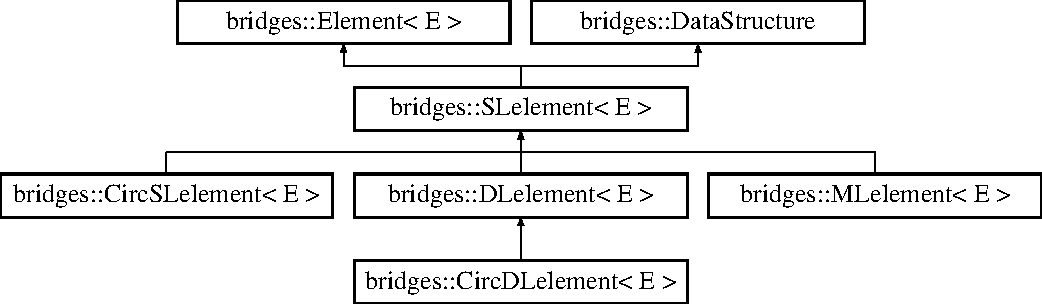
\includegraphics[height=4.000000cm]{classbridges_1_1_s_lelement}
\end{center}
\end{figure}
\subsection*{Public Member Functions}
\begin{DoxyCompactItemize}
\item 
\hyperlink{classbridges_1_1_s_lelement_a9ddac46a935b85cde76305135d16de0a}{S\+Lelement} (\hyperlink{classbridges_1_1_s_lelement}{S\+Lelement} $\ast$n, const E \&val=E(), const string \&lab=string())
\item 
\hyperlink{classbridges_1_1_s_lelement_a76423021747b1f2090847c418c13352b}{S\+Lelement} (const E \&val=E(), const string \&lab=string())
\item 
virtual const string \hyperlink{classbridges_1_1_s_lelement_a136330b3481a47b3edb429f323274655}{get\+D\+Stype} () const override
\item 
virtual \hyperlink{classbridges_1_1_s_lelement}{S\+Lelement} $\ast$ \hyperlink{classbridges_1_1_s_lelement_a5bd74108a9aa49339378bf62cdbb19ca}{get\+Next} ()
\item 
virtual const \hyperlink{classbridges_1_1_s_lelement}{S\+Lelement} $\ast$ \hyperlink{classbridges_1_1_s_lelement_a4422b7731a84734d312b8cd8e241b1e8}{get\+Next} () const
\item 
void \hyperlink{classbridges_1_1_s_lelement_a347f8809406f930ce83bf44764a4f1b5}{set\+Next} (\hyperlink{classbridges_1_1_s_lelement}{S\+Lelement} $\ast$n)
\item 
virtual void \hyperlink{classbridges_1_1_s_lelement_ac747648849874407e9d907bb4557dd52}{cleanup} () override
\end{DoxyCompactItemize}
\subsection*{Protected Attributes}
\begin{DoxyCompactItemize}
\item 
\hyperlink{classbridges_1_1_s_lelement}{S\+Lelement} $\ast$ \hyperlink{classbridges_1_1_s_lelement_ad7449d10a09ebc52653a7baed812aa43}{next} = nullptr
\end{DoxyCompactItemize}
\subsection*{Additional Inherited Members}


\subsection{Detailed Description}
\subsubsection*{template$<$typename E$>$\newline
class bridges\+::\+S\+Lelement$<$ E $>$}

The singly linked list element, derived from \hyperlink{classbridges_1_1_element}{Element}. 

This class can be used to create singly linked elements, with a next \hyperlink{classbridges_1_1_s_lelement}{S\+Lelement} pointer

Generic Parameters\+: E the application data type

\begin{DoxyAuthor}{Author}
Kalpathi Subramanian 
\end{DoxyAuthor}
\begin{DoxyDate}{Date}
6/11/15 
\end{DoxyDate}


\subsection{Constructor \& Destructor Documentation}
\hypertarget{classbridges_1_1_s_lelement_a9ddac46a935b85cde76305135d16de0a}{}\label{classbridges_1_1_s_lelement_a9ddac46a935b85cde76305135d16de0a} 
\index{bridges\+::\+S\+Lelement@{bridges\+::\+S\+Lelement}!S\+Lelement@{S\+Lelement}}
\index{S\+Lelement@{S\+Lelement}!bridges\+::\+S\+Lelement@{bridges\+::\+S\+Lelement}}
\subsubsection{\texorpdfstring{S\+Lelement()}{SLelement()}\hspace{0.1cm}{\footnotesize\ttfamily [1/2]}}
{\footnotesize\ttfamily template$<$typename E$>$ \\
\hyperlink{classbridges_1_1_s_lelement}{bridges\+::\+S\+Lelement}$<$ E $>$\+::\hyperlink{classbridges_1_1_s_lelement}{S\+Lelement} (\begin{DoxyParamCaption}\item[{\hyperlink{classbridges_1_1_s_lelement}{S\+Lelement}$<$ E $>$ $\ast$}]{n,  }\item[{const E \&}]{val = {\ttfamily E()},  }\item[{const string \&}]{lab = {\ttfamily string()} }\end{DoxyParamCaption})\hspace{0.3cm}{\ttfamily [inline]}}

Constructs an slelement with the provided value, label, and next slelement. The defaults will be used if not provided.


\begin{DoxyParams}{Parameters}
{\em val} & The data to hold \\
\hline
{\em lab} & The label to show \\
\hline
{\em n} & The next \hyperlink{classbridges_1_1_s_lelement}{S\+Lelement} \\
\hline
\end{DoxyParams}
\hypertarget{classbridges_1_1_s_lelement_a76423021747b1f2090847c418c13352b}{}\label{classbridges_1_1_s_lelement_a76423021747b1f2090847c418c13352b} 
\index{bridges\+::\+S\+Lelement@{bridges\+::\+S\+Lelement}!S\+Lelement@{S\+Lelement}}
\index{S\+Lelement@{S\+Lelement}!bridges\+::\+S\+Lelement@{bridges\+::\+S\+Lelement}}
\subsubsection{\texorpdfstring{S\+Lelement()}{SLelement()}\hspace{0.1cm}{\footnotesize\ttfamily [2/2]}}
{\footnotesize\ttfamily template$<$typename E$>$ \\
\hyperlink{classbridges_1_1_s_lelement}{bridges\+::\+S\+Lelement}$<$ E $>$\+::\hyperlink{classbridges_1_1_s_lelement}{S\+Lelement} (\begin{DoxyParamCaption}\item[{const E \&}]{val = {\ttfamily E()},  }\item[{const string \&}]{lab = {\ttfamily string()} }\end{DoxyParamCaption})\hspace{0.3cm}{\ttfamily [inline]}}

Constructs an slelement with the provided value and label, setting the next slelement to N\+U\+LL. The defaults will be used if not provided.


\begin{DoxyParams}{Parameters}
{\em val} & The data to hold \\
\hline
{\em lab} & The label to show \\
\hline
\end{DoxyParams}


\subsection{Member Function Documentation}
\hypertarget{classbridges_1_1_s_lelement_ac747648849874407e9d907bb4557dd52}{}\label{classbridges_1_1_s_lelement_ac747648849874407e9d907bb4557dd52} 
\index{bridges\+::\+S\+Lelement@{bridges\+::\+S\+Lelement}!cleanup@{cleanup}}
\index{cleanup@{cleanup}!bridges\+::\+S\+Lelement@{bridges\+::\+S\+Lelement}}
\subsubsection{\texorpdfstring{cleanup()}{cleanup()}}
{\footnotesize\ttfamily template$<$typename E$>$ \\
virtual void \hyperlink{classbridges_1_1_s_lelement}{bridges\+::\+S\+Lelement}$<$ E $>$\+::cleanup (\begin{DoxyParamCaption}{ }\end{DoxyParamCaption})\hspace{0.3cm}{\ttfamily [inline]}, {\ttfamily [override]}, {\ttfamily [virtual]}}

Calls delete on itself and each next linked S\+Lelement$\ast$

\begin{DoxyWarning}{Warning}
Only call if these S\+Lelements were all dynamicaly allocated(aka\+: using new) 

If linked list contains redundant links, delete will be called multiple times on it, leading to undefined behavior 
\end{DoxyWarning}


Reimplemented from \hyperlink{classbridges_1_1_data_structure_ac3ad75810fd77f0ad35b9b5123d2c8f8}{bridges\+::\+Data\+Structure}.

\hypertarget{classbridges_1_1_s_lelement_a136330b3481a47b3edb429f323274655}{}\label{classbridges_1_1_s_lelement_a136330b3481a47b3edb429f323274655} 
\index{bridges\+::\+S\+Lelement@{bridges\+::\+S\+Lelement}!get\+D\+Stype@{get\+D\+Stype}}
\index{get\+D\+Stype@{get\+D\+Stype}!bridges\+::\+S\+Lelement@{bridges\+::\+S\+Lelement}}
\subsubsection{\texorpdfstring{get\+D\+Stype()}{getDStype()}}
{\footnotesize\ttfamily template$<$typename E$>$ \\
virtual const string \hyperlink{classbridges_1_1_s_lelement}{bridges\+::\+S\+Lelement}$<$ E $>$\+::get\+D\+Stype (\begin{DoxyParamCaption}{ }\end{DoxyParamCaption}) const\hspace{0.3cm}{\ttfamily [inline]}, {\ttfamily [override]}, {\ttfamily [virtual]}}

\begin{DoxyReturn}{Returns}
The string representation of this data structure type 
\end{DoxyReturn}


Implements \hyperlink{classbridges_1_1_data_structure_a957a63b106e340bc753620c650632bdc}{bridges\+::\+Data\+Structure}.



Reimplemented in \hyperlink{classbridges_1_1_d_lelement_a109be7aba8bd3d0450859938b5d3144c}{bridges\+::\+D\+Lelement$<$ E $>$}.

\hypertarget{classbridges_1_1_s_lelement_a5bd74108a9aa49339378bf62cdbb19ca}{}\label{classbridges_1_1_s_lelement_a5bd74108a9aa49339378bf62cdbb19ca} 
\index{bridges\+::\+S\+Lelement@{bridges\+::\+S\+Lelement}!get\+Next@{get\+Next}}
\index{get\+Next@{get\+Next}!bridges\+::\+S\+Lelement@{bridges\+::\+S\+Lelement}}
\subsubsection{\texorpdfstring{get\+Next()}{getNext()}\hspace{0.1cm}{\footnotesize\ttfamily [1/2]}}
{\footnotesize\ttfamily template$<$typename E$>$ \\
virtual \hyperlink{classbridges_1_1_s_lelement}{S\+Lelement}$\ast$ \hyperlink{classbridges_1_1_s_lelement}{bridges\+::\+S\+Lelement}$<$ E $>$\+::get\+Next (\begin{DoxyParamCaption}{ }\end{DoxyParamCaption})\hspace{0.3cm}{\ttfamily [inline]}, {\ttfamily [virtual]}}

\begin{DoxyReturn}{Returns}
The next \hyperlink{classbridges_1_1_s_lelement}{S\+Lelement} 
\end{DoxyReturn}


Reimplemented in \hyperlink{classbridges_1_1_circ_s_lelement_aab863627c125c6f1075af7e7b7f340cf}{bridges\+::\+Circ\+S\+Lelement$<$ E $>$}, and \hyperlink{classbridges_1_1_d_lelement_a0c713707d8c7d0a97fe4194ed6592ede}{bridges\+::\+D\+Lelement$<$ E $>$}.

\hypertarget{classbridges_1_1_s_lelement_a4422b7731a84734d312b8cd8e241b1e8}{}\label{classbridges_1_1_s_lelement_a4422b7731a84734d312b8cd8e241b1e8} 
\index{bridges\+::\+S\+Lelement@{bridges\+::\+S\+Lelement}!get\+Next@{get\+Next}}
\index{get\+Next@{get\+Next}!bridges\+::\+S\+Lelement@{bridges\+::\+S\+Lelement}}
\subsubsection{\texorpdfstring{get\+Next()}{getNext()}\hspace{0.1cm}{\footnotesize\ttfamily [2/2]}}
{\footnotesize\ttfamily template$<$typename E$>$ \\
virtual const \hyperlink{classbridges_1_1_s_lelement}{S\+Lelement}$\ast$ \hyperlink{classbridges_1_1_s_lelement}{bridges\+::\+S\+Lelement}$<$ E $>$\+::get\+Next (\begin{DoxyParamCaption}{ }\end{DoxyParamCaption}) const\hspace{0.3cm}{\ttfamily [inline]}, {\ttfamily [virtual]}}

Constant version 

Reimplemented in \hyperlink{classbridges_1_1_circ_d_lelement_ad02db972b2a525de01855bfed1a45ea4}{bridges\+::\+Circ\+D\+Lelement$<$ E $>$}, and \hyperlink{classbridges_1_1_d_lelement_a648012849263b4b1cd2d504d5e5fd880}{bridges\+::\+D\+Lelement$<$ E $>$}.

\hypertarget{classbridges_1_1_s_lelement_a347f8809406f930ce83bf44764a4f1b5}{}\label{classbridges_1_1_s_lelement_a347f8809406f930ce83bf44764a4f1b5} 
\index{bridges\+::\+S\+Lelement@{bridges\+::\+S\+Lelement}!set\+Next@{set\+Next}}
\index{set\+Next@{set\+Next}!bridges\+::\+S\+Lelement@{bridges\+::\+S\+Lelement}}
\subsubsection{\texorpdfstring{set\+Next()}{setNext()}}
{\footnotesize\ttfamily template$<$typename E$>$ \\
void \hyperlink{classbridges_1_1_s_lelement}{bridges\+::\+S\+Lelement}$<$ E $>$\+::set\+Next (\begin{DoxyParamCaption}\item[{\hyperlink{classbridges_1_1_s_lelement}{S\+Lelement}$<$ E $>$ $\ast$}]{n }\end{DoxyParamCaption})\hspace{0.3cm}{\ttfamily [inline]}}

Sets next link to \char`\"{}n\char`\"{}


\begin{DoxyParams}{Parameters}
{\em n} & The next \hyperlink{classbridges_1_1_s_lelement}{S\+Lelement} \\
\hline
\end{DoxyParams}


\subsection{Member Data Documentation}
\hypertarget{classbridges_1_1_s_lelement_ad7449d10a09ebc52653a7baed812aa43}{}\label{classbridges_1_1_s_lelement_ad7449d10a09ebc52653a7baed812aa43} 
\index{bridges\+::\+S\+Lelement@{bridges\+::\+S\+Lelement}!next@{next}}
\index{next@{next}!bridges\+::\+S\+Lelement@{bridges\+::\+S\+Lelement}}
\subsubsection{\texorpdfstring{next}{next}}
{\footnotesize\ttfamily template$<$typename E$>$ \\
\hyperlink{classbridges_1_1_s_lelement}{S\+Lelement}$\ast$ \hyperlink{classbridges_1_1_s_lelement}{bridges\+::\+S\+Lelement}$<$ E $>$\+::next = nullptr\hspace{0.3cm}{\ttfamily [protected]}}



The documentation for this class was generated from the following file\+:\begin{DoxyCompactItemize}
\item 
/\+Users/kalpathi/gr/bridges/client/cxx/git-\/cxx/src/\hyperlink{_s_lelement_8h}{S\+Lelement.\+h}\end{DoxyCompactItemize}

\hypertarget{classbridges_1_1_song}{}\section{bridges\+:\+:Song Class Reference}
\label{classbridges_1_1_song}\index{bridges\+::\+Song@{bridges\+::\+Song}}


{\ttfamily \#include $<$Song.\+h$>$}

\subsection*{Public Member Functions}
\begin{DoxyCompactItemize}
\item 
\mbox{\hyperlink{classbridges_1_1_song_aa938ae0bd6d566d6e2a6bf30beeb0ea5}{Song}} ()
\item 
\mbox{\hyperlink{classbridges_1_1_song_a6bba7d1a1ce20a34b30cfa1cd874faa0}{Song}} (const string \&artist, const string \&song, const string \&album, const string \&lyrics, const string \&release\+\_\+date)
\item 
string \mbox{\hyperlink{classbridges_1_1_song_a22175397f3ca65470d4c7081a3d37a13}{get\+Artist}} () const
\item 
void \mbox{\hyperlink{classbridges_1_1_song_a21569a1b94eced89eed1a2ab8b2ff1ca}{set\+Artist}} (const string \&artist)
\item 
string \mbox{\hyperlink{classbridges_1_1_song_a28eee6f38acce73615a4ff6317a435d4}{get\+Song\+Title}} () const
\item 
void \mbox{\hyperlink{classbridges_1_1_song_a18e3a6bd5f424a6dadf529bed446a0d0}{set\+Song\+Title}} (const string \&song)
\item 
string \mbox{\hyperlink{classbridges_1_1_song_a1e85190c97eb8d2f9ce37dfbdb9f399b}{get\+Album\+Title}} () const
\item 
void \mbox{\hyperlink{classbridges_1_1_song_af89d78b799b672282a60c337327d9988}{set\+Album\+Title}} (const string \&album)
\item 
string \mbox{\hyperlink{classbridges_1_1_song_a54a6ce44a8b553527ba7cb0f8521fb7f}{get\+Lyrics}} () const
\item 
void \mbox{\hyperlink{classbridges_1_1_song_af32f02057c6dd253ea4e8d002e548cf2}{set\+Lyrics}} (const string \&lyrics)
\item 
string \mbox{\hyperlink{classbridges_1_1_song_a0504614f584d42624888caf74cf45060}{get\+Release\+Date}} () const
\item 
void \mbox{\hyperlink{classbridges_1_1_song_a492a14035331c66652488c4f222aa7b3}{set\+Release\+Date}} (const string \&release\+\_\+date)
\end{DoxyCompactItemize}


\subsection{Constructor \& Destructor Documentation}
\mbox{\Hypertarget{classbridges_1_1_song_aa938ae0bd6d566d6e2a6bf30beeb0ea5}\label{classbridges_1_1_song_aa938ae0bd6d566d6e2a6bf30beeb0ea5}} 
\index{bridges\+::\+Song@{bridges\+::\+Song}!Song@{Song}}
\index{Song@{Song}!bridges\+::\+Song@{bridges\+::\+Song}}
\subsubsection{\texorpdfstring{Song()}{Song()}\hspace{0.1cm}{\footnotesize\ttfamily [1/2]}}
{\footnotesize\ttfamily bridges\+::\+Song\+::\+Song (\begin{DoxyParamCaption}{ }\end{DoxyParamCaption})\hspace{0.3cm}{\ttfamily [inline]}}

\mbox{\Hypertarget{classbridges_1_1_song_a6bba7d1a1ce20a34b30cfa1cd874faa0}\label{classbridges_1_1_song_a6bba7d1a1ce20a34b30cfa1cd874faa0}} 
\index{bridges\+::\+Song@{bridges\+::\+Song}!Song@{Song}}
\index{Song@{Song}!bridges\+::\+Song@{bridges\+::\+Song}}
\subsubsection{\texorpdfstring{Song()}{Song()}\hspace{0.1cm}{\footnotesize\ttfamily [2/2]}}
{\footnotesize\ttfamily bridges\+::\+Song\+::\+Song (\begin{DoxyParamCaption}\item[{const string \&}]{artist,  }\item[{const string \&}]{song,  }\item[{const string \&}]{album,  }\item[{const string \&}]{lyrics,  }\item[{const string \&}]{release\+\_\+date }\end{DoxyParamCaption})\hspace{0.3cm}{\ttfamily [inline]}}



\subsection{Member Function Documentation}
\mbox{\Hypertarget{classbridges_1_1_song_a1e85190c97eb8d2f9ce37dfbdb9f399b}\label{classbridges_1_1_song_a1e85190c97eb8d2f9ce37dfbdb9f399b}} 
\index{bridges\+::\+Song@{bridges\+::\+Song}!get\+Album\+Title@{get\+Album\+Title}}
\index{get\+Album\+Title@{get\+Album\+Title}!bridges\+::\+Song@{bridges\+::\+Song}}
\subsubsection{\texorpdfstring{get\+Album\+Title()}{getAlbumTitle()}}
{\footnotesize\ttfamily string bridges\+::\+Song\+::get\+Album\+Title (\begin{DoxyParamCaption}{ }\end{DoxyParamCaption}) const\hspace{0.3cm}{\ttfamily [inline]}}

\mbox{\Hypertarget{classbridges_1_1_song_a22175397f3ca65470d4c7081a3d37a13}\label{classbridges_1_1_song_a22175397f3ca65470d4c7081a3d37a13}} 
\index{bridges\+::\+Song@{bridges\+::\+Song}!get\+Artist@{get\+Artist}}
\index{get\+Artist@{get\+Artist}!bridges\+::\+Song@{bridges\+::\+Song}}
\subsubsection{\texorpdfstring{get\+Artist()}{getArtist()}}
{\footnotesize\ttfamily string bridges\+::\+Song\+::get\+Artist (\begin{DoxyParamCaption}{ }\end{DoxyParamCaption}) const\hspace{0.3cm}{\ttfamily [inline]}}

\mbox{\Hypertarget{classbridges_1_1_song_a54a6ce44a8b553527ba7cb0f8521fb7f}\label{classbridges_1_1_song_a54a6ce44a8b553527ba7cb0f8521fb7f}} 
\index{bridges\+::\+Song@{bridges\+::\+Song}!get\+Lyrics@{get\+Lyrics}}
\index{get\+Lyrics@{get\+Lyrics}!bridges\+::\+Song@{bridges\+::\+Song}}
\subsubsection{\texorpdfstring{get\+Lyrics()}{getLyrics()}}
{\footnotesize\ttfamily string bridges\+::\+Song\+::get\+Lyrics (\begin{DoxyParamCaption}{ }\end{DoxyParamCaption}) const\hspace{0.3cm}{\ttfamily [inline]}}

\mbox{\Hypertarget{classbridges_1_1_song_a0504614f584d42624888caf74cf45060}\label{classbridges_1_1_song_a0504614f584d42624888caf74cf45060}} 
\index{bridges\+::\+Song@{bridges\+::\+Song}!get\+Release\+Date@{get\+Release\+Date}}
\index{get\+Release\+Date@{get\+Release\+Date}!bridges\+::\+Song@{bridges\+::\+Song}}
\subsubsection{\texorpdfstring{get\+Release\+Date()}{getReleaseDate()}}
{\footnotesize\ttfamily string bridges\+::\+Song\+::get\+Release\+Date (\begin{DoxyParamCaption}{ }\end{DoxyParamCaption}) const\hspace{0.3cm}{\ttfamily [inline]}}

\mbox{\Hypertarget{classbridges_1_1_song_a28eee6f38acce73615a4ff6317a435d4}\label{classbridges_1_1_song_a28eee6f38acce73615a4ff6317a435d4}} 
\index{bridges\+::\+Song@{bridges\+::\+Song}!get\+Song\+Title@{get\+Song\+Title}}
\index{get\+Song\+Title@{get\+Song\+Title}!bridges\+::\+Song@{bridges\+::\+Song}}
\subsubsection{\texorpdfstring{get\+Song\+Title()}{getSongTitle()}}
{\footnotesize\ttfamily string bridges\+::\+Song\+::get\+Song\+Title (\begin{DoxyParamCaption}{ }\end{DoxyParamCaption}) const\hspace{0.3cm}{\ttfamily [inline]}}

\mbox{\Hypertarget{classbridges_1_1_song_af89d78b799b672282a60c337327d9988}\label{classbridges_1_1_song_af89d78b799b672282a60c337327d9988}} 
\index{bridges\+::\+Song@{bridges\+::\+Song}!set\+Album\+Title@{set\+Album\+Title}}
\index{set\+Album\+Title@{set\+Album\+Title}!bridges\+::\+Song@{bridges\+::\+Song}}
\subsubsection{\texorpdfstring{set\+Album\+Title()}{setAlbumTitle()}}
{\footnotesize\ttfamily void bridges\+::\+Song\+::set\+Album\+Title (\begin{DoxyParamCaption}\item[{const string \&}]{album }\end{DoxyParamCaption})\hspace{0.3cm}{\ttfamily [inline]}}

\mbox{\Hypertarget{classbridges_1_1_song_a21569a1b94eced89eed1a2ab8b2ff1ca}\label{classbridges_1_1_song_a21569a1b94eced89eed1a2ab8b2ff1ca}} 
\index{bridges\+::\+Song@{bridges\+::\+Song}!set\+Artist@{set\+Artist}}
\index{set\+Artist@{set\+Artist}!bridges\+::\+Song@{bridges\+::\+Song}}
\subsubsection{\texorpdfstring{set\+Artist()}{setArtist()}}
{\footnotesize\ttfamily void bridges\+::\+Song\+::set\+Artist (\begin{DoxyParamCaption}\item[{const string \&}]{artist }\end{DoxyParamCaption})\hspace{0.3cm}{\ttfamily [inline]}}

\mbox{\Hypertarget{classbridges_1_1_song_af32f02057c6dd253ea4e8d002e548cf2}\label{classbridges_1_1_song_af32f02057c6dd253ea4e8d002e548cf2}} 
\index{bridges\+::\+Song@{bridges\+::\+Song}!set\+Lyrics@{set\+Lyrics}}
\index{set\+Lyrics@{set\+Lyrics}!bridges\+::\+Song@{bridges\+::\+Song}}
\subsubsection{\texorpdfstring{set\+Lyrics()}{setLyrics()}}
{\footnotesize\ttfamily void bridges\+::\+Song\+::set\+Lyrics (\begin{DoxyParamCaption}\item[{const string \&}]{lyrics }\end{DoxyParamCaption})\hspace{0.3cm}{\ttfamily [inline]}}

\mbox{\Hypertarget{classbridges_1_1_song_a492a14035331c66652488c4f222aa7b3}\label{classbridges_1_1_song_a492a14035331c66652488c4f222aa7b3}} 
\index{bridges\+::\+Song@{bridges\+::\+Song}!set\+Release\+Date@{set\+Release\+Date}}
\index{set\+Release\+Date@{set\+Release\+Date}!bridges\+::\+Song@{bridges\+::\+Song}}
\subsubsection{\texorpdfstring{set\+Release\+Date()}{setReleaseDate()}}
{\footnotesize\ttfamily void bridges\+::\+Song\+::set\+Release\+Date (\begin{DoxyParamCaption}\item[{const string \&}]{release\+\_\+date }\end{DoxyParamCaption})\hspace{0.3cm}{\ttfamily [inline]}}

\mbox{\Hypertarget{classbridges_1_1_song_a18e3a6bd5f424a6dadf529bed446a0d0}\label{classbridges_1_1_song_a18e3a6bd5f424a6dadf529bed446a0d0}} 
\index{bridges\+::\+Song@{bridges\+::\+Song}!set\+Song\+Title@{set\+Song\+Title}}
\index{set\+Song\+Title@{set\+Song\+Title}!bridges\+::\+Song@{bridges\+::\+Song}}
\subsubsection{\texorpdfstring{set\+Song\+Title()}{setSongTitle()}}
{\footnotesize\ttfamily void bridges\+::\+Song\+::set\+Song\+Title (\begin{DoxyParamCaption}\item[{const string \&}]{song }\end{DoxyParamCaption})\hspace{0.3cm}{\ttfamily [inline]}}



The documentation for this class was generated from the following file\+:\begin{DoxyCompactItemize}
\item 
/\+Users/kalpathi/gr/bridges/client/cxx/bridges18/src/data\+\_\+src/\mbox{\hyperlink{_song_8h}{Song.\+h}}\end{DoxyCompactItemize}

\hypertarget{classbridges_1_1_tree_element}{}\section{bridges\+:\+:Tree\+Element$<$ E $>$ Class Template Reference}
\label{classbridges_1_1_tree_element}\index{bridges\+::\+Tree\+Element$<$ E $>$@{bridges\+::\+Tree\+Element$<$ E $>$}}


This class can be used to create tree elements, derived from \hyperlink{classbridges_1_1_element}{Element}.  




{\ttfamily \#include $<$Tree\+Element.\+h$>$}

Inheritance diagram for bridges\+:\+:Tree\+Element$<$ E $>$\+:\begin{figure}[H]
\begin{center}
\leavevmode
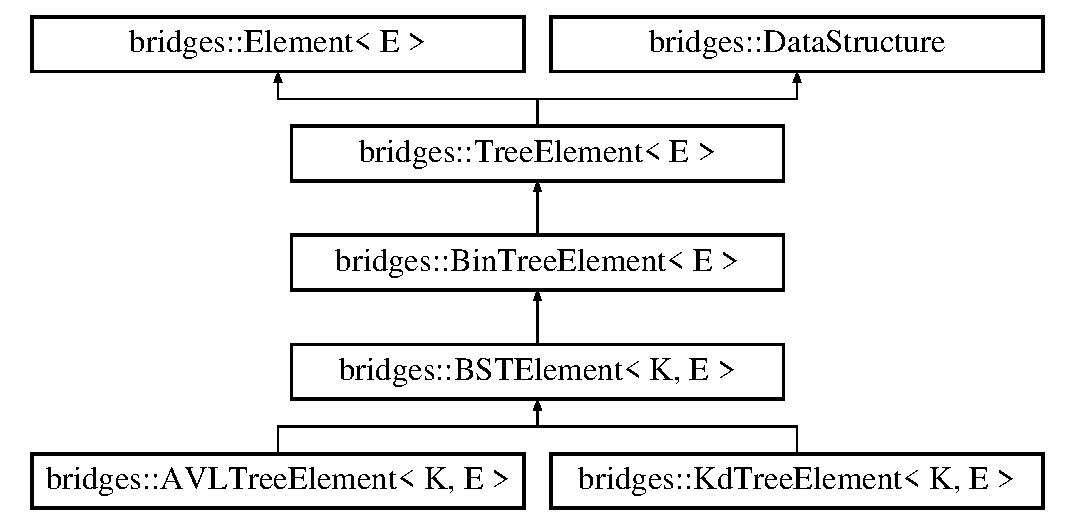
\includegraphics[height=5.000000cm]{classbridges_1_1_tree_element}
\end{center}
\end{figure}
\subsection*{Public Member Functions}
\begin{DoxyCompactItemize}
\item 
\hyperlink{classbridges_1_1_tree_element_a4e96ffab9a6c711ead687dd8a42e80a0}{Tree\+Element} (const E \&e=E(), const string \&lab=string())
\item 
virtual const string \hyperlink{classbridges_1_1_tree_element_a6b264d7391442a742edf96bdd5ee5442}{get\+D\+Stype} () const override
\item 
vector$<$ \hyperlink{classbridges_1_1_tree_element}{Tree\+Element} $\ast$ $>$ \& \hyperlink{classbridges_1_1_tree_element_a52cb83546da21674d306cbb8026f89ac}{get\+Children} ()
\item 
const vector$<$ \hyperlink{classbridges_1_1_tree_element}{Tree\+Element} $\ast$ $>$ \& \hyperlink{classbridges_1_1_tree_element_a5695c33c22a81a3225fa7b37c2bdf34f}{get\+Children} () const
\item 
\hyperlink{classbridges_1_1_tree_element}{Tree\+Element} $\ast$ \hyperlink{classbridges_1_1_tree_element_a14ce2d5b3a4df29c93a0c37dbe73f7a5}{get\+Child} (const int \&n)
\item 
const \hyperlink{classbridges_1_1_tree_element}{Tree\+Element} $\ast$ \hyperlink{classbridges_1_1_tree_element_a23321ef35ce04dd09487824af804e27b}{get\+Child} (const int \&n) const
\item 
void \hyperlink{classbridges_1_1_tree_element_a5e252fa16df0e673526ba4b08c8d3203}{add\+Child} (\hyperlink{classbridges_1_1_tree_element}{Tree\+Element} $\ast$child)
\item 
void \hyperlink{classbridges_1_1_tree_element_aa12cb7cb4b4f559bdf0967872b0a6e7d}{set\+Child} (const size\+\_\+t \&index, \hyperlink{classbridges_1_1_tree_element}{Tree\+Element} $\ast$kid)
\item 
virtual void \hyperlink{classbridges_1_1_tree_element_aad832c9f8dfd7e92c7b06a825f406e1d}{cleanup} () override
\end{DoxyCompactItemize}
\subsection*{Additional Inherited Members}


\subsection{Detailed Description}
\subsubsection*{template$<$typename E$>$\newline
class bridges\+::\+Tree\+Element$<$ E $>$}

This class can be used to create tree elements, derived from \hyperlink{classbridges_1_1_element}{Element}. 

This class can be used to create tree elements, with subtrees

Generic Parameters\+: E the application data type

\begin{DoxyAuthor}{Author}
Kalpathi Subramanian, Dakota Carmer 
\end{DoxyAuthor}
\begin{DoxyDate}{Date}
6/12/15 
\end{DoxyDate}


\subsection{Constructor \& Destructor Documentation}
\hypertarget{classbridges_1_1_tree_element_a4e96ffab9a6c711ead687dd8a42e80a0}{}\label{classbridges_1_1_tree_element_a4e96ffab9a6c711ead687dd8a42e80a0} 
\index{bridges\+::\+Tree\+Element@{bridges\+::\+Tree\+Element}!Tree\+Element@{Tree\+Element}}
\index{Tree\+Element@{Tree\+Element}!bridges\+::\+Tree\+Element@{bridges\+::\+Tree\+Element}}
\subsubsection{\texorpdfstring{Tree\+Element()}{TreeElement()}}
{\footnotesize\ttfamily template$<$typename E$>$ \\
\hyperlink{classbridges_1_1_tree_element}{bridges\+::\+Tree\+Element}$<$ E $>$\+::\hyperlink{classbridges_1_1_tree_element}{Tree\+Element} (\begin{DoxyParamCaption}\item[{const E \&}]{e = {\ttfamily E()},  }\item[{const string \&}]{lab = {\ttfamily string()} }\end{DoxyParamCaption})\hspace{0.3cm}{\ttfamily [inline]}}

Constructs a \hyperlink{classbridges_1_1_tree_element}{Tree\+Element} with the provided value and label, setting the left and right Tree\+Elements to N\+U\+LL. The defaults will be used if not provided.


\begin{DoxyParams}{Parameters}
{\em val} & The data to hold \\
\hline
{\em lab} & The label to show \\
\hline
\end{DoxyParams}


\subsection{Member Function Documentation}
\hypertarget{classbridges_1_1_tree_element_a5e252fa16df0e673526ba4b08c8d3203}{}\label{classbridges_1_1_tree_element_a5e252fa16df0e673526ba4b08c8d3203} 
\index{bridges\+::\+Tree\+Element@{bridges\+::\+Tree\+Element}!add\+Child@{add\+Child}}
\index{add\+Child@{add\+Child}!bridges\+::\+Tree\+Element@{bridges\+::\+Tree\+Element}}
\subsubsection{\texorpdfstring{add\+Child()}{addChild()}}
{\footnotesize\ttfamily template$<$typename E$>$ \\
void \hyperlink{classbridges_1_1_tree_element}{bridges\+::\+Tree\+Element}$<$ E $>$\+::add\+Child (\begin{DoxyParamCaption}\item[{\hyperlink{classbridges_1_1_tree_element}{Tree\+Element}$<$ E $>$ $\ast$}]{child }\end{DoxyParamCaption})\hspace{0.3cm}{\ttfamily [inline]}}

Adds a child to children


\begin{DoxyParams}{Parameters}
{\em kid} & The child \hyperlink{classbridges_1_1_tree_element}{Tree\+Element} \\
\hline
\end{DoxyParams}
\begin{DoxyReturn}{Returns}
index of child 
\end{DoxyReturn}
\hypertarget{classbridges_1_1_tree_element_aad832c9f8dfd7e92c7b06a825f406e1d}{}\label{classbridges_1_1_tree_element_aad832c9f8dfd7e92c7b06a825f406e1d} 
\index{bridges\+::\+Tree\+Element@{bridges\+::\+Tree\+Element}!cleanup@{cleanup}}
\index{cleanup@{cleanup}!bridges\+::\+Tree\+Element@{bridges\+::\+Tree\+Element}}
\subsubsection{\texorpdfstring{cleanup()}{cleanup()}}
{\footnotesize\ttfamily template$<$typename E$>$ \\
virtual void \hyperlink{classbridges_1_1_tree_element}{bridges\+::\+Tree\+Element}$<$ E $>$\+::cleanup (\begin{DoxyParamCaption}{ }\end{DoxyParamCaption})\hspace{0.3cm}{\ttfamily [inline]}, {\ttfamily [override]}, {\ttfamily [virtual]}}

Calls delete on itself and each next linked Tree\+Element$\ast$

\begin{DoxyWarning}{Warning}
Only call if these Tree\+Elements were all dynamicaly allocated( aka\+: using new) 

If tree contains redundant links, delete will be called multiple times on it, leading to undefined behavior 
\end{DoxyWarning}


Reimplemented from \hyperlink{classbridges_1_1_data_structure_ac3ad75810fd77f0ad35b9b5123d2c8f8}{bridges\+::\+Data\+Structure}.

\hypertarget{classbridges_1_1_tree_element_a14ce2d5b3a4df29c93a0c37dbe73f7a5}{}\label{classbridges_1_1_tree_element_a14ce2d5b3a4df29c93a0c37dbe73f7a5} 
\index{bridges\+::\+Tree\+Element@{bridges\+::\+Tree\+Element}!get\+Child@{get\+Child}}
\index{get\+Child@{get\+Child}!bridges\+::\+Tree\+Element@{bridges\+::\+Tree\+Element}}
\subsubsection{\texorpdfstring{get\+Child()}{getChild()}\hspace{0.1cm}{\footnotesize\ttfamily [1/2]}}
{\footnotesize\ttfamily template$<$typename E$>$ \\
\hyperlink{classbridges_1_1_tree_element}{Tree\+Element}$\ast$ \hyperlink{classbridges_1_1_tree_element}{bridges\+::\+Tree\+Element}$<$ E $>$\+::get\+Child (\begin{DoxyParamCaption}\item[{const int \&}]{n }\end{DoxyParamCaption})\hspace{0.3cm}{\ttfamily [inline]}}

Gets the nth child of this \hyperlink{classbridges_1_1_tree_element}{Tree\+Element}, returns null if non-\/existent


\begin{DoxyParams}{Parameters}
{\em n} & The index of the child \\
\hline
\end{DoxyParams}
\begin{DoxyReturn}{Returns}
The child \hyperlink{classbridges_1_1_tree_element}{Tree\+Element} 
\end{DoxyReturn}
\hypertarget{classbridges_1_1_tree_element_a23321ef35ce04dd09487824af804e27b}{}\label{classbridges_1_1_tree_element_a23321ef35ce04dd09487824af804e27b} 
\index{bridges\+::\+Tree\+Element@{bridges\+::\+Tree\+Element}!get\+Child@{get\+Child}}
\index{get\+Child@{get\+Child}!bridges\+::\+Tree\+Element@{bridges\+::\+Tree\+Element}}
\subsubsection{\texorpdfstring{get\+Child()}{getChild()}\hspace{0.1cm}{\footnotesize\ttfamily [2/2]}}
{\footnotesize\ttfamily template$<$typename E$>$ \\
const \hyperlink{classbridges_1_1_tree_element}{Tree\+Element}$\ast$ \hyperlink{classbridges_1_1_tree_element}{bridges\+::\+Tree\+Element}$<$ E $>$\+::get\+Child (\begin{DoxyParamCaption}\item[{const int \&}]{n }\end{DoxyParamCaption}) const\hspace{0.3cm}{\ttfamily [inline]}}

Constant version

Gets the nth child of this \hyperlink{classbridges_1_1_tree_element}{Tree\+Element}, returns null if non-\/existent


\begin{DoxyParams}{Parameters}
{\em n} & The index of the child \\
\hline
\end{DoxyParams}
\begin{DoxyReturn}{Returns}
The child \hyperlink{classbridges_1_1_tree_element}{Tree\+Element} 
\end{DoxyReturn}
\hypertarget{classbridges_1_1_tree_element_a52cb83546da21674d306cbb8026f89ac}{}\label{classbridges_1_1_tree_element_a52cb83546da21674d306cbb8026f89ac} 
\index{bridges\+::\+Tree\+Element@{bridges\+::\+Tree\+Element}!get\+Children@{get\+Children}}
\index{get\+Children@{get\+Children}!bridges\+::\+Tree\+Element@{bridges\+::\+Tree\+Element}}
\subsubsection{\texorpdfstring{get\+Children()}{getChildren()}\hspace{0.1cm}{\footnotesize\ttfamily [1/2]}}
{\footnotesize\ttfamily template$<$typename E$>$ \\
vector$<$\hyperlink{classbridges_1_1_tree_element}{Tree\+Element}$\ast$$>$\& \hyperlink{classbridges_1_1_tree_element}{bridges\+::\+Tree\+Element}$<$ E $>$\+::get\+Children (\begin{DoxyParamCaption}{ }\end{DoxyParamCaption})\hspace{0.3cm}{\ttfamily [inline]}}

\begin{DoxyReturn}{Returns}
The children Tree\+Elements 
\end{DoxyReturn}
\hypertarget{classbridges_1_1_tree_element_a5695c33c22a81a3225fa7b37c2bdf34f}{}\label{classbridges_1_1_tree_element_a5695c33c22a81a3225fa7b37c2bdf34f} 
\index{bridges\+::\+Tree\+Element@{bridges\+::\+Tree\+Element}!get\+Children@{get\+Children}}
\index{get\+Children@{get\+Children}!bridges\+::\+Tree\+Element@{bridges\+::\+Tree\+Element}}
\subsubsection{\texorpdfstring{get\+Children()}{getChildren()}\hspace{0.1cm}{\footnotesize\ttfamily [2/2]}}
{\footnotesize\ttfamily template$<$typename E$>$ \\
const vector$<$\hyperlink{classbridges_1_1_tree_element}{Tree\+Element}$\ast$$>$\& \hyperlink{classbridges_1_1_tree_element}{bridges\+::\+Tree\+Element}$<$ E $>$\+::get\+Children (\begin{DoxyParamCaption}{ }\end{DoxyParamCaption}) const\hspace{0.3cm}{\ttfamily [inline]}}

Constant version

\begin{DoxyReturn}{Returns}
The children Tree\+Elements 
\end{DoxyReturn}
\hypertarget{classbridges_1_1_tree_element_a6b264d7391442a742edf96bdd5ee5442}{}\label{classbridges_1_1_tree_element_a6b264d7391442a742edf96bdd5ee5442} 
\index{bridges\+::\+Tree\+Element@{bridges\+::\+Tree\+Element}!get\+D\+Stype@{get\+D\+Stype}}
\index{get\+D\+Stype@{get\+D\+Stype}!bridges\+::\+Tree\+Element@{bridges\+::\+Tree\+Element}}
\subsubsection{\texorpdfstring{get\+D\+Stype()}{getDStype()}}
{\footnotesize\ttfamily template$<$typename E$>$ \\
virtual const string \hyperlink{classbridges_1_1_tree_element}{bridges\+::\+Tree\+Element}$<$ E $>$\+::get\+D\+Stype (\begin{DoxyParamCaption}{ }\end{DoxyParamCaption}) const\hspace{0.3cm}{\ttfamily [inline]}, {\ttfamily [override]}, {\ttfamily [virtual]}}

\begin{DoxyReturn}{Returns}
The string representation of this data structure type 
\end{DoxyReturn}


Implements \hyperlink{classbridges_1_1_data_structure_a957a63b106e340bc753620c650632bdc}{bridges\+::\+Data\+Structure}.



Reimplemented in \hyperlink{classbridges_1_1_b_t_element_a43cc18d2c1e71c399782a306b60e4260}{bridges\+::\+B\+T\+Element$<$ E $>$}, \hyperlink{classbridges_1_1_b_s_t_element_af3843873c508c24f90b6e73a6f490bf8}{bridges\+::\+B\+S\+T\+Element$<$ K, E $>$}, \hyperlink{classbridges_1_1_bin_tree_element_a0a154f68ef0a58715e598a6ef92b9e59}{bridges\+::\+Bin\+Tree\+Element$<$ E $>$}, and \hyperlink{classbridges_1_1_a_v_l_tree_element_a24c005f8e07a7a2682225cead3b7e364}{bridges\+::\+A\+V\+L\+Tree\+Element$<$ K, E $>$}.

\hypertarget{classbridges_1_1_tree_element_aa12cb7cb4b4f559bdf0967872b0a6e7d}{}\label{classbridges_1_1_tree_element_aa12cb7cb4b4f559bdf0967872b0a6e7d} 
\index{bridges\+::\+Tree\+Element@{bridges\+::\+Tree\+Element}!set\+Child@{set\+Child}}
\index{set\+Child@{set\+Child}!bridges\+::\+Tree\+Element@{bridges\+::\+Tree\+Element}}
\subsubsection{\texorpdfstring{set\+Child()}{setChild()}}
{\footnotesize\ttfamily template$<$typename E$>$ \\
void \hyperlink{classbridges_1_1_tree_element}{bridges\+::\+Tree\+Element}$<$ E $>$\+::set\+Child (\begin{DoxyParamCaption}\item[{const size\+\_\+t \&}]{index,  }\item[{\hyperlink{classbridges_1_1_tree_element}{Tree\+Element}$<$ E $>$ $\ast$}]{kid }\end{DoxyParamCaption})\hspace{0.3cm}{\ttfamily [inline]}}

Sets child at index to \char`\"{}kid\char`\"{}. Will do nothing given invalid index.


\begin{DoxyParams}{Parameters}
{\em index} & of child to replace \\
\hline
{\em kid} & The child \hyperlink{classbridges_1_1_tree_element}{Tree\+Element} \\
\hline
\end{DoxyParams}
This simply replaces the element at position index and the old element is lost(actually can create memory leak if it came from dynamic memory Since we cannot distinguish from allocated or static memory from pointers, it is the user\textquotesingle{}s responsibility to keep track of allocated memory its linkage. For new elements, if not null, create linkage

The documentation for this class was generated from the following file\+:\begin{DoxyCompactItemize}
\item 
/\+Users/kalpathi/gr/bridges/client/cxx/git-\/cxx/src/\hyperlink{_tree_element_8h}{Tree\+Element.\+h}\end{DoxyCompactItemize}

\chapter{File Documentation}
\hypertarget{_array_8h}{}\section{/\+Users/krs/gr/bridges/bridges17/cxx/src/\+Array.h File Reference}
\label{_array_8h}\index{/\+Users/krs/gr/bridges/bridges17/cxx/src/\+Array.\+h@{/\+Users/krs/gr/bridges/bridges17/cxx/src/\+Array.\+h}}
{\ttfamily \#include \char`\"{}Element.\+h\char`\"{}}\\*
{\ttfamily \#include \char`\"{}Bridges.\+h\char`\"{}}\\*
\subsection*{Classes}
\begin{DoxyCompactItemize}
\item 
class \hyperlink{classbridges_1_1_array}{bridges\+::\+Array$<$ E $>$}
\begin{DoxyCompactList}\small\item\em A B\+R\+I\+D\+G\+E\+S array type. \end{DoxyCompactList}\end{DoxyCompactItemize}
\subsection*{Namespaces}
\begin{DoxyCompactItemize}
\item 
 \hyperlink{namespacebridges}{bridges}
\begin{DoxyCompactList}\small\item\em This class can be used to create arrays of type Element$<$\+E$>$ where E is a generic type representation application specific data. Arrays are internally represented as 1\+D arrays; currently 1\+D, 2\+D and 3\+D arrays are supported. \end{DoxyCompactList}\end{DoxyCompactItemize}

\hypertarget{_a_v_l_tree_element_8h}{}\section{/\+Users/kalpathi/gr/bridges/bridges17/cxx/src/\+A\+V\+L\+Tree\+Element.h File Reference}
\label{_a_v_l_tree_element_8h}\index{/\+Users/kalpathi/gr/bridges/bridges17/cxx/src/\+A\+V\+L\+Tree\+Element.\+h@{/\+Users/kalpathi/gr/bridges/bridges17/cxx/src/\+A\+V\+L\+Tree\+Element.\+h}}
{\ttfamily \#include \char`\"{}B\+S\+T\+Element.\+h\char`\"{}}\\*
\subsection*{Classes}
\begin{DoxyCompactItemize}
\item 
class \hyperlink{classbridges_1_1_a_v_l_tree_element}{bridges\+::\+A\+V\+L\+Tree\+Element$<$ K, E $>$}
\begin{DoxyCompactList}\small\item\em This class can be used to create avl tree elements, derived from \hyperlink{classbridges_1_1_b_s_t_element}{B\+S\+T\+Element}. \end{DoxyCompactList}\end{DoxyCompactItemize}
\subsection*{Namespaces}
\begin{DoxyCompactItemize}
\item 
 \hyperlink{namespacebridges}{bridges}
\begin{DoxyCompactList}\small\item\em This class can be used to create arrays of type Element$<$\+E$>$ where E is a generic type representation application specific data. Arrays are internally represented as 1\+D arrays; currently 1\+D, 2\+D and 3\+D arrays are supported. \end{DoxyCompactList}\end{DoxyCompactItemize}

\hypertarget{base64_8h}{}\doxysection{/home/erik/work/bridges/bridges-\/cxx/src/base64.h File Reference}
\label{base64_8h}\index{/home/erik/work/bridges/bridges-\/cxx/src/base64.h@{/home/erik/work/bridges/bridges-\/cxx/src/base64.h}}
{\ttfamily \#include $<$iostream$>$}\newline
{\ttfamily \#include $<$string$>$}\newline
{\ttfamily \#include $<$vector$>$}\newline
\doxysubsection*{Namespaces}
\begin{DoxyCompactItemize}
\item 
 \mbox{\hyperlink{namespacebridges}{bridges}}
\begin{DoxyCompactList}\small\item\em these methods convert byte arrays in to \mbox{\hyperlink{namespacebridges_1_1base64}{base64}} codes and are used in BRIDGES to represent the color arrays as strings. The code is adapted from external sources detailed below. \end{DoxyCompactList}\item 
 \mbox{\hyperlink{namespacebridges_1_1base64}{bridges\+::base64}}
\end{DoxyCompactItemize}
\doxysubsection*{Typedefs}
\begin{DoxyCompactItemize}
\item 
typedef unsigned char \mbox{\hyperlink{namespacebridges_a59b77ee45243ba85c701fb8ab298ef00}{bridges\+::\+BYTE}}
\end{DoxyCompactItemize}
\doxysubsection*{Functions}
\begin{DoxyCompactItemize}
\item 
bool \mbox{\hyperlink{namespacebridges_1_1base64_a2c69d94056dd3848383298e8dde53070}{bridges\+::base64\+::is\+\_\+base64}} (BYTE c)
\item 
string \mbox{\hyperlink{namespacebridges_1_1base64_adf6128e9ca10e7b846b12d8d7346599f}{bridges\+::base64\+::encode}} (BYTE const $\ast$buf, unsigned int buf\+Len)
\item 
vector$<$ BYTE $>$ \mbox{\hyperlink{namespacebridges_1_1base64_ace63480f0930bdabbb26e513f7ef1788}{bridges\+::base64\+::decode}} (string const \&encoded\+\_\+string)
\end{DoxyCompactItemize}
\doxysubsection*{Variables}
\begin{DoxyCompactItemize}
\item 
const string \mbox{\hyperlink{namespacebridges_1_1base64_a6c8692c1898b73649fcb377749e9612a}{bridges\+::base64\+::base64\+\_\+chars}}
\end{DoxyCompactItemize}

\hypertarget{_bin_tree_element_8h}{}\section{/\+Users/krs/gr/bridges/client/cxx/src/\+Bin\+Tree\+Element.h File Reference}
\label{_bin_tree_element_8h}\index{/\+Users/krs/gr/bridges/client/cxx/src/\+Bin\+Tree\+Element.\+h@{/\+Users/krs/gr/bridges/client/cxx/src/\+Bin\+Tree\+Element.\+h}}
{\ttfamily \#include \char`\"{}Tree\+Element.\+h\char`\"{}}\\*
\subsection*{Classes}
\begin{DoxyCompactItemize}
\item 
class \hyperlink{classbridges_1_1_bin_tree_element}{bridges\+::\+Bin\+Tree\+Element$<$ E $>$}
\begin{DoxyCompactList}\small\item\em This class can be used to create binary tree elements, derived from \hyperlink{classbridges_1_1_tree_element}{Tree\+Element}. \end{DoxyCompactList}\end{DoxyCompactItemize}
\subsection*{Namespaces}
\begin{DoxyCompactItemize}
\item 
 \hyperlink{namespacebridges}{bridges}
\begin{DoxyCompactList}\small\item\em This class can be used to create arrays of type Element$<$\+E$>$ where E is a generic type representation application specific data. Arrays are internally represented as 1\+D arrays; currently 1\+D, 2\+D and 3\+D arrays are supported. \end{DoxyCompactList}\end{DoxyCompactItemize}

\hypertarget{_bridges_8h}{}\section{/\+Users/kalpathi/gr/bridges/client/cxx/src/\+Bridges.h File Reference}
\label{_bridges_8h}\index{/\+Users/kalpathi/gr/bridges/client/cxx/src/\+Bridges.\+h@{/\+Users/kalpathi/gr/bridges/client/cxx/src/\+Bridges.\+h}}
{\ttfamily \#include $<$iostream$>$}\newline
{\ttfamily \#include $<$algorithm$>$}\newline
{\ttfamily \#include \char`\"{}Data\+Structure.\+h\char`\"{}}\newline
{\ttfamily \#include \char`\"{}Server\+Comm.\+h\char`\"{}}\newline
{\ttfamily \#include $<$J\+S\+O\+Nutil.\+h$>$}\newline
{\ttfamily \#include $<$alltypes.\+h$>$}\newline
{\ttfamily \#include $<$chrono$>$}\newline
\subsection*{Classes}
\begin{DoxyCompactItemize}
\item 
class \mbox{\hyperlink{classbridges_1_1_bridges}{bridges\+::\+Bridges}}
\begin{DoxyCompactList}\small\item\em This class contains methods to connect and transmit a user\textquotesingle{}s data structure representation to the \mbox{\hyperlink{classbridges_1_1_bridges}{Bridges}} server. \end{DoxyCompactList}\end{DoxyCompactItemize}
\subsection*{Namespaces}
\begin{DoxyCompactItemize}
\item 
 \mbox{\hyperlink{namespacebridges}{bridges}}
\begin{DoxyCompactList}\small\item\em these methods convert byte arrays in to \mbox{\hyperlink{namespacebridges_1_1base64}{base64}} codes and are used in B\+R\+I\+D\+G\+ES to represent the color arrays as strings. The code is adapted from external sources detailed below. \end{DoxyCompactList}\item 
 \mbox{\hyperlink{namespacebridges_1_1game}{bridges\+::game}}
\end{DoxyCompactItemize}

\hypertarget{_bridges2_8h}{}\section{/\+Users/kalpathi/gr/bridges/bridges17/cxx/src/\+Bridges2.h File Reference}
\label{_bridges2_8h}\index{/\+Users/kalpathi/gr/bridges/bridges17/cxx/src/\+Bridges2.\+h@{/\+Users/kalpathi/gr/bridges/bridges17/cxx/src/\+Bridges2.\+h}}
{\ttfamily \#include $<$iostream$>$}\\*
{\ttfamily \#include \char`\"{}Data\+Structure.\+h\char`\"{}}\\*
{\ttfamily \#include \char`\"{}Server\+Comm.\+h\char`\"{}}\\*
\subsection*{Namespaces}
\begin{DoxyCompactItemize}
\item 
 \hyperlink{namespacebridges}{bridges}
\begin{DoxyCompactList}\small\item\em This class can be used to create arrays of type Element$<$\+E$>$ where E is a generic type representation application specific data. Arrays are internally represented as 1\+D arrays; currently 1\+D, 2\+D and 3\+D arrays are supported. \end{DoxyCompactList}\item 
 \hyperlink{namespacebridges_1_1_bridges}{bridges\+::\+Bridges}
\begin{DoxyCompactList}\small\item\em This class contains methods to connect and transmit a user\textquotesingle{}s data structure representation to the \hyperlink{namespacebridges_1_1_bridges}{Bridges} server (up to 5000 elements) \end{DoxyCompactList}\end{DoxyCompactItemize}
\subsection*{Functions}
\begin{DoxyCompactItemize}
\item 
bool \& \hyperlink{namespacebridges_1_1_bridges_a692124feb006d58c277db36c2e9342c8}{bridges\+::\+Bridges\+::visualize\+J\+S\+O\+N} ()
\item 
void \hyperlink{namespacebridges_1_1_bridges_abb0f749a6dbcd0a430504f66de1dbe64}{bridges\+::\+Bridges\+::visualize\+J\+S\+O\+N} (bool flag)
\item 
string \& \hyperlink{namespacebridges_1_1_bridges_a98c0c6658b8eb9e8f20a7f3119cbd984}{bridges\+::\+Bridges\+::user\+Name} ()
\item 
string \& \hyperlink{namespacebridges_1_1_bridges_a4ec319d8c731624bd1aa0efa2427044e}{bridges\+::\+Bridges\+::api\+Key} ()
\item 
unsigned int \& \hyperlink{namespacebridges_1_1_bridges_a97d6cfdc40ecead5d802ac2054933038}{bridges\+::\+Bridges\+::assignment} ()
\item 
string \& \hyperlink{namespacebridges_1_1_bridges_a6a7303bf89edfe41c19f30b4cc6430b9}{bridges\+::\+Bridges\+::get\+Title} ()
\item 
void \hyperlink{namespacebridges_1_1_bridges_af36e132d582dabf5ae5ee8b8f26976db}{bridges\+::\+Bridges\+::set\+Title} (string t)
\item 
string \& \hyperlink{namespacebridges_1_1_bridges_a11570abeb2d710440c709bafca816a64}{bridges\+::\+Bridges\+::get\+Description} ()
\item 
void \hyperlink{namespacebridges_1_1_bridges_ada1bced1a3d7af3b8b139bbdfba72fc8}{bridges\+::\+Bridges\+::set\+Description} (string descr)
\item 
void \hyperlink{namespacebridges_1_1_bridges_a1eef7c2daeb3784169965f727bf4ad1b}{bridges\+::\+Bridges\+::set\+Dimensions} (int $\ast$d)
\item 
void \hyperlink{namespacebridges_1_1_bridges_a7447e2d5808c492d26132690c1a639a7}{bridges\+::\+Bridges\+::set\+Data\+Structure} (Data\+Structure $\ast$ds)
\item 
Data\+Structure $\ast$\& \hyperlink{namespacebridges_1_1_bridges_a7cee9c57a0cd6a213722ba0a81a742f0}{bridges\+::\+Bridges\+::get\+Data\+Structure} ()
\item 
void \hyperlink{namespacebridges_1_1_bridges_a10272250ed6f4bb8281dcaecc61fa698}{bridges\+::\+Bridges\+::initialize} (const unsigned int \&num, const string \&name, const string \&key)
\item 
void \hyperlink{namespacebridges_1_1_bridges_a2806e395134614cdd6327400b53d28ad}{bridges\+::\+Bridges\+::visualize} ()
\end{DoxyCompactItemize}

\hypertarget{_b_s_t_element_8h}{}\section{/\+Users/krs/gr/bridges/client/cxx/src/\+B\+S\+T\+Element.h File Reference}
\label{_b_s_t_element_8h}\index{/\+Users/krs/gr/bridges/client/cxx/src/\+B\+S\+T\+Element.\+h@{/\+Users/krs/gr/bridges/client/cxx/src/\+B\+S\+T\+Element.\+h}}
{\ttfamily \#include $<$sstream$>$}\\*
{\ttfamily \#include \char`\"{}Bin\+Tree\+Element.\+h\char`\"{}}\\*
{\ttfamily \#include $<$J\+S\+O\+Nutil.\+h$>$}\\*
\subsection*{Classes}
\begin{DoxyCompactItemize}
\item 
class \hyperlink{classbridges_1_1_b_s_t_element}{bridges\+::\+B\+S\+T\+Element$<$ K, E $>$}
\begin{DoxyCompactList}\small\item\em This class can be used to create binary search tree elements, derived from \hyperlink{classbridges_1_1_bin_tree_element}{Bin\+Tree\+Element}. \end{DoxyCompactList}\end{DoxyCompactItemize}
\subsection*{Namespaces}
\begin{DoxyCompactItemize}
\item 
 \hyperlink{namespacebridges}{bridges}
\begin{DoxyCompactList}\small\item\em This class can be used to create arrays of type Element$<$\+E$>$ where E is a generic type representation application specific data. Arrays are internally represented as 1\+D arrays; currently 1\+D, 2\+D and 3\+D arrays are supported. \end{DoxyCompactList}\end{DoxyCompactItemize}

\hypertarget{_b_t_element_8h}{}\section{/\+Users/kalpathi/gr/bridges/client/cxx/git-\/cxx/src/\+B\+T\+Element.h File Reference}
\label{_b_t_element_8h}\index{/\+Users/kalpathi/gr/bridges/client/cxx/git-\/cxx/src/\+B\+T\+Element.\+h@{/\+Users/kalpathi/gr/bridges/client/cxx/git-\/cxx/src/\+B\+T\+Element.\+h}}
{\ttfamily \#include \char`\"{}Tree\+Element.\+h\char`\"{}}\newline
\subsection*{Classes}
\begin{DoxyCompactItemize}
\item 
class \hyperlink{classbridges_1_1_b_t_element}{bridges\+::\+B\+T\+Element$<$ E $>$}
\begin{DoxyCompactList}\small\item\em This class can be used to create binary tree elements, derived from \hyperlink{classbridges_1_1_tree_element}{Tree\+Element}. \end{DoxyCompactList}\end{DoxyCompactItemize}
\subsection*{Namespaces}
\begin{DoxyCompactItemize}
\item 
 \hyperlink{namespacebridges}{bridges}
\begin{DoxyCompactList}\small\item\em This class can be used to instantiate Circular Doubly Linked List Elements. \end{DoxyCompactList}\end{DoxyCompactItemize}

\hypertarget{_circ_d_lelement_8h}{}\doxysection{/\+Users/kalpathi/gr/bridges/client/c++/src/\+Circ\+D\+Lelement.h File Reference}
\label{_circ_d_lelement_8h}\index{/Users/kalpathi/gr/bridges/client/c++/src/CircDLelement.h@{/Users/kalpathi/gr/bridges/client/c++/src/CircDLelement.h}}
{\ttfamily \#include \char`\"{}D\+Lelement.\+h\char`\"{}}\newline
\doxysubsection*{Classes}
\begin{DoxyCompactItemize}
\item 
class \mbox{\hyperlink{classbridges_1_1_circ_d_lelement}{bridges\+::\+Circ\+D\+Lelement$<$ E $>$}}
\begin{DoxyCompactList}\small\item\em This class can be used to instantiate Circular Doubly Linked List Elements. \end{DoxyCompactList}\end{DoxyCompactItemize}
\doxysubsection*{Namespaces}
\begin{DoxyCompactItemize}
\item 
 \mbox{\hyperlink{namespacebridges}{bridges}}
\begin{DoxyCompactList}\small\item\em This class can be used to create arrays of type Element$<$\+E$>$ where E is a generic type representation application specific data. Arrays are internally represented as 1D arrays; currently 1D, 2D and 3D arrays are supported. \end{DoxyCompactList}\end{DoxyCompactItemize}

\hypertarget{_circ_s_lelement_8h}{}\section{/\+Users/kalpathi/gr/bridges/cxx/src/\+Circ\+S\+Lelement.h File Reference}
\label{_circ_s_lelement_8h}\index{/Users/kalpathi/gr/bridges/cxx/src/CircSLelement.h@{/Users/kalpathi/gr/bridges/cxx/src/CircSLelement.h}}
{\ttfamily \#include \char`\"{}S\+Lelement.\+h\char`\"{}}\newline
\subsection*{Classes}
\begin{DoxyCompactItemize}
\item 
class \mbox{\hyperlink{classbridges_1_1datastructure_1_1_circ_s_lelement}{bridges\+::datastructure\+::\+Circ\+S\+Lelement$<$ E $>$}}
\begin{DoxyCompactList}\small\item\em This class can be used to instantiate Singly Linked Circular List Elements. \end{DoxyCompactList}\end{DoxyCompactItemize}
\subsection*{Namespaces}
\begin{DoxyCompactItemize}
\item 
 \mbox{\hyperlink{namespacebridges}{bridges}}
\begin{DoxyCompactList}\small\item\em these methods convert byte arrays in to \mbox{\hyperlink{namespacebridges_1_1base64}{base64}} codes and are used in B\+R\+I\+D\+G\+ES to represent the color arrays as strings. The code is adapted from external sources detailed below. \end{DoxyCompactList}\item 
 \mbox{\hyperlink{namespacebridges_1_1datastructure}{bridges\+::datastructure}}
\end{DoxyCompactItemize}

\hypertarget{_color_8h}{}\section{/\+Users/kalpathi/gr/bridges/client/cxx/bridges18/src/\+Color.h File Reference}
\label{_color_8h}\index{/\+Users/kalpathi/gr/bridges/client/cxx/bridges18/src/\+Color.\+h@{/\+Users/kalpathi/gr/bridges/client/cxx/bridges18/src/\+Color.\+h}}
{\ttfamily \#include $<$iostream$>$}\newline
{\ttfamily \#include $<$array$>$}\newline
{\ttfamily \#include $<$regex$>$}\newline
{\ttfamily \#include $<$unordered\+\_\+map$>$}\newline
{\ttfamily \#include $<$cmath$>$}\newline
{\ttfamily \#include $<$sstream$>$}\newline
{\ttfamily \#include $<$iomanip$>$}\newline
{\ttfamily \#include \char`\"{}Data\+Structure.\+h\char`\"{}}\newline
\subsection*{Classes}
\begin{DoxyCompactItemize}
\item 
class \mbox{\hyperlink{classbridges_1_1_color}{bridges\+::\+Color}}
\begin{DoxyCompactList}\small\item\em This class represents \mbox{\hyperlink{classbridges_1_1_color}{Color}}, and supports rgba, hexadecimal and named color values. \end{DoxyCompactList}\end{DoxyCompactItemize}
\subsection*{Namespaces}
\begin{DoxyCompactItemize}
\item 
 \mbox{\hyperlink{namespacebridges}{bridges}}
\begin{DoxyCompactList}\small\item\em This class can be used to create arrays of type Element$<$\+E$>$ where E is a generic type representation application specific data. Arrays are internally represented as 1D arrays; currently 1D, 2D and 3D arrays are supported. \end{DoxyCompactList}\end{DoxyCompactItemize}

\hypertarget{_color_grid_8h}{}\section{/\+Users/kalpathi/gr/bridges/cxx/src/\+Color\+Grid.h File Reference}
\label{_color_grid_8h}\index{/Users/kalpathi/gr/bridges/cxx/src/ColorGrid.h@{/Users/kalpathi/gr/bridges/cxx/src/ColorGrid.h}}
{\ttfamily \#include $<$string$>$}\newline
{\ttfamily \#include \char`\"{}Grid.\+h\char`\"{}}\newline
{\ttfamily \#include \char`\"{}Color.\+h\char`\"{}}\newline
{\ttfamily \#include \char`\"{}base64.\+h\char`\"{}}\newline
\subsection*{Classes}
\begin{DoxyCompactItemize}
\item 
class \mbox{\hyperlink{classbridges_1_1datastructure_1_1_color_grid}{bridges\+::datastructure\+::\+Color\+Grid}}
\begin{DoxyCompactList}\small\item\em This is a class in B\+R\+I\+D\+G\+ES for representing an image. \end{DoxyCompactList}\end{DoxyCompactItemize}
\subsection*{Namespaces}
\begin{DoxyCompactItemize}
\item 
 \mbox{\hyperlink{namespacebridges}{bridges}}
\begin{DoxyCompactList}\small\item\em these methods convert byte arrays in to \mbox{\hyperlink{namespacebridges_1_1base64}{base64}} codes and are used in B\+R\+I\+D\+G\+ES to represent the color arrays as strings. The code is adapted from external sources detailed below. \end{DoxyCompactList}\item 
 \mbox{\hyperlink{namespacebridges_1_1datastructure}{bridges\+::datastructure}}
\end{DoxyCompactItemize}

\hypertarget{_actor_movie_i_m_d_b_8h}{}\doxysection{/\+Users/kalpathi/gr/bridges/client/c++/src/data\+\_\+src/\+Actor\+Movie\+I\+M\+DB.h File Reference}
\label{_actor_movie_i_m_d_b_8h}\index{/Users/kalpathi/gr/bridges/client/c++/src/data\_src/ActorMovieIMDB.h@{/Users/kalpathi/gr/bridges/client/c++/src/data\_src/ActorMovieIMDB.h}}
{\ttfamily \#include $<$string$>$}\newline
\doxysubsection*{Classes}
\begin{DoxyCompactItemize}
\item 
class \mbox{\hyperlink{classbridges_1_1_actor_movie_i_m_d_b}{bridges\+::\+Actor\+Movie\+I\+M\+DB}}
\begin{DoxyCompactList}\small\item\em A class to hold actor movie data -- using I\+M\+DB dataset. \end{DoxyCompactList}\end{DoxyCompactItemize}
\doxysubsection*{Namespaces}
\begin{DoxyCompactItemize}
\item 
 \mbox{\hyperlink{namespacebridges}{bridges}}
\begin{DoxyCompactList}\small\item\em This class can be used to create arrays of type Element$<$\+E$>$ where E is a generic type representation application specific data. Arrays are internally represented as 1D arrays; currently 1D, 2D and 3D arrays are supported. \end{DoxyCompactList}\end{DoxyCompactItemize}

\hypertarget{_book_8h}{}\section{/\+Users/kalpathi/gr/bridges/bridges17/cxx/src/data\+\_\+src/\+Book.h File Reference}
\label{_book_8h}\index{/\+Users/kalpathi/gr/bridges/bridges17/cxx/src/data\+\_\+src/\+Book.\+h@{/\+Users/kalpathi/gr/bridges/bridges17/cxx/src/data\+\_\+src/\+Book.\+h}}
{\ttfamily \#include $<$string$>$}\\*
\subsection*{Classes}
\begin{DoxyCompactItemize}
\item 
class \hyperlink{classbridges_1_1_book}{bridges\+::\+Book}
\begin{DoxyCompactList}\small\item\em A \hyperlink{classbridges_1_1_book}{Book} object, used along with the books data source. \end{DoxyCompactList}\end{DoxyCompactItemize}
\subsection*{Namespaces}
\begin{DoxyCompactItemize}
\item 
 \hyperlink{namespacebridges}{bridges}
\begin{DoxyCompactList}\small\item\em This class can be used to create arrays of type Element$<$\+E$>$ where E is a generic type representation application specific data. Arrays are internally represented as 1\+D arrays; currently 1\+D, 2\+D and 3\+D arrays are supported. \end{DoxyCompactList}\end{DoxyCompactItemize}

\hypertarget{_cancer_incidence_8h}{}\section{/\+Users/kalpathi/gr/bridges/cxx/src/data\+\_\+src/\+Cancer\+Incidence.h File Reference}
\label{_cancer_incidence_8h}\index{/Users/kalpathi/gr/bridges/cxx/src/data\_src/CancerIncidence.h@{/Users/kalpathi/gr/bridges/cxx/src/data\_src/CancerIncidence.h}}
{\ttfamily \#include $<$string$>$}\newline
\subsection*{Classes}
\begin{DoxyCompactItemize}
\item 
class \mbox{\hyperlink{classbridges_1_1_cancer_incidence}{bridges\+::\+Cancer\+Incidence}}
\begin{DoxyCompactList}\small\item\em A class representing the attributes for cancer incidence. \end{DoxyCompactList}\end{DoxyCompactItemize}
\subsection*{Namespaces}
\begin{DoxyCompactItemize}
\item 
 \mbox{\hyperlink{namespacebridges}{bridges}}
\begin{DoxyCompactList}\small\item\em This class can be used to create arrays of type Element$<$\+E$>$ where E is a generic type representation application specific data. Arrays are internally represented as 1D arrays; currently 1D, 2D and 3D arrays are supported. \end{DoxyCompactList}\end{DoxyCompactItemize}

\hypertarget{_earthquake_u_s_g_s_8h}{}\section{/\+Users/kalpathi/gr/bridges/client/cxx/bridges17/src/data\+\_\+src/\+Earthquake\+U\+S\+GS.h File Reference}
\label{_earthquake_u_s_g_s_8h}\index{/\+Users/kalpathi/gr/bridges/client/cxx/bridges17/src/data\+\_\+src/\+Earthquake\+U\+S\+G\+S.\+h@{/\+Users/kalpathi/gr/bridges/client/cxx/bridges17/src/data\+\_\+src/\+Earthquake\+U\+S\+G\+S.\+h}}
{\ttfamily \#include $<$string$>$}\newline
\subsection*{Classes}
\begin{DoxyCompactItemize}
\item 
class \mbox{\hyperlink{classbridges_1_1_earthquake_u_s_g_s}{bridges\+::\+Earthquake\+U\+S\+GS}}
\begin{DoxyCompactList}\small\item\em Class that hold earthquake data, for use with U\+S\+G\+IS retrieved quake data. \end{DoxyCompactList}\end{DoxyCompactItemize}
\subsection*{Namespaces}
\begin{DoxyCompactItemize}
\item 
 \mbox{\hyperlink{namespacebridges}{bridges}}
\begin{DoxyCompactList}\small\item\em This class can be used to create arrays of type Element$<$\+E$>$ where E is a generic type representation application specific data. Arrays are internally represented as 1D arrays; currently 1D, 2D and 3D arrays are supported. \end{DoxyCompactList}\end{DoxyCompactItemize}

\hypertarget{_game_8h}{}\section{/\+Users/kalpathi/gr/bridges/cxx/src/data\+\_\+src/\+Game.h File Reference}
\label{_game_8h}\index{/Users/kalpathi/gr/bridges/cxx/src/data\_src/Game.h@{/Users/kalpathi/gr/bridges/cxx/src/data\_src/Game.h}}
{\ttfamily \#include $<$string$>$}\newline
\subsection*{Classes}
\begin{DoxyCompactItemize}
\item 
class \mbox{\hyperlink{classbridges_1_1dataset_1_1_game}{bridges\+::dataset\+::\+Game}}
\begin{DoxyCompactList}\small\item\em A \mbox{\hyperlink{classbridges_1_1dataset_1_1_game}{Game}} object, used along with the Games data source. \end{DoxyCompactList}\end{DoxyCompactItemize}
\subsection*{Namespaces}
\begin{DoxyCompactItemize}
\item 
 \mbox{\hyperlink{namespacebridges}{bridges}}
\begin{DoxyCompactList}\small\item\em these methods convert byte arrays in to \mbox{\hyperlink{namespacebridges_1_1base64}{base64}} codes and are used in B\+R\+I\+D\+G\+ES to represent the color arrays as strings. The code is adapted from external sources detailed below. \end{DoxyCompactList}\item 
 \mbox{\hyperlink{namespacebridges_1_1dataset}{bridges\+::dataset}}
\end{DoxyCompactItemize}

\hypertarget{_gutenberg_book_8h}{}\section{/\+Users/kalpathi/gr/bridges/cxx/src/data\+\_\+src/\+Gutenberg\+Book.h File Reference}
\label{_gutenberg_book_8h}\index{/Users/kalpathi/gr/bridges/cxx/src/data\_src/GutenbergBook.h@{/Users/kalpathi/gr/bridges/cxx/src/data\_src/GutenbergBook.h}}
{\ttfamily \#include $<$string$>$}\newline
\subsection*{Classes}
\begin{DoxyCompactItemize}
\item 
class \mbox{\hyperlink{classbridges_1_1dataset_1_1_gutenberg_book}{bridges\+::dataset\+::\+Gutenberg\+Book}}
\begin{DoxyCompactList}\small\item\em A Gutenberg \mbox{\hyperlink{classbridges_1_1dataset_1_1_book}{Book}} object metadata only, used along with the books data source. \end{DoxyCompactList}\end{DoxyCompactItemize}
\subsection*{Namespaces}
\begin{DoxyCompactItemize}
\item 
 \mbox{\hyperlink{namespacebridges}{bridges}}
\begin{DoxyCompactList}\small\item\em these methods convert byte arrays in to \mbox{\hyperlink{namespacebridges_1_1base64}{base64}} codes and are used in B\+R\+I\+D\+G\+ES to represent the color arrays as strings. The code is adapted from external sources detailed below. \end{DoxyCompactList}\item 
 \mbox{\hyperlink{namespacebridges_1_1dataset}{bridges\+::dataset}}
\end{DoxyCompactItemize}

\hypertarget{_shakespeare_8h}{}\section{/\+Users/krs/gr/bridges/client/cxx/src/data\+\_\+src/\+Shakespeare.h File Reference}
\label{_shakespeare_8h}\index{/\+Users/krs/gr/bridges/client/cxx/src/data\+\_\+src/\+Shakespeare.\+h@{/\+Users/krs/gr/bridges/client/cxx/src/data\+\_\+src/\+Shakespeare.\+h}}
{\ttfamily \#include $<$string$>$}\\*
\subsection*{Classes}
\begin{DoxyCompactItemize}
\item 
class \hyperlink{classbridges_1_1_shakespeare}{bridges\+::\+Shakespeare}
\begin{DoxyCompactList}\small\item\em A \hyperlink{classbridges_1_1_shakespeare}{Shakespeare} book object, used along with the \hyperlink{classbridges_1_1_shakespeare}{Shakespeare} books data source. \end{DoxyCompactList}\end{DoxyCompactItemize}
\subsection*{Namespaces}
\begin{DoxyCompactItemize}
\item 
 \hyperlink{namespacebridges}{bridges}
\begin{DoxyCompactList}\small\item\em This class can be used to create arrays of type Element$<$\+E$>$ where E is a generic type representation application specific data. Arrays are internally represented as 1\+D arrays; currently 1\+D, 2\+D and 3\+D arrays are supported. \end{DoxyCompactList}\end{DoxyCompactItemize}

\hypertarget{_song_8h}{}\section{/\+Users/kalpathi/gr/bridges/cxx/src/data\+\_\+src/\+Song.h File Reference}
\label{_song_8h}\index{/Users/kalpathi/gr/bridges/cxx/src/data\_src/Song.h@{/Users/kalpathi/gr/bridges/cxx/src/data\_src/Song.h}}
\subsection*{Classes}
\begin{DoxyCompactItemize}
\item 
class \mbox{\hyperlink{classbridges_1_1dataset_1_1_song}{bridges\+::dataset\+::\+Song}}
\begin{DoxyCompactList}\small\item\em A \mbox{\hyperlink{classbridges_1_1dataset_1_1_song}{Song}} object, used along with the Songs data source. \end{DoxyCompactList}\end{DoxyCompactItemize}
\subsection*{Namespaces}
\begin{DoxyCompactItemize}
\item 
 \mbox{\hyperlink{namespacebridges}{bridges}}
\begin{DoxyCompactList}\small\item\em these methods convert byte arrays in to \mbox{\hyperlink{namespacebridges_1_1base64}{base64}} codes and are used in B\+R\+I\+D\+G\+ES to represent the color arrays as strings. The code is adapted from external sources detailed below. \end{DoxyCompactList}\item 
 \mbox{\hyperlink{namespacebridges_1_1dataset}{bridges\+::dataset}}
\end{DoxyCompactItemize}

\hypertarget{_data_source_8h}{}\section{/\+Users/kalpathi/gr/bridges/client/cxx/git-\/cxx/src/\+Data\+Source.h File Reference}
\label{_data_source_8h}\index{/\+Users/kalpathi/gr/bridges/client/cxx/git-\/cxx/src/\+Data\+Source.\+h@{/\+Users/kalpathi/gr/bridges/client/cxx/git-\/cxx/src/\+Data\+Source.\+h}}
{\ttfamily \#include $<$vector$>$}\newline
{\ttfamily \#include $<$string$>$}\newline
{\ttfamily \#include $<$rapidjson/document.\+h$>$}\newline
{\ttfamily \#include \char`\"{}Server\+Comm.\+h\char`\"{}}\newline
{\ttfamily \#include \char`\"{}./data\+\_\+src/\+Earthquake\+U\+S\+G\+S.\+h\char`\"{}}\newline
{\ttfamily \#include \char`\"{}./data\+\_\+src/\+Game.\+h\char`\"{}}\newline
{\ttfamily \#include \char`\"{}./data\+\_\+src/\+Shakespeare.\+h\char`\"{}}\newline
{\ttfamily \#include \char`\"{}./data\+\_\+src/\+Book.\+h\char`\"{}}\newline
\subsection*{Namespaces}
\begin{DoxyCompactItemize}
\item 
 \hyperlink{namespacebridges}{bridges}
\begin{DoxyCompactList}\small\item\em This class can be used to instantiate Circular Doubly Linked List Elements. \end{DoxyCompactList}\item 
 \hyperlink{namespacebridges_1_1_data_source}{bridges\+::\+Data\+Source}
\begin{DoxyCompactList}\small\item\em This provides an A\+PI to various data sources used in B\+R\+I\+D\+G\+ES. \end{DoxyCompactList}\end{DoxyCompactItemize}
\subsection*{Functions}
\begin{DoxyCompactItemize}
\item 
vector$<$ Game $>$ \hyperlink{namespacebridges_1_1_data_source_a96a28cc7f2a6013fe09b07cc53c7432f}{bridges\+::\+Data\+Source\+::get\+Game\+Data} ()
\item 
vector$<$ Earthquake\+U\+S\+GS $>$ \hyperlink{namespacebridges_1_1_data_source_a2af96553650d859b102f179b3db55389}{bridges\+::\+Data\+Source\+::get\+Earthquake\+Data} (int number=0)
\item 
vector$<$ Shakespeare $>$ \hyperlink{namespacebridges_1_1_data_source_abdf2e4d709e9b7f1a5370726676d86ec}{bridges\+::\+Data\+Source\+::get\+Shakespeare\+Data} (string endpoint=\char`\"{}\char`\"{}, bool simple=false)
\item 
vector$<$ Book $>$ \hyperlink{namespacebridges_1_1_data_source_aa7f1de628f3ad3309dbf89bd61108990}{bridges\+::\+Data\+Source\+::get\+Book\+Data} (int num=0)
\end{DoxyCompactItemize}

\hypertarget{_data_structure_8h}{}\doxysection{/home/erik/work/bridges/bridges-\/cxx/src/\+Data\+Structure.h File Reference}
\label{_data_structure_8h}\index{/home/erik/work/bridges/bridges-\/cxx/src/DataStructure.h@{/home/erik/work/bridges/bridges-\/cxx/src/DataStructure.h}}
{\ttfamily \#include $<$string$>$}\newline
\doxysubsection*{Classes}
\begin{DoxyCompactItemize}
\item 
class \mbox{\hyperlink{classbridges_1_1datastructure_1_1_data_structure}{bridges\+::datastructure\+::\+Data\+Structure}}
\begin{DoxyCompactList}\small\item\em This is the superclass of all data structure types in BRIDGES. \end{DoxyCompactList}\end{DoxyCompactItemize}
\doxysubsection*{Namespaces}
\begin{DoxyCompactItemize}
\item 
 \mbox{\hyperlink{namespacebridges}{bridges}}
\begin{DoxyCompactList}\small\item\em these methods convert byte arrays in to \mbox{\hyperlink{namespacebridges_1_1base64}{base64}} codes and are used in BRIDGES to represent the color arrays as strings. The code is adapted from external sources detailed below. \end{DoxyCompactList}\item 
 \mbox{\hyperlink{namespacebridges_1_1datastructure}{bridges\+::datastructure}}
\end{DoxyCompactItemize}
\doxysubsection*{Variables}
\begin{DoxyCompactItemize}
\item 
const string \mbox{\hyperlink{namespacebridges_acd8357e88562cbb7e60bea3fac422ac3}{bridges\+::\+QUOTE}} = \char`\"{}\textbackslash{}\char`\"{}\char`\"{}
\item 
const string \mbox{\hyperlink{namespacebridges_a74087afbaa635d3c3d837cc3b44c0162}{bridges\+::\+COMMA}} = \char`\"{},\char`\"{}
\item 
const string \mbox{\hyperlink{namespacebridges_a039dca813ca3a9b4c8d8a866c6fa8445}{bridges\+::\+COLON}} = \char`\"{}\+:\char`\"{}
\item 
const string \mbox{\hyperlink{namespacebridges_a9bef552535e3f5bbfc2ca586cb5044c6}{bridges\+::\+OPEN\+\_\+\+CURLY}} = \char`\"{}\{\char`\"{}
\item 
const string \mbox{\hyperlink{namespacebridges_aa0d8f65415cfe7cdca23401137d40ca9}{bridges\+::\+CLOSE\+\_\+\+CURLY}} = \char`\"{}\}\char`\"{}
\item 
const string \mbox{\hyperlink{namespacebridges_a6b481335016325fe202a4e2fedd0af14}{bridges\+::\+OPEN\+\_\+\+BOX}} = \char`\"{}\mbox{[}\char`\"{}
\item 
const string \mbox{\hyperlink{namespacebridges_a9cbd20a3f223f32670280b954061f274}{bridges\+::\+CLOSE\+\_\+\+BOX}} = \char`\"{}\mbox{]}\char`\"{}
\item 
const string \mbox{\hyperlink{namespacebridges_ad909fb43b05ef6b7271fddbe85e2742a}{bridges\+::\+OPEN\+\_\+\+PARENS}} = \char`\"{}(\char`\"{}
\item 
const string \mbox{\hyperlink{namespacebridges_aff509a0d23b28c17004b1efd5a0a5920}{bridges\+::\+CLOSE\+\_\+\+PARENS}} = \char`\"{})\char`\"{}
\item 
constexpr int \mbox{\hyperlink{namespacebridges_1_1datastructure_a2e75baaa66b6c9cd3f5c5f598b2c8147}{bridges\+::datastructure\+::\+MAX\+\_\+\+ELEMENTS\+\_\+\+ALLOWED}} = 5000
\end{DoxyCompactItemize}

\hypertarget{_d_lelement_8h}{}\doxysection{/\+Users/kalpathi/gr/bridges/client/c++/src/\+D\+Lelement.h File Reference}
\label{_d_lelement_8h}\index{/Users/kalpathi/gr/bridges/client/c++/src/DLelement.h@{/Users/kalpathi/gr/bridges/client/c++/src/DLelement.h}}
{\ttfamily \#include \char`\"{}S\+Lelement.\+h\char`\"{}}\newline
\doxysubsection*{Classes}
\begin{DoxyCompactItemize}
\item 
class \mbox{\hyperlink{classbridges_1_1_d_lelement}{bridges\+::\+D\+Lelement$<$ E $>$}}
\begin{DoxyCompactList}\small\item\em The doubly linked list element, derived from \mbox{\hyperlink{classbridges_1_1_s_lelement}{S\+Lelement}}. \end{DoxyCompactList}\end{DoxyCompactItemize}
\doxysubsection*{Namespaces}
\begin{DoxyCompactItemize}
\item 
 \mbox{\hyperlink{namespacebridges}{bridges}}
\begin{DoxyCompactList}\small\item\em This class can be used to create arrays of type Element$<$\+E$>$ where E is a generic type representation application specific data. Arrays are internally represented as 1D arrays; currently 1D, 2D and 3D arrays are supported. \end{DoxyCompactList}\end{DoxyCompactItemize}

\hypertarget{_edge_8h}{}\section{/\+Users/kalpathi/gr/bridges/cxx/src/\+Edge.h File Reference}
\label{_edge_8h}\index{/Users/kalpathi/gr/bridges/cxx/src/Edge.h@{/Users/kalpathi/gr/bridges/cxx/src/Edge.h}}
{\ttfamily \#include $<$string$>$}\newline
{\ttfamily \#include \char`\"{}Link\+Visualizer.\+h\char`\"{}}\newline
\subsection*{Classes}
\begin{DoxyCompactItemize}
\item 
class \mbox{\hyperlink{classbridges_1_1_edge}{bridges\+::\+Edge$<$ K, E2 $>$}}
\begin{DoxyCompactList}\small\item\em This helper class is used by the graph classes -\/ \mbox{\hyperlink{classbridges_1_1_graph_adj_list}{Graph\+Adj\+List}} , \mbox{\hyperlink{classbridges_1_1_graph_adj_matrix}{Graph\+Adj\+Matrix}} -\/ to keep track of edge information. \end{DoxyCompactList}\end{DoxyCompactItemize}
\subsection*{Namespaces}
\begin{DoxyCompactItemize}
\item 
 \mbox{\hyperlink{namespacebridges}{bridges}}
\begin{DoxyCompactList}\small\item\em This class can be used to create arrays of type Element$<$\+E$>$ where E is a generic type representation application specific data. Arrays are internally represented as 1D arrays; currently 1D, 2D and 3D arrays are supported. \end{DoxyCompactList}\end{DoxyCompactItemize}

\hypertarget{_element_8h}{}\section{/\+Users/kalpathi/gr/bridges/client/cxx/src/\+Element.h File Reference}
\label{_element_8h}\index{/\+Users/kalpathi/gr/bridges/client/cxx/src/\+Element.\+h@{/\+Users/kalpathi/gr/bridges/client/cxx/src/\+Element.\+h}}
{\ttfamily \#include $<$unordered\+\_\+set$>$}\newline
{\ttfamily \#include $<$unordered\+\_\+map$>$}\newline
{\ttfamily \#include $<$cmath$>$}\newline
{\ttfamily \#include \char`\"{}Data\+Structure.\+h\char`\"{}}\newline
{\ttfamily \#include \char`\"{}Element\+Visualizer.\+h\char`\"{}}\newline
{\ttfamily \#include \char`\"{}Link\+Visualizer.\+h\char`\"{}}\newline
{\ttfamily \#include $<$J\+S\+O\+Nutil.\+h$>$}\newline
\subsection*{Classes}
\begin{DoxyCompactItemize}
\item 
class \mbox{\hyperlink{classbridges_1_1datastructure_1_1_graph_adj_list}{bridges\+::datastructure\+::\+Graph\+Adj\+List$<$ K, E1, E2 $>$}}
\begin{DoxyCompactList}\small\item\em This class provides methods to represent adjacency list based graphs. \end{DoxyCompactList}\item 
class \mbox{\hyperlink{classbridges_1_1datastructure_1_1_graph_adj_matrix}{bridges\+::datastructure\+::\+Graph\+Adj\+Matrix$<$ K, E1, E2 $>$}}
\begin{DoxyCompactList}\small\item\em This class provides methods to represent adjacency matrix based graphs. \end{DoxyCompactList}\item 
class \mbox{\hyperlink{classbridges_1_1datastructure_1_1_element}{bridges\+::datastructure\+::\+Element$<$ E $>$}}
\begin{DoxyCompactList}\small\item\em This is the fundamental building block for all data structures in B\+R\+I\+D\+G\+ES. \end{DoxyCompactList}\end{DoxyCompactItemize}
\subsection*{Namespaces}
\begin{DoxyCompactItemize}
\item 
 \mbox{\hyperlink{namespacebridges}{bridges}}
\begin{DoxyCompactList}\small\item\em these methods convert byte arrays in to \mbox{\hyperlink{namespacebridges_1_1base64}{base64}} codes and are used in B\+R\+I\+D\+G\+ES to represent the color arrays as strings. The code is adapted from external sources detailed below. \end{DoxyCompactList}\item 
 \mbox{\hyperlink{namespacebridges_1_1datastructure}{bridges\+::datastructure}}
\end{DoxyCompactItemize}

\hypertarget{_element_array_8h}{}\doxysection{/home/erik/work/bridges/bridges-\/cxx/src/\+Element\+Array.h File Reference}
\label{_element_array_8h}\index{/home/erik/work/bridges/bridges-\/cxx/src/ElementArray.h@{/home/erik/work/bridges/bridges-\/cxx/src/ElementArray.h}}
{\ttfamily \#include \char`\"{}Element.\+h\char`\"{}}\newline
\doxysubsection*{Classes}
\begin{DoxyCompactItemize}
\item 
class \mbox{\hyperlink{classbridges_1_1datastructure_1_1_element_array}{bridges\+::datastructure\+::\+Element\+Array$<$ E, X, Y, Z $>$}}
\begin{DoxyCompactList}\small\item\em Currently unused class, ignore. \end{DoxyCompactList}\end{DoxyCompactItemize}
\doxysubsection*{Namespaces}
\begin{DoxyCompactItemize}
\item 
 \mbox{\hyperlink{namespacebridges}{bridges}}
\begin{DoxyCompactList}\small\item\em these methods convert byte arrays in to \mbox{\hyperlink{namespacebridges_1_1base64}{base64}} codes and are used in BRIDGES to represent the color arrays as strings. The code is adapted from external sources detailed below. \end{DoxyCompactList}\item 
 \mbox{\hyperlink{namespacebridges_1_1datastructure}{bridges\+::datastructure}}
\end{DoxyCompactItemize}

\hypertarget{_element_visualizer_8h}{}\section{/\+Users/krs/gr/bridges/cxx/git-\/cxx/src/\+Element\+Visualizer.h File Reference}
\label{_element_visualizer_8h}\index{/\+Users/krs/gr/bridges/cxx/git-\/cxx/src/\+Element\+Visualizer.\+h@{/\+Users/krs/gr/bridges/cxx/git-\/cxx/src/\+Element\+Visualizer.\+h}}
{\ttfamily \#include \char`\"{}Color.\+h\char`\"{}}\\*
\subsection*{Classes}
\begin{DoxyCompactItemize}
\item 
class \hyperlink{classbridges_1_1_element_visualizer}{bridges\+::\+Element\+Visualizer}
\begin{DoxyCompactList}\small\item\em This class maintains the visual properties of the a \hyperlink{namespacebridges_1_1_bridges}{Bridges} element. \end{DoxyCompactList}\end{DoxyCompactItemize}
\subsection*{Namespaces}
\begin{DoxyCompactItemize}
\item 
 \hyperlink{namespacebridges}{bridges}
\begin{DoxyCompactList}\small\item\em This helper class is used by the graph classes -\/ \hyperlink{classbridges_1_1_graph_adj_list}{Graph\+Adj\+List} , \hyperlink{classbridges_1_1_graph_adj_matrix}{Graph\+Adj\+Matrix} -\/ to keep track of edge information. \end{DoxyCompactList}\end{DoxyCompactItemize}
\subsection*{Enumerations}
\begin{DoxyCompactItemize}
\item 
enum \hyperlink{namespacebridges_a1b4050586bd708782ae0d4f3b06b9579}{bridges\+::\+Shape} \{ \\*
\hyperlink{namespacebridges_a1b4050586bd708782ae0d4f3b06b9579aa968bf0f7aeccbae1a40751345bf2e64}{bridges\+::\+C\+I\+R\+C\+L\+E}, 
\hyperlink{namespacebridges_a1b4050586bd708782ae0d4f3b06b9579a4fc84095f1e7f3e664913b93050196e2}{bridges\+::\+S\+Q\+U\+A\+R\+E}, 
\hyperlink{namespacebridges_a1b4050586bd708782ae0d4f3b06b9579aefd26c044477c7b165bc744110e0ee93}{bridges\+::\+D\+I\+A\+M\+O\+N\+D}, 
\hyperlink{namespacebridges_a1b4050586bd708782ae0d4f3b06b9579abe7bf91f3fc0356925109d7afdd43135}{bridges\+::\+C\+R\+O\+S\+S}, 
\\*
\hyperlink{namespacebridges_a1b4050586bd708782ae0d4f3b06b9579af9a87963ef14566f72813a071197c862}{bridges\+::\+T\+R\+I\+\_\+\+D\+O\+W\+N}, 
\hyperlink{namespacebridges_a1b4050586bd708782ae0d4f3b06b9579a8398d7a1be69eeabd701010f70c4b769}{bridges\+::\+T\+R\+I\+\_\+\+U\+P}
 \}
\end{DoxyCompactItemize}

\hypertarget{_graph_adj_list_8h}{}\section{/\+Users/krs/gr/bridges/bridges17/cxx/src/\+Graph\+Adj\+List.h File Reference}
\label{_graph_adj_list_8h}\index{/\+Users/krs/gr/bridges/bridges17/cxx/src/\+Graph\+Adj\+List.\+h@{/\+Users/krs/gr/bridges/bridges17/cxx/src/\+Graph\+Adj\+List.\+h}}
{\ttfamily \#include $<$stdexcept$>$}\\*
{\ttfamily \#include $<$sstream$>$}\\*
{\ttfamily \#include $<$unordered\+\_\+map$>$}\\*
{\ttfamily \#include \char`\"{}S\+Lelement.\+h\char`\"{}}\\*
{\ttfamily \#include \char`\"{}Edge.\+h\char`\"{}}\\*
\subsection*{Classes}
\begin{DoxyCompactItemize}
\item 
class \hyperlink{classbridges_1_1_graph_adj_list}{bridges\+::\+Graph\+Adj\+List$<$ K, E1, E2 $>$}
\begin{DoxyCompactList}\small\item\em This class provides methods to represent adjacency list based graphs. \end{DoxyCompactList}\end{DoxyCompactItemize}
\subsection*{Namespaces}
\begin{DoxyCompactItemize}
\item 
 \hyperlink{namespacebridges}{bridges}
\begin{DoxyCompactList}\small\item\em This class can be used to create arrays of type Element$<$\+E$>$ where E is a generic type representation application specific data. Arrays are internally represented as 1\+D arrays; currently 1\+D, 2\+D and 3\+D arrays are supported. \end{DoxyCompactList}\end{DoxyCompactItemize}

\hypertarget{_graph_adj_matrix_8h}{}\doxysection{/\+Users/kalpathi/gr/bridges/client/c++/src/\+Graph\+Adj\+Matrix.h File Reference}
\label{_graph_adj_matrix_8h}\index{/Users/kalpathi/gr/bridges/client/c++/src/GraphAdjMatrix.h@{/Users/kalpathi/gr/bridges/client/c++/src/GraphAdjMatrix.h}}
{\ttfamily \#include $<$stdexcept$>$}\newline
{\ttfamily \#include $<$sstream$>$}\newline
{\ttfamily \#include \char`\"{}Element.\+h\char`\"{}}\newline
\doxysubsection*{Classes}
\begin{DoxyCompactItemize}
\item 
class \mbox{\hyperlink{classbridges_1_1_graph_adj_matrix}{bridges\+::\+Graph\+Adj\+Matrix$<$ K, E1, E2 $>$}}
\begin{DoxyCompactList}\small\item\em This class provides methods to represent adjacency matrix based graphs. \end{DoxyCompactList}\end{DoxyCompactItemize}
\doxysubsection*{Namespaces}
\begin{DoxyCompactItemize}
\item 
 \mbox{\hyperlink{namespacebridges}{bridges}}
\begin{DoxyCompactList}\small\item\em This class can be used to create arrays of type Element$<$\+E$>$ where E is a generic type representation application specific data. Arrays are internally represented as 1D arrays; currently 1D, 2D and 3D arrays are supported. \end{DoxyCompactList}\end{DoxyCompactItemize}

\hypertarget{_grid_8h}{}\section{/\+Users/kalpathi/gr/bridges/cxx/src/\+Grid.h File Reference}
\label{_grid_8h}\index{/Users/kalpathi/gr/bridges/cxx/src/Grid.h@{/Users/kalpathi/gr/bridges/cxx/src/Grid.h}}
{\ttfamily \#include \char`\"{}Data\+Structure.\+h\char`\"{}}\newline
{\ttfamily \#include $<$vector$>$}\newline
{\ttfamily \#include \char`\"{}base64.\+h\char`\"{}}\newline
\subsection*{Classes}
\begin{DoxyCompactItemize}
\item 
class \mbox{\hyperlink{classbridges_1_1_grid}{bridges\+::\+Grid$<$ E $>$}}
\begin{DoxyCompactList}\small\item\em This is a class in B\+R\+I\+D\+G\+ES for representing an (n x n) grid. \end{DoxyCompactList}\item 
class \mbox{\hyperlink{classbridges_1_1_grid_1_1_bracket_helper_const}{bridges\+::\+Grid$<$ E $>$\+::\+Bracket\+Helper\+Const}}
\item 
class \mbox{\hyperlink{classbridges_1_1_grid_1_1_bracket_helper}{bridges\+::\+Grid$<$ E $>$\+::\+Bracket\+Helper}}
\end{DoxyCompactItemize}
\subsection*{Namespaces}
\begin{DoxyCompactItemize}
\item 
 \mbox{\hyperlink{namespacebridges}{bridges}}
\begin{DoxyCompactList}\small\item\em This class can be used to create arrays of type Element$<$\+E$>$ where E is a generic type representation application specific data. Arrays are internally represented as 1D arrays; currently 1D, 2D and 3D arrays are supported. \end{DoxyCompactList}\end{DoxyCompactItemize}

\hypertarget{_kd_tree_element_8h}{}\section{/\+Users/kalpathi/gr/bridges/bridges17/cxx/src/\+Kd\+Tree\+Element.h File Reference}
\label{_kd_tree_element_8h}\index{/\+Users/kalpathi/gr/bridges/bridges17/cxx/src/\+Kd\+Tree\+Element.\+h@{/\+Users/kalpathi/gr/bridges/bridges17/cxx/src/\+Kd\+Tree\+Element.\+h}}
{\ttfamily \#include $<$sstream$>$}\\*
{\ttfamily \#include \char`\"{}B\+S\+T\+Element.\+h\char`\"{}}\\*
\subsection*{Classes}
\begin{DoxyCompactItemize}
\item 
class \hyperlink{classbridges_1_1_kd_tree_element}{bridges\+::\+Kd\+Tree\+Element$<$ K, E $>$}
\begin{DoxyCompactList}\small\item\em This class can be used to create K-\/d Tree elements, derived from \hyperlink{classbridges_1_1_b_s_t_element}{B\+S\+T\+Element}. K-\/\+D trees can be thought of as the spatial equivalent binary search trees and operate on multiple dimensions (2\+D and 3\+D are most common). These trees serve as a representation of the underlying geometrically defined spaces. Specialized versions of these trees include quadtrees and octrees, which subdivide into equal sized quadrants octants at each level, respectively. \end{DoxyCompactList}\end{DoxyCompactItemize}
\subsection*{Namespaces}
\begin{DoxyCompactItemize}
\item 
 \hyperlink{namespacebridges}{bridges}
\begin{DoxyCompactList}\small\item\em This class can be used to create arrays of type Element$<$\+E$>$ where E is a generic type representation application specific data. Arrays are internally represented as 1\+D arrays; currently 1\+D, 2\+D and 3\+D arrays are supported. \end{DoxyCompactList}\end{DoxyCompactItemize}

\hypertarget{_link_visualizer_8h}{}\section{/\+Users/kalpathi/gr/bridges/client/cxx/src/\+Link\+Visualizer.h File Reference}
\label{_link_visualizer_8h}\index{/\+Users/kalpathi/gr/bridges/client/cxx/src/\+Link\+Visualizer.\+h@{/\+Users/kalpathi/gr/bridges/client/cxx/src/\+Link\+Visualizer.\+h}}
{\ttfamily \#include \char`\"{}Color.\+h\char`\"{}}\newline
\subsection*{Classes}
\begin{DoxyCompactItemize}
\item 
class \mbox{\hyperlink{classbridges_1_1datastructure_1_1_link_visualizer}{bridges\+::datastructure\+::\+Link\+Visualizer}}
\begin{DoxyCompactList}\small\item\em This class maintains the visual properties of links within data structures. \end{DoxyCompactList}\end{DoxyCompactItemize}
\subsection*{Namespaces}
\begin{DoxyCompactItemize}
\item 
 \mbox{\hyperlink{namespacebridges}{bridges}}
\begin{DoxyCompactList}\small\item\em these methods convert byte arrays in to \mbox{\hyperlink{namespacebridges_1_1base64}{base64}} codes and are used in B\+R\+I\+D\+G\+ES to represent the color arrays as strings. The code is adapted from external sources detailed below. \end{DoxyCompactList}\item 
 \mbox{\hyperlink{namespacebridges_1_1datastructure}{bridges\+::datastructure}}
\end{DoxyCompactItemize}

\hypertarget{_m_lelement_8h}{}\section{/\+Users/krs/gr/bridges/client/cxx/src/\+M\+Lelement.h File Reference}
\label{_m_lelement_8h}\index{/\+Users/krs/gr/bridges/client/cxx/src/\+M\+Lelement.\+h@{/\+Users/krs/gr/bridges/client/cxx/src/\+M\+Lelement.\+h}}
{\ttfamily \#include \char`\"{}S\+Lelement.\+h\char`\"{}}\\*
\subsection*{Classes}
\begin{DoxyCompactItemize}
\item 
class \hyperlink{classbridges_1_1_m_lelement}{bridges\+::\+M\+Lelement$<$ E $>$}
\begin{DoxyCompactList}\small\item\em This class can be used to instantiate Multi-\/list Elements. \end{DoxyCompactList}\end{DoxyCompactItemize}
\subsection*{Namespaces}
\begin{DoxyCompactItemize}
\item 
 \hyperlink{namespacebridges}{bridges}
\begin{DoxyCompactList}\small\item\em This class can be used to create arrays of type Element$<$\+E$>$ where E is a generic type representation application specific data. Arrays are internally represented as 1\+D arrays; currently 1\+D, 2\+D and 3\+D arrays are supported. \end{DoxyCompactList}\end{DoxyCompactItemize}

\hypertarget{_server_comm_8h}{}\section{/\+Users/kalpathi/gr/bridges/client/cxx/bridges17/src/\+Server\+Comm.h File Reference}
\label{_server_comm_8h}\index{/\+Users/kalpathi/gr/bridges/client/cxx/bridges17/src/\+Server\+Comm.\+h@{/\+Users/kalpathi/gr/bridges/client/cxx/bridges17/src/\+Server\+Comm.\+h}}
{\ttfamily \#include $<$string$>$}\newline
{\ttfamily \#include $<$vector$>$}\newline
{\ttfamily \#include $<$curl/curl.\+h$>$}\newline
{\ttfamily \#include \char`\"{}./data\+\_\+src/\+Earthquake\+U\+S\+G\+S.\+h\char`\"{}}\newline
{\ttfamily \#include \char`\"{}./data\+\_\+src/\+Game.\+h\char`\"{}}\newline
{\ttfamily \#include \char`\"{}./data\+\_\+src/\+Shakespeare.\+h\char`\"{}}\newline
{\ttfamily \#include \char`\"{}./data\+\_\+src/\+Gutenberg\+Book.\+h\char`\"{}}\newline
{\ttfamily \#include \char`\"{}./data\+\_\+src/\+Cancer\+Incidence.\+h\char`\"{}}\newline
{\ttfamily \#include \char`\"{}./data\+\_\+src/\+Actor\+Movie\+I\+M\+D\+B.\+h\char`\"{}}\newline
{\ttfamily \#include \char`\"{}./data\+\_\+src/\+Song.\+h\char`\"{}}\newline
\subsection*{Classes}
\begin{DoxyCompactItemize}
\item 
class \mbox{\hyperlink{classbridges_1_1_server_comm}{bridges\+::\+Server\+Comm}}
\begin{DoxyCompactList}\small\item\em This is a detail class for the \mbox{\hyperlink{namespacebridges_1_1_bridges}{Bridges}} namespace and is not intended for external use. \end{DoxyCompactList}\end{DoxyCompactItemize}
\subsection*{Namespaces}
\begin{DoxyCompactItemize}
\item 
 \mbox{\hyperlink{namespacebridges}{bridges}}
\begin{DoxyCompactList}\small\item\em This class can be used to create arrays of type Element$<$\+E$>$ where E is a generic type representation application specific data. Arrays are internally represented as 1D arrays; currently 1D, 2D and 3D arrays are supported. \end{DoxyCompactList}\item 
 \mbox{\hyperlink{namespacebridges_1_1_data_source}{bridges\+::\+Data\+Source}}
\begin{DoxyCompactList}\small\item\em This provides an A\+PI to various data sources used in B\+R\+I\+D\+G\+ES. \end{DoxyCompactList}\end{DoxyCompactItemize}
\subsection*{Functions}
\begin{DoxyCompactItemize}
\item 
vector$<$ Game $>$ \mbox{\hyperlink{namespacebridges_1_1_data_source_a96a28cc7f2a6013fe09b07cc53c7432f}{bridges\+::\+Data\+Source\+::get\+Game\+Data}} ()
\item 
vector$<$ Earthquake\+U\+S\+GS $>$ \mbox{\hyperlink{namespacebridges_1_1_data_source_ae9f6a40dae8b8a15ebe43aca34931b43}{bridges\+::\+Data\+Source\+::get\+Earthquake\+U\+S\+G\+S\+Data}} (int number=0)
\item 
vector$<$ Shakespeare $>$ \mbox{\hyperlink{namespacebridges_1_1_data_source_a2aa0d50a0b7bf8cc47c4f92dd1986dc6}{bridges\+::\+Data\+Source\+::get\+Shakespeare\+Data}} (string endpoint=\char`\"{}\char`\"{}, bool textonly=false)
\item 
vector$<$ Gutenberg\+Book $>$ \mbox{\hyperlink{namespacebridges_1_1_data_source_a8146b00565286727e8206e377d9ff5bd}{bridges\+::\+Data\+Source\+::get\+Gutenberg\+Book\+Data}} (int num=0)
\item 
vector$<$ Cancer\+Incidence $>$ \mbox{\hyperlink{namespacebridges_1_1_data_source_a4f8990ea0e793a6464d95cb82f57c8f9}{bridges\+::\+Data\+Source\+::get\+Cancer\+Incidence\+Data}} (int num=0)
\item 
vector$<$ Actor\+Movie\+I\+M\+DB $>$ \mbox{\hyperlink{namespacebridges_1_1_data_source_ac43ccd8f2a325cf2f057a5ee7f0b73f1}{bridges\+::\+Data\+Source\+::get\+Actor\+Movie\+I\+M\+D\+B\+Data}} (int number=0)
\item 
vector$<$ Actor\+Movie\+I\+M\+DB $>$ \mbox{\hyperlink{namespacebridges_1_1_data_source_a022113cbb28042171d088250e85098d0}{bridges\+::\+Data\+Source\+::get\+Actor\+Movie\+I\+M\+D\+B\+Data2}} ()
\item 
vector$<$ Song $>$ \mbox{\hyperlink{namespacebridges_1_1_data_source_a325b6f25041e833bc2fd561bd2c2ee6e}{bridges\+::\+Data\+Source\+::get\+Song\+Data}} ()
\item 
Song \mbox{\hyperlink{namespacebridges_1_1_data_source_a284c9d572415b67df6989ab8ab97d0e2}{bridges\+::\+Data\+Source\+::get\+Song}} (string song\+Title, string artist\+Name)
\end{DoxyCompactItemize}

\hypertarget{_s_lelement_8h}{}\section{/home/erik/work/bridges/bridges-\/cxx/src/\+S\+Lelement.h File Reference}
\label{_s_lelement_8h}\index{/home/erik/work/bridges/bridges-\/cxx/src/\+S\+Lelement.\+h@{/home/erik/work/bridges/bridges-\/cxx/src/\+S\+Lelement.\+h}}
{\ttfamily \#include \char`\"{}Data\+Structure.\+h\char`\"{}}\newline
{\ttfamily \#include \char`\"{}Element.\+h\char`\"{}}\newline
\subsection*{Classes}
\begin{DoxyCompactItemize}
\item 
class \hyperlink{classbridges_1_1datastructure_1_1_s_lelement}{bridges\+::datastructure\+::\+S\+Lelement$<$ E $>$}
\begin{DoxyCompactList}\small\item\em The singly linked list element, derived from \hyperlink{classbridges_1_1datastructure_1_1_element}{Element}. \end{DoxyCompactList}\item 
class \hyperlink{classbridges_1_1datastructure_1_1_s_lelement_1_1_s_lelement__listhelper}{bridges\+::datastructure\+::\+S\+Lelement$<$ E $>$\+::\+S\+Lelement\+\_\+listhelper}
\begin{DoxyCompactList}\small\item\em these are helper classes for \hyperlink{classbridges_1_1datastructure_1_1_s_lelement}{S\+Lelement} for easy iteration in a range for loop. It is not meant to be created by the bridges user. But it may be returned by \hyperlink{classbridges_1_1_bridges}{Bridges} to provide an S\+TL compliant list A\+PI. \end{DoxyCompactList}\item 
class \hyperlink{classbridges_1_1datastructure_1_1_s_lelement_1_1_s_lelement__listhelper_1_1iterator}{bridges\+::datastructure\+::\+S\+Lelement$<$ E $>$\+::\+S\+Lelement\+\_\+listhelper\+::iterator}
\item 
class \hyperlink{classbridges_1_1datastructure_1_1_s_lelement_1_1_s_lelement__constlisthelper}{bridges\+::datastructure\+::\+S\+Lelement$<$ E $>$\+::\+S\+Lelement\+\_\+constlisthelper}
\begin{DoxyCompactList}\small\item\em these are helper classes for \hyperlink{classbridges_1_1datastructure_1_1_s_lelement}{S\+Lelement} for easy iteration in a range for loop. It is not meant to be created by the bridges user. But it may be returned by \hyperlink{classbridges_1_1_bridges}{Bridges} to provide an S\+TL compliant list A\+PI. \end{DoxyCompactList}\item 
class \hyperlink{classbridges_1_1datastructure_1_1_s_lelement_1_1_s_lelement__constlisthelper_1_1iterator}{bridges\+::datastructure\+::\+S\+Lelement$<$ E $>$\+::\+S\+Lelement\+\_\+constlisthelper\+::iterator}
\end{DoxyCompactItemize}
\subsection*{Namespaces}
\begin{DoxyCompactItemize}
\item 
 \hyperlink{namespacebridges}{bridges}
\begin{DoxyCompactList}\small\item\em these methods convert byte arrays in to \hyperlink{namespacebridges_1_1base64}{base64} codes and are used in B\+R\+I\+D\+G\+ES to represent the color arrays as strings. The code is adapted from external sources detailed below. \end{DoxyCompactList}\item 
 \hyperlink{namespacebridges_1_1datastructure}{bridges\+::datastructure}
\end{DoxyCompactItemize}
\subsection*{Typedefs}
\begin{DoxyCompactItemize}
\item 
{\footnotesize template$<$class E $>$ }\\using \hyperlink{namespacebridges_1_1datastructure_a0db8f181ce44ed3dd8b3da7184c2364a}{bridges\+::datastructure\+::\+S\+Lelement\+\_\+\+List} = typename S\+Lelement$<$ E $>$\+::S\+Lelement\+\_\+listhelper
\item 
{\footnotesize template$<$class E $>$ }\\using \hyperlink{namespacebridges_1_1datastructure_adc1ea9eeab8d889046a192dc16743190}{bridges\+::datastructure\+::\+S\+Lelement\+\_\+\+Const\+List} = typename S\+Lelement$<$ E $>$\+::S\+Lelement\+\_\+constlisthelper
\end{DoxyCompactItemize}

\hypertarget{_tree_element_8h}{}\section{/\+Users/kalpathi/gr/bridges/client/cxx/bridges18/src/\+Tree\+Element.h File Reference}
\label{_tree_element_8h}\index{/\+Users/kalpathi/gr/bridges/client/cxx/bridges18/src/\+Tree\+Element.\+h@{/\+Users/kalpathi/gr/bridges/client/cxx/bridges18/src/\+Tree\+Element.\+h}}
{\ttfamily \#include $<$vector$>$}\newline
{\ttfamily \#include \char`\"{}Element.\+h\char`\"{}}\newline
\subsection*{Classes}
\begin{DoxyCompactItemize}
\item 
class \mbox{\hyperlink{classbridges_1_1_tree_element}{bridges\+::\+Tree\+Element$<$ E $>$}}
\begin{DoxyCompactList}\small\item\em This class can be used to create tree elements, derived from \mbox{\hyperlink{classbridges_1_1_element}{Element}}. \end{DoxyCompactList}\end{DoxyCompactItemize}
\subsection*{Namespaces}
\begin{DoxyCompactItemize}
\item 
 \mbox{\hyperlink{namespacebridges}{bridges}}
\begin{DoxyCompactList}\small\item\em This class can be used to create arrays of type Element$<$\+E$>$ where E is a generic type representation application specific data. Arrays are internally represented as 1D arrays; currently 1D, 2D and 3D arrays are supported. \end{DoxyCompactList}\end{DoxyCompactItemize}

%--- End generated contents ---

% Index
\backmatter
\newpage
\phantomsection
\clearemptydoublepage
\addcontentsline{toc}{chapter}{Index}
\printindex

\end{document}
